\PassOptionsToPackage{unicode=true}{hyperref} % options for packages loaded elsewhere
\PassOptionsToPackage{hyphens}{url}
%
\documentclass[12pt,magyar,a4paper,oneside]{scrreprt}
\usepackage{lmodern}
\usepackage{amssymb,amsmath}
\usepackage{ifxetex,ifluatex}
\usepackage{fixltx2e} % provides \textsubscript
\ifnum 0\ifxetex 1\fi\ifluatex 1\fi=0 % if pdftex
  \usepackage[T1]{fontenc}
  \usepackage[utf8]{inputenc}
  \usepackage{textcomp} % provides euro and other symbols
\else % if luatex or xelatex
  \usepackage{unicode-math}
  \defaultfontfeatures{Ligatures=TeX,Scale=MatchLowercase}
    \setmainfont[]{TeX Gyre Termes}
\fi
% use upquote if available, for straight quotes in verbatim environments
\IfFileExists{upquote.sty}{\usepackage{upquote}}{}
% use microtype if available
\IfFileExists{microtype.sty}{%
\usepackage[]{microtype}
\UseMicrotypeSet[protrusion]{basicmath} % disable protrusion for tt fonts
}{}
\IfFileExists{parskip.sty}{%
\usepackage{parskip}
}{% else
\setlength{\parindent}{0pt}
\setlength{\parskip}{6pt plus 2pt minus 1pt}
}
\usepackage{hyperref}
\hypersetup{
            pdftitle={Létfontosságú Információs Rendszerelemekben alkalmazott nyílt forráskód és szabad szoftver rendszerszemléletű biztonsági analízise},
            pdfauthor={Mészáros Gergely},
            pdfborder={0 0 0},
            breaklinks=true}
\urlstyle{same}  % don't use monospace font for urls
\usepackage[left=2cm,right=2cm,top=2.5cm,bottom=2.5cm]{geometry}
\usepackage{longtable,booktabs}
% Fix footnotes in tables (requires footnote package)
\IfFileExists{footnote.sty}{\usepackage{footnote}\makesavenoteenv{longtable}}{}
\usepackage{graphicx,grffile}
\makeatletter
\def\maxwidth{\ifdim\Gin@nat@width>\linewidth\linewidth\else\Gin@nat@width\fi}
\def\maxheight{\ifdim\Gin@nat@height>\textheight\textheight\else\Gin@nat@height\fi}
\makeatother
% Scale images if necessary, so that they will not overflow the page
% margins by default, and it is still possible to overwrite the defaults
% using explicit options in \includegraphics[width, height, ...]{}
\setkeys{Gin}{width=\maxwidth,height=\maxheight,keepaspectratio}
\setlength{\emergencystretch}{3em}  % prevent overfull lines
\providecommand{\tightlist}{%
  \setlength{\itemsep}{0pt}\setlength{\parskip}{0pt}}
\setcounter{secnumdepth}{5}
% Redefines (sub)paragraphs to behave more like sections
\ifx\paragraph\undefined\else
\let\oldparagraph\paragraph
\renewcommand{\paragraph}[1]{\oldparagraph{#1}\mbox{}}
\fi
\ifx\subparagraph\undefined\else
\let\oldsubparagraph\subparagraph
\renewcommand{\subparagraph}[1]{\oldsubparagraph{#1}\mbox{}}
\fi

% set default figure placement to htbp
\makeatletter
\def\fps@figure{htbp}
\makeatother

\usepackage{epigraph}
\usepackage{etoolbox}
\usepackage{array}
\usepackage[onehalfspacing]{setspace}
\usepackage{pslatex}
\usepackage{pdflscape}
\AtBeginEnvironment{longtable}{\singlespacing}
\setlength{\extrarowheight}{8pt}
\pagenumbering{gobble}
\usepackage{fancyhdr}
\rhead{\leftmark}
\raggedbottom
\widowpenalty=500
\displaywidowpenalty=50
\makeatletter
\@ifpackageloaded{subfig}{}{\usepackage{subfig}}
\@ifpackageloaded{caption}{}{\usepackage{caption}}
\captionsetup[subfloat]{margin=0.5em}
\AtBeginDocument{%
\renewcommand*\figurename{Figure}
\renewcommand*\tablename{Table}
}
\AtBeginDocument{%
\renewcommand*\listfigurename{List of Figures}
\renewcommand*\listtablename{List of Tables}
}
\@ifpackageloaded{float}{}{\usepackage{float}}
\floatstyle{ruled}
\@ifundefined{c@chapter}{\newfloat{codelisting}{h}{lop}}{\newfloat{codelisting}{h}{lop}[chapter]}
\floatname{codelisting}{Listing}
\newcommand*\listoflistings{\listof{codelisting}{List of Listings}}
\makeatother
\ifnum 0\ifxetex 1\fi\ifluatex 1\fi=0 % if pdftex
  \usepackage[shorthands=off,main=magyar]{babel}
\else
  % load polyglossia as late as possible as it *could* call bidi if RTL lang (e.g. Hebrew or Arabic)
  \usepackage{polyglossia}
  \setmainlanguage[]{magyar}
\fi
\newlength{\cslhangindent}
\setlength{\cslhangindent}{1.5em}
\newenvironment{cslreferences}%
  {}%
  {\par}

\addtokomafont{sectioning}{\rmfamily}
%%%%%%%%%%%%%%%%%%%%%%%%%% Titlepage %%%%%%%%%%%%%%%%%%%%%%%%%%%%%%%%%%
\begin{document}
\begin{titlepage}
	\begin{center}
		\singlespacing
		\textsc{\Large
			\textbf{Nemzeti Közszolgálati Egyetem}\\[0.2cm]
			\textbf{Katonai Műszaki Doktori Iskola}
		}\\[1.3cm]
		\includegraphics[width=40mm]{ábrák/nke-logo-fekete.png}\\[1.8cm]
		{\large Mészáros Gergely}\\[0.8cm]
		\Huge\setstretch{1.0}\textbf{Létfontosságú Információs
Rendszerelemekben alkalmazott nyílt forráskód és szabad szoftver
rendszerszemléletű biztonsági analízise}\\[1cm]
		\large Doktori (PhD) értekezés\\[3cm]
		Témavezetők:\\[0.8cm]
			\begin{minipage}{0.42\textwidth}
			\begin{center}
			\textbf{Prof. Dr. Haig Zsolt mk. ezredes}\\[2cm]
			...................................
			\end{center}
			\end{minipage}
			\hfill
			\begin{minipage}{0.42\textwidth}
			\begin{center}
			\textbf{Dr. Muha Lajos mk. alezredes}\\[2cm]
			...................................
			\end{center}
			\end{minipage}
		\hfill\\
	
		\vspace{1cm}
		\vfill
		\textbf{Budapest, 2020}
	\end{center}
\end{titlepage}

{
\setcounter{tocdepth}{4}
\tableofcontents
}
\pagenumbering{arabic}

\hypertarget{sec:BEVEZETES}{%
\chapter{Bevezetés}\label{sec:BEVEZETES}}

\epigraph{"Az élet sokkal könnyebb volna, ha meglenne hozzá a forráskód."}{Anonymous}

\hypertarget{tudomuxe1nyos-probluxe9ma-megfogalmazuxe1sa-idux151szerux171suxe9ge}{%
\section{Tudományos probléma megfogalmazása,
időszerűsége}\label{tudomuxe1nyos-probluxe9ma-megfogalmazuxe1sa-idux151szerux171suxe9ge}}

Korunk sokszorosan összetett, egymásba fonódó technológiákon alapuló
információs társadalma egyre komolyabb kihívás elé állítja a biztonsági
szakembereket. A rendszerek összetettsége, az alkalmazott eszközök és
módszerek száma folyamatosan nő, lassan olyan mértéket érve el, amelyet
az emberi elme már képtelen befogadni. Elég csak a képzésre gondolni.
Míg alig néhány évtizede egyszerűen informatikusokat (sőt
elektromérnököket) képeztek, ma már tengernyi szakirány létezik, külön
szakmává válik a felhőtechnológia, adatelemzés, mesterséges
intelligencia kutatás vagy a kiberbiztonság, de lassan azt is tovább
bonthatnánk kriptográfiára, hálózatbiztonságra, üzemeltetésre,
kockázatmenedzsmentre és sok egyéb területre. Az informatika
exponenciális tudásnövekedése folytán ma már elképzelhetetlen, hogy
valaki informatikai polihisztor legyen.

Az összetett világ összetett fenyegetéseket jelent, ha pedig mindezt
összevetjük a mindenhová begyűrűző információs technológiával,
meglehetősen veszélyes elegyet kapunk. Különösen veszélyeset, ha olyan
területről van szó, ahol emberéletek foroghatnak kockán, ahol egy
esetleges hiba vagy támadás jelentős kárt képes okozni, azaz a Kritikus
Infrastruktúrák más néven Létfontosságú Rendszerelemek területén.

A különféle Létfontosságú Rendszerelemek egymással összetett függőségi
viszonyban állhatnak, így az sem feltétlen szükséges, hogy maga a
rendszer kritikus legyen, elegendő, ha kiesésével más kritikus rendszer
működése válik lehetetlenné, így a működési zavar térben és időben
szétterjedve a lakosság ellátásában, a gazdaság vagy kormányzat
működésében komoly problémákat okozhat. {[}1{]}

Az informatika fejlődésének egyik szembetűnő jelensége a nyílt forrású
technológiák egyre erősödő terjedése. Néhány évtizede műkedvelők
játékának esetleg naiv ideológiának tartott fejlesztési modell üzleti
támogatók seregét maga mellé állítva az ipar egyik legfontosabb
tényezőjévé nőtte ki magát.

A Nyílt Forrás fogalom az utóbbi években jelentős utat járt be a
kezdeti, első sorban ideológiai indíttatású Szabad Szoftver
elképzeléstől számítva. Ez a piaci szereplők által támogatott, modern
változat már egyértelműen mainstream technológiának számít, üzletileg
elfogadható sőt kívánatos elemnek, amely gyakran alkalmazott megoldás
mind a szoftverfejlesztés mind a terjesztés során {[}2{]}. Használatának
előnyei nyilvánvalóak. Megengedi a hozzáférést a forráskódhoz, lehetővé
teszi a származtatott termékek terjesztését és jelentős befektetés
nélkül is elérhetővé teszi az élvonalbeli technológiákat. Ezekkel a
potenciális előnyökkel nehéz versenyezni.

Szinte minden területen nyílt forrású fejlesztésekkel találjuk szembe
magunkat, nyílt fejlesztést vezeti ma már előremutatónak, ``trendinek''
számít, olyan vezető tech cégek igyekeznek meggyőzni bennünket a nyílt
forrással való szoros barátságukról mint a Google, Facebook. Jellemző
adat, hogy a Microsoft, amely egy évtizede még teljesen más hangnemet
ütött meg a nyílt modellel kapcsolatban, ma már több mint 2000 nyílt
forrású projektet gondoz {[}3{]}. A folyamatot olyan sikertörténetek
kísérik mint a szintén FLOSS\footnote{Free Libre and Open Source
  software. Az értekezésben használt értelmezése a
  \ref{sec:WhatIsFLOSS}. fejezetben olvasható.} terméknek számító Linux
kernelen alapuló Android, melynek piaci részesedése az előrejelzéseknek
megfelelően {[}4{]} mára világszinten elérte a 77\%-ot, míg Ázsiában
meghaladja a 84\%-ot {[}5, 6{]}. Nagyon erős nyílt forrás jelenléte az
IoT\footnote{Internet of Things, a ``dolgok internete'', egymással
  kommunikálni képes fizikai eszközök (épületek, járművek, háztartási és
  megfigyelő eszközök stb.) komplex hálózata.} technológiák világában
{[}7{]}, a webszerverek és általában a szerver üzemeltetés területén. A
valamikor egyetlen -- bár igen népszerű -- webszerver köré szerveződő
Apache™ alapítvány ma már közel kétszáz projektet gondoz számos
területen. Sok közülük egyáltalán nem nevezhető jelentéktelennek, az
Apache™ Hadoop® piaca például 2022-re az előrejelzések szerint
meghaladja a 50.0 milliárd dollárt{[}8{]}. A böngészők területén a nyílt
forrás töretlenül erősödik {[}9{]} az egyetlen jelentős zárt forrású
szereplő, az Internet Explorer az Edge böngészővel együtt is alig éri el
a 16\%-os piaci részesedést {[}10{]}, ami jelentős változás a néhány
évvel korábbi állapothoz képest. A nyílt forrású technológiák
egyértelműen elterjedtek az üzleti világban és a kutatói munkában {[}2,
3{]}.

A hozzáállás megváltozásának oka abban keresendő, hogy maga a nyílt
modell is megváltozott. Az üzleti világgal való együttélése során olyan
szimbiózis alakult ki amely egyesítette a két világ előnyeit lehetővé
tette a nagymértékű fejlődést és elterjedést. Ezt az ``új'' nyílt forrás
fogalmat gyakran nyílt forrás 2.0, támogatott nyílt forrás vagy hibrid
nyílt fejlesztői közösség\footnote{Az angol szakirodalomban Open Source
  2.0 avagy Hybrid Open-Source (HOSS)} néven találjuk meg a
szakirodalomban {[}11{]}.

A támogatott nyílt forrás elterjedése végül maga után húzta a klasszikus
modellt is. A nyílt forrás mint használható alternatíva elfogadottsága
nagy mértékben megnőtt és implicit vagy explicit módon begyűrűzik a
korábban kizárólag üzleti termékek által uralt területekre is. A
programfejlesztésben ugyanis napjainkban bevett szokás a nyílt forrásból
származó komponensek extenzív használata -- ezáltal a nyílt forrás --
közvetett módon a technológia minden területére kihat.

Joggal merül fel tehát a kérdés, hogy vajon ez a megváltozott felállás
milyen hatást gyakorol az információs rendszerek biztonságára, van-e
jelentős eltérés az üzleti rendszerekhez és komponensekhez képest
valamint szükséges-e változtatni az alkalmazott védelmi eljárásokon.

Természetesen az egész problémakört nagyon egyszerűen szőnyeg alá lehet
söpörni annyival, hogy a szervezet nem használ semmilyen nyílt forrású
terméket, tehát az üggyel nem kell foglalkozni. Ez a megközelítés
azonban véleményem szerint ma már elégtelen, sőt veszélyes. A szervezet
nem biztos, hogy tudatában van annak, ha FLOSS elemeket használ. Az
informatikai fejlesztésekben rendkívül széles körben elterjedt FLOSS
komponens használat következtében a szervezet beszállítói és fejlesztői
nagy valószínűséggel használnak FLOSS komponenseket {[}12{]}, továbbá az
sem zárható ki, hogy a szervezet alkalmazottai rendszeren kívül
használjanak ilyen terméket. Emiatt akkor is kell foglalkozni a FLOSS
kérdésével ha a szervezet teljesen elhatárolódik a FLOSS
felhasználástól, legalább annyiban, hogy ezt az elhatárolódást
szabályozás révén a gyakorlatban is biztosítani lehessen.

Összefoglalva, a FLOSS biztonsági hatásait célzó rendszer szintű kutatás
elvégzését három tényező indokolja:

\begin{itemize}
\tightlist
\item
  Az egyre erősödő kiberfenyegetés;
\item
  FLOSS felhasználás növekvő mértéke és implicit jellege;
\item
  meglévő FLOSS specifikus szabályozás hiánya vagy elégtelen volta.
\end{itemize}

A FLOSS fejlesztési módszertan vonzó lehetőség mind a technológiai
óriások, mind a frissen induló startupok számára {[}13, 14{]}.
Függetlensége, nyíltsága és átláthatósága révén használatának igénye
egyre gyakrabban felmerül a közigazgatásban is {[}15{]}.

A szoftver vagy komponens teljes átláthatósága komoly előnyöket is
hordoz, sőt, a kormányzati szférában idővel akár követelmény is lehet. A
könnyű elérhetőség és választék nagy mértékben lerövidíti a fejlesztési
időt, amit egy adott piaci helyzetben egyszerűen nem lehet figyelmen
kívül hagyni. Ilyenformán a FLOSS felhasználás stratégiai cél is lehet.
Tapasztalataim szerint viszont a szervezetek legtöbbször nem
rendelkeznek célzottan FLOSS specifikus szabályozással. A FLOSS
fejlesztési környezete vagy felhasználásának körülményei ugyanakkor
olyan mértékben eltérhet a megszokottól, hogy a meglévő szabályozás már
nem alkalmas annak kezelésére. Ez szervezeti, állami vagy nemzetközi
szinten egyaránt igaz lehet.

Véleményem szerint a biztonság kérdését nem lehet kizárólag műszaki
oldalról megfogni, annak ellenére, hogy az érzékelhető védelmi
intézkedések során ezek a leglátványosabb elemek. A kezdeti egyszerű
fizikai biztonság fogalom ma már túlhaladott, a klasszikus
biztonságpolitikai felfogás szerint a biztonságnak öt dimenzióját
különíthetjük el:

\begin{itemize}
\tightlist
\item
  politikai biztonság;
\item
  katonai biztonság;
\item
  társadalmi biztonság;
\item
  gazdasági biztonság és
\item
  környezeti biztonság.
\end{itemize}

Ezek a dimenziók szoros kapcsolatban állnak egymással és kölcsönhatások
léphetnek fel közöttük, ennélfogva az egyes területeken jelentkező
veszélyek más dimenziókra is átterjedhetnek amennyiben a reakció nem
megfelelő {[}16{]}. Ezeknek a dimenzióknak a hatása akkor is
érzékelhető, ha a biztonság fogalmát a kutatás tárgyát képező
informatikai biztonságra szűkítjük le.

A 2013. évi L. törvény megfogalmazása szerint a kiberbiztonság ``a
kibertérben létező kockázatok kezelésére alkalmazható politikai, jogi,
gazdasági, oktatási és tudatosságnövelő, valamint technikai eszközök
folyamatos és tervszerű alkalmazása, amelyek a kibertérben létező
kockázatok elfogadható szintjét biztosítva a kiberteret megbízható
környezetté alakítják a társadalmi és gazdasági folyamatok zavartalan
működéséhez és működtetéséhez'' {[}17{]} (50243. oldal).

A biztonság tehát összetett fogalom, emiatt a FLOSS technológiák
hatásának vizsgálatát is komplex megközelítéssel kell elvégezni és nem
elegendő pusztán a technikai megoldásokra fokuszálni.

Az nyílt modell információs rendszerek biztonságára gyakorolt hatását
nem lehet anélkül elemezni, hogy pontosan ismernénk azokat a
hatáspontokat ahol és amilyen módon az információs rendszer kapcsolatba
kerülhet FLOSS rendszerekkel. A kezdeti szabad szoftver fogalmától
napjainkra egy összetett nyílt fejlesztési modellig jutottunk el, amely
technológiánkat nyíltan vagy rejtetten számos helyen átszövi. Ennélfogva
a célkitűzéseim között szerepelt, hogy a vizsgálatba ne pusztán az
``ingyenesen felhasználható'' Szabad Szoftverek köre kerüljön be, hanem
minden olyan tény és információelem, amely a nyílt fejlesztési modell
sajátosságaiból adódóan publikusan elérhető. A Szabad Szoftverek mellett
ide értve FLOSS komponenseket, forrástárakat, szoftvertárolókat a nyílt
fejlesztés során létrehozott és felhasznált minden metaadatot sőt, a
vizsgálat tárgya kell legyen a fejlesztői közösség kommunikációja,
szociális és gazdasági viszonyai és az egyes szereplők egymásra
gyakorolt hatása is.

Tekintettel arra, hogy a FLOSS felhasználás több módon is megvalósulhat,
valamennyi esetet érdemes vizsgálat alá vonni. A szervezet lehet
közvetlen vagy -- beszállítóin keresztül -- közvetett felhasználó, lehet
közösségi partner és a fejlesztési folyamat részeként saját vagy piaci
célokra terméket előállító szereplő is. Fontos jellegzetesség a
projektben való közvetlen résztvétel vagy a saját belső fejlesztésben
történő felhasználás. Egyetértek Krasznay-val abban, hogy a fejlesztői
környezet biztonsága olyan terület amelynek nincs kiforrott hagyománya
hazánkban {[}18{]} ezért ezzel a kérdéssel kiemelten érdemes
foglalkozni.

Jelenleg nincs olyan általam ismert kutatás amely a nyílt fejlesztési
modell módszertanának biztonsági hatásait komplex módon elemzi. Sok
tanulmány foglalkozik a nyílt forrás minőségbiztosításának kérdésével,
még több a vélt vagy valós előnyökkel és hátrányokkal, de nyílt forrású
fejlesztési módszertan biztonsági hatásainak megértéséhez nem elegendő
egyetlen oldalról megközelíteni a kérdést.

A FLOSS biztonságra gyakorolt hatása jelentős, sokrétű és rejtett lehet.
Mind tudományos mind gyakorlati szempontból érdekes, hogy a jelenség
milyen mértékű és horderejű hatást gyakorol a magas biztonsági
követelményeket támasztó rendszerek, különösen a Létfontosságú
Információs Infrastruktúrák biztonsági szintjére. Vajon elegendő-e a
meglévő szabályozás, képesek-e a szervezetek megfelelni a változó
körülményeknek és helyén tudják-e kezelni a FLOSS felhasználásból eredő
esetleg szokatlan kockázatokat?

A kutatás tervezése során ezekre a kérdésekre igyekeztem választ
találni.

\hypertarget{sec:CELKITUZESEK}{%
\section{Célkitűzések}\label{sec:CELKITUZESEK}}

A kutatás alapvető célkitűzése annak meghatározása volt, hogy a magas
biztonsági követelményeket támasztó információs rendszerek -- különösen
és elsősorban a Létfontosságú Információs Rendszerelemek (továbbiakban
LIRE) -- biztonságára milyen hatást gyakorolhat a FLOSS technológiák
napjainkban tapasztalható előretörése.

A kutatás alapkérdésének megválaszolásához szükség volt a kérdés
felbontására.

A cél eléréséhez meg kell határozni, hogy milyen utakon kerülhet
kapcsolatba a FLOSS és a Létfontosságú Rendszerelem információs
rendszere, továbbá milyen szintű együttműködés szükséges ahhoz, hogy a
biztonságra gyakorolt hatás már érezhető legyen. Továbbá, be kell
azonosítania azokat a FLOSS sajátosságokat, amelyek konkrét biztonsági
hatást képesek gyakorolni az információs rendszerre. A sajátosságok és a
hatáspontok meghatározása után a következő lépés a konkrét biztonsági
hatások és azok kiaknázását vagy elkerülését célzó műveletek
feltérképezése és rendszerezése. Végül, véleményem szerint úgy lehet
megítélni a FLOSS jelenség által kifejtett hatások jelentőségét, ha
sikerül felderíteni a meglévő szabályozás által már lefedett és le nem
fedett problémákat, azaz be tudom azonosítani azokat a pontokat ahol a
FLOSS ténylegesen ki is tud fejteni pozitív vagy negatív hatásokat. Az
utolsó célom tehát a beazonosított biztonsági hatásokat a meglévő
védelmi intézkedésekkel és szabályozással összevetve következtetéseket
levonni a nyílt fejlesztési modell ténylegesen realizálódó biztonsági
hatásait illetően.

A fentieken túlmenően a kutatás reprodukálhatósága érdekében célom volt
jól definiált és dokumentált módszertant alkalmazni és az Open Science
irányelvei mentén valamennyi kutatási anyagot és adatot publikusan
elérhetővé tenni. Ezáltal remélhetőleg a kutatás minden lépése nyomon
követhető és az összegyűjtött információ mások számára is könnyen
felhasználhatóvá válik.

A fentiekkel összhangban a következő kutatási célkitűzéseket fogalmaztam
meg:

\begin{itemize}
\item
  KC-1: Meghatározni és rendszerezni a nyílt modell azon sajátosságait,
  amelyek a befolyásolhatják az informatikai biztonságot.

  \begin{itemize}
  \tightlist
  \item
    KC-1.1: Felmérni, hogy a FLOSS egyes hatásai mennyire kutatottak a
    különféle területeken.
  \item
    KC-1.2: Létrehozni a FLOSS jellegzetességeit összefoglaló, minél
    átfogóbb rendszert.
  \item
    KC-1.3: Beazonosítani azokat a sajátosságokat, amelyek hatással
    vannak a biztonságra.
  \end{itemize}
\item
  KC-2: Meghatározni azokat a pozitív és negatív hatásokat amelyek a
  Létfontosságú Rendszerelemek biztonságát befolyásolhatják és feltárni
  a lehetséges hatáspontokat.
\item
  KC-3: Intézkedések formájában javaslatot tenni a negatív hatások
  elkerülésére és a pozitív hatások kiaknázására.
\item
  KC-4: Az eredményeket az érvényes hazai szabályozással összevetve
  következtetéseket levonni a FLOSS LIRE-ben történő
  felhasználhatóságára vonatkozóan.
\end{itemize}

\hypertarget{kutatuxe1si-hipotuxe9zisek}{%
\section{Kutatási hipotézisek}\label{kutatuxe1si-hipotuxe9zisek}}

A kutatás céljainak megfelelően a \ref{sec:ResearchMethod} fejezetben
részletesen tárgyalt kutatási kérdések alapján a következő kutatási
hipotéziseket állítottam fel:

H1. Feltételezem, hogy a nyílt fejlesztési modell és az így előállított
termék olyan egyedi tulajdonságokkal rendelkezik, amely sajátos módon
befolyásolja az információs rendszerek biztonságát.

H2. Feltételezem, hogy bizonyos egyedi sajátosságokból adódó kockázatok
közvetve vagy közvetlenül hatást gyakorolnak a Létfontosságú
Rendszerelemek biztonságára.

H3. Feltételezem, hogy definiálhatóak olyan védelmi intézkedések,
amelyek a FLOSS felhasználás sajátosságaiból eredő biztonsági problémák
okozta kockázatot mérsékelni tudják vagy alternatív megoldást jelentenek
általános problémákra.

H4. Feltételezem, hogy az eltérő minőségű és forrású FLOSS termékek
bizonyos csoportját megfelelő védelmi intézkedések foganatosítása
mellett a legmagasabb biztonsági elvárásokat támasztó Létfontosságú
Rendszerelemek területén is fel lehet használni.

\hypertarget{sec:ResearchMethod}{%
\section{Kutatási módszer}\label{sec:ResearchMethod}}

A kutatás célkitűzéseivel összhangban olyan módszert igyekeztem
alkalmazni, amely átfogó képet nyújt teljes kérdéskörről, ugyanakkor
módszeres elemzést tesz lehetővé, hogy a szubjektivitás mértékét a
lehetőségekhez képest alacsony szinten tartsam. A választott módszertan
tehát legyen:

\begin{itemize}
\tightlist
\item
  rendszerszemléletű,
\item
  reprodukálható,
\item
  és szisztematikus.
\end{itemize}

Punch szerint az empirikus elemzések adatgyűjtéséhez hierarchikus
kérdésmegfogalmazás alapján juthatunk el {[}19{]}. A szintek között
dedukció és indukció módszerével haladva lehet a generalizált kérdésből
kutatási kérdéseket alkotni majd az összegyűjtött eredményekből
következtetéseket levonni (Punch hierarchiáját a \ref{fig:punch}. ábra
mutatja be). Punch elgondolása szerint a kutatás tervezésének
leghatékonyabb módja a ``mit?'' kérdésének felvetése a ``hogyan?''
előtt, azaz azt javasolja, hogy a kutató tisztázza a kutatási stratégiát
mielőtt eldöntené, hogy mely módszerek alkalmasak a stratégiai célok
elérésére.

\begin{figure}
\hypertarget{fig:punch}{%
\centering

\includegraphics[width=0.5\textwidth,height=\textheight]{ábrák/punch_hierarchy.pdf}
\caption{Punch fogalom-hierarchiája (Saját szerkesztés, Punch nyomán
{[}19{]})}\label{fig:punch}
}
\end{figure}

Leshem és Trafford szerint a doktori kutatási folyamat ciklikus
rendszerként képzelhető el, ahol a tudomány terültén feltárt
hiányosságokat és az arra adott válaszokat célzó lépések sorozata váltja
egymást (lásd \ref{fig:doktori}. ábra). A kutatási problémától a
kutatási tervig a tudomány hiányosságait célzó egyre konkrétabb
lépéseken keresztül jutunk el, míg az utolsó három tevékenység három
különböző szintű eredménnyel járul hozzá a tudományhoz. Az egyes lépések
között belső összefüggések (szaggatott vonalak) biztosítják a kutatás
önkiegyensúlyozó jellegét{[}20{]}.

\begin{figure}
\hypertarget{fig:doktori}{%
\centering
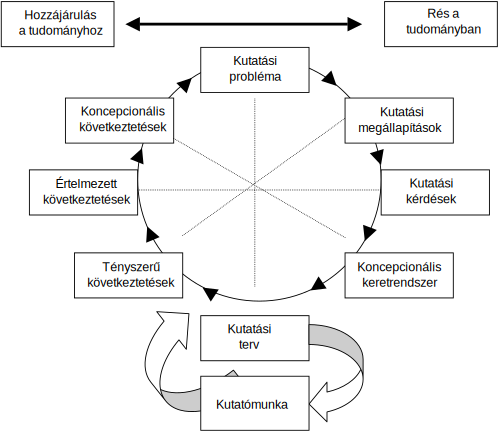
\includegraphics{ábrák/doktori-kutatás-vizualizációja_Leshem.pdf}
\caption{Doktori kutatás módszertanának vázlata (Leshem és Trafford
ábrája nyomán {[}20{]})}\label{fig:doktori}
}
\end{figure}

A javasolt módszertan mentén haladva először a megfogalmazott kutatási
kérdéseket mutatom be, majd a koncepcionális keretrendszert végül az
alkalmazott módszereket és a kutatási szerkezeti felépítését

\hypertarget{kutatuxe1si-kuxe9rduxe9sek}{%
\subsection{Kutatási kérdések}\label{kutatuxe1si-kuxe9rduxe9sek}}

Az alapkérdés megválaszolásának érdekében az alapkérdést felbontandó a
következő kutatási kérdéseket fogalmaztam meg:

\begin{itemize}
\tightlist
\item
  \textbf{KK1:} Vannak-e és melyek a nyílt fejlesztési modellből
  származó termékeknek olyan egyedi sajátosságai amelyek hatással
  lehetnek a biztonságra?
\item
  \textbf{KK2:} A magas biztonsági követelményű rendszerek hogyan
  kerülhetnek kapcsolatba FLOSS elemekkel?
\item
  \textbf{KK3:} Melyek a LIRE védelmének általános irányelvei?
\end{itemize}

Az első kérdés esetében kézenfekvő, hogy ilyen nagy területet átfogó
analízist csak szekunder kutatás segítségével, minél nagyobb számú
kutatási anyag tartalmi elemzésével lehet elvégezni. Ahhoz, hogy az
KK1-re kapott válasz érvényességét meg lehessen becsülni először tehát
meg kell állapítani, hogy a tudományos kutató közösség milyen mélységben
foglalkozott a kérdéskörrel. Ezt követően fel kell mérni, hogy a FLOSS
egyáltalán milyen (nem feltétlenül biztonság specifikus) sajátosságokkal
rendelkezik, mert csak így biztosítható a célkitűzésben megfogalmazott
teljeskörűség, objektivitás és függetlenség. Végül az összes azonosított
sajátosságból ki lehet zárni azokat amelyeknek nincs biztonsági
vonatkozása és rendszerbe lehet foglalni a biztonsági hatást gyakorló
FLOSS sajátosságokat. Ennek az elképzelésnek megfelelően az KK1-et az
alábbi kérdésekre bontottam:

\begin{itemize}
\tightlist
\item
  \textbf{KK4:} A FLOSS hatásai mennyire kutatottak a
  információbiztonság egyes területein?
\item
  \textbf{KK5:} Melyek a nyílt fejlesztési modell egyedi
  jellegzetességei?
\item
  \textbf{KK6:} Mely sajátosságok esetén azonosítható konkrét biztonsági
  hatás?
\end{itemize}

Amennyiben léteznek befolyásoló tényezők (KK1) és a LIRE kapcsolatba
kerülhet FLOSS elemekkel (KK2), érdemes beazonosítani LIRE-re vonatkozó
közvetlen hatásokat. Az ismert és esetleg ismeretlen hatások
beazonosítását követően felmerül a kérdés, hogy ezek a hatások
javíthatják-e a LIRE biztonsági szintjét, illetve védekezhetünk-e
valamilyen módon az általuk okozott kockázatok ellen. Ennek alapján a
következő kérdéseket fogalmaztam meg:

\begin{itemize}
\tightlist
\item
  \textbf{KK7:} A FLOSS sajátosságok milyen hatást gyakorolnak a
  Létfontosságú Információs Rendszerelemekre
\item
  \textbf{KK8:} Melyek azok a hatások amelyek már ismertek, milyen
  megoldásokat alkalmaznak a gyakorlatban?
\item
  \textbf{KK9:} Milyen további hatások létezhetnek?
\item
  \textbf{KK10:} A negatív hatásokat milyen szabályozásbeli, szervezeti
  és technikai óvintézkedések foganatosításával lehet elkerülni, a
  pozitív hatásokat hogyan lehet kihasználni?
\end{itemize}

A precíz válasz érdekében az KK10 szintén további bontást igényelt. Itt
a következő kérdéseket fogalmaztam meg:

\begin{itemize}
\tightlist
\item
  \textbf{KK11:} Milyen intézkedésekkel csökkenthető a FLOSS
  használatának kockázata?
\item
  \textbf{KK12:} Melyek a kutatóközösség által javasolt módszerek?
\item
  \textbf{KK13:} Mely biztonsági problémák kezelésére nincs bevett
  gyakorlat?
\end{itemize}

A kutatási kérdések teljes hierarchiáját és a kutatási kérdésekhez
fűződő kapcsolatát a \ref{fig:KK}. ábra mutatja be.

\begin{figure}
\hypertarget{fig:KK}{%
\centering
\includegraphics[width=1\textwidth,height=\textheight]{ábrák/Research_Questions.pdf}
\caption{Kutatási kérdések hierarchiája (szerkesztette a
szerző)}\label{fig:KK}
}
\end{figure}

A \ref{sec:CELKITUZESEK} fejezetben bemutatott célkitűzéseket
(KC-{[}1-4{]}) Punch kutatási módszertanát követve a fent bemutatott
kérdések alapján fogalmaztam meg. Az értekezés további részében a
célkitűzések jelölésrendszerét használom.

\hypertarget{koncepcionuxe1lis-keretrendszer}{%
\subsection{Koncepcionális
keretrendszer}\label{koncepcionuxe1lis-keretrendszer}}

Az alkalmazott kutatási módszertan következő lépéseként a
\ref{fig:ConFW}. ábrán bemutatott koncepcionális keretrendszert
állítottam össze. Innen kiolvashatóak a kutatás szükséges lépései, a
kutatás során feldolgozott információforrások és a várt eredmények.

\begin{figure}
\hypertarget{fig:ConFW}{%
\centering
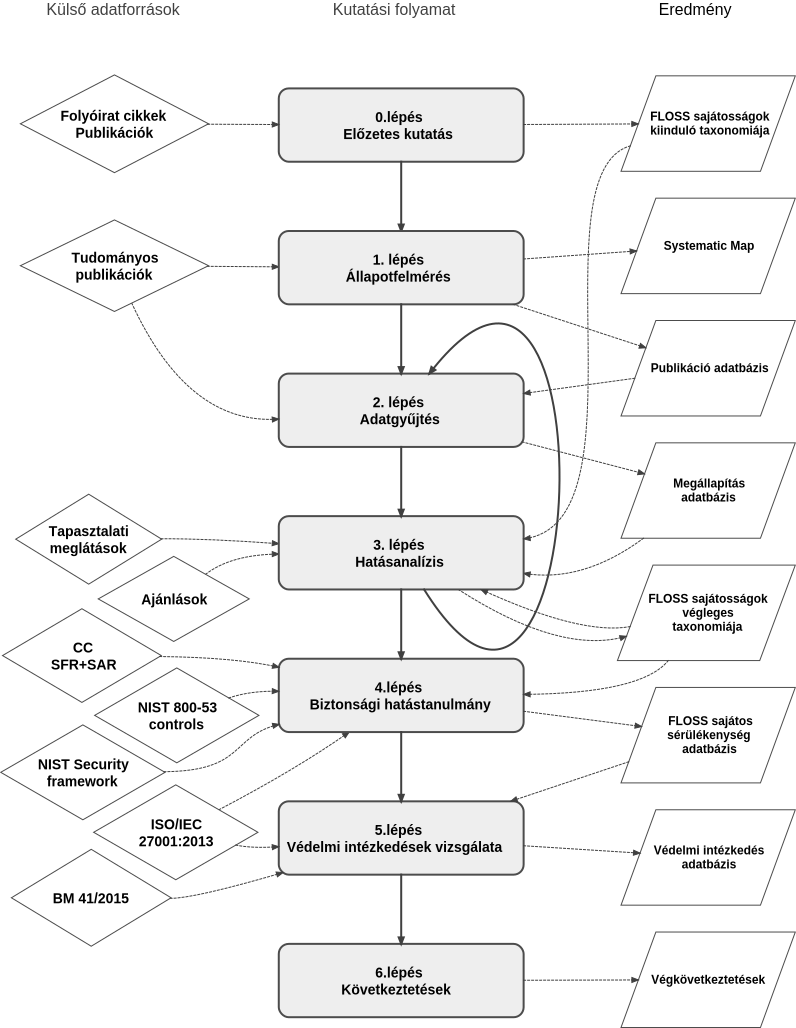
\includegraphics{ábrák/Conceptual_Framework.pdf}
\caption{A kutatás koncepcionális keretrendszere (szerkesztette a
szerző)}\label{fig:ConFW}
}
\end{figure}

Az ábra első oszlopában találhatóak a felhasznált információforrások. A
kutatás elsődleges információforrása a feldolgozott cikkekből és
tanulmányokból manuálisan kigyűjtött adatok, de a hatásanalízis során
meglévő ajánlásokat, illetve létező, aktívan használt keretrendszerek
(ISO/IEC 27001, NIST 800-53, Common Criteria) javaslatait is figyelembe
vettem. Ezáltal biztosított a kutatási célokban megfogalmazott (KC-2)
teljeskörűség mind a sajátosságok, mind a biztonsági hatások
tekintetében.

A második oszlopban lekerekített téglalpokkal jelölt kutatási folyamat
lépéseiből látható, hogy a kutatás adatgyűjtő-elemző része ciklikus
jellegű, azaz a hatásanalízis során finomított taxonomia és a biztonsági
hatások bővülő kategóriái az adatgyűjtés során újra felhasználásra
kerültek. A ciklikus megvalósításra részben azért volt szükség, mert a
címkézés során létrehozott új kategóriákat a már feldolgozott
publikációk anyaga esetében is értelmezni kellett, másrészt az
analízis-szintézis szakasz elég hosszú időt vett igénybe, és az
időközben megjelent új publikációkat folyamatosan rendszerbe kellett
illeszteni.

A harmadik oszlopban feltüntetett eredmények olyan dokumentumokat és
adatbázisokat jelölnek, amelyek a kutatás további fázisaiban, más
kutatásokban vagy a gyakorlatban felhasználható információt és adatokat
tartalmaznak.

\hypertarget{alkalmazott-kutatuxe1si-muxf3dszerek}{%
\subsection{Alkalmazott kutatási
módszerek}\label{alkalmazott-kutatuxe1si-muxf3dszerek}}

Az KC-1.1 elérésre Petersen által javasolt szisztematikus
feltérképezés\footnote{Systematic Mapping Study} módszerét alkalmaztam
{[}21, 22{]}.

A szisztematikus térképezés módszere széles körben alkalmazott praktikus
eszköz a szoftvermérnöki területek osztályozási feladataira és a kutatás
struktúrájának felmérésére. Ez az analízis a publikációk kategóriánkénti
sűrűségére koncentrál, így meghatározható a terület kategóriánkénti
becsült fedettsége. A klasszikus szisztematikus térképezés nem merül el
a részletekben, a publikációkat nem elemzi részletesen. A javasolt
módszerhez képest esetemben mélyebb elemzésre volt szükség -- közeledve
a klasszikus szisztematikus forráselemzéshez {[}23{]} -- ugyanis a
publikációk alkalmazott módszertanát és eredményeinek típusát is meg
akartam határozni.

A FLOSS sajátosságok kategóriáihoz az előzetes kutatások során {[}24{]}
előállított FLOSS sajátosság taxonomia vázlatot használtam fel amelyet a
az összegyűjtött anyagok segítségével fokozatosan pontosítottam.

A szisztematikus feltérképezés alapját képező gyűjtőmunka kettős célt
szolgált. Egyrészt a szisztematikus feltérképzés segítségével
meghatározhatóvá vált, hogy mely területek milyen mértékben kutatottak,
azaz az eredmények várható megbízhatósága és teljessége milyen szintű
lesz az egyes területeken, másrészt az összegyűjtött és felcímkézett
forrásanyag alapját képezhette a kutatás következő analitikus fázisának.

A feltérképezést és adatgyűjtést 2016-ban végeztem el, viszont a teljes
anyagmennyiség feldolgozása és analízise sok időt vett igénybe, ezért
eredeti publikáció adatbázist folyamatosan frissítésekkel láttam el. Az
SMS adatok azonban a korábbi állapotot tükrözték, így a kategorizálást
azonos keresési metodika használata mellett megismételtem. A frissítését
2020-ban végeztem, így az irodalomkutatás a 2020 elején fennálló
állapotot tükrözi.

Az KC-1.2, KC-1.3 és KC-2 célok elérése érdekében az analízis-szintézis
módszertanát alkalmaztam. Az első fázisban összegyűjtött és folyamatosan
kiegészített dokumentumokból felépítettem a FLOSS sajátosságainak lehető
legteljesebb modelljét, majd a modell alapján meghatároztam a biztonsági
hatásokkal kapcsolatos jellemzőket illetve -- amennyiben voltak ilyenek
-- a javasolt megoldásokat. Az KC-1 analízis kimenetének szintézisével
határoztam meg a KC-2 alatt megfogalmazott területeket és hatáspontokat,
illetve becslést adok a be nem azonosított sajátosságok és védelmi
intézkedések számát illetően.

A FLOSS sajátosságok és a hatáspontok modelljét, valamint a magas
biztonsági rendszerekre vonatkozó ajánlásokat és előírásokat összevetve
szintézis segítségével határoztam meg a KC-3 alatt megfogalmazott
lehetséges védelmi intézkedéseket. A védelmi intézkedések kialakítását a
NIST 800-53 security overlay mechanizmusa inspirálta. A NIST security
overlay egységes sablon kialakítását javasolja a speciális
követelményeket támasztó ágazatokhoz és szervezetek számára {[}25{]}.
Hasonló elképzelés mentén terveztem a nyílt forrást alkalmazó és magas
biztonsági követelményeknek megfelelni kívánó szervezetek --
különösképpen a Létfontosságú Rendszerelemek -- számára olyan intézkedés
overlay-t képezni, amely a meglévő szabályozást kiegészítve felhívja a
figyelmet a FLOSS esetében eltérően vagy különös figyelemmel kezelendő
pontokra.

A NIST 800-53 overlay elképzelésével ellentétben helyhiány miatt csak a
különbözetet adom meg, amelyekkel az eredeti szabályokat szükség esetén
ki lehet egészíteni, értelemszerűen az általános esetben érvényes
eljárásokat továbbra minden esetben alkalmazni kell.

Végezetül, a sajátosságokból eredő hatásokat és a megállapított védelmi
intézkedéseket összevetettem a vonatkozó ajánlásokkal és hazai
szabályozással az esetleges fehér foltok feltárása érdekében.

\hypertarget{az-uxe9rtekezuxe9s-feluxe9puxedtuxe9se-jeluxf6luxe9srendszere}{%
\subsection{Az értekezés felépítése,
jelölésrendszere}\label{az-uxe9rtekezuxe9s-feluxe9puxedtuxe9se-jeluxf6luxe9srendszere}}

A második fejezet a kutatás tárgyával és irodalmával foglalkozik. Itt
definiálom a kutatás témájának kereteit és a vizsgált területeket.
Ugyanitt találhatóak az irodalomkutatás összefoglaló eredményei amelyek
a kutatási célkitűzésekkel összhangban az egyes biztonsági területek
vizsgálatának alaposságát kívánják meghatározni, amely alapján az
eredmények teljeskörűsége végül becsülhető. A második fejezet végén a
Létfontosságú Rendszerelemek és a nyílt forrás kapcsolódási pontjait
vizsgálom, amely alapul szolgál a következő fejezetekben tárgyalt
biztonsági analízishez.

A nyílt forrás belső és külső egyedi jellegzetességeivel az fejezetek
közötti egyensúly megtartása érdekében két külön fejezet foglalkozik. A
harmadik fejezet a FLOSS belső, azaz külső tényezőktől független
tulajdonságait vizsgálja, míg a negyedik fejezet a külső tényezők és a
FLOSS kapcsolatrendszeréből adódó sajátosságokat elemzi. A fejezetek
KK1-ben megfogalmazott kérdésre adnak választ, és az itt azonosított
egyedi sajátosságok alapján válik végül lehetségessé a KK3 kérdésének
megválaszolása.

A harmadik és negyedik fejezetben alkalmazott rendszertant a
\ref{fig:FLOSSSaj}. ábra mutatja be. Az egyes fejezeteket a könnyű
azonosíthatóság érdekében az itt meghatározott kóddal jelöltem
FS-főkategória-alkategória alakban. E jelölésrendszernek megfelelően a
nyílt forrás ``Szabályozás'' kategóriájába eső ``Összetett licencelés''
az FS-SZ-L, míg a ``Fejlesztési folyamatok'' kategória ``Tervezéssel''
kapcsolatos elemzése az FS-F-P kódot kapta (lásd: \ref{fig:FLOSSSaj}.
ábra).

\begin{figure}
\hypertarget{fig:FLOSSSaj}{%
\centering
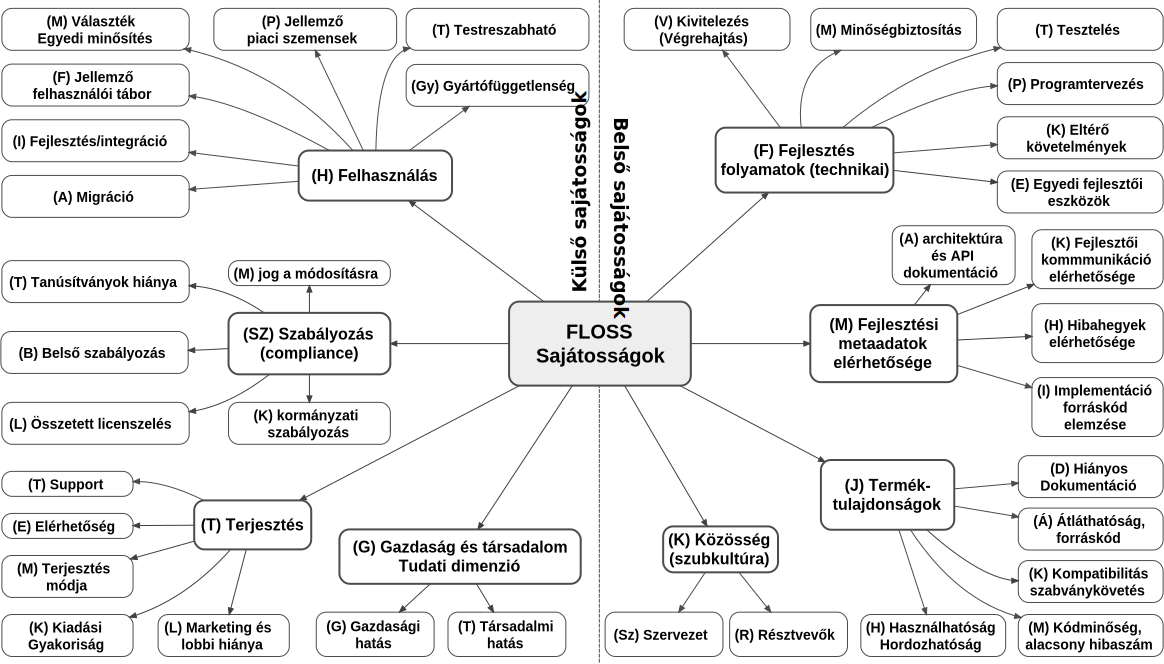
\includegraphics{ábrák/FLOSS-jellegzetességek.pdf}
\caption{A nyílt forrás sajátosságainak rendszertana (szerkesztette a
szerző)}\label{fig:FLOSSSaj}
}
\end{figure}

A sajátosság kategóriák mindegyikénél meghatároztam a felmerülő
sérülékenységeket valamint az azonosított javaslatokat. A
sérülékenységeket `S' míg a javaslatokat `J' kezdetű kód jelöli, amelyet
a kategória betűkódja, majd az egyediséget biztosító kétjegyű szám
követ. Ennek megfelelően a Fejlesztés (F) kategóriában azonosított első
lehetséges sérülékenységet az SF01, míg az első javaslatot JF01 kód
jelöli.

A további fejezetek az azonosított FLOSS sajátosságok hatását elemzik a
Létfontosságú Rendszerelemek területén. Ez két lépésben történik. A
negyedik fejezetben a NIST Cyber Security Framework által definiált
információbiztonsági irányelvek alapján vizsgálom a nyílt forrás
sajátosságainak lehetséges hatásait az egyes lépésekre, végül az ötödik
fejezetben az azonosított feladatokat összevetem a Létfontosságú
Rendszerelemek információbiztonsági követelményeit definiáló hazai
szabályozással.

Az egyértelmű azonosíthatóság érdekében a biztonsági irányelvek esetében
megtartottam az eredeti (angol nyelvű) dokumentum kódjait, a megfelelő
fejezeteket ez a kód jelöli. Ennek megfelelően például a ``Védelem''
(Protection) alá tartozó ``Adatbiztonság'' (Data Security) elvével
foglalkozó részt PR.DS kód jelöli az eredeti jelöléssel összhangban.

A bizonsági irányelvek és FLOSS sajátosságok összevetése során
azonosított lehetséges védelmi intézkedéseket `V' kód jelöli, amelyet a
biztonsági irányelv kategória kódja, majd folyamatos számozás követ. Így
tehát a Helyreállítás (Recovery) kategória alatt azonosított védelmi
intézkedések VRC{[}N{]} alakú kódot kapnak, ahol N az 1-től induló
folyamatos számozást jelenti.

\hypertarget{kutatuxe1s-tuxe1rgya-uxe9s-irodalma}{%
\chapter{Kutatás tárgya és
irodalma}\label{kutatuxe1s-tuxe1rgya-uxe9s-irodalma}}

\hypertarget{luxe9tfontossuxe1guxfa-rendszerelemek-uxe9s-informuxe1ciuxf3s-rendszerelemek}{%
\section{Létfontosságú Rendszerelemek és Információs
Rendszerelemek}\label{luxe9tfontossuxe1guxfa-rendszerelemek-uxe9s-informuxe1ciuxf3s-rendszerelemek}}

A Létfontosságú Rendszerelemek, régebbi nevén Kritikus Infrastruktúrák
védelme korunk egyik legfontosabb biztonsági kihívása. Értekezésemben a
létfontosságú rendszerelemek működési hátterét biztosító Létfontosságú
Információs Rendszerelemekre gyakorolt hatásokkal foglalkozom.

\hypertarget{luxe9tfontossuxe1guxfa-rendszerelemek-kritikus-infrastruktuxfaruxe1k}{%
\subsection{Létfontosságú Rendszerelemek (Kritikus
Infrastruktúrák)}\label{luxe9tfontossuxe1guxfa-rendszerelemek-kritikus-infrastruktuxfaruxe1k}}

A társadalom működésének megzavarását célzó támadások stratégiai
célpontjai a kritikus infrastruktúrák. A kritikus infrastruktúrák
működtetéséhez szükséges infokommunikációs rendszerek rendkívül csábító
támadási felületet jelentenek, hiszen a támadó fél alacsony erőforrás és
eszközigénnyel is jelentős károkat tud okozni, ráadásul a globális
jellegből adódóan mindezt biztonságos távolságból teheti meg. A kritikus
információs infrastruktúrák közötti szoros kapcsolat jelentősen
megnöveli az információs társadalom sebezhetőségét. Az új típusú
fenyegetések annál hangsúlyosabban vannak jelen, minél magasabb szintű e
rendszerek integráltsága, komplexitása és egymástól való függősége.
Ennek megfelelően egyre erősebb az igény a megfelelő szintű biztonság
elérésére. {[}16{]}

A fenyegetés súlyát növeli, hogy a kritikus infrastruktúrák elleni
információs támadások célja feltehetően nem gazdasági előnyszerzés hanem
politikai vagy katonai célok elérése, a támadó pedig nem egyedül álló
személy vagy kisebb csoport, hanem jelentős erőforrásokkal rendelkező
nemzetállam.

Könnyen felismerhető, hogy ez a fajta katonai felfogás jól alkalmazható
az egymással szoros függőségi kapcsolatban álló kritikus infrastruktúrák
esetén, így e rendszerek súlyponti elemeinek megfelelő védelme fontos
nemzetbiztonsági kérdés.

A létfontosságú rendszerek és létesítmények azonosításáról,
kijelöléséről és védelméről a 2012. évi CLXVI. törvény rendelkezik.

Létfontosságú rendszerelemnek minősül a törvény mellékletében
meghatározott ágazatok valamelyikébe tartozó eszköz, létesítmény vagy
rendszer olyan rendszereleme, amely ``elengedhetetlen a létfontosságú
társadalmi feladatok ellátásához - így különösen az egészségügyhöz, a
lakosság személy- és vagyonbiztonságához, a gazdasági és szociális
közszolgáltatások biztosításához -, és amelynek kiesése e feladatok
folyamatos ellátásának hiánya miatt jelentős következményekkel járna.''
{[}26{]}

A törvény szerint európai létfontosságú rendszerelemnek minősül a
törvény alapján kijelölt ``olyan létfontosságú rendszerelem, amelynek
kiesése jelentős hatással lenne - az ágazatokon átnyúló kölcsönös
függőségből következő hatásokat is ideértve - legalább két
EGT-államra''.

Nemzeti létfontosságú rendszerelemnek minősül a törvény alapján kijelölt
``olyan létfontosságú rendszerelem, amelynek kiesése a létfontosságú
társadalmi feladatok folyamatos ellátásának hiánya miatt jelentős hatása
lenne Magyarországon''.

Létfontosságú rendszerelem védelmének ``a létfontosságú rendszerelem
funkciójának, folyamatos működésének és sértetlenségének biztosítását
célzó, a fenyegetettség, a kockázat, a sebezhetőség enyhítésére vagy
semlegesítésére irányuló'' valamennyi tevékenységet nevezzük.

A kritikus infrastruktúrák védelmi szempontból legfontosabb jellemzői:

\begin{itemize}
\tightlist
\item
  kölcsönös függőség,
\item
  hálózatszerűség,
\item
  domino-elv hatás,
\item
  működési sajátosság,
\item
  kiterjedés-elhelyezkedés,
\item
  informatikai háttér.
\end{itemize}

Az infrastruktúrák közötti fennálló függőség miatt jelentős negatív
hatást lehet gyakorolni:

\begin{itemize}
\tightlist
\item
  az információs társadalom szervezett működési rendjére, minőségére,
  dinamikus egyensúlyára;
\item
  vezetési rendszerének hatékonyságára, integritására;
\item
  a vezetés struktúrájára, szervezettségi fokára;
\item
  a belső és külső kommunikációra, a kapcsolati viszonyokra és
\item
  az adott szervezet operatív vezethetőségére. {[}27{]}
\end{itemize}

A dominó elv értelmében tényleges valószínűsége van annak, hogy a
kölcsönös függőség miatt egyetlen esemény láncreakciót indítson be,
amelynek végül több infrastruktúra működését és rendelkezésre állását
befolyásolja.

A kritikus infrastruktúra védelem három fő pilléren - megelőzés,
felkészülés és ellenálló képesség -- támaszkodva törekszik az
infrastruktúrák biztonságos működését elősegítő intézkedések
megtételére. A megelőzés első sorban a különböző leállások,
meghibásodások kockázatának lehető legkisebb szintre történő
csökkentésére irányul. A megelőzési tevékenységek közé soroljuk a
veszélyeztető tényezők elemzését, a kockázatok feltérképezését és a
legérzékenyebb pontok beazonosítását, amelyek alapján a szükséges
védelmi szint meghatározható. A felkészülés feladata a tulajdonosok,
üzemeltetők, felügyeleti szervek és központi államigazgatási szervek
felkészítése, melynek célja, hogy az érintettek között aktív és hatékony
kommunikáció, valamint eredményes és célravezető együttműködés alakuljon
ki. Az ellenálló képesség megerősítéséhez három összetevő biztosítása
szükséges:

\begin{itemize}
\tightlist
\item
  alternatívák kialakítása, a kieső rendszer mielőbbi pótlásának
  érdekében;
\item
  visszaállító képesség, hogy az esemény után a lehető leghamarabb
  visszaálljon az eredeti állapot;
\item
  végül a sebezhető pontok csökkentése, melynek segítségével az
  infrastruktúra ellenálló képessége megnövekszik tekintve, hogy a
  kritikusság mértékét immár kevesebb kockázati faktor határozza meg.
  {[}28{]}
\end{itemize}

\hypertarget{luxe9tfontossuxe1guxfa-rendszerelemek-fejlux151duxe9se}{%
\subsubsection{Létfontosságú rendszerelemek
fejlődése}\label{luxe9tfontossuxe1guxfa-rendszerelemek-fejlux151duxe9se}}

A napjainkban is zajló cselekvési hullámot a 2001-ben elkövetett
terrortámadások indították meg. A háttérbe szoruló hagyományos
hadviselés helyét az új, nehezen azonosítható fenyegetések vették át,
amelyek egyre inkább irányulnak kifejezetten a lakosság elrettentésére
és károkozásra, mint a fegyveres erők ellen.

A NATO Felsőszintű Polgári Veszélyhelyzet Tervezési Bizottsága 2001-ben
kezdte meg a kritikus infrastruktúra védelemmel kapcsolatos irányelvek
kidolgozását, amelynek keretében a 2003-ban elfogadott irányelvben a
megalkotta saját, tevékenységéhez illeszkedő kritikus infrastruktúra
fogalmát, amely ``azokat a létesítményeket, szolgáltatásokat és
információs rendszereket jelenti, amelyek olyan létfontosságúak a
nemzetek számára, hogy működésképtelenné válásuknak vagy
megsemmisülésüknek gyengítő hatása lenne a nemzet biztonságára, a
nemzetgazdaságra, a közegészségre, a közbiztonságra és a kormány
hatékony működésére''\footnote{A NATO Polgári Védelmi Bizottsága által
  megfogalmazott kritikus infrastruktúra védelmi koncepció alapján
  (Critical Infrastructure Protection Concept Paper
  EAPC(SCEPC)D(2003)15).}{[}28{]}.

Az események az Európai Uniót is cselekvésre késztették, felvetve az
egységes, stratégia alapú, közösségi infrastruktúrák védelmére irányuló
jogi szabályozás igényét. Az Európai Unión belül 2004-től kezdve több, a
Létfontosságú Rendszerelemekkel kapcsolatos dokumentum jelent meg:

\begin{itemize}
\tightlist
\item
  Communication from the Commission to the Council and the European
  Parliament: Preparedness and consequence management in the fight
  against terrorism, COM (2004) 701 final, Bruxelles, 20 October 2004;
\item
  Communication from the Commission to the Council and the European
  Parliament: Critical Infrastructure Protection in the fight against
  terrorism, COM (2004) 702 final, Bruxelles, 20 October 2004;
\item
  Green paper on a European programme for critical infrastructure
  protection (presented by the Commission) COM (2005) 576 final,
  Bruxelles, 17 November 2005.
\end{itemize}

Ezeket követte a 2008/114/EC direktíva megjelenése\footnote{Council
  Directive 2008/114/EC of 8 December 2008 on the identification and
  designation of European critical infrastructures and the assessment of
  the need to improve their protection.}, amely értelmében a legfőbb és
végső felelősség a tagállamokat és az infrastruktúra üzemeltetőjét
terheli {[}29{]}.

Az Európai Unió kritikus infrastruktúra fogalma részletesebb,
kifejezetten az Unió egységére irányul, de mégis általánosságban
fogalmaz. A Zöld Könyv definíciója szerint azok a fizikai eszközök,
szolgáltatások, információs technológiai létesítmények, hálózatok és
vagyontárgyak tekinthetők kritikus infrastruktúrának, melyek
megrongálása vagy elpusztítása súlyos hatással lenne az európaiak
egészségére, békéjére, biztonságára, vagy gazdasági jólétére illetve az
EU és a tagállamok kormányainak hatékony működésére {[}30{]}.

A Zöld Könyv elsődleges célja, hogy felhívja a figyelmet egy-egy terület
meghatározó és megválaszolatlan kérdéseire, illetve aktív
együttműködésre ösztönözze az egyes szektorok képviselőit, mint a
létfontosságú infrastruktúrák védelmének kulcsszereplőit. Központi eleme
a szubszidiaritás\footnote{A döntéseket azon a lehető legalacsonyabb
  szinten kell meghozni, ahol az optimális informáltság, a döntési
  felelősség és a döntések hatásainak következményei a legjobban
  átláthatók és érvényesíthetők.} került, amely szerint a létfontosságú
rendszerelemek védelme elsősorban nemzeti hatáskör, vagyis a felelősség
első sorban a tagállamokat, tulajdonosokat és üzemeltetőket terheli.

A későbbi irányelv kidolgozásához a Zöld Könyv három védelmi stratégiát
kínált, amelyekre a védelmi tevékenység felépíthető. Egy összetett
megközelítés, amely a szándékos, ártó jelleg támadásokkal és a
természeti katasztrófák veszélyeivel egyaránt számol, de a terrorizmust
nem kezeli kiemelt kihívásként. Egy komplex és rugalmas megközelítést,
amely tekintettel van az egyéb támadásokból származó fenyegetésekre és a
természeti katasztrófák okozta veszélyekre, de középpontjában az ártó
szándékú cselekmények vagyis a terrorizmus áll. Végül pedig egy
kifejezetten a terrorizmusra összpontosító megközelítést, amely nem
tekint prioritásnak más egyéb veszélyeztető tényezőt. {[}31{]}

Meghatározásra került a közösség érdekei szerint elsődleges és magasabb
szintű létfontosságú rendszerelemek, azaz európai létfontosságú
rendszerelemek\footnote{European Critical Infrastructure, ECI} fogalma.
A másodlagos, de a tagállamok szempontjából kiemelt jelentőséggel bíró
csoport a nemzeti létfontosságú rendszerelemek\footnote{National
  Critical Infrastructure, NCI} nevet kapta, amelyek létesítésük szerint
egy adott tagállam területén találhatóak, de sérülésük, leállásuk,
megsemmisülésük esetén hatásuk csak az ország határain belül érezhető
{[}28{]}. Fentieken túl a Zöld Könyv felhívta a figyelmet az Unió
területén kívül található olyan infrastruktúrákra, amelyek esetleges
üzemzavara, vagy megsemmisülése hatással lehet az Európai Unió
tagállamaira, azok infrastruktúráira, működésére.

Az európai kritikus infrastruktúrák azonosításáról és kijelöléséről,
valamint védelmük javítása szükségességének értékeléséről szóló
2008/114/EK Irányelvet 2008. december 8-án fogadták el. Az Irányelv a
Zöld Könyvvel, az európai programmal és az ágazati specifikumokkal
összhangban, határozta meg a létfontosságú rendszerelemek azonosítására
és kijelölésére vonatkozó eljárások, eszközök és elvek halmazát. Az
Irányelv első és legfontosabb tétele, hogy a kihirdetéstől számított két
éven belül a megvalósításhoz szükséges intézkedéseket a tagállamoknak
végre kellett hajtaniuk. A 2011-ben megjelent EU belbiztonsági Stratégia
tovább erősítette a kritikus infrastruktúrák védelmének szükségességét
és napirenden tartását, különös tekintettel a modern technológiák által
biztosított lehetőségeket is kiaknázó szervezett bűnözésre {[}31{]}.

A hálózati és információs rendszerek és szolgáltatások biztonságával
foglalkozó (EU) 2016/1148 iránnyelv (NIS irányelv) 2016 július 6.-án
lépett érvénybe. Az irányelv előírja, hogy a határokon átnyúló
együttműködés és kommunikáció elősegítése érdekében valamennyi
tagállamon belül létre kell hozni egy nemzeti kapcsolattartó pontot,
amely a hálózati és információs rendszerek biztonságával kapcsolatos
kérdések koordinálásáért felel. Az irányelv értelmében a biztonsági
eseményekről bejelentést kell kapniuk a hatóságoknak vagy
számítógép-biztonsági eseményekre reagáló csoportoknak (röviden
CSIRT-eknek), amelyek szükség esetén a központon keresztül megoszthatják
a biztonsági eseményekkel kapcsolatos információkat. A CSIRT-ek hálózata
gyors és hatékony operatív működést tesz lehetővé. A tagállamoknak
biztosítaniuk kell, hogy olyan jól működő CSIRT-ekkel -- más néven
hálózatbiztonsági vészhelyzeteket elhárítós csoportokkal (CERT)
rendelkezzenek, amelyek hatékonyan képesek biztonsági események és
kockázatok kezelésére és az európai szintű együttműködésre {[}32{]}.

\hypertarget{magyarorszuxe1gi-tevuxe9kenysuxe9gek}{%
\subsubsection{Magyarországi
tevékenységek}\label{magyarorszuxe1gi-tevuxe9kenysuxe9gek}}

NATO tagságunk révén betekintést nyertünk a kritikus infrastruktúra
védelmi kezdeményezésekbe, 2001-2002-ben országos adatgyűjtés keretében
felmérték az infrastruktúrák helyzetét, amely alapján megállapításra
került, hogy kormányzati szint döntésekre van szükség ahhoz, hogy az
infrastruktúrák védelmével kapcsolatos tevékenység megfelelő háttere
biztosítva legyen. {[}31{]}

A létfontosságú rendszerelemek nemzetközi védelmi programjának
kidolgozásában Magyarország már teljes jogú tagállamként vett részt. A
2006 decemberében elfogadott irányelv-tervezet alapján megkezdődhetett
az érdemi munka hazánkban is, 2007-ben a tárcák és országos hatáskörű
szervek együttműködésével vette kezdetét a magyar nemzeti védelmi
program kidolgozása. Megszületett a magyar Zöld könyv, mely már
érvényesítette a kritikus infrastruktúrák ágazati szintű besorolását. A
Zöld könyv megállapítása szerint: ``az infrastruktúrák folyamatos
működése, kockázati tényezőkkel szembeni ellenálló képességének növelése
a lakosság, az infrastruktúra tulajdonosok, üzemeltetők, valamint a
gazdaság szereplői és az állam számára egyaránt kiemelt fontossággal
bír, a biztonságos működést elősegítő környezet és intézkedések ezért
értéket képviselnek.''

A 2080/2008. (VI. 30.) kormányhatározat a Kritikus Infrastruktúra
Védelem Nemzeti Programjáról kihirdette a további konzultációk és
folyamatok alapjául szolgáló zöld könyvet. Elrendelte az ágazati
konzultációk lefolytatását, amelyhez ágazatonként minisztériumot, vagy
országos hatáskörű szervet rendelt felelősként; valamint szabályozási
koncepció kidolgozását írta elő {[}28{]}. A határozat jogszabályi
formába ültette át a Zöld könyvet, így megindulhatott a párbeszéd a
potenciális üzemeltetők, kritikus infrastruktúra tulajdonosok és az
érintett hatóságok között. A következő lépés a 1249/2010. (XI.19.) Korm.
határozat kiadása volt, mely lényegében az irányadó EU irányelv
implementációja érdekében végrehajtandó kormányzati feladatok
katalógusát adta meg, amit hamarosan követet az új katasztrófavédelmi
norma, a katasztrófavédelemről és a hozzá kapcsolódó egyes törvények
módosításáról szóló 2011. évi CXXVIII. törvény és végrehajtási
rendelete, a 234/2011 (XI. 10.) Korm. rendelet kiadása. A jogszabály a
BM Országos Katasztrófavédelmi Főigazgatóság (a továbbiakban: OKF)
szervezetén belül létrehozta az iparbiztonsági főfelügyelőséget, amely a
súlyos balesetek elleni védekezésért, a veszélyesáru-szállítás
felügyeletéért és a kritikus infrastruktúrák védelméért felelős {[}1{]}.

A létfontosságú rendszerek és létesítmények azonosításáról,
kijelöléséről és védelméről szóló 2012. évi CLXVI. törvényt (Lrtv.) az
Országgyűlés 2012. november 12-én fogadta el. A törvény célja a
létfontosságú rendszerelemek azonosítása, illetve a kijelölést követően
a megfelelő szint védelem biztosítása. Az Lrtv. az értelmező
rendelkezésekben található alapvető fogalmak meghatározásán túl,
körvonalazza a nemzeti és az európai kritikus infrastruktúrák
kijelölésének rendjét, rendelkezik az üzemeltetői biztonsági terv
készítésének kötelezettségéről, a biztonsági összekötő személy
kijelöléséről, a nyilvántartás és ellenőrzés szabályairól, valamint a
szankcionálásról. Külön rendelkezéseket tartalmaz az energia ágazat
vonatkozásában, amelyeket az ágazati kormányrendelettel együtt kell
értelmezni.

A keretszabályozás markáns eleme lett a Lrtv. végrehajtási rendeletének
tekinthető 65/2013. (III. 8.) kormányrendelet, amely részletesen
szabályozza az azonosítási és kijelölési eljárás általános folyamatát,
beleértve az azonosítási jelentést, az ágazati kijelölő és javaslattevő
hatóság szerepét, és a szakhatósági állásfoglalást. Külön rendelkezik az
európai létfontosságú rendszerelemek kijelölési eljárásáról, a
biztonsági összekötő személy általános követelményeiről, amelyeket az
ágazati kormányrendeletek további, szakmai feltételekkel egészítenek ki.
A rendelet -- a honvédelmi létfontosságú rendszerelemek kivételével --
OKF-et, jelöli ki az európai és nemzeti létfontosságú rendszerelemek
nyilvántartó hatóságaként. {[}31{]}

2013-ban megalakult a Létfontosságú Rendszerek és Létesítmények
Informatikai Biztonsági Eseménykezelő Közppontja (LRL IBEK) elnevezésű
szervezet a BM Országos Katasztrófavédelmi Főigazgatóság szervezeti
keretein belül. Feladata -- az állam és az önkormányzatok által
üzemeltetett létfontosságú rendszerek és létesítmények kivételével -- a
nemzeti létfontosságú rendszerek és létesítmények védelmével kapcsolatos
hálózatbiztonsági tevékenység ellátása {[}33{]}.

A 2016/1148/EU (NIS) irányelvnek való megfelelés érdekében megszületett
a 185/2015. (VII. 13.) Korm. rendelet amely rögzíti a kormányzati
eseménykezelő központ és az eseménykezelő központok (hazai CSIRT)
feladat- és hatáskörét, valamint a biztonsági események kezelésének, a
biztonsági események műszaki vizsgálatának és a sérülékenységvizsgálat
lefolytatásának szabályait.

Mindenképpen említést érdemel még a Magyarország hálózati és információs
rendszerek biztonságára vonatkozó Stratégiájáról rendelkező 1838/2018.
(XII. 28.) Korm. határozat valamint a stratégiát meghatározó kapcsolódó
dokumentum, amely NIS irányelv hazai implementációjához hozzájárulva
foglalkozik a digitális bizalom erősítésének, a digitális infrastruktúra
védelmének és a gazdasági szereplők támogatásának kérdéseivel. A
dokumentum célként jelöli meg -- többek között -- egy könnyen elérhető,
érthető és használható információs bázis kialakítását, a létfontosságú
információs infrastruktúrák maximális védelmének biztosítását, NIS
irányelvben meghatározott együttműködés megindítását valamint a képzés
és kutatás támogatását {[}34{]}.

Az első hálózatbiztonsági eseménykezelő központok Magyarországon az
1990-es évek végén jöttek létre (Hungary-CERT, MIIF CSIRT). A kritikus
információs infrastruktúrák védelmére specializálódott CERT-Hungary
Központ 2005-ben alakult meg, amely aztán 2009-ben Nemzeti
Hálózatbiztonsági Központtá (CERT-Hungary) alakult. Ezekre alapozva
került kialakításra a Nemzeti Kibervédelmi Intézet részeként a
Kormányzati Eseménykezelő Központ (GovCERT-Hungary) 2013-ban, majd
jöttek létre az ágazati eseménykezelő központok {[}33{]}.

\hypertarget{sec:LIRE}{%
\subsection{Létfontosságú Információs Rendszerelemek}\label{sec:LIRE}}

A 2013. évi L. törvény megfogalmazása szerint ``létfontosságú
információs rendszerelem az európai vagy nemzeti létfontosságú
rendszerelemmé a létfontosságú rendszerek és létesítmények
azonosításáról, kijelöléséről és védelméről szóló törvény alapján
kijelölt létfontosságú rendszerelemek azon elektronikus információs
létesítményei, eszközei vagy szolgáltatásai, amelyek működésképtelenné
válása vagy megsemmisülése az európai vagy nemzeti létfontosságú
rendszerelemmé kijelölt rendszerelemeket vagy azok részeit
elérhetetlenné tenné, vagy működőképességüket jelentősen csökkentené''.

A törvény végrehajtási rendeletének definíciója szerint a létfontosságú
információs rendszerek és létesítmények ``a társadalom olyan
hálózatszerű, fizikai vagy virtuális rendszerei, eszközei és módszerei,
amelyek az információ folyamatos biztosítása és az informatikai
feltételek üzemfolytonosságának szükségességéből adódóan önmagukban
létfontosságú rendszerelemek, vagy más azonosított létfontosságú
rendszerelemek működéséhez nélkülözhetetlenek.''

A jogszabályi megfogalmazás egyértelművé teszi, hogy egy kritikus
információs infrastruktúra lehet önmagában is kritikus, illetve
teljesíti a kritikusság kritériumát a többi kritikus infrastruktúra
számára nyújtott nélkülözhetetlen infokommunikációs szolgáltatás által
is. A fenti definíció és a törvény ágazati besorolása alapján a kritikus
információs infrastruktúrák alatt az alábbiakat értjük:

\begin{itemize}
\tightlist
\item
  az energia-ellátó rendszerek rendszerirányító infokommunikációs
  hálózatait;
\item
  a közlekedésszervezés és -irányítás infokommunikációs hálózatait;
\item
  az agrárgazdaságot szabályzó, irányító infokommunikációs hálózatokat;
\item
  az egészségügyi rendszer infokommunikációs hálózatait;
\item
  a pénzügyi szektor infokommunikációs hálózatait;
\item
  az ipari termelést irányító infokommunikációs hálózatokat;
\item
  az infokommunikációs technológiákat;
\item
  a vízellátást szabályzó infokommunikációs hálózatokat;
\item
  a jogrend és a kormányzat infokommunikációs hálózatait;
\item
  a közbiztonság és védelmi szféra infokommunikációs hálózatait.
  {[}16{]}
\end{itemize}

A létfontosságú információs rendszerelemek a létfontosságú
rendszerelemek sajátos veszélyei mellett további hét, jellemzően
aszimmetrikus fenyegetésnek vannak kitéve:

\begin{itemize}
\tightlist
\item
  kiberbűnözés;
\item
  kiberterrorizmus;
\item
  hacktivista mozgalmak;
\item
  programozási/paraméterezési és üzemeltetési hibák.
\end{itemize}

Ezek jelentős károkat eredményezhetnek, negatívan befolyásolhatják az
üzem- és termelés folytonosságot, a hatékony vállalati működést, és az
infrastruktúrák összekapcsolódásából eredő hatások folytán ágazati
szintű problémákat okozhatnak. {[}1{]}

\hypertarget{lre-lire-uxe9s-floss-kapcsolata}{%
\subsection{LRE, LIRE és FLOSS
kapcsolata}\label{lre-lire-uxe9s-floss-kapcsolata}}

Mint láthattuk, a Létfontosságú Információs Rendszerelemek védelme
kiemelt feladat amelyet törvényi szabályozás is előír. Tekintve, hogy a
LIRE rendszere igen összetett is lehet, könnyen elképzelhető, hogy
közvetve vagy közvetlenül FLOSS komponenseket tartalmaz. A nyílt
fejlesztési modellből származó FLOSS termékek biztonságossága illetve
sérülékenysége éles vitákat váltott ki a szakemberek körében, ráadásul
ezek a megoldások máshol nem tapasztalható egyedi sajátosságokkal
rendelkeznek. Jogosan merül fel a kérdés, hogy a FLOSS komponensek
egyedi sajátosságai -- amennyiben a rendszer valóban tartalmaz ilyeneket
-- mennyiben befolyásolják a biztonságot, illetve milyen intézkedések
hozhatók a kockázatok csökkentése érdekében.

\hypertarget{sec:WhatIsFLOSS}{%
\section{Nyílt forráskód értelmezése}\label{sec:WhatIsFLOSS}}

A kutatás témájául szolgáló nyílt forráskód meghatározása nem
egyértelmű, hiszen ha megkérdezünk egy menedzsert, egy fejlesztőt és egy
biztonsági szakembert, szinte bizonyos, hogy némiképp hasonló de
alapvetően háromféle választ fogunk kapni. A fogalom mindenkinek kicsit
mást jelent, amit tovább bonyolít a számtalan különféle elnevezés
amelyek között gyakoriak a fogalmi átfedések.

Nevezik nyílt forrásnak, szabad szoftvernek, az angol nyelvben elterjedt
a open source software, libre software, free software kifejezés, a
F/LOSS és OSSD betűszavak, illetve találkozhatunk a F/OSS, F/OSSD, FOSSD
alakokkal is. Érthetnek alatta jogi fogalmat, filozófiát, közösséget,
fejlesztési módszertant, terméket vagy éppen a konkrét forráskódot.

Kutatásomban a nyílt forrásra mint jelenségre koncentráltam, tehát nem
az egyes ingyenesen elérhető szoftvertermékeket értem alatta, hanem azt
az összetett társadalmi jelenséget és módszertant, ami által ezek a
termékek és licencek létrejöttek, beleértve azok minden aspektusát. Ezt
a jelenséget a kutatás során Nyílt Fejlesztési Modellnek nevezem. A
Nyílt Fejlesztési Modell által létrehozott, licencel rendelkező
szoftvertermékekre Szabad Szoftverként fogok hivatkozni, hogy
egyértelműen megkülönböztessem őket az egyéb, nem termék jellegű
forráskódtól és információtól. Rövidítésként viszont a kevéssé
szerencsés magyar rövidítés helyett a nemzetközi gyakorlattal jobb
összhangban álló FLOSS betűszót használom.

Nyílt forráskód alatt egy bővebb halmazt értek, amely magába foglalja a
Szabad Szoftverek forráskódját, azok különféle kiadott és nem kiadott
valamint fejlesztői verzióit, a verziókhoz tartozó metainformációkat,
foltokat, a portálokon, blogokon, levelezőlistákon elérhető
kóddarabkákat, javításokat, egyszóval minden olyan publikált
forráskódszerű fejlesztői információt, amelyeket a licencek már esetleg
nem fednek le, de általában mégis könnyen hozzáférhetőek.

A nyílt fejlesztési modell célját és motivációit a létrehozott termék, a
Szabad Szoftver definícióján keresztül lehet a legkönnyebben megérteni.
A következő fejezetben ezt fogom tehát bemutatni.

\hypertarget{sec:FSF_PONTOK}{%
\subsection{Szabad Szoftver}\label{sec:FSF_PONTOK}}

A nehezen átlátható helyzetet jól jellemzi, hogy a fogalmat
szabványosítani kívánó két szervezet a megnevezésben sem tudott közös
nevezőre jutni {[}35{]}. A Richard Stallman ideológiai örökségét követő
Free Software Foundation (FSF) a Free Software név mellett van és a
szabadságjogokra helyezi a hangsúlyt, a valamivel üzletiesebb filozófiát
követő Open Source Initiative (OSI) ellenben az Open Source megnevezést
támogatja és inkább a praktikus és jogi aspektusra koncentrál.

Valójában a két fogalom közt nincs jelentős különbség, a nyílt forrásnak
vagy szabad szoftvernek teljesíteni kell a következő 4 szabadsági jogot:

\begin{enumerate}
\def\labelenumi{\arabic{enumi}.}
\setcounter{enumi}{-1}
\tightlist
\item
  jogot arra, hogy futtassák a programot, bármilyen céllal\footnote{Az
    FSF ezt a jogot 0. szabadságjognak nevezi, ezért az eredeti
    számozást megtartva közlöm};
\item
  jogot arra, hogy tanulmányozzák a program működését, és azt a
  szükségleteikhez igazíthassák. Ennek előfeltétele a forráskód
  elérhetősége.
\item
  jogot arra, hogy másolatokat tegyenek közzé a felebarátaik segítése
  érdekében;
\item
  jogot arra, hogy tökéletesítsék a programot, és a tökéletesített
  változatot közzétegyék, hogy az egész közösség élvezhesse annak
  előnyeit. Ennek előfeltétele a forráskód elérhetősége.
\end{enumerate}

Az OSI megfogalmazásában, lényegében ugyanez 10 pontba szedve (és
némiképp lerövidítve) így hangzik:

\begin{enumerate}
\def\labelenumi{\arabic{enumi}.}
\item
  \emph{Szabad terjesztés.} A licenc nem korlátozhat semmilyen felet aki
  a szoftvert egy nagyobb szoftverdisztribúció részeként el szeretné
  adni, és nem kérhet ezért díjat sem.
\item
  \emph{Forráskód.} A programnak tartalmaznia kell a forráskódot, és
  engedélyeznie kell a bináris és forráskód formájú terjesztést. Ha a
  terméket forráskód nélkül árusítják, a forrás beszerezhetőségét
  egyértelműen meghatározott helyen, józan másolási díj ellenében
  biztosítani kell, lehetőleg az letölthető formában.
\item
  \emph{Származtatott munkák.} A licencnek engedélyeznie kell a
  módosítást és a származtatott munkák létrehozását, és meg kell
  engednie, hogy azt azonos feltételek mellett terjesszék.
\item
  \emph{Szerző forráskódjának megőrzése.} A licenc csak akkor tilthatja
  az forráskód módosított formájának terjesztését, ha a licenc megengedi
  a folt (patch) állományok terjesztését, amivel fordításkor az eredeti
  forrás módosítható. A licencnek explicit engedélyeznie kell az ilyen
  forrásból létrehozott szoftver terjesztését.
\item
  \emph{Személyek és csoportok diszkriminációjának tilalma.} A licenc
  nem diszkriminálhat személyeket vagy csoportokat
\item
  \emph{Területek diszkriminációjának tilalma.} A licenc nem tilthatja
  meg hogy a szoftvert egy adott területen használják (pl. üzleti
  felhasználás, vagy genetikai kutatások területe)
\item
  \emph{Licenc terjesztése.} A programhoz kötődő jogok legyenek
  érvényesek mindenkire aki a terjesztés során azt megkapta, anélkül
  hogy egyéb licencek kötelezettségeinek meg kellene felelniük.
\item
  \emph{A licenc nem lehet termékspecifikus.} A programra vonatkozó
  jogok nem függhetnek attól hogy a program egy nagyobb disztribúció
  része-e. Amennyiben a programot kiemelik a disztribúcióból és a
  program licence alapján terjesztik, azokat akik megkapták az eredeti
  programmal azonos jogok illetik meg.
\item
  \emph{A licenc nem korlátozhat más programokat.} A licenc nem
  korlátozhat vele együtt terjesztett más programokat, nem mondhatja
  például, hogy a vele azonos médiumon lévő programok is nyílt forrásúak
  legyenek.
\item
  \emph{A licenc legyen technológia-független.} A licenc nem tehet
  kitételeket semmilyen technológiára vagy interfész stílusra.
\end{enumerate}

Mint látható az OSI verzió inkább a kiskapuk explicit bezárására
koncentrál, de elveit tekintve nagyon hasonló az FSF verziójához.
Jelenleg több mint 80 OSI kompatibilis licenc létezik. Legismertebb és
egyben leggyakrabban használt ezek közül az Apache, BSD, a GNU General
Public License (GPL), GNU Library vagy ``Lesser'' General Public License
(LGPL), az MIT és a Mozilla.

Néhány licenc nagyobb szabadságot ad mint mások, általában két nagy
csoportot az kötött és engedékeny nyílt forrású licenceket
különböztetjük meg. Részletesebben \ref{sec:FS-SZ-L} fejezetben
foglalkozom a licencelés kérdésével.

\hypertarget{nyuxedlt-fejlesztuxe9si-modell-fajtuxe1i}{%
\subsection{Nyílt Fejlesztési Modell
fajtái}\label{nyuxedlt-fejlesztuxe9si-modell-fajtuxe1i}}

A kezdetek kezdetén valójában minden kód nyílt forrású volt, hiszen a
korai fejlesztők kutatók voltak, akik nem terveztek gazdasági hasznot
húzni az általuk írt kódból, szabadon cserélték és terjesztették azt.
Helyesebb lenne tehát úgy fogalmazni, hogy minden szoftver őse a nyílt
forráskódú szoftver, azaz ez volt a Szoftver, és csak később a
szoftveripar üzletiesedésével jelentek meg a licencelt vagyis jogokhoz
kötött, \emph{korlátozott szoftverek}.

A Nyílt Modelltől való egyértelmű megkülönböztetés érdekében az ilyen
termékek létrehozásához vezető módszertant és gondolkodásmódot
\emph{Zárt Modellnek}, a létrehozott terméket pedig \emph{üzleti
szoftvernek} fogom nevezni.

A számítástechnika hőskora óta mindkét modell sokat változott, mindkét
oldal egyes csoportjai integráltak bizonyos számukra előnyös elemeket a
másik módszertanából, miközben más csoportok megtartották a korai
``tiszta'' irányzatot. Így napjainkban mindkét modell számos változata
létezik párhuzamosan egymás mellett.

A Nyílt modell alapja a \emph{Közösség}, amely a fejlesztők és
felhasználók egymással folyamatosan kommunikáló, és egymást részben
átfedő halmaza.

Az eredeti, üzleti módszereket nem használó, sőt gyakran elutasító
közösséget \emph{klasszikus nyílt fejlesztői közösségnek} vagy röviden
klasszikus nyílt közösségnek nevezem. A klasszikus nyílt közösségben
csak a felhasználók között találunk cégeket, a fejlesztést teljes
egészében a közösség végzi, pénzbeli ellenszolgáltatást a fejlesztők nem
kapnak.

\begin{figure}
\centering

\includegraphics{ábrák/nyílt-és-zárt-modell.pdf}
\caption{Nyílt és Zárt fejlesztési modell, közösségek és termék
összefüggései (szerkesztette a szerző)}
\end{figure}

A nyílt modell előretörésével a cégek egyre inkább szerepet kívántak
vállalni a fejlesztésekben, amit először támogatások, később pedig
fizetett fejlesztők formájába tehettek meg, amivel megszületett a
\emph{szponzorált nyílt közösség}. A szponzorált nyílt közösséget --
amelyben a cégek is fejlesztő szerepet töltenek be -- a nemzetközi
irodalomban általában Sponsored Open Source Community néven találhatjuk
meg {[}36{]}.

A nyílt közösség harmadik alaptípusa, amikor a közösség kezdetektől
fogva egy vagy több irányító szerepet betöltő cég körül szerveződik vagy
egy piaci szereplő idővel átveszi a projekt irányítását. Ez történhet
úgy, hogy a cég megnyitja valamilyen korábban zárt modellben készült
szoftverének forráskódját, illetve napjainkban egyre gyakrabban úgy is,
hogy eleve a kezdetektől nyílt modellben szeretne fejleszteni, miközben
az irányítást biztos kézben tartja. Az ilyen közösségeket alapvetően az
ipar irányítja, ezért ezeket \emph{irányított nyílt közösségnek}
nevezem.

\hypertarget{sec:FLOSSHP}{%
\section{A nyílt modell hatáspontjai}\label{sec:FLOSSHP}}

A FLOSS hatásainak elemzéséhez ismernünk kell azokat az útvonalakat,
amelyeken keresztül a létfontosságú információs rendszerelemek
kapcsolatba kerülhetnek a FLOSS komponensekkel. Ebben a fejezetben
ezeket a hatásmechanizmusokat elemzem. A, tulajdonképpen az egyes
rendszerelemek FLOSS vonatkozású beszállítói láncát elemzem.

Bizonyos direkt hatáspontok -- mint például a nyílt forrású operációs
rendszer vagy dobozos termék használata -- azonnal egyértelműek, míg más
hatások közvetett, rejtett módon érvényesülnek, ezért nagyon fontos,
hogy egy esetleges kockázatelemzés során ezeket is figyelembe vegyük.

Az létfontosságú rendszerelemre alapvetően háromféle módon lehet hatni:

\begin{itemize}
\tightlist
\item
  saját létfontosságú információs rendszerén keresztül;
\item
  más, vele függőségi kapcsolatban álló LRE\footnote{Létfontosságú
    Rendszerelemek}-re gyakorolt hatás által;
\item
  illetve beszállítói láncának támadásával.
\end{itemize}

Az utóbbi két lehetőséget természetesen figyelembe kell venni egy
esetleges kockázatelemzés során, a kutatás tárgyát képező esetben
viszont ezek a hatások a létfontosságú információs rendszerelemre
gyakorolt hatáspontok alhalmazát képezik, ezért együtt kezelem őket a
LIRE hatáspontjaival.

A LIRE\footnote{Létfontosságú Információs Rendszerelem} felhasználhat
közvetlenül FLOSS elemeket vagy FLOSS elemeket tartalmazó rendszereket
és szolgáltatásokat, illetve kapcsolatban állhat olyan más LIRE-el
amelytől saját működése nagy mértékben függ. Ez utóbbi csoportba
tartoznak például az infokommunikációs hálózatok. A kutatás során a
direkt hatásokat vizsgálom, hiszen a kölcsönhatásban érintett LIRE
rendszerre azonos feltételek vonatkoznak, így értelemszerűen az összes
lehetséges hatáspontot a hatást gyakorló LIRE esetében is vizsgálni
kell.

A LIRE felhasználhat:

\begin{itemize}
\tightlist
\item
  FLOSS komponenseket tartalmazó hardvereket,
\item
  FLOSS vagy FLOSS komponenseket tartalmazó szoftvereket,
\item
  szolgáltatásokat,
\item
  illetve nyílt forrásból származó konfigurációs elemeket.
\end{itemize}

\hypertarget{beszuxe1lluxedtuxf3i-luxe1nc}{%
\subsection{Beszállítói lánc}\label{beszuxe1lluxedtuxf3i-luxe1nc}}

A lehetséges hatáspontokat a \ref{fig:FLOSSHatuxe1s}. ábra foglalja
össze. Mint látható, a hatások komplex, többszörösen áttételes módon is
érvényesülhetnek. A FLOSS komponensek (K) felhasználhatnak más FLOSS
komponenseket, konfigurációt {[}37{]} illetve kódrészleteket (C), a
komponensek közvetlenül vagy szoftvertárolók (T) közvetítésével
bekerülhetnek a FLOSS alkalmazásokba (A) illetve az operációs rendszerbe
(O). Természetesen maga az alkalmazás illetve az operációs rendszer is
lehet nyílt forrású, de ez nem feltétlen követelmény. A fejlesztő,
integrátor vagy az infrastruktúra szolgáltató teljes információs
rendszere (I) úgyszintén hatáspontnak tekinthető és hasonló elvek
vonatkoznak rá, mint a vizsgált információs rendszerre.

\begin{figure}
\hypertarget{fig:FLOSSHatuxe1s}{%
\centering
\includegraphics{ábrák/FLOSS_hatáspontjai.pdf}
\caption{FLOSS hatáspontjai a LRE rendszerekre (szerkesztette a
szerző)}\label{fig:FLOSSHatuxe1s}
}
\end{figure}

A szervezet információs rendszerének egyik lehetséges hatáspontja a
hardver. Nyílt forrású lehet vagy nyílt forrásból származhat a
felhasznált hardver firmware kódja vagy valamely hardver komponensének
firmware kódja. A firmware maga jelenleg döntő részben zárt, ugyanis a
gyártó saját versenyelőnyét megőrizendő igyekszik a hardvert vezérlő
szoftver komponenseket titokban tartani. Ezt a jelenséget erősíti, hogy
számos gyártó a hardverkomponenseket kevésbé szabályozott de olcsóbb
előállítást ígérő piacokon készítteti el, ugyanakkor az illegális
másolást csak úgy tudják kivédeni, ha a hardver működtetését végző
firmware-t üzleti titokként őrzik meg. Ez a jelenség azonban szembemegy
a biztonságot jelentősen befolyásoló átláthatóság követelményeivel,
hiszen az ismeretlen firmware tetszőleges kódot tartalmazhat, ráadásul
közvetlenül, az operációs rendszer megkerülésével éri el a hardvert, így
a forrás ismerete nélkül ellenőrzése rendkívül időigényes és nehézkes.
Elképzelhető tehát, hogy a jelenleg már létező nyílt firmwarek száma a
biztonsági követelmények szigorodásával párhuzamosan a jövőben növekedni
fog. Hasonlóképpen növelheti a nyílt firmware elterjedését, ha a keleti
piacok másolásvédelmi szabályozása javul vagy ha a termelés a robotika
fejlődésével más területre helyeződik át.

A második lehetséges hatáspont a szoftverelemeken keresztül érvényesül.
A felhasznált szoftver lehet maga is FLOSS illetve futhat nyílt forrású
operációs rendszeren, a dobozos termék felhasználhat FLOSS komponenseket
illetve az azt előállító integrátor infrastruktúrája egyaránt használhat
nyílt szoftvert. Saját belső fejlesztés esetén mind a felhasznált
komponensek mind a fejlesztő környezet irányából számíthatunk FLOSS
hatásokra. Ha szervezet külső fél segítségét veszi igénybe a belső
fejlesztésekhez, a külső fejlesztő információs rendszerének valamennyi
FLOSS hatáspontja elvben hatással lehet a szervezet biztonsági szintjére
is.

Fontos megemlíteni, hogy az integrátor nem tehető felelőssé az általa
felhasznált FLOSS termék által okozott károkért {[}38{]} hacsak a
felhasználó nem fizet külön egy ilyen, biztosítás jellegű
szolgáltatásért. Ennek következtében az integrátorokon keresztül
beszivárgó FLOSS elemek problémája hatványozottan érvényesül.

A jelenleg feltörekvőben lévő IoT technológia szintén hatással lehet a
biztonságra. Ugyan a jelenleg használt IoT komponensek forráskódja
többnyire nem nyílt, szinte kivétel nélkül nagy mennyiségű nyílt
forrásból származó kódot tartalmaznak és egyre nagyobb a nyomás az
átláthatóság növelésére is {[}39{]}. Amennyiben a szervezet IoT
eszközöket is használ, a FLOSS hatáspontjai a hardver és szoftver
lehetőségeinek unióját teszik ki. Logikus és egyszerű lenne az szervezet
IoT eszközeit az információs rendszer hardver elemeivel azonos módon
kezelni, azonban ebben az esetben a szabályozás nagyságrendekkel
nehezebb, a hardver nem kis számú, ellenőrzött szállítótól származik és
az eszközöket sem feltétlenül jól képzett szakemberek használják. A
lassan de biztosan terjedő, munkavállalóktól nehezen elválasztható
számtalan apró kommunikációs eszköz, okosóra, egészségügyi berendezés,
smart-ruházat kommunikációjának ellenőrizhetetlen volta jelentős
problémát okozhat a közeljövőben. Ezeknek az eszközöknek az
átláthatósága, közös ellenőrzése fontos biztonsági követelmény és egyben
veszélyforrás is lehet a jövőben.

A szervezet által használt szolgáltatások -- elsősorban a más
szolgáltatások alapját képző felhőszolgáltatások és a kapcsolattartásért
felelős kommunikációs hálózat -- szintén a FLOSS belépési pontjaiként
szolgálhatnak. Amennyiben ezen szolgáltatások zavara vagy leállása a
létfontosságú rendszerelem alapvető funkcióit veszélyeztetné, a
\ref{sec:LIRE} fejezetben leírt LIRE definíciója alapján maga is
létfontosságú rendszerelemnek tekintendő, következésképpen a LIRE
esetében azonosított valamennyi hatáspont éppúgy vonatkozik rá.

A FLOSS hatása érvényesülhet technikai úton -- például sérülékenység,
hiba, hátsó kapu formájában -- illetve jogi szinten, a felhaszált elemek
licencelési problémái által. A jogi megközelítés valójában a
\ref{fig:FLOSSHatuxe1s}. ábrán bemutatottnál is valamivel összetettebb,
hiszen nyílt licencekkel rendelkezhetnek az alábbi komponensek:

\begin{itemize}
\tightlist
\item
  végrehajtható állományok,
\item
  szoftver szolgáltatások (services),
\item
  connector-ok,
\item
  kapcsolódási módszerek,
\item
  illetve maga a konfigurált rendszer vagy alrendszer architektúra.
  {[}40{]}
\end{itemize}

Ismert, hogy a fejlesztők gyakran keresnek valamilyen célzott vagy
általános keresőprogrammal kódrészleteket. Ez általában egy FLOSS
program részlete {[}41{]}, következésképpen a nyílt forrás hatása teljes
mértékben rejtetten is megjelenhet, úgy, hogy annak semmi nyoma nincs,
hacsak az fejlesztő nem emlékszik honnan másolta a kódot. A hatás ilyen
esetekben szinte kimutathatatlan. A kódmásolás problémája megjelenthet a
konfigurációs állományokban -- ami rendkívül gyakori jelenség -- és
magában a forráskódban is. Tekintve, hogy a forráskódot több ország
joggyakorlatában szerzői jog védi, szabad másolása korlátozott, így ez
az eset elméletileg ritkábban fordul elő. A gyakorlat azonban ettől
saját tapasztalataim szerint is eltérő, a könnyen hozzáférhető nehezen
beazonosítható jogállású {[}42{]} kódrészletek csábítása igen erős, a
szoftverfejlesztők előszeretettel használják azokat {[}43{]}. Biztonsági
szempontból különösen aggályos, ha ezeket a kódrészleteket -- bízva azok
szerzőiben -- nem nézik át és tesztelik megfelelőképpen.

A jelenlegi fejlesztői gyakorlatban külső szoftver komponensek
felhasználása széles körben elterjed. A teljesen egyedi fejlesztést csak
nagyon kevés gyártó engedheti meg magának -- akkor is csak általában egy
szűk, jól definiált területen, mint például a útvonalválasztók
szoftverei -- a szoftverek összetettsége és az elvárt funkcionalitás
egyaránt jelentősen megnőtt, egyszerűen nincs idő minden komponens
egyedi kifejlesztésére. A felhasznált komponensek származhatnak zárt
forrásból, de a kifejezetten jó minőségű, nyílt -- és ingyenesen
hozzáférhető -- komponensek elterjedésével a versenyképesség megtartása
érdekében egyre több gyártó hajlandó, illetve kénytelen nagy mennyiségű
nyílt komponenssel dolgozni. A nyílt komponensek egyik fő
jellegzetessége, hogy előszeretettel használnak más nyílt komponenseket,
ezáltal összetett függőségi hálózatot hozva létre. A jelenséggel
bővebben a \ref{sec:FS-F-P} fejezetben foglalkozom.

A szoftveres komponenseket gyakran tárolják valamilyen szoftvertároló
segítségével, következésképpen ezek megbízhatósága az eredmény
biztonsági szintjére is kihatással lesz.

Tekintve, hogy a teljes szoftver-előállítási lánc valamilyen adott
szoftverkörnyezetben fut, az ott alkalmazott operációs rendszer és
segédeszközök (pl. build automation framework) biztonsági szintje
szintén hatással lesz a felhasználásra kerülő rendszer biztonságára. Egy
kompromittált rendszeren futó fordítóprogramok és fejlesztői eszközök
olyan sérülékenységeket vezethetnek be a binárisokba, amelyek
felderítése nagyságrendekkel nehezebb mint a forrás elemzése, így
ezeknek a teszteknek az elvégzése csak a legritkább esetben gazdaságos.

\begin{figure}
\hypertarget{fig:FLOSSHatuxe1sExp}{%
\centering
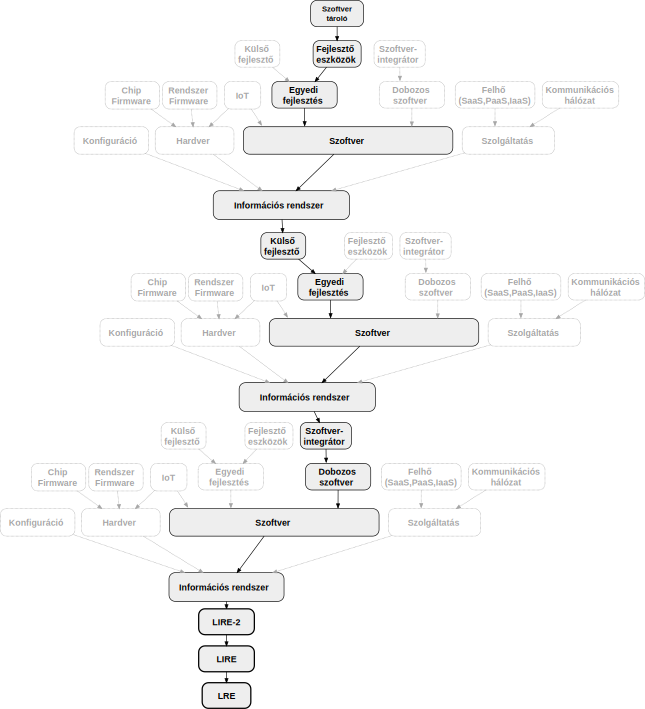
\includegraphics{ábrák/FLOSS_hatáspontjai_example.pdf}
\caption{Egy lehetséges FLOSS belépési pont (szerkesztette a
szerző)}\label{fig:FLOSSHatuxe1sExp}
}
\end{figure}

Mint látható, a szoftveripar jelen fejlettségi szintje mellett a FLOSS
számtalan, nem triviális belépési ponttal rendelkezhet, ráadásul ezek a
pontok többszörösen visszacsatolásokon keresztül bonyolult függőségi
hálózatot alkothatnak. Könnyen előfordulhat, hogy a LIRE biztonsági
szintjét egy látszólag független, távoli folyamat befolyásolja. Ilyen
lehet például egy másik, a vizsgált LIRE tekintetében kiemelt
fontosságúnak tekintett LIRE rendszer információs rendszerében használt
dobozos szoftver, amelynek fejlesztése során a gyártó egyik
beszállítójának egyedi szoftverében olyan nyílt forrású
szoftverforrásokat használnak fel, amelyek függőségei közt egy hibás
komponens található (\ref{fig:FLOSSHatuxe1sExp}. ábra).

Intuitív módon azt várhatnánk, hogy minél messzebb esik a sérülékenység
a végfelhasználás helyétől, annak veszélyessége arányosan csökken,
sajnos azonban általában ennek éppen az ellenkezője az igaz. A
sérülékenység szempontjából teljesen mindegy, hogyan került a
rendszerbe, kizárólag az számít, hogy jelen van és kihasználható.
Ugyanakkor a többszörös áttétel jelentősen lelassíthatja a javítások
végigfutását a rendszeren, következésképpen a támadáshoz már nem
szükséges zero-day\footnote{Bejelentetlen, javítással még nem rendelkező
  sérülékenység} sérülékenység, az egyébként már meglévő javítások a
rendszer tehetetlensége miatt csak jóval később kerülnek bele a
felhasznált szoftverbe.

\hypertarget{sec:ICS}{%
\subsection{OT/ICS rendszerek}\label{sec:ICS}}

Igaz ugyan, hogy az utóbbi években egyértelmű konvergencia figyelhető
meg az Information Technology (IT) és Operational Technology (OT) terén
-- amivel árhuzamosan a FLOSS hatásmechanizmusa is egyre inkább hasonlít
a két területen -- de nem lehet figyelmen kívül hagyni, hogy az ipari
vezérlőrendszerek (továbbiakban ICS\footnote{Industrial Control Systems,
  azaz ipari irányítási rendszerek}) mind teljesítménybeli, mind
megbízhatósági kritériumaikban más követelményeket támasztanak mint a
hagyományos IT megoldások. Másrészről, azok a lehetséges intézkedések,
amelyek működőképesnek bizonyulhatnak az IT területén, korántsem biztos,
hogy alkalmazhatók az OT specializált, gyakran fizikailag is
elkülönített környezetében {[}44{]}.

Az ICS rendszerek direkt fizikai hatást gyakorolhatnak a környezetükre,
így az IT rendszerekkel ellentétben, közvetlen potenciális veszélyt
jelenthetnek az egészségre vagy fizikai biztonságra. Teljesítményüket
tekintve általában alapkövetelmény hatékonyság, megbízhatóság, a valós
idejű vagy közel valós idejű működés, következésképpen a védelmi
intézkedések tervezésénél is más súllyal esnek latba ezek a kritériumok.
Az ICS rendszerek azonnali és magas rendelkezésre állást igényelnek, így
míg IT esetében a biztonságot általában a bizalmasság, sértetlenség és
rendelkezésre állás hármasával jellemezzük, OT esetében a sértetlenség
és bizalmasság csak a rendelkezésre állás után következik {[}45{]}.

Az OT fogalma alá tartoznak mindazon számítási rendszerek amelyek ipari
műveleteket vezérelnek. Az ICS ernyőfogalma alá tartoznak a
SCADA\footnote{Supervisory Control and Data Acquisiton} és
DCS\footnote{Distributed Control Systems} rendszerek (lásd
\ref{fig:ICS}. ábra). Az előbbiek elsődleges célja az adatgyűjtés a
távoli terminálegységeken (RTU) keresztül, amelyek a központi
vezérlőrendszerbe jutva általában grafikus reprezentációval segítik a
magas szintű döntéseket. Az utóbbi, DCS folyamatvezérlő rendszerek
szinte mindig helyben működnek, vezérlőket, érzékelőket, aktuátorokat
kötve össze közös rendszerré. Az adatgyűjtés és vezérlési folyamatok ez
esetben elosztott központi egységeken futnak, amelyek többnyire a
perifériák környezetében helyezkednek el. Elméletben valamennyi ICS
rendszer lehet nyílt forrású, vagy tartalmazhat nyílt forrású
komponenst, ide értve az ember-gép kommunikációt megkönnyítő (HMI) vagy
az alacsony szintű direkt elektronikai vezérlést végző PLC\footnote{Programmable
  Logic Controller} elemeket is.

\begin{figure}
\hypertarget{fig:ICS}{%
\centering
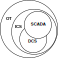
\includegraphics{ábrák/OT-ICS-SCADA.pdf}
\caption{Ipari automatizálás alapelemei (Saját szerkesztés {[}45{]}
nyomán)}\label{fig:ICS}
}
\end{figure}

Korábban az IT és OT rendszerek meglehetősen eltérő szerepet töltöttek
be a szervezeten belül, ennek megfelelően külön is kezelték őket. Az ICS
rendszereket hagyományosan specializált hardver megoldások és üzleti
(zárt forrású) szoftver jellemezte. Telepítésük gyakran önálló jellegű
és általában gyártóspecifikus üzleti kommunikációs protokollt használ.
Napjainkban azonban a gyártási és üzemeltetési költségek
minimalizálására való törekvés valamint a termelékenység növelésének
igénye folytán a ICS gyártók egyre gyakrabban alkalmaznak általánosan
használt hardver és szoftver megoldásokat. A konvergencia kétségtelenül
költséghatékony és jelentősen megnövelheti valós idejű
információáramlást, ugyanakkor az ICS egyben sérülékennyé is válik
mindazon káros hatásokkal szemben amelyek korábban elsősorban az IT
rendszereket jellemezték. A IoT rendszerek népszerűségének növekedésével
ez a folyamat tovább erősödhet.

A konvergencia egyúttal a nyílt forrású fejlesztések térhódítása előtt
is megnyitja az utat. Az ipari automatizálás területén isjelentkező
szabványosítási törekvések -- például az gép-gép kommunikációt
egységesítő OPC Unified Architecture (OPC UA) protokoll megjelenése --
lehetővé teszi a nyílt forrású rendszerek egyszerű illesztését az ICS
komponensekhez. A SCADA rendszerek területén egyre népszerűbb a web
alapú megjelenítés, ezen a területen pedig beágyozott Linux rendszerek
régóta költséghatékony, megbízható és közkedvelt eszköznek számítanak
{[}46{]}. A nyílt forrású rendszerek biztonsági megoldásként történő
felhasználása is egyre gyakoribb. A Linux iptables (azaz napjainkban már
inkább nftables) tűzfala jól használható az ICS rendszerek
határvédelméhez {[}47{]}, valamint a SCADA rendszerek védelme is
elképzelhető nyílt forráskódú alapokon {[}48{]}. A nyílt forrású SCADA
rendszerek teljesítmény terén nem térnek el jelentősen a zárt
forrásúaktól, ugyanakkor általában könnyebben alakíthatók és
platformfüggetlenek {[}49{]}.

Tekintettel arra, hogy a DCS rendszereket mind a mai napig többnyire
kulcsrakész, telepített megoldásként szállítja a gyártó {[}50{]}, ebben
az esetben a nyílt forrás közvetlen megjelenésének valószínűsége
csekély, ugyanakkor számolni kell azzal, hogy a gyártó maga belsőleg
felhasznál ilyen komponenseket. A \ref{sec:ELLENINT}. fejezetben
meghatározott ellenintézkedések korlátozottan érvényesek, lényegében a
zárt forrású IT rendszerekkel azonos módon kezelendők.

A PLC rendszerek napjainkban döntő részt üzleti megoldások, bár léteznek
nyílt forrású PLC rendszerek is, ilyen például az OpenPLC\footnote{https://openplcproject.com/}.
Az otthoni automatizálás és hobbielektronika széleskörű elterjedésével
ezek a rendszerek egyre nagyobb piachoz jutnak, a kiberháborús
fenyegetettség és a bizalmatlanság erősödésével megnövekedhet a
jelentőségük. Egyelőre azonban jelentőségük alacsony, ezért az
\ref{sec:ELLENINT}. fejezetben tárgyalt ellenintézkedések többsége nem
értelmezhető esetükben.

A SCADA rendszerek az IT rendszerekkel azonos szempontok szerint
elemezhetők, szem előtt tartva természetesen a rendelkezésre állással és
megbízhatósággal szemben támasztott eltérő kritériumokat. Az azonos
kezelést az indokolja, hogy ma már léteznek nyílt forrású SCADA
rendszerek, amelyek adott esetben nyílt forrású operációs rendszeren
futnak és a IT rendszerek által is használt hálózatot használják
adatcserére.

\hypertarget{irodalomkutatuxe1s}{%
\section{Irodalomkutatás}\label{irodalomkutatuxe1s}}

A KC-1 kutatási cél eléréséhez Petersen és társai által javasolt
Systematic Mapping Study módszertanát alkalmaztam, amely jól
használható, elterjedt módszer a szoftverfejlesztés terén felmerülő
osztályozási problémák kezelésére és a téma struktúrálására {[}22{]}.

A Systematic Literature Review (SLR) módszerével ellentétben a
Systematic Mapping Study (SMS) a témákra bontott tudományos bizonyítékok
elérhetőségére koncentrál, kevésbé érzékeny a precízen megfogalmazott
keresőkérdésekre és nem igényli a publikációk minőségének értékelését
{[}51{]}. Egy szélesebb terület átfogó elemzésére az SMS megfelelőbb
eszköz, ugyanis segítségével hatékony képet alkothatunk az egyes
részterületek kutatottsági állapotáról és módszereiről.

A Systematic Mapping Study tervezésének vázlatos lépései az alábbiak:

\begin{enumerate}
\def\labelenumi{\arabic{enumi}.}
\tightlist
\item
  téma és kérdésfelvetés;
\item
  kutatási terv, források és keresőkifejezés meghatározása;
\item
  tanulmány kiválasztási és elutasítási kritériumok meghatározása;
\item
  adatgyűjtés;
\item
  adatelemzés;
\item
  eredmények előállítása.
\end{enumerate}

A fejezetben csak az irodalomkutatás vázlatát és következtetéseit
ismertetem, az eredmények, analízis és a részletes módszertan a
\ref{sec:IKUT}. függelékben található.

\hypertarget{kutatuxe1si-cuxe9l-uxe9s-muxf3dszertan}{%
\subsection{Kutatási cél és
módszertan}\label{kutatuxe1si-cuxe9l-uxe9s-muxf3dszertan}}

A teljes kutatómunka kérdésfelvetésével összhangban az SMS tanulmány az
KC-1.1 kutatási célt hivatott megvalósítani, azaz felméri, hogy a FLOSS
egyes hatásai mennyire kutatottak a különféle területeken. Az SMS
tanulmány által összegyűjtött anyagok egyúttal a jellegzetességek
rendszerezésének (KC-1.2) és a sajátosságok meghatározásának (KC-1.3)
alapját is képezik.

A kutatási célkitűzés további bontásával az alábbi részcélokat
határoztam meg:

\begin{itemize}
\tightlist
\item
  A nyílt forrású szoftverek biztonsággal kapcsolatos egyedi
  sajátosságainak meghatározása.
\item
  A kutatói közösség milyen súllyal foglalkozik az egyes
  sajátosságokkal?
\item
  Milyen típusú kutatásokat végeztek a témában?
\item
  Milyen témákkal foglalkoznak a kutatók?
\item
  A jelenlegi FLOSS biztonsággal kapcsolatos eredmények milyen
  biztonsági hatásokat azonosítanak?
\end{itemize}

A kereséseket négy nagy digitális könyvtár -- IEEE Digital Library, ACM
Digital Library, ScienceDirect és SpringerLink felhasználásával
hajtottam végre, amelyek vélhetően megfelelően lefedik a területen folyó
mértékadó kutatásokat. Az adatgyűjtésben valamennyi, tehát nem csak a
szabadon elérhető (Open Access) publikációk kerültek bele, ami
sajnálatos módon csökkenti a kutatás reprodukálhatóságát, de úgy véltem,
a szabadon elérhető művek relatív alacsony száma miatt a területet csak
a teljes anyagmennyiséggel lehet megfelelően lefedni.

A kutatásban alkalmazott protokoll (szűrési és kihagyási kritériumok) a
függelékben megtalálhatók. A kiválasztást duplum-ellenőrzésre követte.
Az adatgyűjtés eredményét SQLite adatbázisban rögzítettem, a szűréseket
és vizualizációt saját fejlesztésű szoftverrel végeztem el. A keresés,
szűrést, duplumellenőrzést követően összesen 934 publikációt elemeztem.

A publikációk rendszerezése érdekében hat kvalitatív és egy kvantitatív
(év) osztályt vezettem be. Az osztályozás kategóriáit részben korábbi
tapasztalatok, részben egy 50 elemű pilot halmaz segítségével határoztam
meg. Az elemzésben a következő kategóriákat használtam: ``kutatás
típusa'', ``biztonsági kategória'', ``hozzájárulás'', ``sajátosság
kategória'', ``téma'' és ``tudományos módszertan''.

Az osztályok kategória-cimkéit, részletes elemzést és a grafikus
eredményeket a függelék tartalmazza.

\hypertarget{uxf6sszefoglaluxf3-analuxedzis}{%
\subsection{Összefoglaló
analízis}\label{uxf6sszefoglaluxf3-analuxedzis}}

Megállapítottam, hogy a leginkább kutatott FLOSS sajátossági kategória a
fejlesztési módszertan különbsége. Természetesen ebből nem következik,
hogy a biztonságra ez a sajátosság gyakorolja a legnagyobb hatást, de --
legalábbis a publikációk száma alapján -- ez a kérdés a legjobban
kutatott, itt várható stabil eredmény, a lehetséges biztonsági problémák
legnagyobb lefedettsége.

A vizsgált időszakban a tudományos közösség a probléma megismerésére,
megértésére koncentrál. Erre utal a tájékozódó módszerek (esettanulmány,
felmérés) dominanciája és az uralkodó publikáció típusok (tapasztalatok,
értékelések, feltérképezés) száma szemben az elméleti munkák alacsony
részarányával.

Úgy találtam, hogy a javasolt módszerek száma egyenletes, bár a
forrásadatok elérhetősége és a módszertan eloszlása kimutathatóan
kiegyensúlyozatlan. A kutatói közösség valamennyi FLOSS területet
fontosnak tartja, megoldási javaslatokkal is él, ám megfelelő
alapkutatások híján bizonyos területeken igen nehéz tudományos
eredményeket felmutatni.

A FLOSS biztonsági kérdéseivel kapcsolatos kutatások többnyire
szoftverminőség-vizsgálattal kapcsolatos esettanulmányok és
adatelemzések. A tudományos közösség a szoftverminőség-vizsgálatra és
sérülékenységekre koncentrál, egyéb biztonsági területek (pl. tesztelés,
életciklus menedzsment, konfiguráció menedzsment stb.) meglehetősen
alacsony. Megállapítom, hogy a FLOSS biztonsági kérdéseinek kutatása a
vizsgált időszakban egyoldalú és néhány részterületre fókuszált.

A szűrés és elemzés során számos olyan új sajátosság is felmerült, amely
a kutatás korábbi szakaszából származó rendszerezésbe nem volt
beilleszthető. Ezeket a jellemzőket a taxonómia bővítésével kezeltem,
illetve felvételre kerültek a biztonsági hatásokat nyilvántartó
adatbázisba. Ilyen, korábban rendszerezetlen jelentősebb sajátosság volt
például a preprocesszor kapcsolók használatának lehetősége, a fejlesztői
függetlenség és az ezáltal kialakuló fejlesztői befolyás kérdése, a
Trusted Platform technológiákkal való esetleges inkompatibilitás kérdése
illetve az egyszerű hozzáférhetőség folytán kialakuló kódmásolás
(kódbeszivárgás) problémaköre. A felderített biztonsági hatásokkal
részletesen a 2. fejezetben foglalkozom.

\hypertarget{ruxe9szkuxf6vetkeztetuxe9sek}{%
\section{Részkövetkeztetések}\label{ruxe9szkuxf6vetkeztetuxe9sek}}

A KC-1 célkitűzés keretében a LIRE és a FLOSS elemek kapcsolatát
vizsgáltam. Megállapítom, hogy a LIRE többszörös függősége és a FLOSS
bujtatott jelenléte folytán a biztonságra gyakorolt hatás rendkívül
összetett, elméletileg tetszőleges számú közvetítőn keresztül is
létrejöhet. A feltörekvőben lévő felhő és IoT technológiák terjedésével
a helyzet különösen kiéleződhet, tekintettel e területek jelentős
(gyakran rejtett) FLOSS felhasználására.

A LIRE direkt FLOSS kitettsége az alábbi négy szint valamelyikén
valósulhat meg:

\begin{itemize}
\tightlist
\item
  \textbf{I. típus}: A szervezet üzleti termékként, viszonteladótól
  szerzi be a nyílt forrású szoftvert avagy hardver komponensként,
  nagyobb szoftvercsomag részeként illetve önálló megoldásként
  alkalmazza azt.
\item
  \textbf{II. típus}: A szervezet közvetlenül a fejlesztőközösségtől
  szerzi be a szoftver terjesztésre szánt változatát, csomagkezelő
  rendszeren keresztül vagy direkt módon, általában bináris formában.
\item
  \textbf{III. típus}: A szervezet saját belső előírásai szerint
  fordítja le a FLOSS termék stabil vagy fejlesztői változatát az
  eredeti forráskód felhasználásával. A szervezet ez esetben képes a
  fordítási opciók illetve akár a forrás módosítására.
\item
  \textbf{IV. típus}: A szervezet direkt vagy közvetett módon részt vesz
  a fejlesztésben, saját fejlesztési ágat vezet, egyedi módosításait a
  szülő projektbe visszavezeti vagy folyamatosan karbantartja.
\end{itemize}

Az áttételes hatás tényleges megvalósulási gyakoriságának vizsgálata
sajnos objektív akadályokba ütközik, tekintettel a LIRE pontos
felépítésének érzékeny és minősített voltára. Hazai LIRE rendszerek
vezető üzemeltetőivel\footnote{Dr.~Bognár Balázs tü. ezredes, Horváth
  Ferenc tü. alezredes (BM OKF, informatikai főosztály), Dr.~Futó Iván
  (NAV főkoordinátor, Vám- és Pénzügyőrség informatikai integrációjának
  vezetője), Orosz Attila (Földhivatal, inf. főosztály).} folytatott
írásbeli és személyes találkozók keretében meggyőzödhettem róla, hogy a
kutatásban feltárt hatáspontok legalább egy része mindenképpen valós
lehetőség, továbbá a \ref{sec:FLOSSBELSO}. fejezetben bemutatok néhány
konkrét példát is.

A KC-1.1 célkitűzésnek megfelelően megállapítottam, hogy a tudományos
közösség jelentős túlsúllyal foglalkozik a FLOSS fejlesztési módszertan
kérdéseivel, míg más aspektusok (biztonság, megfelelőség, életciklus
menedzsment) kevésbé kutatottak. A biztonsági kérdéseket is érintő
munkák döntő részben a nyílt forrású termékek
szoftverminőség-vizsgálatára szorítkoznak. A könnyen hozzáférhető
forráskód okán gyakran szerepelnek kutatások adatforrásaként, de a
nyíltság konkrét hatásainak vizsgálatával a publikációk általában nem
foglalkoznak.

A javasolt módszerek egyenletes eloszlást mutatnak a sajátosságok
tekintetében, azaz a kutatói közösség valamennyit fontosnak tartja,
ugyanakkor empirikus adatok és alapkutatási eredmények első sorban a
nyílt forrású fejlesztés területén állnak rendelkezésre, ezért az
eredmények döntő része is ide koncentrálódik.

Megállapítottam, hogy a gazdasági hatással, tudati dimenzióval,
terméktulajdonságokkal kapcsolatos jellemzők vizsgálatához szükséges
adatot jelenleg kizárólag szűk területre koncentrálódó (nem
reprezentatív) felmérésekből lehet gyűjteni vagy egyáltalán nem áll
empirikus eredmény rendelkezésre és csak szakértői véleményekre
támaszkodhatunk.

A kutatás első fázisában többszöri finomítással létrehoztam a FLOSS
sajátosságok egy lehetséges rendszertanát (\ref{fig:FLOSSSaj} ábra)
amely megfelel a KC-1.2 célkitűzésnek. Ezt a rendszertant alkalmazom az
következő fejezetekben.

Megállapítom, hogy a FLOSS mint jelenség LIRE-re gyakorolt hatásainak
vizsgálatához semmiképpen sem elegendő a LIRE elsődleges rendszereinek
vizsgálata. A FLOSS esetleges sérülékenységei akkor is jelentős hatást
gyakorolhatnak a LIRE komponenseire, ha az információs rendszer
közvetlenül (papíron) semmilyen FLOSS megoldást nem használ.

\hypertarget{sec:FLOSSBELSO}{%
\chapter{Belső sajátosságok}\label{sec:FLOSSBELSO}}

\hypertarget{fejlesztuxe9si-folyamatok-fs-f}{%
\section{Fejlesztési folyamatok
(FS-F)}\label{fejlesztuxe9si-folyamatok-fs-f}}

Az üzleti szoftverfejlesztési folyamatok nem igazán illeszkednek a
klasszikus nyílt fejlesztési közösségekre {[}52--54{]}, a két modell
ugyanis kulturálisan különbözik. Míg az zárt modell a fejlesztők
ellenőrzésén, fix ütemezése és minőségbiztosítási elveken
alapul{[}55{]}, a nyílt modell a szabadságot, az önszerveződést és az
innovációt helyezi előtérbe. Napjainkban a helyzet persze már nem ilyen
egyértelmű, hiszen a klasszikus nyílt modell mellett egyre gyakrabban
találkozunk cégirányítás alatt álló vagy szponzorált FLOSS projektekkel,
amely a delegált fizetett fejlesztőkön keresztül a hagyományos
szoftverfejlesztés módszertanát vegyíti a közösségi modellel {[}36,
56{]}. Sőt, ez a folyamat kétirányú, az üzleti fejlesztésben is
terjednek a nyitottabb módszerek (Scrum, Kanban) valamint egyre
népszerűbb a nyílt modell elveit használó Inner Source
irányzat{[}57--59{]} valamint a nyílt forrás folyamatos
fejlesztés-fordítás-tesztelés ciklusát átvevő Continous Integration (CI)
módszertan is {[}60{]}. Az alábbiakban elsősorban a klasszikus önkéntes
nyílt modell jellemzőre koncentrálok, hiszen innen ered a FLOSS modell
eltéréseinek döntő része.

A nyílt modellt gyakran támadják amiatt, hogy a hagyományos
szoftverfejlesztés számos fontosnak tartott eleme, mint a formális
követelmény-specifikáció, architektúra dokumentáció vagy
minőségbiztosítási szabályozás messze elmarad az üzleti világban elvárt
szinttől illetve sok esetben teljesen hiányzik. Előfordul, hogy a
rendszer biztonsági architektúrális leírása -- ha létezik -- csak
elszórt dokumentációkból gyűjthető össze és nincs szervezett biztonsági
képzés {[}61{]} a számos fiatal fejlesztő és az ellenőrzés hiánya
folytán a fejlesztők biztonságtudatossága nem mindig megfelelő {[}62{]}.
A hibrid vagy szponzorált nyílt fejlesztési közösségek üzleti szemlélete
segít kiküszöbölni a hiányosságok egy részét{[}63{]}, ehhez azonban a
szervezeteknek megfelelő befolyást kell szereznie a projekt felett.
Csakhogy a túlzott befolyás nem előnyös, elriasztja a fejlesztők egy
részét {[}64{]} illetve extrém esetben forkot kényszeríthet ki (pl.
MariaDB vs.~Oracle MySQL). A fork egyik gyakori célja a
projektmenedzsment megváltoztatása {[}65{]}.

Valójában a tradicionális nyílt közösség önmagában is képes a zárt
modellel azonos minőségű kódot előállítani, az eredmény és a növekedés
üteme általában nem lesz látványosan jobb, de rosszabb sem {[}66, 67{]}.
Ez a teljesítmény azonban egyáltalán nem a véletlennek vagy a zseniális
elméknek, hanem egy eltérő, de éppoly jól szervezett és fegyelmezett
módszertannak {[}68{]} köszönhető amely néhány tekintetben hasonlít a
zárt modellből ismert Agilis Szoftverfejlesztés\footnote{Angol nevén
  Agile Software Development, szoftverfejlesztési módszerek egy
  csoportja, ahol a megoldásokat együttműködés révén önszerveződő
  multifunkcionális csoportok valósítják meg.} módszertanához ám nem
azonos azzal{[}69{]}.

A szoftverfejlesztés hagyományos pillérei a követelmény-specifikálás,
tervezési szakasz, a programfejlesztés, tesztelés, kiadás, karbantartás
és folyamatot összefogó minőségellenőrzés. A nyílt modell ezeket gyors
kiadási ciklusok alkalmazása mellett egymással párhuzamosan végzi, az
egyes folyamatok nem is különülnek el élesen.

\hypertarget{sec:FS-F-K}{%
\subsection{Követelmények meghatározásának eltérései
(FS-F-K)}\label{sec:FS-F-K}}

Több publikációban is megjelenik a FLOSS és üzleti projektek
követelmény-rendszere közötti eltérés kérdése. Egyértelmű különbség
mutatkozik a projektek magasabb rendű céljai, e célok megfogalmazásának
mikéntje, a célok felhasználó-centrikussága és a célok elérésének
határideje terén. Az alábbiakban ezeket a tényezőket mutatom be.

\emph{Funkcionális követelmény meghatározás eltérései.} Üzleti
környezetben általában megengedhetetlen a célok hanyag megfogalmazása,
míg egy FLOSS projekt megelégedhet vázlatos funkcionális
követelmény-specifikációval {[}70, 71{]} ami csak idővel tisztul le
{[}72{]} megfelelő mértékben. Más részről nyílt modell gyakran
emlegetett jellegzetessége miatt -- nevezetesen, hogy a fejlesztők
egyben felhasználók is -- a funkcionalitás stratégiai céljai már a
kezdetektől sokkal tisztábbak, nem a fejlesztő és a vásárló hosszú és
nehézkes egyeztetése során jönnek létre {[}73{]}. A FLOSS fejlesztésben
tehát az informális célok általában világosak, de nem jellemző viszont a
mérhető célok definiálása {[}74{]} a követelmények kidolgozása során. A
klasszikus FLOSS projektben általában nincsen formális
követelményrendszer, a fejlesztési irányokat közösségi vita dönti el
{[}75--77{]}, ezzel ellentétben az üzleti irányítású közösségekben (pl.
Android) a célok többnyire világosak, meghatározásuk semmiben nem tér el
az üzleti változatokétól, ami nem véletlen, hiszen itt az irányítás egy
piaci szereplő kezében van {[}78{]}.

\emph{Időbeli célok eltérései.} A FLOSS projekteket nem motiválja az
időben történő piacra kerülés. Ez egyrészt biztonsági szempontból
kedvező, hiszen nincs határidő nyomás a fejlesztőkön, felhasználói
részről viszont kedvezőtlen, hiszen esetleg hosszú időn keresztül nem
jutunk hozzá a kívánt funkcióhoz{[}79{]}.

\emph{Felhasználó centrikusság.} A FLOSS fejlesztés alapvetően nem
felhasználó-centrikus. Amennyiben kevésbé technikai felhasználók (azaz a
fejlesztők halmazán kívül esők) igényelnek valamilyen funkciót, az vagy
bekerül a specifikációba vagy nem, szabad kapacitástól függően, ami
jelentős különbség ez az üzleti világhoz képest, ahol a felhasználói
igény kielégítése a fejlesztés elsődleges iránya. A nyílt modellben nem
cél a vásárló elégedettsége {[}80, 81{]}, az igényfelmérést és
követelmények meghatározását programozók és nem erre szakosodott
szakemberek végzik {[}74{]} és általában hiányzik az igényekre vonatkozó
komplex adatgyűjtés {[}82{]} is. A felhasználók brainstorming jelleggel,
levelező listákon és fórumokon keresztül adhatnak hangot igényeiknek,
bizonyos mértékig részt vállalva a projekt tervezésében (legalábbis
nagyobb mértékben mint a zárt modell esetén {[}83{]}).

Ezt a tervezési módszertant számtalan zsákutca, elvetélt változat és
igen lassú haladás jellemzi {[}84, 85{]} így hatékonysága és
eredményessége megkérdőjelezhető {[}86, 87{]}, ugyanakkor igaz, hogy
ezáltal egy sokkal nagyobb halmaz -- a felhasználói bázis jelentős része
-- vesz részt az innovációban {[}88{]}. A funkcionális igény lassú
teljesülése LRE rendszerek esetén problematikus lehet, különösen ha ez a
hiányzó igény pont a biztonság. A felhasználók alacsony érdekérvényesítő
képességére vezethető vissza a FLOSS használhatóságbeli problémái
{[}89{]} hiszen a technikailag képzetlenebb felhasználó és a fejlesztést
irányító fejlesztő-felhasználó számára a jó használhatóság merőben mást
jelenthet (felhasználói interfész kidolgozottsága, beállítási
lehetőségek egyszerűsége, beépített segítség stb. vonatkozásában).

Többnyire az üzleti termékek felhasználóinak sincs lehetőségük
beleszólni a fejlesztésbe, de általában bíznak benne, hogy a piaci végül
a megfelelő irányba tereli a fejlesztést{[}90{]}. FLOSS esetén az lesz
az irány, amit a ``látnok'' kijelöl, vagy amit a többség megszavaz (lásd
\ref{sec:FS-K-Sz}). Emiatt az üzleti felhasználóknak nagyon fontos, hogy
megfelelő lobbierővel rendelkezzenek, amit támogatással, de leginkább a
közösség munkájában való részvétellel érthetnek el. Nem véletlen, hogy
az igazán nagy piaci értéket képviselő FLOSS projektekben (Linux, cloud
technológiák területe) általában szerepet vállalnak az technológiát
felhasználó nagyvállalatok illetve -- többnyire konzorcium formájában --
egész egyszerűen átveszik annak vezetését.

Biztonsági szempontból a felhasználó-centrikusság és a piacorientáltság
hiánya nem feltétlen hátrány. A felhasználók igazoltan hajlamosabbak
fizetni az érdekes funkciókért mint a biztonságért. Egy biztonsági
hiányosságokkal terhelt de funkciógazdag termék jobban eladható, mint
egy biztonságos, ám funkciószegény változat, még akkor is, ha a hiányzó
funkciókat a felhasználók valójában nem is használják {[}91{]}.

\emph{Hosszú távú tervezés .} A FLOSS közösség alapvető stratégiai célja
nem a profit, az időben való piacra kerülés vagy egy kitűzött
specifikáció megvalósítása, hanem az együttműködés egy ötlet körül
{[}92--94{]}. A piaci céloktól való függetlenség pozitív hozadéka az
jobb hardver kompatibilitás. Egy-egy hardver támogatottsága nem tűnik el
pusztán azért, mert már nem gazdaságos azt fenntartani{[}95{]}. Egy
Linux rendszert mind a mai napig le lehet fordítani i386-os
architektúrán, Gravis Ultrasound támogatással, holott ezt a hardvert
lassan már csak múzeumokban találjuk meg.

A fejlesztés hangsúlya általában az innováción és nem a stabilitáson van
{[}96, 97{]}, bár ezt a problémát a legtöbb projekt stabil, teszt és a
legfrissebb ``bleeding edge'' verziók használatával igyekszik enyhíteni.

A célok és követelményrendszer megfogalmazásának fent említett eltérése
a FLOSS idealista fejlesztőközössége és a cégek vezetőinek gondolkodási
különbségeire vezethető vissza. A cégvezetők gyakran nem kevés
gyanakvással tekintenek a FLOSS projektekre az üzleti gondolkodástól
elütő idealizmusuk miatt {[}98{]}.

A követelményrendszer különbözőségének kezelésére esetleg megoldást
jelenthetnének a már ma is létező szabadúszó licit\footnote{Az un.
  freelancing vagy microjob platformokon különféle részfaladatokra
  jutalmat kitűzve szabadúszókat bérelhetünk. Ilyen platform a
  Freelancer.com, Truelancer, Upwork, Guru, Zeerk.} vagy crowdsourcing
rendszerekhez hasonló platformok kialakítása, ahol a fejlesztésben részt
nem vállaló felhasználók a hiányzó funkciókra vagy magára a projektre
licitálhatnának. Ez egyúttal a FLOSS fejlesztések finanszírozási
problémáin is segítene. Az ilyen irányú próbálkozások a FLOSS esetében
egyelőre gyerekcipőben járnak (élő példa többek közt az IssueHunt vagy a
BountySource {[}99{]}), egy jól működő modellhez a technikai lehetőségen
túl valószínűleg mélyreható társadalmi, hozzáállásbeli változások
szükségesek.

Jelenleg a projekt céljainak befolyásolásra az egyetlen gyakorlatban is
kivitelezhető megoldás úgy tűnik a projektben való részvétel {[}100{]}.

\hypertarget{sec:FS-F-P}{%
\subsection{Tervezés (FS-F-P)}\label{sec:FS-F-P}}

Általános nézet, hogy a FLOSS projektek nem alkalmaznak formális
tervezési módszereket, sőt egyes esetekben a tervezők egyenesen
másodrendű állampolgárok a közösségben{[}101{]}. A projektek gyakran
azonnal programozással indulnak, átfogó tervek csak a fejlesztés
folyamán vagy egyáltalán nem születnek{[}74{]}. A modellek, különösen a
dokumentált modellek használata ritka {[}102{]}, ami problémát jelenthet
ha a projektet átlátó régi fejlesztők helyére újaknak kell lépniük,
hiszen a betanulási idő igen hosszúra nyúlhat {[}103{]}. A helyzetet jól
jellemzi, hogy a GitHub projektek mindössze 0.28\% tartalmaz
UML\footnote{Unified Modeling Language, általános célú, elterjedt
  modellező nyelv a szoftverfejlesztés területén.} diagrammot és ezeknek
is csak egyharmada tartalmaz egynél többet {[}104{]}.

A közösség alapvetően projekt és nem szervezet központú{[}105{]} a
fejlesztők javításokról vagy funkciókról blogolnak, menedzsment
kérdésekről csak egészen elvétve esik szó {[}106{]}. Jobbára nincs
definiált módszertan {[}53, 71, 74{]}, a fejlesztési stratégia
dokumentációja többnyire kimerül valamilyen programozási stílus
útmutatóban (ami viszont igen gyakori) {[}107{]}. Ha van is formális
követelményrendszer, kisebb projektekben ritkán tartják be és még
ritkábban ellenőrzik {[}108{]}.

Az önállóan választott feladatok, a szerepkörök egybemosódása kockázatot
hordozhat. Nem érthet mindenki mindenhez. A kivitelező szakemberek nem
feltétlen képesek jó modelleket alkotni, ahogy a modellező szakember sem
biztos, hogy képes jól végrehajtani azt {[}109{]}. A FLOSS közösségek
ritkán fogalmaznak meg formális biztonsági követelményeket, a meglévő
biztonsági minősítő módszerek is stabil tervezési és fejlesztési
folyamatokat feltételeznek, ami megnehezíti a FLOSS biztonsági
tanúsítását {[}75{]}. Minthogy a megszokott módszerek nehezen
használhatók a tanúsítást a kód és a metaadatok elemzésével lehet
elvégezni {[}110{]}.

Az tervezésre jellemző a nagy fokú modularitás és a komponensek extenzív
használata {[}52, 111, 112{]} amit az adapter pattern gyakori jelenléte
is jelez {[}113{]} ugyanakkor jelentős komplexitást vezet be és
verzió-frissítési problémákhoz vezethet. A FLOSS általában valóban
modulárisabb mint a zárt modell {[}80{]} amire szükség is van, hiszen a
nagy számú fejlesztő csak így tud hatékonyan együtt dolgozni
elfogadhatatlanul magas integrációs és koordinációs költség
nélkül{[}114, 115{]}. Az újonnan érkezők az őket érdeklő részre tudnak
fokuszálni, anélkül hogy a többiek munkáját zavarnák {[}53{]}. A
modularitás további előnye, hogy egyetlen jól meghatározott feladatot
végző könyvtárban könnyebb megtalálni a hibát, mint egy komplex
rendszerben{[}116{]}. A modularitás mérhető {[}117{]}, a mérőszámok
segítségével következtetéseket vonhatunk le a projekt sikerességére
vonatkozóan.

A kódbázisban erős kód-coupling\footnote{Coupling: a programkódban
  található objektumok függőségét mutató mérőszám. Az erősen függő
  (highly coupled) kód nehezen módosítható, mert a változtatás sok más
  objektum működésére hatással lehet.} figyelhető meg, ami részben a
központi tervezés és modellező eszközök hiányára vezethető vissza
{[}118{]} részben szándékos módszertani következmény. A nyílt modellre
általában, a Linux disztribúciók esetében pedig különösen igaz, hogy
nagyon sok a függőséget tartalmaznak{[}119{]}. A csomagok közötti
bonyolult függőségi rendszer ellehetetleníti a különböző kiadások
közötti kompatibilitást{[}120, 121{]}, az egy adott verzión futó bináris
egyáltalán nem biztos, hogy fut a másikon. (Ugyanez igaz egy szoftveren
belül a komponensek tekintetébe is, igaz ezzel a jelenséggel a
végfelhasználó csak ritkán találkozik). Ennek oka a magas szintű
komponens újrahasznosításban keresendő{[}81, 114, 122{]}. A meglévő
komponenseket (bináris programkönyvtárak vagy osztályok) a teljes
projekt nagyon sok része használja, viszont a komponensből lehetőség
szerint csak egyetlen verziót integrálnak, melynek eredményeképpen jóval
kisebb, konzisztensebb, ugyanakkor az ABI/API\footnote{API: Application
  Program Interface, ABI: Application Binary Interface} eltérések miatt
sokkal kevésbé kompatibilis rendszerhez jutnak. Ebből kifolyólag
egyetlen FLOSS sérülékenységnek igen széles körű hatása lehet {[}123{]}.
A felhasznált nagyszámú komponens következménye, hogy a komponensek
sérülékenységeit is megörökli az új rendszer. A komponensek
sérülékenység eloszlása hasonló mintát mutat mint az azokat felhasználó
projekteké {[}124{]}.

Amikor egy komponens nem illeszkedik tökéletesen gyakran egyszerűen
megváltoztatják{[}125{]} és helyi módosításként kerül a kódbázisba, ami
további hibalehetőséget visz a rendszerbe (a korábban említett hírhedt
openssl sérülékenység is helyi foltként került a disztribúcióba).

A függőségek kérdése azért is nagyon fontos, mert a projektek a
függőségeik közt szereplő komponens-projekteket nagyon ritkán
monitorozzák {[}116{]} és ritkán frissítik {[}126{]}. Kula et al.~4600
GitHub projektre kiterjedő analízise szerint a függőségek több mint
80\%-át nem frissítették, így azok idejétmúltak voltak {[}127{]}. Ebből
viszont az következik, hogy ha egy sokat használt komponensben
sérülékenységet vezetnek be, az nagyon könnyen és észrevétlenül
szétterjedhet, elérve és veszélyeztetve a végfelhasználó rendszereit is.
A csomagfüggőségek tetemes karbantartási költséget jelenthetnek, ugyanis
hatásuk tranzitív módon érvényesül. A frissítések beolvasztásával a
konfliktusok száma nő, tiltásával viszont fontos frissítéseket hagyunk
figyelmen kívül {[}128{]}.

Ezen a problémán igyekeznek segíteni a modern csomagkezelő rendszerek
biztonsági tanusítást végző funkciói, amelyek a telepített csomagok
valamennyi függőségén végighaladva felhívják a figyelmet az ismert
sérülékenységekre. A csomagkezelő rendszerek sajátosságait
\ref{sec:FS-T-M}. fejezetben vizsgálom részletesebben.

\hypertarget{sec:FS-F-M}{%
\subsection{Minőségbiztosítás (FS-F-M)}\label{sec:FS-F-M}}

OSSD esetén többnyire nincs formális minőségbiztosítás {[}129, 130{]} a
kisebb projektek nem gyűjtenek minőségre vonatkozó empirikus
bizonyítékokat{[}74, 131{]}, de alkalmaznak ad hoc megoldásokat és
kódminőséget javító módszereket (code readings, walk through,
refactoring, peer review) {[}81, 107, 132{]}. A kódátnézés módszertana
nagyon hasonlít az üzleti fejlesztési módszertanban alkalmazotthoz
{[}133{]}. Nagyobb projekteknél a minőségbiztosítás gyakran patchelés
alapú fejlesztési megközelítés pótolja, azaz egy adott módosítás halmaz
csak szigorú ellenőrzés és az ellenőrök általi digitális aláírás
megszerzése után kerülhet az upstream\footnote{Általános értelemben
  upstream kódbázisnak nevezzük a projekt által felhasznált külső kódot,
  programkönyvtárakat, modulokat. A verziókezelők esetében azt a verziót
  nevezik upstreamnek, amelyből a szóban forgó változatot készítették
  (forkolták).} kódbázisba{[}134{]}.

A minőségre implicit módon kihatnak pszichológiai tényezők is, hiszen a
nyilvánosságból adódóan a kiadott kódot nagyon sokan látják, a kóddal
kapcsolatos nézeteiket, a szerintük helyes megközelítést kommunikálják
is, ami egyrészt sokat lendít a tanulási folyamaton, másrészt bizonyos
kényszerítő erőt jelent a helyes programfejlesztési módszertan és a
szabványok követésére{[}135{]}. A kód ellenőrzés lefedettségének
növelése a szoftver minőségét és biztonsági szintjét egyaránt erősíti
{[}136{]}.

Bizonyos értelemben a zárt modellben implicit míg nyílt modellben
explicit minőségellenőrzés végezhető. Míg zárt forrás esetén a
minőségbiztosítás elvégzését és szintjét egy tanúsítvány bizonyítja,
azaz elsősorban bizalmi kérdés, a nyílt modellben az elvégzett munka
közvetlen módon, egyértelműen ellenőrizhető és mérőszámokkal
jellemezhető {[}92, 137{]}.

\hypertarget{sec:FS-F-V}{%
\subsection{Kivitelezési szakasz (FS-F-V)}\label{sec:FS-F-V}}

A FLOSS modell sok, hagyományosan elkülönülten kezelt lépést a
kivitelezés során végez. A kivitelezéssel párhuzamosan futnak a béta
tesztek, a tervezés, hibajavítás, más elemek viszont kimaradnak,
általában nem tartják nyilván például a problémák megoldásával járó időt
szemben az üzleti világban megszokott eljárással {[}138{]}. A
hagyományos kivitelezési módszertan valószínűleg nem is igazán működne,
az esetenként több ezres fejlesztőtábor, magas fluktuáció és az
``egyszeri'' fejlesztők miatt. Az átlagos közösségben töltött idő
egészen alacsony is lehet (Android 65 nap, Linux 24-57
nap\footnote{Természetesen vannak állandó fejlesztők is, az átlag az
  egy-két alkalommal hozzájárulók miatt ilyen alacsony.}){[}78{]}

Minthogy a fejlesztés közösségi hozzájárulásokon alapszik, ezeknek a
kódmódosításoknak valahogy be kell kerülniük az upstream kódbázisba. Ez
a folyamat általában szabályozott és gyakran igen komoly
követelményeknek kell megfelelni{[}139, 140{]}:

\begin{enumerate}
\def\labelenumi{\arabic{enumi}.}
\tightlist
\item
  A kódmódosítás halmaznak az aktuális fejlesztői verzióból kell
  származnia és alkalmazkodnia kell a projektben elvárt fejlesztési
  sztenderdekhez.
\item
  A külső féltől származó hozzájárulásokat általában valaki elemzi. E
  lépés célja a megfelelő minőség biztosítása, funkcionális ellenőrzés.
  A kódellenőrzést általában több kis csoport végzi, melyek mindegyike
  egy-egy területre koncentrál {[}141{]}, a jó ellenőr megtalálása nem
  mindig könnyű, ami jelentősen megnövelheti az átfutási időt {[}142{]}.
\item
  A kódot addig módosítják amíg el nem éri a közösség által elvárt
  szintet.
\item
  Ezek után a projekt valamely szenior tagjának jóvá kell hagynia a
  módosítást biztosítva, hogy az új kód hibamentes és teljesíti a
  regressziós teszteket;
\item
  végül a kód integrálásra kerül a kódbázisba.
\end{enumerate}

\begin{figure}
\centering
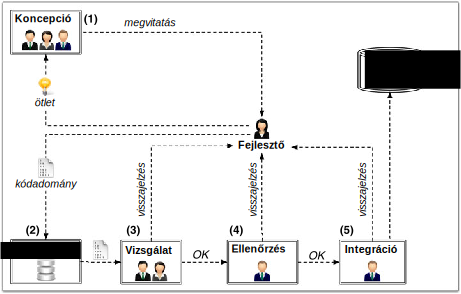
\includegraphics[width=0.78\textwidth,height=\textheight]{ábrák/hozzájárulás-módja-bettenburg_management_2015.pdf}
\caption{Módosítás elfogadásának mechanizmusa OSSD esetén. (Saját
szerkesztés, Bettenburg nyomán {[}78{]})}
\end{figure}

A teljes folyamat elég erőforrásigényes, kivitelezése gyakran meghaladja
a kisebb projektek lehetőségeit, melyeknek így nehézségeket okoz a
hozzájárulások menedzselése {[}78{]}. Ezen a problémán segít a közösségi
fejlesztőportálok (pl. Github) pull request\footnote{közösségi
  fejlesztő-portálokon alkalmazott eljárás, amely formális keretet
  biztosítva leegyszerűsíti a kódelfogadás folyamatát. A kérelmező saját
  kódváltozatából létrehozott módosításkészletet elküldi a projekt
  fejlesztőjének, aki azt soronként átnézheti, a változáskészlethez
  megjegyzéseket fűzhet, módosításokat kérhet, illetve igény szerint
  elfogadhatja azt.} funkciója, amely az elfogadási folyamat
bürokratikus terhét részben leveszi a magfejlesztők válláról
{[}143--145{]}.

Ez a többlépcsős kódelfogadási módszer fontos pillére az kódminőség
biztosításának, ugyanis a tapasztalatlan fejlesztők 2-20x annyi
sérülékenységet vezetnek be mint a tapasztaltabb belső fejlesztők.
Érdekes módon megfigyelhető, hogy a fizetett fejlesztők is nagyobb
eséllyel vezetnek be új sérülékenységet mint a közösség többi tagja
{[}132{]}.

A perifériáról a mag közelébe kerülők ráhatása jóval nagyobb a
projektre. A magfejlesztők változtatásait sokkal nagyobb valószínűséggel
fogadják el és sokkal hamarabb kapnak visszajelzést{[}146{]} is.

Általában igaz, hogy a FLOSS fejlesztésekben a változások sokkal
gyakoribbak, sokkal nagyobb számú (később fel sem használt) változat,
kiterjesztés, módosítás jellemzi őket ami esetenként olyan méreteket
ölthet, ami már a projekt stabilitását veszélyezteti {[}147{]}. A
rengeteg párhuzamosan futó változat és változtatás eredménye, hogy
sokszor bizonyos részt többen is megírnak vagy módosítanak, a különféle
verziók között sokkal több a konfliktus mint zárt forrás esetében.
Verziókezelő szoftverek nélkül ez a fejlesztési modell gyakorlatilag
kivitelezhetetlen lenne, de még így is rengeteg a nehezen feloldható
konfliktus a kódmódosítások integrálása során{[}148{]}.

A nyílt fejlesztés egyik fontos velejárója a saját, alternatív változat,
a fork készítésének lehetősége. Sokak szerint a forkolás joga nélkül az
nyílt forrás nem is nyílt forrás, a szabad szoftver nem is szabad
szoftver többé{[}149{]}. A forkolást két tényező teszi lehetővé és két
fontos okból kerülhet rá sor. Egyrészt könnyű végrehajtani hiszen
garantált a jogi lehetőség a másolásra, másrészt egyszerű a technikai
megvalósítás a kiterjedt (D)VCS használat révén. Az indíték lehet
szociális amikor a vezetéssel elégedetlen (pl. MariaDB) vagy
nézetkülönbségek által megosztott közösség (pl. ffmpeg / libav)
kettéválik, illetve technikai, ahol a fork a fejlesztés eszköze,
szándékosan és nagy tömegben hozzák létre munkaszervezési céllal vagy
egy-egy új funkció tesztelése végett (feature branch).

Az előbbit gyakran negatív felhanggal említik, ám ha a kódot a DNS
lánchoz hasonlítjuk a projektek osztódása és kihalása egészséges
természetes szelekciónak tekinthető{[}150, 151{]} ami segít túlélni a
környezet extrém változásait (pl. akvizíció) és ösztönzi a folyamatos
fejlődést.

Egyértelmű negatív hatásai az alábbiak:

\begin{itemize}
\tightlist
\item
  nagy számú, eltérő képességű, állapotú és kompatibilitási szintű
  változat kialakulása, amelyből adott esetben nehéz lehet kiválasztani
  a megfelelőt{[}152{]};
\item
  duplikált erőfeszítés, az emberi erőforrások megosztása;
\item
  valamint, hogy kompatibilitási problémákat okozhat{[}149{]}.
\end{itemize}

A technikai fork egyértelműen pozitív, funkcionális jelenség, nem jár a
közösség felosztásával és a modern DVCS\footnote{Distributed Version
  Control System, megosztott változáskezelő rendszerek, pl. Git, darcs,
  mercurial.} rendszerek központi funkciója (branching). A közösségi
fejlesztőoldalak tulajdonképpen erre a képességre építik projektkezelési
stratégiájukat. A különféle fejlesztői, feature és topic-branch forkok
egymással könnyen összehasonlíthatók, szükség esetén egyesíthetők,
párhuzamosan futtathatók és köztük kiválasztott kódrészretek relatíve
egyszerűen mozgathatók.

A LRE területén, különösen a kormányzati szférában lehetőleg kerülni
kell a szociális eredetű forkok kialakulását mert az egyedi változat
karbantartása nagy megterhelést róhat az új tulajdonosra aki így nem
tudja kihasználni a fejlődő eredeti változat képességeit és biztonsági
frissítéseit{[}153{]}. Amennyiben a szervezet technikai forkot használ
változtatásokat lehetőség szerint vissza kell vezetni az eredeti
projektbe. Az legfrissebb fejlesztői változatot általában nem javasolt
éles környezetben használni az alább ismertetett kiadási
jellegzetességek miatt, ilyen esetekben megoldást jelenthet a
snapshotting, azaz a szervezet huzamosabb ideig egy stabilnak ítélt
változatot használ és csak ellenőrzést és tesztelést követően vált a
következőre. A stabil változatba csak az esetleges biztonsági foltokat
vezeti vissza.

\hypertarget{sec:FS-F-T}{%
\subsection{Tesztelési és kiadási szakasz (FS-F-T)}\label{sec:FS-F-T}}

Gyakran hiányoznak a struktúrált tesztelési eljárások, illetve a
tesztelési folyamat a projekt életének igen hosszú szakaszán át
általában folyamatosan tart {[}107{]}. A kisebb projektek néha
egyáltalán nem alkalmaznak teszteket, ezt teljes egészében a közösségre
hagyják{[}154--156{]}. Nem minden projekt alkalmaz tesztelési
dokumentációt, tesztelési keretrendszer pedig csak kivételes esetben
jelenik meg {[}157{]}. A legjellemzőbb alkalmazott tesztelési eljárás a
unit tesztek írása {[}130{]}. Takasawa kimutatta, hogy a megjegyzések és
a tesztek fedettsége korrelációban áll a tesztek eredményeivel, így
tesztek sikeressége futtatás nélkül a metrikákból becsülhető{[}154{]}. A
tesztek egyértelműen pozitívan befolyásolják a projekt sikerességeét.
Kimutatható, hogy a tesztekre nagyobb erőforrást fordító FLOSS projektek
sikeresebbek {[}158{]}.

A kiadások ütemezésénél megfigyelhető, hogy előszeretettel használnak
minél hamarabbi és gyakoribb kiadásokat{[}120{]} illetve, hogy a kiadás,
tesztelés, kódellenőrzés és karbantartás egyidőben, párhuzamosan folyik
{[}92{]}. Jó minőségű szoftver előállításához hosszas tesztelési időszak
szükséges, ami látszólag ellentmondásban áll a nyílt modell gyakori
kiadási ütemezésével{[}159{]}. A párhuzamos munkavégzés és a nagy számú
folyamatos teszt következtében {[}81{]} a legújabb funkciót még nem
tartalmazó stabil változatok megbízhatósága végső soron egyáltalán nem
marad el az üzleti modellben elérttől. A gyors ütemezés célja, hogy
minnél hamarabb minnél több emberhez eljusson a termék, ne csak a
fejlesztők nézzék át a kódot, ezáltal a hibák gyorsan felszínre
kerülhessenek. A felhasználói bázis mérete valóban korrelációban áll a
hibajavítás minőségével{[}160{]}.

A gyors kiadási ütemezés általános módszertana a következő{[}161{]}:

\begin{itemize}
\tightlist
\item
  Tervezés
\item
  Megvalósítás
\item
  Fagyasztás (feature freeze): a fejlesztést egy adott állapotban
  rögzítik és a hibajavításra koncentrálnak {[}162{]}.
\item
  Ütemezés: Viszonylag kevés projekt alkalmazza de elengedhetetlen az
  időhöz kötött ütemezés esetében, ami elsősorban a szponzorált nyílt
  forrás sajátja. Más projektekben a kiadások ütemezése alapvetően
  funkcionális, azaz az új funkciócsoport megjelenéséhez
  köthető{[}107{]}.
\item
  Mérföldkövek meghatározása: Nem minden projektnél található meg és
  általában csak lazán megfogalmazottak. Semmilyen garancia nincs, hogy
  azokat el is érik, inkább csak tájékoztató jellegűek {[}163{]}.
\item
  Határidők: sok projekt határoz meg határidőket, amiket nem mindig
  sikerül tartani, hiszen a kiadásért felelősszemélynek nincs befolyása
  a fejlesztők felett.
\item
  Fordítás különféle architektúrákra: előnyös lehet, ugyanis bizonyos
  hibák csak bizonyos architektúrákon kerülnek elő {[}163{]}.
\item
  Felhasználói teszt: a kiadások legfőbb előnye a visszajelzések gyors
  és közvetlen begyűjtése a tesztverziót használó (rendszerint jól
  képzett) felhasználóktól. Még a kiterjedt tesztelési eljárásokat
  használó fejlesztők is úgy tartják, a leghasznosabb visszajelzések a
  felhasználóktól származnak.
\item
  Kiadási ellenőrző lista: sok projekt használ kiadási feladatlistát,
  ami biztosítja hogy egyetlen lépés sem marad ki.
\item
  Kiadás minősítés: kevés projekt rendelkezik formális kiadás-minősítő
  eljárással, a minősítés informálisan levelező-listákon és fórumokon
  zajlik.
\end{itemize}

A nyílt modell hibajavító képessége meglepően jó, és a várakozásokkal
ellentétben nem függ a projekt méretétől, azaz a nagyobb projektek éppen
olyan jól képesek elvégezni a korrekciós feladatokat{[}164{]}.

\hypertarget{sec:FS-F-E}{%
\subsection{Eszközhasználat (FS-F-E)}\label{sec:FS-F-E}}

A nyílt modell jellemző eszközöket használ {[}165, 166{]}, ezek döntő
többsége fejlesztői eszköz {[}167{]}. A nyílt modell sok eszköze
átszivárgott a zárt fejlesztésbe is, így az eltérés ma már nem kiugró.
Általában igaz, hogy a közösség szinte kizárólag nyílt fejlesztésből
származó eszközöket alkalmaz, erősen jellemző a DVCS használata {[}168,
169{]} amelyek kiváló minőségűek. Jó példa az eredetileg a Linux
kernelhez fejlesztett git verziókövető rendszer világméretű térhódítása.
Zárt eszközök használata általában nem támogatott, hiszen ezzel
korlátoznák a potenciális csatlakozók körét, ami viszont a zárt és nyílt
fejlesztések együttműködésében zavart okozhat {[}138{]}.

A nyílt fejlesztőeszközök jó minősége nem véletlen, hiszen klasszikusan
teljesíti a fejlesztő egyben felhasználó is elvet, amely a nyílt
fejlesztések egyik fő motiváló ereje.

A fejlesztőeszközök terén is igaz, hogy nem dominál a
felhasználó-centrikusság, azaz, az eszközök technikai szempontból
rendkívül jó minőségűek és széles képességkészlettel rendelkeznek,
használatuk egyáltalán nem biztos hogy felhasználóbarát vagy kényelmes
(ez természetesen szubjektív). Megfigyelhető, hogy az egységes
fejlesztői környezet nem idomul az eltérő fejlesztési szerepkörökhöz
(koordinátor, magfejlesztő, hibajavító, bejelentő stb.) ami hátrányosan
befolyásolhatja a produktivitást {[}170{]}. Ugyanakkor, az iparban
elterjedt üzleti fejlesztőeszközökkel és modellező rendszerekkel a nyílt
fejlesztési modell egyébként hatékony eszközei nem mindig kompatibilisek
ezért a két világ közötti átjárás kihívást jelenthet {[}171{]}.

Mind a hibakeresés mind a fejlesztés során gyakori a kódrészletek
cseréjét lehetővé tevő alkalmazások (pl pastebin) használata{[}172{]}, a
kiterjedt információ csere fórumokon és kérdezőoldalakon (pl. Stack
Overflow) valamint a kódtárházak közötti másolás {[}173{]}. Mára ez a
különbség is elmosódni látszik, mert a zárt fejlesztésekben is
kiterjedten alkalmazzák ezeket a módszereket.

\begin{longtable}[]{@{}rcll@{}}
\caption{A \emph{F} kategóriában azonosított problémák}\tabularnewline
\toprule
\begin{minipage}[b]{0.03\columnwidth}\raggedleft
kód\strut
\end{minipage} & \begin{minipage}[b]{0.03\columnwidth}\centering
szint\strut
\end{minipage} & \begin{minipage}[b]{0.69\columnwidth}\raggedright
leírás\strut
\end{minipage} & \begin{minipage}[b]{0.13\columnwidth}\raggedright
sajátosság\strut
\end{minipage}\tabularnewline
\midrule
\endfirsthead
\toprule
\begin{minipage}[b]{0.03\columnwidth}\raggedleft
kód\strut
\end{minipage} & \begin{minipage}[b]{0.03\columnwidth}\centering
szint\strut
\end{minipage} & \begin{minipage}[b]{0.69\columnwidth}\raggedright
leírás\strut
\end{minipage} & \begin{minipage}[b]{0.13\columnwidth}\raggedright
sajátosság\strut
\end{minipage}\tabularnewline
\midrule
\endhead
\begin{minipage}[t]{0.03\columnwidth}\raggedleft
SF01\strut
\end{minipage} & \begin{minipage}[t]{0.03\columnwidth}\centering
1\strut
\end{minipage} & \begin{minipage}[t]{0.69\columnwidth}\raggedright
Nincs formális tesztelés, ami megnehezíti a minőség-ellenőrzést.\strut
\end{minipage} & \begin{minipage}[t]{0.13\columnwidth}\raggedright
FS-F-T\strut
\end{minipage}\tabularnewline
\begin{minipage}[t]{0.03\columnwidth}\raggedleft
SF02\strut
\end{minipage} & \begin{minipage}[t]{0.03\columnwidth}\centering
1\strut
\end{minipage} & \begin{minipage}[t]{0.69\columnwidth}\raggedright
Nem piac vezéreltek a követelmények, a biztonság nem feltétlen szempont,
amire nincs ráhatásunk.\strut
\end{minipage} & \begin{minipage}[t]{0.13\columnwidth}\raggedright
FS-F-K\strut
\end{minipage}\tabularnewline
\begin{minipage}[t]{0.03\columnwidth}\raggedleft
SF03\strut
\end{minipage} & \begin{minipage}[t]{0.03\columnwidth}\centering
1\strut
\end{minipage} & \begin{minipage}[t]{0.69\columnwidth}\raggedright
Nincs formális biztonsági tervezés az informális követelményeket nehéz
minősíteni.\strut
\end{minipage} & \begin{minipage}[t]{0.13\columnwidth}\raggedright
FS-F-K\strut
\end{minipage}\tabularnewline
\begin{minipage}[t]{0.03\columnwidth}\raggedleft
SF04\strut
\end{minipage} & \begin{minipage}[t]{0.03\columnwidth}\centering
3\strut
\end{minipage} & \begin{minipage}[t]{0.69\columnwidth}\raggedright
A kódbázisba sérülékenységet vezetnek be, ami az upstream változaton
keresztül eléri a szervezet kódbázisát.\strut
\end{minipage} & \begin{minipage}[t]{0.13\columnwidth}\raggedright
FS-F-P\strut
\end{minipage}\tabularnewline
\begin{minipage}[t]{0.03\columnwidth}\raggedleft
SF05\strut
\end{minipage} & \begin{minipage}[t]{0.03\columnwidth}\centering
1\strut
\end{minipage} & \begin{minipage}[t]{0.69\columnwidth}\raggedright
Hagyományos minőségbiztosítási elveknek nem felel meg, emiatt nehéz
összehasonlítani, értékelni.\strut
\end{minipage} & \begin{minipage}[t]{0.13\columnwidth}\raggedright
FS-F-M\strut
\end{minipage}\tabularnewline
\begin{minipage}[t]{0.03\columnwidth}\raggedleft
SF06\strut
\end{minipage} & \begin{minipage}[t]{0.03\columnwidth}\centering
1\strut
\end{minipage} & \begin{minipage}[t]{0.69\columnwidth}\raggedright
A beszállító vagy közösség nem monitorozza saját komponens projektjeit.
Az azokban bevezetett sérülékenység a terméken keresztül a szervezethez
is eljut.\strut
\end{minipage} & \begin{minipage}[t]{0.13\columnwidth}\raggedright
FS-F-P\strut
\end{minipage}\tabularnewline
\begin{minipage}[t]{0.03\columnwidth}\raggedleft
SF07\strut
\end{minipage} & \begin{minipage}[t]{0.03\columnwidth}\centering
3\strut
\end{minipage} & \begin{minipage}[t]{0.69\columnwidth}\raggedright
A szervezet forkolja az eredeti kódbázist, de nincs erőforrása
karbantartani azt.\strut
\end{minipage} & \begin{minipage}[t]{0.13\columnwidth}\raggedright
FS-F-V\strut
\end{minipage}\tabularnewline
\begin{minipage}[t]{0.03\columnwidth}\raggedleft
SF10\strut
\end{minipage} & \begin{minipage}[t]{0.03\columnwidth}\centering
3\strut
\end{minipage} & \begin{minipage}[t]{0.69\columnwidth}\raggedright
A komponensek közötti szoros függőségek miatt a komponens frissítése
számos részkomponens frissítését vonja maga után, ami ütközéshez és
hibákhoz vezethet.\strut
\end{minipage} & \begin{minipage}[t]{0.13\columnwidth}\raggedright
FS-F-P\strut
\end{minipage}\tabularnewline
\begin{minipage}[t]{0.03\columnwidth}\raggedleft
SF11\strut
\end{minipage} & \begin{minipage}[t]{0.03\columnwidth}\centering
3\strut
\end{minipage} & \begin{minipage}[t]{0.69\columnwidth}\raggedright
A kompatibilitás érdekében helyileg módosított komponens sérülékenységet
vezet be.\strut
\end{minipage} & \begin{minipage}[t]{0.13\columnwidth}\raggedright
FS-F-P\strut
\end{minipage}\tabularnewline
\begin{minipage}[t]{0.03\columnwidth}\raggedleft
SF12\strut
\end{minipage} & \begin{minipage}[t]{0.03\columnwidth}\centering
4\strut
\end{minipage} & \begin{minipage}[t]{0.69\columnwidth}\raggedright
A fejlesztőtábor kicsiny mérete lassítja vagy ellehetetleníti a
hozzájárulásaink időben történő integrálását.\strut
\end{minipage} & \begin{minipage}[t]{0.13\columnwidth}\raggedright
FS-F-V\strut
\end{minipage}\tabularnewline
\begin{minipage}[t]{0.03\columnwidth}\raggedleft
SF13\strut
\end{minipage} & \begin{minipage}[t]{0.03\columnwidth}\centering
2\strut
\end{minipage} & \begin{minipage}[t]{0.69\columnwidth}\raggedright
A fejlesztői vagy tesztelés alatti állapot használata növeli a
sérülékenységek esélyét\strut
\end{minipage} & \begin{minipage}[t]{0.13\columnwidth}\raggedright
FS-F-T\strut
\end{minipage}\tabularnewline
\begin{minipage}[t]{0.03\columnwidth}\raggedleft
SF14\strut
\end{minipage} & \begin{minipage}[t]{0.03\columnwidth}\centering
3\strut
\end{minipage} & \begin{minipage}[t]{0.69\columnwidth}\raggedright
A szervezet fejlesztőeszközei nem kompatibilisek a projektben
használtakkal, ami lassítja az együttműködést.\strut
\end{minipage} & \begin{minipage}[t]{0.13\columnwidth}\raggedright
FS-F-E\strut
\end{minipage}\tabularnewline
\bottomrule
\end{longtable}

\begin{longtable}[]{@{}rcll@{}}
\caption{A \emph{F} kategóriában azonosított javaslatok}\tabularnewline
\toprule
\begin{minipage}[b]{0.03\columnwidth}\raggedleft
kód\strut
\end{minipage} & \begin{minipage}[b]{0.03\columnwidth}\centering
szint\strut
\end{minipage} & \begin{minipage}[b]{0.69\columnwidth}\raggedright
leírás\strut
\end{minipage} & \begin{minipage}[b]{0.13\columnwidth}\raggedright
probléma\strut
\end{minipage}\tabularnewline
\midrule
\endfirsthead
\toprule
\begin{minipage}[b]{0.03\columnwidth}\raggedleft
kód\strut
\end{minipage} & \begin{minipage}[b]{0.03\columnwidth}\centering
szint\strut
\end{minipage} & \begin{minipage}[b]{0.69\columnwidth}\raggedright
leírás\strut
\end{minipage} & \begin{minipage}[b]{0.13\columnwidth}\raggedright
probléma\strut
\end{minipage}\tabularnewline
\midrule
\endhead
\begin{minipage}[t]{0.03\columnwidth}\raggedleft
JF01\strut
\end{minipage} & \begin{minipage}[t]{0.03\columnwidth}\centering
4\strut
\end{minipage} & \begin{minipage}[t]{0.69\columnwidth}\raggedright
A szervezet részt vesz a projekt fejlesztésében, így biztosítva a
számára kedvező célok elérését.\strut
\end{minipage} & \begin{minipage}[t]{0.13\columnwidth}\raggedright
SF01, SF02, SF03, SF05, SF12, ST02\strut
\end{minipage}\tabularnewline
\begin{minipage}[t]{0.03\columnwidth}\raggedleft
JF02\strut
\end{minipage} & \begin{minipage}[t]{0.03\columnwidth}\centering
4\strut
\end{minipage} & \begin{minipage}[t]{0.69\columnwidth}\raggedright
A kód-hozzájárulásokat a projektre vonatkozó formai és minőségi
szabályok betartásával, lehetőleg egy ismert közösségi tag segítségével
kell bevezetni.\strut
\end{minipage} & \begin{minipage}[t]{0.13\columnwidth}\raggedright
SH07, SK01, SK03, SK04\strut
\end{minipage}\tabularnewline
\begin{minipage}[t]{0.03\columnwidth}\raggedleft
JF03\strut
\end{minipage} & \begin{minipage}[t]{0.03\columnwidth}\centering
1\strut
\end{minipage} & \begin{minipage}[t]{0.69\columnwidth}\raggedright
Közvetlenül, kvantitatív módon ellenőrizhető a minőség szintje.\strut
\end{minipage} & \begin{minipage}[t]{0.13\columnwidth}\raggedright
SF05, ST05\strut
\end{minipage}\tabularnewline
\begin{minipage}[t]{0.03\columnwidth}\raggedleft
JF04\strut
\end{minipage} & \begin{minipage}[t]{0.03\columnwidth}\centering
3\strut
\end{minipage} & \begin{minipage}[t]{0.69\columnwidth}\raggedright
Lehetőség van saját alternatív (forkolt) változat létrehozására.\strut
\end{minipage} & \begin{minipage}[t]{0.13\columnwidth}\raggedright
SF07, SF11\strut
\end{minipage}\tabularnewline
\begin{minipage}[t]{0.03\columnwidth}\raggedleft
JF05\strut
\end{minipage} & \begin{minipage}[t]{0.03\columnwidth}\centering
2\strut
\end{minipage} & \begin{minipage}[t]{0.69\columnwidth}\raggedright
Egy adott állapot rögzítésével (snapshot) elkerülhető a folyamatos
változás okozta problémák egy része.\strut
\end{minipage} & \begin{minipage}[t]{0.13\columnwidth}\raggedright
SF04, SF06, SF07, SF10\strut
\end{minipage}\tabularnewline
\begin{minipage}[t]{0.03\columnwidth}\raggedleft
JF06\strut
\end{minipage} & \begin{minipage}[t]{0.03\columnwidth}\centering
1\strut
\end{minipage} & \begin{minipage}[t]{0.69\columnwidth}\raggedright
Az átláthatóság lehetővé teszi az önbevallás alapú minősítést a
kódminőség és legjobb fejlesztési gyakorlat terén.\strut
\end{minipage} & \begin{minipage}[t]{0.13\columnwidth}\raggedright
SF02, SF03, SF05\strut
\end{minipage}\tabularnewline
\bottomrule
\end{longtable}

\hypertarget{floss-mint-termuxe9k-termuxe9ktulajdonsuxe1gok-fs-j}{%
\section{FLOSS mint termék, terméktulajdonságok
(FS-J)}\label{floss-mint-termuxe9k-termuxe9ktulajdonsuxe1gok-fs-j}}

A FLOSS előnyeivel kapcsolatos kérdésekre adott válaszaikban a
megkérdezettek gyakran említik a megbízhatóságot, biztonságot,
minőséget, teljesítményt, rugalmasságot, alacsony költséget, jogi
rugalmasságot, a gyártófüggetlenséget, megnövekedett együttműködési
lehetőségeket {[}125, 174--176{]}. Hátrányként általában a
központosított támogatás hiányát, kompatibilitási és telepítési
problémákat, felhasználó-barátsággal kapcsolatos aggályokat, irányítás
lehetőségének hiányát, változással szembeni ellenállást, a nem megfelelő
marketinget és a magasabb betanítási költséget szokás említeni {[}174,
177, 178{]}.

A \ref{tbl:Elux151ny}-\ref{tbl:Huxe1truxe1ny}. táblázatok rendszerezett
formában mutatják be milyen előnyöket és hátrányokat érzékelnek a
felhasználók a FLOSS termékkel kapcsolatban.

\hypertarget{tbl:Elux151ny}{}
\begin{longtable}[]{@{}ll@{}}
\caption{\label{tbl:Elux151ny}Műszaki előnyök Morgan és Finnegan szerint
{[}174{]}}\tabularnewline
\toprule
\endhead
\begin{minipage}[t]{0.14\columnwidth}\raggedright
Megbízhatóság\strut
\end{minipage} & \begin{minipage}[t]{0.81\columnwidth}\raggedright
gyakran felhozott előny, különösen magas rendelkezésre állás
szükségessége esetén\strut
\end{minipage}\tabularnewline
\begin{minipage}[t]{0.14\columnwidth}\raggedright
Biztonság\strut
\end{minipage} & \begin{minipage}[t]{0.81\columnwidth}\raggedright
első sorban a forrás nyíltsága miatt, bár ez a hatás inkább csak az
idősebb, érett projektekre jellemző\strut
\end{minipage}\tabularnewline
\begin{minipage}[t]{0.14\columnwidth}\raggedright
Minőség\strut
\end{minipage} & \begin{minipage}[t]{0.81\columnwidth}\raggedright
forrása a magasabb fokú ellenőrzés, a fejlesztés és
tesztelésminősége\strut
\end{minipage}\tabularnewline
\begin{minipage}[t]{0.14\columnwidth}\raggedright
Teljesítmény\strut
\end{minipage} & \begin{minipage}[t]{0.81\columnwidth}\raggedright
elsősorban tárolás és sebesség terén, ugyanakkor gyakran a fordítottját
állítják\strut
\end{minipage}\tabularnewline
\begin{minipage}[t]{0.14\columnwidth}\raggedright
Rugalmasság\strut
\end{minipage} & \begin{minipage}[t]{0.81\columnwidth}\raggedright
változtatások lehetősége, testreszabás, kísérletezés és választás
szabadsága\strut
\end{minipage}\tabularnewline
\begin{minipage}[t]{0.14\columnwidth}\raggedright
Kompatibilitás\strut
\end{minipage} & \begin{minipage}[t]{0.81\columnwidth}\raggedright
időtálló formátumok használata (gyakran vitatott)\strut
\end{minipage}\tabularnewline
\begin{minipage}[t]{0.14\columnwidth}\raggedright
Harmonizáció\strut
\end{minipage} & \begin{minipage}[t]{0.81\columnwidth}\raggedright
jobb harmonizációs lehetőségek az együttműködés terén\strut
\end{minipage}\tabularnewline
\bottomrule
\end{longtable}

\begin{longtable}[]{@{}ll@{}}
\caption{FLOSS üzleti előnyei Morgan és Finnegan szerint
{[}174{]}}\tabularnewline
\toprule
\endhead
\begin{minipage}[t]{0.19\columnwidth}\raggedright
Alacsony költség\strut
\end{minipage} & \begin{minipage}[t]{0.75\columnwidth}\raggedright
kisebb díjak licencelés, frissítés, vírusvédelem terén, alacsonyabb
teljes költség.\strut
\end{minipage}\tabularnewline
\begin{minipage}[t]{0.19\columnwidth}\raggedright
Jogi rugalmasság\strut
\end{minipage} & \begin{minipage}[t]{0.75\columnwidth}\raggedright
elsősorban költségcsökkentő hatása miatt fontos\strut
\end{minipage}\tabularnewline
\begin{minipage}[t]{0.19\columnwidth}\raggedright
Gyártófüggetlenség\strut
\end{minipage} & \begin{minipage}[t]{0.75\columnwidth}\raggedright
szabad választást tesz lehetővé, irányítás érzetét kelti, de FLOSS
esetén is elképzelhető!\strut
\end{minipage}\tabularnewline
\begin{minipage}[t]{0.19\columnwidth}\raggedright
Innováció ösztönzése\strut
\end{minipage} & \begin{minipage}[t]{0.75\columnwidth}\raggedright
a forrás elérhetősége segíti az innovációt és új lehetőségeket
nyújt\strut
\end{minipage}\tabularnewline
\begin{minipage}[t]{0.19\columnwidth}\raggedright
Üzleti lehetőségek\strut
\end{minipage} & \begin{minipage}[t]{0.75\columnwidth}\raggedright
lehetőséget ad kisebb csapatmérettel dolgozni, ami növeli a
termelékenységet\strut
\end{minipage}\tabularnewline
\bottomrule
\end{longtable}

\begin{longtable}[]{@{}ll@{}}
\caption{FLOSS műszaki hátrányai Morgan és Finnegan szerint
{[}174{]}}\tabularnewline
\toprule
\endhead
\begin{minipage}[t]{0.26\columnwidth}\raggedright
Kompatibilitási problémák\strut
\end{minipage} & \begin{minipage}[t]{0.68\columnwidth}\raggedright
meglévő technológiákhoz,tudáshoz és feladatokhoz illesztés
nehézkes\strut
\end{minipage}\tabularnewline
\begin{minipage}[t]{0.26\columnwidth}\raggedright
Szakértelem hiánya\strut
\end{minipage} & \begin{minipage}[t]{0.68\columnwidth}\raggedright
a hiányzó szakértelem a tájékoztatás hiányából fakadhat\strut
\end{minipage}\tabularnewline
\begin{minipage}[t]{0.26\columnwidth}\raggedright
Gyenge dokumentáció\strut
\end{minipage} & \begin{minipage}[t]{0.68\columnwidth}\raggedright
a dokumentáció elavult, frissítése teljesen leállhat a fejlesztés
során\strut
\end{minipage}\tabularnewline
\begin{minipage}[t]{0.26\columnwidth}\raggedright
Interfész bizonytalanság\strut
\end{minipage} & \begin{minipage}[t]{0.68\columnwidth}\raggedright
nem egyértelmű hogy az egyes kiadások melyiket használják\strut
\end{minipage}\tabularnewline
\begin{minipage}[t]{0.26\columnwidth}\raggedright
Funkcionalitás\strut
\end{minipage} & \begin{minipage}[t]{0.68\columnwidth}\raggedright
az integráció és funkcionalitás nem éri el az üzleti termékekét\strut
\end{minipage}\tabularnewline
\begin{minipage}[t]{0.26\columnwidth}\raggedright
Roadmap hiánya\strut
\end{minipage} & \begin{minipage}[t]{0.68\columnwidth}\raggedright
a szervezet nehezen látja át a stratégiai irányt, ez sokszor teljesen
hiányzik is\strut
\end{minipage}\tabularnewline
\bottomrule
\end{longtable}

\hypertarget{tbl:Huxe1truxe1ny}{}
\begin{longtable}[]{@{}ll@{}}
\caption{\label{tbl:Huxe1truxe1ny}FLOSS gazdasági hátrányai Morgan és
Finnegan szerint {[}174{]}}\tabularnewline
\toprule
\endhead
\begin{minipage}[t]{0.19\columnwidth}\raggedright
Támogatás hiánya\strut
\end{minipage} & \begin{minipage}[t]{0.75\columnwidth}\raggedright
nincs biztonságérzet a támogatás és a háttércég hiánya miatt\strut
\end{minipage}\tabularnewline
\begin{minipage}[t]{0.19\columnwidth}\raggedright
Tulajdonos hiánya\strut
\end{minipage} & \begin{minipage}[t]{0.75\columnwidth}\raggedright
nincs felelőségre vonható személy vagy szervezet\strut
\end{minipage}\tabularnewline
\begin{minipage}[t]{0.19\columnwidth}\raggedright
Forrás elérhetősége\strut
\end{minipage} & \begin{minipage}[t]{0.75\columnwidth}\raggedright
van, hogy kényelmetlenséget okoz a forrás elérhetősége (rosszul
informáltság?)\strut
\end{minipage}\tabularnewline
\begin{minipage}[t]{0.19\columnwidth}\raggedright
Marketing hiánya\strut
\end{minipage} & \begin{minipage}[t]{0.75\columnwidth}\raggedright
tulajdonos híján nincs marketing, nincsenek marketing források,
``szájhagyomány útján'' terjed\strut
\end{minipage}\tabularnewline
\begin{minipage}[t]{0.19\columnwidth}\raggedright
Képzés költsége\strut
\end{minipage} & \begin{minipage}[t]{0.75\columnwidth}\raggedright
képzés költsége magasabb lehet, a képzés minősége viszont általában
jobb\strut
\end{minipage}\tabularnewline
\begin{minipage}[t]{0.19\columnwidth}\raggedright
Kompetencia felkutatása\strut
\end{minipage} & \begin{minipage}[t]{0.75\columnwidth}\raggedright
nehéz a kompetens fejlesztőket és szakértőket megtalálni\strut
\end{minipage}\tabularnewline
\bottomrule
\end{longtable}

Ezek egy részével más fejezetekben foglalkozom (\ref{sec:FS-SZ};
\ref{sec:FS-H-Gy}; \ref{sec:FS-H-T}; \ref{sec:FS-H-I};
\ref{sec:FS-H-Gy}; \ref{sec:FS-T-T}; \ref{sec:FS-SZ-M}) a fennmaradó
tulajdonságok hatását ebben a fejezetben elemzem.

\hypertarget{sec:FS-J-uxc1}{%
\subsection{Technikai átláthatóság (FS-J-Á)}\label{sec:FS-J-uxc1}}

A FLOSS termékek biztonsági szempontból egyik leghasznosabb tulajdonsága
a forrás szintű átláthatóság. Ebből az átláthatóságból számos
potenciális előny származik, amelyeket az alábbiakban mutatok be.

Egy zárt rendszer stabilitásáról igen nehéz adatokat gyűjteni, hiszen a
vállalkozások a vonatkozó adatokat stratégiai információként kezelik
amelynek kiszivárgása súlyos üzleti hátrányokhoz vezethet. Ezzel szemben
FLOSS esetében viszonylag egyszerű adatokat gyűjteni amivel előrejelző
modellek kalibrálhatók és validálhatók. {[}147{]}

Közszolgálati rendszerekben követelmény lehet az adatelőállítás teljes
folyamatának publikálása, hogy az állampolgárok nyomon tudják követni az
információ létrehozásához használt eljárásokat és módszereket. Ehhez a
felhasznált szoftvernek jól dokumentáltnak kell lennie és nyílt
minősítési folyamaton kell keresztülmennie. A FLOSS jelentős
versenyelőnnyel rendelkezik ezen a téren {[}15{]}.

Az átláthatósághoz kötött magasabb biztonság kérdése általában vitatott.
Nagyon nehéz eldönteni, hogy a zárt vagy nyílt verziók a
sérülékenyebbek. Mind nyílt, mind zárt szoftverekben voltak biztonsági
sérülékenységek, amelyek éveken keresztül felismeretlenek maradtak
{[}179{]}. Bizonyos problémák jól orvosolhatóak a forrás ismeretében. A
komponensek megbízhatóságának minősítése és javítása megoldható például
külső (harmadik) fél felkérésével, amely a lehetséges biztonsági
hiányosságokat feltárja {[}81{]}.

A szoftver belső szerkezeti felépítése gyakran ismeretlen. Előfordulhat,
hogy a szerkezet feltárásának egyetlen lehetséges módja a forrás
vizsgálata {[}180{]}. Hasonlóképp, a forrás alapján a rendszer belső
minősége is felmérhető, amit általában lehetetlen közvetlenül
kivizsgálni zárt forrás esetén {[}181{]}. A belső minőség-ellenőrzése
automatizálható, a szakirodalomban számos metrika létrehozására találunk
javaslatokat (lásd. McCabe Cyclomatic Complexity, Chidamber és Kemerer
objektum orientált metrikái, Halstead complexity metrika). FLOSS
használata esetén lehetőség van tehát olyan hiba és sérülékenység
indikátorok előállítására amelyek alapján minőségi és biztonsági
előrejelzések készíthetők {[}182{]}.

Ugyanakkor az gyártók álláspontja szerint az üzleti megoldások elemzése
is vezethet ellenőrizhető eredményekre, amennyiben a gyártó részletes
dokumentációt tesz közzé és megfelelő tesztek állnak rendelkezésre a
szoftver helyes működését tanúsítandó. Ezek alapján a közösség vagy
független szervezetek szintén ellenőrizhetik az minőséget {[}183{]}.
Pontosan ezen minősítési hiányosság folytán tartalmaznak a biztonsági
keretrendszerek (pl. NIST) tesztelési kritériumokat, és végső soron ezt
a hiányosságot orvosolja bizonyos szempontból a Common Criteria
minősítési rendszere. Az egyedi, ``házon belüli'' minősítés elméletben
ugyan jól hangzik, ugyanakkor az ehhez szükséges jelentős
erőforrásigényből kifolyólag csak ritkán kivitelezhető a gyakorlatban.
Ha ilyen minősítésre kerül sor, a közösség érdekében mindenképpen
érdemes azt publikálni, egyéb esetben az ellenőrzési folyamat erősen
redundánssá válik. Természetesen ez esetben nyitott marad a minősítés
hitelességének kérdése.

Léteznek olyan kezdeményezések amelyek a projekt átláthatóságát,
rendszerezettségét és dokumentáltságát igyekeznek mérni, többnyire
önbevallás alapján. Ilyen például a CII Best Practices Badge
Program\footnote{Linux Foundation (LF) CII Best Practices Badge Program:
  https://bestpractices.coreinfrastructure.org/en}, amely különféle
kritériumok szerint -- a biztonság kérdésére is kitérve -- százalékos
formában méri, hogy mennyire követi az adott projekt a legjobbnak
tartott nyílt forrású fejlesztési gyakorlatot. Ezt az egyedi lehetőséget
a technikai átláthatóság teszi lehetővé. A minősítés általában
automatizált eszközökkel de alapvetően önbevallás alapján történik,
annak tényleges megvalósulását bárki -- így a nyilvántartást vezető
szervezet is -- ellenőrizheti az elérhető fejlesztési adatok alapján.

\hypertarget{sec:FS-J-D}{%
\subsection{Felhasználói dokumentáció (FS-J-D)}\label{sec:FS-J-D}}

Szervezett támogatás híján FLOSS alkalmazások esetén különösen fontos a
jó minőségű dokumentáció elérhetősége, hiszen gyakorta e dokumentációnak
kell betöltenie a támogatás szerepét is. Ennek megfelelően a
dokumentáció fontosságát a felhasználók magasra értékelik a felmérések
során {[}174--176, 184{]}. A FLOSS projektek gyakran hoznak létre külön
alprojekteket a dokumentáció gondozására {[}167{]}, de a dokumentáció
megvalósítása lehet automatizált vagy félautomatizált, ahol a
forráskódba illesztett megjegyzésekből áll elő a dokumentáció (JavaDoc
és hasonló megoldások).

Érdemes megkülönböztetni a felhasználói, fejlesztői és karbantartói
dokumentációt. A fejlesztői dokumentáció kérdését a fejlesztéssel
foglalkozó fejezetben vizsgálom részletesebben (\ref{sec:FS-F-M}). A
felhasználói és karbantartói dokumentációt, különösen ha az önálló
projektként fut, általában bárki bővítheti, ezért egyáltalán nem ritka,
hogy a dokumentáció szerzői nem programozók. A dokumentációt többnyire
konzisztens licencek védik (pl. Creative Common). {[}167{]}

Attól függően, hogy a projekt mennyire akkurátusan vezeti a
dokumentációt, létezik-e a dokumentáció frissítésére irányú
szabályozása, a dokumentáció minősége lehet naprakész, elavult vagy akár
egyértelműen hibás is.

\hypertarget{sec:FS-J-H}{%
\subsection{Használhatóság, hordozhatóság, funkcionalitás
(FS-J-H)}\label{sec:FS-J-H}}

A használhatóság direkt kapcsolatban áll az FLOSS felhasználási
statisztikáival (ellentétben a megbízhatóság vagy a hordozhatóság
kérdésével) azaz amennyiben a használhatóság és funkcionalitás nő, az
adott FLOSS használata is növekszik. {[}114{]} Ugyanakkor a
használhatóság hiánya gyakran szerepel a FLOSS rendszerek hátrányainak
listáján. Ennek egyik oka a FLOSS közösségi kultúra egyedisége
(\ref{sec:FS-K-R}; \ref{sec:FS-K-Sz}) illetve az átlagfelhasználó
bevonásának hiánya. Egyes területeken, ahol a felhasználó és a fejlesztő
közösség halmazának metszete jelentős létszámot képvisel a
használhatóság kiváló szintet érhet el. Ilyen például a biztonsági
segédszoftverek és a fejlesztőeszközök területe. Máshol, ahol nincs
jelentős átfedés a két csoport közt, a végfelhasználó érdek-érvényesítő
képessége igen csekély, ami végső soron erősen csökkenti az érzékelt
használhatóságot. {[}105{]}

A kérdőívekben a használhatóságot magasra értékelő felhasználók
általában előzetes FLOSS kapcsolatokkal rendelkeznek {[}98{]} vagy a
használhatóságot az elérhetőséggel és a forrás nyíltságából eredő
tulajdonságokhoz kötötték {[}185{]}.

Nagyon gyakori, hogy a felhasználó úgy érzi, a FLOSS nem futáskész, a
kezdeti beállítás időigényes, hiányzik az üzleti megoldásoknál
megszokott, gyors, ``varázsló alapú'' indítási lehetőség {[}186{]}.
Következésképpen még ha a tényleges funkcionalitás és használhatóság nem
is marad el a versenytársakétól, az érzékelt használhatóság általában
kisebb mértékű.

A varázsló-szerű beállítás előnye, hogy normál esetben józan biztonsági
beállításokat tartalmaz, a felhasználó tehát különösebb időráfordítás
nélkül elérhet egy kielégítő biztonsági szintet. Az időigényes kézi
beállítás lehetséges veszélye, hogy a felhasználó türelmét vesztve nem
megfelelő biztonsági szintet biztosító beállításokat alkalmaz. Személyes
tapasztalataim is azt igazolják, hogy ez a gyakorlatban könnyen
előfordulhat.

Hordozhatóság alatt a felhasználók általában a szerényebb hardverigényen
vagy szélesebb platformskálán való futás képességét értik {[}187{]}.
Zárt forrás esetén a fejlesztők gyakran csak a végső futtatási környezet
szűk halmazát ismerik, így nehezen garantálható, hogy a rendszer
hordozható lesz az operációs rendszerek és platformok közt {[}80{]}.

\hypertarget{sec:FS-J-K}{%
\subsection{Interoperabilitás, kompatibilitás, szabványkövetés
(FS-J-K)}\label{sec:FS-J-K}}

A Létfontosságú Információs Rendszerelemek nagy mennyiségű kritikus adat
megőrzéséért felelősek. Az információ hosszú távú elérhetősége azonban
nem biztosított, ha a rögzített információ olyan formátumban kerül
tárolásra amely a szoftverek új generációval már nem nyitható meg
{[}188{]}. Hasonlóan fontos, hogy a komplex rendszer komponensei
felismerjék egymás adatformátumait és ne legyen szükség az
inkompatibilitásból adódó felesleges (esetleg információ vesztéssel
járó) konverzióra. Ismert tény, hogy mindkét probléma hosszú távú
orvoslásának kulcsa a nyílt szabványok használatában rejlik.

A FLOSS rendszereket általában nyílt szabványok terén erősnek, (a zárt
forrású termékekkel való) kompatibilitás terén gyengébbnek szokás
tekinteni {[}189{]}. Ugyanakkor megfigyelhető, hogy a nyílt projektek
általában jelentős energiát fordítanak a szabványkövetésre, sőt gyakran
az üzleti verziókkal való kompatibilitás megtartására is {[}190{]}.

Di Penta megállapította, hogy az esetek legnagyobb százalékában (83\%) a
kormányzatban már eleve használt üzleti alkalmazásokkal való
kompatibilitási problémák akadályozzák leginkább a FLOSS
implementációját{[}98, 191{]}. Hasonló eredményre jutott Marsan az
egészségügyi szektort vizsgálva. Az egészségügyi hálózat ugyanis jobbára
zárt forrású IT megoldásokat használ, ami igen ritkán kompatibilis a
FLOSS rendszerekkel technikai szinten{[}192{]}. Közismert példák az
ilyesfajta inkompatibilitásra a Microsoft Office alkalmazásokkal való
nehézkes együttműködés (az elvileg nyílt, XML alapú formátumok
megjelenésének ellenére is), valamint a Linux operációs rendszer
eszközmeghajtóinak hiánya bizonyos hardverekhez {[}193{]}.

Az védett, üzleti formátumok használata a vendor-lock-in, azaz a
gyártótól való függés kialakításának egyik bevált eszköze, amivel a
gyártók szívesen élnek is, ha lehetőségük adódik rá. Megfordítva, a
nyílt szabványok használatának megkövetelése általában nagyobb
szabadságot biztosít a beszállítók kiválasztása terén {[}52{]}. Egyúttal
a nyílt szabványok használata az előfeltétele a nemzetközi közös
projektek zökkenőmentes lebonyolításának is {[}193{]}.

A FLOSS támogatói gyakran érvelnek a szabad szoftverek nyílt
szabványkövető tulajdonságával. A FLOSS termékek ugyan valóban
szabványkövetőek, hiszen semmilyen okuk nincs rá, hogy ne legyenek azok
{[}135{]} de ez a tulajdonságuk nem kizárólagos. Az az elvárás, hogy
lehetőleg minden alkalmazás nyílt forrású legyen egyáltalán nem
életszerű sőt, a szabványkövetés szempontjából nem is szükségszerű.
Elegendő ha minden alkalmazás esetében megköveteljük a nyílt szabványok
használatát, legyenek azok nyílt vagy zárt forrásúak {[}194{]}.

Ugyanakkor kétségtelen, hogy a FLOSS használata de facto garantálja a
nyílt formátumot (még ha a szabványosságot nem is feltétlenül) implicit
módon pedig az interoperabilitás lehetőségét is, ami miatt használata
előnyös lehet a közszolgálati szektor szolgáltatásai esetében {[}195{]}.

Végső soron valószínűleg a nyílt forrás fejlődése és előretörése
szerepet játszott abban, hogy ma már az üzleti alkalmazások jelentős
része is szabványkövető, sőt konzorciumokon keresztül aktívan szerepet
vállal a nyílt szabványok kialakításában.

\hypertarget{sec:FS-J-M}{%
\subsection{Alacsony hibaszám, jobb kódminőség
(FS-J-M)}\label{sec:FS-J-M}}

A FLOSS egyik leggyakrabban emlegetett és hasonlóan gyakran vitatott
tulajdonsága a hibák feltételezett alacsony száma. A feltételezés alapja
az, hogy a forráskódot nyíltsága révén bárki megtekintheti, így az abban
rejlő hibák előbb utóbb napvilágra kerülnek, a hibák felderítése és
javítása gyorsabb mint a zárt forrás esetén. {[}71{]}

Az elmélet ellenzői szerint viszont abból, hogy valami bárki számár
olvasható, még egyáltalán nem következik, hogy azt mindenki -- vagy
egyáltalán valaki -- meg is nézi azt.

Sajnos a kérdés eldöntése egyáltalán nem egyszerű. A tények azt
mutatják, hogy mind a nyílt és zárt forrású megoldások egyaránt
tartalmaznak hibákat, ehhez elegendő néhány rövid keresést végezni a
CVE\footnote{Common Vulnerability Enumeration, a MITRE vállalat
  nemzetközileg ismert sérülékenység adatbázisa amely egységes számozást
  biztosít a már felfedett biztonsági sérülékenységekhez.} sérülékenység
adatbázisban. A hibák számában látszólag nincs jelentős különbség, ami a
józan ész alapján jelentheti azt is, hogy a felfedezetlen hibák száma is
nagyjából azonos, de okoskodhatunk úgy is, hogy a forrás nyíltsága miatt
a hibák felderítése könnyebb, így az adatbázisokban szereplő
előfordulások az összes hiba nagyobb részét fedik le, tehát a fennmaradó
hibák száma kevesebb, következésképpen az összes hiba száma kevesebb.

Huynh és Miller az összes dokumentált sérülékenység döntő részét kiadó
webalkalmazások több különböző sérülékenységét\footnote{Az említett
  publikációban Huynh és Miller a következő sérülékenységeket vizsgálta:
  XSS, SQL injection, Code injection, Command Execution, Information
  disclosure, Privilege Escalation} célzó analízise során
megállapította, hogy sérülékenységek számát tekintve nincs jelentős
különbség a nyílt és zárt forrás között {[}196{]} bizonyos területeken a
zárt más esetekben a nyílt szoftverek bizonyultak jobbnak, de a
különbség egyetlen esetben sem haladta meg a 7\%-ot. Achuthan indiai
felmérése azt mutatta, hogy felmérésben résztvevők fele teljesen
semleges álláspontot képvisel a nyílt és zárt forrású termékek
biztonságát illetően {[}197{]}. Vouk kutatásai szerint a RedHat Fedora
operációs rendszer biztonsági sérülékenységei relatív ritkák és
mennyiségük időben állandó, a webalkalmazások elemzése során viszont
néhány esetben növekvő, más esetben éppen csökkenő sérülékenység
sűrűséget talált míg a sérülékenységek száma és eloszlása igen nagy
eltéréseket mutatott {[}182{]}.

Torzíthatja az eredményt az is, hogy a gyártóknak jó okuk van titkolni a
sérülékenységeket. Egyetlen sérülékenység bejelentése átlagosan
0.63\%-al csökkenti egy cég piaci értékét, a veszteség dollármilliókra
rúghat. Kimutatható az is, hogy a piac nem bünteti kevésbé a cégeket ha
maguk jelentik be a sérülékenységet mintha egy harmadik fél akad rá
arra. Ugyanakkor a hibák felderítésének költsége a felderített hibák
számának növekedésével párhuzamosan egyre nő, így a további hibák
felderítésének költsége idővel meghaladja a várható megtérülést
{[}91{]}.

Az üzleti megközelítést és az ellenőrizhetőség problémáit jól
illusztrálja a ``Horus scenario'' néven elhíresült sérülékenység csoport
(CVE-2017-9851 -- 9864). A sérülékenységeket feltáró holland szakember
szerint az SMA által gyártott napelemek firmwarében fellelhető hibák
segítségével széleskörű DDOS támadás indítható az európai elektromos
hálózat ellen, amely jól szervezett támadás esetén kritikus méreteket
ölthet {[}198{]}. A gyártó saját whitepaper kiadványában valamennyi CVE
bejelentést tételesen cáfolja vagy bagatellizálja {[}199{]}. Mivel a
termék nem nyílt forrású, a whitepaper lényegi információkat nem
tartalmaz, a kérdés továbbra is eldöntetlen és nyitott marad.

Tovább nehezíti a kérdéskört, hogy a FLOSS termékek palettája igen
diverz, egészen gyenge minőségű a csúcskategóriás projektekig terjed. Az
elemzések általában a népszerű, gyakran használt változatokat célozzák,
holott a kevésbé népszerűek közt igen gyakoriak a biztonsági
sérülékenységek, alacsony teljesítmény, hibás és gyenge dokumentáció és
holt kódok használata {[}200{]}.

A kódminőség kérdése könnyebben elemezhető hiszen a kódminőségi
mérőszámoknak köszönhetően kvantitatív módszerekkel ellenőrizhető.
Aberdour 100 nyílt forráskódú alkalmazás elemzése során arra jutott,
hogy a kódminőség meghaladja a várakozásokat és összemérhető az
üzletileg elérhető alkalmazások minőségével {[}74{]}. Ennek egyik oka az
lehet, hogy maga a modell kényszeríti a fejlesztőket átláthatóbb és
szabványkövetőbb kód írására, részben a mindenki által látható munka
presztízsértéke miatt, részben mert csak így garantálható a nagy
létszámú, gyorsan változó és nemzetközi fejlesztői közösséggel való
hatékony interakció. Az átlátható kód pedig végső soron a biztonsági
ellenőrzést is megkönnyíti {[}201{]}.

A nyílt forrás nagy előnye, hogy praktikusan lehetetlen elrejteni a
kódminőségbeli hiányosságokat. Akár gyenge akár jó minőségű termékről
van szó, a forráskód elemzésével az eredmény mindenki számára
nyilvánvaló. A fórumok átnézése során további információ gyűjthető az
esetleges sérülékenységekről, míg ezek az információk üzleti
alkalmazások esetében legfeljebb csak apró mozaik-darabkákból állíthatók
össze, a kód megtekintése pedig szinte mindig kötelezettség vállalással
jár, amennyiben egyáltalán lehetséges. {[}202{]}

A fentiek alapján az alacsonyabb hibaszám és kódminőség hipotézisét nem
tartom igazolhatónak. A vizsgált kutatások nem támasztja alá a
kódminőség vagy hibák számának statisztikailag szignifikáns eltérését.

\begin{longtable}[]{@{}rcll@{}}
\caption{A \emph{J} kategóriában azonosított problémák}\tabularnewline
\toprule
\begin{minipage}[b]{0.03\columnwidth}\raggedleft
kód\strut
\end{minipage} & \begin{minipage}[b]{0.03\columnwidth}\centering
szint\strut
\end{minipage} & \begin{minipage}[b]{0.69\columnwidth}\raggedright
leírás\strut
\end{minipage} & \begin{minipage}[b]{0.13\columnwidth}\raggedright
sajátosság\strut
\end{minipage}\tabularnewline
\midrule
\endfirsthead
\toprule
\begin{minipage}[b]{0.03\columnwidth}\raggedleft
kód\strut
\end{minipage} & \begin{minipage}[b]{0.03\columnwidth}\centering
szint\strut
\end{minipage} & \begin{minipage}[b]{0.69\columnwidth}\raggedright
leírás\strut
\end{minipage} & \begin{minipage}[b]{0.13\columnwidth}\raggedright
sajátosság\strut
\end{minipage}\tabularnewline
\midrule
\endhead
\begin{minipage}[t]{0.03\columnwidth}\raggedleft
SJ01\strut
\end{minipage} & \begin{minipage}[t]{0.03\columnwidth}\centering
2\strut
\end{minipage} & \begin{minipage}[t]{0.69\columnwidth}\raggedright
A dokumentáció és a tényleges képességek és szükséges konfiguráció közt
jelentős eltérés lehet, ami biztonsági problémákhoz vezethet.\strut
\end{minipage} & \begin{minipage}[t]{0.13\columnwidth}\raggedright
FS-J-D\strut
\end{minipage}\tabularnewline
\begin{minipage}[t]{0.03\columnwidth}\raggedleft
SJ02\strut
\end{minipage} & \begin{minipage}[t]{0.03\columnwidth}\centering
2\strut
\end{minipage} & \begin{minipage}[t]{0.69\columnwidth}\raggedright
Megfelelő alapértelmezett beállítások híján a felhasználó
(türelmetlenségből vagy figyelmetlenségből) hibás beállításokat
alkalmazhat.\strut
\end{minipage} & \begin{minipage}[t]{0.13\columnwidth}\raggedright
FS-J-H\strut
\end{minipage}\tabularnewline
\begin{minipage}[t]{0.03\columnwidth}\raggedleft
SJ03\strut
\end{minipage} & \begin{minipage}[t]{0.03\columnwidth}\centering
1\strut
\end{minipage} & \begin{minipage}[t]{0.69\columnwidth}\raggedright
A meglévő zárt rendszerekkel való inkompatibilitás.\strut
\end{minipage} & \begin{minipage}[t]{0.13\columnwidth}\raggedright
FS-J-K\strut
\end{minipage}\tabularnewline
\bottomrule
\end{longtable}

\begin{longtable}[]{@{}rcll@{}}
\caption{A \emph{J} kategóriában azonosított javaslatok}\tabularnewline
\toprule
\begin{minipage}[b]{0.03\columnwidth}\raggedleft
kód\strut
\end{minipage} & \begin{minipage}[b]{0.03\columnwidth}\centering
szint\strut
\end{minipage} & \begin{minipage}[b]{0.69\columnwidth}\raggedright
leírás\strut
\end{minipage} & \begin{minipage}[b]{0.13\columnwidth}\raggedright
probléma\strut
\end{minipage}\tabularnewline
\midrule
\endfirsthead
\toprule
\begin{minipage}[b]{0.03\columnwidth}\raggedleft
kód\strut
\end{minipage} & \begin{minipage}[b]{0.03\columnwidth}\centering
szint\strut
\end{minipage} & \begin{minipage}[b]{0.69\columnwidth}\raggedright
leírás\strut
\end{minipage} & \begin{minipage}[b]{0.13\columnwidth}\raggedright
probléma\strut
\end{minipage}\tabularnewline
\midrule
\endhead
\begin{minipage}[t]{0.03\columnwidth}\raggedleft
JJ01\strut
\end{minipage} & \begin{minipage}[t]{0.03\columnwidth}\centering
1\strut
\end{minipage} & \begin{minipage}[t]{0.69\columnwidth}\raggedright
Ki kell használni a nyílt forrás nyilvános adatait a termékminősítés
kalibrációja és validálása során.\strut
\end{minipage} & \begin{minipage}[t]{0.13\columnwidth}\raggedright
ST05\strut
\end{minipage}\tabularnewline
\begin{minipage}[t]{0.03\columnwidth}\raggedleft
JJ02\strut
\end{minipage} & \begin{minipage}[t]{0.03\columnwidth}\centering
1\strut
\end{minipage} & \begin{minipage}[t]{0.69\columnwidth}\raggedright
A minősítés belsőleg is elvégezhető, bár rendkívül
erőforrásigényes.\strut
\end{minipage} & \begin{minipage}[t]{0.13\columnwidth}\raggedright
SF05, SM06, SM11\strut
\end{minipage}\tabularnewline
\begin{minipage}[t]{0.03\columnwidth}\raggedleft
JJ03\strut
\end{minipage} & \begin{minipage}[t]{0.03\columnwidth}\centering
1\strut
\end{minipage} & \begin{minipage}[t]{0.69\columnwidth}\raggedright
Szükség esetén harmadik felet kell felkérni a biztonsági hiányosságok
feltárására és a komponens minősítésére.\strut
\end{minipage} & \begin{minipage}[t]{0.13\columnwidth}\raggedright
SF05, SM06, SM11\strut
\end{minipage}\tabularnewline
\bottomrule
\end{longtable}

\hypertarget{kuxf6zuxf6ssuxe9g-szubkultuxfara-fs-k}{%
\section{Közösség, szubkultúra
(FS-K)}\label{kuxf6zuxf6ssuxe9g-szubkultuxfara-fs-k}}

A nyílt modell munkaerejét adó közösség mind szerkezetében, mind
motivációjában, vezetési struktúrájában gyökeresen eltér a zárt modell
szociális struktúráitól. Az utóbbi időben elszaporodtak a nyílt modell
módszereit utánzó kisebb startupok és a nagyobb IT vállalatok is
átvettek elemeket a nyílt módszertanból, sőt aktívan támaszkodnak a
nyílt modell közösségeire. A közösség képességei, szervezettsége
jelentős hatást gyakorolhat végtermékre, annak biztonsági szintjére.

Emiatt -- bár első pillantásra úgy tűnhet, hogy az információ és
informatikai biztonsághoz nem sok köze van -- fontosnak tartottam
elemezni a klasszikus nyílt közösség felépítését és szociális jellegét,
ugyanis a zárt modelltől való eltérések közvetve vagy közvetlenül
hatással lehetnek a kockázatok beazonosítására és a problémák kezelésére
is.

\hypertarget{sec:FS-K-Sz}{%
\subsection{Szervezet (FS-K-Sz)}\label{sec:FS-K-Sz}}

A klasszikus nyílt közösség önszerveződő, viszonylag gyorsan változó
laza, moduláris hálózatot alkot, amelyben a résztvevők döntési
mechanizmusai, szociális kapcsolatai eltérhetnek az üzleti modellben
megszokottól.

Korábban nyílt közösség alatt magánszemélyek egy csoportját --
elsősorban a fejlesztőket és tesztelőket -- értették, mostanra azonban
ez az elképzelés megváltozott. A gazdasági szereplők belépésével a nyílt
közösség különféle csoportok komplex függőségi viszonyban álló halmazává
vált, melyben jelentős szerepet töltenek be a terméket felhasználó
integrátorok, a termékkel kapcsolatos szolgáltatásokat végző cégek és a
jogi, társadalmi hátteret adó támogató szervezetek (alapítványok,
konzorciumok) {[}203{]}. A nyílt közösséggel kapcsolatos csoportok
szerepét és függőségeit a \ref{fig:OSSDSzerv}. ábra mutatja be.

\begin{figure}
\hypertarget{fig:OSSDSzerv}{%
\centering
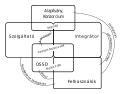
\includegraphics{ábrák/OSSD-szervezeti-környezete.pdf}
\caption{OSSD szervezeti környezete (szerkesztette a
szerző)}\label{fig:OSSDSzerv}
}
\end{figure}

Ezen csoportok együttes hatása alakítja ki a nyílt fejlesztési modell
működési hátterét, jelentősen befolyásolva a végső termék
használhatóságát és biztonsági szintjét. A FLOSS termékből közvetlenül
hasznot húzó szolgáltatók és integrátorok fizetett fejlesztőkön
keresztül igyekeznek biztosítani a projekt számukra kedvező irányát, míg
a felhasználók -- akik sok esetben egyben fejlesztők is -- élvezhetik a
két csoport nyújtotta termékeket és szolgáltatásokat.

A támogatások és irányítás gyakran formális kereteket ölt konzorcium
vagy alapítvány formájában, amelyet minden érdekelt fél támogathat, míg
az alapítvány jogi és társadalmi hátteret biztosíthat a közös
fejlesztésnek.

\hypertarget{fejlesztux151kuxf6zuxf6ssuxe9g-feluxe9puxedtuxe9se}{%
\subsubsection{Fejlesztőközösség
felépítése}\label{fejlesztux151kuxf6zuxf6ssuxe9g-feluxe9puxedtuxe9se}}

Az OSSD közösségek sokkal inkább hasonlítanak egy szociális hálózatra
{[}204{]} vagy a megoszló hálózatokra {[}205{]} mint hagyományos
fejlesztőcsapatra. Bárki részt vehet bennük, bonyolult, határokon
átívelő rendszert alkotnak{[}52, 134{]} és a kapcsolattartás döntő
részben a hálózaton keresztül zajlik. A nagy földrajzi kiterjedés miatt
az időeltolódás problémákat okozhat {[}206{]}.

A közösség rugalmas, könnyen változik, szerkezetét tekintve pedig
általában egy központi mag részből, és az azt körülvevő további külső
rétegekből áll, hagymaszerű struktúrát hozva létre {[}207, 208{]} lásd
fig.~\ref{fig:HagymaModell}. A mag rész tagjai hozzák a legfontosabb
döntéseket, általában csak nekik van joguk módosítani a központi
forrástárakat és jobbára hosszú időn keresztül a projektben
tartózkodnak{[}209{]}. A magot körülvevő fejlesztői holdudvar a magtól
távolodva egyre ritkábban adományoz kódot és egyre kisebb szerepet
vállal a fejlesztésből. A teljes fejlesztőtábor lehet egészen nagy, több
ezer fős, de a közösség méretének növekedésével egyre kisebb a
hozzáadott fejlesztőerő {[}210{]} igazolva, hogy a nyílt modellre is
igaz a Ringelmann hatás.

\textbf{A magfejlesztők} kis csoportja adja a projekt gerincét, az
érdemi munka döntő hányadát is gyakran ők végzik{[}134, 156, 211{]}, sőt
a magfejlesztők nem egyszerűen csak többet dolgoznak, hanem minőségileg
más munkát végeznek{[}212{]} (a hagyma ``magja'' tehát kissé eltérő). A
mag mérete változhat de a legtöbb projektben 15 fő alatt marad
{[}213{]}. A magfejlesztők között lehetnek ``hősök'', pótolhatatlan
személyek ami termelékenységi szempontból hasznos {[}214{]} ám egyben
kockázati tényező is, ugyanis a centrális emberek kiesése komolyan
sértheti a csoport teljesítményét {[}215{]}. Az akadémiai projektként
indult GIMP fejlesztése például több mint egy évre leállt, mert vezető
fejlesztői befejezték az iskolát és elmentek dolgozni. Eddig tartott míg
valaki más felvette a stafétabotot {[}152{]}. Ugyanakkor empirikus
bizonyítékok támasztják alá, hogy a közepesnél nagyobb nyílt projektek
döntő része ``hős-projekt'', ahol a fejlesztés 80\%-át, a fejlesztők
20\%-a végzi {[}216{]}.

\textbf{Az aktív fejlesztők} jó rálátással rendelkeznek a projektre,
idővel beléphetnek a magfejlesztők közé, bevonják őket a kulcsfontosságú
döntésekbe, de szerepük marginális.

\textbf{Az alkalmi fejlesztők} csoportja a legnagyobb, ők egyetlen
funkcióra vagy hibajavításra koncentrálnak. E csoport határán
helyezkednek el az egyszeri fejlesztők akik valamikor hozzájárultak a
projekthez, ám végül különféle okok miatt (időhiány, érdektelenség)
végül eltávolodtak attól{[}217{]}.

A nagyobb projektekben általában cégek is adományoznak kódot, illetve
saját fejlesztőkön keresztül igyekeznek a mag közelébe kerülni
{[}186{]}. Barham szerint a minőségbiztosítással foglalkozó közösségi
tagok -- ha vannak -- külön réteget képeznek a hagyma-modellben és
viszonylag elkülönülő kommunikációt folytatnak {[}218{]}

\begin{figure}
\hypertarget{fig:HagymaModell}{%
\centering
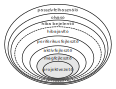
\includegraphics[width=0.5\textwidth,height=\textheight]{ábrák/hagyma-modell.pdf}
\caption{OSSD hagyma modell (saját változat Di Bella nyomán
{[}207{]})}\label{fig:HagymaModell}
}
\end{figure}

Bird szerint a magot körülvevő közösség felépítése sem homogén hanem kis
csoportokra, modulokra bomlik, akik egymással sűrűbben kommunikálnak,
esetleg saját központi tagjaik vannak {[}219{]} vagyis a homogén hagyma
modell kissé megtévesztő. A szponzorált fejlesztők jelenléte tovább
növeli a modularitást, az egy céghez tartozók között szorosabb a
kapcsolat{[}220{]}. Ez a struktúra segít, hogy a fejlesztőszám
növekedésével a kommunikációs overhead ne váljon kezelhetetlenné
{[}221{]}. A decentralizált projektek jellemzően modulárisabbak mint a
centralizáltak, a kisebbek pedig többnyire a hierarchikus típusból
indulva érik el a decentralizált állapotot {[}222{]}. A viszonylag kis
mag kialakulása nem hiányosság, hanem szükségszerű következmény, ugyanis
egy nagyobb létszámú központi csoport tagjaira kezelhetetlenül nagy
kommunikációs teher nehezedne.

Forrest lehetséges problémaként azonosította a hibabejelentők és a
fejlesztők elkülönülését. A két csoport csoporton belül sokat
kommunikál, ám a legjelentősebb fejlesztők a hibabejelentőkkel nem
kommunikálnak {[}223{]}, ami arra enged következtetni, hogy a gyors és
hatékony hibajavítások érdekében a FLOSS felhasználó szervezetnek
csatlakoznia kell a fejlesztéshez.

Bizonyos projektek saját biztonsági csapattal is rendelkeznek (pl.
Drupal) akik a biztonsággal kapcsolatos figyelmeztetéseket figyelik és
értékelik, illetve folyamatosan hibákat keresnek az alkalmazásban
{[}224{]}. Ez a jelenség azonban nem általános és formális követelmények
nélkül hatékonysága is megkérdőjelezhető. Ruohonen et al.~CVE
sérülékenység jelentések analízise segítségével arra a megállapításra
jutott, hogy a sérülékenységek jelentése általában kis számú
magfejlesztőhöz fűződik {[}225{]}.

Az irányított és szponzorált nyílt közösségek szignifikánsan több
fizetett fejlesztőt alkalmaznak és jóval több a módosításra jogosult
fejlesztők száma {[}226{]}. A magot körbevevő holdudvar végzi a
tesztelés, hibakeresés nagy részét, a végső döntést és a kiadási
ütemezést általában az irányító ipari szereplő határozza meg. Az
irányított közösségekben érdemes megkülönböztetni a kettős licencelést
alkalmazó, egyetlen cég köré épült projekteket{[}155{]}, illetve a közös
cél érdekében egyesülő cégcsoport által vezetett projekteket
(technológiai konzorcium). Liu szerint tisztán szervezetekből álló nyílt
közösség is létrejöhet, ezt Community Source-nak nevezte {[}227{]}.

A fejlesztői szervezet tulajdonképpen egy speciális szociális hálózatnak
tekinthető. A szociális hálózatokat fenyegető veszélyforrások itt is
érvényesek lehetnek, annyi különbséggel, hogy a ``felhasználók'' ebben
az esetben technikai téren minden bizonnyal felkészültebbek. A
fenyegetések beazonosítása és mérséklése tekintetében a szociális
hálózatokkal kapcsolatos kutatások lehetnek mértékadóak.

\hypertarget{szociuxe1lis-struktuxfara}{%
\subsubsection{Szociális struktúra}\label{szociuxe1lis-struktuxfara}}

A közösség szociális struktúrája és ideológiai beállítottsága direkt
hatást gyakorol a jelentkezésekre és a döntéshozatalra, így a teljes
projekt teljesítményére {[}228{]}. Alapvetően szociális struktúráról
lévén szó, a társakról alkotott vélemény és kapcsolattartás különösen
fontos OSSD esetén. A felek gyakran csak egymás digitális valóját
ismerik, gyakori a köszönetnyilvánítás, üdvözlés, a pozitív atmoszféra
fenntartása. Az együttműködés alapja első sorban a bizalom és nem a
tekintély. A bizalom elvesztésének fő oka a rossz kód (pl. kritikus
hibák bevezetése, tervezési egység megsértése), kis mértékben szociális
tényezők. A közösségekben régebb óta részt vevő felek sokkal hamarabb
közös nevezőre tudnak jutni {[}229{]}, vagyis a közösségi kommunikáció
tanulható, fejleszthető. A jellegzetes szociális közegnek -- a ``hekker
etikának'' -- úgy tűnik jelentős szerepe van abban, hogy a nyílt
közösség egyedi fejlesztési módszertana jól működik. A tudásmegosztás és
viszonzás kultúrája a kódátnézések során is érvényesül {[}230{]}.

A személyes találkozások hatása egyértelműen pozitív {[}231{]} a
találkozókon való részvétel tehát segít a kapcsolatépítésben, a
prominens fejlesztők jelentős része gyakran személyesen is ismeri
egymást {[}232{]}. Rendszeres személyes kapcsolat híján a
szoftverfejlesztés egyes folyamatai, például a kódellenőrzés segít a
munkatársakról formált kép kialakításában, ugyanakkor -- vagy épp ezért
-- a kódellenőrzés vagy belső kommunikációs során használt udvarias
szociális forma nagyobb jelentőséggel bír {[}133, 233{]}.

\hypertarget{uxe1tluxe1thatuxf3suxe1g}{%
\subsubsection{Átláthatóság}\label{uxe1tluxe1thatuxf3suxe1g}}

Az közösség működése és felépítése szinte minden esetben átlátható. Igaz
ez az információ nem közvetlenül publikált (nincs szervezeti diagram) de
a metainformációk alapján könnyen felmérhető és elemezhető {[}228,
234{]}. Az OSSD projektek nyíltan működnek és minden érdeklődő
közeledését szívesen veszik. Szabadon elérhető a szervezettel
kapcsolatos (bár bizonyos területeken szegényes) minden dokumentáció,
napló, beszélgetés {[}235{]}.

Az átláthatóság segíthet felmérni a nemzetbiztonsági kockázatokat annak
ellenére, hogy a szervezet általában nemzetközi. Egy határon túli vállat
üzletmenetébe meglehetősen problémás belelátni, nehezen átvilágítható a
motivációja és azok a kényszerek amelyeknek -- általában publikálatlanul
-- meg kell felelnie. Elég az elmúlt évek nagyobb adatgyűjtési
botrányaira gondolni a Facebook vagy a Twitter kapcsán. Ráadásul
értelemszerűen felmerül a kérdés, hogy vajon mekkora nyomást tud
gyakorolni egy vállalatra a működési környezetét biztosító nemzetállam.
A klasszikus nyílt közösségekre messzemenően nehezebb nyomást
gyakorolni, pláne elrejteni annak nyomait.

A közösségre élénk kommunikáció jellemző és a kommunikációs adat szinte
minden esetben könnyen hozzáférhető{[}236{]}, igaz az utóbbi években a
kommunikációs csatornák portálokra tolódásával (pl. Slack) ez a nyíltság
-- legalábbis az információ birtoklása és perzisztenciája tekintetében
-- veszélybe kerülhet{[}43, 237{]}. Általában megállapítható az egyes
szereplők munkaköre, szerepe, a munkaerő kihasználásának hatékonysága és
ideje {[}238, 239{]}. A fejlesztő-fejlesztő és fejlesztő-szoftvertermék
közötti interakció analízise révén értékes információ gyűjthető amely
felhasználható a termék minősítése és kockázatbecslés során. Yahav at
al.~javasolják, hogy ez a megfigyelés és elemzés folyamatos legyen, azaz
a közösség állapotát folyamatosan monitorozzuk {[}240, 241{]}, Smith
pedig modell alapú megközelítést tanácsol {[}242{]}.

A fejlesztők beazonosíthatósága komoly előnyt jelenthet komponens
integráció során, hiszen közvetlenül azzal az emberrel lehet felvenni a
kapcsolatot, aki az adott komponenst készítette{[}150{]}. Erre IP,
üzleti titok és szervezési okokból kifolyólag vajmi kevés esély van az
üzleti modell esetén. A vezető fejlesztőket a kommunikációban elfoglalt
centralitásuk alapján lehet beazonosítani {[}243, 244{]}.

A fig.~\ref{fig:figCompDevStruct} ábrán a Mozilla Firefox projekt
fejlesztőinek komponensekhez rendelése látható, míg a
fig.~\ref{fig:figCompDevStruct} ábrán ugyanezen projekt hibajegyekből
generált fejlesztői centralitás vizualizációja figyelhető meg, amelyből
kitűnik, hogy a bzbarsky@mit.edu és a asa@mozilla.org fejlesztők magas
centralitás-értékekkel rendelkeznek (így az ábra közepe táján
találhatóak), valódi nevük és kilétük egyszerű keresőhasználattal
perceken belül kideríthető.

\begin{figure}
\centering

\subfloat[Komponens-fejlesztő
viszony]{\includegraphics[width=0.5\textwidth,height=\textheight]{ábrák/component-developer-relationship_sureka_using_2011.png}\label{fig:figCompDevStruct}}
\subfloat[Mag periféria
minta]{\includegraphics[width=0.5\textwidth,height=\textheight]{ábrák/core-periphery-pattern_sureka_using_2011.png}\label{fig:figPeriphery}}

\caption{Példa a szervezeti felépítés vizualizációjára.
Forrás:{[}244{]}}

\label{fig:OSSD_struct}

\end{figure}

Hasonlóképpen elemezhető a projekt fejlesztő dinamikája is, azaz projekt
fejlesztő-megtartó és fejlesztő-vonzó képessége{[}245{]}, melynek
segítségével akár az egyes fejlesztők kilépésének valószínűsége is
megjósolható {[}215{]}.

\hypertarget{uxf6nszervezux151duxe9s}{%
\subsubsection{Önszerveződés}\label{uxf6nszervezux151duxe9s}}

A közösség egy célkitűzés, ideológia és kulcsemberek köré
szerveződik{[}115{]}. A csoport sikere alapvetően a közösségtől, annak
szerveződő-képességétől függ. Ha a nem sikerül kellő számú hatékony
fejlesztőt vonzania, aligha lehet sikeres {[}246{]}.

A tagok általában maguk választanak maguknak feladatot {[}71, 74, 80{]}
azaz a feladatok kiosztása is önszerveződő. Nem lehet valakit utasítani
vagy elbocsájtani, nincs fejlesztő felvétel és alkalmassági vizsga,
ehelyett fejlesztő-bevonzás van {[}81{]}. A humán erőforrás menedzsment
nem is hasonlít az üzleti világban megszokotthoz {[}74{]}. A kevéssé
népszerű feladatok elvégzése kapcsán a belépő szervezetek szerepe
felértékelődik, hiszen megfelelő (általában anyagi) motivációval
kiegyensúlyozhatja az egyenlőtlenségeket. A munkamegosztás egy
közösségen belül lehet jól definiált, vagy teljesen ad-hoc jellegű is
{[}77{]}.

Gyakran megfigyelhető valamilyen mentori szisztéma, amelynek során egy
régebbi tapasztalt fejlesztő segíti az újonnan beszállni kívánót. A
mentorált csatlakozók mérhetően hatékonyabbak mint az önállóak
{[}247{]}, és a szociális akadályok leküzdésében is sokat segíthet egy
jó mentor, annak híján pedig egy csatlakozni kívánóknak szóló dedikált
honlap{[}248, 249{]}.

Az önszerveződés nem jelenti azt, hogy nincs szükség menedzsmentre. A
fejlesztői hálózat szervezését elhanyagoló projektek sokkal rosszabbul
teljesítenek, gyakran meg is szűnnek {[}164{]}. A kisebb, önjelölt
vezérrel rendelkező projektek legfeljebb akkor tudnak fejlődni, ha
valamilyen módon fel tudják kelteni a figyelmet {[}108{]}. A nagyra
növő, rosszul szervezett projektekben pedig a nehézkes kommunikáció
megnöveli a feladatok lezárásához szükséges időt {[}250{]}.

Érdekes megfigyelés, hogy a résztvevők döntő többsége csak kevés
(gyakran egyetlen) projektben vesz részt, és csak nagyon kevesen ismerik
az egész projektet {[}251, 252{]}. Ez arra enged következtetni, hogy a
jó fejlesztőkért komoly a verseny, a nyílt közösségben szerepet vállalni
kívánók száma{[}239{]} és a fejlesztésre szánható idő is véges.
Következésképpen a nyílt közösség megtartása és vonzása érdekében
érdemes bizonyos marketing tevékenységet végezni.

\hypertarget{duxf6ntuxe9shozatal-iruxe1nyuxedtuxe1s-befolyuxe1s}{%
\subsubsection{Döntéshozatal, irányítás,
befolyás}\label{duxf6ntuxe9shozatal-iruxe1nyuxedtuxe1s-befolyuxe1s}}

A klasszikus modellben általában nincs világos vezetői lánc, a döntések
sok vitával járnak ami megnöveli a koordinációs erőfeszítéseket
{[}253{]}, a nagyobb projektek (talán épp emiatt) centralizáltabb
döntéshozatalt alkalmaznak, ugyanakkor a döntések és indoklások szinte
mindig átláthatóak maradnak (lásd még: \ref{sec:FS-K-Sz}), máskülönben
elidegenítik a fejlesztőket és leépítik a közösséget. Nincs alkalmazható
kényszer, így bizonyos népszerűtlen feladatok elvégzetlenül maradnak,
illetve a nagyobb, szponzorált projektekben az ilyen feladatokat
fizetett fejlesztők végzik el{[}105{]}. Gyakori, hogy saját
normarendszert fejlesztenek ami a fejlesztés irányát és a követendő
ideológiát is kijelölti {[}206{]}.

A közösség irányítása lehet decentralizált ``Bazár'' stílusú vagy
centralizált, esetleg hierarchikus felépítésű. A előbbiek általában a
független nem rutinszerű nagy bizonytalanságú feladatokban teljesítenek
jól, míg a rutinszerű, erősen összefüggő, kis bizonytalanságú
feladatokhoz a centralizált felépítés a megfelelőbb {[}254{]}. Az
irányítás jellege lehet oltalmazó, erős irányítás alatt tartva a külső
hozzájárulásokat, technikai jellegű, amely kizárólag a technikai
előnyöket nézi valamint rugalmas, amely a közösség növekedését tartja
szem előtt {[}255{]}.

A vezetők -- klasszikus esetben -- kis részben hagyomány, nagyobb
részben alkalmasságuk alapján kerülnek kiválasztásra többnyire
demokratikus formában, így a klasszikus nyílt közösség meritokráciának
vagy technokráciának tekinthető{[}115{]}. A bizalom kiépítésénél a
legfontosabb tényezők a fejlesztői tudás, a reputáció valamint a
formális és informális tevékenység a közösségen belül {[}125, 256{]}. A
vezetők szerepe és kiléte meghatározó {[}220{]}, egy-egy vezéralak
véleménye nagy súllyal eshet latba a döntéseknél. A gitHubon belül
például a GitHub csapat tagjai, a szervezetek, az OSSD fejlesztők és a
keretrendszer/progamkönyvtár szerzők rendelkeztek a legmagasabb bizalmi
szinttel {[}257{]}. A hatásgyakorlás inkább csak belülről lehetséges,
ezért a szoftvercégek gyakran szponzorálnak fejlesztőket akik képviselik
az érdekeiket {[}258, 259{]}. Aaltonen az e-mail címek elemzése alapján
kimutatta, hogy az iparági szereplők befolyása meglehetősen nagy,
például a Linux kernel projektben {[}134{]} (jellemző szereplők: Redhat,
HP, Oracle, Intel, IBM) vagy Debian operációs rendszerben {[}260{]}
(SUN, Xerox, Digital Equipment corp, Silicon Graphics, HP stb.). A Linux
kernel esetében mára a vállalati hozzájárulás mértéke meghaladja a
független hozzájárulások mértékét {[}261{]}. A nyílt projektben való
részvétel egyik kockázata az irányítás elvesztése {[}262{]}, az új
közösség kiépítése pedig igen költséges és időigényes.

A közösség fontos döntéseiben a mag csoport tagjainak sokkal nagyobb
szerepe van, az egyéb módon fel nem oldható vitás kérdéseket is ők
rendezik {[}263{]}. Emiatt fontos e szereplők beazonosítása, hiszen
segítségükkel lehet leginkább hatni a csoportra, illetve ezeket a
szereplőket érdemes a szervezetnek támogatni. {[}207{]}. A döntéshozatal
általában nem teljesen demokratikus, a mag résztől távolabb esőknek
kevesebb beleszólásuk van a döntésekbe, illetve a mag élén állók gyakran
fenntartják maguknak a jogot a végső döntésre. A vezérek sem tehetnek
meg bármit, hiszen ha szembe mennek a közösséggel akkor annak
elvesztését vagy a projekt másolását (fork) kockáztatnák. Legtöbb
projekt esetében tehát a végső döntés közösségi nyomásra jön létre,
nagyon sokat számít, hogy a változtatni kívánó fél mekkora lobbierőt tud
felvonultatni, hány embert tud maga mellé állítani {[}101{]}. A
változásokat egyáltalán nem olyan egyszerű keresztülvinni, mint az ember
elsőre gondolná. Ennek oka, hogy a szoftver óriásira duzzadna ha bárki
beletehetné kedvenc funkcióját (feature bloat), ami ellen a fejlesztői
közösség általában keményen fellép {[}105{]}.

Az OSSD menedzsment vonatkozásai merőben eltérnek az üzleti
fejlesztéstől. Vannak megrögzötten független fejlesztők, akik igen
nehezen viselik ha a projekt mögött egy nagyobb cég áll {[}204{]}.
Emiatt fontos lehet a szervezet (érzékelhető) jelenlétét a lehető
legkisebbre csökkenteni. Az ipari szereplőknek viszont könnyen megérheti
a közösséghez való csatlakozás, vagy saját közösség létrehozása, hiszen
a közösség által, fejlesztőkhöz, informális tesztelőkhöz és rengeteg
visszajelzéshez jutnak {[}185, 264{]} valamint növelhetik befolyásukat a
projekt céljait illetően{[}258{]}. Bármilyen nagy is egy cég, annyi
fejlesztőt egyszerűen nem bír megfizetni, amennyi egy komolyabb OSSD
projektben összegyűlik{[}75, 265{]}. Következésképpen a szervezet
felépítése gyakorta bővül fizetett fejlesztőkkel és iparági
kapcsolatokkal.

A klasszikus OSSD nyitottsága természetszerűleg támogatja a
belépést{[}266{]}, a meritokrácia jelleg miatt a cégeknek gyakran nincs
is más lehetőségük az irányításra. A belépés -- mint láttuk -- általában
meg is éri, ugyanakkor adaptálódni kell az adott projekt
kultúrájához{[}267{]} nagyon nehéz megváltoztatni azt. Nem előnyös
például ha a saját fejlesztők külön csatornán kommunikálnak. A közösség
átláthatóságot vár{[}64{]}. Nem javasolt továbbá a modern extreme
programozási\footnote{Extreme Programming. Modern szoftverfejlesztés
  módszertan az agile software development egyik ága. Jellegzetes
  technikái a páros programozás, extenzív kódvizsgálat, hierarchia
  nélküli menedzsment és a gyakori interakció az ügyféllel.} technikák
használata sem, amelyek zárttá teszik a csoportot {[}268{]}.

Ha a cég jelenléte nagy, akvizíciója komoly veszélyt jelenthet a projekt
jövőjére nézve és súlyos zavart kelthet a közösségen belül még akkor is,
ha a terméket érintően semmilyen változtatás nem történik {[}269{]}.
Hasonlóan súlyos lehet a helyzet ha a cég elhagyja a korábban vezetett
projektet akkor is, ha korábban az nélküle működőképes volt {[}36{]}.

Amennyiben egy gazdasági szereplő hatást szeretne gyakorolni a
közösségre, a következő lehetőségei vannak{[}270{]}:

\begin{itemize}
\tightlist
\item
  integráció: a szervezet beépül a közösségbe. Szerepe nem
  szükségszerűen vezető, a közösség által előállított FLOSS
  komponensekből származó haszon az együttműködés célja.
\item
  közösség létrehozása: a szervezet maga hozza létre a közösséget. A
  kulcskérdés itt a közösség szervezése, de az integrációval ellentétben
  a szervezet saját üzleti stratégiájához illeszkedő erőforrásként
  kezeli a közösséget.
\item
  hatalomátvétel: a szervezet egy létező OSSD közösség felett veszi át
  az irányítást céljait tekintve a létrehozással azonos.
\item
  másolás (fork): a szervezet saját független változatot indít a FLOSS
  termékből. Ez általában akkor következik be ha az integrációt követően
  a közösség olyan irányt vesz fel amely a szervezet üzleti vagy
  stratégiai céljaival összeegyeztethetetlen. A forkolt közösség feletti
  irányítás átvétele lehetséges, de nem követelmény, hiszen a forkolt
  változatot követő fejlesztők oszthatják a szervezet nézeteit.
\item
  kiadás: a szervezet nyílt forrásúként ad ki egy terméket, de nem
  foglalkozik vele, hogy épül-e köré közösség vagy sem. Ez a stratégia
  figyelhető meg többek között a kormányzati szektorban, ahol a
  kormányzati forrásokból készült terméket OSI kompatibilis licenccel
  adják ki.
\end{itemize}

A kód megnyitása vagy új közösség szervezése korántsem jelent garantált
sikert. Könnyen előfordulhat, hogy a közösség nem nő, az újonnan érkezők
egyetlen alkalom után továbbállnak, elvesztik érdeklődésüket vagy
forkolják a projektet{[}271{]}.

Schaarschmidt szerint az üzleti szereplők alapvetően kétféleképpen
fejthetnek ki hatást a nyílt közösségekre{[}226{]}:

\begin{itemize}
\tightlist
\item
  \emph{irányítás a vezetésen keresztül}: saját embereiket juttatják a
  közösség vezető pozícióiba vagy megfizetik az eleve ott található
  fejlesztőket;
\item
  \emph{irányítás erőforrás-bevitel segítségével}: vállalati
  környezetben szocializálódott fejlesztőket juttatnak a közösségbe, és
  klánkontroll segítségéve formálják annak szokásait. A későn belépő
  szervezet számára gyakran csak ez a lehetőség nyitott, mert csak
  nehezen tud vezető pozíciókat megszerezni.
\end{itemize}

A fizetett fejlesztők valószínűleg ténylegesen nagyobb hatást képesek
kifejteni a közösségre, mindenesetre több emberrel kommunikálnak, velük
is több ember keresi az interakciót{[}258{]} és a centralitási értékeik
is magasabbak {[}250{]}. Nem csak a cég számára előnyös a közösség, ez
fordítva is igaz, a közösség helyezését is emeli a cégek
belépése{[}63{]}. Emiatt hasznos lehet a fizetett fejlesztők
(automatizált) beazonosítása {[}272{]}. A kisebb, kiforratlanabb
közösségek esetében általában komolyabb erőforrás befektetéssel lehet
elérni a szervezet által kívánatos célok teljesülését, a megállapodott
projektek esetében viszont a belépés lényegében csak a hibajegyek
felvételére korlátozódik, a kitűzött irányon nagyon nehéz változtatni
{[}273{]}.

A nagy OSSD projektek irányítása sok tekintetben hasonlít a politikára,
egzakt módon nehezen megfogható szociális vonatkozásai vannak {[}274{]},
sok szereplő küzd különféle módszerekkel a befolyásért {[}101, 235{]} és
néha ütköznek az érdekek. A projekten olyan vállalatok dolgozhatnak
együtt, akik nyílt piaci környezeteben vetélytársak. Teixeira például
megfigyelte, hogy a vállalatok gyakran beviszik saját ellentéteiket a
közösségbe {[}275{]} ami a nyílt projekt mérhető sérüléséhez vezet. A
vállalatok dedikált technikákat alkalmaznak, hogy belső, minősített
információk ne szivároghassanak ki a nyílt együttműködésen keresztül
{[}276{]}: a megosztott adatokat üzleti szempontok szerint szűrik és
felelősöket ``Gatekeeper''-eket jelölnek ki, akik a szervezet határán
állva ellenőrzik az információ-áramlást.

Amennyiben a szervezet stratégiai fontosságú nyílt forrású komponenseket
hasznosít, a projekttel való valamilyen szintű együttműködés
mindenképpen javasolt, adott esetben szinte elkerülhetetlen. A részvétel
történhet közvetlenül szervezeti keretek közt, állami szinten vagy
alapítványok formájában {[}277{]}.

\hypertarget{sec:FS-K-R}{%
\subsection{Résztvevők (FS-K-R)}\label{sec:FS-K-R}}

Mint kiderült a kulcsszereplők beazonosítása igen fontos, ez azonban
nehézségekbe ütközhet. Nem csak a konkrét személy identitását lehet
nehéz megállapítani, hanem az egyes pszeudo-anonim identitások (e-mail,
nick, álnév, cím stb.) azonosságát is{[}278{]}. Néha a személyazonosság
pár perces kereséssel kideríthető, más esetben -- különösen ha a
fejlesztő szándékosan rejtőzködik -- a feladat közel lehetetlen. Jó
példa erre Satoshi Nakamoto, a Bitcoin hálózat tervezője, akinek kilétét
az amúgy jelentős erőfeszítések ellenére is mind a mai napig homály
fedi. Még azt sem sikerült hitelt érdemlően megállapítani, hogy egyetlen
személyről vagy egy csoportról van-e szó. Ugyanakkor az egyes fejlesztők
kódolási stílusa imitálható, így egy esetleges támadó megkísérelheti
megtéveszteni a közösséget {[}279{]}. Ennek elkerülésére ugyan már
léteznek javaslatok, de a gyakorlatban jelenleg még nem alkalmazzák
őket.

Nem triviális összevetni, hogy egy adott módosítást végző személy
azonos-e egy másik módosítást végző személlyel, a program vezető
fejlesztőjével vagy a hibajegyet kezelő személlyel. Ezen a problémán
segíthet valamelyest a terjesztett csomaghoz csatolt vagy verziókezelő
rendszerben, disztribúció csomagjaiban tárolt digitális aláírás. Sajnos
sok esetben a fejlesztők több ilyen aláírást is használnak (elvesztés,
frissítés) tehát a módszer korántsem száz százalékos és gyakran csak a
pszeudo-identitáshoz rendelés lehetséges.

A résztvevők sokféle környezetből érkeznek, vannak közöttük kiváló
szakemberek{[}105{]}, hátterük igen eltérő mind életkorra, származásra
és képzettségre való tekintettel {[}280{]}. Általában jó csapatjátékosok
és alapvetően implementáció orientáltak {[}65{]}.

Az üzleti fejlesztés profitvezérelt (külső motiváción alapul), a nyílt
fejlesztést (elsősorban belső) motivációk hatásegyüttese jellemzi.
Fejleszthet valaki azért mert tanulni akar, vagy hiányzik egy rég kívánt
képesség a kedvenc szoftveréből, vagy egyszerűen az alkotás öröméért,
vagy a társadalom iránti elkötelezettségből, altruizmusból{[}80{]}. A
következő fő indítékcsoportok motiválhatják a fejlesztőket {[}54,
281--286{]}:

\begin{enumerate}
\def\labelenumi{\arabic{enumi}.}
\tightlist
\item
  Altruizmus (személyes hit a OSSD-ben, nyomot hagyni a világban,
  segíteni másokon)
\item
  Külső motiváció (karrier lehetőségek, előmenetel, szociális státusz,
  díjak)
\item
  Tudásbővítés (területi érdeklődés, új helyek, emberek, eszközök
  megismerése);
\item
  Közösségi,szociális indokok (csoporthoz tartozás, kommunikáció,
  tudásmegosztás)
\item
  Belső késztetés (munka öröme, önkifejezés, szórakozás, irányítás
  érzése)
\item
  Személyes igények kielégítése (hiányzó funkciók elkészítése);
\end{enumerate}

A korábban belső indokok miatt fejlesztők motivációja nem változik meg
akkor sem ha munkájukért fizetést kapnak {[}283{]}.

A fizetett fejlesztők motivációja külső, fajtái az alábbiak
lehetnek{[}287{]}:

\begin{itemize}
\tightlist
\item
  szabad szponzorálás, Nincs konkrét instrukció az alkalmazótól;
\item
  alkalmazotti viszony, világos feladatokkal;
\item
  részlegesen kötött, a fejlesztő ideje egy részével rendelkezhet;
\item
  adott cél eléréséért kapott díj, megbízási viszony.
\end{itemize}

A belső motivációból előnye, hogy erősebb mint a külső motiváció
{[}205{]} hátránya viszont az irányíthatóság hiánya, így például a belső
indíttatásból fejlesztők nem igazán kedvelik az adminisztrációt
{[}288{]}, az ``unalmas'' feladatokat {[}76{]}, kedvelik viszont a
nyíltságot, kényesek a kommunikáció minőségére, a termék nyíltságára
{[}289{]} valamint a licencre {[}290{]}, könnyen előfordulhat, hogy
kifejezetten elutasítóak a zárt forrású rendszerekkel szemben {[}291{]}.

A motiváció ismerete fontos, ugyanis ha a szervezet befolyást akar
gyakorolni a közösségre saját delegált emberei által, a delegáltaknak
tisztában kell lenniük a OSSD fejlesztők motivációival, ha tudni akarják
hogyan hathatnak rájuk{[}292{]}. Az egyik érdekes lehetőség a
gamifikáció, vagyis a repetitív, népszerűtlen feladatok játékos formába
öntése {[}293{]}.

\begin{longtable}[]{@{}rcll@{}}
\caption{A \emph{K} kategóriában azonosított problémák}\tabularnewline
\toprule
\begin{minipage}[b]{0.03\columnwidth}\raggedleft
kód\strut
\end{minipage} & \begin{minipage}[b]{0.03\columnwidth}\centering
szint\strut
\end{minipage} & \begin{minipage}[b]{0.69\columnwidth}\raggedright
leírás\strut
\end{minipage} & \begin{minipage}[b]{0.13\columnwidth}\raggedright
sajátosság\strut
\end{minipage}\tabularnewline
\midrule
\endfirsthead
\toprule
\begin{minipage}[b]{0.03\columnwidth}\raggedleft
kód\strut
\end{minipage} & \begin{minipage}[b]{0.03\columnwidth}\centering
szint\strut
\end{minipage} & \begin{minipage}[b]{0.69\columnwidth}\raggedright
leírás\strut
\end{minipage} & \begin{minipage}[b]{0.13\columnwidth}\raggedright
sajátosság\strut
\end{minipage}\tabularnewline
\midrule
\endhead
\begin{minipage}[t]{0.03\columnwidth}\raggedleft
SK01\strut
\end{minipage} & \begin{minipage}[t]{0.03\columnwidth}\centering
1\strut
\end{minipage} & \begin{minipage}[t]{0.69\columnwidth}\raggedright
A fejlesztők és a hibabejelentők közötti kommunikáció nem
megfelelő.\strut
\end{minipage} & \begin{minipage}[t]{0.13\columnwidth}\raggedright
FS-K-Sz\strut
\end{minipage}\tabularnewline
\begin{minipage}[t]{0.03\columnwidth}\raggedleft
SK02\strut
\end{minipage} & \begin{minipage}[t]{0.03\columnwidth}\centering
1\strut
\end{minipage} & \begin{minipage}[t]{0.69\columnwidth}\raggedright
Az alkotók nem mindig beazonosíthatók. Nehéz megállapítani, hogy több
részmunkát ugyanaz a személy végezte-e el vagy sem.\strut
\end{minipage} & \begin{minipage}[t]{0.13\columnwidth}\raggedright
FS-K-Sz\strut
\end{minipage}\tabularnewline
\begin{minipage}[t]{0.03\columnwidth}\raggedleft
SK03\strut
\end{minipage} & \begin{minipage}[t]{0.03\columnwidth}\centering
1\strut
\end{minipage} & \begin{minipage}[t]{0.69\columnwidth}\raggedright
Az erős cégirányítás miatt a fejlesztők elhagyják a projektet,
veszélyeztetve a támogatást\strut
\end{minipage} & \begin{minipage}[t]{0.13\columnwidth}\raggedright
FS-K-Sz\strut
\end{minipage}\tabularnewline
\begin{minipage}[t]{0.03\columnwidth}\raggedleft
SK04\strut
\end{minipage} & \begin{minipage}[t]{0.03\columnwidth}\centering
4\strut
\end{minipage} & \begin{minipage}[t]{0.69\columnwidth}\raggedright
Rossz vagy az elvárásoknak nem megfelelő kód küldése a bizalom, ezáltal
az OSSD feletti irányítás elvesztését okozza.\strut
\end{minipage} & \begin{minipage}[t]{0.13\columnwidth}\raggedright
FS-K-Sz\strut
\end{minipage}\tabularnewline
\begin{minipage}[t]{0.03\columnwidth}\raggedleft
SK05\strut
\end{minipage} & \begin{minipage}[t]{0.03\columnwidth}\centering
1\strut
\end{minipage} & \begin{minipage}[t]{0.69\columnwidth}\raggedright
Az OSSD vezető szereplője távozik (cég akvizíciója, fejlesztő kilépése),
a támogatás folytonossága veszélybe kerül.\strut
\end{minipage} & \begin{minipage}[t]{0.13\columnwidth}\raggedright
FS-K-Sz\strut
\end{minipage}\tabularnewline
\begin{minipage}[t]{0.03\columnwidth}\raggedleft
SK06\strut
\end{minipage} & \begin{minipage}[t]{0.03\columnwidth}\centering
4\strut
\end{minipage} & \begin{minipage}[t]{0.69\columnwidth}\raggedright
A delegált fejlesztők nyílt kommunikációja érzékeny adatokat tesz
publikussá.\strut
\end{minipage} & \begin{minipage}[t]{0.13\columnwidth}\raggedright
FS-K-Sz\strut
\end{minipage}\tabularnewline
\bottomrule
\end{longtable}

\begin{longtable}[]{@{}rcll@{}}
\caption{A \emph{K} kategóriában azonosított javaslatok}\tabularnewline
\toprule
\begin{minipage}[b]{0.03\columnwidth}\raggedleft
kód\strut
\end{minipage} & \begin{minipage}[b]{0.03\columnwidth}\centering
szint\strut
\end{minipage} & \begin{minipage}[b]{0.69\columnwidth}\raggedright
leírás\strut
\end{minipage} & \begin{minipage}[b]{0.13\columnwidth}\raggedright
probléma\strut
\end{minipage}\tabularnewline
\midrule
\endfirsthead
\toprule
\begin{minipage}[b]{0.03\columnwidth}\raggedleft
kód\strut
\end{minipage} & \begin{minipage}[b]{0.03\columnwidth}\centering
szint\strut
\end{minipage} & \begin{minipage}[b]{0.69\columnwidth}\raggedright
leírás\strut
\end{minipage} & \begin{minipage}[b]{0.13\columnwidth}\raggedright
probléma\strut
\end{minipage}\tabularnewline
\midrule
\endhead
\begin{minipage}[t]{0.03\columnwidth}\raggedleft
JK01\strut
\end{minipage} & \begin{minipage}[t]{0.03\columnwidth}\centering
4\strut
\end{minipage} & \begin{minipage}[t]{0.69\columnwidth}\raggedright
A közösségbe fejlesztőket kell delegálni akiknek lehetőség szerint
mentort kell keresni.\strut
\end{minipage} & \begin{minipage}[t]{0.13\columnwidth}\raggedright
SJ01\strut
\end{minipage}\tabularnewline
\begin{minipage}[t]{0.03\columnwidth}\raggedleft
JK02\strut
\end{minipage} & \begin{minipage}[t]{0.03\columnwidth}\centering
2\strut
\end{minipage} & \begin{minipage}[t]{0.69\columnwidth}\raggedright
A belső szerkezet elemezhető, meghatározhatók a kulcsszereplők. Az
adatok alapján kockázatelemzés végezhető.\strut
\end{minipage} & \begin{minipage}[t]{0.13\columnwidth}\raggedright
SF07, ST02\strut
\end{minipage}\tabularnewline
\begin{minipage}[t]{0.03\columnwidth}\raggedleft
JK03\strut
\end{minipage} & \begin{minipage}[t]{0.03\columnwidth}\centering
2\strut
\end{minipage} & \begin{minipage}[t]{0.69\columnwidth}\raggedright
A digitális aláírásokat használó fejlesztők nyílt kulcsait (rendszerint
GPG) be kell szerezni, biztonságos adatbázisban kell tárolni,
hozzáférhetővé tenni és szükség esetén ellenőrizni.\strut
\end{minipage} & \begin{minipage}[t]{0.13\columnwidth}\raggedright
\strut
\end{minipage}\tabularnewline
\begin{minipage}[t]{0.03\columnwidth}\raggedleft
JK04\strut
\end{minipage} & \begin{minipage}[t]{0.03\columnwidth}\centering
2\strut
\end{minipage} & \begin{minipage}[t]{0.69\columnwidth}\raggedright
Folyamatosan monitorozni kell a közösséget.\strut
\end{minipage} & \begin{minipage}[t]{0.13\columnwidth}\raggedright
SK05\strut
\end{minipage}\tabularnewline
\begin{minipage}[t]{0.03\columnwidth}\raggedleft
JK05\strut
\end{minipage} & \begin{minipage}[t]{0.03\columnwidth}\centering
2\strut
\end{minipage} & \begin{minipage}[t]{0.69\columnwidth}\raggedright
Megfelelő lobbierőt kell kiépíteni az érdekérvényesítő képesség
érdekében.\strut
\end{minipage} & \begin{minipage}[t]{0.13\columnwidth}\raggedright
SF07, SH07, ST02\strut
\end{minipage}\tabularnewline
\begin{minipage}[t]{0.03\columnwidth}\raggedleft
JK06\strut
\end{minipage} & \begin{minipage}[t]{0.03\columnwidth}\centering
2\strut
\end{minipage} & \begin{minipage}[t]{0.69\columnwidth}\raggedright
Kapcsolatépítéssel és személyes találkozásokkal erősíthető a közösséggel
való együttműködés (pl.találkozók szervezése).\strut
\end{minipage} & \begin{minipage}[t]{0.13\columnwidth}\raggedright
SF07, SH07, ST02\strut
\end{minipage}\tabularnewline
\begin{minipage}[t]{0.03\columnwidth}\raggedleft
JK07\strut
\end{minipage} & \begin{minipage}[t]{0.03\columnwidth}\centering
2\strut
\end{minipage} & \begin{minipage}[t]{0.69\columnwidth}\raggedright
A vezetőkben tudatosítani kell, hogy az OSSD fejlesztőit más módon kell
motiválni.\strut
\end{minipage} & \begin{minipage}[t]{0.13\columnwidth}\raggedright
SK03, SK04, ST02, ST03\strut
\end{minipage}\tabularnewline
\begin{minipage}[t]{0.03\columnwidth}\raggedleft
JK08\strut
\end{minipage} & \begin{minipage}[t]{0.03\columnwidth}\centering
4\strut
\end{minipage} & \begin{minipage}[t]{0.69\columnwidth}\raggedright
Felelőst kell kijelölni (Gatekeeper) aki a közösséggel való
kapcsolattartást és az oda áramló információt ellenőrzi.\strut
\end{minipage} & \begin{minipage}[t]{0.13\columnwidth}\raggedright
SF07, SF14, SK06, SM05\strut
\end{minipage}\tabularnewline
\begin{minipage}[t]{0.03\columnwidth}\raggedleft
JK09\strut
\end{minipage} & \begin{minipage}[t]{0.03\columnwidth}\centering
4\strut
\end{minipage} & \begin{minipage}[t]{0.69\columnwidth}\raggedright
A közösségbe delegált fejlesztők elkülönített kommunikációja előnytelen,
a közösségi csatornán folyó kommunikáció információtartalmára oda kell
figyelni.\strut
\end{minipage} & \begin{minipage}[t]{0.13\columnwidth}\raggedright
SK06\strut
\end{minipage}\tabularnewline
\bottomrule
\end{longtable}

\hypertarget{metaadatok-fs-m}{%
\section{Metaadatok (FS-M)}\label{metaadatok-fs-m}}

A nyílt és zárt fejlesztések egyik nyilvánvaló különbsége a
rendelkezésre álló nagy mennyiségű fejlesztési információ. Elérhető
például a belső dokumentáció, a forráskód, a viták archívuma és minden
hibajegy illetve azok javítási folyamata. Ezeknek a metaadatoknak a
léte, létrehozása, kezelése és vizsgálata hatással lehet az alkalmazó
vagy integrátor rendszerének biztonsági szintjére is.

A nyílt fejlesztések során a közösség tagjai között zajló
információcsere négy jellemző információs térben valósul meg:

\begin{itemize}
\tightlist
\item
  egyeztetési tér, amely magába foglalja a levelező listákat,
  webportálokat, fórumokat, leveleket és blogokat;
\item
  dokumentációs tér, amely magába foglalja a dokumentációt, a webes
  forrásokat és verzió kezelő rendszerek metaadatait;
\item
  karbantartói tér, amely a hibajegy kezelő rendszerekben tárolt
  információt jelenti;
\item
  és implementációs tér, azaz maga a forráskód az itt található
  megjegyzésekkel együtt.
\end{itemize}

Viorres, Mistrik és Tuunanen {[}294--296{]} a karbantartói teret a
dokumentációs tér alá sorolják, véleményem szerint azonban a hibajegy
követés során alapvetően más jellegű kommunikáció (felhasználó -
fejlesztő) zajlik, más célokkal és hangsúllyal, egyfajta átmenetet
képezve a dokumentációs és implementációs tér között.

\hypertarget{sec:FS-M-H}{%
\subsection{Karbantartói tér, hibajegyek, hibakommunikáció
(FS-M-H)}\label{sec:FS-M-H}}

A nyílt forrású projektek jellemzően használnak valamilyen hibakövető
(bugtracker) rendszert. A nagy projektek esetében ez arány 96\%{[}156{]}
míg a közepes és kisebb projektek esetében valamivel kevesebb. Akárcsak
a projekt többi része ez is nyílt, az itt tárolt adatok és kommunikáció
könnyen hozzáférhető és automatizált módszerekkel elemezhető {[}297{]}.

Számos szabad hibakövető rendszer áll rendelkezésre (Mantis, Redmine,
BugZilla stb.) illetve a népszerű közösségi fejlesztőplatformok (GitHub,
GitBucket) beépítetten is biztosítanak ilyen lehetőséget. Persze a
hibakövető rendszer használata önmagában nem egyedi sajátosság, hiszen a
zárt fejlesztések, sőt szolgáltatók is alkalmaznak valamilyen vagy éppen
valamelyik fent felsorolt hibakövető rendszert. A FLOSS-ra jellemző
egyedi jelenség viszont, hogy ezeket a rendszereket bárki -- komolyabb
authentikáció nélkül -- használhatja{[}298{]}. A használat módja, a
felvitt hibajegyek és azok hasznosulása, kivált pedig a teljes
információmennyiség folyamatos átláthatóság az, ami megkülönbözteti a
nyílt közösséget {[}75, 167{]}.

A szabadon elérhető hibajegy információ automatizált módszerekkel
elemezhető{[}246, 299, 300{]}, adatbányászati technikákkal, kulcsszó
alapú kereséssel értékes információkat kaphatunk a projekt állapotáról,
hibajavító képességéről, szociális szerkezetéről {[}301{]}. A
hibajegy-kezelőből kigyűjtött információkat összevethetjük sérülékenység
adatbázisok adataival {[}302{]}, illetve alkalmazhatunk egyedi modell
alapú hiba-előrejelző rendszert {[}303, 304{]} vagy hagyományos szoftver
megbízhatósági modelleket {[}305{]}. A publikus hibajegyek negatív
hatása, hogy a sérülékenység mindenki számára azonnal elérhetővé válik,
így a sérülékenységet elvben kihasználni képes potenciális támadók köre
is szélesebb.

A hibejegyekhez kapcsolódó de azokkal ellentétben többnyire közvetlenül
a verziókövető rendszerben tárolt commit üzenetek elemzése hasonló
eredményeket hozhat. A mesterséges intelligencia kutatás fejlődésének
köszönhetően például 80\% pontossággal meghatározhatók a biztonsági
problémákhoz kapcsolódó commit üzenetek {[}306{]} így lényegében az
elvégzett javítás és a sérülékenység jellege is beazonosítható. Érdemes
figyelembe venni, hogy ezek a lehetőségek egy esetleges támadó számára
éppúgy elérhetőek. A biztonsági hiba javítását követően eltelik bizonyos
idő (napok, hetek vagy akár hónapok), míg a disztribúciós csatornákon
keresztül a végfelhasználóhoz is eljut a javítás. Ezt az időablakot
kihasználva a támadó előnybe kerülhet.

Az hibajegyekből és commit üzenetekből néhány általános, a nyílt
fejlesztésre jellemző biztonsággal kapcsolatos paramétert is
megtudhatunk. Az alábbiakban ilyen adatokat mutatok be röviden kifejtve
annak esetleges biztonsági hatásait.

A hibajegyeket általában (67\%) konzisztensen kezelik de a megoldatlan
hibák száma 20\% körüli{[}156{]}. A minket érintő hibák tehát nem
feltétlenül lesznek kijavítva, így fontos a részvétel vagy a megfelelő
irányítási és/vagy motivációs lehetőség kiépítése. A sérülékenység száma
az idő előrehaladtával általában növekszik (Apache, Mozilla, Linux)
{[}307--309{]}, ami első hallásra nem vet túl jó fényt a nyílt
fejlesztésekre, bár lehetséges, hogy a hibaszám növekedése nem a minőség
romlását jelzi, egyszerűen csak arról van szó, hogy a felhasználók és a
fejlesztők egyaránt egyre biztonság-tudatosabbá válnak és jobban
odafigyelnek {[}309{]}. A biztonsági bejelentéseket általában más
elbírálásban részesítik és gyorsabban javítják őket {[}310{]}.

A felhasználói interfésszel kapcsolatos visszajelzések általában hamar
megérkeznek{[}311{]}, ami várható is hiszen ezzel a résszel találkoznak
leghamarabb a felhasználók. Bizonyos hibák felderítése és különösen
reprodukálása ugyanakkor igen nehéz lehet (pl. concurrency, race
condition) {[}307, 309{]} ha pedig a reprodukálás valószínűsége
alacsony, a fejlesztők elutasíthatják őket. Nagy figyelmet kell
fordítani tehát a pontos és minél jobb hibakeresési lehetőséget nyújtó
hibajegyek létrehozására, ami különösen nehéz, ha a kiadható gépi
információk halmaza nem tisztázott.

Mivel a nyílt közösségekben nem lehet ``kérni a panaszkönyvet'',
kötelezettség szegési eljárást indítani, de általában reklamálni sem
nagyon érdemes, potenciálisan fontos lehet, hogy megtaláljuk azokat a
módszereket és személyeket akik meg tudják oldani a problémáinkat. Minél
magasabb kapcsolati szinten (lásd. \ref{sec:FS-K-Sz}) áll egy fejlesztő
annál hamarabb javítja a hibákat, viszont minél többet kommunikál, annál
lassabban {[}312{]}.

A hibabejelentések jelentős része egyszerű segítségkérés, valódi értéke
nincs így zajnak tekinthető {[}313{]}. Az értékes hibajegyeket egy szűk
felhasználó kör veszi fel, tehát nem csak viszonylag jól definiált
fejlesztői és hibajavító csoport, de jól elkülönülő hibakereső halmaz is
létezik. Felmerül a kérdés, hogy ezek után a nyílt forrásnál gyakran
felhozott ``many eyes'' elv -- azaz, hogy kellően sok szem minden hibát
észrevesz{[}80{]} -- mennyiben különbözik egy nagyobb vállalat széles
körű béta tesztjétől. Az adatok tanúsága szerint (legalábbis az elemzett
Mozilla szoftver esetében) úgy néz ki nem sokban {[}300{]}. A
forráskódot nem feltétlenül nézik át ténylegesen és amennyiben átnézik
nem feltétlenül fedik fel a biztonsági sérülékenységeket {[}314{]}.
(Amint azt a fejlesztésről szóló \ref{sec:FS-F-P} szakaszban kifejtem, a
meglepően jó teljesítmény nem is a tesztelők számának hanem az egyedi
módszertannak köszönhető).

A sok éles szem elvvel szemben más kétség is felmerül. A nagyobb nyílt
közösségnek általában van saját biztonsági csapata. A biztonsági csapat
méretétől elvben függenie kéne a hibajavítási teljesítménynek, ez
azonban statisztikailag nem igazolható (Mozilla, Tomcat,
Apache){[}308{]}. Valószínű, hogy az adott kódrészletet kevesen értik
meg vagy kevesen szánják rá az időt, így a hibás részt végül többnyire
az eredeti szerző javítja ki.

A kritikus és nem kritikus hibák javítási idejében jelentős eltérés
mutatkozhat. A nem kritikus hibák javítása igen nagy mértékben akár
évekig is csúszhat, míg a kritikus hibákat a legtöbb közösség 1-3 napon
belül javítja {[}167{]}. A hibajavításnál a hiba ellenőrzése tart a
legtovább (azaz míg a hibajegy ``resolved'' állapotból ``resolved bug
verifed'' állapotba kerül) {[}313{]} ami arra enged következtetni, hogy
a hangsúly a hiba kijavításán és nem a minőségellenőrzésen van, ezt
inkább a közösségre bízzák. Ennek ellenére a hibajavítások általában
jók, nincs szükség a hibajavítás javítására {[}308{]}, ugyanakkor
Francalanci úgy találta, hogy a hibajavítások minősége rendkívül
változó{[}162{]}. Az utóbbi években jelentősen megnövekedett a
szoftvermérnökök és biztonsági szakemberek által beadott hibajegyek
száma, a kutatások azt igazolják, hogy ezek a bejelentések ténylegesen
feldolgozásra is kerülnek, fontosak a fejlesztők számára {[}315{]}. A
hibajegyek státuszának állítására általában igen sok embernek van
lehetősége ami viszont minőségi problémákhoz vezethet {[}298{]}.

Végezetül érdemes megjegyezni, hogy bár sokan elsőként a honlapokon
feltüntetett letöltésszámot vagy megtekintések számát nézik ha
megbízható projektet keresnek, ez egyáltalán nem jó mérőszám. Nem
mutatható ki összefüggés a hibaszámmal és nem alkalmas a projekt
minőségének becslésére {[}316{]}.

\hypertarget{sec:FS-M-A}{%
\subsection{Dokumentációs tér, architektúra és API dokumentáció
(FS-M-A)}\label{sec:FS-M-A}}

Tekintettel a nyílt modell megoszló közösségére és fejlesztési
módszerére, logikusan azt várhatnánk, hogy ha egynél több, egymást
kevéssé ismerő fejlesztő dolgozik együtt, létfontosságú a jó minőségű
fejlesztői dokumentáció léte. Meglepő módon ez nem mindig van így és
legfőképpen nem minden téren teljesül{[}113{]}.

Magát a kódot többnyire elegendő megjegyzéssel látják el, a megjegyzések
sűrűsége független a projekt vagy csapatmérettől{[}317{]}, de a jó
minőségű dokumentáció létrehozása már kevéssé érdekli a fejlesztőket
{[}120, 318{]} ami valószínűleg a világos szervezeti felelősségek
hiányára vezethető vissza, illetve, hogy a fejlesztők az olvasható kódot
(vagy abból generált dokumentációt) megfelelő dokumentációnak
tekintik{[}75{]}. A tudás tárolására jellemző az automatikusan generált
dokumentáció és a wiki forma {[}53{]}, de előfordul, hogy a résztvevők
egy levelező listát használnak dokumentációnak, ami a projektbe később
beszállók számára felettébb kedvezőtlen, hiszen egy adott funkció
leírásának megtalálásához nagy számú téma-szálat kell
végigolvasni{[}319{]}. Természetesen a nagy projekteknél ahol több száz
vagy ezer fejlesztő dolgozik együtt és a felelősségek rendszere is
világosabb, ez a probléma ritkán jelentkezik, ami érthető, hiszen
világos fejlesztői dokumentáció nélkül egy ekkora projekt egyszerűen
életképtelen lenne.

Az üzleti kódhoz képest (egy eset, megnyitott kódú RDBMS elemzés
alapján) a nyílt fejlesztés során készült új részek átlagos komplexitása
és függvényenkénti hatékony kódsor mutatója kisebb, szignifikánsan
kevesebb megjegyzés sort használtak{[}320{]}, ami arra enged
következtetni, hogy a nyílt fejlesztők sokszor inkább a kódot
tanulmányozzák a megjegyzések helyett. Minthogy egy-egy kódrészletnek
nincs dedikált tulajdonosa és a fejlesztés kevésbé szervezett előfordul,
hogy azonos komponensek több különféle leírással rendelkeznek {[}120{]}
ami rontja a dokumentáció minőségét.

Másik fontos kérdés az architektúra dokumentáció megléte, amely segít
átfogó képet adni a teljes projekt struktúrájáról és belső
összefüggéseiről. Mint kiderült a FLOSS projektek architektúra
dokumentációja sok esetben -- akár nagyobb projektek esetében is --
kifejezetten gyenge, elévült, esetenként teljesen hiányzik és a
szükséges információt más dokumentációkból illetve a kód átnézésével
kell kikövetkeztetni{[}53{]}.

Biztonsági szempontból ez azért aggályos, mert a sérülékenységeknek csak
egy része származik közvetlen kódhibákból, a hibás tervezési döntésekből
adódó (esetenként súlyos) biztonsági problémák csak architektúra
dokumentáció alapján lennének hatékonyan beazonosíthatóak{[}321{]} míg
kellő erőfeszítéssel egy eltökélt támadó a nyilvános információk alapján
feltárhatja ezeket. Természetesen a jelenség nem általános vannak nyílt
projektek ahol a szerkezeti felépítés világosan definiált, hiszen
megléte fontos lehet a projekt túlélése szempontjából {[}180{]}, a
könnyen érthető, jó szerkezeti diagramokkal rendelkező projektek pedig
több fejlesztőt vonzanak {[}109{]}.

Összefoglalva, a projekt integrációja vagy a szoftver minősítés során
érdemes figyelembe venni a meglévő dokumentáció minőségét, míg a
projektben való részvétel esetén a megfelelő dokumentáció kialakítására
és a dokumentálással kapcsolatos feladatkörök tisztázásra kell különös
gondot fordítani.

\hypertarget{sec:FS-M-K}{%
\subsection{Egyeztetési tér, a fejlesztői kommunikáció vizsgálata
(FS-M-K)}\label{sec:FS-M-K}}

A nyílt fejlesztés jellemzője, hogy nyomon lehet követni a teljes
fejlesztői tervezési folyamatot, olyan -- egyébként általában privát --
információk is nyilvánosan elérhetőek, mint a fejlesztők egymás közötti
kommunikációja. Ez az adathalmaz szintén elemezhető, vizsgálható a
fejlesztők reakció ideje, gyakorisága vagy akár a csoport stabilitása is
{[}131, 322--324{]}. A levelezési listák elemzésével például
automatizált módszerrel visszakereshető a projekt tervezési döntéseinek
folyama illetve meghatározható a döntéshozók kiléte {[}325{]}.

Az egyeztetési tér tárolási platformja igen változatos. Lehet
kifejezetten dedikált célszoftver, wiki platform, nagyon gyakori forma a
levelező lista, elemezhető információt hordozhatnak a blogok és a
mikroblogok (pl. Twitter) {[}326{]}.

A kommunikáció statisztikai elemzésével sikeresen elemezhető a projekt
fejlődése {[}65{]}, megjósolható a fennmaradás esélye {[}327, 328{]},
ugyanakkor a várakozással ellentétben a projekt életciklusának végét nem
lehet biztonsággal meghatározni {[}329{]}. Következtetéseket lehet
levonni viszont a fejlesztők elkötelezettségére és a támogatói
tevékenységre vonatkozóan {[}330{]}.

Megfigyelhető, hogy a tudásmegosztás egy része a levelező listákról
áttevődik a dedikált Kérdés-Válasz kezelő oldalakra (például
StackExchange) {[}293{]}. Minthogy ez az anyag is publikus, manuális
átnézése vagy automatikus elemzése szintén segíthet képet alkotni a
projekt állapotáról.

\hypertarget{sec:FS-M-I}{%
\subsection{Implementációs tér, a forráskód elemzése
(FS-M-I)}\label{sec:FS-M-I}}

Az elérhető forrás természetszerűleg lehetővé teszi, hogy a kódminőséget
statikus white-box módszerekkel elemezzük {[}331--335{]}, ami eleve
eltérés a zárt modellhez képest, ahol ez általában nem lehetséges. A
nyílt forrás statikus kódelemzése igazoltan csökkenti a biztonsági hibák
számát, szignifikáns korreláció mutatható ki a statikus analízis végzése
és a CVE sérülékenységek előfordulása között {[}336{]}.

Amennyiben az kód valamilyen szabvány implementációja az
ellenőrizhetőség követelmény is lehet. Tiemann szerint az
``implementáció nélküli szabványok megbízhatatlanok, azokat az
implementációkat, amelyeket nem lehet átvizsgálni, ellenőrizni sem
lehet'' {[}337{]}. Ugyanígy követelmény lehet a nyílt implementáció a
trusted computing területén, azaz mindenhol ahol felmerülhet a
felhasználók utáni ``kémkedés'' kérdése. Különösen fontos lehet ez a LRE
területén, ahol magas biztonsági követelményeknek kell megfelelni.
Minden ilyen esetben erősen javasolt a TCG\footnote{Trusted Computing
  Group, az AMD, IBM, Hewlett-Packard, Intel és Microsoft összefogásával
  indult csoportamelyek célja a személyi számítógépeken alkalmazandó
  trusted computing elvek kutatása és definiálása.} kompatibilis nyílt
implementáció használata{[}338, 339{]}.

A vizsgálat történhet manuálisan egyénileg, ez azonban jelentős
szaktudást igényel, ezért a normál felhasználók számára a kód
elérhetőség nem jelent semmiféle előnyt, gyakorlatilag ugyanúgy
használják, mint a normál COTS termékeket {[}90{]}. Léteznek viszont
megoldások kifejezetten a kód folyamatos vizsgálatára {[}340{]}. Ilyen
például az amerikai kormányzati támogatással 2006-ban indult Coverity
Scan amely ``az egyik legnagyobb közösségi-kormányzati projekt a
világon, melynek fókuszában a nyílt forrású szoftver minősége és
biztonsága áll''\footnote{https://scan.coverity.com/}. A regisztrált
projekteket folyamatosan nyomon követik és a kódot statikus elemzés
módszereivel rendszeresen ellenőrzik, a felderített hibákról pedig
jelentéseket küldenek. (A OSI elveinek megfelelő projektek
regisztrációja ingyenes.)

A forrás-elemzés segíthet megítélni a projekt stabilitását és fejlődési
lehetőségeit {[}147{]}illetve a becsült munkaóra értékét{[}341{]}, ám a
rendkívül nagy számú változat léte nehézséget jelenthet. Ebben
nyújthatnak segítséget a nyílt projektkövető rendszerek, amelyek nagy
mennyiségű fejlesztői információt tárolnak. Ilyen például az Open
Hub\footnote{https://www.openhub.net/} (korábbi nevén Ohloh) vagy a
kifejezetten kódanalízis célzatú FLOSSmole. Az itt összegyűjtött adatok
által tömegesen is vizsgálhatóvá válnak a FLOSS projektek {[}342,
343{]}.

A forrás elérhetőségének egy további előnye, hogy sokkal nehezebb
elrejteni a biztonsági hibákat. Egy képzett fejlesztő a forrást átfutva
részletes elemzés nélkül is képet kaphat a termék általános
minőségéről{[}344{]}. (lásd még: \ref{sec:FS-J-uxc1} fejezet).

Elvben a közösség által módosítható forrás a kritikus sérülékenységek
elhárítási idejét is lecsökkentheti, tehát a támadásra alkalmas időablak
rövidebb, hiszen a támadónak nem egy szűk csapattal, hanem egy sokkal
nagyobb fejlesztői csoporttal kell versenyeznie {[}338{]}. Ez azonban
nehezen mérhető, ráadásul a fejlesztők száma önmagában nem sokat mond a
résztvevők motivációjának és szaktudásának (lásd: \ref{sec:FS-K-R}
fejezet) valamint a projekt frissítési sűrűségének ismerete nélkül
(\ref{sec:FS-T-K} fejezet).

A nyílt forráskód logikus támadási felületnek tűnik, ám Erturk szerint
-- legalábbis a mobilalkalmazások piacán -- a sérülékenységeket a
támadók általában nem a forráskódban fedezik fel, hanem kívülről,
próbálkozással, akárcsak a bármely más esetben {[}4{]}. Bár ez
megnyugtatóan hangzik, egyáltalán nem zárható ki, hogy a kellő
erőforrásokkal rendelkező támadó (pl. nemzetállamok kiberhadserege) a
forrás elemzésével igyekezzen zero-day sérülékenységeket találni, ahogy
az sem elképzelhetetlen, hogy a támadó fél szándékosan beépül a
fejlesztői közösségbe, hogy ott álcázott sérülékenységeket helyezzen el
(lásd még: \ref{sec:FS-K-Sz} fejezet).

Az átláthatóság biztonsági kockázatot is hordozhat. A felfedezett
sérülékenységeket morális okokból általában nem szokás felfedni amíg ki
nem javítják azokat. Csakhogy a nyílt fejlesztés kódforrásának minden
változása azonnal látható, így ha a hibát javítani igyekvő fejlesztők
publikálják próbálkozásaikat, a sérülékenység automatziált módszerekkel
lokalizálható. A hibajavítások átfutási ideje meglehetősen nagy -- akár
100 nap is lehet -- ami bőséges időablakot nyújt a támadás
kivitelezésére. Yang at al.~négy projekt (Linux kernel, OpenSSL,
phpMyadmin, Mantisbt) automatizált elemzésével a 227 publikált
sérülékenységből 140-et sikerrel azonosítottak ilyen módszerrel, ami
riasztó eredmény{[}345{]}.

A legmagasabb biztonsági követelmények teljesítését igénylő feladatok
esetében a szervezet formális bizonyítást lehetővé tevő nyelveken írt
nyílt forrású kódot is alkalmazhat. Ilyen nyelv például a coq vagy az
Agda {[}346{]}. Valójában épp a formális ellenőrzés lehetősége az ami a
nyílt modellt legnagyobb előnye lehetne, sajnos azonban a
kihasználásához szükséges tanulási görbe igen meredek, azaz mind
fejlesztői mind felhasználói oldalon jól képzett szakemberekre van
szükség . Jó példa a formálisan ellenőrizhető, biztonsági szempontból
igen hasznos nyílt projektre a COMPCERT, ez magas biztonságú (C99)
fordítóprogram, amellyel tanúsítható, mégis hatékony kód
generálható\footnote{http://compcert.inria.fr/}{[}347{]}. További
lehetőség olyan programozási nyelv használata, amely garantálni tudja a
típusok és osztályhatárok megbízhatóságát. Nem tévesztendő össze a Type
Safety tulajdonsággal, ami sok népszerű nyelvnek sajátja (többek közt a
Java nyelv is ilyen). A Type Safety önmagában nem nyújt garanciát a
rosszindulatú fejlesztői használat ellen, csak abban az esetben, ha a
nyelv emellett garantálni tudja, hogy a futtatott -- potenciálisan
kártékony -- kód semmilyen módon nem tudja áthágni a típusok és modulok
által felállított szabályrendszert. Ilyen nyelv például a SafeHaskell
{[}348{]}.

A nyílt közösségekre jellemző a verziókezelő rendszerek (git, svn,
mercurial stb.) általános és magas fokú használata{[}73{]}. A projektek
többsége (\textgreater80\%) nemcsak tárolja, de rendszeresen frissíti is
az itt összegyűjtött információt{[}156{]}. Az utóbbi évtizedben a
forráskód tárolása részben áttevődött az kifejezetten ilyen céllal
készült portálokra (GitHub, BitBucket, GitLab stb.) amelyek az eredeti
funkciók megtartása mellett további kiegészítő szervezési és
kommunikációs lehetőségeket nyújtanak (pl. fórum, bug-tracker,
pull-requests).

Az elérhető forrás segíthet tisztázni a felelősség kérdését is. Üzleti
COTS alkalmazások használata esetén egy komplex rendszerben nehéz
bizonyítani, hogy a hibajelenség valóban az adott szoftver vagy
komponens hibás működéséből származik. FLOSS használata esetén ez mindig
igazolható {[}90, 186{]}.

Mint látható a forrás nyíltsága biztonság szempontjából a korábban
említett ``több szem többet lát'' elven messze túlmutat, kritikus
alkalmazás esetén pedig jelentős előnyöket biztosít. Különös módon az IT
döntéshozók közül viszonylag kevesen tulajdonítanak neki megfelelő
jelentőséget{[}177{]}.

\begin{longtable}[]{@{}rcll@{}}
\caption{A \emph{M} kategóriában azonosított problémák}\tabularnewline
\toprule
\begin{minipage}[b]{0.03\columnwidth}\raggedleft
kód\strut
\end{minipage} & \begin{minipage}[b]{0.03\columnwidth}\centering
szint\strut
\end{minipage} & \begin{minipage}[b]{0.69\columnwidth}\raggedright
leírás\strut
\end{minipage} & \begin{minipage}[b]{0.13\columnwidth}\raggedright
sajátosság\strut
\end{minipage}\tabularnewline
\midrule
\endfirsthead
\toprule
\begin{minipage}[b]{0.03\columnwidth}\raggedleft
kód\strut
\end{minipage} & \begin{minipage}[b]{0.03\columnwidth}\centering
szint\strut
\end{minipage} & \begin{minipage}[b]{0.69\columnwidth}\raggedright
leírás\strut
\end{minipage} & \begin{minipage}[b]{0.13\columnwidth}\raggedright
sajátosság\strut
\end{minipage}\tabularnewline
\midrule
\endhead
\begin{minipage}[t]{0.03\columnwidth}\raggedleft
SM01\strut
\end{minipage} & \begin{minipage}[t]{0.03\columnwidth}\centering
2\strut
\end{minipage} & \begin{minipage}[t]{0.69\columnwidth}\raggedright
A hibajegy válasz nélkül maradhat.\strut
\end{minipage} & \begin{minipage}[t]{0.13\columnwidth}\raggedright
FS-M-H\strut
\end{minipage}\tabularnewline
\begin{minipage}[t]{0.03\columnwidth}\raggedleft
SM02\strut
\end{minipage} & \begin{minipage}[t]{0.03\columnwidth}\centering
2\strut
\end{minipage} & \begin{minipage}[t]{0.69\columnwidth}\raggedright
A hiba javításának ellenőrzése késhet.\strut
\end{minipage} & \begin{minipage}[t]{0.13\columnwidth}\raggedright
FS-M-H\strut
\end{minipage}\tabularnewline
\begin{minipage}[t]{0.03\columnwidth}\raggedleft
SM03\strut
\end{minipage} & \begin{minipage}[t]{0.03\columnwidth}\centering
2\strut
\end{minipage} & \begin{minipage}[t]{0.69\columnwidth}\raggedright
A hiba nem reprodukálható ezért figyelmen kívül hagyják\strut
\end{minipage} & \begin{minipage}[t]{0.13\columnwidth}\raggedright
FS-M-H\strut
\end{minipage}\tabularnewline
\begin{minipage}[t]{0.03\columnwidth}\raggedleft
SM04\strut
\end{minipage} & \begin{minipage}[t]{0.03\columnwidth}\centering
1\strut
\end{minipage} & \begin{minipage}[t]{0.69\columnwidth}\raggedright
A forrástároló, a publikus hibajegyek és a hozzá tartozó foltok
folyamatos analízisével a támadó sérülékenységeket fedezhet fel és
használhat ki még azok javítása előtt.\strut
\end{minipage} & \begin{minipage}[t]{0.13\columnwidth}\raggedright
FS-M-H\strut
\end{minipage}\tabularnewline
\begin{minipage}[t]{0.03\columnwidth}\raggedleft
SM05\strut
\end{minipage} & \begin{minipage}[t]{0.03\columnwidth}\centering
2\strut
\end{minipage} & \begin{minipage}[t]{0.69\columnwidth}\raggedright
A hibajegy hibakeresési csatolmányaként érzékeny információ kerül a
publikus hibakereső rendszerre.\strut
\end{minipage} & \begin{minipage}[t]{0.13\columnwidth}\raggedright
FS-M-H\strut
\end{minipage}\tabularnewline
\begin{minipage}[t]{0.03\columnwidth}\raggedleft
SM06\strut
\end{minipage} & \begin{minipage}[t]{0.03\columnwidth}\centering
1\strut
\end{minipage} & \begin{minipage}[t]{0.69\columnwidth}\raggedright
A nyilvános fejlesztői dokumentáció tervezési hiányosságokat tárhat
fel.\strut
\end{minipage} & \begin{minipage}[t]{0.13\columnwidth}\raggedright
FS-M-A\strut
\end{minipage}\tabularnewline
\begin{minipage}[t]{0.03\columnwidth}\raggedleft
SM07\strut
\end{minipage} & \begin{minipage}[t]{0.03\columnwidth}\centering
1\strut
\end{minipage} & \begin{minipage}[t]{0.69\columnwidth}\raggedright
A fejlesztői kommunikáció elemzésével a támadó még javítás előtt
tudomást szerezhet a sérülékenységről.\strut
\end{minipage} & \begin{minipage}[t]{0.13\columnwidth}\raggedright
FS-M-A\strut
\end{minipage}\tabularnewline
\begin{minipage}[t]{0.03\columnwidth}\raggedleft
SM08\strut
\end{minipage} & \begin{minipage}[t]{0.03\columnwidth}\centering
1\strut
\end{minipage} & \begin{minipage}[t]{0.69\columnwidth}\raggedright
A támadó automatikus vagy manuális kódanalízise sérülékenységet fed
fel.\strut
\end{minipage} & \begin{minipage}[t]{0.13\columnwidth}\raggedright
FS-M-I\strut
\end{minipage}\tabularnewline
\begin{minipage}[t]{0.03\columnwidth}\raggedleft
SM09\strut
\end{minipage} & \begin{minipage}[t]{0.03\columnwidth}\centering
1\strut
\end{minipage} & \begin{minipage}[t]{0.69\columnwidth}\raggedright
A támadó fél a forráskódban rejtett sérülékenységet helyez el.\strut
\end{minipage} & \begin{minipage}[t]{0.13\columnwidth}\raggedright
FS-M-I\strut
\end{minipage}\tabularnewline
\begin{minipage}[t]{0.03\columnwidth}\raggedleft
SM10\strut
\end{minipage} & \begin{minipage}[t]{0.03\columnwidth}\centering
4\strut
\end{minipage} & \begin{minipage}[t]{0.69\columnwidth}\raggedright
Nem világos hogyan kerül összhangba a forráskódban tárolt személyi
adatok kérdése az adatvédelmi szabályozással (pl. GDPR).\strut
\end{minipage} & \begin{minipage}[t]{0.13\columnwidth}\raggedright
-\strut
\end{minipage}\tabularnewline
\begin{minipage}[t]{0.03\columnwidth}\raggedleft
SM11\strut
\end{minipage} & \begin{minipage}[t]{0.03\columnwidth}\centering
1\strut
\end{minipage} & \begin{minipage}[t]{0.69\columnwidth}\raggedright
Az architektúra dokumentáció sokszor hiányos, így a tervezési hibákból
adódó sérülékenységek nem nyilvánvalóak.\strut
\end{minipage} & \begin{minipage}[t]{0.13\columnwidth}\raggedright
FS-M-A\strut
\end{minipage}\tabularnewline
\bottomrule
\end{longtable}

\begin{longtable}[]{@{}rcll@{}}
\caption{A \emph{M} kategóriában azonosított javaslatok}\tabularnewline
\toprule
\begin{minipage}[b]{0.03\columnwidth}\raggedleft
kód\strut
\end{minipage} & \begin{minipage}[b]{0.03\columnwidth}\centering
szint\strut
\end{minipage} & \begin{minipage}[b]{0.69\columnwidth}\raggedright
leírás\strut
\end{minipage} & \begin{minipage}[b]{0.13\columnwidth}\raggedright
probléma\strut
\end{minipage}\tabularnewline
\midrule
\endfirsthead
\toprule
\begin{minipage}[b]{0.03\columnwidth}\raggedleft
kód\strut
\end{minipage} & \begin{minipage}[b]{0.03\columnwidth}\centering
szint\strut
\end{minipage} & \begin{minipage}[b]{0.69\columnwidth}\raggedright
leírás\strut
\end{minipage} & \begin{minipage}[b]{0.13\columnwidth}\raggedright
probléma\strut
\end{minipage}\tabularnewline
\midrule
\endhead
\begin{minipage}[t]{0.03\columnwidth}\raggedleft
JM01\strut
\end{minipage} & \begin{minipage}[t]{0.03\columnwidth}\centering
1\strut
\end{minipage} & \begin{minipage}[t]{0.69\columnwidth}\raggedright
Automatizált módszerekkel elemezhetőek a hibajegyek adatai\strut
\end{minipage} & \begin{minipage}[t]{0.13\columnwidth}\raggedright
SF05, SF13\strut
\end{minipage}\tabularnewline
\begin{minipage}[t]{0.03\columnwidth}\raggedleft
JM02\strut
\end{minipage} & \begin{minipage}[t]{0.03\columnwidth}\centering
2\strut
\end{minipage} & \begin{minipage}[t]{0.69\columnwidth}\raggedright
Be kell azonosítani azokat a fejlesztőket, akik hatékonyan javítják a
hibákat.\strut
\end{minipage} & \begin{minipage}[t]{0.13\columnwidth}\raggedright
SF13, SM01, SM02, SM03, ST02\strut
\end{minipage}\tabularnewline
\begin{minipage}[t]{0.03\columnwidth}\raggedleft
JM03\strut
\end{minipage} & \begin{minipage}[t]{0.03\columnwidth}\centering
2\strut
\end{minipage} & \begin{minipage}[t]{0.69\columnwidth}\raggedright
Be kell azonosítani és követni azokat a hibakeresőket, akik valóban
értékes hibajegyeket vesznek fel.\strut
\end{minipage} & \begin{minipage}[t]{0.13\columnwidth}\raggedright
SF13\strut
\end{minipage}\tabularnewline
\begin{minipage}[t]{0.03\columnwidth}\raggedleft
JM04\strut
\end{minipage} & \begin{minipage}[t]{0.03\columnwidth}\centering
2\strut
\end{minipage} & \begin{minipage}[t]{0.69\columnwidth}\raggedright
A hibakezelésben és fejlesztői kommunikációban aktív módon részt kell
venni, az információáramlás gyorsítása végett.\strut
\end{minipage} & \begin{minipage}[t]{0.13\columnwidth}\raggedright
SF13, SM01, SM02, SM03, SM07, ST02\strut
\end{minipage}\tabularnewline
\begin{minipage}[t]{0.03\columnwidth}\raggedleft
JM05\strut
\end{minipage} & \begin{minipage}[t]{0.03\columnwidth}\centering
1\strut
\end{minipage} & \begin{minipage}[t]{0.69\columnwidth}\raggedright
Kódminőség vizsgálati módszerekkel elemezni lehet az elérhető
forráskódot, ami szolgáltatásként is igénybe vehető.\strut
\end{minipage} & \begin{minipage}[t]{0.13\columnwidth}\raggedright
SF05, SM04, ST05\strut
\end{minipage}\tabularnewline
\begin{minipage}[t]{0.03\columnwidth}\raggedleft
JM06\strut
\end{minipage} & \begin{minipage}[t]{0.03\columnwidth}\centering
3\strut
\end{minipage} & \begin{minipage}[t]{0.69\columnwidth}\raggedright
A kód alapján eldönthető, hogy a hiba valóban az adott rendszerből
származik-e vagy sem.\strut
\end{minipage} & \begin{minipage}[t]{0.13\columnwidth}\raggedright
\strut
\end{minipage}\tabularnewline
\begin{minipage}[t]{0.03\columnwidth}\raggedleft
JM07\strut
\end{minipage} & \begin{minipage}[t]{0.03\columnwidth}\centering
3\strut
\end{minipage} & \begin{minipage}[t]{0.69\columnwidth}\raggedright
A kód alapján bizonyítható, hogy nem történik illegális adatgyűjtés (TCG
kompatibilitás).\strut
\end{minipage} & \begin{minipage}[t]{0.13\columnwidth}\raggedright
\strut
\end{minipage}\tabularnewline
\begin{minipage}[t]{0.03\columnwidth}\raggedleft
JM08\strut
\end{minipage} & \begin{minipage}[t]{0.03\columnwidth}\centering
4\strut
\end{minipage} & \begin{minipage}[t]{0.69\columnwidth}\raggedright
Résztvétel esetén megfelelő szintre kell hozni a dokumentációt és
tisztázni kell a feladatköröket.\strut
\end{minipage} & \begin{minipage}[t]{0.13\columnwidth}\raggedright
SJ01\strut
\end{minipage}\tabularnewline
\begin{minipage}[t]{0.03\columnwidth}\raggedleft
JM09\strut
\end{minipage} & \begin{minipage}[t]{0.03\columnwidth}\centering
1\strut
\end{minipage} & \begin{minipage}[t]{0.69\columnwidth}\raggedright
Elemezni kell a metaadatokat, vagy ilyen elemzést lehetővé tevő minősítő
keretrendszert kell igénybe venni.\strut
\end{minipage} & \begin{minipage}[t]{0.13\columnwidth}\raggedright
SF05, SJ01, ST05\strut
\end{minipage}\tabularnewline
\begin{minipage}[t]{0.03\columnwidth}\raggedleft
JM10\strut
\end{minipage} & \begin{minipage}[t]{0.03\columnwidth}\centering
3\strut
\end{minipage} & \begin{minipage}[t]{0.69\columnwidth}\raggedright
A magas biztonsági követelményű feladatokra a szervezet csak formálisan
ellenőrizhető nyílt forráskódot használ.\strut
\end{minipage} & \begin{minipage}[t]{0.13\columnwidth}\raggedright
SM08, SM09\strut
\end{minipage}\tabularnewline
\begin{minipage}[t]{0.03\columnwidth}\raggedleft
JM11\strut
\end{minipage} & \begin{minipage}[t]{0.03\columnwidth}\centering
1\strut
\end{minipage} & \begin{minipage}[t]{0.69\columnwidth}\raggedright
Forráskód és a hibajegyek elemzésével megítélhető a projekt stabilitása
és fejlődési lehetőségei.\strut
\end{minipage} & \begin{minipage}[t]{0.13\columnwidth}\raggedright
SF05, SF07, SF13, SH02, SH03, SH04\strut
\end{minipage}\tabularnewline
\begin{minipage}[t]{0.03\columnwidth}\raggedleft
JM12\strut
\end{minipage} & \begin{minipage}[t]{0.03\columnwidth}\centering
1\strut
\end{minipage} & \begin{minipage}[t]{0.69\columnwidth}\raggedright
Forráskód átnézésével a kódminőség közvetlenül becsülhető, az alacsony
minőség nem rejthető el.\strut
\end{minipage} & \begin{minipage}[t]{0.13\columnwidth}\raggedright
SF05, SM08\strut
\end{minipage}\tabularnewline
\begin{minipage}[t]{0.03\columnwidth}\raggedleft
JM13\strut
\end{minipage} & \begin{minipage}[t]{0.03\columnwidth}\centering
2\strut
\end{minipage} & \begin{minipage}[t]{0.69\columnwidth}\raggedright
A hibajegyeket már a kezdetektől jó minőségben, reprodukálást lehetővé
tevő módon kell felvinni.\strut
\end{minipage} & \begin{minipage}[t]{0.13\columnwidth}\raggedright
SM01, SM02, SM03\strut
\end{minipage}\tabularnewline
\bottomrule
\end{longtable}

\hypertarget{ruxe9szkuxf6vetkeztetuxe9sek-1}{%
\section{Részkövetkeztetések}\label{ruxe9szkuxf6vetkeztetuxe9sek-1}}

A fejezetben KC-1.2 és KC-1.3 alatt megfogalmazott célok elérése
érdekében megvizsgáltam a nyílt forrás belső sajátosságait. A KC-3 és
KC-4 célok elérésének előkészítéseként kategorizáltam a lehetséges
hatásokat és a kutatói közösség által lehetségesnek tartott védelmi
intézkedéseket. Megállapítottam, hogy a FLOSS fejlesztési módszertan és
az általa létrehozott termék -- belső tulajdonságai alapján vizsgálva --
az üzleti modell esetében megszokottól eltérő, egyedi sajátosságokkal
rendelkezik.

Fejlesztési modelljét tekintve a FLOSS módszertan erősen eltérőnek
mutatkozik, olyan jellemzőkkel bír, amelyek a zárt fejlesztés során
kritikus hiányosságnak számítanának, ugyanakkor kiterjedt tesztelés és
alternatív kódelfogadási módszerek révén végső soron mégis jó minőségű
kódot képes előállítani. Megállapítottam, hogy a két modell az utóbbi
években folyamatosan közeledik, mindkettő átvett a másikból bizonyos
elemeket, de a különbségek még mindig elég jelentősek ahhoz, hogy a
kooperáció során nehézségeket és így biztonsági kockázatot jelentsenek.

A FLOSS szoftverek és komponensek terméktulajdonságok tekintetében nem
térnek el jelentősen az üzleti verzióktól. A felhasználók gyakran
említenek különféle problémákat ezek azonban elsősorban a támogatás
hiányára, a nem megfelelő képzésre vezethetők vissza. A FLOSS támogatói
hasonlóképpen hosszasan sorolják az előnyöket, ugyanakkor ezek sem
megkülönböztető termékjellemzők, mintsem a rugalmas felhasználást érintő
előnyök. Az egyetlen valós terméktulajdonság a magasabb minőség és
biztonsági szint, ez azonban nem ellenőrizhető, a téma kapcsán
folyamatosan ellentétes eredmények születnek. Mindkét modellből
származnak kimagaslóan jó minőségű és gyenge termékek. A különbség
elsősorban a minőség tanúsításának módjában és a tanúsítás
ellenőrizhetőségében mutatkozik meg és nem a termék tulajdonságaiban.
Valós biztonsági hatást jelent a dokumentáció esetleges hiánya vagy
gyenge volta, ugyanakkor ez sem specifikusan FLOSS jelenség, az üzleti
termékek esetén is előfordul, a gyakoriság szignifikáns eltérését
tanúsító megbízható adatok nem azonosíthatók. Gyakran említett eltérés a
magas szintű konfigurálhatóságból származó nehéz beállítás és az ezt
megkönnyítő automatizált ``varázslók'' hiánya. Ez az eltérés nem
általános, ráadásul nehéz eldönteni, hogy az alapértelmezés megléte vagy
hiánya hat-e hátrányosabban a biztonságra. Az ésszerű alapértelmezés
segíthet elkerülni a kezdeti hibákat, ugyanakkor a dokumentáció
figyelmen kívül hagyására ösztönöz. Kritikus környezetben a beállítások
részletes ismeretének hiányában nyilvánvalón alacsonyabb biztonsági
szint érhető el, mintha azok megértését a termék kikényszeríti. A FLOSS
termékek átlagosan hordozhatóbbak de a hordozhatóság közvetlen
biztonsági hatásait nem sikerült azonosítani.

A nyílt és zárt modell szervezeti felépítése és szociális struktúrája
jelentősen eltér. A fejlesztőközösség szerkezete közösségi-hálózat
szerű, irányítása magas technikai felkészültséget, jó szociális
érzékenységet illetve némi politikusi vénát igényel. A nyílt közösség
nehezen befolyásolható, működése viszont teljesen átlátható, így az
esetleges kockázat könnyebben becsülhető. A FLOSS felhasználására
vonatkozó biztonsági hatások csak közvetetten, a közösség működésén
keresztül érzékelhetők. A közösség hatékony működése általában feltétele
a hosszú távú működésnek, azaz a közösség segítése és irányítása, de
legalább elemzése valamilyen módon szerepet kell kapjon az SCRM
feladatokban. Stratégiai fontosságú felhasználás esetén elengedhetetlen
a projekt befolyásolása, amelyet csak a közösségben való részvétel által
érhető el. A fejlesztők pontos kiléte nem mindig állapítható meg, de a
pszeudo-identitások katalogizálása is megoldható, még ha nem is
szokványos gyakorlat.

Metaadatok tekintetében a FLOSS rendszerek és az üzleti termékek közötti
legfőbb eltérés a nyíltság. Szabadon elérhető a forráskód, a rendszer
API dokumentációja, a rendszerterv, a hibabejelentések, az azokra kapott
válaszok, sőt sok esetben a hibák javítására tett kísérletek is. Ez az
átláthatóság néhány egyedülálló lehetőséget biztosít de egyben
biztonsági kockázatokat is hordoz. A metaadatok alapján kvalitatív vagy
akár kvantitatív mérőszámokkal jellemezhető a projekt és a közösség
minősége, készültségi foka, reakcióideje és általános állapota.
Beazonosíthatóak a kulcsemberek, az egyes kódrészeket fejlesztők
személye. Megfelelő keretrendszer esetén a teljes forráskód működésének
helyessége formálisan igazolható. Ezzel szemben a hibajegyeken vagy a
forráskódon keresztül érzékeny információ válhat publikussá, a forrás és
a hibajegyek elemzésével még javítás előtt felderíthetőek a
sérülékenységek, a forrás manipulálásával az összes felhasználó
támadható. A hibajavítás folyamatához másként kell hozzáállni mint az
üzleti alkalmazások esetében, a hibajegyek nem megfelelő felvitele
esetén azok javítása késhet vagy akár el is maradhat.

A fejlesztési modell, terméktulajdonságok, szociális struktúra és
metaadatok kategóriák esetében több sajátosságot és lehetséges
intézkedést is sikerült azonosítani, alátámasztva a H1 hipotézist.

\hypertarget{sec:FLOSSKULSO}{%
\chapter{Külső sajátosságok}\label{sec:FLOSSKULSO}}

\hypertarget{gazdasuxe1gi-uxe9s-tuxe1rsadalmi-hatuxe1s-fs-g}{%
\section{Gazdasági és társadalmi hatás
(FS-G)}\label{gazdasuxe1gi-uxe9s-tuxe1rsadalmi-hatuxe1s-fs-g}}

A nyílt forrással kapcsolatos publikációk gyakran említik a jelenség
gazdaságra és a társadalomra gyakorolt pozitív hatásait. A fejezetben
azt vizsgálom ezeknek a tényezőknek lehet-e valamilyen közvetett vagy
közvetlen hatása a biztonságra.

\hypertarget{sec:FS-G-G}{%
\subsection{Gazdasági hatás (FS-G-G)}\label{sec:FS-G-G}}

A FLOSS egyedi gazdasági sajátosságai alapján nem feltételeztem, hogy
követlen biztonsági hatásokat lehet azonosítani, mivel azonban a
források előzetes feldolgozása során egyértelművé vált, hogy vannak
ilyenek jellegzetességek a teljesség érdekében nem lehetett ezt a
kategóriát sem kihagyni. Mint kiderült, indirekt módon az itt
azonosított sajátosságok ténylegesen befolyásolhatják a LRE biztonságát.

A FLOSS gazdasági kölcsönhatásai résztvevő fél alapján két csoportra
oszthatók. A FLOSS üzleti szereplőkkel kapcsolatos kölcsönhatásaira és a
társadalom egészét érintő hatásokra. E két hatás néhány aspektusában
hasonlít ugyan, de egyáltalán nem azonos.

Számos nyilvánvaló előnye{[}338{]} ellenére a vállalatok kezdetben
tisztán financiális okokból használták a szabad szoftvereket. (Valójában
mind a mai napig ez a legfőbb motiváló erő {[}349, 350{]}). Csakhogy ez
a modell nehézkesen működik, hiszen minden racionális szereplő érdeke
azt diktálja, hogy ``ingyenélőként'' használja a terméket és értékes
erőforrásokkal már ne járuljon hozzá {[}192, 351{]}. Ilyen szemlélettel
nem is igazán érthető mi visz rá egy gazdasági szereplőt arra, hogy
``ingyen'' fejlesszen.

A közösségi célokba fektetett energia csak úgy térülhet meg, ha a cégek
kiegészítő termékekkel végső soron profitot termelhetnek általa. (Épp
emiatt tartják általában a kevésbé kötött licenceket előnyösebbnek
{[}352{]}).

Így nézve a közösségi fejlesztés csak első látásra tűnik rossz
befektetésnek, valójában nagyon is konkrét gazdasági előnyökkel járhat.
A vállalkozás kérhet pénzt jogátruházásért, támogató tevékenységéért,
egyedi fejlesztésekért, különleges szoftverelemekért, támogatásért,
képzésért, üzemeltetésért anélkül is, hogy a forráskód kizárólagos
tulajdonjogát birtokolná. Az gyakorlatban alkalmazott üzleti
lehetőségeket Weikert nyomán \ref{fig:uxdczletiModell}. ábrán látható
táblázatban foglaltam össze.

\begin{figure}
\hypertarget{fig:uxdczletiModell}{%
\centering
\includegraphics{ábrák/FLOSS-üzleti-lehetőségek.pdf}
\caption{Nyílt fejlesztés gazdasági lehetőségei (Saját szerkesztés,
Weikert nyomán {[}38{]})}\label{fig:uxdczletiModell}
}
\end{figure}

Természetesen a haszon realizálódhat más, indirekt módon is, például
korunk egyik vezető ``valutájában'' információ formájában vagy
presztízsértékként. Minthogy a legjobban képzett fejlesztők jelentős
része maga is részt vesz valamilyen FLOSS projektben a közösségben részt
vállaló cégek könnyebben megszerezhetik és megtarthatják őket{[}264{]}.

Idővel -- elsősorban az IT szektorban -- a gondolkodásmód megváltozott.
Azok a cégek amelyeknél hosszabb távú stratégiai célokat is
megfogalmaztak, világosan látták, hogy sokkal többet nyerhetnek egyszerű
rövid távú gazdasági előnyöknél. Végül a folyamat öngerjesztővé vált,
megkezdődött a FLOSS üzletiesedése {[}353{]}. Ma már a FLOSS a
szoftverpiac egyik vezető hajtóereje, amely figyelemre méltó módon
növekszik {[}15{]}, egyre elterjedtebb a kifejezetten nyílt forrású
stratégia megfogalmazása, a cégek fontosnak tartják a nyílt forrású
együttműködést sőt megszületett a cégen belüli, FLOSS módszerekkel való
munka fogalma, az ``Inner Source'' {[}284{]}. A FLOSS gazdasági előnye
mérhető. A top1000 vállalat esetében korreláció mutatható ki a tőzsdei
siker és a FLOSS használat között {[}9{]}.

A forráskód megnyitásának kényszerítő ereje is van. Ha ugyanis egy piaci
szereplő egyoldalúan megnyitja a forráskódot ellenfelei könnyen rosszul
járnak. Asundi gazdasági modell-szimulációjának egyik eredménye az volt,
hogy a versenytársnak is érdemes ilyenkor megnyitna a forráskódot, ha
viszont mindketten megnyitják a forrást, valamivel kevesebb haszonhoz
jutnak, semmiképpen nem nőhet a nyereségük. Ami előrevetíti a modell
másik eredményét, miszerint ha a teljes gazdaság nyílt forrású lenne, az
korántsem lenne optimális. Valójában a nyílt és zárt modell együttélése
az, ami a leghatékonyabb, de ez csak akkor valószínű, ha a nyílt
változatból fontos képességek hiányoznak vagy ha a üzleti szoftver
kiegészítő előnyökkel bír {[}354{]}. A nyílt forrás tehát serkenti a
versenyt de akár egyfajta gazdasági fegyver is lehet, amivel napjaink
nagyvállalatai minden valószínűség szerint élnek is.

Ilyen okból vagy sem, számos nagyvállalat adományozott, azaz tett
nyílttá korábban zárt forráskódot {[}355{]}, ami igen jó -- mondhatni
egyedülálló -- lehetőség a nyílt és zárt fejlesztési modell és
kódminőségének összehasonlítására.

Egy nemzet gazdasága számára több okból is kedvező lehet a FLOSS
fejlődése és elterjedése {[}135, 355--357{]}:

\begin{itemize}
\tightlist
\item
  segíthet fejleszteni a nemzeti szoftveripart;
\item
  segít kontrollálni a kormányzat licencköltségeit, csökkenti a
  függőséget;
\item
  növeli a nemzeti információbiztonságot;
\item
  általános monopolellenes hatása, csökkenti az ország importfüggőségét;
\item
  segít elkerülni a hálózathatáson\footnote{Az ökonómiában és üzleti
    világban használatos fogalom azon pozitív hatás leírására, amikor a
    termékhez vagy szolgáltatáshoz csatlakozó minden további
    felhasználóval mindenki számára tovább nő a termék értéke. Ha a
    hálózathatás érvényesül, a termék teljes értéke a felhasználók
    számával együtt növekszik {[}358{]}. Klasszikus példák a telefon és
    a szociális hálózatok.} alapuló piaci egyenlőtlenségeket;
\item
  a szabad szoftver erős fegyver az üzleti szoftverek ártárgyalásakor;
\item
  illetve enyhíti a kalózkodás problémáját.
\end{itemize}

A globális szoftveripart az információgazdag nagyvállalatok uralják,
amelyek három jogi konstrukción keresztül tartják irányítás alatt a
piacot: a copyright jogok, szabadalmak és az üzleti titkok jogi védelme.
Ha az információ-áramlás e három gátját eltávolítanánk akkor megszűnne a
szoftverfelhalmozás késztetése és lehetősége. Következésképpen a piacon
nem az lenne uralkodó, aki több szoftvert tud felhalmozni, hanem aki
jobb fejlesztőket tud magához csábítani és megtartani. A nyílt forráson
alapuló fejlesztés lényegében ezt a célt valósítja meg. Úgy tűnik tehát
-- legalábbis a szoftveripar terén -- a FLOSS alapú gazdaság egyáltalán
nem katasztrófa, kialakulása teljesen természetes, talán elkerülhetetlen
is {[}359{]}.

Felfoghatjuk úgy is, hogy a FLOSS átmenet képez a privát befektetési
modell és a közösségi tevékenységi modell között. Az első esetben privát
befektetés fedezi az innovációt a megtérülését pedig IP törvények védik.
A második esetben az innovációt ajándékként kapja a közösség, azt bárki
korlátozás nélkül használhatja. A FLOSS innovációs modell esetén az
emberek azért csatlakoznak, mert a személyes haszon sokkal nagyobb a
közös munkában részt vállalók, mint az ``ingyenélők'' számára {[}57,
360{]}.

A könnyen elérhető kész komponensek jelentősen lerövidítik a fejlesztési
időt így a fejlesztő cég a lényegi elemekre tud koncentrálni, ami
versenyelőnyt jelent {[}95{]}. A FLOSS tehát stimulálja az
innovációt{[}150, 361{]}, segíti a technológiai fejlődést {[}362{]} és
helyzetbe hozza a kisvállalkozásokat {[}363{]}. Mindamellett a FLOSS
gyengítheti a szoftverfejlesztés hagyományos motivációs
rendszerét{[}364{]} hiszen gátolja a direkt financiális megtérülés
lehetőségét, így FLOSS esetén fontos lehet más motivációs struktúrát
keresni (lásd még: \ref{sec:FS-K-R}).

Lin szerint amikor egy nyílt és egy zárt termék harcol valamely piacért
és a zárt termék jelentős hálózathatásból származó előnnyel indul,
árcsökkentéssel teljesen kiszoríthatja a FLOSS terméket a piacról. A
FLOSS szoftverek léte csökkenti az üzleti változatok profitját, a
különbség pedig a felhasználónál csapódik le {[}365{]}. A FLOSS
támogatása tehát nemzetgazdasági érdek is lehet.

A nyílt fejlesztés globális biztonságnövelő hatása talán nem feltétlen
egyértelmű. A terméktulajdonságokról szóló \ref{sec:FS-J-K} fejezetben
részletesen bemutatom, hogy a forrás nyíltsága önmagában nem okoz
szignifikáns növekedést a szoftverbiztonságban. A terhek megosztása az,
ami komoly eredményekkel kecsegtet a biztonság terén. Egyetlen
sérülékenység feltárásának becsült erőforrás igénye 5000 emberóra, ami
jelentős terheket ró a kizárólag belső fejlesztést végző cégekre. A
lehető legmagasabb biztonsági szintet nem a tökéletesen biztonságos
rendszer megalkotásával lehet elérni -- hiszen ilyen, a triviálisnál
bármivel összetettebb rendszer nem létezik -- hanem a rendelkezésre álló
szűkös erőforrások helyes felhasználásával {[}91{]}.

Az Unió figyelmét sem kerülte el a terület problémái és a benne rejlő
lehetőség. A 2014-ben lefektetett Nyílt Forrású Szoftver Stratégiában a
következő stratégiai célokat fogalmazza meg:

\begin{itemize}
\tightlist
\item
  egyenlő feltételek a beszerezéseknél;
\item
  részvétel a közösségben;
\item
  jogi kérdések tisztázása;
\item
  a EK által fejlesztett szoftverek kódjának megnyitása;
\item
  átláthatóság és jobb kommunikáció.
\end{itemize}

Ezekből az elvekből egyértelműen látszik a nyitás szándéka, amely az
előnyök felismerésből ered. Belátható, hogy a gazdasági racionalitás
ugyan fontos komponense a FLOSS fejlődésének, de a biztonságra gyakorolt
pozitív hatások csak akkor érvényesülhetnek teljes mértékben, ha a
társadalom tagjai -- elsősorban a döntéshozók -- jobban megértik a
jelenséget, annak előnyeit és hátrányait.

\hypertarget{sec:FS-G-T}{%
\subsection{Társadalmi hatás, tudati dimenzió
(FS-G-T)}\label{sec:FS-G-T}}

A biztonság nem egyszerűsíthető le tisztán technikai kérdésekre mindig
figyelembe kell venni az emberek gondolkodását, hozzáállását,
pszichológiai tényezőket is{[}366{]}. Nem lehetetlen tehát, hogy a nyílt
modellnek a tudati dimenzión keresztül is vannak biztonsági hatásai.

A FLOSS megítélése nem homogén a társadalomban, akik jobban ismerik
pozitívabb véleménnyel vannak róla, de általában sok a bizonytalanság a
jelenséggel kapcsolatban {[}152, 367{]}. A Stack Overflow
kommunikációjának elemzése alapján a FLOSS erősen jelen van a fejlesztői
gondolkodásban {[}368{]} az alkalmazottak számára pedig általában vonzó
és előremutató {[}185{]} ha a cég nyílt modellben gondolkodik. Az is
megfigyelhető, hogy minél nagyobb klánkontrolt\footnote{irányítás
  informális módja, ahol az irányított és az irányító közötti függést a
  közös értékek és célok közötti szakadék szűkítésével érik el.}
gyakorol egy gyártó és minél több tudást vonzz be, annál nyitottabbá
válik {[}369{]}.

A felhasználók részéről továbbra is megfigyelhető az ellenállás {[}191,
191{]}, az erős hálózathatás pedig néhány területen tovább gyengíti a
FLOSS elterjedését {[}9{]} (van persze ahol éppen erősíti). Gyakran
hangoztatott akadály a nehéz használhatóság {[}370{]}.

A nyílt modell termékeit elfogadók körében kezdetben általában
financiális okok domináltak, a politikai és szociális felelősség nem
játszott szerepet {[}371{]}. A gazdaságosság, az azonnali haszon
általában ma is nagyon fontos, a módosíthatóság és szabadság háttérbe
szorul{[}259{]} így a vezetőség fejében torz kép alakulhat ki.

Komoly kulturális szakadék figyelhető meg a menedzsment és a OSSD
fejlesztők között, a menedzsment úgy érzi, nincsenek felelősök, nincs
kit hibáztatni a kudarcokért, aggódnak a rejtett költségek miatt {[}189,
372{]}, továbbá, ha nincs a fejlesztés mögött egy ``komoly cég'' az
egész amatőrök játékának tűnhet {[}338{]}. A biztonság-kritikus
területeken ez a jelenség különösen erőteljes {[}90, 373{]}.

A szervezet fejlesztői viszont -- akik közelebbi kapcsolatot ápolnak a
FLOSS rendszerekkel és kedvelik az innovációt -- úgy érezhetik, hogy
falakba ütköznek, esélytelen meggyőzniük a vezetést, ezért aztán
elkezdik ``fű alatt'' használni{[}374{]}. A FLOSS használat tehát lehet
rejtett (konkrét példák vannak rá például az energia szektorban
{[}375{]}) ami oda vezethet, hogy a menedzsment -- annak biztos
tudatában, hogy FLOSS rendszert nem használnak -- rosszul méri fel a
kockázatokat, a FLOSS biztonságos használatához szükséges szabályozás
pedig elmarad.

Gyakori probléma a tapasztalatok és könnyen elérhető referenciák hiánya
{[}376{]} az ellenérzést felnagyíthatja a támogatás területén látszólag
tapasztalható hiányosságok. Az eltérő támogatási modell meg nem
értéséből fakadóan a vezetők nem is ismerik fel a FLOSS-t hatékony
alternatívaként {[}192, 375{]}

Magas szintű összefogásra lenne szükség ahhoz, hogy követendő minták,
lehetőségek és kockázatok mindenkihez könnyen eljuthassanak. (Európában
szerencsére létezik is ilyen jellegű kezdeményezés JoinUp
néven\footnote{https://joinup.ec.europa.eu}.) Az egységes
forráshasználat érdekében nagyon előnyös lenne egy közös kormányzati
forráskód-kezelő rendszer kialakítása {[}168{]}.

A másik terület ahol a kormányzat sokat segíthet a lehetőségek és
kockázatok megértésében az oktatás. Az érzékelt használati egyszerűségre
a képzés van a legnagyobb hatással {[}377{]} így ha a fiatalok
találkoznak nyílt verziókkal, már sokkal kevésbé találják
használhatatlannak azt. Az oktatási intézményekben viszont általában
akkor is üzleti verziókat oktatnak ha van nyílt alternatíva, mivel a
kialakult vélemény az, hogy a piacon erre lesz szükség{[}98{]} ami végül
tovább erősíti azt a társadalmi hatást, hogy ez valóban így is legyen.
Ha az elemi iskoláktól kezdve csak zárt üzleti megoldásokat látnak az
emberek, az a képzet alakulhat ki bennük, hogy a technológiát csak ezen
a módon tudják megbízhatóan használni{[}378{]}.

Az informatika képzésbe ideje kezd beszivárogni a nyílt modellel
kapcsolatok tudnivalók oktatása {[}379, 380{]} és az ezzel kapcsolatos
problémák elemzése {[}381{]} (vannak nyílt forrással kapcsolatos
kurzusok többek közt a UNH-en {[}382{]} hazánkban pedig a Műszaki és
Gazdaságtudományi Egyetemen vagy Számalknál) de a közösség-építéssel,
közösségi együttműködéssel kapcsolatos tudnivalókat nemigen oktatják. A
fejlesztő-közösségekben résztvevők jellemzően autodidakta módon
tanulnak, ugyanakkor -- elsősorban a fiatalabb korosztály -- előnyben
részesítené a formális képzést {[}383{]}.

\begin{longtable}[]{@{}rcll@{}}
\caption{A \emph{G} kategóriában azonosított problémák}\tabularnewline
\toprule
\begin{minipage}[b]{0.03\columnwidth}\raggedleft
kód\strut
\end{minipage} & \begin{minipage}[b]{0.03\columnwidth}\centering
szint\strut
\end{minipage} & \begin{minipage}[b]{0.69\columnwidth}\raggedright
leírás\strut
\end{minipage} & \begin{minipage}[b]{0.13\columnwidth}\raggedright
sajátosság\strut
\end{minipage}\tabularnewline
\midrule
\endfirsthead
\toprule
\begin{minipage}[b]{0.03\columnwidth}\raggedleft
kód\strut
\end{minipage} & \begin{minipage}[b]{0.03\columnwidth}\centering
szint\strut
\end{minipage} & \begin{minipage}[b]{0.69\columnwidth}\raggedright
leírás\strut
\end{minipage} & \begin{minipage}[b]{0.13\columnwidth}\raggedright
sajátosság\strut
\end{minipage}\tabularnewline
\midrule
\endhead
\begin{minipage}[t]{0.03\columnwidth}\raggedleft
SG01\strut
\end{minipage} & \begin{minipage}[t]{0.03\columnwidth}\centering
1\strut
\end{minipage} & \begin{minipage}[t]{0.69\columnwidth}\raggedright
Rejtett FLOSS használat miatt rosszul mérik fel a kockázatokat és nem
alkalmazzák a szükséges védelmi eljárásokat.\strut
\end{minipage} & \begin{minipage}[t]{0.13\columnwidth}\raggedright
FS-G-T\strut
\end{minipage}\tabularnewline
\bottomrule
\end{longtable}

\begin{longtable}[]{@{}rcll@{}}
\caption{A \emph{G} kategóriában azonosított javaslatok}\tabularnewline
\toprule
\begin{minipage}[b]{0.03\columnwidth}\raggedleft
kód\strut
\end{minipage} & \begin{minipage}[b]{0.03\columnwidth}\centering
szint\strut
\end{minipage} & \begin{minipage}[b]{0.69\columnwidth}\raggedright
leírás\strut
\end{minipage} & \begin{minipage}[b]{0.13\columnwidth}\raggedright
probléma\strut
\end{minipage}\tabularnewline
\midrule
\endfirsthead
\toprule
\begin{minipage}[b]{0.03\columnwidth}\raggedleft
kód\strut
\end{minipage} & \begin{minipage}[b]{0.03\columnwidth}\centering
szint\strut
\end{minipage} & \begin{minipage}[b]{0.69\columnwidth}\raggedright
leírás\strut
\end{minipage} & \begin{minipage}[b]{0.13\columnwidth}\raggedright
probléma\strut
\end{minipage}\tabularnewline
\midrule
\endhead
\begin{minipage}[t]{0.03\columnwidth}\raggedleft
JG01\strut
\end{minipage} & \begin{minipage}[t]{0.03\columnwidth}\centering
1\strut
\end{minipage} & \begin{minipage}[t]{0.69\columnwidth}\raggedright
A FLOSS állami vagy nemzetközi szinten kell támogatni, mert fellendülése
a munkaoptimalizáció révén növeli az információbiztonságot.\strut
\end{minipage} & \begin{minipage}[t]{0.13\columnwidth}\raggedright
SJ01\strut
\end{minipage}\tabularnewline
\begin{minipage}[t]{0.03\columnwidth}\raggedleft
JG02\strut
\end{minipage} & \begin{minipage}[t]{0.03\columnwidth}\centering
2\strut
\end{minipage} & \begin{minipage}[t]{0.69\columnwidth}\raggedright
A nyílt modell kockázatainak és lehetőségeinek oktatása szerepeljen a
megfelelő oktatási intézményekben.\strut
\end{minipage} & \begin{minipage}[t]{0.13\columnwidth}\raggedright
SG01\strut
\end{minipage}\tabularnewline
\begin{minipage}[t]{0.03\columnwidth}\raggedleft
JG03\strut
\end{minipage} & \begin{minipage}[t]{0.03\columnwidth}\centering
3\strut
\end{minipage} & \begin{minipage}[t]{0.69\columnwidth}\raggedright
Országos vagy európai egységes forráskód kezelő rendszer kialakítása
szükséges.\strut
\end{minipage} & \begin{minipage}[t]{0.13\columnwidth}\raggedright
SF05, SH08, SJ01\strut
\end{minipage}\tabularnewline
\bottomrule
\end{longtable}

\hypertarget{sec:Usage}{%
\section{Felhasználás (FS-H)}\label{sec:Usage}}

Ebben a kategóriában a felhasználó szemszögéből vizsgálom a FLOSS
rendszereket. Ide soroltam minden olyan tevékenységet vagy eljárást,
amit a FLOSS esetén másképpen, speciális körültekintéssel kell
végrehajtani illetve, amely kifejezetten a felhasználókat jellemző
tulajdonság.

A felhasználó esetünkben nem feltétlenül végfelhasználót jelent, ide
tartoznak a belső fejlesztők, rendszerintegrátorok, disztribútorok is
amennyiben az adott sajátossággal felhasználóként kerülnek kapcsolatba.

\hypertarget{sec:FS-H-M}{%
\subsection{Széles választék, egyedi minősítő rendszer szükségessége
(FS-H-M)}\label{sec:FS-H-M}}

Feltételezésem szerint a FLOSS rendszerek minősítésére nem tökéletesek a
meglévő minősítési eljárások. A zárt forrású megoldások minősítéséhez
készült keretrendszerek módszertana és követelményrendszere nem képes
megfelelően lefedni a FLOSS vagy akár a szabad szoftver minden
aspektusát.

Akár komplett rendszerről akár komponensekről van szó, a terjesztő
hiánya komoly hátrány jelenthet, mivel a COTS beszállítók értékeléséhez
használt sztenderdek itt nem használhatók {[}384{]}. Az igen népszerű
TCO\footnote{Total Cost of Ownership: valamennyi direkt és indirekt
  költség becsült értéke a termék beszerzése és teljes használata során.}
alapú becslések alkalmazása korlátozott, mert a meglévő rendszerek csak
nagyon költségesen illeszthetők a nyílt forráshoz, ami miatt a
vállalkozások gyakran bele se fognak {[}376{]}, nem beszélve róla, hogy
sem a TCO sem a komplexebb FBV\footnote{Full Business Value: a
  befektetés teljes értéke, rendszerhatékonyság, üzleti hatékonyság
  figyelembevételével.} nem alkalmas önmagában arra, hogy egy termék
minőségéről részletes képet adjon {[}181{]}. A szabad szoftverek
elemzéséhez egyedi SRGM\footnote{Software Reliability Growth Model.}
modellek és rendszerek szükségesek{[}316{]}, de a megfelelő változat
kiválasztása itt sem könnyű. Az elemzés -- hosszabb távú projektek
esetén -- SCRM szempontjából különösen fontos, hiszen ha az OSSD
közösség nem elég stabil, a támogatás megszűnhet, holott bizonyos
szektorokban évtizedekig kellene támogatást nyújtani{[}385, 386{]}. A
választás nehézségeinek szemléltetéséhez és egy lehetséges választási
módszertan iránt érdeklődőknek Ullah munkásságának tanulmányozását
javaslom {[}387{]}.

A nyílt forrás egyik jellegzetessége, hogy ugyanazon feladatkörhöz
számtalan, egymáshoz nagyon hasonló változat készül (lásd
\ref{sec:FS-F-P}. fejezet). Következésképpen nem nyilvánvaló, hogy
hogyan tudjuk kiválasztani a megfelelő változatot, hogyan különböztetjük
meg a jó és rossz projekteket {[}130, 388{]}. Hauge kutatásaiban a
válaszolók egyértelműen bizonytalanok voltak a megfelelő FLOSS megoldás
kiválasztását illetőn, sőt a lehetőségek nagy száma problémát jelenthet
annak eldöntésében is, hogy a meglévő összetett rendszer
helyettesítésére létezik-e egyáltalán FLOSS alternatíva vagy sem {[}185,
318{]}.

Kimutatható, hogy a nyílt forrás esetében a felhasználó óriási
mennyiségű gyenge minőségű változattal találkozhat. Bár a csúcshoz
közeli változatok minősége felveszi a versenyt, esetenként meg is
haladhatja a zárt forrású megfelelőik képességeit {[}389{]}, a gyenge
változatok torzíthatják az összehasonlítást és megnehezítik a választás.

Nyílt forrás esetében maga a minőség fogalom is átértékelődhet. Garvin
négyféle minőséget definiál. A transzcendens minőség kizárólag
személyesen tapasztalható meg, a termék-minőség diszkrét mérhető termék
karakterisztikákon, a felhasználói-minőség szubjektív fogyasztói
elégedettségen alapszik, a gyártói-minőség a specifikációnak való
megfelelést jelenti, míg az érték alapú minőség a specifikációknak
megfelelést helyezi előtérbe egy adott elfogadható áron. A hagyományos
szoftverfejlesztés esetén a felhasználói elégedettség (elégedetlenség)
kezelése a problémamegoldással szorosan összefonódik,
költséghatékonysági szempontok miatt csak együtt, meghatározott
időközönként más foltokkal, javításokkal együtt lehet azt teljesíteni.
Következésképpen a zárt forrás esetén Garvin értékszemléletű minőség
nézőpontja az uralkodó, ezzel szemben a FLOSS minőségének felfogása a
felhasználó alapú minőségi nézőponthoz áll közelebb. Azaz, míg az első
esetben a felhasználó az ár függvényében vizsgálja az elérhető
képességeket és minőséget, a FLOSS esetén a minőség önálló tényezőnek
számít, a felhasználó aszerint választja ki a legmagasabb minőséget,
hogy mi elégíti ki leginkább személyes elvárásait {[}390{]}.

Szerencsére léteznek olyan projekt indikátorok, amelyek segítségével
becsülhető a projekt érettsége (maturity level) illetve a későbbi
fejlődés iránya. Ilyen lehet például az új kiadások vagy a nyitott ügyek
számának változása, amelyek statisztikai módszerekkel elemezhetőek
{[}391{]}. FLOSS esetén egyedi paraméterek is elemezhetők, úgy mint a
felhasználói közösség hosszú és rövid távú léte, a megfelelő méretű
felhasználótábor, licencelés, felhasznált programozási nyelv egysége,
komplexitás, nyelvek támogatottsága, szponzorok száma valamint az
elérhető útmutatók minősége és száma {[}392{]}. Ezek a más esetben
elérhetetlen vagy csak nehezen hozzáférhető információk segíthetnek
felbecsülni a projekt állapotát.

A vázolt problémákat felismerve Németország, Malajzia és Ausztrália
kormányzata korábban is készített olyan átfogó irányelveket, modellt
amelyet a szervezetek az FLOSS értékeléshez felhasználhattak {[}191{]}
később pedig több uniós projekt is indult a jellemző metrikák
nyilvántartására és analízisére. Ilyen, Európai Közösség által
finanszírozott projekt volt a FLOSSMetrics{[}393{]}, OSSmeter\footnote{Európai
  projekt a nyílt forrású szoftverek automatikus analízisére és mérésére
  (http://www.ossmeter.org/)} és a MARKOS\footnote{EK Projekt: Global,
  integrated and searchable open-source software
  (https://www.markosproject.eu/)}.

A terület fontosságát mutatja, hogy napjainkban már jó néhány minősítő
és kockázatértékelő keretrendszerből választhatunk {[}394--396{]}.
Illusztrációképpen a fig.~\ref{fig:QuESo} a QuESo megbízhatósági modell
eredményének vizualizációját mutatja a GNOME projekten. Néhány további
lehetséges FLOSS minősítő keretrendszer:

\begin{longtable}[]{@{}llll@{}}
\toprule
\begin{minipage}[b]{0.14\columnwidth}\raggedright
Akronim\strut
\end{minipage} & \begin{minipage}[b]{0.49\columnwidth}\raggedright
Minősítő rendszer\strut
\end{minipage} & \begin{minipage}[b]{0.21\columnwidth}\raggedright
Fejlesztő/támogató\strut
\end{minipage} & \begin{minipage}[b]{0.04\columnwidth}\raggedright
Év\strut
\end{minipage}\tabularnewline
\midrule
\endhead
\begin{minipage}[t]{0.14\columnwidth}\raggedright
C-OSMM\strut
\end{minipage} & \begin{minipage}[t]{0.49\columnwidth}\raggedright
CapGemini Open Source Maturity Model\strut
\end{minipage} & \begin{minipage}[t]{0.21\columnwidth}\raggedright
Capgemini\strut
\end{minipage} & \begin{minipage}[t]{0.04\columnwidth}\raggedright
2003\strut
\end{minipage}\tabularnewline
\begin{minipage}[t]{0.14\columnwidth}\raggedright
N-OSMM\strut
\end{minipage} & \begin{minipage}[t]{0.49\columnwidth}\raggedright
Navica Open Source Maturity Model\strut
\end{minipage} & \begin{minipage}[t]{0.21\columnwidth}\raggedright
Navica software\strut
\end{minipage} & \begin{minipage}[t]{0.04\columnwidth}\raggedright
2004\strut
\end{minipage}\tabularnewline
\begin{minipage}[t]{0.14\columnwidth}\raggedright
OpenBRR\strut
\end{minipage} & \begin{minipage}[t]{0.49\columnwidth}\raggedright
Open Business Readiness Rating\strut
\end{minipage} & \begin{minipage}[t]{0.21\columnwidth}\raggedright
Carnegie Mellon West University, Spike Source, Intel, O'Reilly's\strut
\end{minipage} & \begin{minipage}[t]{0.04\columnwidth}\raggedright
2005\strut
\end{minipage}\tabularnewline
\begin{minipage}[t]{0.14\columnwidth}\raggedright
QSOS\strut
\end{minipage} & \begin{minipage}[t]{0.49\columnwidth}\raggedright
Methodology of Qualification and Selection of Open Source Software\strut
\end{minipage} & \begin{minipage}[t]{0.21\columnwidth}\raggedright
Atos Origin\strut
\end{minipage} & \begin{minipage}[t]{0.04\columnwidth}\raggedright
2005\strut
\end{minipage}\tabularnewline
\begin{minipage}[t]{0.14\columnwidth}\raggedright
SQO-OSS\strut
\end{minipage} & \begin{minipage}[t]{0.49\columnwidth}\raggedright
Software Quality Observatory for Open Source Software\strut
\end{minipage} & \begin{minipage}[t]{0.21\columnwidth}\raggedright
European Community's Sixth Framework Programme\strut
\end{minipage} & \begin{minipage}[t]{0.04\columnwidth}\raggedright
2008\strut
\end{minipage}\tabularnewline
\begin{minipage}[t]{0.14\columnwidth}\raggedright
E-OSS\strut
\end{minipage} & \begin{minipage}[t]{0.49\columnwidth}\raggedright
Easiest Open Source\strut
\end{minipage} & \begin{minipage}[t]{0.21\columnwidth}\raggedright
SIAD-Laboratory\strut
\end{minipage} & \begin{minipage}[t]{0.04\columnwidth}\raggedright
2015\strut
\end{minipage}\tabularnewline
\begin{minipage}[t]{0.14\columnwidth}\raggedright
RISCOSS\strut
\end{minipage} & \begin{minipage}[t]{0.49\columnwidth}\raggedright
Risk Assessment in Open Source Systems\strut
\end{minipage} & \begin{minipage}[t]{0.21\columnwidth}\raggedright
Akadémiai projekt\strut
\end{minipage} & \begin{minipage}[t]{0.04\columnwidth}\raggedright
2016\strut
\end{minipage}\tabularnewline
\begin{minipage}[t]{0.14\columnwidth}\raggedright
OSSpal\strut
\end{minipage} & \begin{minipage}[t]{0.49\columnwidth}\raggedright
OSSpal (BRR variáns)\strut
\end{minipage} & \begin{minipage}[t]{0.21\columnwidth}\raggedright
Akadémiai projekt\strut
\end{minipage} & \begin{minipage}[t]{0.04\columnwidth}\raggedright
2017\strut
\end{minipage}\tabularnewline
\bottomrule
\end{longtable}

\begin{figure}
\centering
\includegraphics{ábrák/SQO-OSS-modell.pdf}
\caption{SQO-OSS modell. Forrás: {[}397{]}}
\end{figure}

A CapGemini, QSOS, OpenBRR és SQO-OSS modellek az (időközben
visszavonásra került) ISO/IEC 9126 minőségi modell irányelveit követve
építik fel a keretrendszert, a QualOSS (és részben az OpenBRR) a
CapGemini megoldásának továbbfejlesztései. A három szintű OpenSource
Maturity Model az egyetlen amely a Capability Maturity Model\footnote{Capability
  Maturity Model https://cmmiinstitute.com/} módszertanának irányelveit
követi. {[}394, 398--401{]}

A visszavont ISO/IEC 9126 szabvány helyett a szoftver minőségi
modellekkel foglalkozó ISO/IEC 25010:2011-es szabvány került
bevezetésre, tehát a korábbi szabványon alapuló modellek némiképp
idejétmúltnak tekinthetők. A rendszer- és szoftverminőségi követelmények
illetve minősítés folyamatával foglalkozó ISO/IEC 25040:2011 szabványra
egyetlen nyílt forrással foglalkozó minősítési rendszer sem épül.

\begin{figure}
\hypertarget{fig:QuESo}{%
\centering
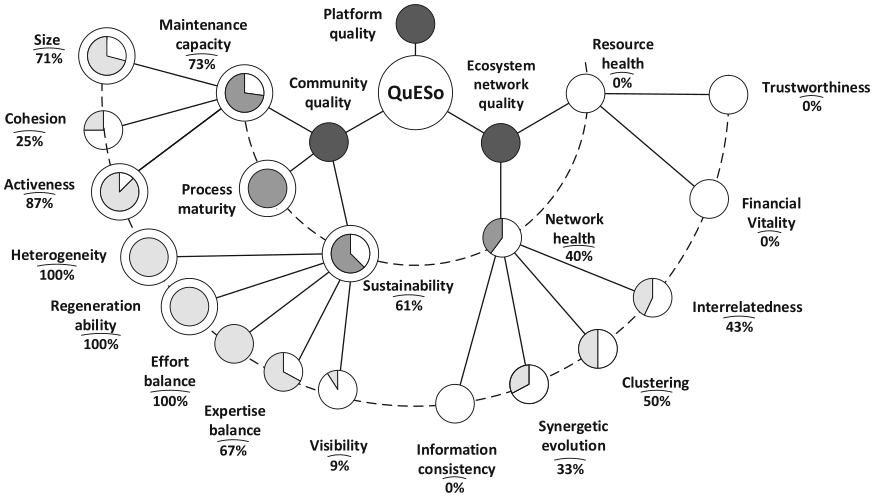
\includegraphics{ábrák/QuESo.pdf}
\caption{Gnome projekt minősítése QuESo minőségbiztosítási
keretrendszerrel Forrás:{[}402{]}}\label{fig:QuESo}
}
\end{figure}

Az általános és több egyedi {[}403, 404{]} megbízhatósági modell mellett
létezik kifejezetten kockázat alapú minősítő rendszer, ilyen például
Siena kockázatmodellje {[}405{]}, illetve célzottan kódbiztonsági
becslést végző modell mint a CodeTrust{[}406{]}.

Érdekes, és egyre elterjedtebb egyedi jelenség a \ref{sec:FS-J-uxc1}
fejezetben már említett ``önminősítés'' jelensége, ahol a projekt
átláthatóságából adódóan a legjobb fejlesztési gyakorlatnak való
megfelelést kötvetlenül ellenőrizni lehet. A megfelelőség informális
biztosítékaként a projektek különféle ``kitűzőket'' -- tulajdonképpen
szabványos logókat -- használhatnak a projekt lapon.

A vizsgált tudományos anyagok és a szerzők egyöntetű véleménye alapján
kimondható, a FLOSS rendszerek minőségének elbírálásához egyedi
keretrendszerek szükségesek, amelyek figyelembe tudják venni a
fejlesztési módszertanból, terjesztési eltérésekből és licencelési
különbségekből származó jellegzetességeket.

\hypertarget{sec:FS-H-I}{%
\subsection{Fejlesztői felhasználás, integráció
(FS-H-I)}\label{sec:FS-H-I}}

FLOSS termékek integrációja jelentősen csökkentheti a fejlesztési
kockázatokat amennyiben a szervezet saját erőből ilyen tevékenységet
végez. A fejlesztéshez és teszteléshez szükséges idő drasztikusan
csökkenhet, a közösség-alapú fejlesztésnél pedig sokan önként
jelentkeznek a fejlesztői munkára {[}79, 253{]}. A FLOSS komponens
felhasználás lehet mérnöki célú (innováció növelő, piacra kerülési időt
csökkentő és karbantartási feladatok redukáló) valamint lehet üzleti
indíttatású (üzleti növekedést segítő, konkurencia hegemóniájának
megtörését célzó, alternatív üzleti lehetőségeket nyitó) {[}407{]}. Az
félkész FLOSS komponensek használata erőforrásokat szabadít fel,
lerövidíti a fejlesztési szakaszt ami által jobb minőségű szoftverek
jöhetnek létre. Ez minden szektorra igaz amelyet az információ
technológiai hatásai elkezdtek átformálni, de különösen erősen
érzékelhető a fogyasztói elektronikai termékek esetén{[}95{]}. A zárt
forrású fejlesztési módszert alkalmazó harmadik féltől származó
komponensek integrációs lehetőségei limitáltak, a FLOSS változatok
lényegében tetszőleges mértékben alakíthatók igény szerint {[}193{]}.
Lenarduzzi et al.~felmérései szerint az integrátorok motivációja
kimutathatóan a testreszabhatóság és egyszerű integrálhatóság felé
tolódik, a korábban mért költséghatékonyság helyett {[}408{]}.

A komponens integráció két elterjed formája az úgynevezett Black-box és
a White-box integráció. Az előbbinél a fejlesztő csak a bináris formát
használja fel, így a kód elemzésére nincs lehetőség. Az utóbbi a forrás
felhasználására utal, ami többnyire csak FLOSS komponensek esetében
lehetséges {[}122{]}. White-box integráció estén lehetőség nyílik az
integrált komponens átalakítására is ami sokszor jelentős előnyt
biztosít ugyanakkor a szabályozott interfész megkerülésre révén bizonyos
kockázatokat is hordoz.

A FLOSS felhasználásának egyik fő motiváló ereje a függetlenség ígérete.
A Szervezet a szállítótól való függetlenedési törekvése során gyakran
felismeri, hogy a nyílt forrást stratégiai eszközként használhatja, így
a szervezet eredményeit vagy új lehetőségeit tekintve vonzóbbnak találja
a FLOSS változatot {[}409{]} vagy előnyösebb alku pozícióba kerül a
szállítóval szemben. Az interneten keresztül könnyen elérhető FLOSS
komponensek használata ma már kétségtelenül stratégiai szerepet tölt be
az iparban. {[}410{]} A nyílt forrású komponens integráció aránya
folyamatosan növekszik, maga az integráció, migráció és jogi kérdések
problémája viszont sok esetben nem megoldott. Egy esetben 3500 java
programozó között végzett felmérés szerint a tipikus java alkalmazások
80\%-a tartalmazott FLOSS komponenseket, ugyanakkor a szervezetek 76\%-a
nem volt képes megfelelően kezelni saját FLOSS felhasználását (2013-as
adat) {[}179{]}. A FLOSS alkalmazás felhasználással ellentétben (lásd:
\ref{sec:FS-H-F} fejezet) komponens integráció tekintetében nem
mutatható ki statisztikailag szignifikáns különbség a kis és nagy
vállalatok között {[}79{]} azaz a nagyvállalatok relatíve szívesebben
használnak FLOSS komponenseket mint termékeket.

A FLOSS komponensek kiválasztásánál a COTS komponenseknél megszokott
módszertan gyakran nem ad elégséges eredményt {[}411{]} és egyedi
metódusokat kell alkalmazni {[}184{]}. A komponens kiválasztása
tekintetében két uralkodó megközelítés létezik. Sokan egyszerűen
rákeresenek a komponensekre az Interneten, míg mások -- elsősorban
kritikus alkalmazások fejlesztése esetén -- FLOSS komponensek
kiválasztására szakosodott portálokat használnak {[}412{]} vagy
vállalkozások szaktudását veszik igénybe. A jó komponens kiválasztás
módszere kritikus szerepet játszik a fejlesztésben, ugyanakkor az alapja
gyakran szubjektív, tapasztalati úton elérhető tudás, így különösen
fontos a megszerzett információk megosztása a közösséggel{[}413{]}. A
kiválasztást végzők többsége egyáltalán nem használ illetve nem is ismer
semmilyen formális módszertant ami a komponens kiválasztási folyamatban
segítséget nyújthatna, ehelyett informális módszerekkel dolgoznak és
sokszor nem is dokumentálják a kiválasztás és döntés indokait és
folyamatát {[}410, 414{]}.

Pedig az integráció egyáltalán nem veszély nélküli folyamat, az
integrátornak számos kihívással szembe kell néznie, a közösségben való
részvételnek ugyanis ára van. Sok gondot okozhat a FLOSS komponensek
közötti koordináció és figyelembe kell venni, hogy az egyes komponensek
kiadási dátuma, frissítési ciklusa, fejlesztési terve eltérő lehet. A
projektnek tehát fel kell készülnie saját és a közösség munkájának
összehangolására. A nyílt forrás felhasználásának tehát meghatározott
``biztonsági költségvonzata'' van {[}160{]}. Stol kutatásaiban
részletesebb felosztást alkalmaz. Az általa azonosított kihívásokat a
\ref{tbl:IntKih} táblázat foglalja össze (az ebben a fejezetben nem
tárgyalt tényezőket a harmadik oszlopban jelölt kategóriánál dolgoztam
fel){[}120{]}.

\hypertarget{tbl:IntKih}{}
\begin{longtable}[]{@{}lll@{}}
\caption{\label{tbl:IntKih}FLOSS integrációja során felmerülő lehetséges
kihívások, Stol nyomán {[}120{]}}\tabularnewline
\toprule
\begin{minipage}[b]{0.24\columnwidth}\raggedright
Kategória\strut
\end{minipage} & \begin{minipage}[b]{0.49\columnwidth}\raggedright
Azonosított kihívás\strut
\end{minipage} & \begin{minipage}[b]{0.18\columnwidth}\raggedright
Fejezet\strut
\end{minipage}\tabularnewline
\midrule
\endfirsthead
\toprule
\begin{minipage}[b]{0.24\columnwidth}\raggedright
Kategória\strut
\end{minipage} & \begin{minipage}[b]{0.49\columnwidth}\raggedright
Azonosított kihívás\strut
\end{minipage} & \begin{minipage}[b]{0.18\columnwidth}\raggedright
Fejezet\strut
\end{minipage}\tabularnewline
\midrule
\endhead
\begin{minipage}[t]{0.24\columnwidth}\raggedright
Termékkiválasztás\strut
\end{minipage} & \begin{minipage}[t]{0.49\columnwidth}\raggedright
A minőségi termék beazonosítása nehéz a bizonytalanság és a nagy számú
variáns miatt\strut
\end{minipage} & \begin{minipage}[t]{0.18\columnwidth}\raggedright
\strut
\end{minipage}\tabularnewline
\begin{minipage}[t]{0.24\columnwidth}\raggedright
.\strut
\end{minipage} & \begin{minipage}[t]{0.49\columnwidth}\raggedright
Nincs idő a komponensek értékelésére\strut
\end{minipage} & \begin{minipage}[t]{0.18\columnwidth}\raggedright
\strut
\end{minipage}\tabularnewline
\begin{minipage}[t]{0.24\columnwidth}\raggedright
.\strut
\end{minipage} & \begin{minipage}[t]{0.49\columnwidth}\raggedright
A megfelelő fork kiválasztása problematikus\strut
\end{minipage} & \begin{minipage}[t]{0.18\columnwidth}\raggedright
\ref{sec:FS-F-P}\strut
\end{minipage}\tabularnewline
\begin{minipage}[t]{0.24\columnwidth}\raggedright
Dokumentáció\strut
\end{minipage} & \begin{minipage}[t]{0.49\columnwidth}\raggedright
Dokumentáció hiánya vagy gyenge minősége\strut
\end{minipage} & \begin{minipage}[t]{0.18\columnwidth}\raggedright
\ref{sec:FS-J-D}\strut
\end{minipage}\tabularnewline
\begin{minipage}[t]{0.24\columnwidth}\raggedright
.\strut
\end{minipage} & \begin{minipage}[t]{0.49\columnwidth}\raggedright
Azonos komponens eltérő leírásokkal\strut
\end{minipage} & \begin{minipage}[t]{0.18\columnwidth}\raggedright
\ref{sec:FS-J-D}\strut
\end{minipage}\tabularnewline
\begin{minipage}[t]{0.24\columnwidth}\raggedright
Közösségi támogatás és karbantartás\strut
\end{minipage} & \begin{minipage}[t]{0.49\columnwidth}\raggedright
Függés a közösségtől támogatás és frissítések terén, a támogatás
minősége nehezen irányítható, nincs helpdesk vagy technikai
segítség\strut
\end{minipage} & \begin{minipage}[t]{0.18\columnwidth}\raggedright
\ref{sec:FS-T-T}\strut
\end{minipage}\tabularnewline
\begin{minipage}[t]{0.24\columnwidth}\raggedright
.\strut
\end{minipage} & \begin{minipage}[t]{0.49\columnwidth}\raggedright
Az egyedi változtatásokat karban kell tartani, ami időigényes és a
jövőbeli változatokkal összeütközésbe kerülhet\strut
\end{minipage} & \begin{minipage}[t]{0.18\columnwidth}\raggedright
\strut
\end{minipage}\tabularnewline
\begin{minipage}[t]{0.24\columnwidth}\raggedright
.\strut
\end{minipage} & \begin{minipage}[t]{0.49\columnwidth}\raggedright
Az FLOSS közösséget nehéz meggyőzni a változások elfogadásáról, a
részvétel drága és nehézkes. A szerkezetet nehéz irányítani ha nem
vagyunk tagja a core fejlesztők csapatának.\strut
\end{minipage} & \begin{minipage}[t]{0.18\columnwidth}\raggedright
\ref{sec:FS-F-K}\strut
\end{minipage}\tabularnewline
\begin{minipage}[t]{0.24\columnwidth}\raggedright
.\strut
\end{minipage} & \begin{minipage}[t]{0.49\columnwidth}\raggedright
Bizonytalanság a termék jövőjét illetően a cég termékének
vonatkozásában\strut
\end{minipage} & \begin{minipage}[t]{0.18\columnwidth}\raggedright
\strut
\end{minipage}\tabularnewline
\begin{minipage}[t]{0.24\columnwidth}\raggedright
.\strut
\end{minipage} & \begin{minipage}[t]{0.49\columnwidth}\raggedright
A közösség tagjai nagyobb beleszólást akarnak a termék tervezett
funkcionalitásába\strut
\end{minipage} & \begin{minipage}[t]{0.18\columnwidth}\raggedright
\strut
\end{minipage}\tabularnewline
\begin{minipage}[t]{0.24\columnwidth}\raggedright
.\strut
\end{minipage} & \begin{minipage}[t]{0.49\columnwidth}\raggedright
A FLOSS projektbe belépés és fejlesztés plusz erőforrásokat
igényel\strut
\end{minipage} & \begin{minipage}[t]{0.18\columnwidth}\raggedright
\strut
\end{minipage}\tabularnewline
\begin{minipage}[t]{0.24\columnwidth}\raggedright
Integráció és szerkezeti felépítés\strut
\end{minipage} & \begin{minipage}[t]{0.49\columnwidth}\raggedright
Visszamenőleges kompatibilitási problémák\strut
\end{minipage} & \begin{minipage}[t]{0.18\columnwidth}\raggedright
\strut
\end{minipage}\tabularnewline
\begin{minipage}[t]{0.24\columnwidth}\raggedright
.\strut
\end{minipage} & \begin{minipage}[t]{0.49\columnwidth}\raggedright
Hiányzó képességek vagy a keretrendszerhez való illesztés miatt
módosításokat kell eszközölni.\strut
\end{minipage} & \begin{minipage}[t]{0.18\columnwidth}\raggedright
\strut
\end{minipage}\tabularnewline
\begin{minipage}[t]{0.24\columnwidth}\raggedright
.\strut
\end{minipage} & \begin{minipage}[t]{0.49\columnwidth}\raggedright
Inkompatibilitási problémák a meglévő rendszer és a komponensek
között.\strut
\end{minipage} & \begin{minipage}[t]{0.18\columnwidth}\raggedright
\strut
\end{minipage}\tabularnewline
\begin{minipage}[t]{0.24\columnwidth}\raggedright
.\strut
\end{minipage} & \begin{minipage}[t]{0.49\columnwidth}\raggedright
Horizontális integráció.\strut
\end{minipage} & \begin{minipage}[t]{0.18\columnwidth}\raggedright
\strut
\end{minipage}\tabularnewline
\begin{minipage}[t]{0.24\columnwidth}\raggedright
.\strut
\end{minipage} & \begin{minipage}[t]{0.49\columnwidth}\raggedright
Vertikális integráció, platform vagy fejlesztői nyelv eltérése.\strut
\end{minipage} & \begin{minipage}[t]{0.18\columnwidth}\raggedright
\strut
\end{minipage}\tabularnewline
\begin{minipage}[t]{0.24\columnwidth}\raggedright
Migráció és felhasználás\strut
\end{minipage} & \begin{minipage}[t]{0.49\columnwidth}\raggedright
Konfiguráció komplexitása\strut
\end{minipage} & \begin{minipage}[t]{0.18\columnwidth}\raggedright
\ref{sec:FS-J-H}\strut
\end{minipage}\tabularnewline
\begin{minipage}[t]{0.24\columnwidth}\raggedright
.\strut
\end{minipage} & \begin{minipage}[t]{0.49\columnwidth}\raggedright
Felhasználói képzés költsége\strut
\end{minipage} & \begin{minipage}[t]{0.18\columnwidth}\raggedright
\strut
\end{minipage}\tabularnewline
\begin{minipage}[t]{0.24\columnwidth}\raggedright
Jogi és üzleti kérdések\strut
\end{minipage} & \begin{minipage}[t]{0.49\columnwidth}\raggedright
Komplex licencelési szituációk\strut
\end{minipage} & \begin{minipage}[t]{0.18\columnwidth}\raggedright
\ref{sec:FS-SZ-L}\strut
\end{minipage}\tabularnewline
\begin{minipage}[t]{0.24\columnwidth}\raggedright
.\strut
\end{minipage} & \begin{minipage}[t]{0.49\columnwidth}\raggedright
Aggályok vagy stratégia hiánya az IP és jogi kérdésekben\strut
\end{minipage} & \begin{minipage}[t]{0.18\columnwidth}\raggedright
\ref{sec:FS-J-H}\strut
\end{minipage}\tabularnewline
\begin{minipage}[t]{0.24\columnwidth}\raggedright
.\strut
\end{minipage} & \begin{minipage}[t]{0.49\columnwidth}\raggedright
Egyértelmű üzleti modell hiánya ami elfogadható lenne az ipar
számára\strut
\end{minipage} & \begin{minipage}[t]{0.18\columnwidth}\raggedright
\ref{sec:FS-T-L}\strut
\end{minipage}\tabularnewline
\bottomrule
\end{longtable}

Az integráció további veszélyforrása, ha az integrátor nem ismeri a
felhasznált kódbázist így akaratlanul is új hibákat vezethet be. A
komponensek között bonyolult függőségi viszony létezhet, a komponensek
újabb komponensektől függenek, így az azokban rejlő hibák
veszélyeztethetik a felhasznált komponens biztonságát is{[}119{]}. Ezen
kívül, ha a helyi módosítások nem kerülnek be az eredeti kódbázisba,
azokat folyamatosan karban kell tartani, ami erőforrás igényes és
további hibalehetőségeket hordoz {[}119, 125, 415{]}, a komponens
változásait minden egyes verzióváltáskor újra ellenőrizni kell, a
fejlesztést pedig lehetőség szerint szinkronizálni kell a forrás
(upstream) projekttel. A Nokia n800-as táblagépe például nagy számú (428
darab) FLOSS komponenst használt, amelyek jelentős részét
(\textasciitilde50\%) módosították. Felmerül a kérdés, a gyártó hogyan
tudta biztosítani a rendszer stabilitását a módosítások visszavezetése
nélkül.

Minden egyes felhasznált komponens újabb függőséget alakít ki, amely
rejtett karbantartási költséget és biztonsági kockázatot jelent. A
Debian szoftverkönyvtár-csomagoktól például átlagosan 6.4 másik csomag
függ közvetlenül (median: 2.0) és 47.6 tranzitív módon (median: 3.0)
{[}119{]}. Jól demonstrálja a jelenség veszélyeit az OpenSSL csomagban
feltárt biztonsági hiba, amely helyi javításként került a Debian
változatába ahol teljes két éven keresztül (2006-2008) folyamatosan
jelen volt. A kriptográfiai kulcs megfelelő véletlenségét biztosító
függvényt a helyi javítás megjegyzésbe tette {[}123, 416{]}. A
karbantartó kapcsolatba lépett a upstream karbantartókkal, ám mivel nem
fedte fel magát és terveit teljes mértékben, lényegében figyelmen kívül
hagyták. A biztonsági sérülékenység 44 másik csomagra terjedt át
anélkül, hogy a karbantartók vagy a fejlesztők azonosították volna a
hibát.

A függőségek sérülékenységeinek automatizált vizsgálatára napjainkban
már vannak viszonylag használható megoldások, ezekkel részletesebben a
\ref{sec:FS-T-M}. fejezetben foglalkozom.

A kriptográfiai könyvtárak sajnálatosan elterjedt black-box integrációja
egyébként is aggályos, hiszen egyetlen biztonsági hibának széles körű
következményei lehetnek {[}123{]}.

Mint korábban erre felhívtam a figyelmet, a változtatásokat, különösen a
hibajavitásokat vissza kellene vezetni{[}385{]}. Sajnos ezeket a
változtatásokat gyakran nehéz elfogadtatni {[}318, 417{]}. Továbbá a
változások és egyéb fejlesztések visszavezetése sok esetben nincs
megfelelően szabályozva, pedig világosnak kellene lennie, hogy milyen
esetekben és milyen kódot lehet az eredeti projektbe visszajuttatni
{[}415{]}. A nyílttá tett forráskód bizonyos jogi veszélyeket is
hordozhat. Amennyiben a kód nem tisztázott állapotú szellemi terméket
tartalmaz, a publikáló szervezetnek számolnia kell a pereskedés
lehetőségével {[}38{]} ami sértheti a rendelkezésre állást.

Az integráció több szinten is megvalósulhat. Integrálhatunk pár soros
kódot, vagy középszinten komponens osztályokat, metódusokat, vagy
nagyobb skálán teljes fájlokat, funkciókat vagy komplett rendszert.
{[}79{]} A forrás birtokában az integráció sokkal rugalmasabbá válik és
lényegében feloldja a bináris programkönyvtár interfészek mesterséges
határait, viszont egyúttal el is veszítjük ezen interfészek nyújtotta
biztonságot. A könyvtárak fejlesztői általában feltételezik, hogy ezeken
a határokon belül szabadon módosíthatnak bármit, amire ha nem figyelünk
oda kompatibilitási problémákat vagy hibákat vezethetünk be a
rendszerünkbe.

A kontrollálatlan integráció súlyos veszélyforrás is lehet. A népszerű
biztonsági segédszoftverek között igen sok a FLOSS termék {[}418{]}
amelynek felhasználása kapcsán ismert olyan eset, ahol a belső
hálózatban sérülékeny nyílt forrású biztonsági könyvtárakat és
keretrendszereket használnak fel a saját belső alkalmazásaik
fejlesztésénél {[}179{]}.

Összességében a komponens-integráció kapcsán négyféle kockázati tényezőt
lehet megkülönböztetni:

\begin{enumerate}
\def\labelenumi{\arabic{enumi}.}
\tightlist
\item
  komponens kiválasztás kockázata (nem a megfelelő vagy sérülékeny
  változatot építünk be);
\item
  komponens integrációjának kockázata (rosszul integráljuk a
  komponenst);
\item
  komponens karbantartásának kockázata (frissítések, új változatok
  hibákat vezetnek be, megszűnik a támogatás);
\item
  jogi kockázat\footnote{E négy kategória utolsó elemével a szabályozást
    tárgyaló fejezetben foglalkozom (\ref{sec:FS-SZ}).}. {[}388{]}
\end{enumerate}

A nagy számú FLOSS komponenst felhasználó cégeknek szükségük van
valamilyen FLOSS menedzsment keretrendszerre, amely segítségével
kontrollálni tudják a FLOSS felhasználásukat. A menedzsment
keretrendszer követelményei az extenzív FLOSS-felhasználó cégek között
végzett felmérés alapján az alábbiak{[}419{]}:

\begin{enumerate}
\def\labelenumi{\arabic{enumi}.}
\item
  FLOSS komponensek követése és újrahasznosítása:
\item
  Az eszköz azonosítsa a FLOSS komponenseket a kódbázisban;
\item
  segítsen jelenteni a FLOSS komponenseket az architektúra modellben;
\item
  frissítse a FLOSS komponenseket és metaadataikat;
\item
  vezessen nyilvántartást a felhasznált FLOSS komponensekről;
\item
  nyújtson lehetőséget a már egyszer felhasznált komponens
  újrahasznosítására.
\item
  Licenc megfelelőség:
\item
  Az eszköz értelmezze a nyílt licenceket;
\item
  dokumentálja a komponens licencét a szervezet adattárában;
\item
  segítsen keresni az adattárban;
\item
  képes legyen igazolni, hogy a komponens licence megfelel a projekt
  irányának;
\item
  segítsen olyan licenc kiválasztásában ami kompatibilis az integrál
  komponensek licencével.
\item
  FLOSS komponensek keresése és kiválasztása:
\item
  Az eszköz nyújtson lehetőséget a FLOSS komponensek közötti keresésre;
\item
  segítsen megtalálni a legjobb komponenst;
\item
  legyen képes megbecsülni a komponens használatának költségét.
\item
  Egyéb követelmények:
\item
  Az eszköz képes legyen megtalálni és megelőzni a komponensben
  található sérülékenységeket;
\item
  dokumentálja és kommunikálja a cég FLOSS kezelési stratégiáját,
  rendszabályait és javasolt gyakorlatát;
\item
  segítsen a felhasználónak megismerni a FLOSS kezelés és megfelelőség
  elveit a fejlesztés és a közösséggel való kommunikáció során.
\end{enumerate}

Összefoglalva, a FLOSS komponens felhasználás biztonsági problémákat
okozhat, menedzsmentje kihívásokkal teli komplex feladat. Különösen
fontos a bizalom és megbízhatóság, a komponens biztonsági modellezés
kérdése és a tesztelés {[}420{]}. A közösséggel való kommunikáció
nehezen elkerülhető és nem is javasolt. A változásokat lehetőség szerint
vissza kell vezetni a forrásprojektbe, ugyanakkor bizonyos információk
nem oszthatók meg a nyílt forrású közösséggel. Külön figyelmet kell rá
fordítani, hogy ezek az információk ne szivároghassanak ki {[}421{]}.

A téma összetettsége folytán komoly igény mutatkozik a FLOSS komponens
integráció célzott oktatására, hiszen a fejlesztőknek egyre inkább oda
kell figyelniük rá, hogyan tartják a kapcsolatot a FLOSS világával.
{[}119{]}

\hypertarget{sec:FS-H-Gy}{%
\subsection{Gyártófüggetlenség (FS-H-Gy)}\label{sec:FS-H-Gy}}

A FLOSS egyik csábító előnye, hogy felhasználásával csökkenthető, vagy
akár meg is szüntethető a vendor-lock-in jelensége, azaz a szállítóktól,
gyártóktól való függés. Nyílt környezetben nem szükséges elkötelezni
magunkat egyetlen cég vagy környezet mellett sem. Továbbá a FLOSS nem
kényszeríti a szervezetet szoftver és hardverspirálba, ugyanis a régebbi
hardveren is jól használható és a frissítéseket sem követeli meg
{[}187{]}. Bár a biztonsági frissítések nélküli szoftverhasználat komoly
veszélyt jelenthet, bizonyos nyílt projektek (mint minden nagyobb Linux
disztribúció) szabott ideig tisztán biztonsági frissítéseket is
garantálnak, további képesség-fejlesztések kikényszerítése nélkül.

A rendelkezésre álló felmérések {[}189, 195, 422{]} azt mutatták, hogy a
közszolgálati szektorban a gyártóktól való függetlenedés a FLOSS
megoldások egyik legfontosabb előnye. A függetlenség két kulcsfontosságú
pontja, hogy a szervezet ne függjön külső szereplőktől az adatbiztonság
terén és ne kötődjön bizonyos szoftver termékekhez vagy gyártókhoz
{[}15{]}. A kívánt függetlenség elérhető tisztán FLOSS rendszerekkel,
vagy üzleti és nyílt rendszerek kombinálásával illetve nyílt szabványok
használatával.

A FLOSS használatával mérhető módon csökkenthető a gazdasági függőség
{[}193{]}. A függetlenség növekedésével a szervezet nyomást tud
gyakorolni a beszállítókra {[}185{]}.

Bár a függetlenség közvetett módon javítja a biztonságot, hiszen nagyobb
rugalmasságot szélesebb mozgásteret biztosít, közvetlen biztonsági
hatást nem azonosítottam.

\hypertarget{sec:FS-H-F}{%
\subsection{Felhasználói tábor (FS-H-F)}\label{sec:FS-H-F}}

A FLOSS felhasználók eloszlása érdekes mintát mutat. Elterjedt nézet,
hogy a nyílt forrású rendszereket programozók fejlesztik programozóknak
vagy éppen saját maguknak. Ez persze erős általánosítás, de a
feldolgozott kutatások azt mutatják, hogy bizonyos mértékig valóban
létezik ilyen jelenség.

A személyi felhasználók közt többségben vannak azok, akik ``programokat
írnak'' még ha nem is feltétlenül professzionális szinten, hanem saját
céljaik elérése érdekében ami általában valami más, könyvelés,
statisztika, webtervezés, kutatás vagy szórakoztatás {[}423{]}. A
Stack-Overflow kommunikációjának analízise azt mutatta, hogy a
fejlesztők tudatában vannak a FLOSS nyújtotta előnyöknek és könnyebben
állnak át az ilyen megoldásokra {[}368{]}.

A fiatalabb korosztály tagjai statisztikailag hajlamosabbak FLOSS
rendszerek használatára, jobban ismerik azt {[}367{]} ami valószínűsíti,
hogy a FLOSS felhasználószám növelését a fiatalabb rétegen keresztül
lehet megcélozni. {[}162{]} Ezzel szemben az ellenzők általában
tapasztaltabbak, ugyanakkor kevesebb a kapcsolatuk a szabad
szoftverekkel.

Nem meglepő módon a szabad szoftver közösségekben szerepet vállaló
személyek körében nagyobb a FLOSS iránti igény, magasabbra is értékelik
azt {[}424{]} és a felhasználótábor (részhalmaza) gyakran egyben maga a
fejlesztő közösség is {[}92{]}.

Hasonlóan magas a biztonsági szakemberek FLOSS felhasználása. A
információ-biztonsági szakemberek általában megbíznak a FLOSS biztonsági
eszközökben. Ugyanakkor érdekes módon a nagyvállalatok már kevésbé
bíznak a FLOSS biztonsági eszközökben (amiben szerepet játszanak az
alább kifejtett okok) {[}373, 425{]}. Li eredményei azt mutatták, hogy a
felhasználók biztonság-kritikus területeken mindenképpen igen óvatosak,
akár COTS\footnote{Commercial Off-The-Self : dobozos termékek, nem
  helyi, egyedi megoldások.} akár FLOSS termékről van szó, a szoftverek
biztonsági aspektusát így nem igazán lehet megkülönböztetni. {[}90{]}

A szervezeti felhasználók közt a magukat innovatívnak tartók
hajlamosabbak kihasználni a FLOSS nyújtotta lehetőségeket és nagyobb
eséllyel jelölik meg jövőbeli célként {[}98{]}. A FLOSS-használó
szervezetek általában kicsik és kevésbé kritikus IT részleggel
rendelkeznek mint a FLOSS-t nem vagy kisebb mértékben használó
vállalkozások. Ez bizonyos értelemben ellentmond annak nézetnek, hogy az
IT szempontból kritikusabb, nagyobb vállalkozások fogékonyabbak az
innovációra. A jelenség oka az lehet, hogy a kis vállalkozások az
alacsony költség miatt ugródeszkaként használhatják a FLOSS
rendszereket, hiszen így gyorsan (és olcsón) hozzájuthatnak a
legfrissebb technológiákhoz. Ugyanakkor a támogatás és a szolgáltatás
körüli bizonytalanságok miatt a nagyobb vállalatok felelős vezetői
inkább kockázatkerülő magatartást követnek {[}426{]}. A mikro és
kisvállalkozások a fejlődőfélben lévő FLOSS leggyakoribb támogatói.
Gyakran járulnak hozzá a projektekhez, ugyanakkor a méretük miatt ők
tudnak a legkevesebbet gazdaságilag profitálni a szabad szoftverekből,
számukra tehát elsősorban a korábban említett ``gyors-rajt'' effektus
biztosítja az előnyt. A középvállalkozások kisebb mértékben de
hajlandóak kísérletezni fejlődőfélben lévő szabad szoftverekkel, sőt
bizonyos esetekben saját szaktudásukat vissza is forgatják a közösség
javát szolgálva. A nagyvállalatok általában biztosra mennek és kizárólag
a bejáratott, érett megoldásokat hajlandóak felhasználni, amelyek
jelentős ideje vannak a piacon és amelyek esetén a biztonsági kockázat a
lehető legkisebb. A nagyvállalatok tehát elsősorban erőforrás
optimalizálás céljából veszik igénybe a FLOSS termékeket {[}427{]}.

Érdekes módon Spinellis statisztikai elemzése azt mutatta, hogy a
gyorsan fejlődő vállaltok és a különösen termelékeny munkavállalók
egyáltalán nem részesítik előnyben a FLOSS rendszereket, sőt, ennek épp
ellenkezője igaz {[}9{]}. Az eredmény csak első látásra meglepő, hiszen
a szabad szoftver erősségének számító testreszabhatóság (lásd alább) nem
nyújt valódi előnyt, ha a piaci termékek -- igaz magasabb árért --
gyorsabban és hatékonyabban le tudják fedni az összes igényt. Ezt pedig
mindig megtehetik akár a FLOSS termék vagy annak komponenseinek
felhasználásával is. A szabad szoftvereknek tehát továbbra is az
alacsony költség marad mint versenyelőny.

\hypertarget{sec:FS-H-P}{%
\subsection{Jellemző piaci szegmensek (FS-H-P)}\label{sec:FS-H-P}}

A FLOSS termékek nem egyformán vannak jelen az egyes piaci területeken.
A FLOSS jelenség jellemzően erős az IT szektorban. Jól ismert
zászlóshajókat találhatunk itt az operációs rendszerek, webkiszolgálók,
böngészők, szoftverfejlesztés, verziókezelés és adatbázis-kezelők
piacán. {[}368{]} Hasonlóképpen erős a jelenléte a middleware {[}416{]},
bioinformatika, katonai számítások és az akadémiai kutatások terén
{[}428{]} sőt bizonyos területeket akár teljesen uralhat is {[}429,
430{]}. Ezek közül a felhőtechnológia különösen figyelemre méltó, hiszen
a FLOSS potenciális problémái a felette futó rendszer sértetlenségét is
veszélyeztetik{[}431, 432{]}.

Érdekes módon a magában is gyakran Létfontosságú Rendszerelemnek számító
közszféra információs rendszereiben növekvő érdeklődés tapasztalható a
FLOSS rendszerek iránt. Míg korábban elsősorban a FLOSS
webszolgáltatásokat használták a szabványkövetés, módosíthatóság és
függetlenség nagy vonzerőt jelentenek ebben a szektorban. {[}15, 195{]}
Ebben a szektorban a polgárok jogai odáig is terjedhetnek, hogy az
adatok előállításának pontos módszereit is megismerhessék, ami a forrás
nyíltsága nélkül aggályos {[}15{]}. A FLOSS jelentősége egyértelműen
növekszik például az Egyesült Királyság közszolgálati szektorában, a
politika egyre inkább felismeri az előnyös hatásokat {[}15{]}.
Belgiumban Viseur erős jelenlétet azonosított a voip, erp és a képzés
terén is{[}433{]}. A globális gazdasági hatás előnyeivel a vonatkozó
részben foglalkozom (\ref{sec:FS-G-G}).

Más területeken ugyanakkor nincs vagy csak elvétve található jó minőségű
(vagy akár minimálisan versenyképes) megoldás. Nincs értékelhető
jelenlét például az ipari célszoftverek piacán {[}422{]} illetve a
tervezőszoftverek területén is, ahol ugyan vannak megoldások de
elmaradnak a piacvezető termékek mögött {[}434{]}. Jellemző a FLOSS
használat az ad-hoc biztonsági megoldások kialakításakor és a
tesztelések során, jelentős szerepet játszik az esemény utáni szakértői
elemzésekben\footnote{Angol nevén ``Forensic Analysis''}, ugyanakkor a
kritikus rendszerekhez már szinte minden esetben üzleti alkalmazásokat
használnak a nagyvállalati szektorban {[}375{]}.

Bizonyos biztonságkritikus területek kifejezetten kerülik a nyíltsággal
járó kockázatokat. Ilyen a DRM\footnote{Digital Right Management}
védelem, az ATM és POS terminálok vagy a smart card ipar
területei{[}435{]}.

\hypertarget{sec:FS-H-A}{%
\subsection{Adatmigráció (FS-H-A)}\label{sec:FS-H-A}}

A FLOSS változatra való áttérés általában nem pusztán egy új szoftver
telepítését jelenti. A meglévő adatokat migrálni kell, a rendszer más
komponensekre irányuló interfészeit újra kell írni. Ez különösen
nehézkes lehet a FLOSS diszkriminatív tulajdonsága miatt (lásd még:
\ref{sec:FS-SZ-L} fejezet). {[}135{]}

Egy esetleges migráció során szervezeti problémákkal is szembe kell
nézni. A vállalati vezetők a változással szembeni ellenállást, a házon
belüli FLOSS szakértelem hiányát és a FLOSS bevezetésével kapcsolatos
tapasztalatok hiányát jelölték meg fő akadályként. {[}135{]}

A nagyvállalatok komplex információs rendszereiben a két legjelentősebb
egyedi érték az idők során létrehozott kifinomult algoritmusok és az azt
karbantartó kompetens csapat. Az algoritmusok és eljárások általában
igen nagy mennyiségű kód integráns részét képezik, amelynek változtatása
meglehetősen nehéz. A hosszú idő alatt felépített csapat és az
összegyűjtött know-how csak lassú változásokra képes. Nem meglepő, hogy
a felső vezetés a rendszer két legfontosabb értékét nem szívesen
kockáztatja, ha úgy érzi a FLOSS bevezetése veszélyeztetné őket.
{[}259{]}

Tekintve, hogy a migrációs folyamat nem mindig visszafordítható, a
migrálás az integritást sértő esetleges migrációs hibáktól eltekintve is
sértheti a rendelkezésre állást elvét, tekintve, hogy a migrálás előtti
rendszermentések az újr rendszerbe csak komoly nehézségek árán tölthetők
vissza.

\hypertarget{sec:FS-H-T}{%
\subsection{Egyedi igényekhez alakíthatóság, testreszabás
(FS-H-T)}\label{sec:FS-H-T}}

A szoftvergyártó-felhasználó értékesítési csatornában a legtöbb esetben
megjelennek köztes szereplők, az úgynevezett rendszerintegrátorok. A
gyártó nem közvetlenül értékesíti termékét, hanem a rendszerintegrátoron
keresztül, melynek termékében központi komponens az adott szoftver, de
kiegészítő termékeket és szolgáltatásokat kínál hozzá. A jó minőségű
szoftverrendszer előállításánál a FLOSS szinte teljes mértékű
módosíthatósága nagy előnyt jelent, hiszen a forráskód birtokában elvben
bármilyen átalakítás elvégezhető {[}188{]}. A forrás módosításával olyan
egyedi biztonsági lehetőségek nyílnak meg, amelyek elképzelhetetlenek
zárt forrás esetén. Ilyen lehet például a jogosultsági szint emelés
alapú támadások (privilege escalation) automatikus elemzése {[}436{]}.

Egyes vásárlóknak olyan speciális igényei lehetnek, amelyeket a
szabványos változattal nem lehet kielégíteni, a kód változtatásának
lehetősége pedig megoldást jelenthet erre a problémára, ami az
integrátorok számára különösen előnyös. {[}38{]} Az fejlesztők számára
egyetlen késztermék átalakítása kisebb befektetéssel jár hasonló
eredmények mellett, mint egy teljesen új termék létrehozása. Teljes
funkciókhoz jutnak így ingyenesen, a hiányzó képességeket már könnyebb
pótolni. {[}200{]} A lokalizáció, azaz a helyi nyelvhez, szokásokhoz
illesztés is könnyebben elvégezhető ha a forrás és a fordítást végző
közösség rendelkezésre áll. Ez a képesség a FLOSS rendszerek egyik
erőssége {[}135{]} bár a lokalizációt célzó SaaS
szolgáltatások\footnote{ilyen SaaS szolgáltatást nyújt például a
  Transifex (https://www.transifex.com/)} részlegesen csökkenthetik az
üzleti szoftverrendszer lokalizációs terheit, az azonnali és egyedi
módosítás továbbra is csak a forrás birtokában lehetséges.

A nyílt kód segítségével egyúttal magasabb biztonsági szint is elérhető,
hiszen az esetleges hibák és biztonsági rések kijavíthatóak {[}187{]}. A
változtatásokat saját időbeosztás szerint bármikor el lehet végezni, nem
kell várakozni a gyártó kiadási ciklusaira {[}80{]}. A zárt forrású
megoldásokba nem lehet belenyúlni, vészhelyzetben nincs lehetőség a
reakcióra, az egyetlen azonnali megoldás a folyamat ismételt
újraindítása ami nem feltétlenül vezet eredményre. Nyílt forrás esetén
megfelelő szaktudás mellett legalább a lehetőség adott {[}56{]}.

A felhasználók szemszögéből nézve a testreszabhatóság kérdése
árnyaltabb. Az üzleti megoldások általában rendelkeznek valamilyen
szintű beállítási lehetőséggel, de a FLOSS rendszerek testreszabási
lehetőségei messze meghaladják ezeket {[}114{]}. Problémát jelent
viszont, hogy a testreszabáshoz általában jelentős szakismeret és idő
szükséges, ami egy átlagfelhasználó esetén sokszor túlzó elvárás. Ezt
igazolták Spinellis korábban említett eredményei, amelyből látható, hogy
a gyorsan fejlődő, produktív felhasználók és cégek inkább a piac által
számukra előre testreszabott megoldásokat részesítik előnyben. {[}9{]}

A változtathatóság előnyeinek pontos értékét azonban nem könnyű
felbecsülni {[}80{]} a változtatásnak pedig adminisztrációs ára van. Az
új verziók változásait a szervezetnek követni kell, ha nem akar
lemondani a biztonsági frissítések nyújtotta előnyökről. Amennyiben nem
vezeti vagy nem tudja visszavezetni a változtatásait {[}437, 438{]} a
közösség támogatása jelentősen csökkenhet ha később problémák merülnek
fel. A javítások visszavezetése során fontos a közösség által elvárt
szociális normák betartása, ellenkező esetben a javítást elutasíthatják
{[}439{]}. A fentiek miatt a változtatás kizárólag indokolt esetben
javasolt. {[}385, 440{]}

Összefoglalva, a testreszabhatóság elsősorban az integrátorok és
fejlesztők számára nyújt valódi előnyöket, a végfelhasználó csak akkor
tudja kiaknázni ezeket a lehetőségeket, ha magasan képzett és megfelelő
mennyiségű idő áll rendelkezésére. Amennyiben a szervezet belső
erőforrásból végez rendszer-fejlesztéseket a testreszabhatóság jelenthet
biztonsági előnyt, egyéb esetben ez a hatás nem releváns.

\begin{longtable}[]{@{}rcll@{}}
\caption{A \emph{H} kategóriában azonosított problémák}\tabularnewline
\toprule
\begin{minipage}[b]{0.03\columnwidth}\raggedleft
kód\strut
\end{minipage} & \begin{minipage}[b]{0.03\columnwidth}\centering
szint\strut
\end{minipage} & \begin{minipage}[b]{0.69\columnwidth}\raggedright
leírás\strut
\end{minipage} & \begin{minipage}[b]{0.13\columnwidth}\raggedright
sajátosság\strut
\end{minipage}\tabularnewline
\midrule
\endfirsthead
\toprule
\begin{minipage}[b]{0.03\columnwidth}\raggedleft
kód\strut
\end{minipage} & \begin{minipage}[b]{0.03\columnwidth}\centering
szint\strut
\end{minipage} & \begin{minipage}[b]{0.69\columnwidth}\raggedright
leírás\strut
\end{minipage} & \begin{minipage}[b]{0.13\columnwidth}\raggedright
sajátosság\strut
\end{minipage}\tabularnewline
\midrule
\endhead
\begin{minipage}[t]{0.03\columnwidth}\raggedleft
SH01\strut
\end{minipage} & \begin{minipage}[t]{0.03\columnwidth}\centering
1\strut
\end{minipage} & \begin{minipage}[t]{0.69\columnwidth}\raggedright
A szervezet nem megfelelő minősítő rendszert alkalmaz a FLOSS termék
minősítésére.\strut
\end{minipage} & \begin{minipage}[t]{0.13\columnwidth}\raggedright
FS-H-M\strut
\end{minipage}\tabularnewline
\begin{minipage}[t]{0.03\columnwidth}\raggedleft
SH02\strut
\end{minipage} & \begin{minipage}[t]{0.03\columnwidth}\centering
1\strut
\end{minipage} & \begin{minipage}[t]{0.69\columnwidth}\raggedright
Megfelelő változat kiválasztása nehéz és időigényes. Emiatt
előfordulhat, hogy nem a megfelelő változat kerül alkalmazásra.\strut
\end{minipage} & \begin{minipage}[t]{0.13\columnwidth}\raggedright
FS-H-M\strut
\end{minipage}\tabularnewline
\begin{minipage}[t]{0.03\columnwidth}\raggedleft
SH03\strut
\end{minipage} & \begin{minipage}[t]{0.03\columnwidth}\centering
2\strut
\end{minipage} & \begin{minipage}[t]{0.69\columnwidth}\raggedright
A kontroll nélküli (esetleg rejtett) integráció a hibás komponensek
révén sérülékenységek akaratlan beépítéséhez vezet.\strut
\end{minipage} & \begin{minipage}[t]{0.13\columnwidth}\raggedright
FS-H-I\strut
\end{minipage}\tabularnewline
\begin{minipage}[t]{0.03\columnwidth}\raggedleft
SH04\strut
\end{minipage} & \begin{minipage}[t]{0.03\columnwidth}\centering
1\strut
\end{minipage} & \begin{minipage}[t]{0.69\columnwidth}\raggedright
A FLOSS komponensek minősítésére nem alkalmas a COTS esetén megszokott
módszertan.\strut
\end{minipage} & \begin{minipage}[t]{0.13\columnwidth}\raggedright
FS-H-M\strut
\end{minipage}\tabularnewline
\begin{minipage}[t]{0.03\columnwidth}\raggedleft
SH05\strut
\end{minipage} & \begin{minipage}[t]{0.03\columnwidth}\centering
2\strut
\end{minipage} & \begin{minipage}[t]{0.69\columnwidth}\raggedright
Az integrátor nem ismeri megfelelő mélységben az integrálandó komponenst
így hibákat vezet be az integráció során.\strut
\end{minipage} & \begin{minipage}[t]{0.13\columnwidth}\raggedright
FS-H-M\strut
\end{minipage}\tabularnewline
\begin{minipage}[t]{0.03\columnwidth}\raggedleft
SH06\strut
\end{minipage} & \begin{minipage}[t]{0.03\columnwidth}\centering
3\strut
\end{minipage} & \begin{minipage}[t]{0.69\columnwidth}\raggedright
Az integrált komponensen végzett módosítások összeütközésbe kerülnek az
eredeti kódbázissal, ami a frissítések során hibákhoz vagy
sérülékenységhez vezethet.\strut
\end{minipage} & \begin{minipage}[t]{0.13\columnwidth}\raggedright
FS-H-T\strut
\end{minipage}\tabularnewline
\begin{minipage}[t]{0.03\columnwidth}\raggedleft
SH07\strut
\end{minipage} & \begin{minipage}[t]{0.03\columnwidth}\centering
4\strut
\end{minipage} & \begin{minipage}[t]{0.69\columnwidth}\raggedright
A szükséges módosításokat nem sikerül visszavezetni, a közösség
elutasítja így a kódbázis ütközéseit folyamatosan figyelni kell, ami
időigényes és hibalehetőségekkel terhelt.\strut
\end{minipage} & \begin{minipage}[t]{0.13\columnwidth}\raggedright
FS-H-M\strut
\end{minipage}\tabularnewline
\begin{minipage}[t]{0.03\columnwidth}\raggedleft
SH08\strut
\end{minipage} & \begin{minipage}[t]{0.03\columnwidth}\centering
1\strut
\end{minipage} & \begin{minipage}[t]{0.69\columnwidth}\raggedright
Az integrált komponens összetett függőségein keresztül hibás (és
ellenőrizetlen) alkomponensek szivároghatnak a fejlesztésbe.\strut
\end{minipage} & \begin{minipage}[t]{0.13\columnwidth}\raggedright
FS-H-M\strut
\end{minipage}\tabularnewline
\begin{minipage}[t]{0.03\columnwidth}\raggedleft
SH09\strut
\end{minipage} & \begin{minipage}[t]{0.03\columnwidth}\centering
4\strut
\end{minipage} & \begin{minipage}[t]{0.69\columnwidth}\raggedright
A módosítások visszavezetése során érzékeny információ szivárog ki az
upstream projektbe.\strut
\end{minipage} & \begin{minipage}[t]{0.13\columnwidth}\raggedright
FS-H-M\strut
\end{minipage}\tabularnewline
\begin{minipage}[t]{0.03\columnwidth}\raggedleft
SH10\strut
\end{minipage} & \begin{minipage}[t]{0.03\columnwidth}\centering
1\strut
\end{minipage} & \begin{minipage}[t]{0.69\columnwidth}\raggedright
Kompatibilitási problémák miatt a szervezet által alkalmazott
felügyeleti rendszer nem támogatja a FLOSS változatot.\strut
\end{minipage} & \begin{minipage}[t]{0.13\columnwidth}\raggedright
-\strut
\end{minipage}\tabularnewline
\begin{minipage}[t]{0.03\columnwidth}\raggedleft
SH11\strut
\end{minipage} & \begin{minipage}[t]{0.03\columnwidth}\centering
1\strut
\end{minipage} & \begin{minipage}[t]{0.69\columnwidth}\raggedright
A szükséges adatmigrációt követően a korábbi mentések helyreállítása
nehézzé vagy lehetetlenné válik, veszélyeztetve a rendelkezésre
állást.\strut
\end{minipage} & \begin{minipage}[t]{0.13\columnwidth}\raggedright
FS-H-A\strut
\end{minipage}\tabularnewline
\bottomrule
\end{longtable}

\begin{longtable}[]{@{}rcll@{}}
\caption{A \emph{H} kategóriában azonosított javaslatok}\tabularnewline
\toprule
\begin{minipage}[b]{0.03\columnwidth}\raggedleft
kód\strut
\end{minipage} & \begin{minipage}[b]{0.03\columnwidth}\centering
szint\strut
\end{minipage} & \begin{minipage}[b]{0.69\columnwidth}\raggedright
leírás\strut
\end{minipage} & \begin{minipage}[b]{0.13\columnwidth}\raggedright
probléma\strut
\end{minipage}\tabularnewline
\midrule
\endfirsthead
\toprule
\begin{minipage}[b]{0.03\columnwidth}\raggedleft
kód\strut
\end{minipage} & \begin{minipage}[b]{0.03\columnwidth}\centering
szint\strut
\end{minipage} & \begin{minipage}[b]{0.69\columnwidth}\raggedright
leírás\strut
\end{minipage} & \begin{minipage}[b]{0.13\columnwidth}\raggedright
probléma\strut
\end{minipage}\tabularnewline
\midrule
\endhead
\begin{minipage}[t]{0.03\columnwidth}\raggedleft
JH01\strut
\end{minipage} & \begin{minipage}[t]{0.03\columnwidth}\centering
1\strut
\end{minipage} & \begin{minipage}[t]{0.69\columnwidth}\raggedright
Formális tanúsítás híján a felhasznált komponensek kódját megbízhatósági
modellekkel kell vizsgálni (pl. CodeTrust).\strut
\end{minipage} & \begin{minipage}[t]{0.13\columnwidth}\raggedright
SF05, SH01, SH02\strut
\end{minipage}\tabularnewline
\begin{minipage}[t]{0.03\columnwidth}\raggedleft
JH02\strut
\end{minipage} & \begin{minipage}[t]{0.03\columnwidth}\centering
3\strut
\end{minipage} & \begin{minipage}[t]{0.69\columnwidth}\raggedright
A kód szabad módosíthatósága miatt várakozás nélkül javíthatóak a
sérülékenységek, amennyiben a kód módosításához szükséges erőforrás és
szakismeret rendelkezésre áll.\strut
\end{minipage} & \begin{minipage}[t]{0.13\columnwidth}\raggedright
\strut
\end{minipage}\tabularnewline
\begin{minipage}[t]{0.03\columnwidth}\raggedleft
JH04\strut
\end{minipage} & \begin{minipage}[t]{0.03\columnwidth}\centering
2\strut
\end{minipage} & \begin{minipage}[t]{0.69\columnwidth}\raggedright
A felhasználandó FLOSS komponenseket erre szakosodott szakértők révén
szerezzük be.\strut
\end{minipage} & \begin{minipage}[t]{0.13\columnwidth}\raggedright
SF05, SH04, SH05, SH08, SJ01, SM06\strut
\end{minipage}\tabularnewline
\begin{minipage}[t]{0.03\columnwidth}\raggedleft
JH05\strut
\end{minipage} & \begin{minipage}[t]{0.03\columnwidth}\centering
1\strut
\end{minipage} & \begin{minipage}[t]{0.69\columnwidth}\raggedright
A FLOSS komponens kiválasztásának folyamatát és körülményeit
dokumentálni kell.\strut
\end{minipage} & \begin{minipage}[t]{0.13\columnwidth}\raggedright
SF05, SF10, SH05\strut
\end{minipage}\tabularnewline
\begin{minipage}[t]{0.03\columnwidth}\raggedleft
JH06\strut
\end{minipage} & \begin{minipage}[t]{0.03\columnwidth}\centering
4\strut
\end{minipage} & \begin{minipage}[t]{0.69\columnwidth}\raggedright
A kód változásait lehetőség szerint vissza kell vezetni az eredeti
projektbe.\strut
\end{minipage} & \begin{minipage}[t]{0.13\columnwidth}\raggedright
SF07, SF11, SH06\strut
\end{minipage}\tabularnewline
\begin{minipage}[t]{0.03\columnwidth}\raggedleft
JH07\strut
\end{minipage} & \begin{minipage}[t]{0.03\columnwidth}\centering
3\strut
\end{minipage} & \begin{minipage}[t]{0.69\columnwidth}\raggedright
A fejlesztést végző részlegnek legyen megfelelő verzió-követési
terve.\strut
\end{minipage} & \begin{minipage}[t]{0.13\columnwidth}\raggedright
SF07, SF10, SF13, SH06\strut
\end{minipage}\tabularnewline
\begin{minipage}[t]{0.03\columnwidth}\raggedleft
JH08\strut
\end{minipage} & \begin{minipage}[t]{0.03\columnwidth}\centering
3\strut
\end{minipage} & \begin{minipage}[t]{0.69\columnwidth}\raggedright
A beszállító vagy a fejlesztést végző részleg alkalmazzon FLOSS
komponens kezelő keretrendszert.\strut
\end{minipage} & \begin{minipage}[t]{0.13\columnwidth}\raggedright
SF07, SF10, SF13, SH03, SH06, SH08, SS02, SS03\strut
\end{minipage}\tabularnewline
\begin{minipage}[t]{0.03\columnwidth}\raggedleft
JH10\strut
\end{minipage} & \begin{minipage}[t]{0.03\columnwidth}\centering
4\strut
\end{minipage} & \begin{minipage}[t]{0.69\columnwidth}\raggedright
A forráskódban minden nem publikus információ világosan definiált
legyen. A változások visszavezetésekor automatizált rendszerrel meg kell
akadályozni a minősített információ kiszivárgását.\strut
\end{minipage} & \begin{minipage}[t]{0.13\columnwidth}\raggedright
SF07, SH09\strut
\end{minipage}\tabularnewline
\begin{minipage}[t]{0.03\columnwidth}\raggedleft
JH11\strut
\end{minipage} & \begin{minipage}[t]{0.03\columnwidth}\centering
2\strut
\end{minipage} & \begin{minipage}[t]{0.69\columnwidth}\raggedright
Képzésekkel kell tudatosítani a komponens integrációval járó veszélyeket
és a biztonságos felhasználáshoz szükséges eljárásokat\strut
\end{minipage} & \begin{minipage}[t]{0.13\columnwidth}\raggedright
SF13, SH04, SH05, SH06, SH08, SH09\strut
\end{minipage}\tabularnewline
\bottomrule
\end{longtable}

\hypertarget{sec:FS-SZ}{%
\section{Szabályozás, megfelelőség (FS-Sz)}\label{sec:FS-SZ}}

Az alfejezetben a FLOSS szabályozással kapcsolatos kérdéseit tárgyalom.
Szabályozás alatt itt az angol ``compliance'' kifejezésnek megfelelő
fogalmat értem, tehát a külső és belső szabályoknak, irányelveknek,
házirendeknek és jogszabályoknak való komplex megfelelést.

A megfelelőségi keretrendszerek (COBIT) illetve szabványok (NIST,
ISO27000) korlátozott használhatósága a minősítő rendszerekkel rokon
problémakör, amellyel a Felhasználás fejezet alatt foglalkozom
(\ref{sec:FS-F-M}. fejezet).

\hypertarget{sec:FS-SZ-B}{%
\subsection{Belső szabályozás (FS-SZ-B)}\label{sec:FS-SZ-B}}

Talán a mikrovállalatokat kivéve minden szervezetnek, legyen az kicsi
vagy nagy, szüksége van valamilyen belső IT szabályozásra részben a jogi
elvárások teljesítése végett, részben mert csak így biztosítható az
működtetéssel járó kockázat elfogadható szintre csökkentése és az elvárt
biztonsági szint fenntartása. Különösen fontos ez a Létfontosságú
Információs Rendszerelemek területén, ahol jogszabályban rögzített
szigorú technológiai és szervezési elvárásoknak kell megfelelni.

Ezek a belső szabályzatok gyakran figyelmen kívül hagyják a FLOSS egyedi
jellegzetességeit, egyáltalán nem, vagy csak ritkán szabályozzák
részletesen a szabad szoftverekkel és nyílt forrású komponensekkel
történő kapcsolattartás módszereit, ami biztonsági és üzleti kockázatot
jelenthet.

Minthogy a FLOSS tekintetében jogszabályok nem írnak elő kötelező belső
szabályozást, a definiálás során döntő szempont a menedzsment
tudatosságának kérdése {[}349{]}. Sajnálatos módon kevés a FLOSS
orientált szabvány, a komponensekkel kapcsolatos nagy mennyiségű,
részleges, diverz és szubjektív információ nem igazán segíti elő a
tudatos döntést {[}413{]}.

Kemp szerint {[}441{]} a nyílt forrású szabályozás célja -- más IP
jellegű szabályozáshoz hasonlóan -- a felesleges viták elkerülése,
vásárlói elégedettség biztosítása és a források megfelelő menedzselése.
A FLOSS szabályozás öt területet kell lefedjen:

\begin{enumerate}
\def\labelenumi{\arabic{enumi}.}
\tightlist
\item
  Beszerzés: milyen FLOSS rendszereket használ a szervezet;
\item
  Megbízható források: ismerni kell honnan származik a FLOSS;
\item
  Követés: ismerni kell, mit csinál, hol használjuk és hol hasznosítjuk
  újra;
\item
  Szerepek és felelősség: tudni kell kinek mi a szerepe és miért felelős
  a FLOSS kapcsán; és
\item
  Licenc megfelelőség: ismerni kell, hogy a szervezet megfelel-e az OSS
  licencekben megjelenő kötelezettségeknek.
\end{enumerate}

Ideális esetben a szabályzat kitér a:

\begin{itemize}
\tightlist
\item
  személyi kérdésekre, egyértelműen megfogalmazva az egyes résztvevők
  szerepköreit és céljait ;
\item
  felállít egy követendő globális stratégiát, ide értve az üzleti,
  kockázatkezelési és IP stratégiákat ;
\item
  foglalkozik a házirend kérdésével, amelynek tömörnek, egyértelműnek
  esemény orientáltnak kell lennie, kritériumokat és döntési pontokat
  kell megfogalmaznia az FLOSS felhasználása terén, és egyértelművé kell
  tenni a gyűjtendő és követendő információkat;
\item
  definiálja a folyamatokat, ahol meg kell fogalmazni a más területek
  szabályozásával kapcsolatos függőségeket, kitér a projekt-tervezéssel,
  kivitelezéssel és utókövetéssel kapcsolatos kérdésekre, illetve
  érdemes megfontolni a FLOSS közösség bevonását és megnyerését célzó
  alfolyamatok létrehozását is;
\item
  foglalkozik a sérülékenységek kezelésével.
\end{itemize}

Sajnálatos módon ezeket az elveket kevés szervezet követi a
gyakorlatban. A legtöbb esetben ad-hoc módon hoznak döntéseket,
pragmatikus, használat orientált módon amely nem vesz figyelembe sem
költséghatékonyságot sem más magasabb rendű stratégiát {[}376{]}.

\hypertarget{sec:FS-SZ-L}{%
\subsection{Összetett licencelés (FS-SZ-L)}\label{sec:FS-SZ-L}}

A FLOSS licenckörnyezete meglehetősen összetett. Számtalan szabad
licenctípus létezik, amely több vagy kevesebb korlátozást tartalmaz
illetve eltérő jogokkal ruházza fel a felhasználót. A szervezetek
számára legvonzóbb ilyen jog a jogátruházás lehetősége, amely lehetővé
teszi, hogy az üzleti licencek hagyományos EULA\footnote{End User
  License Agreement, magyarul Végfelhasználói licencszerződés, vagy
  másképp végfelhasználói engedély.} szakaszával ellentétben a terméket
ne csak használhassuk hanem lemásolhassuk és akár el is adhassuk {[}356,
442{]}. Az OSI\footnote{Open Source Initiative, nyílt forrású licencek
  OSD (Open Source Definition) kompatibilitásának tanúsítást végző
  szervezet. https://opensource.org/} jelenleg (2018 augusztusa) 83 OSS
licencet listáz, amely segítséget nyújthat a különféle licencek közötti
eligazodásban {[}152{]}. A licenceket két alapvető csoportra, a
megengedő (Permissive) és kötött (Restrictive) licenctípusok körére
szokás bontani. Mindkét licenccsoport tagjai tartalmazzák a nyílt
szoftverekre jellemző alapvető jogokat -- a forrás elérhetőségét, szabad
módosíthatóságát és a jogátruházás képességét -- a korlátozások
tekintetében viszont más feltételeket fogalmaznak meg. Leegyszerűsítve a
megengedő licencek nem tartalmaznak korlátozásokat a komponenst
felhasználó termék licencelésére vonatkozóan (pl. BSD), míg a kötött
licencek elvárják, hogy a származtatott termék maga is kompatibilis
licenccel rendelkezzen (pl. GPL) ami alól mentességet jelenthet, ha a
származtatott termék nem az eredeti termék feladatkörét látja el,
pusztán annak funkcionalitását használja (pl. LGPL).

A kötött licenceket ``vírus szerűen terjedő'' tulajdonsága miatt sokan
bírálják{[}262, 443{]}, támogatói szerint viszont éppen ezen
tulajdonsága nyújtja a társadalom számára a legnagyobb előnyöket. A
2001-es évig a kötött licencekkel bíró termékek előretörése figyelhető
meg, onnantól viszont -- feltehetően a piaci viszonyok és a vállalati
szereplők belépése következtében -- már a megengedő licenctipus aránya
növekszik. {[}352{]}

A GPL jellegű, kötött licenc előnye, hogy általa egyetlen piaci szereplő
sem veheti magához a kódot, hogy aztán saját üzleti változatot készítsen
belőle. Például ha a Linux kernelhez egy vállalat saját üzleti modelljét
támogatandó fejleszt valamit, az innováció előnyeit a teljes közösség
élvezheti, ami gyorsabb fejlődést és magasabb termékminőséget eredményez
mint amit egyetlen szereplő önmagában elérhetne {[}265{]}. A kötött
licencek egyik hátránya viszont, hogy bennük foglalt ``royalty-free''
kitétel miatt, nem használhatnak bizonyos szabadalmakat {[}195{]}.

A kialakult helyzetet árnyalja, hogy sok cég kettős licencelést
alkalmaz, azaz termékük elérhető valamilyen nyílt forrású licenctípus
alatt, ugyanakkor üzleti licencet is kínálnak azok számára akik a nyílt
forrású licenc kötöttségeit nem tudják vagy akarják vállalni. További
problémákat vet fel, ha az integrátor előre fizetett (upfront) licenc
helyett időszakos (subscription-based) konstrukciót vesz igénybe. Ha
ugyanis az integrátor saját termékében továbbértékesíti a FLOSS
komponenst és később megszünteti az előfizetését, ügyfelei is elvesztik
a jogot a komponens használatára. Ez a probléma a örökös (perpetual)
licencelési konstrukcióval orvosolható, aminek meglétét érdemes
ellenőrizni. {[}38{]}

Az állami szintű jogi szabályozás nem volt mindig teljesen tisztázott.
Sokszor felmerült -- bizonyos esetekben még ma is felmerül -- a kérdés,
hogy a jogalkotók engedélyezik-e vagy tiltják a FLOSS rendszerek
integrációját, és ha igen milyen szinten {[}192{]}. Végül a kormányzati
szférában megjelenő egyre nagyobb arányú FLOSS termék felvetette egy
európai uniós nyílt forrású licenc szükségességét, amelynek első
verziója 2007 januárjában meg is jelent EUPL\footnote{European Free/Open
  Source Software licenc.
  https://joinup.ec.europa.eu/collection/eupl/introduction-eupl-licence\#section-4}
néven. Jelenleg a a 2017 májusában publikált EUPL v1.2-es verzió
érvényes, amely ugyanazon év júliusában az OSI tanúsítást is
megszerezte.

Gyakran felhozott érv, hogy FLOSS használata esetén nem tisztázott vagy
nincs felelőség vállalás {[}185{]}. A nyílt licencekben szereplő
``public'' szó (lásd. GPL) hozzájárulhatott a téves elképzelés
kialakulásához, miszerint az ilyen szoftver a ``köz'' tulajdona, azaz
senkié, magyarán nincs senki, akit felelősségre lehetne vonni a hibás
vagy kárt okozó működés esetén. E félreértés folytán a
felelősségvállalás hiánya gyakran szerepel az ellenzők érvei közt. A
helyzet az, hogy az üzleti gyártók a legritkább esetben vállalnak
felelősséget a termékük által okozott kárért, azaz a felelősség kérdése
ez esetben is ugyanúgy nyitott, másrészt a nyílt projektekben szerepet
vállalók éppúgy felelősségre vonhatóak a szándékos károkozásért mint
bárki más, legfeljebb azonosításuk lehet nehezebb (ami nem feltétlen
igaz, lásd \ref{sec:FS-F-M}) {[}188{]}. A magas biztonsági követelményű
rendszerek esetében -- ahol emberéletek foroghatnak kockán -- egyébként
sem a felelősök azonosíthatóságán, hanem a biztonsági esemény
elkerülésén kell legyen a hangsúly. Nem árt tudni azt sem, hogy
amennyiben az integrátor vagy fejlesztő FLOSS komponenseket használ fel
-- márpedig ez a hatás egyre erősödik -- nem tehető felelőssé a FLOSS
termék által okozott károkért {[}38{]}.

FLOSS termékfelhasználás során az összetett licencelés problémáinak
kezelése kimerül a licencek nyilvántartásának szükségességében. Ha a
termékeket nem módosítjuk és komponensként sem használjuk fel -- azaz
``dobozos'' termékként használjuk fel -- nincs szükségünk a licencekben
biztosított jogok nagy részére, elegendő megbizonyosodni róla, hogy a
szervezet megfelel-e az ott leírt követelményeknek. Sajnos néha még ez
sem teljesen magától értetődő, amint azt Jaeger a nem egyértelműen
megfogalmazott nyílt licencek (pl. CPOL) kapcsán megjegyzi {[}429{]}. Az
egyszerű felhasználás azonban nem biztosítja a módosítás és
integrálhatóság egyedi előnyeit, amelyek segíthetnek növelni a
reakciókészségét, gazdaságosságát, rugalmasságát és a rendszer általános
biztonsági szintjét, ezért a dobozos termékként való felhasználás
gyakran nem elegendő.

A belső komponensfelhasználás során a licenc, copyright és IP jogok
együtt határozzák meg a felhasználhatóság kritériumait, ez pedig komoly
hatással lehet a rendszer szerkezetére {[}191, 444{]}. Következésképpen
belső fejlesztések esetén a licencek kezelésének szabályozása nem
megkerülhető. Az nyílt licencű termék felhasználása közvetett
veszélyeket hordoz. A megkérdezett piaci szereplők általában az
üzletfolytonosság kockázatát, a FLOSS közösség feletti irányítás
képességének hiányát, a licencek összetettségét, értelmezési
nehézségeket szokták említeni {[}430{]}. Nem elegendő tehát az
integrálandó komponens API felületét, minőségét és programozási nyelvét
vizsgálni, mindig figyelembe kell venni a licencelés kérdését is {[}411,
445{]}.

A FLOSS rendszerek összetett függőségeinek következményeként (lásd
\ref{sec:FS-F-K}. fejezet) gyakran előfordul, hogy egyetlen kívánt
komponens számos rejtett licenckötelmet tartalmaz. Ezek a rejtett
licencek lehetnek más típusú esetleg kötöttebb nyílt forrású licencek,
de zárt rendszerek licenckötelmei vagy IP jogai {[}446{]} amelyek
ellentmondásba kerülhetnek egymással {[}131, 284, 447{]}. Például a
Debian projekt csomagjainak közel 30\%-ban nem lehetett semmilyen
licencet automatikusan azonosítani{[}448{]} és a csomagok egy része
inkonzisztens licencelést\footnote{A licencelés inkonzisztens lehet, ha
  a felhasznált (upstream) komponensek licencelése nem kompatibilis a
  downstream projekt licencelésével.} alkalmaz{[}449, 450{]}. Az
összetett licencrendszer nyilvántartása, a változások követése sőt a
licencek puszta felderítése is komoly kihívást jelenthet {[}451{]}. Nem
meglepő, hogy a projektek jelentős részében jelentkezik valamilyen
szintű jogsértés (Kapitsaki eredményei szerint az esetek
60\%-ában){[}452{]}. A nyílt forrású licencek függőségeinek
összetettségét a \ref{fig:licencDeps}. ábra demonstrálja.

\begin{figure}
\hypertarget{fig:licencDeps}{%
\centering
\includegraphics[width=1\textwidth,height=\textheight]{ábrák/FLOSS-licencek.pdf}
\caption{Nyílt forrású licencek kompatibilitási függőségei. (Saját
szerkesztés, Kapitsaki nyomán {[}452{]}}\label{fig:licencDeps}
}
\end{figure}

A licencváltozás igazoltan élő jelenség. Di Penta népszerű FLOSS
rendszereket célzó statisztikai elemzése során arra jutott, hogy a
szoftverek felében az egyes fájlrevíziók során 60\%-ban történt
valamilyen változás, míg a másik fél esetében ez az érték 20-40\% körül
mozgott {[}191{]}. Jelenleg a licencváltások során a nyíltabb licencek
felé történő elmozdulás figyelhető meg{[}453{]}.

A szükséges de nem éppen egyszerű licenckezelési feladatot tovább
nehezítik az esetleges licenchibák, a hibásan másolt vagy hiányzó
licencek.

A licencekkel kapcsolatos (felhasználói) igények és feladatok vázlatosan
az alábbiak:

\begin{itemize}
\tightlist
\item
  A rendszerben használt modulok azonosítása (forrásfájlok, fordítási
  kimenetek és könyvtárak);
\item
  licencek azonosítása az állományokban;
\item
  programmodulok függőségeinek feltárása;
\item
  licenc kompatibilitási szabályok meghatározása;
\item
  licencelési problémák azonosítása;
\item
  licenc analízis prezentálása és vizualizációja.
\end{itemize}

Amennyiben nincs megfelelő erőforrásunk a licencelési feladatok belső
kezelésére, a problémát licenckezelő rendszerek alkalmazásával
orvosolhatjuk. Ilyen rendszer például az ODRL{[}454{]}, LIDESC, OSLC
vagy a ASLA-FLOSSology, amelyek automatikus licencanalízist,
függőségelemző szolgáltatásokat nyújtanak {[}295, 455{]}. Ezek a
rendszerek egyszerű regular expression technikával (pl. OSLC) vagy a
hagyományosan protein illesztéshez használt Binary Symbolic Alignment
Matrix módszerével (FLOSSology) {[}456{]} azonosítják be a licenceket.

Létfontosságú Információs Rendszerelemek esetén ritkább, de nem
kizárható az akvizíció esete. Ilyen esetben a szervezetnek a beszerzésre
kerülő teljes IT struktúrát jogi megfelelőség szempontjából át kell
vizsgálnia {[}95, 443{]} ami jelentős többletterhet jelenthet az
összetett licencelési struktúrát és rejtett buktatókat figyelembe
véve{[}73, 457{]}.

A felmérések tanúsága szerint a fejlesztők számára mind a mai napig
(2018) nem világos melyik licenctípust kellene választaniuk az általuk
favorizált célok elérése érdekében {[}457{]}. Pedig ez éppolyan fontos
mind a nyílt komponenseket felhasználó zárt fejlesztések esetén, mind a
nyílt közösség előnyeinek kihasználását célzó tevékenység során. A
szükségtelen korlátozásokat tartalmazó licenc egyaránt elriaszthatja a
potenciális fejlesztőket és felhasználókat {[}64, 458{]}. Ilyen
esetekben általában az egyszerű, jól ismert licencmodellek választása
vezet eredményre. Kimutatható, hogy a kevésbé kötött licencformák
előnyösebbek ha a származtatott szoftver fejlesztéséhez komoly
erőforrások szükségesek, míg az szigorúbb megkötéseket tartalmazó
(copyleft) licencek az uralkodók ha az eredeti FLOSS és a származtatott
szoftver létrehozása kisebb erőfeszítést igényelt{[}459{]}. A kötött
licencek választása úgyszintén hátrányos ha a projekt a fejlesztőket
célozza, míg előnyös, ha a felhasználókat vagy adminisztrátorokat
{[}93{]}. A helyes licencválasztás tehát erős hatással lehet a projekt
végső sikerességére.

Ez a folyamat is kétoldalú, ugyanis a közösség által felajánlott
módosítások jogi státusza is hordozhat kockázatot, hiszen a módosítás
szellemi termék, ügyelni kell tehát a hozzájárulások elfogadását
megelőző formális szerződés meglétére {[}460{]}. Itt nem kell bonyolult
jogi procedúrára gondolni, elegendő a fejlesztő rövid állásfoglalása,
amely helyére teszi az általa készített szellemi termék jogi státuszát.

Végezetül, a licenceléssel kapcsolatos érdekes elméleti felvetést vázol
Dierker. E szerint ha a nyílt forrású licencek explicite megtiltanák a
katonai felhasználást, akkor a katonai és polgári rendszerek kényszerűen
elválnának egymástól, következésképpen a célzott katonai műveletek
kisebb sérülést okoznának a polgári információs rendszerekben. Mint
kiderült, bizonyos csomagkezelő rendszerek esetében néhány központi
jelentőségű csomag licencváltása komoly, lavinaszerű változásokat idézne
elő, az felvetés tehát egyáltalán nem alaptalan {[}461{]}.

\hypertarget{sec:FS-SZ-M}{%
\subsection{Módosításhoz való jog (FS-SZ-M)}\label{sec:FS-SZ-M}}

A licenceléshez kapcsolódó, azaz a \{\ref{sec:FSF_PONTOK}\} fejezetben
bemutatott szabad licencből következő tulajdonság a módosításhoz való
jog. Nyílt forrás esetében a forráskód elérhető, azaz az egyszerű
módosítás lehetősége technikailag eleve adott, ez a kitétel ugyanakkor
szabályozási szempontból is lehetővé teszi a szoftver tetszőleges
módosítását. A módosítás lehetősége olyan új kapukat nyit meg amelyek
zárt forrás esetében elképzelhetetlenek lennének: kikapcsolhatók
bizonyos nem kívánt funkciók, komponensek vagy köztes illesztőréteg
nélkül egyedi rendszerekhez kapcsolható a szoftver. A módosított
szoftver vagy kompones újra felhasználható, terjeszthető és más
termékekbe beépíthető, amennyiben a licencben meghatározott kritériumok
betartásra kerülnek.

\hypertarget{sec:FS-SZ-T}{%
\subsection{Tanúsítványok hiánya (FS-SZ-T)}\label{sec:FS-SZ-T}}

A nyílt forrás lehetőségeinek kiaknázását erősen korlátozza, hogy a
közösségi fejlesztési metódusból eredően nincs lehetőség az üzleti
megoldások esetében szokásos tanúsítási eljárások (például Common
Criteria) elvégzésére. Bár vannak ilyen irányú kutatások {[}462, 463{]}
a nyílt forrás lehetséges tanúsítási eljárásai széles körben még nem
elfogadottak. Ennek a hiányosságnak súlyos következményei lehetnek,
hiszen az olyan magas kockázattal járó területeken -- ilyen például az
LRE -- jogszabályi követelmény lehet valamilyen tanúsítás
megléte{[}38{]} melynek hiányában a FLOSS termék felhasználását eleve ki
kell zárni.

A probléma orvoslása kétféleképpen történhet. Vagy saját erőből, esetleg
államilag finanszírozott keretek között kell elvégezni a tanúsítási
eljárást, vagy olyan integrátor partnert kell keresni (amennyiben van
ilyen) amely a kívánt komponens tanúsítását saját terméke keretében már
elvégezte. Az integrátor közbeékelődésével viszont elveszítjük a
módosíthatósággal járó előnyöket, hiszen a tanúsítás csak az adott
összeállításra érvényes.

A probléma egy harmadik, formális módszeren alapuló figyelemre méltó
megoldási lehetőségét vázolja fel Breuer és Pickin {[}464{]}.
Eredményeik alapján létre lehet hozni olyan, központi szereplő nélküli
tanúsítási eljárást, ahol bármely félnek lehetősége van ellenőrizni a
tanúsítási eljárás bármely részét. Igaz, módszerükkel csak formálisan
leírható kritériumok ellenőrizhetők, a vizsgálat tehát nem lenne teljes
körű. Ennek ellenére mindenképpen figyelemre méltó alternatíva, ami
sokat javíthatna a tanúsítási problémákkal küzdő FLOSS termékek
megítélésén.

\hypertarget{sec:FS-SZ-K}{%
\subsection{Kormányzati szabályozás (FS-SZ-K)}\label{sec:FS-SZ-K}}

A legtöbb országban egyértelmű a politikai akarat a FLOSS termékek és
nyílt szabványok bevezetését illetően, ez idáig azonban kevés valós
lépés történt a szabályozás terén{[}15{]}. Sohn felhívja a figyelmet a
FLOSS fejlesztők IP jogainak védelmére is, ami megkönnyítené és
tisztázná a fejlesztők hozzájárulásainak jogállását{[}114{]}.

Az Európai Unió létrehozta ugyan a korábban említett saját EUPL
licencét, illetve több (idővel általában elhalt) projektet is indított a
FLOSS bevezetését segítő minősítő rendszerek kifejlesztésére.
Mindenesetre az átfogó szintű, netán nemzetközi szintű szabályozás
egyelőre várat magára. Az Unió jelenlegi ``Nyílt forrású szoftver
stratégiája''\footnote{Open source software strategy:
  https://ec.europa.eu/info/departments/informatics/open-source-software-strategy\_en}
10 elérendő célja között explicite szerepel a jogi kérdések tisztázása,
az egyenlő feltételek biztosítása, az átláthatóság és jobb kommunikáció.
Remélhetőleg ezek a célok mihamarabb megvalósulhatnak, mert a meglévő
szabályozás sajnos sok esetben nem igazán illeszkedik a FLOSS-ra
{[}465{]}.

Akadnak persze kivételek. Az izlandi szabályozás például az elsők között
foglalkozott a FLOSS rendszerek fejlesztésének kérdéskörével {[}153{]},
Kína, Norvégia, India, Izrael és Portugália szintén rendelkezik
valamiféle FLOSS adaptációs szabályozással {[}79{]}.

A hazai szabályozásban csak szórványosan, egyedi esetekre vonatkozó
utalások szerepelnek, mint a a Kormányzati Adatközpont működéséről
rendelkező 467/2017. (XII. 28.) Kormányrendelet, vagy az elektronikus
közbeszerzés részletes szabályairól rendelkező 424/2017. (XII. 19.)
Kormányrendelet. Bíztató jel viszont a E-közigazgatási Szabad Szoftver
Kompetencia Központ 2012 végén történt megalakulása, melynek célja ``a
szabad szoftverek e-közigazgatási, illetve általánosságban intézményi és
vállalati felhasználási lehetőségeinek vizsgálata és elősegítése.''

A központ vállalt feladatai közé tartozik:

\begin{itemize}
\tightlist
\item
  egy szabad szoftver keretrendszer létrehozása amelybe ``olyan szabad
  szoftverek kerülnek, amelyeket a Központ „ajánl'' bizonyos
  feladatokra, illetve amelyek támogatása, honosítása megoldott és a
  minősítés szerint széles körben elterjeszthető."
\item
  felhasználói és rendszer-üzemeltetési tanfolyamokat tart, és oktatási
  anyagokat készít;
\item
  honosítási feladatokat lát el;
\item
  ``létrehoz egy mindenki számára szabadon elérhető tudástárat, amely
  egyrészt tartalmazza a Szabad Szoftver Kompetencia Központ működése
  során létrejövő esettanulmányokat, szoftverleírások, szakmai és
  oktatási segédanyagokat, cikkeket, stb. Másrészt gyűjtőhelyéül szolgál
  a különféle szabad licencek alatt elérhető, hazai és nemzetközi
  forrásból származó szabad szoftverekkel foglalkozó esettanulmányoknak,
  leírásoknak, szoftverdokumentációknak, könyveknek, cikkeknek,
  segédanyagoknak, stb.''
\item
  ``fejlesztői révén megoldást kíván nyújtani a szabad szoftveres
  átállások során jelentkező hibákra, funkcionalitásbeli hiányosságokra,
  illetve informatikai fejlesztésekkel kívánja elősegíteni az
  interoperabilitás növelését''.
\end{itemize}

\begin{longtable}[]{@{}rcll@{}}
\caption{A \emph{S} kategóriában azonosított problémák}\tabularnewline
\toprule
\begin{minipage}[b]{0.03\columnwidth}\raggedleft
kód\strut
\end{minipage} & \begin{minipage}[b]{0.03\columnwidth}\centering
szint\strut
\end{minipage} & \begin{minipage}[b]{0.69\columnwidth}\raggedright
leírás\strut
\end{minipage} & \begin{minipage}[b]{0.13\columnwidth}\raggedright
sajátosság\strut
\end{minipage}\tabularnewline
\midrule
\endfirsthead
\toprule
\begin{minipage}[b]{0.03\columnwidth}\raggedleft
kód\strut
\end{minipage} & \begin{minipage}[b]{0.03\columnwidth}\centering
szint\strut
\end{minipage} & \begin{minipage}[b]{0.69\columnwidth}\raggedright
leírás\strut
\end{minipage} & \begin{minipage}[b]{0.13\columnwidth}\raggedright
sajátosság\strut
\end{minipage}\tabularnewline
\midrule
\endhead
\begin{minipage}[t]{0.03\columnwidth}\raggedleft
SS01\strut
\end{minipage} & \begin{minipage}[t]{0.03\columnwidth}\centering
2\strut
\end{minipage} & \begin{minipage}[t]{0.69\columnwidth}\raggedright
A megfelelő belső FLOSS szabályozás hiánya, átláthatatlan FLOSS
felhasználáshoz vezet, a problémákat nem lehet megfelelően
kezelni.\strut
\end{minipage} & \begin{minipage}[t]{0.13\columnwidth}\raggedright
FS-SZ-B\strut
\end{minipage}\tabularnewline
\begin{minipage}[t]{0.03\columnwidth}\raggedleft
SS02\strut
\end{minipage} & \begin{minipage}[t]{0.03\columnwidth}\centering
2\strut
\end{minipage} & \begin{minipage}[t]{0.69\columnwidth}\raggedright
FLOSS komponens-felhasználás esetén az összetett és rejtett licencelés a
szervezet tudta nélkül kompromittálhatja a jogszabályi megfelelést, ami
kikényszerített határidős módosításokhoz vezet, veszélyeztetve a
rendszer rendelkezésre állását és integritását.\strut
\end{minipage} & \begin{minipage}[t]{0.13\columnwidth}\raggedright
FS-SZ-L\strut
\end{minipage}\tabularnewline
\begin{minipage}[t]{0.03\columnwidth}\raggedleft
SS03\strut
\end{minipage} & \begin{minipage}[t]{0.03\columnwidth}\centering
2\strut
\end{minipage} & \begin{minipage}[t]{0.69\columnwidth}\raggedright
A termék összetett függőségeiben ellentmondásos licencek találhatók vagy
a licencelés megváltozik ami ellentmondáshoz vezet.\strut
\end{minipage} & \begin{minipage}[t]{0.13\columnwidth}\raggedright
FS-SZ-L\strut
\end{minipage}\tabularnewline
\begin{minipage}[t]{0.03\columnwidth}\raggedleft
SS04\strut
\end{minipage} & \begin{minipage}[t]{0.03\columnwidth}\centering
2\strut
\end{minipage} & \begin{minipage}[t]{0.69\columnwidth}\raggedright
FLOSS projektek ritkán szereznek tanúsítást. Következésképpen nem
alkalmazhatók olyan területeken ahol a tanúsítvány megléte
előkövetelmény.\strut
\end{minipage} & \begin{minipage}[t]{0.13\columnwidth}\raggedright
FS-SZ-K\strut
\end{minipage}\tabularnewline
\begin{minipage}[t]{0.03\columnwidth}\raggedleft
SS05\strut
\end{minipage} & \begin{minipage}[t]{0.03\columnwidth}\centering
1\strut
\end{minipage} & \begin{minipage}[t]{0.69\columnwidth}\raggedright
GPL licencű alkalmazások nem integrálhatják a szabadalomhoz kötött
biztonsági megoldásokat\strut
\end{minipage} & \begin{minipage}[t]{0.13\columnwidth}\raggedright
FS-SZ-L\strut
\end{minipage}\tabularnewline
\bottomrule
\end{longtable}

\begin{longtable}[]{@{}rcll@{}}
\caption{A \emph{S} kategóriában azonosított javaslatok}\tabularnewline
\toprule
\begin{minipage}[b]{0.03\columnwidth}\raggedleft
kód\strut
\end{minipage} & \begin{minipage}[b]{0.03\columnwidth}\centering
szint\strut
\end{minipage} & \begin{minipage}[b]{0.69\columnwidth}\raggedright
leírás\strut
\end{minipage} & \begin{minipage}[b]{0.13\columnwidth}\raggedright
probléma\strut
\end{minipage}\tabularnewline
\midrule
\endfirsthead
\toprule
\begin{minipage}[b]{0.03\columnwidth}\raggedleft
kód\strut
\end{minipage} & \begin{minipage}[b]{0.03\columnwidth}\centering
szint\strut
\end{minipage} & \begin{minipage}[b]{0.69\columnwidth}\raggedright
leírás\strut
\end{minipage} & \begin{minipage}[b]{0.13\columnwidth}\raggedright
probléma\strut
\end{minipage}\tabularnewline
\midrule
\endhead
\begin{minipage}[t]{0.03\columnwidth}\raggedleft
JS01\strut
\end{minipage} & \begin{minipage}[t]{0.03\columnwidth}\centering
2\strut
\end{minipage} & \begin{minipage}[t]{0.69\columnwidth}\raggedright
Dedikál FLOSS szabályzatot kell létrehozni vagy integrálni kell az
egyedi elveket a saját eljárásokba.\strut
\end{minipage} & \begin{minipage}[t]{0.13\columnwidth}\raggedright
SS01\strut
\end{minipage}\tabularnewline
\begin{minipage}[t]{0.03\columnwidth}\raggedleft
JS02\strut
\end{minipage} & \begin{minipage}[t]{0.03\columnwidth}\centering
4\strut
\end{minipage} & \begin{minipage}[t]{0.69\columnwidth}\raggedright
Azonosítani és követi kell a felhasznált FLOSS elemeket, azok licenceit
és tisztázni a vonatkozó felelősségeketet és szerepeket.\strut
\end{minipage} & \begin{minipage}[t]{0.13\columnwidth}\raggedright
SS01\strut
\end{minipage}\tabularnewline
\begin{minipage}[t]{0.03\columnwidth}\raggedleft
JS03\strut
\end{minipage} & \begin{minipage}[t]{0.03\columnwidth}\centering
3\strut
\end{minipage} & \begin{minipage}[t]{0.69\columnwidth}\raggedright
A nyílt forrású licencek jogi keretet biztosítanak az azonnali helyi
módosításokhoz, így azok szükség esetén külön megegyezés nélkül bármikor
elvégezhetők.\strut
\end{minipage} & \begin{minipage}[t]{0.13\columnwidth}\raggedright
\strut
\end{minipage}\tabularnewline
\begin{minipage}[t]{0.03\columnwidth}\raggedleft
JS04\strut
\end{minipage} & \begin{minipage}[t]{0.03\columnwidth}\centering
2\strut
\end{minipage} & \begin{minipage}[t]{0.69\columnwidth}\raggedright
A fejlesztésben licenckezelő célszoftvereket kell használni.\strut
\end{minipage} & \begin{minipage}[t]{0.13\columnwidth}\raggedright
SF10, SS02, SS03\strut
\end{minipage}\tabularnewline
\begin{minipage}[t]{0.03\columnwidth}\raggedleft
JS05\strut
\end{minipage} & \begin{minipage}[t]{0.03\columnwidth}\centering
1\strut
\end{minipage} & \begin{minipage}[t]{0.69\columnwidth}\raggedright
A beszállítóktól meg kell követelni a licenc-tudatosságot, a szállított
szoftver esetén a felhasznált komponensek licenclistáját.\strut
\end{minipage} & \begin{minipage}[t]{0.13\columnwidth}\raggedright
SF10, SS02\strut
\end{minipage}\tabularnewline
\begin{minipage}[t]{0.03\columnwidth}\raggedleft
JS06\strut
\end{minipage} & \begin{minipage}[t]{0.03\columnwidth}\centering
1\strut
\end{minipage} & \begin{minipage}[t]{0.69\columnwidth}\raggedright
Alternatív tanúsítási megoldások és/vagy központi költségvetésből
finanszírozott hagyományos tanúsítási eljárások szükségesek.\strut
\end{minipage} & \begin{minipage}[t]{0.13\columnwidth}\raggedright
SF05, SS04\strut
\end{minipage}\tabularnewline
\begin{minipage}[t]{0.03\columnwidth}\raggedleft
JS07\strut
\end{minipage} & \begin{minipage}[t]{0.03\columnwidth}\centering
1\strut
\end{minipage} & \begin{minipage}[t]{0.69\columnwidth}\raggedright
A FLOSS kormányzati szintű szabályozása fontos lenne a FLOSS integráció
jogi kérdéseinek tisztázása érdekében.\strut
\end{minipage} & \begin{minipage}[t]{0.13\columnwidth}\raggedright
SS02, SS03, SS05\strut
\end{minipage}\tabularnewline
\bottomrule
\end{longtable}

\hypertarget{terjesztuxe9s-uxe9s-tuxe1mogatuxe1s-fs-t}{%
\section{Terjesztés és támogatás
(FS-T)}\label{terjesztuxe9s-uxe9s-tuxe1mogatuxe1s-fs-t}}

A nyílt modellből származó termékek terjesztése és a termékhez járó
támogatás lehet teljesen megszokott vagy attól erősen eltérő. Amennyiben
egy piaci szereplő átvállalja a terjesztést és a támogatást, a FLOSS
felhasználó szempontból lényegében megkülönböztethetetlen a COTS
termékektől. Amennyiben viszont nincs ilyen szereplő vagy
szolgáltatásait nem kívánjuk igénybe venni, a közösségi nyújtotta
támogatás és a termék beszerzési módja jelentősen eltér a dobozos
termékekétől.

Az eltérések a nyílt közösség szervezeti felépítéséből (lásd
\ref{sec:FS-K-Sz}. fejezet), egyedi fejlesztési módszertanából (lásd
\ref{sec:FS-F-P}. fejezet) és terjesztési gyakorlatából következnek és
különösen a komponensek terjesztése esetében jelentkezik élesen.

A FLOSS könnyen elérhető, általában sűrű frissítési ütemezéssel
rendelkezik ugyanakkor a közösség szinte egyáltalán nem fektet energiát
a termék népszerűsítésébe. A alábbiakban ezekkel a jellemzőkkel
foglalkozom.

\hypertarget{sec:FS-T-K}{%
\subsection{Frissítések, kiadási ütemezés (FS-T-K)}\label{sec:FS-T-K}}

A nyílt modell fejlesztői gyorsabb ki tudnak javítani egy-egy hibát
{[}4{]} ám, ha az OSSD kiadási ciklusai túl sűrűek -- előfordulhat, hogy
havi 3-4 kiadás is van -- az nem legkedvezőbb a gazdasági szereplőknek.
Bár a hibajavítások sebessége szempontjából előnyös, a frissítés
elvégzése idő és munkaigényes {[}38{]}. Ebből kifolyólag előfordulhat,
hogy a felhasználó vagy fejlesztő nem tölti le a frissítéseket
{[}466{]}. A komponens alapú fejlesztés hierarchikus felépítésével
kombinálva mindez különösen veszélyes helyzethez vezethet, hiszen az
alkomponensek hierarchiájában eltemetett kód frissítése és verziójának
meghatározása komoly nehézségekbe ütközhet. Empirikus bizonyítékok
támasztják alá, hogy a migrációval járó többletmunka miatt a fejlesztők
valóban ritkán (\textless10\%) végzik el a komponensek verziófrissítését
{[}126, 127{]}.

Néhány FLOSS saját biztonsági frissítési rendszerrel rendelkezik (mint
minden operációs rendszer), ám ha egy komponensről van szó akkor lehet,
hogy a sérülékenység javításának a kiadás folyamatos követése az
egyetlen módja. A probléma fordított irányban is fennállhat. Lehetséges,
hogy a laza ütemezés folytán a FLOSS következő kiadása késik a
felhasználó vagy integrátor ezért elkezdi a fejlesztői változatot
használni{[}163{]}. A fejlesztői változat azonban többnyire nem
garantálja a hibamentes működést, használata nyilvánvalóan nagyobb
kockázattal jár.

A frissítések terjesztési módján kívül a nyílt és zárt modell között
nincs hibajavítás terén eltérés, a hibajavítások sűrűsége és minősége a
csapattól függ amely csinálja azt és nem a fejlesztési modelltől. Ha
ugyanaz a csapat végez nyílt és zárt környezetben munkát a hibajavítás
minősége is hasonló lesz {[}467, 468{]}. Az OSSD projektek javítási
idejében viszont nagy eltérés tapasztalható, egyes projektekben (pl.
AbiWord) akár éveken át javítatlanul maradhat hiba, míg mások napok
alatt reagálnak {[}116{]}.

A nyílt modell szociális jellegének hozadéka, hogy nem mindegy milyen
módon igényeljük a hibajavítást. Lassenius arra jutott, hogy az
udvariasan kért javításokat gyorsabban elvégzik mint az udvariatlanokat
{[}469{]}. Ezt nehéz elképzelni az üzleti világban.

Az üzleti fejlesztésben tapasztalható határidő nyomás OSSD esetén nem
jellemző{[}470{]}. Elvben lehetséges, hogy az üzleti fejlesztők a
határidő nyomására kiadjanak olyan terméket, amelynek minőségellenőrzése
még nem zajlott le vagy nem adott megfelelő eredményt {[}338{]}. Könnyen
hozzáférhető adatok híján ezt azonban nagyon nehéz bizonyítani. A
klasszikus nyílt modell általában képesség alapú kiadási ütemezést
követ, de napjainkban egyre több projekt tér át az idő alapú ütemezésre
{[}471{]}.

A fejlesztésről szóló \ref{sec:FS-F-P} fejezetben részletesen tárgyalom
az extenzív újrahasznosításokból származó függőségek problémáját. A zárt
rendszerek (pl. Microsoft Windows) általában úgy egyszerűsítik a
függőségből eredő komplexitást, hogy megtartják a különféle verziókat
ami egyrészt rendkívül redundánssá teszi a rendszert, másrészt
megnehezíti a frissítést{[}116{]}. A nyílt módszertanra jellemző függő
rendszerben viszont elegendő csak a hibás programkönyvtárat javítani és
valamennyi függő rendszerben megszűnik a sérülékenység.

\hypertarget{sec:FS-T-M}{%
\subsection{Terjesztés módja (FS-T-M)}\label{sec:FS-T-M}}

A FLOSS termékek -- különösen a szoftverek és programkönytárak --
gyakran bináris formában is hozzáférhetők, de megkülönböztető jegy
mindig az elérhető és újrafordítható forráskód. A forráskódban való
terjesztés és fordítás átláthatóság szempontjából igen előnyös, ugyanis
így garantálható, hogy a bináris valóban abból a forráskódból készült és
nem tartalmaz nemkívánatos kiegészítőket. (Valójában ez csak bizonyos
szintig igaz, hiszen a fordítókörnyezet, sőt maga a fordítóprogram is
tartalmazhat sérülékenységeket vagy kiskapukat, de ettől a lehetőségtől
itt most eltekintek.)

Kormányzati nyomásra néhány nagyobb gyártó (NDA\footnote{Non Disclosure
  Agreement, jogi kötelezettségvállalás az átadott információ
  bizalmasságának megőrzésére.} kötelezettség mellett) betekinthetővé
teszi ugyan a forráskódját {[}472{]}, de mivel a terjesztett forma
bináris, nincs semmi garancia rá, hogy telepített kód valóban abból a
forrásból készült. Ez a probléma egyébként FLOSS esetében éppúgy
fennáll, amennyiben nem mi fordítottuk le a kódot, a disztribútoron
múlik, hogy valóban azt kapjuk-e amit a forráskód állít {[}473{]}.

Amennyiben egy bináris csomagot auditálunk, sajnos még a forráskód
birtokában is nagyon nehéz hitelt érdemlően bizonyítani, hogy a bináris
kód az adott forrásból készült. Egyrészt ismernünk kéne a fordításhoz
használt valamennyi statikus könyvtár, fordítóprogram és segédprogram
verzióját, másrészt tudnunk kéne a használt (optimalizációs és egyéb)
fordítási kapcsolókat. Végül, ha minden egyéb azonos, fordítóprogram még
akkor is bevihet némi nondeterminizmust a folyamatba időbélyegek,
útvonalak vagy fordítási optimalizáció formájában.

Vannak kezdeményezések amelyek éppen ezt a problémakört igyekeznek
orvosolni{[}474{]}. Ilyen például a Debian ReproducibleBuilds
kezdeményezése, amely -- ha egyszer működik -- a teljes operációs
rendszert bináris szinten tanúsíthatóvá teszi {[}475, 476{]}.

A bináris tanúsíthatósága fontos kritérium, hiszen a nyílt modell egyik
legfőbb előnye -- a forrás átláthatósága és ellenőrizhetősége --
lényegében értelmét veszti ha nem tanúsítható bináris állományokat
használunk.

Akár tanúsítható egy bináris akár nem, a bináris sértetlenségének
biztosítása nagyon fontos. (Hacsak nem akarjuk elvégezni a tanúsítást
minden egyes letöltésnél ami nagyjából értelmetlenné is teszi az egész
bináris terjesztési modellt). A bináris letöltés alatti módosítása
nagyon is valós támadási vektor {[}477{]}. Éppen ezért FLOSS binárisok
sértetlenségét a legtöbb fejlesztő komolyan veszi és ellenőrző
összegeket vagy digitális aláírást biztosítanak valamilyen
megbízható(bb) platformon, melyek segítségével a sértetlenség
ellenőrizhető.

PKI\footnote{Public Key Infrastructure} híján az ellenőrzőösszeg vagy az
aláírás sem nyújt igazán magas szintű biztonságot, de legnagyobb
probléma, hogy a felhasználó gyakran egyáltalán nem is ellenőrzi azt.
Néhány projektben -- így a Linux disztribúciókban is -- GPG\footnote{The
  GNU Privacy Guard, az egyik népszerű PGP implementáció} kulcsokkal
aláírt ellenőrző-összeg listák biztosítják a csomagok sértetlenségét,
amit az operációs rendszer automatikusan ellenőriz. Természetesen a
kulcsok is csak addig megbízhatóak, amíg a kulcs tulajdonosa az. Például
bizonyos szolgáltatók szoftverkönyvtáraiból származó Android
alkalmazások jelentős része tartalmazhat malware-t {[}478{]}.

A csomagkezelőkön keresztül történő disztribúció a FLOSS egyik vezető
terjesztési formája. Így közvetítik a bináris és forrás állományokat a
már említett Linux disztribúciók, de így jutnak el a felhasználóhoz a
népszerű programozási nyelvek komponensei is. A \ref{tbl:repos}.
táblázat néhány olyan programozási nyelvet mutat be, amelyeknél
kifejezetten szorgalmazott és igen széleskörű a csomagkezelő használata.

\hypertarget{tbl:repos}{}
\begin{longtable}[]{@{}llll@{}}
\caption{\label{tbl:repos}Néhány népszerű programozási nyelv és a hozzá
tartozó csomagtárolók}\tabularnewline
\toprule
programnyelv & tároló & csomagkezelő & audit lehetőség\tabularnewline
\midrule
\endfirsthead
\toprule
programnyelv & tároló & csomagkezelő & audit lehetőség\tabularnewline
\midrule
\endhead
perl & CPAN & ppm & cpan-audit\tabularnewline
python & Python Package Index (pyPi) & pip & safety\tabularnewline
Node-js & npm & npm,yarn & npm audit\tabularnewline
Haskell & Hackage & cabal & -\tabularnewline
OCaml & OPAM & opam & -\tabularnewline
ruby & RubyGems & gems & bundle-audit\tabularnewline
java & Central Maven & mvn & maven plugin\tabularnewline
\bottomrule
\end{longtable}

Ezek a csomagkezelők nagy mennyiségű adatot mozgatnak és bonyolult
függőségeket kezelnek{[}479{]}, használatuk biztonsági kockázatot
jelenthet {[}480{]}, s bár minden ilyen rendszer alkalmaz valamiféle
sértetlenség védelmet, a csomagkezelő jó támadási vektor lehet, mivel a
fejlesztők általában megbíznak benne.

\begin{figure}
\hypertarget{fig:NPM-audit}{%
\centering
\includegraphics[width=0.7\textwidth,height=\textheight]{ábrák/npm-audit-result.png}
\caption{Csomagkezelőbe épített biztonsági audit (npm, saját
forrás)}\label{fig:NPM-audit}
}
\end{figure}

Fontos megjegyezni, hogy a csomagkezelőkbe felkerült komponensek -- a
nyílt forrás világában megszokott módon -- általában nem auditáltak,
tehát könnyedén tartalmazhatnak komoly biztonsági sérülékenységet, vagy
akár szándékos hátsó kaput is. Minthogy a biztonsági sérülékenység a
függőségi fában mélyen eltemetve is megbújhat, a probléma orvoslására
néhány csomagkezelő keretrendszer ma már valamilyen biztonsági audit
megoldást is kínál. Ezek a csomagkezelőbe integrált vagy integrálható
audit megoldások publikusan elérhető (esetleg szolgáltatásként nyújtott)
sérülékenység adatbázisok segítségével igyekeznek felhívni a figyelmet a
projekt függőségi fájában felfedezhető biztonsági problémákra. A
\ref{tbl:repos}. táblázat utolsó oszlopában néhány ilyen biztonsági
audit megoldást mutatok be, a \ref{fig:NPM-audit}. ábrán pedig az npm
csomagkezelő biztonsági audit funkciójának kimenete látható a népszerű
socket.io egyik komponensének súlyos biztonsági hibája esetén. Sajnos,
ma még nem minden nyelvhez létezik kiforrott vizsgálati lehetőség és a
megoldások maguk sem egyforma hatékonyságuak.

A biztonsági audit mellett néhány csomagkezelő a komponens projektek
finanszírozási problémáira is megpróbál egységes megoldást találni. Az
\texttt{npm} csomagkezelő \texttt{fund} opciójának kimenete például a
következőképpen néz ki egy támogatást igénylő projekt (safe-buffer
projekt) esetében:

\begin{verbatim}
$ npm fund safe-buffer@5.2.1
1: github funding available at the following URL: https://github.com/sponsors/feross
2: patreon funding available at the following URL: https://www.patreon.com/feross
3: consulting funding available at the following URL: https://feross.org/support
Run `npm fund [<@scope>/]<pkg> --which=1`, for example, to open the first funding 
URL listed in that package
\end{verbatim}

A kimenetben megfigyelhető a közösségi fejlesztési (github) és a
személyes támogatáson alapuló finanszírozást nyújtó (patreon) platformok
megjelenése, amelyek egyre fontosabb szerepet töltenek be nyílt forrású
projektek fenntarthatóságának biztosításában. A megoldás véleményem
szerint igen előremutató, mert aktívan felhívja a fejlesztők figyelmét
arra, hogy az általunk használt komponensek megfelelő szintű
karbantartása nem mágikus folyamat, arra fejlesztői időt vagy megfelelő
forrásokat kell biztosítani.

\hypertarget{sec:FS-T-E}{%
\subsection{Egyszerű hozzáférhetőség (FS-T-E)}\label{sec:FS-T-E}}

A FLOSS természeténél fogva nagyon könnyen elérhető. Nincs szükség
vásárlásra, egyezmények elfogadására, nincs demó változat; a
beszerzéshez mindössze egy hálózati kapcsolat kell és néhány kattintás.
Éppen ez népszerűségének egyik forrása{[}135, 481{]} és az egyre növekvő
mértékű FLOSS komponens felhasználás oka{[}482{]}.

A könnyű hozzáférhetőség azonban biztonsági kockázatokat rejthet.

A nyílt projektek például jóval az elkészülésük előtt hozzáférhetőek
lehetnek{[}483{]} ami a zárt forrás esetén a legritkább esetben fordul
elő. Nem elég tehát kiválasztani a számunkra legmegfelelőbb változatot,
annak készültségi állapotáról is meg kell győződni.

A FLOSS komponensek és gyakran a szabad szoftverek beszerzésének
legelterjedtebb módja a keresőmotorral való keresés {[}411{]}. Az ilyen
beszerzés komoly kockázatot hordoz, ugyanis a jelentős számú változat és
a könnyű bináris készítési lehetőség folytán egyáltalán nem garantált,
hogy a beszerző a megfelelő változatot találja meg a megfelelő
terjesztőtől. A nyílt közösség marketing tevékenységet ritkán végez
(lásd alább) így SEO\footnote{Search Engine Optimalization, weboldalak
  és azok kapcsolatainak optimalizálása a keresőtalálatban elért
  helyezések maximalizálása céljából. Egyes változatai (Black SEO) a
  kereső gyártója által tiltott vagy ellenjavallt módszereket is
  alkalmaznak.} technikákkal a keresőmotor viszonylag könnyen
manipulálható a hibás vagy kiskaput tartalmazó módosított változat a
lista elejére juttatható.

Az eredeti fejlesztői oldal beazonosítása egyáltalán nem egyértelmű, a
GitHub projektek számtalan forkot tartalmaznak, a honlapok pedig nem
rendelkeznek egyértelmű azonosító jegyekkel. Az elég széles körben
használt és egyértelműen biztonság-kritikus PuTTY SSH kliens program
eredeti fejlesztői oldalának címe például
https://www.chiark.greenend.org.uk/\textasciitilde sgtatham/putty/.
Könnyű elképzelni, hogy a fejlesztési környezetet nem ismerő felhasználó
egy putty-dev.com vagy hasonló nevű forrást -- helytelenül -- sokkal
hitelesebbnek vélne. Érdemes szem előtt tartani, hogy a klón változatok
-- még ha amúgy jószándékúak is -- gyakrabban tartalmaznak súlyos
hibákat {[}484{]}.

\hypertarget{sec:FS-T-L}{%
\subsection{Lobbitevékenység hiánya (FS-T-L)}\label{sec:FS-T-L}}

Több publikáció is eltérésként azonosította a lobbitevékenység hiányát
{[}98{]}. Nem valószínű, hogy a terjesztéssel kapcsolatos de alapvetően
gazdasági aspektusnak közvetlen biztonsági hatásai lennének, de a
közvetett hatások miatt érdekes lehet foglalkozni vele.

Mint láthattuk a jól megkülönböztethető márkajelzés és cégdizájn hiánya
megnehezíti a hiteles változat beazonosítását. Az gyártók számára nagyon
fontos, hogy használják a termékeiket így sokat is költenek rá{[}85{]},
ezzel szemben a FLOSS használati mértéke általában indifferens az OSSD
közösség számára, így még akkor se költenének rá, ha lenne erre
fordítható forrásuk.

Az OSSD kevés figyelmet fordít a marketingtevékenységre. Nincsenek
hírlevelek, nincs reklám, a honlapok erősen technikaiak, nehéz
beazonosítani a felhasználók számára fontos előnyöket, következésképpen
a felfogott érték kevesebb lehet mint zárt forrás esetében {[}485{]}. A
marketing hiánya oda vezet, hogy a felhasználó végül zárt megoldást
választja, még ha a FLOSS változat számára sokkal kedvezőbb is lett
volna. A szervezetek vezetői magabiztosabbak azokkal a termékekkel
kapcsolatban amelyek hatásának jobban ki vannak téve {[}98{]}
függetlenül azok valós értékétől.

\hypertarget{sec:FS-T-T}{%
\subsection{Támogató tevékenység eltérései (FS-T-T)}\label{sec:FS-T-T}}

A FLOSS használata ellen felhozott egyik leggyakoribb érv a hivatalos
támogatás hiánya{[}90, 120, 176, 191{]}. A gyártók szerződésben
vállalnak kötelezettséget a frissítések és karbantartás elvégzésére, egy
nyílt közösség nem nyújt ilyen garanciát {[}299{]}. Ez természetesen
elsősorban a klasszikus nyílt fejlesztésekre vonatkozik, hiszen az
irányított nyílt projektek gazdasági szereplőinek gyakran éppen a
támogatás nyújtása jelenti a megélhetést (lásd még \ref{sec:FS-G-G}).

A klasszikus modell is nyújt valamilyen informális támogatást, ami
világméretű, folyamatos és ingyenes {[}338{]} ám ez a támogatás sok
tekintetben eltér a megszokottól:

\begin{itemize}
\tightlist
\item
  A felhasználónak esetleg sokat kell várnia, nincs szerződésben
  rögzített időkorlát a javításra {[}38{]}, ha nincs központi frissítési
  lehetőség, a felhasználó felelős a frissítésekért {[}416{]}. A
  javítások támogatással gyorsíthatók, amit adott esetben be is lehet
  számolni a költségvetésbe {[}181{]}. A szponzorált nyílt közösségek a
  szponzorrációval szerzett pénzügyi forrásokat jórészt korrekciós és
  karbantartási folyamatokra költik hibák javítására kitűzött díjak vagy
  közvetlen fizetés formájában, ilyenformán az ilyen projektek
  hibajavító képessége sokkal jobb{[}164{]}.
\item
  a hibakeresés saját erőből is megoldható {[}152{]}, de szakképzett
  munkaerőt igényel és bevezet egy újabb kockázati tényezőt, hiszen a
  nehezen megszerzett szakértő elhagyhatja a céget {[}486{]}.
\item
  A segítségnyújtás alternatív csatornákon folyik Q\&A portálok (pl.
  StackExchange), fórumok formájában ami más hozzáállást
  igényel{[}152{]}. Ezek átvehetik a helpdesk szerepét -- gyakran nagyon
  hatékonyan -- de nem megbízhatóak, nincs garantált megoldás és
  válaszidő {[}38, 185, 350, 487{]}
\item
  általában lehetőség van támogatást vásárolni a fejlesztésben részt
  vállaló vagy kifejezetten ilyen szolgáltatást nyújtó cégektől
  {[}488{]} (pl. kettős licencelés \ref{sec:FS-SZ-L}. fejezet))
\item
  A FLOSS támogatottsága nem függ a piaci szereplő piaci sikerétől. Akár
  sikeres a termék akár nem, amíg fejlesztőket tud vonzani is támogatása
  biztosított{[}483{]}. A FLOSS projekt sem garantálja az
  üzletfolytonosságot{[}81{]} de ha az alapító cég ki is lép a partnerei
  folytathatják a fejlesztést{[}56{]}. A 10 évnél idősebb projektek
  megszűnésének esélye kicsi, ezek általában mindig tovább fejlődnek
  {[}327{]}.
\item
  Nincs képzés. Az oktatás autodidakta módon folyik dokumentációk,
  fórumok és listák segítségével.
\item
  Nincs szervezett szakemberképzés. Az cégek összetettebb termék esetén
  odafigyelnek rá, hogy képzések által biztosítsák a
  szakembereket{[}192{]}. Az képzett szakembereket nehéz lehet
  megtalálni, tudásszintjük mérésére nincs formális lehetőség.
\item
  Amennyiben van szolgáltatásként elérhető támogatás, az jobb minőségű
  lehet a kialakuló verseny miatt. A FLOSS támogatását bárki végezheti,
  senki nincs monopol helyzetben{[}135, 359{]}.
\item
  Vannak területek (pl. beágyazott termékek piaca) ahol az üzleti
  támogatás gyenge, a FLOSS szakértők alkalmazása hozhat csak megoldást
  {[}186{]}.
\item
  A fejlesztők elérhetősége gyakran hiányzik. Ez különösen a biztonsági
  sérülékenységek bejelentésének esetében jelent problémát, hiszen a
  sérülékenységet felfedő szakember nem tudja hová forduljon. Vannak
  szabványosítási kisérletek a probléma orvoslására, de a gyakolatban
  széles körben egyelőre nem terjedtek el {[}489{]}.
\end{itemize}

\begin{longtable}[]{@{}rcll@{}}
\caption{A \emph{T} kategóriában azonosított problémák}\tabularnewline
\toprule
\begin{minipage}[b]{0.03\columnwidth}\raggedleft
kód\strut
\end{minipage} & \begin{minipage}[b]{0.03\columnwidth}\centering
szint\strut
\end{minipage} & \begin{minipage}[b]{0.69\columnwidth}\raggedright
leírás\strut
\end{minipage} & \begin{minipage}[b]{0.13\columnwidth}\raggedright
sajátosság\strut
\end{minipage}\tabularnewline
\midrule
\endfirsthead
\toprule
\begin{minipage}[b]{0.03\columnwidth}\raggedleft
kód\strut
\end{minipage} & \begin{minipage}[b]{0.03\columnwidth}\centering
szint\strut
\end{minipage} & \begin{minipage}[b]{0.69\columnwidth}\raggedright
leírás\strut
\end{minipage} & \begin{minipage}[b]{0.13\columnwidth}\raggedright
sajátosság\strut
\end{minipage}\tabularnewline
\midrule
\endhead
\begin{minipage}[t]{0.03\columnwidth}\raggedleft
ST01\strut
\end{minipage} & \begin{minipage}[t]{0.03\columnwidth}\centering
1\strut
\end{minipage} & \begin{minipage}[t]{0.69\columnwidth}\raggedright
A gyors kiadási sűrűség és munkaigényes frissítés miatt a biztonsági
javításokat nem vezetik át a downstream termékbe\strut
\end{minipage} & \begin{minipage}[t]{0.13\columnwidth}\raggedright
FS-T-K\strut
\end{minipage}\tabularnewline
\begin{minipage}[t]{0.03\columnwidth}\raggedleft
ST02\strut
\end{minipage} & \begin{minipage}[t]{0.03\columnwidth}\centering
2\strut
\end{minipage} & \begin{minipage}[t]{0.69\columnwidth}\raggedright
Nincs szerződésben biztosított időkorlát a javításra, a javítás
késhet.\strut
\end{minipage} & \begin{minipage}[t]{0.13\columnwidth}\raggedright
FS-T-K\strut
\end{minipage}\tabularnewline
\begin{minipage}[t]{0.03\columnwidth}\raggedleft
ST03\strut
\end{minipage} & \begin{minipage}[t]{0.03\columnwidth}\centering
2\strut
\end{minipage} & \begin{minipage}[t]{0.69\columnwidth}\raggedright
Az udvariatlanul kért hibajavítást nem javítják megfelelő
sebességgel.\strut
\end{minipage} & \begin{minipage}[t]{0.13\columnwidth}\raggedright
FS-T-K\strut
\end{minipage}\tabularnewline
\begin{minipage}[t]{0.03\columnwidth}\raggedleft
ST04\strut
\end{minipage} & \begin{minipage}[t]{0.03\columnwidth}\centering
2\strut
\end{minipage} & \begin{minipage}[t]{0.69\columnwidth}\raggedright
Kiadás csúszása miatt a fejlesztői verziót kezdik el használni.\strut
\end{minipage} & \begin{minipage}[t]{0.13\columnwidth}\raggedright
FS-T-K\strut
\end{minipage}\tabularnewline
\begin{minipage}[t]{0.03\columnwidth}\raggedleft
ST05\strut
\end{minipage} & \begin{minipage}[t]{0.03\columnwidth}\centering
2\strut
\end{minipage} & \begin{minipage}[t]{0.69\columnwidth}\raggedright
A szervezet félkész terméket tölt le.\strut
\end{minipage} & \begin{minipage}[t]{0.13\columnwidth}\raggedright
FS-T-E\strut
\end{minipage}\tabularnewline
\begin{minipage}[t]{0.03\columnwidth}\raggedleft
ST06\strut
\end{minipage} & \begin{minipage}[t]{0.03\columnwidth}\centering
2\strut
\end{minipage} & \begin{minipage}[t]{0.69\columnwidth}\raggedright
Nincs szakemberképzés, előfordulhat, hogy a szervezet nem talál
megfelelő szakembert, nincs tanúsítás a szaktudásra.\strut
\end{minipage} & \begin{minipage}[t]{0.13\columnwidth}\raggedright
FS-T-T\strut
\end{minipage}\tabularnewline
\begin{minipage}[t]{0.03\columnwidth}\raggedleft
ST07\strut
\end{minipage} & \begin{minipage}[t]{0.03\columnwidth}\centering
2\strut
\end{minipage} & \begin{minipage}[t]{0.69\columnwidth}\raggedright
Nincs szervezett képzés, az autodidakta tanulás minősége nem garantál,
ami hibákhoz vezethet.\strut
\end{minipage} & \begin{minipage}[t]{0.13\columnwidth}\raggedright
FS-T-T\strut
\end{minipage}\tabularnewline
\begin{minipage}[t]{0.03\columnwidth}\raggedleft
ST08\strut
\end{minipage} & \begin{minipage}[t]{0.03\columnwidth}\centering
2\strut
\end{minipage} & \begin{minipage}[t]{0.69\columnwidth}\raggedright
A letöltött bináris változat nem a kiadott forrásból készült\strut
\end{minipage} & \begin{minipage}[t]{0.13\columnwidth}\raggedright
FS-T-M\strut
\end{minipage}\tabularnewline
\begin{minipage}[t]{0.03\columnwidth}\raggedleft
ST09\strut
\end{minipage} & \begin{minipage}[t]{0.03\columnwidth}\centering
2\strut
\end{minipage} & \begin{minipage}[t]{0.69\columnwidth}\raggedright
A letöltött bináris ellenőrzőösszegét vagy aláírását a felhasználó nem
ellenőrzi.\strut
\end{minipage} & \begin{minipage}[t]{0.13\columnwidth}\raggedright
FS-T-M\strut
\end{minipage}\tabularnewline
\begin{minipage}[t]{0.03\columnwidth}\raggedleft
ST10\strut
\end{minipage} & \begin{minipage}[t]{0.03\columnwidth}\centering
1\strut
\end{minipage} & \begin{minipage}[t]{0.69\columnwidth}\raggedright
A keresőmotor nem a megfelelő verziót vagy disztribútort hozza
fel.\strut
\end{minipage} & \begin{minipage}[t]{0.13\columnwidth}\raggedright
FS-T-L\strut
\end{minipage}\tabularnewline
\begin{minipage}[t]{0.03\columnwidth}\raggedleft
ST11\strut
\end{minipage} & \begin{minipage}[t]{0.03\columnwidth}\centering
2\strut
\end{minipage} & \begin{minipage}[t]{0.69\columnwidth}\raggedright
A felhasznált csomagkezelő rendszer (CPAN, hackage, deb) támadásával a
felhasznált komponens támadható.\strut
\end{minipage} & \begin{minipage}[t]{0.13\columnwidth}\raggedright
FS-T-M\strut
\end{minipage}\tabularnewline
\begin{minipage}[t]{0.03\columnwidth}\raggedleft
ST12\strut
\end{minipage} & \begin{minipage}[t]{0.03\columnwidth}\centering
1\strut
\end{minipage} & \begin{minipage}[t]{0.69\columnwidth}\raggedright
Fejlesztői kapcsolati információk hiányában a felfedett sérülékenységek
bejelentése nehézségekbe ütközik, nincs biztonsági kapcsolattartó
személy vagy fórum megjelölve.\strut
\end{minipage} & \begin{minipage}[t]{0.13\columnwidth}\raggedright
FS-T-T\strut
\end{minipage}\tabularnewline
\bottomrule
\end{longtable}

\begin{longtable}[]{@{}rcll@{}}
\caption{A \emph{T} kategóriában azonosított javaslatok}\tabularnewline
\toprule
\begin{minipage}[b]{0.03\columnwidth}\raggedleft
kód\strut
\end{minipage} & \begin{minipage}[b]{0.03\columnwidth}\centering
szint\strut
\end{minipage} & \begin{minipage}[b]{0.69\columnwidth}\raggedright
leírás\strut
\end{minipage} & \begin{minipage}[b]{0.13\columnwidth}\raggedright
probléma\strut
\end{minipage}\tabularnewline
\midrule
\endfirsthead
\toprule
\begin{minipage}[b]{0.03\columnwidth}\raggedleft
kód\strut
\end{minipage} & \begin{minipage}[b]{0.03\columnwidth}\centering
szint\strut
\end{minipage} & \begin{minipage}[b]{0.69\columnwidth}\raggedright
leírás\strut
\end{minipage} & \begin{minipage}[b]{0.13\columnwidth}\raggedright
probléma\strut
\end{minipage}\tabularnewline
\midrule
\endhead
\begin{minipage}[t]{0.03\columnwidth}\raggedleft
JT01\strut
\end{minipage} & \begin{minipage}[t]{0.03\columnwidth}\centering
2\strut
\end{minipage} & \begin{minipage}[t]{0.69\columnwidth}\raggedright
Nyomon kell követni a frissítéseket.\strut
\end{minipage} & \begin{minipage}[t]{0.13\columnwidth}\raggedright
SF10, SF13, ST01\strut
\end{minipage}\tabularnewline
\begin{minipage}[t]{0.03\columnwidth}\raggedleft
JT02\strut
\end{minipage} & \begin{minipage}[t]{0.03\columnwidth}\centering
2\strut
\end{minipage} & \begin{minipage}[t]{0.69\columnwidth}\raggedright
Ellenőrzni kell a forráskód archívumának ellenőrző összegét, adott
esetben a forráskódot.\strut
\end{minipage} & \begin{minipage}[t]{0.13\columnwidth}\raggedright
ST08, ST09, ST11\strut
\end{minipage}\tabularnewline
\begin{minipage}[t]{0.03\columnwidth}\raggedleft
JT03\strut
\end{minipage} & \begin{minipage}[t]{0.03\columnwidth}\centering
1\strut
\end{minipage} & \begin{minipage}[t]{0.69\columnwidth}\raggedright
Meg kell határozni milyen forrásból és milyen feltételek mellett
engedélyezett a kódfelhasználás.\strut
\end{minipage} & \begin{minipage}[t]{0.13\columnwidth}\raggedright
SF10, SF13, ST04, ST08, ST10, ST11\strut
\end{minipage}\tabularnewline
\begin{minipage}[t]{0.03\columnwidth}\raggedleft
JT04\strut
\end{minipage} & \begin{minipage}[t]{0.03\columnwidth}\centering
3\strut
\end{minipage} & \begin{minipage}[t]{0.69\columnwidth}\raggedright
Ellenőrizni kell a DVCS változáskészletét tanúsító digitális
aláírásokat.\strut
\end{minipage} & \begin{minipage}[t]{0.13\columnwidth}\raggedright
ST08\strut
\end{minipage}\tabularnewline
\begin{minipage}[t]{0.03\columnwidth}\raggedleft
JT05\strut
\end{minipage} & \begin{minipage}[t]{0.03\columnwidth}\centering
3\strut
\end{minipage} & \begin{minipage}[t]{0.69\columnwidth}\raggedright
A FLOSS projektet az eredeti forrásból kell fordítani, a bináris
integritásának biztosítása végett.\strut
\end{minipage} & \begin{minipage}[t]{0.13\columnwidth}\raggedright
ST08, ST10\strut
\end{minipage}\tabularnewline
\begin{minipage}[t]{0.03\columnwidth}\raggedleft
JT06\strut
\end{minipage} & \begin{minipage}[t]{0.03\columnwidth}\centering
2\strut
\end{minipage} & \begin{minipage}[t]{0.69\columnwidth}\raggedright
Össze kell gyűjteni és lehetőség szerint folyamatosan frissíteni a
felhasznált FLOSS projekt sértetlenségének biztosítására használt
valamennyi kriptográfiai nyílt kulcsot.\strut
\end{minipage} & \begin{minipage}[t]{0.13\columnwidth}\raggedright
ST08, ST09\strut
\end{minipage}\tabularnewline
\begin{minipage}[t]{0.03\columnwidth}\raggedleft
JT07\strut
\end{minipage} & \begin{minipage}[t]{0.03\columnwidth}\centering
3\strut
\end{minipage} & \begin{minipage}[t]{0.69\columnwidth}\raggedright
Kritikus esetben a hibajavítást önerőből kell és lehet megoldani.\strut
\end{minipage} & \begin{minipage}[t]{0.13\columnwidth}\raggedright
SF07, SF11\strut
\end{minipage}\tabularnewline
\begin{minipage}[t]{0.03\columnwidth}\raggedleft
JT08\strut
\end{minipage} & \begin{minipage}[t]{0.03\columnwidth}\centering
2\strut
\end{minipage} & \begin{minipage}[t]{0.69\columnwidth}\raggedright
A komponenskezelő rendszerek biztonsági auditálási képességeit ki kell
használni.\strut
\end{minipage} & \begin{minipage}[t]{0.13\columnwidth}\raggedright
SF06, SH03, SH05, SH08\strut
\end{minipage}\tabularnewline
\bottomrule
\end{longtable}

\hypertarget{ruxe9szkuxf6vetkeztetuxe9sek-2}{%
\section{Részkövetkeztetések}\label{ruxe9szkuxf6vetkeztetuxe9sek-2}}

Az előző fejezet folytatásaképpen ez a fejezet a külső sajátosságokat
tárgyalta. A külső sajátosságokat elemezve az alábbi megállapításokra
jutottam:

A nyílt forrásnak mint jelenségnek jelentős gazdasági és társadalmi
haszna van. A tisztán nyílt forrású gazdaság ugyan nem lenne hatékony -
így nem is kívánatos - de a megfelelő arányú együttműködés egyértelmű
előnyökkel bír. A FLOSS Állami és nemzetközi szintű támogatása tehát a
teljes társadalom számára előnyös, a munkamegosztás révén pedig nő a
szoftverek biztonsági szintje. Az üzleti és nyílt modell kulturális
különbségei valamint a berögzült szokások folytán a FLOSS hatásai és az
OSSD módszerei ritkán szerepelnek az oktatásban, bár az utóbbi években
pozitív változás érzékelhető e téren. A megfelelő egyensúly megteremtése
érdekében a FLOSS specifikus oktatásra kiemelt figyelmet kellene
fordítani. Gazdasági és társadalmi hatás tekintetében nem tudtam
egyértelmű biztonsági hatásokat azonosítani, azon túlmenően, hogy a
jelenség ismerete előfeltétele a helyes védelmi eljárások
kidolgozásának. Ugyanakkor az azonosított javaslatok közvetve, hosszabb
távon befolyásolhatják a Létfontosságú Rendszerelemek biztonságát is.
Ezek az intézkedések viszont csak globális szinten kivitelezhetők,
általában meghaladják egyetlen szervezet lehetőségeit.

A FLOSS felhasználói szempontból bizonyos mértékig azonos tulajdonsággal
rendelkezik mint a COTS termékek (az USA szabályzata egyenesen COTS
terméknek tekint minden FLOSS terméket) ugyanakkor néhány fontos
eltérést szem előtt kell tartani. A számtalan változat miatt a számunkra
megfelelő termék kiválasztása nem egyértelmű, a megszokott minősítő
rendszerek nem használhatóak, egyedi adatbázisok és modellek
szükségesek. Az igen széles körű FLOSS komponens integráció sajátos
problémákkal küzd. A helyi változtatások kezelésére és a White-box
integráció során elvégzett ellenőrzésre különös figyelmet kell
fordítani. A gyártófüggetlenség vonzó előny, de közvetlen biztonsági
hatást nem sikerült azonosítani. A FLOSS felhasználói tábora eltérést
mutat az üzleti termékek felhasználói táborától, azonban ez az eltérés
nem szignifikáns. Míg bizonyos piaci szegmensekben a FLOSS piacvezető,
más szegmensekben rendkívül alacsony a jelenlét és a választék. A FLOSS
migráció szempontjából nem különbözik jelentősen az üzleti termékektől.
A vezetés gyakran ad hangot aggodalmának, de ezek az aggodalmakat inkább
a bizonytalanság generálja, technikai szempontból nincs jelentős
különbség a migráció terén sem. A vezetés és a kivitelezést végzők
FLOSS-al kapcsolatos hozzáállásából adódó különbség oda vezethet, hogy a
kivitelezők rejtett módon alkalmazzák a FLOSS komponenseket, ami
szabályozás híján komoly biztonsági problémákhoz vezethet.

Megállapítottam, hogy a FLOSS szabályozása jelenleg nem teljesen
kiforrott. Jogalkotási tekintetben megindultak a kezdeti lépések, de
vállalati szinten általában nincs kifejezett FLOSS specifikus
szabályzat, esetleg egyáltalán nem is foglalkoznak a kérdéssel, az
elfogadott tanúsítási rendszerek pedig nem illeszkednek jól a nyílt
modellhez. A FLOSS licencelése összetett, és bár ez közvetlen biztonsági
problémákat nem okoz, a rendelkezésre állást veszélyeztetheti. A
licencelés nem mindig egyértelmű, a jellemzően komponens alapú felépítés
miatt helyzet felmérése is kihívás lehet. A szervezetek nem mindig
vannak tudatában a felhasználás pontos feltételeinek és nem ismerik a
megfelelő licencű komponens vagy éppen a megfelelő licenctipus
kiválasztásának helyes módszereit. A feltárt hiányosságok, elsősorban a
tanúsítások hiánya miatt nagyon fontos lenne a magasabb szintű
összefogás, hiszen a gyártók -- ez esetben a közösségek -- nem képesek
megszerezni a szükséges tanúsításokat és általában nem is érdekeltek
ebben. A tanúsítás a felhasználó érdeke, amelyet viszont egyedileg
rendkívül erőforrásigényes elvégezni, ami jelentősen hátráltatja a FLOSS
termék kihasználhatóságát.

Üzleti támogatás hiányában a nyílt modell terjesztési metódusa
egyértelmű eltérést mutat, amelyek a biztonságra is hatással lehetnek. A
hiteles forrás és változat beazonosítása nem egyértelmű,
lobbitevékenység és jogi támogatás hiányában a magukat hitelesnek mutató
szereplők elleni fellépés gyenge vagy nem is létezik. A közösséget nem
ismerő felhasználó hibás vagy félkész terméket tölthet le, illetve
előfordulhat, hogy azonosítatlan forrásból más -- esetleg kiskaput
tartalmazó -- változatot szerez be. A közösségi támogatás
megbízhatatlan, használata időben nehezen tervezhető, szociális
készségeket követel, ugyanakkor a piaci siker nem befolyásolja a
támogatás minőségét. Amennyiben van piaci alapon elérhető támogatás, a
támogatást végző cégeket nem kötik engedélyek így a monopol helyzet
hiánya és a folyamatos verseny folytán a szolgáltatás általában jobb
minőségű. A bináris formában terjesztett termék vagy komponens
sértetlensége elvben a forrás alapján tanúsítható, gyakorlatban viszont
ez egyelőre nehézségekbe ütközik így a csomagolást végző fél iránti
bizalom továbbra is követelmény. Mindamellett akár forrásról, akár
binárisról legyen szó, a sértetlenséget biztosító kriptográfiai
ellenőrző-összegek vizsgálatát feltétlenül el kell végezni. A belső
támogatás alapját képező szervezett képzés gyakran hiányzik, így a
megfelelő tudással rendelkező szakemberek felkutatása nehézségekbe
ütközik. A formális képzési keretek (oklevél, tanusítvány) hiányában a
szaktudás megléte legfeljebb felvételi tesztekkel ellenőrizhető.

Az előző fejezetben feltárt belső és a jelen fejezetben tárgyalt külső
sajátosságok elemzése segítségével megállapítottam, hogy a nyílt
fejlesztési modellben előállított FLOSS termékek olyan egyedi
sajátosságokkal rendelkeznek, amelyek hatással lehetnek a FLOSS
rendszert felhasználó LRE biztonságra tehát a H1 hipotézist elfogadtam.

\hypertarget{sec:ELLENINT}{%
\chapter{Védelmi intézkedések}\label{sec:ELLENINT}}

A feltárt biztonsági kockázatok kezelésére a FLOSS felhasználó
szervezetnek megfelelő védelmi intézkedésekre van szüksége. A kutatási
céloknak megfelelően olyan átfogó, rendszerszintű és kockázatkezelési
szempontokat is figyelembe vevő keretrendszert kerestem, amely alapján
az egyes problémák kezelésére használható védelmi intézkedéseket
rendszerezett módon tudom összeszedni.

A lehetséges jelöltek a következő keretrendszerek voltak:

\begin{itemize}
\tightlist
\item
  A ISO 27001 szabvány, amely kevésbé technikai, inkább kockázatkezelési
  szemléletű, kis és nagyvállalatok számára is tartalmaz hat szakaszba
  gyűjtött javasolt módszereket. Publikus, de nem ingyenesen elérhető.
\item
  NIST Special Publication 800-53, kifejezetten biztonsági szemléletű
  dokumentum, amely 20 különféle adatvédelmi és biztonsági rendszabály
  csoportot definiálása segítségével segíti a USA szövetségi
  ügynökségeinek kockázatkezelését. Publikusan elérhető, ingyenes.
\item
  A PCI DSS szabvány 12 javasolt módszert nyújt az adatbiztonság és
  biztonsági szabályozás kialakításához. Az elektronikus fizetőeszközök
  feldolgozására és tárolására koncentrál. Ingyenesen nem elérhető.
\item
  COBIT/ITIL amely a ISO 27001-el szemben inkább ernyő keretrenszer
  (COBIT) illetve az IT szolgáltatások üzleti célokhoz illesztésével
  fókuszál (ITIL). Nem biztonság az elsődleges céljuk. ITIL process
  Security Management az ISO/IEC27001-en alapszik. Ingyenesen nem
  elérhető {[}490{]}.
\item
  NIST Cybersecurity Framework {[}44{]}, kibertámadások megelőzésére,
  felderítésére és válaszlépésekre koncentráló szabályozási
  keretrendszer. Ingyenesen elérhető.
\end{itemize}

A szóba jövő lehetőségek közül a NIST Cybersecurity Framework {[}25{]}
v1.1-es verziója által használt rendszerezést használtam. A
keretrendszer választását indokolja, hogy szabadon és ingyenesen
elérhető, kiforrott, rendszerelvű, kockázat orientált és nem utolsó
sorban létfontosságú rendszerek igényeit is figyelembe vevő
publikációról van szó amely eredetileg kifejezetten létfontosságú
rendszerelemek kiberbiztonsági folyamatainak támogatására készült. A
keretrendszer az implementációs szinttől a üzleti folyamatokon keresztül
a vezetői szinten eldőlő kockázatkezelési döntésekig valamennyi
területet összefogja, így megfelel a kutatás célkitűzéseiben
megfogalmazott rendszerelvűség követelményének.

A NIST Cybersecurity Framework Core öt nagy feladat alá sorolja be a
kibervédelem kategóriáit:

\begin{itemize}
\tightlist
\item
  Identify azaz Azonosítás (ID);
\item
  Protect azaz Védelem (PR);
\item
  Detect azaz Felderítés (DE);
\item
  Respond azaz Válaszlépések (RS);
\item
  Recover azaz Helyreállítás (RC).
\end{itemize}

A keretrendszer a feladatokhoz összes 23 kategóriát definiál, amelyeket
aztán további 108 alkategóriára bont fel. A kategóriák valamennyi
nagyobb védelmi funkciót lefedik az eszközkezeléstől kezdve a
kockázatkezelésen, fizikai védelmen, képzésen, adatvédelmen és sok más
egyében át a helyreállítási és fejlesztési feladatokig. A keretrendszer
nagy előnye, hogy hivatkozásokat tartalmaz a népszerű ajánlásokhoz, azaz
minden egyes alkategóriánál pontos referenciákat találunk a CIS CSC,
COBIT 5, ISA 62443, ISO/IEC 27001:2013 és a NIST SP 800-53 (Rev.~4)
megfelelő szakaszaihoz. Ezeknek a hivatkozásoknak a segítségével könnyen
beazonosítható a kontextus és a kategória esetében releváns védelmi
intézkedések.

A FLOSS biztonsági sajátosságainak elemzése során meghatároztam és a
valószínűsíthető problémákat és a publikációkban javasolt lehetséges
védelmi intézkedéseket, ennek megfelelően a fejezetben bemutatott
védelmi intézkedések meghatározását két forrás alapján végeztem az
alábbiak szerint:

\begin{enumerate}
\def\labelenumi{\arabic{enumi}.}
\tightlist
\item
  A korábban mások által javasolt védelmi intézkedéseket beillesztettem
  a biztonsági keretrendszerbe ahol ezt indokoltnak találtam.
\item
  A keretrendszer által javasolt biztonsági intézkedések leírása alapján
  javasoltam valamilyen megoldást, amivel az adott FLOSS specifikus
  problémát kezelni lehet.
\end{enumerate}

A \ref{sec:ICS}. fejezetben tárgyalt ICS/SCADA rendszereket a NIST
Cybersecurity Framework nem kezeli külön, azonos feladatokat tart
szükségesenek IT és OT esetben egyaránt, azzal a kitétellel, hogy a
kibervédelmi kockázatbecslés és kockázatkezelés során figyelembe kell
venni az eltérő műveleti környezetet valamint teljesítmény és
megbízhatósági kritériumok különbségeit. Ennek megfelelően a védelmi
intézkedések meghatározása során nem különböztettem meg az OT
rendszereket, de általánosságban az alábbi szempontokat kell figyelembe
venni:

\begin{itemize}
\tightlist
\item
  Figyelembe véve, hogy ma már léteznek nyílt forrású SCADA rendszerek
  és származhatnak belső fejlesztésből is, a SCADA és IT rendszerekre
  azonos szabályok vonatkoznak.
\item
  A HMI (mint komponens) értékelésekor a nyílt forrású komponensekre
  vonatkozó szabályok szerint kell eljárni amennyiben az releváns.
\item
  Jelnleg a PLC-k esetében elenyésző a nyílt forrás jelenlétének esélye,
  bár a jövőben ez változhat.
\item
  DCS esetében a gyártó mint beszállító vizsgálata lehet érdekes, tehát
  a zárt forrású dobozos termékek forgalmazóihoz hasonlóan a nyílt
  forrású szabályozás megléte és a megfelelő tudatosság felmérése a
  feladat.
\end{itemize}

Minthogy a keretrendszer minden ponthoz meghatározza a vonatkozó
biztonsági ajánlások megfelelő fejezeteit is, azok áttanulmányozásával
véleményem szerint kellő pontossággal meg lehet határozni a probléma
rendszer szintű hatáspontjait és a kezeléséhez szükséges lépéseket. A
védelmi intézkedések számozásánál az ajánlás eredeti kódolását
alkalmaztam -- annak ellenére, hogy az értekezés egységesen magyar
nyelven íródott -- mert úgy találtam, hogy a jelölésrendszer
megváltoztatása nehézkessé tenné az eredeti kategóriák beazonosítását.

Természetesen nem állt szándékomban teljes körű szabályzatot alkotni --
ez az értekezés kereteit és egyetlen szerző lehetőségeit messze meg is
haladná -- a célom az volt, hogy szisztematikus módszerekkel be tudjam
azonosítani mindazokat a hatáspontokat ahol a feltérképezett problémák
ellen védekezni kell, ezzel segítve a szabályzat tervezők és döntéshozók
későbbi munkáját.

\hypertarget{azonosuxedtuxe1s-id}{%
\section{Azonosítás (ID)}\label{azonosuxedtuxe1s-id}}

\hypertarget{eszkuxf6zkezeluxe9s-id.am}{%
\subsection{Eszközkezelés (ID.AM)}\label{eszkuxf6zkezeluxe9s-id.am}}

A szervezet üzleti céljainak eléréséhez szükséges adatokat, személyeket,
eszközöket, rendszereket és létesítményeket be kell azonosítani és a
szervezet céljainak és kockázatkezelési stratégiájának megfelelő relatív
prioritással kezelni.

\begin{longtable}[]{@{}ll@{}}
\toprule
\endhead
\begin{minipage}[t]{0.16\columnwidth}\raggedright
\textbf{VID01}\strut
\end{minipage} & \begin{minipage}[t]{0.79\columnwidth}\raggedright
A szervezet meghatározza mely hardver elemek épülnek FLOSS
alapokra.\strut
\end{minipage}\tabularnewline
\begin{minipage}[t]{0.16\columnwidth}\raggedright
\textbf{Keretrendszer:}\strut
\end{minipage} & \begin{minipage}[t]{0.79\columnwidth}\raggedright
ID.AM-1 (COBIT 5 BAI09.01, BAI09.02,NIST SP 800-53 Rev.~4 CM-8,
PM-5)\strut
\end{minipage}\tabularnewline
\begin{minipage}[t]{0.16\columnwidth}\raggedright
\textbf{Problémák:}\strut
\end{minipage} & \begin{minipage}[t]{0.79\columnwidth}\raggedright
SH04, SH05, SM07\strut
\end{minipage}\tabularnewline
\begin{minipage}[t]{0.16\columnwidth}\raggedright
\textbf{Szabályozás:}\strut
\end{minipage} & \begin{minipage}[t]{0.79\columnwidth}\raggedright
3.1.1.1.\strut
\end{minipage}\tabularnewline
\bottomrule
\end{longtable}

\textbf{Indoklás: } A FLOSS elemeket tartalmazó rendszerek gyártóitól
meg kell követelni a megfelelő FLOSS specifikus belső szabályozást.
Ehhez ismerni kell melyek ezek az eszközök.

\begin{longtable}[]{@{}ll@{}}
\toprule
\endhead
\begin{minipage}[t]{0.16\columnwidth}\raggedright
\textbf{VID02}\strut
\end{minipage} & \begin{minipage}[t]{0.79\columnwidth}\raggedright
A szervezet meghatározza és katalogizálja milyen FLOSS rendszereket
használ.\strut
\end{minipage}\tabularnewline
\begin{minipage}[t]{0.16\columnwidth}\raggedright
\textbf{Keretrendszer:}\strut
\end{minipage} & \begin{minipage}[t]{0.79\columnwidth}\raggedright
ID.AM-2 (COBIT 5 BAI09.01, BAI09.02, BAI09.05,NIST SP 800-53 Rev.~4
CM-8, PM-5)\strut
\end{minipage}\tabularnewline
\begin{minipage}[t]{0.16\columnwidth}\raggedright
\textbf{Problémák:}\strut
\end{minipage} & \begin{minipage}[t]{0.79\columnwidth}\raggedright
SG01, SH04, SH05, SH08, SM07, SS01, ST04, ST05\strut
\end{minipage}\tabularnewline
\begin{minipage}[t]{0.16\columnwidth}\raggedright
\textbf{Javaslatok:}\strut
\end{minipage} & \begin{minipage}[t]{0.79\columnwidth}\raggedright
JS02\strut
\end{minipage}\tabularnewline
\begin{minipage}[t]{0.16\columnwidth}\raggedright
\textbf{Szabályozás:}\strut
\end{minipage} & \begin{minipage}[t]{0.79\columnwidth}\raggedright
3.1.1.1.\strut
\end{minipage}\tabularnewline
\bottomrule
\end{longtable}

\textbf{Indoklás: } A FLOSS terméket beszállítók és közösségek
ellenőrzéséhez és minősítéséhez ismerni kell mely szoftverek készültek
nyílt modell alapján.

\begin{longtable}[]{@{}ll@{}}
\toprule
\endhead
\begin{minipage}[t]{0.16\columnwidth}\raggedright
\textbf{VID03}\strut
\end{minipage} & \begin{minipage}[t]{0.79\columnwidth}\raggedright
A szervezet katalogizálja a felhasznált FLOSS
rendszerkomponenseket.\strut
\end{minipage}\tabularnewline
\begin{minipage}[t]{0.16\columnwidth}\raggedright
\textbf{Keretrendszer:}\strut
\end{minipage} & \begin{minipage}[t]{0.79\columnwidth}\raggedright
ID.AM-2 (COBIT 5 BAI09.01, BAI09.02, BAI09.05,NIST SP 800-53 Rev.~4
CM-8, PM-5)\strut
\end{minipage}\tabularnewline
\begin{minipage}[t]{0.16\columnwidth}\raggedright
\textbf{Problémák:}\strut
\end{minipage} & \begin{minipage}[t]{0.79\columnwidth}\raggedright
SG01, SH04, SH05, SH06, SH08, SH10, SM07, ST04, ST05\strut
\end{minipage}\tabularnewline
\begin{minipage}[t]{0.16\columnwidth}\raggedright
\textbf{Javaslatok:}\strut
\end{minipage} & \begin{minipage}[t]{0.79\columnwidth}\raggedright
JS02\strut
\end{minipage}\tabularnewline
\begin{minipage}[t]{0.16\columnwidth}\raggedright
\textbf{Szabályozás:}\strut
\end{minipage} & \begin{minipage}[t]{0.79\columnwidth}\raggedright
3.1.1.1.\strut
\end{minipage}\tabularnewline
\bottomrule
\end{longtable}

\textbf{Indoklás: } A szervezet által közvetve vagy közvetlenül
felhasznált FLOSS komponensek csak úgy elemezhetők megfelelően ha helyük
és szerepük a szervezet információs rendszereiben ismert.

\begin{longtable}[]{@{}ll@{}}
\toprule
\endhead
\begin{minipage}[t]{0.16\columnwidth}\raggedright
\textbf{VID04}\strut
\end{minipage} & \begin{minipage}[t]{0.79\columnwidth}\raggedright
A szervezet meghatározza mely FLOSS elemeket veszi igénybe beszállítón
keresztül és melyeket használja közvetlen módon.\strut
\end{minipage}\tabularnewline
\begin{minipage}[t]{0.16\columnwidth}\raggedright
\textbf{Keretrendszer:}\strut
\end{minipage} & \begin{minipage}[t]{0.79\columnwidth}\raggedright
ID.AM-2 (COBIT 5 BAI09.01, BAI09.02, BAI09.05,NIST SP 800-53 Rev.~4
CM-8, PM-5)\strut
\end{minipage}\tabularnewline
\begin{minipage}[t]{0.16\columnwidth}\raggedright
\textbf{Problémák:}\strut
\end{minipage} & \begin{minipage}[t]{0.79\columnwidth}\raggedright
SF02\strut
\end{minipage}\tabularnewline
\begin{minipage}[t]{0.16\columnwidth}\raggedright
\textbf{Javaslatok:}\strut
\end{minipage} & \begin{minipage}[t]{0.79\columnwidth}\raggedright
JS02\strut
\end{minipage}\tabularnewline
\begin{minipage}[t]{0.16\columnwidth}\raggedright
\textbf{Szabályozás:}\strut
\end{minipage} & \begin{minipage}[t]{0.79\columnwidth}\raggedright
3.1.1.1.\strut
\end{minipage}\tabularnewline
\bottomrule
\end{longtable}

\textbf{Indoklás: } A beszállítótól származó FLOSS elemek kezelése
hasonlít a COTS szoftverekéhez, de szükség lehet egyedi eljárásokra. A
közösségi forrásból felhasznált FLOSS eljárásai a megszokottól nagy
mértékben eltérhetnek. Emiatt nem elegendő a szoftverplatform vagy
alkalmazás típusát megállapítani, pontosan ismerni a beszerzés jellemző
módját is.

\begin{longtable}[]{@{}ll@{}}
\toprule
\endhead
\begin{minipage}[t]{0.16\columnwidth}\raggedright
\textbf{VID05}\strut
\end{minipage} & \begin{minipage}[t]{0.79\columnwidth}\raggedright
A szervezet felméri, milyen FLOSS komponensek tárolóját követi és mely
fejlesztésekben vesz részt.\strut
\end{minipage}\tabularnewline
\begin{minipage}[t]{0.16\columnwidth}\raggedright
\textbf{Keretrendszer:}\strut
\end{minipage} & \begin{minipage}[t]{0.79\columnwidth}\raggedright
ID.AM-3 (COBIT 5 DSS05.02,NIST SP 800-53 Rev.~4 AC-4, CA-3, CA-9,
PL-8)\strut
\end{minipage}\tabularnewline
\begin{minipage}[t]{0.16\columnwidth}\raggedright
\textbf{Problémák:}\strut
\end{minipage} & \begin{minipage}[t]{0.79\columnwidth}\raggedright
SF06, SF14, SG01, SH03, SH04, SH05, SH06, SH09, SK06\strut
\end{minipage}\tabularnewline
\begin{minipage}[t]{0.16\columnwidth}\raggedright
\textbf{Javaslatok:}\strut
\end{minipage} & \begin{minipage}[t]{0.79\columnwidth}\raggedright
JF01\strut
\end{minipage}\tabularnewline
\begin{minipage}[t]{0.16\columnwidth}\raggedright
\textbf{Szabályozás:}\strut
\end{minipage} & \begin{minipage}[t]{0.79\columnwidth}\raggedright
3.1.1.1.\strut
\end{minipage}\tabularnewline
\bottomrule
\end{longtable}

\textbf{Indoklás: } A FLOSS komponensek folyamatos fejlesztés
igényelnek, a fejlesztést nyomon kell követni, a módosításokat lehetőség
szerint vissza kell vezetni az eredeti projektbe. A komponensmódosítások
visszavezetése során információ szivároghat ki.

\begin{longtable}[]{@{}ll@{}}
\toprule
\endhead
\begin{minipage}[t]{0.16\columnwidth}\raggedright
\textbf{VID06}\strut
\end{minipage} & \begin{minipage}[t]{0.79\columnwidth}\raggedright
A szervezet felméri milyen FLOSS szoftvertárolókat használ, ide értve az
operációs rendszer által használt, programozási nyelv specifikus és
egyedi szoftvertárolókat is.\strut
\end{minipage}\tabularnewline
\begin{minipage}[t]{0.16\columnwidth}\raggedright
\textbf{Keretrendszer:}\strut
\end{minipage} & \begin{minipage}[t]{0.79\columnwidth}\raggedright
ID.AM-4 (COBIT 5 APO02.02, APO10.04, DSS01.02,NIST SP 800-53 Rev.~4
AC-20, SA-9)\strut
\end{minipage}\tabularnewline
\begin{minipage}[t]{0.16\columnwidth}\raggedright
\textbf{Problémák:}\strut
\end{minipage} & \begin{minipage}[t]{0.79\columnwidth}\raggedright
SG01, SH03, SH04, SH05, SH06, SH09, ST11\strut
\end{minipage}\tabularnewline
\begin{minipage}[t]{0.16\columnwidth}\raggedright
\textbf{Javaslatok:}\strut
\end{minipage} & \begin{minipage}[t]{0.79\columnwidth}\raggedright
JF01\strut
\end{minipage}\tabularnewline
\begin{minipage}[t]{0.16\columnwidth}\raggedright
\textbf{Szabályozás:}\strut
\end{minipage} & \begin{minipage}[t]{0.79\columnwidth}\raggedright
3.1.1.1.\strut
\end{minipage}\tabularnewline
\bottomrule
\end{longtable}

\textbf{Indoklás: } A szoftvertárolókon keresztül információ áramlik a
szervezetbe. Biztonsági riasztás esetén rövid időn belül el kell tudni
dönteni, hogy a szervezet érintette-e vagy sem.

\begin{longtable}[]{@{}ll@{}}
\toprule
\endhead
\begin{minipage}[t]{0.16\columnwidth}\raggedright
\textbf{VID07}\strut
\end{minipage} & \begin{minipage}[t]{0.79\columnwidth}\raggedright
A szervezet meghatározza és kommunikálja a beszállítóitól elvárt
felelősség szintjét a nyílt forrású komponensekkel kapcsolatban.\strut
\end{minipage}\tabularnewline
\begin{minipage}[t]{0.16\columnwidth}\raggedright
\textbf{Keretrendszer:}\strut
\end{minipage} & \begin{minipage}[t]{0.79\columnwidth}\raggedright
ID.AM-6 (COBIT 5 APO01.02, APO07.06, APO13.01, DSS06.03,NIST SP 800-53
Rev.~4 CP-2, PS-7, PM-11)\strut
\end{minipage}\tabularnewline
\begin{minipage}[t]{0.16\columnwidth}\raggedright
\textbf{Problémák:}\strut
\end{minipage} & \begin{minipage}[t]{0.79\columnwidth}\raggedright
SF05, SF11, SH01, SH02, SH05\strut
\end{minipage}\tabularnewline
\begin{minipage}[t]{0.16\columnwidth}\raggedright
\textbf{Szabályozás:}\strut
\end{minipage} & \begin{minipage}[t]{0.79\columnwidth}\raggedright
3.1.1.1.\strut
\end{minipage}\tabularnewline
\bottomrule
\end{longtable}

\textbf{Indoklás: } A FLOSS elemeket felhasználó partnerek nem feltétlen
tehetők felelőssé a harmadik féltől származó komponensekből eredő
hibákért. A felelősség kérdése tisztázásra szorul. Ellenőrizni kell,
hogy a beszállító ismeri és alkalmazza a nyílt forrású elemekkel
kapcsolatos alternatív minőségértékelési módszereket, a fejlesztés során
az egyedi kihívásoknak megfelelő minőségbiztosítási metódust alkalmaz.

\begin{longtable}[]{@{}ll@{}}
\toprule
\endhead
\begin{minipage}[t]{0.16\columnwidth}\raggedright
\textbf{VID08}\strut
\end{minipage} & \begin{minipage}[t]{0.79\columnwidth}\raggedright
A szervezet meghatározza a FLOSS felhasználással kapcsolatos felelősségi
köröket és személyeket.\strut
\end{minipage}\tabularnewline
\begin{minipage}[t]{0.16\columnwidth}\raggedright
\textbf{Keretrendszer:}\strut
\end{minipage} & \begin{minipage}[t]{0.79\columnwidth}\raggedright
ID.AM-6 (COBIT 5 APO01.02, APO07.06, APO13.01, DSS06.03,NIST SP 800-53
Rev.~4 CP-2, PS-7, PM-11)\strut
\end{minipage}\tabularnewline
\begin{minipage}[t]{0.16\columnwidth}\raggedright
\textbf{Problémák:}\strut
\end{minipage} & \begin{minipage}[t]{0.79\columnwidth}\raggedright
SG01, SH04\strut
\end{minipage}\tabularnewline
\begin{minipage}[t]{0.16\columnwidth}\raggedright
\textbf{Szabályozás:}\strut
\end{minipage} & \begin{minipage}[t]{0.79\columnwidth}\raggedright
3.1.1.1., 3.1.3.3.\strut
\end{minipage}\tabularnewline
\bottomrule
\end{longtable}

\textbf{Indoklás: } A FLOSS biztonsági hatásainak kezelése szervezett
formát kíván. Ha nincs felelős és jól definiált szabályozás,
elképzelhető, hogy a szervezet rejtett módon használ fel FLOSS
komponenseket. A COTS esetén bevált módszertan a FLOSS komponensek
minősítésére nem megfelelő. Olyan felelős személyt kell kijelölni, aki
megfelelő jártassággal (esetleg képesítéssel) rendelkezik a FLOSS
rendszerek kiválasztása, minősítése, integrálása és üzemeltetése terén.

\hypertarget{kormuxe1nyzuxe1s-id.gv}{%
\subsection{Kormányzás (ID.GV)}\label{kormuxe1nyzuxe1s-id.gv}}

A szervezet szabályozási, jogi, kockázati, környezeti és műveleti
követelményeinek kezeléséhez és nyomon követéséhez szükséges szabályok
és eljárások egyértelműek és megfelelő információval látják el a
kiberbiztonsági kockázatmenedzsmentet.

\begin{longtable}[]{@{}ll@{}}
\toprule
\endhead
\begin{minipage}[t]{0.16\columnwidth}\raggedright
\textbf{VID09}\strut
\end{minipage} & \begin{minipage}[t]{0.79\columnwidth}\raggedright
A szervezet informatikai biztonsági szabályzatában foglalkozik a FLOSS
kérdésével.\strut
\end{minipage}\tabularnewline
\begin{minipage}[t]{0.16\columnwidth}\raggedright
\textbf{Keretrendszer:}\strut
\end{minipage} & \begin{minipage}[t]{0.79\columnwidth}\raggedright
ID.GV-1 (COBIT 5 APO01.03, APO13.01, EDM01.01, EDM01.02,NIST SP 800-53
Rev.~4 -1 controls from all security control families )\strut
\end{minipage}\tabularnewline
\begin{minipage}[t]{0.16\columnwidth}\raggedright
\textbf{Problémák:}\strut
\end{minipage} & \begin{minipage}[t]{0.79\columnwidth}\raggedright
SF05, SS01\strut
\end{minipage}\tabularnewline
\begin{minipage}[t]{0.16\columnwidth}\raggedright
\textbf{Javaslatok:}\strut
\end{minipage} & \begin{minipage}[t]{0.79\columnwidth}\raggedright
JS01\strut
\end{minipage}\tabularnewline
\begin{minipage}[t]{0.16\columnwidth}\raggedright
\textbf{Szabályozás:}\strut
\end{minipage} & \begin{minipage}[t]{0.79\columnwidth}\raggedright
3.1.1.1.\strut
\end{minipage}\tabularnewline
\bottomrule
\end{longtable}

\textbf{Indoklás: } Az üzleti termékek kezelésére használt szabályzatok
a FLOSS komponensek esetében nem kielégítőek. A FLOSS egyedi
sajátosságainak figyelembe vevő szabályzatot kell létrehozni vagy a
meglévő szabályzatot kiegészíteni. Ennek hiányában az átláthatatlan
FLOSS felhasználás várhatóan negatívan befolyásolja a biztonságot és
jelentősen megnehezíti a kockázatbecslést.

\begin{longtable}[]{@{}ll@{}}
\toprule
\endhead
\begin{minipage}[t]{0.16\columnwidth}\raggedright
\textbf{VID10}\strut
\end{minipage} & \begin{minipage}[t]{0.79\columnwidth}\raggedright
A szervezet kijelöli a FLOSS felhasználásért felelős személyt és
meghatározza az igénybe vehető külső partnereket és azok szerepét.\strut
\end{minipage}\tabularnewline
\begin{minipage}[t]{0.16\columnwidth}\raggedright
\textbf{Keretrendszer:}\strut
\end{minipage} & \begin{minipage}[t]{0.79\columnwidth}\raggedright
ID.GV-2 (COBIT 5 APO01.02, APO10.03, APO13.02, DSS05.04,NIST SP 800-53
Rev.~4 PS-7, PM-1, PM-2)\strut
\end{minipage}\tabularnewline
\begin{minipage}[t]{0.16\columnwidth}\raggedright
\textbf{Problémák:}\strut
\end{minipage} & \begin{minipage}[t]{0.79\columnwidth}\raggedright
ST06, ST07\strut
\end{minipage}\tabularnewline
\begin{minipage}[t]{0.16\columnwidth}\raggedright
\textbf{Szabályozás:}\strut
\end{minipage} & \begin{minipage}[t]{0.79\columnwidth}\raggedright
3.1.1.2.\strut
\end{minipage}\tabularnewline
\bottomrule
\end{longtable}

\textbf{Indoklás: } A FLOSS kezelése kapcsán nem minden feladat oldható
meg önerőből. Tovább nehezíti a helyzetet a nehezen beszerezhető
szakképzett munkaerő és a FLOSS irányultságú szervezett képzés hiánya. A
probléma súlyossága külső partnerek tudásának igénybevételével
mérsékelhető, amely esetben szükség van a külső partnerekkel való
kapcsolattartás szabályozása és a felelősségek meghatározása.

\begin{longtable}[]{@{}ll@{}}
\toprule
\endhead
\begin{minipage}[t]{0.16\columnwidth}\raggedright
\textbf{VID11}\strut
\end{minipage} & \begin{minipage}[t]{0.79\columnwidth}\raggedright
A szervezet meghatározza milyen forrásokból és partnerektől származó
forráskód használható a különféle biztonsági besorolású alrendszereiben
és azok használatát milyen szabályokhoz köti.\strut
\end{minipage}\tabularnewline
\begin{minipage}[t]{0.16\columnwidth}\raggedright
\textbf{Keretrendszer:}\strut
\end{minipage} & \begin{minipage}[t]{0.79\columnwidth}\raggedright
ID.GV-2 (COBIT 5 APO01.02, APO10.03, APO13.02, DSS05.04,NIST SP 800-53
Rev.~4 PS-7, PM-1, PM-2)\strut
\end{minipage}\tabularnewline
\begin{minipage}[t]{0.16\columnwidth}\raggedright
\textbf{Problémák:}\strut
\end{minipage} & \begin{minipage}[t]{0.79\columnwidth}\raggedright
ST08, ST10, ST11\strut
\end{minipage}\tabularnewline
\begin{minipage}[t]{0.16\columnwidth}\raggedright
\textbf{Javaslatok:}\strut
\end{minipage} & \begin{minipage}[t]{0.79\columnwidth}\raggedright
JT03\strut
\end{minipage}\tabularnewline
\begin{minipage}[t]{0.16\columnwidth}\raggedright
\textbf{Szabályozás:}\strut
\end{minipage} & \begin{minipage}[t]{0.79\columnwidth}\raggedright
3.1.3.1., 3.3.11.4.\strut
\end{minipage}\tabularnewline
\bottomrule
\end{longtable}

\textbf{Indoklás: } A FLOSS nagyon könnyen hozzáférhető, ugyanakkor az
ellenőrizetlen felhasználása súlyos kockázatot jelent. A megbízható
forrás beazonosítása nem egyértelmű feladat, a felhasznált forrás direkt
vagy indirekt módon további forrásokat használhat fel. A
kockázatvállalás szintje az egyes alrendszerekben eltérő lehet ezért
célszerű területenként külön, világosan megfogalmazni a FLOSS
komponensek és szoftverek elfogadható beszerzési forrásait. Források
alatt értendőek a partnerek oldalai, letöltési portálok,
szoftvertárolók, a programnyelvek szoftvertárolói és a segítségnyújtó
oldalakon fellelhető forráskód részletek is.

\begin{longtable}[]{@{}ll@{}}
\toprule
\endhead
\begin{minipage}[t]{0.16\columnwidth}\raggedright
\textbf{VID12}\strut
\end{minipage} & \begin{minipage}[t]{0.79\columnwidth}\raggedright
A FLOSS felhasználásért felelős személy ellenőrzi, hogy a felhasznált
FLOSS elemek kielégítik-e a kiberbiztonság vonatkozó jogi
követelményeit.\strut
\end{minipage}\tabularnewline
\begin{minipage}[t]{0.16\columnwidth}\raggedright
\textbf{Keretrendszer:}\strut
\end{minipage} & \begin{minipage}[t]{0.79\columnwidth}\raggedright
ID.GV-3 (COBIT 5 BAI02.01, MEA03.01, MEA03.04,NIST SP 800-53 Rev.~4 -1
controls from all security control families)\strut
\end{minipage}\tabularnewline
\begin{minipage}[t]{0.16\columnwidth}\raggedright
\textbf{Problémák:}\strut
\end{minipage} & \begin{minipage}[t]{0.79\columnwidth}\raggedright
SS04, SS05\strut
\end{minipage}\tabularnewline
\begin{minipage}[t]{0.16\columnwidth}\raggedright
\textbf{Szabályozás:}\strut
\end{minipage} & \begin{minipage}[t]{0.79\columnwidth}\raggedright
3.1.1.2., 3.1.2.3., 3.1.4.2.\strut
\end{minipage}\tabularnewline
\bottomrule
\end{longtable}

\textbf{Indoklás: } A jelenlegi jogszabályok nem tartalmaznak FLOSS
specifikus kitételeket, így más rendszerekkel azonos követelmények
vonatkoznak rájuk, ugyanakkor az egyedi sajátosságok miatt nem
feltétlenül tudják teljesíteni az előírt követelményeket. Ha például a
jogszabály megnevezi a hiteles PKI tanúsítókat, ám ez a lista a FLOSS
rendszerekben használt általában GPG alapú kulcsokat nem tartalmazza --
ahogy jelenleg nem tartalmazza -- a frissítéskezelés jogi háttere
problematikussá válhat.

\hypertarget{kockuxe1zatfelmuxe9ruxe9s-id.ra}{%
\subsection{Kockázatfelmérés
(ID.RA)}\label{kockuxe1zatfelmuxe9ruxe9s-id.ra}}

A szervezet számára világosak a szervezeti műveletekkel (küldetést,
funkciókat és reputációt is ide értve), eszközökkel és személyekkel
kapcsolatos kiberbiztonsági kockázatok.

\begin{longtable}[]{@{}ll@{}}
\toprule
\endhead
\begin{minipage}[t]{0.16\columnwidth}\raggedright
\textbf{VID13}\strut
\end{minipage} & \begin{minipage}[t]{0.79\columnwidth}\raggedright
A felhasznált FLOSS szoftverek és komponensek kódját és metaadatait
biztonság-centrikus megbízhatósági modellekkel kell elemezni.\strut
\end{minipage}\tabularnewline
\begin{minipage}[t]{0.16\columnwidth}\raggedright
\textbf{Keretrendszer:}\strut
\end{minipage} & \begin{minipage}[t]{0.79\columnwidth}\raggedright
ID.RA-1 (COBIT 5 APO12.01, APO12.02, APO12.03, APO12.04, DSS05.01,
DSS05.02,NIST SP 800-53 Rev.~4 CA-2, CA-7, CA-8, RA-3, RA-5, SA-5,
SA-11, SI-2, SI-4, SI-5)\strut
\end{minipage}\tabularnewline
\begin{minipage}[t]{0.16\columnwidth}\raggedright
\textbf{Problémák:}\strut
\end{minipage} & \begin{minipage}[t]{0.79\columnwidth}\raggedright
SF03, SH01, SH02, SJ01, SJ02, SS04\strut
\end{minipage}\tabularnewline
\begin{minipage}[t]{0.16\columnwidth}\raggedright
\textbf{Javaslatok:}\strut
\end{minipage} & \begin{minipage}[t]{0.79\columnwidth}\raggedright
JH01, JK01, JS06\strut
\end{minipage}\tabularnewline
\begin{minipage}[t]{0.16\columnwidth}\raggedright
\textbf{Szabályozás:}\strut
\end{minipage} & \begin{minipage}[t]{0.79\columnwidth}\raggedright
3.1.2.1., 3.1.2.2.\strut
\end{minipage}\tabularnewline
\bottomrule
\end{longtable}

\textbf{Indoklás: } FLOSS esetében általában nincs formális tanúsításra
lehetőség a kockázatbecslést egyedi módszerrel kell elvégezni. A
metaadatok (forráskód, hibajegyek, fejlesztői kommunikáció) analízisével
pontosabb kép alkotható a projekt várható sérülékenységeiről. Ilyen
elemzést tesz lehetővé például a CodeTrust.

\begin{longtable}[]{@{}ll@{}}
\toprule
\endhead
\begin{minipage}[t]{0.16\columnwidth}\raggedright
\textbf{VID14}\strut
\end{minipage} & \begin{minipage}[t]{0.79\columnwidth}\raggedright
A FLOSS várható sérülékenységeit a forráskód átnézésével becsülni
lehet.\strut
\end{minipage}\tabularnewline
\begin{minipage}[t]{0.16\columnwidth}\raggedright
\textbf{Keretrendszer:}\strut
\end{minipage} & \begin{minipage}[t]{0.79\columnwidth}\raggedright
ID.RA-1 (COBIT 5 APO12.01, APO12.02, APO12.03, APO12.04, DSS05.01,
DSS05.02,NIST SP 800-53 Rev.~4 CA-2, CA-7, CA-8, RA-3, RA-5, SA-5,
SA-11, SI-2, SI-4, SI-5)\strut
\end{minipage}\tabularnewline
\begin{minipage}[t]{0.16\columnwidth}\raggedright
\textbf{Problémák:}\strut
\end{minipage} & \begin{minipage}[t]{0.79\columnwidth}\raggedright
SF03\strut
\end{minipage}\tabularnewline
\begin{minipage}[t]{0.16\columnwidth}\raggedright
\textbf{Javaslatok:}\strut
\end{minipage} & \begin{minipage}[t]{0.79\columnwidth}\raggedright
JM12\strut
\end{minipage}\tabularnewline
\begin{minipage}[t]{0.16\columnwidth}\raggedright
\textbf{Szabályozás:}\strut
\end{minipage} & \begin{minipage}[t]{0.79\columnwidth}\raggedright
3.1.2.1.\strut
\end{minipage}\tabularnewline
\bottomrule
\end{longtable}

\textbf{Indoklás: } Specifikus célszoftverek híján a kódminőség a
forráskód átnézésével is megbecsülhető.

\begin{longtable}[]{@{}ll@{}}
\toprule
\endhead
\begin{minipage}[t]{0.16\columnwidth}\raggedright
\textbf{VID15}\strut
\end{minipage} & \begin{minipage}[t]{0.79\columnwidth}\raggedright
A FLOSS eszközök sérülékenységeinek meghatározása érdekében a szervezet
folyamatosan monitorozza a fejlesztő közösség metaadatait, vagy ilyen
szolgáltatást nyújtó harmadik fél támogatását veszi igénybe.\strut
\end{minipage}\tabularnewline
\begin{minipage}[t]{0.16\columnwidth}\raggedright
\textbf{Keretrendszer:}\strut
\end{minipage} & \begin{minipage}[t]{0.79\columnwidth}\raggedright
ID.RA-2 (COBIT 5 BAI08.01,NIST SP 800-53 Rev.~4 SI-5, PM-15,
PM-16)\strut
\end{minipage}\tabularnewline
\begin{minipage}[t]{0.16\columnwidth}\raggedright
\textbf{Problémák:}\strut
\end{minipage} & \begin{minipage}[t]{0.79\columnwidth}\raggedright
SM04\strut
\end{minipage}\tabularnewline
\begin{minipage}[t]{0.16\columnwidth}\raggedright
\textbf{Javaslatok:}\strut
\end{minipage} & \begin{minipage}[t]{0.79\columnwidth}\raggedright
JK01, JK02\strut
\end{minipage}\tabularnewline
\begin{minipage}[t]{0.16\columnwidth}\raggedright
\textbf{Szabályozás:}\strut
\end{minipage} & \begin{minipage}[t]{0.79\columnwidth}\raggedright
3.1.2.3., 3.3.3.2.\strut
\end{minipage}\tabularnewline
\bottomrule
\end{longtable}

\textbf{Indoklás: } A FLOSS sérülékenységeit csak úgy lehet időben
feltárni, ha a rendelkezésre álló valamennyi információt felhasználjuk.
A támadó fél hozzáfér a forráskódhoz, hibalistákhoz és fejlesztői
kommunikációhoz, amelyek alapján sérülékenységeket határozhat meg. A
védekezés csak akkor lehet sikeres, ha ezeket az információkat a
szervezet is felhasználja.

\begin{longtable}[]{@{}ll@{}}
\toprule
\endhead
\begin{minipage}[t]{0.16\columnwidth}\raggedright
\textbf{VID16}\strut
\end{minipage} & \begin{minipage}[t]{0.79\columnwidth}\raggedright
A fenyegetések meghatározása során figyelembe kell venni a FLOSS
fejlesztés sajátosságait\strut
\end{minipage}\tabularnewline
\begin{minipage}[t]{0.16\columnwidth}\raggedright
\textbf{Keretrendszer:}\strut
\end{minipage} & \begin{minipage}[t]{0.79\columnwidth}\raggedright
ID.RA-3 (COBIT 5 APO12.01, APO12.02, APO12.03, APO12.04,NIST SP 800-53
Rev.~4 RA-3, SI-5, PM-12, PM-16)\strut
\end{minipage}\tabularnewline
\begin{minipage}[t]{0.16\columnwidth}\raggedright
\textbf{Problémák:}\strut
\end{minipage} & \begin{minipage}[t]{0.79\columnwidth}\raggedright
SF04, SF06, SF07, SF10, SF11, SF12, SF13, SF14, SM01, SM02, SM03, SM04,
SM05, SM06, SM07, SM08, SM09, ST01, ST02, ST03, ST04, ST05\strut
\end{minipage}\tabularnewline
\begin{minipage}[t]{0.16\columnwidth}\raggedright
\textbf{Szabályozás:}\strut
\end{minipage} & \begin{minipage}[t]{0.79\columnwidth}\raggedright
3.1.2.1.\strut
\end{minipage}\tabularnewline
\bottomrule
\end{longtable}

\textbf{Indoklás: } A nyílt modell e kutatás során feltárt sajátos
fenyegetéseit is figyelembe kell venni a kockázat-meghatározás során.
Ilyen a szoftvertároló támadása, lassú javítás, közösség stabilitása
stb.

\begin{longtable}[]{@{}ll@{}}
\toprule
\endhead
\begin{minipage}[t]{0.16\columnwidth}\raggedright
\textbf{VID17}\strut
\end{minipage} & \begin{minipage}[t]{0.79\columnwidth}\raggedright
A nyílt forrás egyedi jellegzetességeinek üzleti hatását és azok
valószínűségét is figyelembe kell venni.\strut
\end{minipage}\tabularnewline
\begin{minipage}[t]{0.16\columnwidth}\raggedright
\textbf{Keretrendszer:}\strut
\end{minipage} & \begin{minipage}[t]{0.79\columnwidth}\raggedright
ID.RA-4 (COBIT 5 DSS04.02,NIST SP 800-53 Rev.~4 RA-2, RA-3, SA-14, PM-9,
PM-11)\strut
\end{minipage}\tabularnewline
\begin{minipage}[t]{0.16\columnwidth}\raggedright
\textbf{Problémák:}\strut
\end{minipage} & \begin{minipage}[t]{0.79\columnwidth}\raggedright
SF02, SS01, SS03, ST02\strut
\end{minipage}\tabularnewline
\begin{minipage}[t]{0.16\columnwidth}\raggedright
\textbf{Javaslatok:}\strut
\end{minipage} & \begin{minipage}[t]{0.79\columnwidth}\raggedright
JF03, JH05\strut
\end{minipage}\tabularnewline
\begin{minipage}[t]{0.16\columnwidth}\raggedright
\textbf{Szabályozás:}\strut
\end{minipage} & \begin{minipage}[t]{0.79\columnwidth}\raggedright
3.1.2.1.\strut
\end{minipage}\tabularnewline
\bottomrule
\end{longtable}

\textbf{Indoklás: } A nyílt forrás nem piacvezértelt, egyáltalán nem
vagy nehezen befolyásolható pénzügyi eszközökkel, licencelési problémák
illetve a forkolás veszélyeztetheti az üzemfolytonosságot.

\hypertarget{kockuxe1zatkezeluxe9si-stratuxe9gia-id.rm}{%
\subsection{Kockázatkezelési stratégia
(ID.RM)}\label{kockuxe1zatkezeluxe9si-stratuxe9gia-id.rm}}

A szervezet a prioritásokat, kereteket, kockázat-határértékeket és
feltevéseket meghatározta és használja működési kockázattal kapcsolatos
döntések esetén.

\begin{longtable}[]{@{}ll@{}}
\toprule
\endhead
\begin{minipage}[t]{0.16\columnwidth}\raggedright
\textbf{VID18}\strut
\end{minipage} & \begin{minipage}[t]{0.79\columnwidth}\raggedright
A kockázatelemzés során a szervezet dedikált FLOSS kockázatelemző
keretrendszereket alkalmaz a FLOSS szoftverei és komponenseinek
elemzésere.\strut
\end{minipage}\tabularnewline
\begin{minipage}[t]{0.16\columnwidth}\raggedright
\textbf{Keretrendszer:}\strut
\end{minipage} & \begin{minipage}[t]{0.79\columnwidth}\raggedright
ID.RM-1 (COBIT 5 APO12.04, APO12.05, APO13.02, BAI02.03, BAI04.02 ,NIST
SP 800-53 Rev.~4 PM-9)\strut
\end{minipage}\tabularnewline
\begin{minipage}[t]{0.16\columnwidth}\raggedright
\textbf{Problémák:}\strut
\end{minipage} & \begin{minipage}[t]{0.79\columnwidth}\raggedright
SF01, SF03, SH04\strut
\end{minipage}\tabularnewline
\begin{minipage}[t]{0.16\columnwidth}\raggedright
\textbf{Javaslatok:}\strut
\end{minipage} & \begin{minipage}[t]{0.79\columnwidth}\raggedright
JJ01, JM09\strut
\end{minipage}\tabularnewline
\begin{minipage}[t]{0.16\columnwidth}\raggedright
\textbf{Szabályozás:}\strut
\end{minipage} & \begin{minipage}[t]{0.79\columnwidth}\raggedright
3.1.2.1.\strut
\end{minipage}\tabularnewline
\bottomrule
\end{longtable}

\textbf{Indoklás: } Az üzleti termékek kockázatelemzésére használt
modellek nem illeszkednek jól a FLOSS rendszerekre. Egyedi modellek
alkalmazása szükséges a belső és külső fenyegetések pontos
meghatározásához.

\begin{longtable}[]{@{}ll@{}}
\toprule
\endhead
\begin{minipage}[t]{0.16\columnwidth}\raggedright
\textbf{VID19}\strut
\end{minipage} & \begin{minipage}[t]{0.79\columnwidth}\raggedright
A kockázatelemzés során a szervezet kvantitatív vizsgálatokat végez a
FLOSS elemet jellemző adatokat dokumentálja.\strut
\end{minipage}\tabularnewline
\begin{minipage}[t]{0.16\columnwidth}\raggedright
\textbf{Keretrendszer:}\strut
\end{minipage} & \begin{minipage}[t]{0.79\columnwidth}\raggedright
ID.RM-1 (COBIT 5 APO12.04, APO12.05, APO13.02, BAI02.03, BAI04.02 ,NIST
SP 800-53 Rev.~4 PM-9)\strut
\end{minipage}\tabularnewline
\begin{minipage}[t]{0.16\columnwidth}\raggedright
\textbf{Problémák:}\strut
\end{minipage} & \begin{minipage}[t]{0.79\columnwidth}\raggedright
SF15, SM11\strut
\end{minipage}\tabularnewline
\begin{minipage}[t]{0.16\columnwidth}\raggedright
\textbf{Javaslatok:}\strut
\end{minipage} & \begin{minipage}[t]{0.79\columnwidth}\raggedright
JF03\strut
\end{minipage}\tabularnewline
\begin{minipage}[t]{0.16\columnwidth}\raggedright
\textbf{Szabályozás:}\strut
\end{minipage} & \begin{minipage}[t]{0.79\columnwidth}\raggedright
3.1.2.1.\strut
\end{minipage}\tabularnewline
\bottomrule
\end{longtable}

\textbf{Indoklás: } A FLOSS fejlesztőközösségének metaadatai
segítségével kvantitatív adatokkal jellemezhető a termék minősége és a
használatával járó kockázat. A mérőszámok összehasonlíthatóak, objektív
elemzést tesznek lehetővé, ellentétben a zárt forrású komponensekkel,
ahol a formális minősítés, a bizalom szintje vagy a felhasználói
visszajelzések adhat támpontot a kockázatok megítélésénél. A megszerzett
minősítés csak egy jól meghatározott környezetre és konfigurációra
érvényes, a mérőszámok általánosabb és átfogóbb képet nyújtanak a
projekt állapotáról. A minősítés során szúrópróbaszerűen ellenőrizhető
az önminősítés hitelessége.

\begin{longtable}[]{@{}ll@{}}
\toprule
\endhead
\begin{minipage}[t]{0.16\columnwidth}\raggedright
\textbf{VID20}\strut
\end{minipage} & \begin{minipage}[t]{0.79\columnwidth}\raggedright
A fejlesztést végző részleg vagy beszállító dedikált FLOSS komponens
kezelő célszoftvert alkalmaz a kockázatbecslésekhez.\strut
\end{minipage}\tabularnewline
\begin{minipage}[t]{0.16\columnwidth}\raggedright
\textbf{Keretrendszer:}\strut
\end{minipage} & \begin{minipage}[t]{0.79\columnwidth}\raggedright
ID.RM-1 (COBIT 5 APO12.04, APO12.05, APO13.02, BAI02.03, BAI04.02 ,NIST
SP 800-53 Rev.~4 PM-9)\strut
\end{minipage}\tabularnewline
\begin{minipage}[t]{0.16\columnwidth}\raggedright
\textbf{Problémák:}\strut
\end{minipage} & \begin{minipage}[t]{0.79\columnwidth}\raggedright
SF04, SH03, SH06, SS02, SS03\strut
\end{minipage}\tabularnewline
\begin{minipage}[t]{0.16\columnwidth}\raggedright
\textbf{Javaslatok:}\strut
\end{minipage} & \begin{minipage}[t]{0.79\columnwidth}\raggedright
JH08\strut
\end{minipage}\tabularnewline
\begin{minipage}[t]{0.16\columnwidth}\raggedright
\textbf{Szabályozás:}\strut
\end{minipage} & \begin{minipage}[t]{0.79\columnwidth}\raggedright
3.1.3.3.\strut
\end{minipage}\tabularnewline
\bottomrule
\end{longtable}

\textbf{Indoklás: } A komponens kiválasztás folyamata összetett, a
függőségek jelentősen megnehezítik illetve ellehetetlenítik a manuális
feldolgozást. A komponens-kezelő célszoftver segít felderíteni a jogi
kockázatokat és a sérülékenységek és függőségek okozta kockázatokat.

\hypertarget{beszuxe1lluxedtuxf3i-luxe1nc-kockuxe1zatkezeluxe9se-id.sc}{%
\subsection{Beszállítói lánc kockázatkezelése
(ID.SC)}\label{beszuxe1lluxedtuxf3i-luxe1nc-kockuxe1zatkezeluxe9se-id.sc}}

A szervezet meghatározta és felhasználja a prioritásait, korlátait,
kockázattűrő képességét és elképzeléseit a beszállítói lánc
kockázataival kapcsolatos kockázati döntések során. A szervezet
összeállította és megvalósította a beszállítói lánc kockázatának
felméréséhez és kezeléséhez szükséges folyamatokat.

\begin{longtable}[]{@{}ll@{}}
\toprule
\endhead
\begin{minipage}[t]{0.16\columnwidth}\raggedright
\textbf{VID21}\strut
\end{minipage} & \begin{minipage}[t]{0.79\columnwidth}\raggedright
A szervezet FLOSS specifikus SCRM folyamatokat is alkalmaz.\strut
\end{minipage}\tabularnewline
\begin{minipage}[t]{0.16\columnwidth}\raggedright
\textbf{Keretrendszer:}\strut
\end{minipage} & \begin{minipage}[t]{0.79\columnwidth}\raggedright
ID.SC-1 (COBIT 5 APO10.01, APO10.04, APO12.04, APO12.05, APO13.02,
BAI01.03, BAI02.03, BAI04.02,NIST SP 800-53 Rev.~4 SA-9, SA-12,
PM-9)\strut
\end{minipage}\tabularnewline
\begin{minipage}[t]{0.16\columnwidth}\raggedright
\textbf{Szabályozás:}\strut
\end{minipage} & \begin{minipage}[t]{0.79\columnwidth}\raggedright
3.1.2.1., 3.1.2.3.\strut
\end{minipage}\tabularnewline
\bottomrule
\end{longtable}

\textbf{Indoklás: } A közösségek állapota, életpályája befolyással lehet
a felhasznált termékkel kapcsolatos kockázatokra, ugyanakkor a
hagyományos SCRM módszerek a közösségekkel kapcsolatban nem adnak
megbízható eredményt.

\begin{longtable}[]{@{}ll@{}}
\toprule
\endhead
\begin{minipage}[t]{0.16\columnwidth}\raggedright
\textbf{VID22}\strut
\end{minipage} & \begin{minipage}[t]{0.79\columnwidth}\raggedright
Ha a szervezet FLOSS komponenseket használ fel, az azokat létrehozó
közösségek életciklusát és állapotát is figyelembe veszi az SCRM
folyamatok során.\strut
\end{minipage}\tabularnewline
\begin{minipage}[t]{0.16\columnwidth}\raggedright
\textbf{Keretrendszer:}\strut
\end{minipage} & \begin{minipage}[t]{0.79\columnwidth}\raggedright
ID.SC-2 (COBIT 5 APO10.01, APO10.02, APO10.04, APO10.05, APO12.01,
APO12.02, APO12.03, APO12.04, APO12.05, APO12.06, APO13.02,
BAI02.03,NIST SP 800-53 Rev.~4 RA-2, RA-3, SA-12, SA-14, SA-15,
PM-9)\strut
\end{minipage}\tabularnewline
\begin{minipage}[t]{0.16\columnwidth}\raggedright
\textbf{Javaslatok:}\strut
\end{minipage} & \begin{minipage}[t]{0.79\columnwidth}\raggedright
JM11\strut
\end{minipage}\tabularnewline
\begin{minipage}[t]{0.16\columnwidth}\raggedright
\textbf{Szabályozás:}\strut
\end{minipage} & \begin{minipage}[t]{0.79\columnwidth}\raggedright
3.1.2.3., 3.3.3.2., 3.3.7.2.2.\strut
\end{minipage}\tabularnewline
\bottomrule
\end{longtable}

\textbf{Indoklás: } A FLOSS komponensek biztonsági frissítései erősen
függenek a létrehozó fejlesztőközösség állapotától és
működőképességétől.

\begin{longtable}[]{@{}ll@{}}
\toprule
\endhead
\begin{minipage}[t]{0.16\columnwidth}\raggedright
\textbf{VID23}\strut
\end{minipage} & \begin{minipage}[t]{0.79\columnwidth}\raggedright
A szervezet meghatározza mely beszállítói építenek FLOSS forrásokra vagy
használnak FLOSS komponenseket. Felméri és nyilvántartja és minősíti a
beszállítók által alkalmazott szabályzatot.\strut
\end{minipage}\tabularnewline
\begin{minipage}[t]{0.16\columnwidth}\raggedright
\textbf{Keretrendszer:}\strut
\end{minipage} & \begin{minipage}[t]{0.79\columnwidth}\raggedright
ID.SC-2 (COBIT 5 APO10.01, APO10.02, APO10.04, APO10.05, APO12.01,
APO12.02, APO12.03, APO12.04, APO12.05, APO12.06, APO13.02,
BAI02.03,NIST SP 800-53 Rev.~4 RA-2, RA-3, SA-12, SA-14, SA-15,
PM-9)\strut
\end{minipage}\tabularnewline
\begin{minipage}[t]{0.16\columnwidth}\raggedright
\textbf{Szabályozás:}\strut
\end{minipage} & \begin{minipage}[t]{0.79\columnwidth}\raggedright
3.1.3.3., 3.1.3.3.2., 3.1.3.6.\strut
\end{minipage}\tabularnewline
\bottomrule
\end{longtable}

\textbf{Indoklás: } Amennyiben a szervezet a felelősséget át kívánja
hárítani a beszállítóira, meg kell bizonyosodni afelől, hogy a
beszállítók tisztában vannak a FLOSS felhasználásából származó
kockázatoknak és megfelelő eljárásokat implementáltak a kockázat
kezelésére.

\begin{longtable}[]{@{}ll@{}}
\toprule
\endhead
\begin{minipage}[t]{0.16\columnwidth}\raggedright
\textbf{VID24}\strut
\end{minipage} & \begin{minipage}[t]{0.79\columnwidth}\raggedright
A felhasznált nyílt forrású komponensek önminősítésének hitelességét a
rendelkezésre álló nyílt információk alapján a szervezet
ellenőrzi.\strut
\end{minipage}\tabularnewline
\begin{minipage}[t]{0.16\columnwidth}\raggedright
\textbf{Keretrendszer:}\strut
\end{minipage} & \begin{minipage}[t]{0.79\columnwidth}\raggedright
ID.SC-2 (COBIT 5 APO10.01, APO10.02, APO10.04, APO10.05, APO12.01,
APO12.02, APO12.03, APO12.04, APO12.05, APO12.06, APO13.02,
BAI02.03,NIST SP 800-53 Rev.~4 RA-2, RA-3, SA-12, SA-14, SA-15,
PM-9)\strut
\end{minipage}\tabularnewline
\begin{minipage}[t]{0.16\columnwidth}\raggedright
\textbf{Problémák:}\strut
\end{minipage} & \begin{minipage}[t]{0.79\columnwidth}\raggedright
SF02, SF03, SF05\strut
\end{minipage}\tabularnewline
\begin{minipage}[t]{0.16\columnwidth}\raggedright
\textbf{Javaslatok:}\strut
\end{minipage} & \begin{minipage}[t]{0.79\columnwidth}\raggedright
JF06\strut
\end{minipage}\tabularnewline
\begin{minipage}[t]{0.16\columnwidth}\raggedright
\textbf{Szabályozás:}\strut
\end{minipage} & \begin{minipage}[t]{0.79\columnwidth}\raggedright
3.1.3.3.\strut
\end{minipage}\tabularnewline
\bottomrule
\end{longtable}

\textbf{Indoklás: } A nyílt közösségek gyakran alkalmaznak önminősítési
eljárásokat (pl. CII Best Practices), amelyek jó képet adnak a projekt
minőségéről és a helyes fejlesztési gyakorlatok betartásáról. Ugyanakkor
ezeket a minősítéseket formálisan semmilyen szerv nem ellenőrzi, ezért a
feltüntetett információk hitelességét érdemes legalább szúrópróbaszerűen
ellenőrizni.

\begin{longtable}[]{@{}ll@{}}
\toprule
\endhead
\begin{minipage}[t]{0.16\columnwidth}\raggedright
\textbf{VID25}\strut
\end{minipage} & \begin{minipage}[t]{0.79\columnwidth}\raggedright
A szervezet támogatást nyújtó partnereket keres a felhasznált FLOSS
komponensekhez.\strut
\end{minipage}\tabularnewline
\begin{minipage}[t]{0.16\columnwidth}\raggedright
\textbf{Keretrendszer:}\strut
\end{minipage} & \begin{minipage}[t]{0.79\columnwidth}\raggedright
ID.SC-3 (COBIT 5 APO10.01, APO10.02, APO10.03, APO10.04, APO10.05,NIST
SP 800-53 Rev.~4 SA-9, SA-11, SA-12, PM-9)\strut
\end{minipage}\tabularnewline
\begin{minipage}[t]{0.16\columnwidth}\raggedright
\textbf{Problémák:}\strut
\end{minipage} & \begin{minipage}[t]{0.79\columnwidth}\raggedright
SK05\strut
\end{minipage}\tabularnewline
\begin{minipage}[t]{0.16\columnwidth}\raggedright
\textbf{Szabályozás:}\strut
\end{minipage} & \begin{minipage}[t]{0.79\columnwidth}\raggedright
3.1.3.3.\strut
\end{minipage}\tabularnewline
\bottomrule
\end{longtable}

\textbf{Indoklás: } Amennyiben van támogatást szolgáltatásként nyújtó
vállalkozás, a szervezet visszavezetheti a kockázatkezelést a COTS
termékeknél alkalmazott metódusokra.

\begin{longtable}[]{@{}ll@{}}
\toprule
\endhead
\begin{minipage}[t]{0.16\columnwidth}\raggedright
\textbf{VID26}\strut
\end{minipage} & \begin{minipage}[t]{0.79\columnwidth}\raggedright
A szervezet saját fejlesztőit integrálja a fejlesztőközösségbe, vagy
támogatásokon keresztül biztosítja magának a szükséges irányítást.\strut
\end{minipage}\tabularnewline
\begin{minipage}[t]{0.16\columnwidth}\raggedright
\textbf{Keretrendszer:}\strut
\end{minipage} & \begin{minipage}[t]{0.79\columnwidth}\raggedright
ID.SC-3 (COBIT 5 APO10.01, APO10.02, APO10.03, APO10.04, APO10.05,NIST
SP 800-53 Rev.~4 SA-9, SA-11, SA-12, PM-9)\strut
\end{minipage}\tabularnewline
\begin{minipage}[t]{0.16\columnwidth}\raggedright
\textbf{Problémák:}\strut
\end{minipage} & \begin{minipage}[t]{0.79\columnwidth}\raggedright
SH07, SK05\strut
\end{minipage}\tabularnewline
\begin{minipage}[t]{0.16\columnwidth}\raggedright
\textbf{Javaslatok:}\strut
\end{minipage} & \begin{minipage}[t]{0.79\columnwidth}\raggedright
JK01, JK05, JK06\strut
\end{minipage}\tabularnewline
\begin{minipage}[t]{0.16\columnwidth}\raggedright
\textbf{Szabályozás:}\strut
\end{minipage} & \begin{minipage}[t]{0.79\columnwidth}\raggedright
3.1.3.5., 3.1.3.8.\strut
\end{minipage}\tabularnewline
\bottomrule
\end{longtable}

\textbf{Indoklás: } Üzleti partner hiányában nincs lehetőség
szerződéskötésre. A közösség által fejlesztett termékkel kapcsolatos
biztosítékokat csak a közösség játékszabályai alapján lehet megszerezni.
A szervezetnek megfelelő lobbierőt kell biztosítania céljai eléréséhez.
Ezt támogatás formájában és kapcsolatépítéssel érheti el. A személyes
találkozások igazolható módon növelik a közösséggel való jó
együttműködés esélyét.

\begin{longtable}[]{@{}ll@{}}
\toprule
\endhead
\begin{minipage}[t]{0.16\columnwidth}\raggedright
\textbf{VID27}\strut
\end{minipage} & \begin{minipage}[t]{0.79\columnwidth}\raggedright
A szervezet rendszeresen ellenőrzi a FLOSS komponenseket tartalmazó
eszközeinek beszállítóit, hogy teljesítik-e az elvárt
követelményeket.\strut
\end{minipage}\tabularnewline
\begin{minipage}[t]{0.16\columnwidth}\raggedright
\textbf{Keretrendszer:}\strut
\end{minipage} & \begin{minipage}[t]{0.79\columnwidth}\raggedright
ID.SC-4 (COBIT 5 APO10.01, APO10.03, APO10.04, APO10.05, MEA01.01,
MEA01.02, MEA01.03, MEA01.04, MEA01.05 ,NIST SP 800-53 Rev.~4 AU-2,
AU-6, AU-12, AU-16, PS-7, SA-9, SA-12)\strut
\end{minipage}\tabularnewline
\begin{minipage}[t]{0.16\columnwidth}\raggedright
\textbf{Problémák:}\strut
\end{minipage} & \begin{minipage}[t]{0.79\columnwidth}\raggedright
SK03, SK04, SM08\strut
\end{minipage}\tabularnewline
\begin{minipage}[t]{0.16\columnwidth}\raggedright
\textbf{Szabályozás:}\strut
\end{minipage} & \begin{minipage}[t]{0.79\columnwidth}\raggedright
3.1.3.3.4., 3.1.3.8.\strut
\end{minipage}\tabularnewline
\bottomrule
\end{longtable}

\textbf{Indoklás: } A nyílt fejlesztőközösség dinamikusan változik, a
harmadik fél korábban fennálló kapcsolata megszűnhet vagy megváltozhat a
közösséggel.

\begin{longtable}[]{@{}ll@{}}
\toprule
\endhead
\begin{minipage}[t]{0.16\columnwidth}\raggedright
\textbf{VID28}\strut
\end{minipage} & \begin{minipage}[t]{0.79\columnwidth}\raggedright
A szervezet folyamatos teszteket végez, melyek segítségével
előrejelezhető a fejlesztő közösségben beálló változások mértéke és
időpontja.\strut
\end{minipage}\tabularnewline
\begin{minipage}[t]{0.16\columnwidth}\raggedright
\textbf{Keretrendszer:}\strut
\end{minipage} & \begin{minipage}[t]{0.79\columnwidth}\raggedright
ID.SC-4 (COBIT 5 APO10.01, APO10.03, APO10.04, APO10.05, MEA01.01,
MEA01.02, MEA01.03, MEA01.04, MEA01.05 ,NIST SP 800-53 Rev.~4 AU-2,
AU-6, AU-12, AU-16, PS-7, SA-9, SA-12)\strut
\end{minipage}\tabularnewline
\begin{minipage}[t]{0.16\columnwidth}\raggedright
\textbf{Problémák:}\strut
\end{minipage} & \begin{minipage}[t]{0.79\columnwidth}\raggedright
SK03, SK04, SK05, SM02\strut
\end{minipage}\tabularnewline
\begin{minipage}[t]{0.16\columnwidth}\raggedright
\textbf{Javaslatok:}\strut
\end{minipage} & \begin{minipage}[t]{0.79\columnwidth}\raggedright
JK04, JM11\strut
\end{minipage}\tabularnewline
\begin{minipage}[t]{0.16\columnwidth}\raggedright
\textbf{Szabályozás:}\strut
\end{minipage} & \begin{minipage}[t]{0.79\columnwidth}\raggedright
3.1.3.8.\strut
\end{minipage}\tabularnewline
\bottomrule
\end{longtable}

\textbf{Indoklás: } A nyílt közösség felbomolhat, megváltozhat,
újraalakulhat. Ezeket a változásokat az SCRM folyamatnak időben időben
észlelnie és kezelnie kell.

\begin{longtable}[]{@{}ll@{}}
\toprule
\endhead
\begin{minipage}[t]{0.16\columnwidth}\raggedright
\textbf{VID29}\strut
\end{minipage} & \begin{minipage}[t]{0.79\columnwidth}\raggedright
A szervezet folyamatosan használja a komponens tárházak csomagkezelő
rendszereibe épített biztonsági auditálási lehetőségeket.\strut
\end{minipage}\tabularnewline
\begin{minipage}[t]{0.16\columnwidth}\raggedright
\textbf{Keretrendszer:}\strut
\end{minipage} & \begin{minipage}[t]{0.79\columnwidth}\raggedright
ID.SC-4 (COBIT 5 APO10.01, APO10.03, APO10.04, APO10.05, MEA01.01,
MEA01.02, MEA01.03, MEA01.04, MEA01.05 ,NIST SP 800-53 Rev.~4 AU-2,
AU-6, AU-12, AU-16, PS-7, SA-9, SA-12)\strut
\end{minipage}\tabularnewline
\begin{minipage}[t]{0.16\columnwidth}\raggedright
\textbf{Problémák:}\strut
\end{minipage} & \begin{minipage}[t]{0.79\columnwidth}\raggedright
SF06, SH03, SH05, SH08\strut
\end{minipage}\tabularnewline
\begin{minipage}[t]{0.16\columnwidth}\raggedright
\textbf{Javaslatok:}\strut
\end{minipage} & \begin{minipage}[t]{0.79\columnwidth}\raggedright
JT08\strut
\end{minipage}\tabularnewline
\bottomrule
\end{longtable}

\textbf{Indoklás: } Néhány csomagkezelő rendszer (ilyen pl. az node/npm)
automatikus audit lehetőségeket nyújt, amely segítségével a teljes
komponens függőségi fa ellenőrizhető. Az audit felhívja a figyelmet az
esetleges sérülékenységekre, a becsült komolyságra illetve esetenként
automatikusan javítja azokat. Maga az audit azonban nem automatikus, a
szervezetnek biztosítania kell, hogy az ellenőrzés megtörténjen és a
figyelmeztetések ne maradjanak kezeletlenül.

\begin{longtable}[]{@{}ll@{}}
\toprule
\endhead
\begin{minipage}[t]{0.16\columnwidth}\raggedright
\textbf{VID30}\strut
\end{minipage} & \begin{minipage}[t]{0.79\columnwidth}\raggedright
A szervezet ellenőrzi, hogy a hibajavítások reakcióideje és minősége az
elvárható tartományba esik-e.\strut
\end{minipage}\tabularnewline
\begin{minipage}[t]{0.16\columnwidth}\raggedright
\textbf{Keretrendszer:}\strut
\end{minipage} & \begin{minipage}[t]{0.79\columnwidth}\raggedright
ID.SC-5 (COBIT 5 DSS04.04,NIST SP 800-53 Rev.~4 CP-2, CP-4, IR-3, IR-4,
IR-6, IR-8, IR-9)\strut
\end{minipage}\tabularnewline
\begin{minipage}[t]{0.16\columnwidth}\raggedright
\textbf{Szabályozás:}\strut
\end{minipage} & \begin{minipage}[t]{0.79\columnwidth}\raggedright
3.1.2.1., 3.1.3.8., 3.1.5.6.\strut
\end{minipage}\tabularnewline
\bottomrule
\end{longtable}

\textbf{Indoklás: } Amennyiben a közösség végzi a FLOSS támogatását, ez
a támogatás nem fogalmazható meg elvárásként. Minőségének folyamatos
ellenőrzése szükséges.

\begin{longtable}[]{@{}ll@{}}
\toprule
\endhead
\begin{minipage}[t]{0.16\columnwidth}\raggedright
\textbf{VID31}\strut
\end{minipage} & \begin{minipage}[t]{0.79\columnwidth}\raggedright
A szervezet felkészül a FLOSS esetleges forkolására és elemzi az ezzel
járó feladatokat.\strut
\end{minipage}\tabularnewline
\begin{minipage}[t]{0.16\columnwidth}\raggedright
\textbf{Keretrendszer:}\strut
\end{minipage} & \begin{minipage}[t]{0.79\columnwidth}\raggedright
ID.SC-5 (COBIT 5 DSS04.04,NIST SP 800-53 Rev.~4 CP-2, CP-4, IR-3, IR-4,
IR-6, IR-8, IR-9)\strut
\end{minipage}\tabularnewline
\begin{minipage}[t]{0.16\columnwidth}\raggedright
\textbf{Problémák:}\strut
\end{minipage} & \begin{minipage}[t]{0.79\columnwidth}\raggedright
SF07\strut
\end{minipage}\tabularnewline
\begin{minipage}[t]{0.16\columnwidth}\raggedright
\textbf{Javaslatok:}\strut
\end{minipage} & \begin{minipage}[t]{0.79\columnwidth}\raggedright
JF01\strut
\end{minipage}\tabularnewline
\begin{minipage}[t]{0.16\columnwidth}\raggedright
\textbf{Szabályozás:}\strut
\end{minipage} & \begin{minipage}[t]{0.79\columnwidth}\raggedright
3.1.2.1., 3.1.3.8.\strut
\end{minipage}\tabularnewline
\bottomrule
\end{longtable}

\textbf{Indoklás: } Amennyiben a közösségi támogatás elégtelenné válik
és szolgáltatást nem lehetséges igénybe venni, a folytonosság
biztosításának egyetlen útja a projekt átvállalása (forkolása).

\hypertarget{vuxe9delem-pr}{%
\section{Védelem (PR)}\label{vuxe9delem-pr}}

\hypertarget{azonosuxedtuxe1s-uxe9s-hitelesuxedtuxe9s-hozzuxe1fuxe9ruxe9s-vuxe9delem-pr.ac}{%
\subsection{Azonosítás és hitelesítés, hozzáférés védelem
(PR.AC)}\label{azonosuxedtuxe1s-uxe9s-hitelesuxedtuxe9s-hozzuxe1fuxe9ruxe9s-vuxe9delem-pr.ac}}

Fizikai vagy logikai eszközök csak az arra jogosul személyek,
szolgáltatások és eszközök számára hozzáférhetőek. Az eljárások a
jogosultságot igénylő műveletek és tranzakciók jogosulatlan elérésének
kockázatával arányosak.

\begin{longtable}[]{@{}ll@{}}
\toprule
\endhead
\begin{minipage}[t]{0.16\columnwidth}\raggedright
\textbf{VPR01}\strut
\end{minipage} & \begin{minipage}[t]{0.79\columnwidth}\raggedright
A FLOSS szoftverek és komponensek frissítéseinek sértetlenségét
biztosító kriptográfiai kulcsokat be kell szerezni, biztonságos módon
kell tárolni és szükség esetén ellenőrizni.\strut
\end{minipage}\tabularnewline
\begin{minipage}[t]{0.16\columnwidth}\raggedright
\textbf{Keretrendszer:}\strut
\end{minipage} & \begin{minipage}[t]{0.79\columnwidth}\raggedright
PR.AC-3 (COBIT 5 APO13.01, DSS01.04, DSS05.03,NIST SP 800-53 Rev.~4
AC-1, AC-17, AC-19, AC-20, SC-15)\strut
\end{minipage}\tabularnewline
\begin{minipage}[t]{0.16\columnwidth}\raggedright
\textbf{Problémák:}\strut
\end{minipage} & \begin{minipage}[t]{0.79\columnwidth}\raggedright
ST08, ST09, ST11\strut
\end{minipage}\tabularnewline
\begin{minipage}[t]{0.16\columnwidth}\raggedright
\textbf{Javaslatok:}\strut
\end{minipage} & \begin{minipage}[t]{0.79\columnwidth}\raggedright
JK03, JT06\strut
\end{minipage}\tabularnewline
\begin{minipage}[t]{0.16\columnwidth}\raggedright
\textbf{Szabályozás:}\strut
\end{minipage} & \begin{minipage}[t]{0.79\columnwidth}\raggedright
3.3.9.5.3.\strut
\end{minipage}\tabularnewline
\bottomrule
\end{longtable}

\textbf{Indoklás: } A FLOSS frissítések sértetlenségét biztosító kulcsok
gyakran WoT alapúak PKI helyett. A frissítések gyakorlatilag távoli
elérésnek minősülnek, hiszen lényegében tetszőleges kód futtatható
általuk a frissített gépeken. Emiatt rendkívül fontos, hogy a nyílt
módszer által favorizált WoT alapú nyilvános kulcsok szükség esetén
rendelkezésre álljanak és megbízhatóságuk ellenőrizhető legyen.

\hypertarget{tudatossuxe1g-uxe9s-kuxe9pzuxe9s-pr.at}{%
\subsection{Tudatosság és képzés
(PR.AT)}\label{tudatossuxe1g-uxe9s-kuxe9pzuxe9s-pr.at}}

A szervezet tagjai és partnerei részesülek kiberbiztonsági képzésben és
fel vannak készíve rá, hogy a kiberbiztonsággal kapcsolatos feladataikat
a vonatkozó szabályok, eljárások és egyezmények értelmében elvégezzék.

\begin{longtable}[]{@{}ll@{}}
\toprule
\endhead
\begin{minipage}[t]{0.16\columnwidth}\raggedright
\textbf{VPR02}\strut
\end{minipage} & \begin{minipage}[t]{0.79\columnwidth}\raggedright
A szervezet tudatossági képzése keretében foglalkozik a FLOSS
komponensek felhasználásával járó kockázatok és lehetőségek
témakörével.\strut
\end{minipage}\tabularnewline
\begin{minipage}[t]{0.16\columnwidth}\raggedright
\textbf{Keretrendszer:}\strut
\end{minipage} & \begin{minipage}[t]{0.79\columnwidth}\raggedright
PR.AT-1 (COBIT 5 APO07.03, BAI05.07,NIST SP 800-53 Rev.~4 AT-2,
PM-13)\strut
\end{minipage}\tabularnewline
\begin{minipage}[t]{0.16\columnwidth}\raggedright
\textbf{Problémák:}\strut
\end{minipage} & \begin{minipage}[t]{0.79\columnwidth}\raggedright
SH04, SH05, SH06, SH09, ST02, ST03\strut
\end{minipage}\tabularnewline
\begin{minipage}[t]{0.16\columnwidth}\raggedright
\textbf{Javaslatok:}\strut
\end{minipage} & \begin{minipage}[t]{0.79\columnwidth}\raggedright
JH11, JK07\strut
\end{minipage}\tabularnewline
\begin{minipage}[t]{0.16\columnwidth}\raggedright
\textbf{Szabályozás:}\strut
\end{minipage} & \begin{minipage}[t]{0.79\columnwidth}\raggedright
3.1.1.1., 3.1.4.3., 3.1.7.3.\strut
\end{minipage}\tabularnewline
\bottomrule
\end{longtable}

\textbf{Indoklás: } A FLOSS kiberbiztonsági kockázatai eltérhetnek a
szokásostól. Különösen fontos tudatosítani, a megfelelő hatékonyságú
hibajavítások eléréséhez szükséges módszerek eltéréseit. Az OSSD
fejlesztőközösség tagjait más módon kell motiválni, nem lehet számon
kérni és kényszeríteni.

\begin{longtable}[]{@{}ll@{}}
\toprule
\endhead
\begin{minipage}[t]{0.16\columnwidth}\raggedright
\textbf{VPR03}\strut
\end{minipage} & \begin{minipage}[t]{0.79\columnwidth}\raggedright
A szervezet kapcsolatba lép a FLOSS közösséggel és szükség esetén
tájékoztatja a felhasználás módjáról és az ezzel járó
felelősségről.\strut
\end{minipage}\tabularnewline
\begin{minipage}[t]{0.16\columnwidth}\raggedright
\textbf{Keretrendszer:}\strut
\end{minipage} & \begin{minipage}[t]{0.79\columnwidth}\raggedright
PR.AT-3 (COBIT 5 APO07.03, APO07.06, APO10.04, APO10.05,NIST SP 800-53
Rev.~4 PS-7, SA-9, SA-16)\strut
\end{minipage}\tabularnewline
\begin{minipage}[t]{0.16\columnwidth}\raggedright
\textbf{Szabályozás:}\strut
\end{minipage} & \begin{minipage}[t]{0.79\columnwidth}\raggedright
3.1.6.6.\strut
\end{minipage}\tabularnewline
\bottomrule
\end{longtable}

\textbf{Indoklás: } A közösségek nem feltétlen vannak tudatában annak,
hogy rendszerüket milyen és mennyire kritikus helyeken alkalmazzák. Az
információ megosztása segít erősíteni a felelős viselkedést. Különösen
fontos lehet kisebb létszámú projektek esetén.

\begin{longtable}[]{@{}ll@{}}
\toprule
\endhead
\begin{minipage}[t]{0.16\columnwidth}\raggedright
\textbf{VPR04}\strut
\end{minipage} & \begin{minipage}[t]{0.79\columnwidth}\raggedright
Aktívan részt kell vállalni a fejlesztői kommunikációban és
hibakeresésben az információáramlás gyorsítása végett, és tisztázni kell
a feladatköröket.\strut
\end{minipage}\tabularnewline
\begin{minipage}[t]{0.16\columnwidth}\raggedright
\textbf{Keretrendszer:}\strut
\end{minipage} & \begin{minipage}[t]{0.79\columnwidth}\raggedright
PR.AT-3 (COBIT 5 APO07.03, APO07.06, APO10.04, APO10.05,NIST SP 800-53
Rev.~4 PS-7, SA-9, SA-16)\strut
\end{minipage}\tabularnewline
\begin{minipage}[t]{0.16\columnwidth}\raggedright
\textbf{Problémák:}\strut
\end{minipage} & \begin{minipage}[t]{0.79\columnwidth}\raggedright
SM01, SM02, SM03, SM07\strut
\end{minipage}\tabularnewline
\begin{minipage}[t]{0.16\columnwidth}\raggedright
\textbf{Javaslatok:}\strut
\end{minipage} & \begin{minipage}[t]{0.79\columnwidth}\raggedright
JM03, JM04, JM08\strut
\end{minipage}\tabularnewline
\begin{minipage}[t]{0.16\columnwidth}\raggedright
\textbf{Szabályozás:}\strut
\end{minipage} & \begin{minipage}[t]{0.79\columnwidth}\raggedright
3.1.7.1., 3.3.11.6., 3.3.11.8.6.\strut
\end{minipage}\tabularnewline
\bottomrule
\end{longtable}

\textbf{Indoklás: } A közösségnek nincs formális felelőssége. Szerepének
fontosságát úgy lehet leginkább tudatosítani, ha a szervezet részt
vállal a közösség napi munkájában, folyamatos jelenlétével, esetleg
tanácsaival erősítve a közösség tudatosságát. A résztvevők feladatai nem
mindig vannak világosan meghatározva, a kommunikáció során törekedni
kell ennek tisztázására.

\begin{longtable}[]{@{}ll@{}}
\toprule
\endhead
\begin{minipage}[t]{0.16\columnwidth}\raggedright
\textbf{VPR05}\strut
\end{minipage} & \begin{minipage}[t]{0.79\columnwidth}\raggedright
A vezetők a szervezeten belül tisztában vannak a FLOSS felhasználás
kockázataival, illetve azzal a ténnyel, hogy a FLOSS közvetett
felhasználása valószínűleg elkerülhetetlen.\strut
\end{minipage}\tabularnewline
\begin{minipage}[t]{0.16\columnwidth}\raggedright
\textbf{Keretrendszer:}\strut
\end{minipage} & \begin{minipage}[t]{0.79\columnwidth}\raggedright
PR.AT-4 (COBIT 5 EDM01.01, APO01.02, APO07.03,NIST SP 800-53 Rev.~4
AT-3, PM-13)\strut
\end{minipage}\tabularnewline
\begin{minipage}[t]{0.16\columnwidth}\raggedright
\textbf{Problémák:}\strut
\end{minipage} & \begin{minipage}[t]{0.79\columnwidth}\raggedright
SG01, SH03, SS02\strut
\end{minipage}\tabularnewline
\begin{minipage}[t]{0.16\columnwidth}\raggedright
\textbf{Szabályozás:}\strut
\end{minipage} & \begin{minipage}[t]{0.79\columnwidth}\raggedright
3.1.1.4., 3.1.2.2., 3.1.2.3.\strut
\end{minipage}\tabularnewline
\bottomrule
\end{longtable}

\textbf{Indoklás: } A felső vezetés nem feltétlenül van tudatában annak,
hogy a szervezet FLOSS termékeket is használ. Az összetett licencelési,
integrációs, életciklus menedzsment és inkompatibilitási problémák
jelentette kockázatok ismeretében hozható csak meg a megfelelő döntés.

\hypertarget{adatbiztonsuxe1g-pr.ds}{%
\subsection{Adatbiztonság (PR.DS)}\label{adatbiztonsuxe1g-pr.ds}}

Az információ és adat kezelése a szervezet kockázatkezelési
stratégiájával konzisztens módon történik, odafigyelve a bizalmasság,
sértetlenség és rendelkezésre állás kritériumaira.

\begin{longtable}[]{@{}ll@{}}
\toprule
\endhead
\begin{minipage}[t]{0.16\columnwidth}\raggedright
\textbf{VPR06}\strut
\end{minipage} & \begin{minipage}[t]{0.79\columnwidth}\raggedright
A szabályzatban meghatározott FLOSS komponenseket adott verzión kell
rögzíteni (snapshot) és csak a biztonsági frissítéseket kell
alkalmazni.\strut
\end{minipage}\tabularnewline
\begin{minipage}[t]{0.16\columnwidth}\raggedright
\textbf{Keretrendszer:}\strut
\end{minipage} & \begin{minipage}[t]{0.79\columnwidth}\raggedright
PR.DS-1 (COBIT 5 APO01.06, BAI02.01, BAI06.01, DSS04.07, DSS05.03,
DSS06.06,NIST SP 800-53 Rev.~4 MP-8, SC-12, SC-28)\strut
\end{minipage}\tabularnewline
\begin{minipage}[t]{0.16\columnwidth}\raggedright
\textbf{Problémák:}\strut
\end{minipage} & \begin{minipage}[t]{0.79\columnwidth}\raggedright
SF10, SF13, SJ03\strut
\end{minipage}\tabularnewline
\begin{minipage}[t]{0.16\columnwidth}\raggedright
\textbf{Javaslatok:}\strut
\end{minipage} & \begin{minipage}[t]{0.79\columnwidth}\raggedright
JF05\strut
\end{minipage}\tabularnewline
\begin{minipage}[t]{0.16\columnwidth}\raggedright
\textbf{Szabályozás:}\strut
\end{minipage} & \begin{minipage}[t]{0.79\columnwidth}\raggedright
3.1.1.4., 3.1.4.9.3.\strut
\end{minipage}\tabularnewline
\bottomrule
\end{longtable}

\textbf{Indoklás: } A belsőleg felhasznált forráskód adatnak tekinthető.
A FLOSS egyedi módszertana gyors egymásutáni kiadásokon alapul, az új
kiadásokban végrehajtott módosítások sérülékenységeket vezethetnek be
vagy inkompatibilitást okozhatnak. A kockázat egy kiválasztott stabil
verziót használatával csökkenthető az esetleges biztonsági hibajavítások
folyamatos felügyelete mellett.

\begin{longtable}[]{@{}ll@{}}
\toprule
\endhead
\begin{minipage}[t]{0.16\columnwidth}\raggedright
\textbf{VPR07}\strut
\end{minipage} & \begin{minipage}[t]{0.79\columnwidth}\raggedright
A forráskód csomagok, bináris formában terjesztett állományok ellenőrző
összegeit minden esetben ellenőrizni kell, a szoftvertárolók ilyen
irányú képességeit mindig ki kell használni.\strut
\end{minipage}\tabularnewline
\begin{minipage}[t]{0.16\columnwidth}\raggedright
\textbf{Keretrendszer:}\strut
\end{minipage} & \begin{minipage}[t]{0.79\columnwidth}\raggedright
PR.DS-2 (COBIT 5 APO01.06, DSS05.02, DSS06.06,NIST SP 800-53 Rev.~4
SC-8, SC-11, SC-12)\strut
\end{minipage}\tabularnewline
\begin{minipage}[t]{0.16\columnwidth}\raggedright
\textbf{Problémák:}\strut
\end{minipage} & \begin{minipage}[t]{0.79\columnwidth}\raggedright
ST08, ST09, ST11\strut
\end{minipage}\tabularnewline
\begin{minipage}[t]{0.16\columnwidth}\raggedright
\textbf{Javaslatok:}\strut
\end{minipage} & \begin{minipage}[t]{0.79\columnwidth}\raggedright
JT02\strut
\end{minipage}\tabularnewline
\begin{minipage}[t]{0.16\columnwidth}\raggedright
\textbf{Szabályozás:}\strut
\end{minipage} & \begin{minipage}[t]{0.79\columnwidth}\raggedright
3.3.10.13.3., 3.3.13.10., 3.3.13.7., 3.3.13.8.\strut
\end{minipage}\tabularnewline
\bottomrule
\end{longtable}

\textbf{Indoklás: } Szinte minden nyílt forrású csomagterjesztési
rendszer használ valamilyen integritás-megőrzési megoldást, általában
ellenőrző összegeket, illetve a hitelesség biztosítása érdekében
digitális aláírásokat. Tekintve, hogy ezek a rugalmasság biztosítása
érdekében általában megkerülhetők vagy kikapcsolhatók, a hitelesnek
tekintett aláírások köre pedig bővíthető, fontos, hogy a hiteles
aláírások köre, azok módosításának lehetősége megfelelően szabályozva
legyen. Az ellenőrzési tevékenység elvégzését elő kell írni.

\begin{longtable}[]{@{}ll@{}}
\toprule
\endhead
\begin{minipage}[t]{0.16\columnwidth}\raggedright
\textbf{VPR08}\strut
\end{minipage} & \begin{minipage}[t]{0.79\columnwidth}\raggedright
A felhasznált DVCS változáskészletének integritását biztosító digitális
aláírásokat ellenőrizni kell, illetve ezt biztosító keretrendszert kell
használni.\strut
\end{minipage}\tabularnewline
\begin{minipage}[t]{0.16\columnwidth}\raggedright
\textbf{Keretrendszer:}\strut
\end{minipage} & \begin{minipage}[t]{0.79\columnwidth}\raggedright
PR.DS-2 (COBIT 5 APO01.06, DSS05.02, DSS06.06,NIST SP 800-53 Rev.~4
SC-8, SC-11, SC-12)\strut
\end{minipage}\tabularnewline
\begin{minipage}[t]{0.16\columnwidth}\raggedright
\textbf{Javaslatok:}\strut
\end{minipage} & \begin{minipage}[t]{0.79\columnwidth}\raggedright
JT04\strut
\end{minipage}\tabularnewline
\begin{minipage}[t]{0.16\columnwidth}\raggedright
\textbf{Szabályozás:}\strut
\end{minipage} & \begin{minipage}[t]{0.79\columnwidth}\raggedright
3.3.10.13.3., 3.3.13.10., 3.3.13.7., 3.3.13.8.\strut
\end{minipage}\tabularnewline
\bottomrule
\end{longtable}

\textbf{Indoklás: } A modern DVCS rendszerek (pl. git) lehetővé teszik a
változáskészletek digitális aláírását, ezáltal azonosítva a
változáskészletet jóváhagyó fejlesztőt és biztosítva a változtatás
integritását. Ezt a védelmi funkciót csak úgy lehet kihasználni, ha a
DVCS felhasználója birtokában van a megfelelő kulcsoknak és aktívan
használja a funkciót. (Git esetében például a --verify-signatures
opcióval ellenőrizhetők az aláírások merge művelet végrehajtása előtt).

\begin{longtable}[]{@{}ll@{}}
\toprule
\endhead
\begin{minipage}[t]{0.16\columnwidth}\raggedright
\textbf{VPR09}\strut
\end{minipage} & \begin{minipage}[t]{0.79\columnwidth}\raggedright
A felelős személy vagy automatizált rendszer ellenőrzi, hogy a
hibakövető rendszerbe vagy FLOSS szoftvertárolókba visszaolvasztásra
kerülő adatok nem tartalmaznak-e érzékeny információkat.\strut
\end{minipage}\tabularnewline
\begin{minipage}[t]{0.16\columnwidth}\raggedright
\textbf{Keretrendszer:}\strut
\end{minipage} & \begin{minipage}[t]{0.79\columnwidth}\raggedright
PR.DS-5 (COBIT 5 APO01.06, DSS05.04, DSS05.07, DSS06.02,NIST SP 800-53
Rev.~4 AC-4, AC-5, AC-6, PE-19, PS-3, PS-6, SC-7, SC-8, SC-13, SC-31,
SI-4)\strut
\end{minipage}\tabularnewline
\begin{minipage}[t]{0.16\columnwidth}\raggedright
\textbf{Problémák:}\strut
\end{minipage} & \begin{minipage}[t]{0.79\columnwidth}\raggedright
SH09, SM05\strut
\end{minipage}\tabularnewline
\begin{minipage}[t]{0.16\columnwidth}\raggedright
\textbf{Javaslatok:}\strut
\end{minipage} & \begin{minipage}[t]{0.79\columnwidth}\raggedright
JH10, JK08\strut
\end{minipage}\tabularnewline
\begin{minipage}[t]{0.16\columnwidth}\raggedright
\textbf{Szabályozás:}\strut
\end{minipage} & \begin{minipage}[t]{0.79\columnwidth}\raggedright
3.3.10.17., 3.3.10.18., 3.3.11.5.\strut
\end{minipage}\tabularnewline
\bottomrule
\end{longtable}

\textbf{Indoklás: } A helyi módosítások visszavezetése az upstream
projektbe számos előnnyel járhat a szervezet számára (lásd:
\ref{sec:Usage}), ugyanakkor kockázati tényezőként figyelembe kell venni
a nem kívánt információszivárgás lehetőségét. Megfelelő szabályozás és
gyakorlat nélkül könnyen nyilvánossá válhatnak érzékeny adatok
(felhasználónevek, hálózati információk, kriptográfiai kulcsok stb). A
bizalmasság sérülése gyakran nem is nyilvánvaló, hiszen az érzékeny adat
csak egy mellékes forráságon keresztül (pl. feature branch) érhető el.
Az információ szivárgás csak akkor akadályozható meg hatékonyan, ha a
publikálást végző személy tudatában van a kockázatoknak adott esetben
munkáját ellenőrzik is.

\begin{longtable}[]{@{}ll@{}}
\toprule
\endhead
\begin{minipage}[t]{0.16\columnwidth}\raggedright
\textbf{VPR10}\strut
\end{minipage} & \begin{minipage}[t]{0.79\columnwidth}\raggedright
A közösségi fejlesztésben résztvevő fejlesztők egymás közötti
kommunikációja szabályozott és/vagy automatizált módszerekkel
szűrt.\strut
\end{minipage}\tabularnewline
\begin{minipage}[t]{0.16\columnwidth}\raggedright
\textbf{Keretrendszer:}\strut
\end{minipage} & \begin{minipage}[t]{0.79\columnwidth}\raggedright
PR.DS-5 (COBIT 5 APO01.06, DSS05.04, DSS05.07, DSS06.02,NIST SP 800-53
Rev.~4 AC-4, AC-5, AC-6, PE-19, PS-3, PS-6, SC-7, SC-8, SC-13, SC-31,
SI-4)\strut
\end{minipage}\tabularnewline
\begin{minipage}[t]{0.16\columnwidth}\raggedright
\textbf{Problémák:}\strut
\end{minipage} & \begin{minipage}[t]{0.79\columnwidth}\raggedright
SK06\strut
\end{minipage}\tabularnewline
\begin{minipage}[t]{0.16\columnwidth}\raggedright
\textbf{Javaslatok:}\strut
\end{minipage} & \begin{minipage}[t]{0.79\columnwidth}\raggedright
JK09\strut
\end{minipage}\tabularnewline
\begin{minipage}[t]{0.16\columnwidth}\raggedright
\textbf{Szabályozás:}\strut
\end{minipage} & \begin{minipage}[t]{0.79\columnwidth}\raggedright
3.3.11.5.2.\strut
\end{minipage}\tabularnewline
\bottomrule
\end{longtable}

\textbf{Indoklás: } A közösségi fejlesztésben résztvevő fejlesztők
elkülönített (közösség által nem látható) kommunikációja nem javasolt,
elidegeníti a közösséget és gátolja a közös munkát. A nyílt közösség
fejlesztői kommunikációja természeténél fogva publikus. Emiatt fontos
szabályozni, hogy milyen információk nem juthatnak el ezekre a
csatornákra.

\begin{longtable}[]{@{}ll@{}}
\toprule
\endhead
\begin{minipage}[t]{0.16\columnwidth}\raggedright
\textbf{VPR11}\strut
\end{minipage} & \begin{minipage}[t]{0.79\columnwidth}\raggedright
A forráskód alapján ellenőrizhető, hogy nem történik-e illegális
adatgyűjtés.\strut
\end{minipage}\tabularnewline
\begin{minipage}[t]{0.16\columnwidth}\raggedright
\textbf{Keretrendszer:}\strut
\end{minipage} & \begin{minipage}[t]{0.79\columnwidth}\raggedright
PR.DS-5 (COBIT 5 APO01.06, DSS05.04, DSS05.07, DSS06.02,NIST SP 800-53
Rev.~4 AC-4, AC-5, AC-6, PE-19, PS-3, PS-6, SC-7, SC-8, SC-13, SC-31,
SI-4)\strut
\end{minipage}\tabularnewline
\begin{minipage}[t]{0.16\columnwidth}\raggedright
\textbf{Javaslatok:}\strut
\end{minipage} & \begin{minipage}[t]{0.79\columnwidth}\raggedright
JM07\strut
\end{minipage}\tabularnewline
\begin{minipage}[t]{0.16\columnwidth}\raggedright
\textbf{Szabályozás:}\strut
\end{minipage} & \begin{minipage}[t]{0.79\columnwidth}\raggedright
3.1.3.3.3., 3.3.4.3.\strut
\end{minipage}\tabularnewline
\bottomrule
\end{longtable}

\textbf{Indoklás: } Az illegális adatforgalom egy része forgalomanalízis
segítségével is beazonosítható, de ha az adott rendszer legális
kommunikációt is folytat, az azonosítás rendkívül nehéz lehet. Az
információ elrejthető szteganográfiával, időzítésen alapuló
információ-átviteli metódusokkal stb. Az egyetlen biztosnak mondható
módszer a felhasznált bináris létrehozásához használt forráskód
elemzése.

\begin{longtable}[]{@{}ll@{}}
\toprule
\endhead
\begin{minipage}[t]{0.16\columnwidth}\raggedright
\textbf{VPR12}\strut
\end{minipage} & \begin{minipage}[t]{0.79\columnwidth}\raggedright
A letöltött szabad szoftverek bináris állományainak ellenőrző összegeit
minden esetben fel kell használni a sértetlenség biztosítása
érdekében.\strut
\end{minipage}\tabularnewline
\begin{minipage}[t]{0.16\columnwidth}\raggedright
\textbf{Keretrendszer:}\strut
\end{minipage} & \begin{minipage}[t]{0.79\columnwidth}\raggedright
PR.DS-6 (COBIT 5 APO01.06, BAI06.01, DSS06.02,NIST SP 800-53 Rev.~4
SC-16, SI-7)\strut
\end{minipage}\tabularnewline
\begin{minipage}[t]{0.16\columnwidth}\raggedright
\textbf{Szabályozás:}\strut
\end{minipage} & \begin{minipage}[t]{0.79\columnwidth}\raggedright
3.3.6.5.4., 3.3.8.5.2.\strut
\end{minipage}\tabularnewline
\bottomrule
\end{longtable}

\textbf{Indoklás: } A szabad szoftverek könnyű célpontot jelentenek a
támadó számára, hiszen egyszerűen módosíthatóak, terjesztésük pedig
nincs feltétlen szervezethez kötve és több helyről beszerezhetők. Akkor
sem feltétlen biztosított a sértetlenség, ha a letöltést hiteles
forrásból történik, hiszen a szoftvertárolót vagy a kommunikációs
csatornát megcélozva a támadó módosíthatta az adatokat. Az állomány
sértetlenségének ellenőrzéséhez tehát a hiteles forrásból származó
ellenőrzőösszegek helyes használata elengedhetetlen.

\begin{longtable}[]{@{}ll@{}}
\toprule
\endhead
\begin{minipage}[t]{0.16\columnwidth}\raggedright
\textbf{VPR13}\strut
\end{minipage} & \begin{minipage}[t]{0.79\columnwidth}\raggedright
A szoftvertárházak adatintegritás ellenőrzési képességeit helyesen és
folyamatosan használják a komponensek integritás-ellenőrzése
során.\strut
\end{minipage}\tabularnewline
\begin{minipage}[t]{0.16\columnwidth}\raggedright
\textbf{Keretrendszer:}\strut
\end{minipage} & \begin{minipage}[t]{0.79\columnwidth}\raggedright
PR.DS-6 (COBIT 5 APO01.06, BAI06.01, DSS06.02,NIST SP 800-53 Rev.~4
SC-16, SI-7)\strut
\end{minipage}\tabularnewline
\begin{minipage}[t]{0.16\columnwidth}\raggedright
\textbf{Szabályozás:}\strut
\end{minipage} & \begin{minipage}[t]{0.79\columnwidth}\raggedright
3.3.3.6., 3.3.8.5.2.\strut
\end{minipage}\tabularnewline
\bottomrule
\end{longtable}

\textbf{Indoklás: } A bináris állományok mellett trójai kód a
forráskódban is könnyen elhelyezhető. Tekintve, hogy a modern fordítási
környezetek felépítése meglehetősen komplex és számos külső erőforrást
(könyvtárat, segédeszközt), használnak fel, automatikus integritás
ellenőrzés nélkül az adatok sértetlenség praktikusan nem biztosítható.

\begin{longtable}[]{@{}ll@{}}
\toprule
\endhead
\begin{minipage}[t]{0.16\columnwidth}\raggedright
\textbf{VPR14}\strut
\end{minipage} & \begin{minipage}[t]{0.79\columnwidth}\raggedright
A szabályzatban meghatározott szoftvereket csak ellenőrzött forrásból
származó, eredeti forráskódból fordítva használ a szervezet.\strut
\end{minipage}\tabularnewline
\begin{minipage}[t]{0.16\columnwidth}\raggedright
\textbf{Keretrendszer:}\strut
\end{minipage} & \begin{minipage}[t]{0.79\columnwidth}\raggedright
PR.DS-6 (COBIT 5 APO01.06, BAI06.01, DSS06.02,NIST SP 800-53 Rev.~4
SC-16, SI-7)\strut
\end{minipage}\tabularnewline
\begin{minipage}[t]{0.16\columnwidth}\raggedright
\textbf{Problémák:}\strut
\end{minipage} & \begin{minipage}[t]{0.79\columnwidth}\raggedright
ST08, ST10\strut
\end{minipage}\tabularnewline
\begin{minipage}[t]{0.16\columnwidth}\raggedright
\textbf{Javaslatok:}\strut
\end{minipage} & \begin{minipage}[t]{0.79\columnwidth}\raggedright
JT05\strut
\end{minipage}\tabularnewline
\begin{minipage}[t]{0.16\columnwidth}\raggedright
\textbf{Szabályozás:}\strut
\end{minipage} & \begin{minipage}[t]{0.79\columnwidth}\raggedright
3.1.3.3.3., 3.3.11.8.6.\strut
\end{minipage}\tabularnewline
\bottomrule
\end{longtable}

\textbf{Indoklás: } A bináris és a forráskód logikai azonossága csak úgy
biztosítható, ha azt házon belül fordítjuk le vagy megbízható forrásból
származik. FLOSS esetén nem mindig garantált a megbízható forrás, ezért
szükséges lehet a saját fordítási folyamat alkalmazása. Amennyiben a
szoftverforrás megismételhető fordítási folyamatot alkalmaz
(reproducible build) ez a lépés elhagyható.

\begin{longtable}[]{@{}ll@{}}
\toprule
\endhead
\begin{minipage}[t]{0.16\columnwidth}\raggedright
\textbf{VPR15}\strut
\end{minipage} & \begin{minipage}[t]{0.79\columnwidth}\raggedright
Amennyiben a szervezet közvetlenül részt vesz a fejlesztésben,
egyértelműen elkülöníti a fejlesztői és stabil változatot. Ha a
fejlesztésben közvetlenül nem vesz részt, a beszállítóktól követeli meg
ugyanezt.\strut
\end{minipage}\tabularnewline
\begin{minipage}[t]{0.16\columnwidth}\raggedright
\textbf{Keretrendszer:}\strut
\end{minipage} & \begin{minipage}[t]{0.79\columnwidth}\raggedright
PR.DS-7 (COBIT 5 BAI03.08, BAI07.04,NIST SP 800-53 Rev.~4 CM-2)\strut
\end{minipage}\tabularnewline
\begin{minipage}[t]{0.16\columnwidth}\raggedright
\textbf{Problémák:}\strut
\end{minipage} & \begin{minipage}[t]{0.79\columnwidth}\raggedright
SM08\strut
\end{minipage}\tabularnewline
\begin{minipage}[t]{0.16\columnwidth}\raggedright
\textbf{Szabályozás:}\strut
\end{minipage} & \begin{minipage}[t]{0.79\columnwidth}\raggedright
3.3.3.6.\strut
\end{minipage}\tabularnewline
\bottomrule
\end{longtable}

\textbf{Indoklás: } A fejlesztői változat általában sérülékenyebb, új,
kevésbé tesztelt funkciókat vezethet be. A szoftver üzemeltetésért
felelős személyeknek egyértelműen meg kell tudni különböztetniük a
biztonsági tervben előírt stabil változatot a fejlesztői verziótól.

\hypertarget{informuxe1ciuxf3-vuxe9delemi-folyamatok-uxe9s-mux171veletek-pr.ip}{%
\subsection{Információ védelemi folyamatok és műveletek
(PR.IP)}\label{informuxe1ciuxf3-vuxe9delemi-folyamatok-uxe9s-mux171veletek-pr.ip}}

A szervezet felállította és használja az információs rendszer és
eszközeinek védelmét célzó biztonsági rendszabályokat (amelyek a
szervezet részeinek célját, hatókörét, felelőségi körét és
koordinációját definiálják), folyamatokat és műveleteket.

\begin{longtable}[]{@{}ll@{}}
\toprule
\endhead
\begin{minipage}[t]{0.16\columnwidth}\raggedright
\textbf{VPR16}\strut
\end{minipage} & \begin{minipage}[t]{0.79\columnwidth}\raggedright
A felhasznált FLOSS komponenseken változtatás csak indokolt esetben és
dokumentált módon végezhető. A belső rendszerhez illesztést lehetőség
szerint adapter pattern alkalmazásával kell elvégezni.\strut
\end{minipage}\tabularnewline
\begin{minipage}[t]{0.16\columnwidth}\raggedright
\textbf{Keretrendszer:}\strut
\end{minipage} & \begin{minipage}[t]{0.79\columnwidth}\raggedright
PR.IP-2 (COBIT 5 APO13.01, BAI03.01, BAI03.02, BAI03.03,NIST SP 800-53
Rev.~4 PL-8, SA-3, SA-4, SA-8, SA-10, SA-11, SA-12, SA-15, SA-17, SI-12,
SI-13, SI-14, SI-16, SI-17 )\strut
\end{minipage}\tabularnewline
\begin{minipage}[t]{0.16\columnwidth}\raggedright
\textbf{Problémák:}\strut
\end{minipage} & \begin{minipage}[t]{0.79\columnwidth}\raggedright
SF11\strut
\end{minipage}\tabularnewline
\begin{minipage}[t]{0.16\columnwidth}\raggedright
\textbf{Javaslatok:}\strut
\end{minipage} & \begin{minipage}[t]{0.79\columnwidth}\raggedright
JH06\strut
\end{minipage}\tabularnewline
\begin{minipage}[t]{0.16\columnwidth}\raggedright
\textbf{Szabályozás:}\strut
\end{minipage} & \begin{minipage}[t]{0.79\columnwidth}\raggedright
3.1.3.5., 3.3.2.2.\strut
\end{minipage}\tabularnewline
\bottomrule
\end{longtable}

\textbf{Indoklás: } Az eredeti kód módosításával csökken a közösségi
támogatás esélye és valószínűleg elveszik az üzleti támogatás lehetősége
is. A változtatás új sérülékenységeket vezethet be, és kompatibilitási
problémákhoz vezethet. Az adaptern pattern segítségével elkerülhető,
hogy az eredeti kódban jelentős módosításokat kelljen végrehajtani.

\begin{longtable}[]{@{}ll@{}}
\toprule
\endhead
\begin{minipage}[t]{0.16\columnwidth}\raggedright
\textbf{VPR17}\strut
\end{minipage} & \begin{minipage}[t]{0.79\columnwidth}\raggedright
A FLOSS komponensek vagy szoftverek kiválasztásáért felelős személy erre
szakosodott partner szolgáltatásait veszi igénybe.\strut
\end{minipage}\tabularnewline
\begin{minipage}[t]{0.16\columnwidth}\raggedright
\textbf{Keretrendszer:}\strut
\end{minipage} & \begin{minipage}[t]{0.79\columnwidth}\raggedright
PR.IP-2 (COBIT 5 APO13.01, BAI03.01, BAI03.02, BAI03.03,NIST SP 800-53
Rev.~4 PL-8, SA-3, SA-4, SA-8, SA-10, SA-11, SA-12, SA-15, SA-17, SI-12,
SI-13, SI-14, SI-16, SI-17 )\strut
\end{minipage}\tabularnewline
\begin{minipage}[t]{0.16\columnwidth}\raggedright
\textbf{Problémák:}\strut
\end{minipage} & \begin{minipage}[t]{0.79\columnwidth}\raggedright
SH04, SH05\strut
\end{minipage}\tabularnewline
\begin{minipage}[t]{0.16\columnwidth}\raggedright
\textbf{Javaslatok:}\strut
\end{minipage} & \begin{minipage}[t]{0.79\columnwidth}\raggedright
JH04, JJ03, JM05\strut
\end{minipage}\tabularnewline
\begin{minipage}[t]{0.16\columnwidth}\raggedright
\textbf{Szabályozás:}\strut
\end{minipage} & \begin{minipage}[t]{0.79\columnwidth}\raggedright
3.3.3.5.\strut
\end{minipage}\tabularnewline
\bottomrule
\end{longtable}

\textbf{Indoklás: } A FLOSS komponensek kiválasztását sokszor egyszerű
keresőhasználattal végzik. Ugyanakkor a számtalan változatból és
forrásból nagyon nehéz kiválasztani a legmegfelelőbbet. Koránt sem
biztos, hogy a legnagyobb letöltésszámmal rendelkező vagy legelsőként
felhozott eredmény lesz a megfelelő. A megfelelő tapasztalattal
rendelkező partner vagy szolgáltatás segíthet a kiválasztással járó
kockázat csökkentésében.

\begin{longtable}[]{@{}ll@{}}
\toprule
\endhead
\begin{minipage}[t]{0.16\columnwidth}\raggedright
\textbf{VPR18}\strut
\end{minipage} & \begin{minipage}[t]{0.79\columnwidth}\raggedright
A FLOSS kiválasztási folyamatát, körülményeit és eredményét dokumentálni
kell.\strut
\end{minipage}\tabularnewline
\begin{minipage}[t]{0.16\columnwidth}\raggedright
\textbf{Keretrendszer:}\strut
\end{minipage} & \begin{minipage}[t]{0.79\columnwidth}\raggedright
PR.IP-2 (COBIT 5 APO13.01, BAI03.01, BAI03.02, BAI03.03,NIST SP 800-53
Rev.~4 PL-8, SA-3, SA-4, SA-8, SA-10, SA-11, SA-12, SA-15, SA-17, SI-12,
SI-13, SI-14, SI-16, SI-17 )\strut
\end{minipage}\tabularnewline
\begin{minipage}[t]{0.16\columnwidth}\raggedright
\textbf{Problémák:}\strut
\end{minipage} & \begin{minipage}[t]{0.79\columnwidth}\raggedright
SH05\strut
\end{minipage}\tabularnewline
\begin{minipage}[t]{0.16\columnwidth}\raggedright
\textbf{Javaslatok:}\strut
\end{minipage} & \begin{minipage}[t]{0.79\columnwidth}\raggedright
JH05\strut
\end{minipage}\tabularnewline
\begin{minipage}[t]{0.16\columnwidth}\raggedright
\textbf{Szabályozás:}\strut
\end{minipage} & \begin{minipage}[t]{0.79\columnwidth}\raggedright
3.3.3.6.\strut
\end{minipage}\tabularnewline
\bottomrule
\end{longtable}

\textbf{Indoklás: } A helyes FLOSS komponens kiválasztása nem triviális
feladat. Az ad-hoc választás elkerülése és az ellenőrizhetőség
biztosítása végett a kiválasztás folyamatával kapcsolatos információkat
meg kell őrizni.

\begin{longtable}[]{@{}ll@{}}
\toprule
\endhead
\begin{minipage}[t]{0.16\columnwidth}\raggedright
\textbf{VPR19}\strut
\end{minipage} & \begin{minipage}[t]{0.79\columnwidth}\raggedright
A helyben elvégzett fejlesztéseket megfelelő szabályozás mellett a
fejlesztők visszavezetik az upstream projektbe.\strut
\end{minipage}\tabularnewline
\begin{minipage}[t]{0.16\columnwidth}\raggedright
\textbf{Keretrendszer:}\strut
\end{minipage} & \begin{minipage}[t]{0.79\columnwidth}\raggedright
PR.IP-2 (COBIT 5 APO13.01, BAI03.01, BAI03.02, BAI03.03,NIST SP 800-53
Rev.~4 PL-8, SA-3, SA-4, SA-8, SA-10, SA-11, SA-12, SA-15, SA-17, SI-12,
SI-13, SI-14, SI-16, SI-17 )\strut
\end{minipage}\tabularnewline
\begin{minipage}[t]{0.16\columnwidth}\raggedright
\textbf{Problémák:}\strut
\end{minipage} & \begin{minipage}[t]{0.79\columnwidth}\raggedright
SF12, SH06, SK04\strut
\end{minipage}\tabularnewline
\begin{minipage}[t]{0.16\columnwidth}\raggedright
\textbf{Javaslatok:}\strut
\end{minipage} & \begin{minipage}[t]{0.79\columnwidth}\raggedright
JH06\strut
\end{minipage}\tabularnewline
\begin{minipage}[t]{0.16\columnwidth}\raggedright
\textbf{Szabályozás:}\strut
\end{minipage} & \begin{minipage}[t]{0.79\columnwidth}\raggedright
3.1.3.3., 3.3.3.8.\strut
\end{minipage}\tabularnewline
\bottomrule
\end{longtable}

\textbf{Indoklás: } Az egyedi változat folyamatos karbantartása
időigényes és hibalehetőségeket rejt. Az upstream projekt változásai
összeütközésbe kerülhetnek a helyi módosításokkal.

\begin{longtable}[]{@{}ll@{}}
\toprule
\endhead
\begin{minipage}[t]{0.16\columnwidth}\raggedright
\textbf{VPR20}\strut
\end{minipage} & \begin{minipage}[t]{0.79\columnwidth}\raggedright
A fejlesztést végző részleg licenckezelő célszoftver igénybevételével
követi a felhasznált FLOSS komponensek jogi megfelelőségét, külső
fejlesztő esetén meg kell követelni a szállított szoftver komponenseinek
licenclistáját.\strut
\end{minipage}\tabularnewline
\begin{minipage}[t]{0.16\columnwidth}\raggedright
\textbf{Keretrendszer:}\strut
\end{minipage} & \begin{minipage}[t]{0.79\columnwidth}\raggedright
PR.IP-2 (COBIT 5 APO13.01, BAI03.01, BAI03.02, BAI03.03,NIST SP 800-53
Rev.~4 PL-8, SA-3, SA-4, SA-8, SA-10, SA-11, SA-12, SA-15, SA-17, SI-12,
SI-13, SI-14, SI-16, SI-17 )\strut
\end{minipage}\tabularnewline
\begin{minipage}[t]{0.16\columnwidth}\raggedright
\textbf{Problémák:}\strut
\end{minipage} & \begin{minipage}[t]{0.79\columnwidth}\raggedright
SS02, SS03\strut
\end{minipage}\tabularnewline
\begin{minipage}[t]{0.16\columnwidth}\raggedright
\textbf{Javaslatok:}\strut
\end{minipage} & \begin{minipage}[t]{0.79\columnwidth}\raggedright
JS04, JS05\strut
\end{minipage}\tabularnewline
\begin{minipage}[t]{0.16\columnwidth}\raggedright
\textbf{Szabályozás:}\strut
\end{minipage} & \begin{minipage}[t]{0.79\columnwidth}\raggedright
3.3.3.5., 3.3.3.7.\strut
\end{minipage}\tabularnewline
\bottomrule
\end{longtable}

\textbf{Indoklás: } A rendelkezésre állás biztosítása érdekében a
fejlesztett szoftver jogi megfelelőségét folyamatosan ellenőrizni kell.
A FLOSS komponensek bonyolult függőségei és a licencelés összetettsége
folytán az ellenőrzést megfelelő szoftvertámogatás mellett célszerű
végezni. Beszállító igénybevétele esetén a szállított termék
megfelelőségének tanúsítása érdekében csatolni szükséges a felhasznált
komponensek licenceit.

\begin{longtable}[]{@{}ll@{}}
\toprule
\endhead
\begin{minipage}[t]{0.16\columnwidth}\raggedright
\textbf{VPR21}\strut
\end{minipage} & \begin{minipage}[t]{0.79\columnwidth}\raggedright
A fejlesztést végző részleg rendelkezzen verziókövetési tervvel.\strut
\end{minipage}\tabularnewline
\begin{minipage}[t]{0.16\columnwidth}\raggedright
\textbf{Keretrendszer:}\strut
\end{minipage} & \begin{minipage}[t]{0.79\columnwidth}\raggedright
PR.IP-2 (COBIT 5 APO13.01, BAI03.01, BAI03.02, BAI03.03,NIST SP 800-53
Rev.~4 PL-8, SA-3, SA-4, SA-8, SA-10, SA-11, SA-12, SA-15, SA-17, SI-12,
SI-13, SI-14, SI-16, SI-17 )\strut
\end{minipage}\tabularnewline
\begin{minipage}[t]{0.16\columnwidth}\raggedright
\textbf{Problémák:}\strut
\end{minipage} & \begin{minipage}[t]{0.79\columnwidth}\raggedright
SH06\strut
\end{minipage}\tabularnewline
\begin{minipage}[t]{0.16\columnwidth}\raggedright
\textbf{Javaslatok:}\strut
\end{minipage} & \begin{minipage}[t]{0.79\columnwidth}\raggedright
JH07\strut
\end{minipage}\tabularnewline
\begin{minipage}[t]{0.16\columnwidth}\raggedright
\textbf{Szabályozás:}\strut
\end{minipage} & \begin{minipage}[t]{0.79\columnwidth}\raggedright
3.3.3.6.\strut
\end{minipage}\tabularnewline
\bottomrule
\end{longtable}

\textbf{Indoklás: } A FLOSS projektek gyors verzióváltásokkal dolgoznak,
az új funkciók gyakran csak a fejlesztői verziókban elérhetőek. A
fejlesztői verziók stabilitása és biztonsági szintje nem éri el a stabil
verziókét, emiatt érdemes lefektetni hogy milyen esetekben milyen
verzióváltás végezhető.

\begin{longtable}[]{@{}ll@{}}
\toprule
\endhead
\begin{minipage}[t]{0.16\columnwidth}\raggedright
\textbf{VPR22}\strut
\end{minipage} & \begin{minipage}[t]{0.79\columnwidth}\raggedright
A szervezet megosztja a FLOSS védelmi intézkedések hatékonyságával
kapcsolatos eredményeit más szervezetekkel és részlegekkel.\strut
\end{minipage}\tabularnewline
\begin{minipage}[t]{0.16\columnwidth}\raggedright
\textbf{Keretrendszer:}\strut
\end{minipage} & \begin{minipage}[t]{0.79\columnwidth}\raggedright
PR.IP-8 (COBIT 5 BAI08.04, DSS03.04,NIST SP 800-53 Rev.~4 AC-21, CA-7,
SI-4)\strut
\end{minipage}\tabularnewline
\begin{minipage}[t]{0.16\columnwidth}\raggedright
\textbf{Szabályozás:}\strut
\end{minipage} & \begin{minipage}[t]{0.79\columnwidth}\raggedright
3.1.7.1.\strut
\end{minipage}\tabularnewline
\bottomrule
\end{longtable}

\textbf{Indoklás: } A tudományos szakirodalomban közvetlenül ez az igény
nem merül fel, ugyanakkor a tudásmegosztás a nyílt forrás filozófiájával
feltétlenül összhangban van, a lehető leghatékonyabb védelmi megoldás
kialakítása pedig egyértelműen közös érdek. Tekintve, hogy a dedikáltan
FLOSS irányultságú védelmi intézkedések nem terjedtek el széles körben,
különösen fontos, hogy az ezekkel kapcsolatos tapasztalatok minél
nagyobb publicitást kapjanak.

\hypertarget{karbantartuxe1s-pr.ma}{%
\subsection{Karbantartás (PR.MA)}\label{karbantartuxe1s-pr.ma}}

Az ipari vezérlés és információ rendszer karbantartási folyamatai előre
definiált szabályok és műveletek alapján kerülnek végrehajtásra.

\begin{longtable}[]{@{}ll@{}}
\toprule
\endhead
\begin{minipage}[t]{0.16\columnwidth}\raggedright
\textbf{VPR23}\strut
\end{minipage} & \begin{minipage}[t]{0.79\columnwidth}\raggedright
A FLOSS rendszerekkel kapcsolatos hibajegyeket és azokra kapott
válaszokat a szervezeten belül központi helyen rögzítik.\strut
\end{minipage}\tabularnewline
\begin{minipage}[t]{0.16\columnwidth}\raggedright
\textbf{Keretrendszer:}\strut
\end{minipage} & \begin{minipage}[t]{0.79\columnwidth}\raggedright
PR.MA-1 (COBIT 5 BAI03.10, BAI09.02, BAI09.03, DSS01.05,NIST SP 800-53
Rev.~4 MA-2, MA-3, MA-5, MA-6)\strut
\end{minipage}\tabularnewline
\begin{minipage}[t]{0.16\columnwidth}\raggedright
\textbf{Szabályozás:}\strut
\end{minipage} & \begin{minipage}[t]{0.79\columnwidth}\raggedright
3.3.3.6., 3.3.7.2., 3.3.7.2.2.\strut
\end{minipage}\tabularnewline
\bottomrule
\end{longtable}

\textbf{Indoklás: } A FLOSS rendszerek házon belül megvalósított
javításait nem minden esetben lehet az eredeti rendszerbe visszavezetni.
A közösség által elvégzett javítások különféle hibakövető rendszereken
lehetnek nyilvántartva, amelyek elérése nehézkes. Az adott rendszer
aktuális biztonsági szintjének értékeléséhez folyamatosan ismerni kell
az alkalmazott javításokat és potenciális hibajegyeket, amit egyetlen
központi rendszer alkalmazásával lehet biztosítani.

\begin{longtable}[]{@{}ll@{}}
\toprule
\endhead
\begin{minipage}[t]{0.16\columnwidth}\raggedright
\textbf{VPR24}\strut
\end{minipage} & \begin{minipage}[t]{0.79\columnwidth}\raggedright
A hibajavítások során elvégzett változtatásokat és a verziófrissítések
változáslistáit minden módosításánál kereshető módon naplózni
szükséges.\strut
\end{minipage}\tabularnewline
\begin{minipage}[t]{0.16\columnwidth}\raggedright
\textbf{Keretrendszer:}\strut
\end{minipage} & \begin{minipage}[t]{0.79\columnwidth}\raggedright
PR.MA-2 (COBIT 5 DSS05.04,NIST SP 800-53 Rev.~4 MA-4)\strut
\end{minipage}\tabularnewline
\begin{minipage}[t]{0.16\columnwidth}\raggedright
\textbf{Problémák:}\strut
\end{minipage} & \begin{minipage}[t]{0.79\columnwidth}\raggedright
SF10, ST01\strut
\end{minipage}\tabularnewline
\begin{minipage}[t]{0.16\columnwidth}\raggedright
\textbf{Javaslatok:}\strut
\end{minipage} & \begin{minipage}[t]{0.79\columnwidth}\raggedright
JT01\strut
\end{minipage}\tabularnewline
\begin{minipage}[t]{0.16\columnwidth}\raggedright
\textbf{Szabályozás:}\strut
\end{minipage} & \begin{minipage}[t]{0.79\columnwidth}\raggedright
3.1.3.3., 3.3.3.4.\strut
\end{minipage}\tabularnewline
\bottomrule
\end{longtable}

\textbf{Indoklás: } A felhasznált forrás (harmadik féltől származó)
hibajavításait távoli karbantartási eseménynek kell tekinteni. Ennek
megfelelően belső rendszerbe átvezetett módosítás idejét, módját,
forrását és okát erre alkalmas rendszerben rögzíteni kell. A nyílt
forrású rendszerek gyors kiadási gyakorisága miatt gyakran előfordul,
hogy egy frissítés (akár fontos biztonsági frissítés) nem kerül
átvezetésre az upstream projektbe. A komponensek közötti interdependecia
folytán más, nem tervezett komponensfrissítésekre is sor kerülhet ami
sérülékenységet vezethet be vagy ütközést okozhat.

\hypertarget{vuxe9delmi-technoluxf3gia-pr.pt}{%
\subsection{Védelmi technológia
(PR.PT)}\label{vuxe9delmi-technoluxf3gia-pr.pt}}

Az alkalmazott technikai védelmi megoldások képesek biztosítani a
rendszerek és eszközök biztonságát és ellenállóképességét a vonatkozó
rendszabályokban lefektetett elveknek megfelelően.

\begin{longtable}[]{@{}ll@{}}
\toprule
\endhead
\begin{minipage}[t]{0.16\columnwidth}\raggedright
\textbf{VPR25}\strut
\end{minipage} & \begin{minipage}[t]{0.79\columnwidth}\raggedright
A FLOSS komponenseket fordítás során úgy kell konfigurálni, hogy a
lehető legkevesebb szükséges funkciót és függőséget tartalmazzák.\strut
\end{minipage}\tabularnewline
\begin{minipage}[t]{0.16\columnwidth}\raggedright
\textbf{Keretrendszer:}\strut
\end{minipage} & \begin{minipage}[t]{0.79\columnwidth}\raggedright
PR.PT-3 (COBIT 5 DSS05.02, DSS05.05, DSS06.06,NIST SP 800-53 Rev.~4
AC-3, CM-7)\strut
\end{minipage}\tabularnewline
\begin{minipage}[t]{0.16\columnwidth}\raggedright
\textbf{Szabályozás:}\strut
\end{minipage} & \begin{minipage}[t]{0.79\columnwidth}\raggedright
3.1.3.3.4., 3.3.6.7., 3.3.10.6.\strut
\end{minipage}\tabularnewline
\bottomrule
\end{longtable}

\textbf{Indoklás: } A nyílt forrású szoftverek általában generikusak,
széles felhasználási területet céloznak meg, következésképpen sok
funkciót és képességet tartalmaznak. Ezek a képességek szinte minden
esetben kikapcsolhatók konfigurációs szinten vagy fordítási időben. A
minimális szükséges funkciókészlet elvének értelmében valamennyi nem
használt képességet ki kell kapcsolni, amely hatékonyabbá teheti a
szoftver működését és egyben csökkenti a kikapcsolt funkció és annak
upstream projektjeinek esetleges hibáiból származó kockázatot.

\begin{longtable}[]{@{}ll@{}}
\toprule
\endhead
\begin{minipage}[t]{0.16\columnwidth}\raggedright
\textbf{VPR26}\strut
\end{minipage} & \begin{minipage}[t]{0.79\columnwidth}\raggedright
A forrásból fordított változatokhoz egyedi forkot (branch) kell
készíteni, vagy dokumentált módon egyedi fordítási opciókkal kell
fordítani olyan módon, hogy az új változat csak a minimálisan szükséges
funkciókat tartalmazza.\strut
\end{minipage}\tabularnewline
\begin{minipage}[t]{0.16\columnwidth}\raggedright
\textbf{Keretrendszer:}\strut
\end{minipage} & \begin{minipage}[t]{0.79\columnwidth}\raggedright
PR.PT-3 (COBIT 5 DSS05.02, DSS05.05, DSS06.06,NIST SP 800-53 Rev.~4
AC-3, CM-7)\strut
\end{minipage}\tabularnewline
\begin{minipage}[t]{0.16\columnwidth}\raggedright
\textbf{Problémák:}\strut
\end{minipage} & \begin{minipage}[t]{0.79\columnwidth}\raggedright
SF07\strut
\end{minipage}\tabularnewline
\begin{minipage}[t]{0.16\columnwidth}\raggedright
\textbf{Javaslatok:}\strut
\end{minipage} & \begin{minipage}[t]{0.79\columnwidth}\raggedright
JF04\strut
\end{minipage}\tabularnewline
\begin{minipage}[t]{0.16\columnwidth}\raggedright
\textbf{Szabályozás:}\strut
\end{minipage} & \begin{minipage}[t]{0.79\columnwidth}\raggedright
3.3.3.4., 3.3.6.7.\strut
\end{minipage}\tabularnewline
\bottomrule
\end{longtable}

\textbf{Indoklás: } A FLOSS rendszerek gyakran széleskörűen
konfigurálhatók, számtalan funkciót tartalmaznak, de ezen funkciók egy
része csak fordításkor vagy közvetlenül a forráskódban kapcsolható ki
teljesen. A forráskód módosítása csak úgy követhető szisztematikusan, ha
annak szoftvertárolója hozzáférhető és abból egyedi forkot készítünk.
Egyedi fordítási kapcsolók alkalmazása esetén nincs szükség saját
forrásváltozatra, de a későbbi hibás fordítás (regressziós hiba)
érdekében a pontos fordítási módszert dokumentálni kell. Néhány
operációs rendszer (pl. Gentoo Linux) integrált módon nyújt ilyen
szolgáltatást, ennek hiányában alternatív megoldás kialakítása
szükséges.

\begin{longtable}[]{@{}ll@{}}
\toprule
\endhead
\begin{minipage}[t]{0.16\columnwidth}\raggedright
\textbf{VPR27}\strut
\end{minipage} & \begin{minipage}[t]{0.79\columnwidth}\raggedright
Magas biztonsági követelményű feladatokra a szervezet csak formálisan
ellenőrizhető forráskódot használ, a kódot a megfelelő automatizált
rendszeren ellenőrzi.\strut
\end{minipage}\tabularnewline
\begin{minipage}[t]{0.16\columnwidth}\raggedright
\textbf{Keretrendszer:}\strut
\end{minipage} & \begin{minipage}[t]{0.79\columnwidth}\raggedright
PR.PT-3 (COBIT 5 DSS05.02, DSS05.05, DSS06.06,NIST SP 800-53 Rev.~4
AC-3, CM-7)\strut
\end{minipage}\tabularnewline
\begin{minipage}[t]{0.16\columnwidth}\raggedright
\textbf{Problémák:}\strut
\end{minipage} & \begin{minipage}[t]{0.79\columnwidth}\raggedright
SS04\strut
\end{minipage}\tabularnewline
\begin{minipage}[t]{0.16\columnwidth}\raggedright
\textbf{Javaslatok:}\strut
\end{minipage} & \begin{minipage}[t]{0.79\columnwidth}\raggedright
JM10\strut
\end{minipage}\tabularnewline
\begin{minipage}[t]{0.16\columnwidth}\raggedright
\textbf{Szabályozás:}\strut
\end{minipage} & \begin{minipage}[t]{0.79\columnwidth}\raggedright
3.3.3.4., 3.3.3.5., 3.3.6.2.5.\strut
\end{minipage}\tabularnewline
\bottomrule
\end{longtable}

\textbf{Indoklás: } A formális ellenőrzés segítségével biztosítható,
hogy a forrásból készített program valóban pontosan a követelmény
specifikációban definiált műveleteket végzi el. A nyílt forrás
felhasználásának nagy előnye, hogy ha a definiált követelmények
illeszkednek a szervezet elvárásaihoz, a program megfelelősége
automatizált módszerekkel tanúsítható, nincs szükség tanúsítványokra
vagy a tanúsítók iránti bizalomra.

\hypertarget{felderuxedtuxe9s-de}{%
\section{Felderítés (DE)}\label{felderuxedtuxe9s-de}}

\hypertarget{esemuxe9nyek-uxe9s-eltuxe9ruxe9sek-de.ae}{%
\subsection{Események és eltérések
(DE.AE)}\label{esemuxe9nyek-uxe9s-eltuxe9ruxe9sek-de.ae}}

A szokásostól eltérő tevékenység nem marad észrevétlen és az események
várható hatása felmérésre került.

\begin{longtable}[]{@{}ll@{}}
\toprule
\endhead
\begin{minipage}[t]{0.16\columnwidth}\raggedright
\textbf{VDE01}\strut
\end{minipage} & \begin{minipage}[t]{0.79\columnwidth}\raggedright
A szervezet csak az engedélyezett szabad szoftver letöltési helyekről és
FLOSS szoftvertárolókon keresztül ér el FLOSS binárist vagy
forrást.\strut
\end{minipage}\tabularnewline
\begin{minipage}[t]{0.16\columnwidth}\raggedright
\textbf{Keretrendszer:}\strut
\end{minipage} & \begin{minipage}[t]{0.79\columnwidth}\raggedright
DE.AE-1 (COBIT 5 DSS03.01,NIST SP 800-53 Rev.~4 AC-4, CA-3, CM-2,
SI-4)\strut
\end{minipage}\tabularnewline
\begin{minipage}[t]{0.16\columnwidth}\raggedright
\textbf{Problémák:}\strut
\end{minipage} & \begin{minipage}[t]{0.79\columnwidth}\raggedright
SM08, SM09\strut
\end{minipage}\tabularnewline
\begin{minipage}[t]{0.16\columnwidth}\raggedright
\textbf{Szabályozás:}\strut
\end{minipage} & \begin{minipage}[t]{0.79\columnwidth}\raggedright
3.1.6.9., 3.3.3.4., 3.3.3.7., 3.3.11.8.6.\strut
\end{minipage}\tabularnewline
\bottomrule
\end{longtable}

\textbf{Indoklás: } A FLOSS rendszerek nyílt szemléletmódja
következtében bárki legálisan továbbadhatja, terjesztheti az eredeti
szoftvert vagy annak módosított változatát. Rendkívül fontos, hogy a
szervezet csak a megbízhatónak tekintett forrásokból szerezzen be
alkalmazásokat vagy forráskódot. Az üzleti alkalmazásokkal ellentétben a
nyílt forrás továbbterjesztése nem illegális, legitim címekről,
hivatalos formában is megoldható, bizonyos esetekben a közösség
kifejezetten ilyen célú infrastruktúrát épít ki (ilyen például az Ubuntu
PPA rendszere). Elvben a módosított változatokban könnyen elhelyezhető
szándékos hátsó kapu vagy trójai szoftver ám ez a támadási forma a kód
átláthatósága folytán kockázatos, így valószínűtlen. Ugyanakkor
ártatlannak látszó, javításnak álcázott szándékos hiba elhelyezése már
sokkal kisebb kockázattal jár. Egy korábbi, ismert sérülékenységgel
rendelkező változat használata teljesen ártatlannak tűnhet a
szándékosság nagyon nehezen bizonyítható és ténylegesen véletlen hiba
folytán is megtörténhet. A forrást felhasználó szervezet rendszere
mindkét esetben kompromittálódik. Az állandó szoftvertárolók és
automatizált frissítések használatának különös veszélye, hogy a
sérülékenység bármikor -- akár az ellenőrzést követően -- is
bevezethető, később pedig eltávolítható. A kockázat csökkentése
érdekében a szervezetnek érdemes ellenőrzése alatt tartania az ilyen
jellegű forgalmat.

\hypertarget{folyamatos-biztonsuxe1g-feluxfcgyelet-de.cm}{%
\subsection{Folyamatos biztonság felügyelet
(DE.CM)}\label{folyamatos-biztonsuxe1g-feluxfcgyelet-de.cm}}

A szervezet folyamatosan figyeli az információs rendszert és eszközeit,
és képes beazonosítani az esetleges kiberbiztonsági eseményeket valamint
ellenőrzi a védelmi intézkedések hatékonyságát.

\begin{longtable}[]{@{}ll@{}}
\toprule
\endhead
\begin{minipage}[t]{0.16\columnwidth}\raggedright
\textbf{VDE02}\strut
\end{minipage} & \begin{minipage}[t]{0.79\columnwidth}\raggedright
Hálózatfigyelés segítségével be kell azonosítani a népszerű FLOSS elemek
letöltési pontjaira és a forrástárakra irányuló forgalmat.\strut
\end{minipage}\tabularnewline
\begin{minipage}[t]{0.16\columnwidth}\raggedright
\textbf{Keretrendszer:}\strut
\end{minipage} & \begin{minipage}[t]{0.79\columnwidth}\raggedright
DE.CM-1 (COBIT 5 DSS01.03, DSS03.05, DSS05.07,NIST SP 800-53 Rev.~4
AC-2, AU-12, CA-7, CM-3, SC-5, SC-7, SI-4)\strut
\end{minipage}\tabularnewline
\begin{minipage}[t]{0.16\columnwidth}\raggedright
\textbf{Szabályozás:}\strut
\end{minipage} & \begin{minipage}[t]{0.79\columnwidth}\raggedright
3.3.6.8.3., 3.3.12.5.3.\strut
\end{minipage}\tabularnewline
\bottomrule
\end{longtable}

\textbf{Indoklás: } A szervezet biztonságára káros hatással lehet a fel
nem ismert, ellenőrizetlen nyílt forráskód használat. A népszerű
letöltési pontok (pl. GitHub, Bitbucket, GitLab stb.) monitorozásával ez
a veszély mérsékelhető, illetve felismerhető a nem regisztrált nyílt
forrás használat.

\begin{longtable}[]{@{}ll@{}}
\toprule
\endhead
\begin{minipage}[t]{0.16\columnwidth}\raggedright
\textbf{VDE03}\strut
\end{minipage} & \begin{minipage}[t]{0.79\columnwidth}\raggedright
A letöltött forráskódot a szabályzatban előírt esetekben fordítás vagy
futtatás előtt manuális módszerrel ellenőrizni kell.\strut
\end{minipage}\tabularnewline
\begin{minipage}[t]{0.16\columnwidth}\raggedright
\textbf{Keretrendszer:}\strut
\end{minipage} & \begin{minipage}[t]{0.79\columnwidth}\raggedright
DE.CM-4 (COBIT 5 DSS05.01,NIST SP 800-53 Rev.~4 SI-3, SI-8)\strut
\end{minipage}\tabularnewline
\begin{minipage}[t]{0.16\columnwidth}\raggedright
\textbf{Problémák:}\strut
\end{minipage} & \begin{minipage}[t]{0.79\columnwidth}\raggedright
SM06, SM09\strut
\end{minipage}\tabularnewline
\begin{minipage}[t]{0.16\columnwidth}\raggedright
\textbf{Szabályozás:}\strut
\end{minipage} & \begin{minipage}[t]{0.79\columnwidth}\raggedright
3.3.4.3.\strut
\end{minipage}\tabularnewline
\bottomrule
\end{longtable}

\textbf{Indoklás: } A forráskód tartalmazhat hátsó kapukat vagy
kártékony kódot. A kód logikai és szintaktikai hibamentessége
vizsgálható automatizált módszerekkel, de a szándékosan elhelyezett
sérülékenységeket általában csak a kód átnézésével lehet felderíteni
amennyiben erre megfelelő erőforrás áll rendelkezésre. Realisztikus
megvalósítására csak rövid parancsfájlok vagy komponensek esetében van
esély.

\begin{longtable}[]{@{}ll@{}}
\toprule
\endhead
\begin{minipage}[t]{0.16\columnwidth}\raggedright
\textbf{VDE04}\strut
\end{minipage} & \begin{minipage}[t]{0.79\columnwidth}\raggedright
A felhasznált FLOSS forráskód módosításait folyamatosan figyelemmel kell
kísérni.\strut
\end{minipage}\tabularnewline
\begin{minipage}[t]{0.16\columnwidth}\raggedright
\textbf{Keretrendszer:}\strut
\end{minipage} & \begin{minipage}[t]{0.79\columnwidth}\raggedright
DE.CM-6 (COBIT 5 APO07.06, APO10.05,NIST SP 800-53 Rev.~4 CA-7, PS-7,
SA-4, SA-9, SI-4)\strut
\end{minipage}\tabularnewline
\begin{minipage}[t]{0.16\columnwidth}\raggedright
\textbf{Szabályozás:}\strut
\end{minipage} & \begin{minipage}[t]{0.79\columnwidth}\raggedright
3.3.3.2., 3.3.11.6., 3.3.11.6.2.\strut
\end{minipage}\tabularnewline
\bottomrule
\end{longtable}

\textbf{Indoklás: } A FLOSS automatizált biztonsági frissítéseit külső
szolgáltatásnak kell tekinteni, az itt végzett tevékenység ellenőrzést
igényel. Tekintettel arra, hogy az automatizált frissítések lényegében
ellenőrzés nélkül vezethetnek be sérülékenységeket, a frissítéseket
szolgáltató szervezet folyamatos monitorozása szükséges, hogy annak
esetleges kompromitálódása és az ellenlépések foganatosítása közötti
időablak minimálisra csökkenthető legyen.

\hypertarget{felderuxedtuxe9si-folyamatok-de.dp}{%
\subsection{Felderítési folyamatok
(DE.DP)}\label{felderuxedtuxe9si-folyamatok-de.dp}}

A szervezet karbantartja és teszteli felderítési folyamatait, ezáltal
felkészülve a szokásostól eltérő eseményekre.

\begin{longtable}[]{@{}ll@{}}
\toprule
\endhead
\begin{minipage}[t]{0.16\columnwidth}\raggedright
\textbf{VDE05}\strut
\end{minipage} & \begin{minipage}[t]{0.79\columnwidth}\raggedright
A FLOSS komponensek beazonosításáért felelős személy és feladatai
világosan definiáltak legyenek.\strut
\end{minipage}\tabularnewline
\begin{minipage}[t]{0.16\columnwidth}\raggedright
\textbf{Keretrendszer:}\strut
\end{minipage} & \begin{minipage}[t]{0.79\columnwidth}\raggedright
DE.DP-1 (COBIT 5 APO01.02, DSS05.01, DSS06.03,NIST SP 800-53 Rev.~4
CA-2, CA-7, PM-14)\strut
\end{minipage}\tabularnewline
\begin{minipage}[t]{0.16\columnwidth}\raggedright
\textbf{Problémák:}\strut
\end{minipage} & \begin{minipage}[t]{0.79\columnwidth}\raggedright
SG01\strut
\end{minipage}\tabularnewline
\begin{minipage}[t]{0.16\columnwidth}\raggedright
\textbf{Szabályozás:}\strut
\end{minipage} & \begin{minipage}[t]{0.79\columnwidth}\raggedright
3.1.1.2., 3.3.3.4.\strut
\end{minipage}\tabularnewline
\bottomrule
\end{longtable}

\textbf{Indoklás: } A FLOSS komponensek egyedi kezelést igényelnek,
azonosítatlan használatuk problémákat okozhat. A felhasználók nem
feltétlenül vannak tisztában azzal, hogy az általuk alkalmazott
komponens egyedi eljárásokat igényelne. A komponensek beazonosításával
megbízott személy feladatkörének és jogosultságainak tisztázása segít
felbecsülni a fel nem derített FLOSS komponensek használatával járó
kockázatot.

\begin{longtable}[]{@{}ll@{}}
\toprule
\endhead
\begin{minipage}[t]{0.16\columnwidth}\raggedright
\textbf{VDE06}\strut
\end{minipage} & \begin{minipage}[t]{0.79\columnwidth}\raggedright
A FLOSS komponensekben felfedezett sérülékenységet a szervezet az
komponensért felelős szervezetnek is jelenti.\strut
\end{minipage}\tabularnewline
\begin{minipage}[t]{0.16\columnwidth}\raggedright
\textbf{Keretrendszer:}\strut
\end{minipage} & \begin{minipage}[t]{0.79\columnwidth}\raggedright
DE.DP-4 (COBIT 5 APO08.04, APO12.06, DSS02.05,NIST SP 800-53 Rev.~4
AU-6, CA-2, CA-7, RA-5, SI-4)\strut
\end{minipage}\tabularnewline
\begin{minipage}[t]{0.16\columnwidth}\raggedright
\textbf{Szabályozás:}\strut
\end{minipage} & \begin{minipage}[t]{0.79\columnwidth}\raggedright
3.1.1.4.\strut
\end{minipage}\tabularnewline
\bottomrule
\end{longtable}

\textbf{Indoklás: } Azon felül, hogy az eredeti verzió hibamentessége
közösségi érdek, ha az eredeti verzió javításra kerül, a szervezetnek
nem kell a továbbiakban külön ágon vezetnie a javításait, ami
leegyszerűsíti a folyamatot és csökkenti a hibalehetőségeket.

\hypertarget{vuxe1laszluxe9puxe9s-rs}{%
\section{Válaszlépés (RS)}\label{vuxe1laszluxe9puxe9s-rs}}

\hypertarget{analuxedzis-rs.an}{%
\subsection{Analízis (RS.AN)}\label{analuxedzis-rs.an}}

A hatékony válaszképesség és helyreállító tevékenység biztosítása
érdekében a szervezet elemzéseket végez.

\begin{longtable}[]{@{}ll@{}}
\toprule
\endhead
\begin{minipage}[t]{0.16\columnwidth}\raggedright
\textbf{VRS06}\strut
\end{minipage} & \begin{minipage}[t]{0.79\columnwidth}\raggedright
A szervezet függőségelemzést végez, hogy megállapítsa mely rendszerek
érintettek a biztonsági eseményben.\strut
\end{minipage}\tabularnewline
\begin{minipage}[t]{0.16\columnwidth}\raggedright
\textbf{Keretrendszer:}\strut
\end{minipage} & \begin{minipage}[t]{0.79\columnwidth}\raggedright
RS.AN-2 (COBIT 5 DSS02.02,NIST SP 800-53 Rev.~4 CP-2, IR-4)\strut
\end{minipage}\tabularnewline
\begin{minipage}[t]{0.16\columnwidth}\raggedright
\textbf{Problémák:}\strut
\end{minipage} & \begin{minipage}[t]{0.79\columnwidth}\raggedright
SH08\strut
\end{minipage}\tabularnewline
\begin{minipage}[t]{0.16\columnwidth}\raggedright
\textbf{Szabályozás:}\strut
\end{minipage} & \begin{minipage}[t]{0.79\columnwidth}\raggedright
3.1.2.1., 3.1.2.3., 3.3.4.2.\strut
\end{minipage}\tabularnewline
\bottomrule
\end{longtable}

\textbf{Indoklás: } A FLOSS rendszerek összetett függőségi kapcsolatban
állnak egymással. A komponensek további alkomponenseket (könyvtárakat,
osztályokat, modulokat) használnak. Ezek a függőségek feltérképezhetők,
így gyorsan eldönthető, hogy egy adott komponens milyen rendszerekre
lehet hatással.

\begin{longtable}[]{@{}ll@{}}
\toprule
\endhead
\begin{minipage}[t]{0.16\columnwidth}\raggedright
\textbf{VRS07}\strut
\end{minipage} & \begin{minipage}[t]{0.79\columnwidth}\raggedright
A szervezet esemény követő (forensics) elemzése során a forráskódot és a
szoftver komponensfüggőségeit is vizsgálja.\strut
\end{minipage}\tabularnewline
\begin{minipage}[t]{0.16\columnwidth}\raggedright
\textbf{Keretrendszer:}\strut
\end{minipage} & \begin{minipage}[t]{0.79\columnwidth}\raggedright
RS.AN-3 (COBIT 5 APO12.06, DSS03.02, DSS05.07,NIST SP 800-53 Rev.~4
AU-7, IR-4)\strut
\end{minipage}\tabularnewline
\begin{minipage}[t]{0.16\columnwidth}\raggedright
\textbf{Javaslatok:}\strut
\end{minipage} & \begin{minipage}[t]{0.79\columnwidth}\raggedright
JM06\strut
\end{minipage}\tabularnewline
\begin{minipage}[t]{0.16\columnwidth}\raggedright
\textbf{Szabályozás:}\strut
\end{minipage} & \begin{minipage}[t]{0.79\columnwidth}\raggedright
3.1.5.8.\strut
\end{minipage}\tabularnewline
\bottomrule
\end{longtable}

\textbf{Indoklás: } A forráskód vizsgálatával eldönthető, hogy a
biztonsági eseményt valóban a vizsgált komponens okozta-e. Üzleti
megoldások esetében általában nincs lehetőség meggyőződni arról, hogy az
adott hibát minden kétséget kizáróan valóban az adott komponens
okozta-e. Nyílt forrás esetén az elvi lehetőség adott -- bár elvégzése
kétség kívül erőforrás-igényes -- így a magas biztonsági követelményű
területeken érdemes lehet kiterjeszteni a vizsgálatok körét a
forráskódra is, hiszen az üzleti rendszerek körére szabott szabályzatok
ezt valószínűleg nem tartalmazzák.

\begin{longtable}[]{@{}ll@{}}
\toprule
\endhead
\begin{minipage}[t]{0.16\columnwidth}\raggedright
\textbf{VRS08}\strut
\end{minipage} & \begin{minipage}[t]{0.79\columnwidth}\raggedright
A felhasznált FLOSS forrásában és hibakövető rendszerében beálló
változásokat figyelni kell és/vagy ilyen szolgáltatást nyújtó partner
segítségét kell igénybe venni.\strut
\end{minipage}\tabularnewline
\begin{minipage}[t]{0.16\columnwidth}\raggedright
\textbf{Keretrendszer:}\strut
\end{minipage} & \begin{minipage}[t]{0.79\columnwidth}\raggedright
RS.AN-5 (COBIT 5 EDM03.02, DSS05.07,NIST SP 800-53 Rev.~4 SI-5,
PM-15)\strut
\end{minipage}\tabularnewline
\begin{minipage}[t]{0.16\columnwidth}\raggedright
\textbf{Problémák:}\strut
\end{minipage} & \begin{minipage}[t]{0.79\columnwidth}\raggedright
SK01, SM04\strut
\end{minipage}\tabularnewline
\begin{minipage}[t]{0.16\columnwidth}\raggedright
\textbf{Javaslatok:}\strut
\end{minipage} & \begin{minipage}[t]{0.79\columnwidth}\raggedright
JM01, JM05\strut
\end{minipage}\tabularnewline
\begin{minipage}[t]{0.16\columnwidth}\raggedright
\textbf{Szabályozás:}\strut
\end{minipage} & \begin{minipage}[t]{0.79\columnwidth}\raggedright
3.1.5.8., 3.3.3.2.\strut
\end{minipage}\tabularnewline
\bottomrule
\end{longtable}

\textbf{Indoklás: } A nyílt forrású szoftverek hibajegyei nyilvánosan
elérhetőek, következésképpen manuális vagy félautomatikus módszerekkel
elemezhetőek. Ez a lehetőség mindenki számára adott, a potenciális
támadó viszonylag alacsony erőforrásigénnyel nagy mennyiségű adatot
elemezhet új, még nem javított vagy a stabil verzióba még át nem
vezetett sérülékenységek és javítások után kutatva. A felhasználó
szervezet ugyanilyen módon a hivatalos javítás kiadása előtt tudomást
szerezhet a sérülékenységről. A hibajegyek monitorozásának járulékos
haszna hogy időben felismerhető a nem megfelelő fejlesztő-bejelentő
kommunikáció és lépéseket lehet tenni a probléma elhárítása érdekében. A
hibakövető rendszer változásainak követését tehát érdemes beépíteni a
sérülékenység bejelentés (fogadás, analízis és válaszlépés)
folyamataiba.

\hypertarget{kommunikuxe1ciuxf3-rs.co}{%
\subsection{Kommunikáció (RS.CO)}\label{kommunikuxe1ciuxf3-rs.co}}

A válaszlépéseket a szervezet külső és belső partnereivel együtt
koordinált módon hajtja végre.

\begin{longtable}[]{@{}ll@{}}
\toprule
\endhead
\begin{minipage}[t]{0.16\columnwidth}\raggedright
\textbf{VRS03}\strut
\end{minipage} & \begin{minipage}[t]{0.79\columnwidth}\raggedright
A szervezet együttműködik a közösséggel a hiba elhárítása érdekében. Az
együttműködés során betartja a közösség által elvárt technikai és
szociális normákat.\strut
\end{minipage}\tabularnewline
\begin{minipage}[t]{0.16\columnwidth}\raggedright
\textbf{Keretrendszer:}\strut
\end{minipage} & \begin{minipage}[t]{0.79\columnwidth}\raggedright
RS.CO-4 (COBIT 5 DSS03.04,NIST SP 800-53 Rev.~4 CP-2, IR-4, IR-8)\strut
\end{minipage}\tabularnewline
\begin{minipage}[t]{0.16\columnwidth}\raggedright
\textbf{Javaslatok:}\strut
\end{minipage} & \begin{minipage}[t]{0.79\columnwidth}\raggedright
JF01\strut
\end{minipage}\tabularnewline
\begin{minipage}[t]{0.16\columnwidth}\raggedright
\textbf{Szabályozás:}\strut
\end{minipage} & \begin{minipage}[t]{0.79\columnwidth}\raggedright
3.1.5.8.\strut
\end{minipage}\tabularnewline
\bottomrule
\end{longtable}

\textbf{Indoklás: } A FLOSS közösséggel való együttműködés eltér a
megszokottól. Nincsenek kikényszeríthető határidők, sokat számíthat a
kérés pontos megfogalmazása, sőt az udvariasság is. A fejlesztők
közvetlen elérhetősége nagy mértékben csökkentheti a válaszidőt, de csak
akkor ha az közösség által elvárt normarendszer (hibajelentések
formátuma, tartalma, szociális normák) betartásra kerül.

\begin{longtable}[]{@{}ll@{}}
\toprule
\endhead
\begin{minipage}[t]{0.16\columnwidth}\raggedright
\textbf{VRS04}\strut
\end{minipage} & \begin{minipage}[t]{0.79\columnwidth}\raggedright
A hibajegyeket a közösség hibakövető rendszerébe már első alkalommal jó
minőségben és reprodukálást lehetővé tevő módon kell felvinni.\strut
\end{minipage}\tabularnewline
\begin{minipage}[t]{0.16\columnwidth}\raggedright
\textbf{Keretrendszer:}\strut
\end{minipage} & \begin{minipage}[t]{0.79\columnwidth}\raggedright
RS.CO-4 (COBIT 5 DSS03.04,NIST SP 800-53 Rev.~4 CP-2, IR-4, IR-8)\strut
\end{minipage}\tabularnewline
\begin{minipage}[t]{0.16\columnwidth}\raggedright
\textbf{Problémák:}\strut
\end{minipage} & \begin{minipage}[t]{0.79\columnwidth}\raggedright
SK01, SM01, SM02, SM03, SM05, ST03\strut
\end{minipage}\tabularnewline
\begin{minipage}[t]{0.16\columnwidth}\raggedright
\textbf{Javaslatok:}\strut
\end{minipage} & \begin{minipage}[t]{0.79\columnwidth}\raggedright
JM13\strut
\end{minipage}\tabularnewline
\begin{minipage}[t]{0.16\columnwidth}\raggedright
\textbf{Szabályozás:}\strut
\end{minipage} & \begin{minipage}[t]{0.79\columnwidth}\raggedright
3.3.2.2., 3.3.3.7.\strut
\end{minipage}\tabularnewline
\bottomrule
\end{longtable}

\textbf{Indoklás: } A OSSD közösség jellegzetességei folytán a hibásan
vagy rosszul érthető, nem reprodukálható módon felvitt hibajegyek
könnyen válasz nélkül maradhatnak. Ellentétben az üzleti támogatással, a
hibajegyet kezelő személyt nem kötik szabályok, nem motivált a hibajegy
lezárásában, következésképpen a hatékony kommunikáció sokkal nagyobb
részben múlik a felhasználón mint üzleti támogatás esetében.

\begin{longtable}[]{@{}ll@{}}
\toprule
\endhead
\begin{minipage}[t]{0.16\columnwidth}\raggedright
\textbf{VRS05}\strut
\end{minipage} & \begin{minipage}[t]{0.79\columnwidth}\raggedright
A szervezet megosztja fejlesztőközösséggel az általa végrehajtott
ellenőrzött válaszintézkedést.\strut
\end{minipage}\tabularnewline
\begin{minipage}[t]{0.16\columnwidth}\raggedright
\textbf{Keretrendszer:}\strut
\end{minipage} & \begin{minipage}[t]{0.79\columnwidth}\raggedright
RS.CO-5 (COBIT 5 BAI08.04,NIST SP 800-53 Rev.~4 SI-5, PM-15)\strut
\end{minipage}\tabularnewline
\begin{minipage}[t]{0.16\columnwidth}\raggedright
\textbf{Szabályozás:}\strut
\end{minipage} & \begin{minipage}[t]{0.79\columnwidth}\raggedright
3.1.7.1., 3.3.10.17., 3.3.11.6.\strut
\end{minipage}\tabularnewline
\bottomrule
\end{longtable}

\textbf{Indoklás: } A helyes válaszintézkedés publikálása segíti a FLOSS
valamennyi felhasználóját. Ugyanakkor a válaszintézkedés nyilvánossá
tétele biztonsági kockázatot jelent, mert a nem megfelelően végrehajtott
válaszlépés újabb sérülékenységet vezethet be. A várható előnyöket és
hátrányokat tehát mérlegelni kell.

\hypertarget{muxe9rsuxe9kluxe9s-rs.mi}{%
\subsection{Mérséklés (RS.MI)}\label{muxe9rsuxe9kluxe9s-rs.mi}}

Az esemény hatásának enyhítése, megoldása és kiterjedésének
megakadályozása érdekében a szervezet megfelelő tevékenységeket végez.

\begin{longtable}[]{@{}ll@{}}
\toprule
\endhead
\begin{minipage}[t]{0.16\columnwidth}\raggedright
\textbf{VRS09}\strut
\end{minipage} & \begin{minipage}[t]{0.79\columnwidth}\raggedright
A forráskód vagy a fordítási környezet megváltoztatásával a szervezet
elérhetetlenné teszi a hibát okozó funkciót, így korlátozva a támadás
kiterjedését.\strut
\end{minipage}\tabularnewline
\begin{minipage}[t]{0.16\columnwidth}\raggedright
\textbf{Keretrendszer:}\strut
\end{minipage} & \begin{minipage}[t]{0.79\columnwidth}\raggedright
RS.MI-1 (COBIT 5 APO12.06,NIST SP 800-53 Rev.~4 IR-4)\strut
\end{minipage}\tabularnewline
\begin{minipage}[t]{0.16\columnwidth}\raggedright
\textbf{Javaslatok:}\strut
\end{minipage} & \begin{minipage}[t]{0.79\columnwidth}\raggedright
JS03, JT07\strut
\end{minipage}\tabularnewline
\begin{minipage}[t]{0.16\columnwidth}\raggedright
\textbf{Szabályozás:}\strut
\end{minipage} & \begin{minipage}[t]{0.79\columnwidth}\raggedright
3.1.5.8., 3.3.11.7.\strut
\end{minipage}\tabularnewline
\bottomrule
\end{longtable}

\textbf{Indoklás: } A forrás rendelkezésre állása nagyon gyors
reakcióidőt tesz lehetővé és a végrehajtás jogi háttere is biztosított.
A FLOSS rendszerek általában moduláris szerkezetűek, a hibát okozó
funkció gyakran fordítási kapcsolók használatával is kikapcsolható, ami
nem igényli a rendszer mélyreható ismeretét. A vészhelyzeti tervnek
tartalmaznia kell milyen esetekben és mely rendszereken alkalmazható ez
az eljárás.

\begin{longtable}[]{@{}ll@{}}
\toprule
\endhead
\begin{minipage}[t]{0.16\columnwidth}\raggedright
\textbf{VRS10}\strut
\end{minipage} & \begin{minipage}[t]{0.79\columnwidth}\raggedright
Amennyiben a forrás rendelkezésre áll és a hibát sikerül azonosítani, a
szervezet azonnal javítja a hibát vagy kikapcsolja a hibás
funkciót.\strut
\end{minipage}\tabularnewline
\begin{minipage}[t]{0.16\columnwidth}\raggedright
\textbf{Keretrendszer:}\strut
\end{minipage} & \begin{minipage}[t]{0.79\columnwidth}\raggedright
RS.MI-2 (COBIT 5 APO12.06,NIST SP 800-53 Rev.~4 IR-4)\strut
\end{minipage}\tabularnewline
\begin{minipage}[t]{0.16\columnwidth}\raggedright
\textbf{Javaslatok:}\strut
\end{minipage} & \begin{minipage}[t]{0.79\columnwidth}\raggedright
JH02, JS03, JT07\strut
\end{minipage}\tabularnewline
\begin{minipage}[t]{0.16\columnwidth}\raggedright
\textbf{Szabályozás:}\strut
\end{minipage} & \begin{minipage}[t]{0.79\columnwidth}\raggedright
3.3.11.6.\strut
\end{minipage}\tabularnewline
\bottomrule
\end{longtable}

\textbf{Indoklás: } A forrás rendelkezésre állása lehetővé teszi az
rendszer rövid határidejű módosítását és a módosítás jogilag is
megalapozott. A módosítás a rendszer alapvető szerkezeti ismeretét
feltételezi és jelentős szaktudást igényelhet. A vészhelyzeti tervnek
tartalmaznia kell milyen esetekben és mely rendszereken alkalmazható ez
az eljárás.

\hypertarget{vuxe1laszluxe9puxe9s-tervezuxe9s-rs.rp}{%
\subsection{Válaszlépés tervezés
(RS.RP)}\label{vuxe1laszluxe9puxe9s-tervezuxe9s-rs.rp}}

A felderített kiberbiztonsági incidensekre válaszul a szervezet képes
végrehajtani a definiált válaszlépéseket és folyamatokat.

\begin{longtable}[]{@{}ll@{}}
\toprule
\endhead
\begin{minipage}[t]{0.16\columnwidth}\raggedright
\textbf{VRS01}\strut
\end{minipage} & \begin{minipage}[t]{0.79\columnwidth}\raggedright
A biztonsági eseménykezelési eljárásrendben meg kell határozni, hogy
milyen események esetén milyen válasz adható a FLOSS komponensek egyedi
tulajdonságait figyelembe véve.\strut
\end{minipage}\tabularnewline
\begin{minipage}[t]{0.16\columnwidth}\raggedright
\textbf{Keretrendszer:}\strut
\end{minipage} & \begin{minipage}[t]{0.79\columnwidth}\raggedright
RS.RP-1 (COBIT 5 APO12.06, BAI01.10,NIST SP 800-53 Rev.~4 CP-2, CP-10,
IR-4, IR-8 )\strut
\end{minipage}\tabularnewline
\begin{minipage}[t]{0.16\columnwidth}\raggedright
\textbf{Javaslatok:}\strut
\end{minipage} & \begin{minipage}[t]{0.79\columnwidth}\raggedright
JH02\strut
\end{minipage}\tabularnewline
\begin{minipage}[t]{0.16\columnwidth}\raggedright
\textbf{Szabályozás:}\strut
\end{minipage} & \begin{minipage}[t]{0.79\columnwidth}\raggedright
3.1.4.2., 3.1.5.8.\strut
\end{minipage}\tabularnewline
\bottomrule
\end{longtable}

\textbf{Indoklás: } FLOSS esetén lehetőség van a forrás azonnali
újrafordítására, a támadható képesség kikapcsolására vagy a kód
közvetlen módosítására. Nem minden eszköz esetén vállalható azonban az
ezzel járó kockázat, továbbá a változtatás folyamatos követése
erőforrásigényes. Emiatt dokumentálni szükséges milyen esetekben
alkalmazható ez a megoldás.

\begin{longtable}[]{@{}ll@{}}
\toprule
\endhead
\begin{minipage}[t]{0.16\columnwidth}\raggedright
\textbf{VRS02}\strut
\end{minipage} & \begin{minipage}[t]{0.79\columnwidth}\raggedright
A gyors hibajavítás érdekében meg lehet határozni a hibákat hatékonyan
javító fejlesztőket.\strut
\end{minipage}\tabularnewline
\begin{minipage}[t]{0.16\columnwidth}\raggedright
\textbf{Keretrendszer:}\strut
\end{minipage} & \begin{minipage}[t]{0.79\columnwidth}\raggedright
RS.RP-1 (COBIT 5 APO12.06, BAI01.10,NIST SP 800-53 Rev.~4 CP-2, CP-10,
IR-4, IR-8 )\strut
\end{minipage}\tabularnewline
\begin{minipage}[t]{0.16\columnwidth}\raggedright
\textbf{Problémák:}\strut
\end{minipage} & \begin{minipage}[t]{0.79\columnwidth}\raggedright
SK02, SM01, SM02, SM03\strut
\end{minipage}\tabularnewline
\begin{minipage}[t]{0.16\columnwidth}\raggedright
\textbf{Javaslatok:}\strut
\end{minipage} & \begin{minipage}[t]{0.79\columnwidth}\raggedright
JM02\strut
\end{minipage}\tabularnewline
\begin{minipage}[t]{0.16\columnwidth}\raggedright
\textbf{Szabályozás:}\strut
\end{minipage} & \begin{minipage}[t]{0.79\columnwidth}\raggedright
3.1.1.4., 3.1.4.2., 3.1.5.8.\strut
\end{minipage}\tabularnewline
\bottomrule
\end{longtable}

\textbf{Indoklás: } Centralitás vizsgálatok segítségével
meghatározhatóak a közösség azon tagjai, akik a leghatékonyabban
javítják a hibákat illetve ismerik a projektet. A megfelelő személy
elérése és motiválása jelentősen csökkentheti a javításhoz szükséges
időt. Ugyanakkor az alkotók valós személye nem feltétlenül azonosítható
sőt, esetenként azt is nehéz eldönteni, hogy több különféle hozzájárulás
egyazon fejlesztőtől származik-e.

\hypertarget{helyreuxe1lluxedtuxe1s-rc}{%
\section{Helyreállítás (RC)}\label{helyreuxe1lluxedtuxe1s-rc}}

\hypertarget{helyreuxe1lluxedtuxe1s-tervezuxe9s-rc.rp}{%
\subsection{Helyreállítás tervezés
(RC.RP)}\label{helyreuxe1lluxedtuxe1s-tervezuxe9s-rc.rp}}

A szervezet végrehajtja és kezeli a kiberbiztonsági események által
érintett rendszerek és eszközök helyreállítását célzó helyreállítási
folyamatokat és intézkedéseket.

\begin{longtable}[]{@{}ll@{}}
\toprule
\endhead
\begin{minipage}[t]{0.16\columnwidth}\raggedright
\textbf{VRC01}\strut
\end{minipage} & \begin{minipage}[t]{0.79\columnwidth}\raggedright
A FLOSS komponens javítását követően a változásokat vissza kell vezetni
az upstream tárolóba.\strut
\end{minipage}\tabularnewline
\begin{minipage}[t]{0.16\columnwidth}\raggedright
\textbf{Keretrendszer:}\strut
\end{minipage} & \begin{minipage}[t]{0.79\columnwidth}\raggedright
RC.RP-1 (COBIT 5 APO12.06, DSS02.05, DSS03.04,NIST SP 800-53 Rev.~4
CP-10, IR-4, IR-8)\strut
\end{minipage}\tabularnewline
\begin{minipage}[t]{0.16\columnwidth}\raggedright
\textbf{Problémák:}\strut
\end{minipage} & \begin{minipage}[t]{0.79\columnwidth}\raggedright
SH06\strut
\end{minipage}\tabularnewline
\begin{minipage}[t]{0.16\columnwidth}\raggedright
\textbf{Javaslatok:}\strut
\end{minipage} & \begin{minipage}[t]{0.79\columnwidth}\raggedright
JF01, JF02, JH06\strut
\end{minipage}\tabularnewline
\begin{minipage}[t]{0.16\columnwidth}\raggedright
\textbf{Szabályozás:}\strut
\end{minipage} & \begin{minipage}[t]{0.79\columnwidth}\raggedright
3.1.7.1., 3.3.10.17.\strut
\end{minipage}\tabularnewline
\bottomrule
\end{longtable}

\textbf{Indoklás: } A hibajavítás lehető leghamarabb vissza kell
kerüljön az upstream projektbe, hogy a későbbi felhasználás ne
igényeljen speciális műveleteket. A kód-hozzájárulást a formai és
minőségi szabályok betartásával lehetőleg egy ismert közösségi tag vagy
saját fejlesztő révén kell bevezetni.

\hypertarget{ruxe9szkuxf6vetkeztetuxe9sek-3}{%
\section{Részkövetkeztetések}\label{ruxe9szkuxf6vetkeztetuxe9sek-3}}

Ebben a fejezetben a NIST Cybersecurity Framework elemeit vetettem össze
a korábban meghatározott nyílt forrású sajátosságokkal kapcsolatos
javaslatokkal és sérülékenységekkel. Mint kiderült, valamennyi
főkategóriában definiálhatók nyílt forrás specifikus elemek,
következésképpen a nyílt forrással kapcsolatos szervezeti szabályozásnak
is végig kell követnie a teljes folyamatot.

Az \emph{azonosítás} során meg kell bizonyosodni afelől, hogy a
szervezet megfelelő szabályozással rendelkezik-e a FLOSS specifikus
kockázatok kezelésére. Fel kell mérni a FLOSS eszközkészleteket, azok
forrását és beszerzési útját, meg kell határozni a FLOSS felhasználással
kapcsolatos felelősségi köröket, személyeket és a beszállítók szerepét,
továbbá ellenőrizni kell, hogy a FLOSS elemek kielégítik-e a
kiberbiztonság jogi követelményeit. Az általános kockázatfelmérés és a
beszállítói lánc kockázatkezelése során a FLOSS komponenseket és
szoftvereket nem javasolt a rendszer többi komponensével azonos módon
vizsgálni. A fejlesztési sajátosságokat kezelni képes, dedikált nyílt
forrású szoftver elemzési modellekkel kell dolgozni, amely többek között
figyelembe veszi a szoftver egyedi életciklusát, a forkolás lehetőségét,
a fejlesztében való részvétel lehetőségét, a javítási és kiadási
jellemzőket és egyéb nyílt forrású sajátosságokat.

A \emph{védelem} kialakítása során külön figyelmet kell fordítani arra,
hogy a képzés tematikájában a FLOSS sajátosságokból eredő kockázatok is
szerepeljenek. A nyílt és zárt fejlesztési modell technológiai
eltéréseiből adódóan a szervezetnek a megszokott PKI-n túlmenően készen
kell állnia a nyílt modellek által favorizált kriptográfiai eljárások
hatékony használatára és a lehetséges beszerzési források
nyilvántartására. Ez egyaránt elengedhetetlen a frissítések és a
fejlesztői foltok sértetlenségének ellenőrzése során. Amennyiben a
szervezet a fejlesztésben való részvétel mellett dönt, szabályozni kell
a fejlesztői csatornákon keresztül áramló információt (fejlesztői
kommunikáció, forráskód tárolók). A védelmi intézkedések kialakítása
során figyelembe kell venni, hogy nyílt forrás esetén lehetőség van a
kód azonnali módosítására, a komponensek minimális szükséges
funkcionalitással történő fordítására, adott esetben formális
ellenőrzésre, amely megnövelheti a rendszer ellenállóképességét
csökkentve a kockázatot.

A \emph{felderítés} lépéseinek tervezése figyelembe kell venni, hogy a
nyílt modell könnyen elérhető és általában dinamikusan változó terméket
eredményez, így szükségessé válhat ezen változások folyamatos
monitorozása. A letöltött rövidebb parancsfájlokat érdemes
tesztrendszeren vagy manuális módszerekkel ellenőrizni, az automatikus
frissítések és forrástárolók elérési pontjai pedig automatizált
módszerekkel szabályozhatók és monitorozhatók. Közösségi érdek, hogy a
szervezet valamennyi felfedezett sérülékenységet -- esetlegesen a
javasolt folttal egyetemben -- a lehető leghamarabb eljuttassa a
fejlesztőközösséghez.

A \emph{válaszlépések} tervezése során meg kell határozni, hogy a nyílt
forrás esetében jóval szélesebb válaszlehetőségek közül mely események
esetén milyen válasz adható. I. típusú felhasználási gyakorlat felett
már nincs lehetőség a hagyományos támogatás igénybevételére, a FLOSS
modell egyedi sajátosságait figyelembe vevő válaszlépésekre van szükség.
Ez történhet a hibás funkció kikapcsolásával, belső fejlesztés során
megvalósított vagy az eredeti fejlesztők segítségével elvégzett javítás
révén. Amennyiben a javítás hagyományos módja nem kielégítő, általában
beazonosíthatók és motiválhatók az eredeti kulcsfejlesztők. A
hibajegyekkel kapcsolatos válaszlépés tervezése során figyelembe kell
venni pszichológiai tényezőket is, FLOSS esetében magasabb szintű,
technikai jellegű jelentésekre van szükség.

A \emph{helyreállítás} általános lépései a FLOSS megoldások esetében is
alkalmazhatók, de regresszió elkerülése végett különös figyelmet kell
fordítani az esetleges javítások forrás projektbe történő
visszavezetésére.

Megállapítom, hogy a szervezeti szinten definiálható védelmi
intézkedések önmagukban nem képesek a FLOSS felhasználás jelentette
veszélyforrások teljes spektrumát lefedni, a ideális védelem eléréséhez
állami vagy európai szintű összefogás lenne szükséges.

Összességében kimondható, hogy az I. típusnál magasabb FLOSS
felhasználási szint az üzleti termékek esetében bevált gyakorlattól
jelentősen eltérő speciális igényeket vet fel, amelyeket a azonosítás,
védelem, felderítés, válaszlépések és helyreállítás tervezése során
egyaránt figyelembe kell venni.

A kifjezetten LIRE vizsgálatához fejlesztett NIST Cybersecurity
Framework kategóriái alapján elvégzett analízis során összesen 19
kategóriában tudtam olyan védelmi intézkedéseket definiálni, amelyek
képesek növelni az információs rendszer védelmi képességeit. A védelmi
képesség pontos mértékének megállapítása meghaladja a kutatás kereteit,
valamilyen mértékű hatás léte azonban nem kétséges. A fentiek alapján
megállapítom, hogy a H2 hipotézis helytálló.

\hypertarget{hazai-szabuxe1lyozuxe1s}{%
\chapter{Hazai Szabályozás}\label{hazai-szabuxe1lyozuxe1s}}

A fejezet a hazai szabályozási keretek és a nyílt forráskód
felhasználásának kapcsolatrendszerével foglalkozik. Jelenleg hazánkban a
Létfontosságú Információs Rendszerelemek információbiztonsággal
kapcsolatos előírásait a 41/2015. (VII. 15.) BM rendelet (továbbiakban
jogszabály) szabályozza. A harmadik fejezetben definiált kiegészítő
védelmi intézkedések egy része egyértelműen megfeleltethető a
jogszabályi háttér valamely pontjának, tehát a védelmi intézkedés
lényegében az adott követelmény nyílt forrásra vonatkozó realizációjának
tekinthető. Ugyanakkor fontos kérdés, hogy a jogszabályban definiált
intézkedések a FLOSS rendszerek valamennyi megállapított egyedi
sajátosságával kapcsolatos esetleges sérülékenységet lefedik-e, továbbá
a hazai szabályozás esetében mely intézkedések során kell FLOSS-al
kapcsolatos feladatokra számítani, azaz mit kell tartalmaznia egy
esetleges FLOSS specifikus szabályzatnak. A jogszabály egyértelműen
fogalmaz: LIRE kritikus rendszerei esetében a legmagasabb (5. szintű)
biztonsági osztály irányelvei a mérvadóak, az elemzés során tehát
valamennyi intézkedést számításba kell venni.

Ennek a fejezetnek a célja tehát kettős. Egyrészt összegyűjti a
szabályozás azon pontjait, amelyek esetén szükség lehet FLOSS specifikus
szabályozásra, másrészt a szintézist követően meghatározza azokat a
fehér foltokat ahol a szabályozás nem illeszthető megfelelően a FLOSS
sajátosságaihoz netán a sajátosságok egyenesen ellentmondásba kerülnek a
jogi szabályozással, ellehetetlenítve ezáltal a nyílt forrású rendszer
használatát.

A szintézist a korábbi kutatási fázisokban létrehozott relációs
adatbázis alapján szisztematikus módszerrel végeztem. Az adatbázis a
sérülékenység, összegyűjtött javaslat és javasolt védelmi intézkedés
adatait, a jogszabály védelmi szinthez köthető pontjait valamint azok
(kutatás során meghatározott kapcsolatait) tartalmazza. Az adatbázis
szerkezeti felépítését és definiált kapcsolatait a \ref{fig:FLOSSDB}
ábra mutatja be. Ez az adatbázis képezheti alapját későbbiekben egy
FLOSS szabályozási kérdéseivel foglalkozó szakértői rendszernek.

\begin{figure}
\hypertarget{fig:FLOSSDB}{%
\centering
\includegraphics{ábrák/floss-database-diagram.pdf}
\caption{FLOSS analízis-szintézis adatbázisa (szerkesztette a
szerző)}\label{fig:FLOSSDB}
}
\end{figure}

Érdemes megemlíteni, hogy a követelmények nem pusztán a Nemzeti
Létfontosságú Rendszerelemként azonosított szervezetek számára kötelező
érvényűek, az is előírás, hogy ezeknek a feltételeknek megfeleljen az
információs rendszer ``fejlesztője, illetve az információbiztonsági
ellenőrzések, tesztelések végrehajtására jogosult szervezet vagy
szervezeti egység'' is.

Az alábbiakban a jogszabály LIRE-ben felhasznált FLOSS elemek
szempontból releváns pontjainak elemzési eredményeit mutatom be.

\hypertarget{szervezeti-szintux171-alapfeladatok}{%
\section{Szervezeti szintű
alapfeladatok}\label{szervezeti-szintux171-alapfeladatok}}

A 41/2015. (VII. 15.) BM rendelet előírja, hogy a szervezetnek
informatikai biztonsági szabályzattal kell rendelkeznie. Az általam
elvégzett elemzés arra enged következtetni, hogy az informatikai
biztonsági szabályzatnak mindenképpen javasolt foglalkoznia a FLOSS
kérdésével. A szervezetnek egyrészt ismernie kell a saját belső
rendszereinek érintettségét, másrészt ismernie és szabályoznia kell a
beszállítóitól származó rendszerek nyílt forrásból eredő esetleges
problémáit.

A szabályzatban ki kell térni a FLOSS rendszerek katalogizálásának
kérdésére, a FLOSS licencelés kérdéseire, a beszállítók ellenőrzésének
lehetőségeire és az egyedi fejlesztésekben való részvétel
szabályozására. A szervezet így tudja elkerülni az rejtett felhasználást
és a nemkívánatos adatszivárgásokat. A FLOSS rendszerek, komponensek
minősítése és üzemeltetése egyedi eljárásokat igényel, amelyeket a
szabályzatnak szintén rögzítenie kell.

A szabályzatnak akkor is ki kell térnie a nyílt forrás kérdésére, ha a
szervezet bizonyíthatóan nem használ ilyen jellegű szoftvert és belső
fejlesztést sem végez. A FLOSS komponensek minősítésére nem megfelelő
megoldás a COTS rendszerek esetén megszokott módszertan és előfordulhat,
hogy a nem nyílt forrású rendszerek előállítása során a partnerek által
alkalmazott módszertan kritikus hiányosságai miatt a termék biztonsága
nem éri el a kívánt szintet illetve a szervezet számára ismeretlen,
fekete doboz jellegű tényező marad.

Amennyiben a szervezet a fejlesztésben is részt vállal, a szabályzatnak
ki kell térnie az információszivárgás kezelésének eljárásaira és a
verzió-ütközések helyes kezelésére is.

Bár a vállalati gyakorlatban a felelősség partnerekre hárítása adott
esetben kielégítő megoldást nyújthat, a Létfontosságú Rendszerelemek
területén nem elegendő pusztán üzleti szempontokat vizsgálni. A
rendszerek kritikus volta és az interdependencia jelensége megköveteli
az információs rendszerek biztonságának átlagosnál mélyebb ismeretét.

A jogszabály előírja az információbiztonsággal kapcsolatos szerepkörök
és felelősségek kijelölését. Tekintettel a FLOSS rendszerek esetében
feltárt jelentős eltérésekre érdemes lehet specifikusan nyílt forrással
kapcsolatos szerepkör(öke)t meghatározni. A nyílt forrással kapcsolatos
feladatok harmadik félre is átruházhatók, amely esetben ennek
végrehajtási és ellenőrzési feltételeit kell a szabályzatban rögzíteni.

A nyílt forrású rendszerek eltérő bánásmódot igényelnek, ami miatt a
szervezet képzési szabályzatában is szükséges szerepeltetni a nyílt
forrás témáját. Képzésekkel kell tudatosítani a komponens integrációval
járó veszélyeket és a biztonságos felhasználáshoz szükséges eljárásokat.
A vezetők figyelmét fel kell hívni arra, hogy az OSSD fejlesztőit más
módon kell motiválni, a megfelelő kommunikáció szerepe megnövekedhet
illetve a FLOSS komponensek minősítésére nem alkalmas a COTS esetén
megszokott módszertan.

A jogszabály értelmében valamennyi biztonsági szinten ki kell jelölni az
\emph{elektronikus információs rendszerek biztonságáért felelős
személyt}. Fontos, hogy a feladatkört betöltő személy ismerje a FLOSS
komponensek beazonosításának módszereit és a biztonságos használatukhoz
szükséges egyedi eljárásokat. Amennyiben a szervezet több ilyen
rendszert is használ vagy nyílt forrású fejlesztésekben is részt vesz,
érdemes lehet specifikusan FLOSS személyt kijelölni.

Sajnos a FLOSS esetében a formális szakemberképzés ritka, könnyen
előfordulhat, hogy a szervezet nem talál megfelelő szakembert és nincs
bevett eljárás a szaktudás tanúsítására, az autodidakta képzés
minőségére viszont nincs garancia. A FLOSS felhasználásáért felelős
személy feladatkörébe tartozik, hogy meghatározza az érintett rendszerek
körét, megállapítsa, hogy a felhasznált FLOSS elemek kielégítik-e a
kiberbiztonság vonatkozó jogi követelményeit. Ez adott esetben
egyáltalán nem egyszerű feladat, figyelembe véve, hogy a jogrend
jelenleg nem tartalmaz FLOSS specifikus elemeket, az ilyen rendszerek
ritkán szereznek formális tanúsítást, ami önmagában ellentétet jelent,
amennyiben az alkalmazási terület előírja a formális tanúsítás meglétét.

Tekintettel arra, hogy a FLOSS vagy FLOSS elemeket tartalmazó rendszerek
egyedi eljárásokat igényelnek, nagyon fontos, hogy az elektronikus
információs rendszerek nyilvántartása a FLOSS beazonosítására is
kitérjen. Rejtett FLOSS használat esetén könnyen előfordulhat, hogy nem
alkalmazzák a szükséges védelmi eljárásokat.

A FLOSS komponensek nyilvántartásának másik oka, hogy a FLOSS
komponensekben felfedezett sérülékenységet a komponensért felelős
szervezetnek is jelenteni kell amihez ismerni kell annak származási
helyét. Az eredeti verzió hibamentessége egyrészt közösségi érdek,
másrészt ha az eredeti verzió javításra kerül, a szervezetnek nem kell a
továbbiakban külön ágon vezetnie a javításait, ami leegyszerűsíti a
folyamatot és csökkenti a hibalehetőségeket.

A nyilvántartásnak a komponens listán felül rögzítenie kell a szállító,
fejlesztő és karbantartó szervezet vagy személy elérhetőségi adatait.
Közvetlen nyílt forrás felhasználás esetén rögzíteni kell a felhasznált
verzió azonosítóját és az esetlegesen elvégzett egyedi javításokat. Az
adott állapot rögzítésével elkerülhető a lehetséges problémák egy része,
a frissítési függőségek okozta lavina effektus, ugyanakkor a biztonsági
javítások hiánya növeli egy esetleges támadás sikerességét.

Megfelelő nyilvántartás esetén lehetőség van arra, hogy a nyílt
rendszerben észlelt kritikus sérülékenység beazonosítását követően
haladéktalanul fel lehessen venni a kapcsolatot a javítást potenciálisan
leghamarabb elvégző féllel.

A nyilvántartásnak érdemes több alternatív elérhetőséget is tárolnia. A
nyílt forrás esetében a tényleges alkotók személyazonossága nem mindig
határozható meg egyértelműen, az is előfordulhat, hogy a felvett
hibajegyek válasz nélkül maradnak, illetve a hiba javításának
ellenőrzése is késhet. Amennyiben az elektronikus információs rendszer
nyilvántartása a hibabejelentő rendszert, a kapcsolattartó személyt és a
javítások ellenőrzéséért felelős személy elérhetőségeit is tárolja a
javítás folyamata jelentősen lerövidülhet.

\hypertarget{kockuxe1zatelemzuxe9s}{%
\section{Kockázatelemzés}\label{kockuxe1zatelemzuxe9s}}

Valamennyi biztonsági szinten kötelező elem a kockázatelemzési
eljárásrend és a biztonsági osztályba sorolás. Nyílt forráskód
alkalmazása esetén a sikeres kockázatelemzés előfeltétele, hogy a
kockázatelemzés a FLOSS egyedi sajátosságait figyelembe véve kerüljön
végrehajtásra.

Mint korábban arra felhívtam a figyelmet, FLOSS esetében a formális
tanúsítás gyakran hiányzik és az üzleti termékeknél általában
alkalmazott megbízhatósági modellek nem adnak megfelelő eredményt. A
felhasznált szoftverek és komponensek kódját és metaadatait tehát olyan
biztonság-centrikus megbízhatósági modellekkel kell elemezni amelyek
alkalmasak a FLOSS rendszerek minősítésére. A metaadatok, például a
forráskód, hibajegyek vagy a fejlesztői kommunikáció analízisével
pontosabb kép alkotható a projekt várható sérülékenységeiről. A
kockázatelemzés során figyelembe kell venni, hogy a nem megfelelő
megbízhatósági modell alkalmazása önmagában is kockázati tényező így
lehetőség szerint dedikált FLOSS specifikus elemzési módszertant kell
alkalmazni.

Amennyiben a szervezet fejlesztőket delegál a FLOSS közösségbe a
kockázatelemzésbe érdemes ezeket a fejlesztőket is bevonni. A megfelelő
változat kiválasztása és a változások követése nehéz és időigényes
feladat. A FLOSS termékek esetében az alapértelmezett konfiguráció sem
feltétlen biztonságcentrikus.

A kockázatelemzés megbízhatóságának mérlegeléséhez ismerni kell a
felhasznált dokumentáció és metaadatok minőségét valamint az alkalmazott
minősítő eljárás korlátait.

Elvben a kockázatok a forráskód direkt analízisével is felmérhetők
azonban erre a gyakorlatban csak nagyon egyszerű projektek esetében
nyílik valós lehetőség.

A kockázatelemzés során figyelembe kell venni, hogy:

\begin{itemize}
\tightlist
\item
  az eredeti kódbázisba sérülékenységet vezethetnek be, ami az upstream
  változaton keresztül eléri a szervezet kódbázisát;
\item
  a beszállító vagy közösség monitorozza-e saját komponens projektjeit,
  az azokban bevezetett sérülékenységek ellen van-e hatékony védelmi
  intézkedés;
\item
  az eredeti kódbázis forkolása esetén a szervezet rendelkezik-e a
  folyamatos karbantartást biztosító erőforrásokkal;
\item
  a komponensek közötti szoros függőségek miatt a komponens frissítése a
  részkomponens frissítését is maga után vonja, ami ütközéshez és
  hibákhoz vezethet;
\item
  a kompatibilitás érdekében helyileg módosított komponens
  sérülékenységet vezethet be;
\item
  a kis méretű fejlesztőtábor lassíthatja vagy ellehetetlenítheti a
  hozzájárulásaink időben történő integrálását;
\item
  a fejlesztői vagy tesztelés alatti állapot használata növeli a
  sérülékenységek esélyét, a kívánt funkció azonban csak egy ilyen
  verzióban érhető el és a kiadás csúszása miatt a tesztelés alatti
  változatot kezdik el használni;
\item
  a szervezet fejlesztőeszközei esetleg nem kompatibilisek a projektben
  használtakkal, ami lassítja az együttműködést;
\item
  probléma esetén felvett hibajegy válasz nélkül maradhat, javításának
  ellenőrzése késhet, reprodukálhatatlan ezért figyelmen kívül hagyják;
\item
  a forrástároló, a publikus hibajegyek és a hozzá tartozó foltok
  folyamatos analízisével a támadó sérülékenységeket fedezhet fel és
  használhat ki, még azok javítása előtt;
\item
  a fejlesztői kommunikáció monitorozásával a támadó javítás előtt
  tudomást szerezhet a sérülékenységről;
\item
  egy esetleges támadó a forráskód szisztematikus elemzésével könnyebben
  fedezhet fel hibákat;
\item
  a hibajegyek hibakeresési csatolmányaként érzékeny információ kerülhet
  fel a nyilvános hibakereső rendszerre;
\item
  a fejlesztői kommunikáció elemzésével a támadó még javítás előtt
  tudomást szerezhet a sérülékenységről;
\item
  a nyilvános fejlesztői dokumentáció tervezési hiányosságokat tárhat
  fel;
\item
  a gyors kiadási sűrűség és munkaigényes frissítés miatt nem vezetik át
  a biztonsági javításokat a származtatott termékbe;
\item
  a javításra nincs szerződésben biztosított időkorlát, a javítás
  jelentős mértékben késhet;
\item
  a udvariatlanul kért hibajavítást nem javítják megfelelő sebességgel;
\item
  a biztonság nem feltétlen elsődleges kritérium, amin a szervezet nem
  tud változtatni;
\item
  az összetett függőségek folytán licencelési problémák merülhetnek fel;
\item
  illetve, hogy kivitelezhető-e a szoftver életpályamodeljének elemzése.
\end{itemize}

Összességében elemezni kell a nyílt forrás egyedi jellegzetességeinek
üzleti hatását és azok valószínűségét. A nyílt forrás nehezen
befolyásolható pénzügyi eszközökkel, nem piacvezérelt, továbbá
licencelési problémák illetve a forkolás veszélyeztetheti az
üzemfolytonosságot.

A fentieknek megfelelően a kockázatelemzés során a formális tesztelés
kiváltására lehetőleg olyan FLOSS specifikus elemzési módszertant kell
alkalmazni, amely kvantitatív eredményeket szolgáltat. Így biztosítható
az objektív összehasonlíthatóság. A meghatározott jellemzőket
dokumentálni kell és a lehető legszélesebb körben kell felhasználni a
rendelkezésre álló metaadatokat. Tekintettel a forkolás és
projekt-elhagyás kockázatára, a kockázatelemzésnek mindig ki kell térnie
a FLOSS termék életpályamodelljére és a javítások reakcióidejére is.
Késztermék felhasználása esetén javasolt a FLOSS projekt függőségi
elemzése, saját fejlesztésbe bevont projekt esetében pedig minden
esetben érdemes elvégezni a függőségi elemzést, amely a felhasznált
programkönyvtárak által bevezetett esetleges kockázatot is képes
figyelembe venni.

A kockázatok mérséklésének egyik módja a projekt forkolása, illetve a
fejlesztésben történő részvétel. Ezek az esetek azonban újabb kockázati
tényezőket vetnek fel, amelyeket az elemzés során szintén figyelembe
kell venni.

A jelenlegi jogszabályok nem tartalmaznak FLOSS specifikus kitételeket.
Ennek ellenére ellenőrizni kell a jogi megfelelést és a belső
szabályzatnak való megfelelést ugyanis a nyílt rendszerek egyedi
sajátosságaik miatt nem feltétlenül tudják teljesíteni az előírt
követelményeket, például a jogszabály által megnevezett hiteles PKI
tanúsítók általi hitelesítést vagy a szabadalomhoz kötött biztonsági
megoldásokat.

A kockázatelemzés \emph{végrehajtása} során FLOSS specifikus
keretrendszereket kell használni, figyelembe kell venni a közösség
életciklusát, a projekt metaadatait és szoftverfüggőségeit. A
kockázatelemzést ismételten végre kell hajtani, ha az életciklusban vagy
a támogatást nyújtó közösségben jelentős változás áll be. A projekt
követésével, a hibajegyek esetleg a forrás elmzésével ezek a változások
előrejelezhetők.

\hypertarget{rendszer-uxe9s-szolguxe1ltatuxe1s-beszerzuxe9s}{%
\section{Rendszer és szolgáltatás
beszerzés}\label{rendszer-uxe9s-szolguxe1ltatuxe1s-beszerzuxe9s}}

A szervezet beszerzési eljárásrendjének ki kell terjednie a FLOSS
termékek beszállítóira, legyen az akár közvetlenül a közösség avagy
üzleti partner. A FLOSS nagyon könnyen hozzáférhető, de ez nem jelenti
azt, hogy az ellenőrizetlen felhasználásnak utat kellene engedni. A
megbízhatatlan forrásból történő telepítés és szoftverhasználat jelentős
kockázatot képvisel.

A beszerzési eljárásrendben ezért ezért célszerű területenként külön,
egyértelműen megfogalmazni a FLOSS komponensek és szoftverek elfogadható
beszerzési forrásait. Források alatt értendőek a partnerek oldalai,
letöltési portálok, szoftvertárolók, a programnyelvek szoftvertárolói és
a segítségnyújtó oldalakon fellelhető forráskód részletek is.

Csak olyan forrást szabad megjelölni FLOSS letöltési pontként, amelynek
hitelessége kriptográfiai módszerekkel ellenőrizhető. Az eljárásrendben
érdemes kitérni az engedélyezett kódfelhasználás részleteire, a
keresőmotorral történő FLOSS keresés korlátozásaira, a bináris
változatok felhasználhatóságára és a hitelesnek tekintett
szoftvertárolók és csomagkezelő rendszerek listáira.

A szervezetnek meg kell határoznia a FLOSS beszerzéssel kapcsolatos
felelősségi köröket és személyeket. A szabályozatlan FLOSS felhasználás
mindenképpen kerülendő, következésképpen az ingyenes FLOSS beszerzéseket
is szabályozni szükséges. Amennyiben ez elmarad és nincs kijelölt
felelős, fenn áll a veszélye a rejtett felhasználásnak.

Az elektronikus információs rendszer fejlesztési környezetére és
tervezett üzemeltetési környezetére vonatkozóan érdemes előírni a
frissítések és változások ellenőrzésének gyakoriságát, valamint azt,
hogy milyen esetekben kell a változtatásokat a közösségi változatba
visszavezetni. A visszavezetés legfontosabb előnye, hogy a szervezetnek
nem szükséges a továbbiakban külön karbantartania a módosításait, ami
által számos inkompatibilitási és regressziós probléma elkerülhető. A
visszavezetést akadályozhatja a fejlesztőtábor kis mérete vagy a bizalom
hiánya. A kockázat csökkentésének egyik módszere lehet, ha a szervezet
támogatást nyújtó partnereket keres komponensek kiválasztása,
konfigurálása és üzemeltetése érdekében.

A dokumentációs követelmények megfogalmazásánál érdemes meghatározni,
hogy beszállító vagy a fejlesztést végző részleggel szemben milyen FLOSS
specifikus dokumentációt vár el a szervezet illetve milyen védelmi
intézkedéseket működtet az nyílt forrással kapcsolatos egyedi
sérülékenységek csökkentése érdekében. Nem elegendő tehát pusztán a
szervezet által használt nyílt forrás felmérése és dokumentálása, meg
kell határozni azt is, mely beszállítók építenek FLOSS alapokra vagy
használnak FLOSS komponenseket. A jogszabály értelmében a szervezetnek
beszerzés során is érvényesítenie kell a védelem szempontjait, ehhez
pedig elengedhetetlen, hogy a szervezet ismerje az információs rendszer
előállítása során alkalmazott védelmi intézkedéseket. Ennek érdekében
érdemes szerződéses követelményként meghatározni a fejlesztő vagy
szállító számára, hogy a FLOSS specifikus védelmi intézkedések
funkcionális tulajdonságainak a leírását is hozza létre és bocsássa
rendelkezésére.

A védelmi intézkedési tervben szerepelnie kell, hogy a megvalósítás
során valóban csak ellenőrzött források kerültek felhasználásra és az
forráskód ésszerű mértékű ellenőrzése megtörtént. Az elvárt védelmi
intézkedési terv része lehet minden további FLOSS specifikus
adminisztratív vagy logikai intézkedés amely a szervezet saját
fejlesztéseivel kapcsolatban a jelen fejezetben kifejtésre kerül.

Az elektronikus információs rendszer specifikációjának meghatározását,
tervezését, fejlesztését, kivitelezését és módosítását olyan
biztonságtervezési elvek mentén kell megvalósítani, amely képes
alkalmazkodni a FLOSS fejlesztési metodikájához. Különösképpen jelentős
előrelépést jelent -- amennyiben a szervezet önálló fejlesztésként
használ fel nyílt forrást -- ha a szervezet saját fejlesztőit tudja
integrálni a fejlesztőközösségbe, így biztosítva a megfelelő lobbierőt,
irányítási képességet és információáramlást. Amennyiben a részvétel nem
megoldható, az integrációt mindenképpen adapter programozási minta
segítségével kell megoldani, máskülönben nem biztosítható a hosszú távú
karbantarthatóság vagy csere.

Tekintve, hogy a szervezet külső elektronikus információs rendszereinek
szolgáltatásaival kapcsolatban is kötelező megbizonyosodni afelől, hogy
azok megfelelnek a szervezet által előírt információbiztonsági
követelményeknek, az esetlegesen felmerülő FLOSS specifikus
követelményeket a szolgáltatási szerződésben rögzíteni szükséges. A
szerződésben vállalt követelmények betartását folyamatosan, külső és
belső ellenőrzési eszközökkel ellenőrizni szükséges, illetve független
értékelők szolgáltatásait kell igénybe venni. A nyílt forrás
kritériumainak esetében ez annyit jelent, hogy a verziófrissítések
megtörténtét és a kritikus biztonsági javítások végrehajtását
ellenőrizni kell. Ez a megfelelő licenc és verziófájlok ellenőrzésével
valamint automatizált hálózati azonosítás segítségével általában
megoldható. A folyamatos ellenőrzés biztosítható továbbá a
fejlesztőközösségek monitorozásával, saját fejlesztők integrálásával
vagy ilyen felelőségi kör meghatározásával, a forráskód illetve a
hibajegyek elemzésével és a központi hibajegy adatbázisok
monitorozásával.

\hypertarget{uxfczletmenet-uxfcgymenet-folytonossuxe1g-tervezuxe9se}{%
\section{Üzletmenet (ügymenet) folytonosság
tervezése}\label{uxfczletmenet-uxfcgymenet-folytonossuxe1g-tervezuxe9se}}

Az üzletmenet folytonossági terv két legfontosabb FLOSS specifikus eleme
a forkolásra való felkészülés illetve az alternatívák biztosítása.

A nyílt forrás jellemzően nyílt protokollokkal dolgozik, ennek
megfelelően az alternatívák használata sok esetben viszonylag kis
erőforrásigénnyel megoldható.

A üzletmenet folytonossága veszélybe kerülhet, ha

\begin{itemize}
\tightlist
\item
  a nyílt forrású rendszerelem vagy komponens licencelése megváltozik,
  ami sérti a szervezet által megkövetelt jogi megfelelőséget avagy
  lehetetlenné teszi az elvárt szabadalomhoz kötött biztonsági megoldás
  alkalmazását;
\item
  a közösség felbomlik vagy nem képes tovább biztosítani az elvárt
  biztonsági követelményeket;
\item
  az upstream változatból kikerül a szervezet számára kritikus
  szolgáltatás vagy kommunikációs protokoll;
\end{itemize}

Az ilyen helyzetek kezelése érdekében ki kell jelölni vészhelyzeti
szerepköröket, felelősségeket, a kapcsolattartó személyeket. A
szervezeten belül történő kijelöléseken túlmenően érdemes lehet a
közösségben betöltött szerepeket és felelősségi köröket is
nyilvántartani a gördülékenyebb hibaelhárítás érdekében.

Az nyílt forrás alkalmazásának van néhány fontos pozitív vonatkozása is
az üzletmenet folytonosság tekintetében:

\begin{enumerate}
\def\labelenumi{\arabic{enumi}.}
\tightlist
\item
  FLOSS esetén lehetőség van a forrás azonnali újrafordítására, a
  támadható képesség kikapcsolására vagy a kód közvetlen módosítására.
\item
  A forrás ismeretében egyértelműen beazonosítható a biztonsági
  problémát (vagy egyéb üzletmenet folytonosságot veszélyeztető)
  komponens, szolgáltatás vagy funkció.
\item
  A hiba újrafordítás segítségével saját hatáskörben minimális idő alatt
  elhárítható, amennyiben a szükséges szakismeret rendelkezésre áll.
\item
  Közvetlenül meghatározhatók a hibákat hatékonyan és gyorsan javító
  fejlesztők és a várható javítás ideje. Megfelelő motivációval és
  direkt kommunikációval a hiba gyorsabban és hatékonyabban orvosolható.
\item
  Szükség esetén a teljes rendszer forkolható, saját tulajdonba vehető.
\end{enumerate}

Ezzel szemben negatívan hathat az üzletmenet folytonosságra, ha a
hibákat hatékonyan javító fejlesztők nem kerültek beazonosításra, nem
elérhetők; valamint ha a hibajegy válasz nélkül marad,
reprodukálhatatlanság, elégtelen közösségi erőforrások avagy akár
udvariatlan megfogalmazás miatt. Megfelelő szakértelem hiányában a
szervezet nem tud élni a FLOSS nyújtotta előnyökkel.

A szervezet folyamatos működésre felkészítő képzésének részét kell
képezze FLOSS rendszerek és komponensek felhasználásával járó kockázatok
és lehetőségek ismertetése (komponens integráció veszélyei, eltérő
motiváció, közösségi viselkedés szabályai stb.)

A FLOSS terjesztési módszertana gyors egymás utáni kiadásokon alapul,
ugyanakkor az új kiadásokban végrehajtott módosítások sérülékenységeket
vezethetnek be vagy inkompatibilitást okozhatnak. A helyreállítási idő
minimalizálása érdekében különösen fontos az ismerten működőképes
változatok biztonságos tárolása és a helyreállítás tesztelése.

\hypertarget{a-biztonsuxe1gi-esemuxe9nyek-kezeluxe9se}{%
\section{A biztonsági események
kezelése}\label{a-biztonsuxe1gi-esemuxe9nyek-kezeluxe9se}}

A szervezet eseménykezelési eljárásának ki kell terjednie az
előkészület, észlelést, vizsgálat, elszigetelés és a
megszüntetés/helyreállítás lépéseire. Nyílt forrás esetében az
előkészületek alatt értendő a korábban már említett forkolásra való
felkészülés, a monitorozandó metaadatok meghatározása és elérhetőségek
rögzítése. Az észlelés történhet központi adatbázisok alapján, belső
monitor rendszer segítségével vagy a közösség saját hibakezelő
rendszereinek és egyéb metaadatainak direkt megfigyelésével. A vizsgálat
egyedi jellegzetessége a forráskód közvetlen analízise, amire más
esetben általában nem nyílna lehetőség. Az elszigetelés és helyreállítás
tekintetében a korábban szintén említett gyors módosíthatóságot,
újrafordítás lehetőségét érdemes kiemelni.

Az elfogadott és megkívánt eljárásokról a közösséggel való együttműködés
szintjéről és módjairól a rendszeresen frissített és ellenőrzött
biztonsági esemény-kezelési terv nyújt tájékoztatást.

A FLOSS biztonsági eseményekkel kapcsolatos tényleges előnyeit csak úgy
lehet kihasználni, ha a szervezet közvetlenül részt vesz a projekt
fejlesztésében. Ezáltal biztosítható a gyors észlelés, az elszigetelés
és helyreállítás végrehajtásához szükséges szaktudás.

\hypertarget{emberi-tuxe9nyezux151ket-figyelembe-vevux151-biztonsuxe1g}{%
\section{Emberi tényezőket figyelembe vevő
biztonság}\label{emberi-tuxe9nyezux151ket-figyelembe-vevux151-biztonsuxe1g}}

A szervezettel szervezettel szerződéses jogviszonyban álló külső
szervezetekkel szemben megállapodásban, szerződésben megkövetelt
elvárás, hogy a külső szervezet határozza meg az szervezettel
kapcsolatos, az információbiztonságot érintő szerep- és felelősségi
köröket, köztük a biztonsági szerepkörökre és felelősségekre vonatkozó
elvárásokat is. Közvetlenül nyílt forrás felhasználása esetén ilyesmire
nyilvánvaló okokból nincs lehetőség, ugyanakkor a megfelelő
tájékoztatást nem szabad elhanyagolni. A szervezetnek érdemes
kapcsolatba lépnie a közösséggel és szükség esetén tájékoztatnia a
felhasználás módjáról és az ezzel járó felelősségről. A közösség tagjai
nem mindig vannak tudatában, hogy komponensüket vagy rendszerüket
kritikus megoldásokban is alkalmazzák, az információ megosztása segít
erősíteni a felelősségteljes viselkedést.

A viselkedési szabályok kapcsán elmondható, hogy a szervezetnek a FLOSS
kapcsán különös figyelmet kell fordítania a letöltések és ellenőrizetlen
nyílt forrás felhasználás okozta veszélyekre, ezért tiltani kell a nem
engedélyezett FLOSS szoftvertárolókat és letöltési pontokat. Az
ellenőrizetlen -- kriptográfiai biztosíték híján ellenőrizhetetlen --
publikus letöltési helyek komoly biztonsági kockázatot jelentenek a
szervezet információs rendszerére. Nyílt forrás esetében ez fokozottan
igaz, hiszen a letöltést végrehajtó személyben az a téves elképzelés
alakulhat ki, hogy mivel nyílt forrást használ, azt előtte már több
ember ellenőrizte. (Ez egyrészt nem feltétlenül igaz, másrészt a
forráskód birtokában rendkívül könnyű a hátsó kapuk beépítése és az ezt
tartalmazó változat publikálása.)

\hypertarget{tudatossuxe1g-uxe9s-kuxe9pzuxe9s}{%
\section{Tudatosság és képzés}\label{tudatossuxe1g-uxe9s-kuxe9pzuxe9s}}

A tudatosság és képzés keretében fel kell hívni a figyelmet a nyílt
forrás jelentette kockázati tényezőkre, különös tekintettel a népszerű
téves elképzelésekre (a nyílt forráskód természetétől fogva biztonságos
vagy jobb minőségű) valamint a hitelesség ellenőrzésének megnövekedett
fontosságára. A FLOSS kiberbiztonsági kockázatai eltérhetnek a
szokásostól. Nyílt forrás esetében nem mindig azonosítható egyetlen, jól
definiált forrás szervezet és általában a megszokott PKI infrastruktúra
sem elérhető. Alternatív hitelesítési megoldásokra van szükség, PGP, GPG
kulcsokkal és hitelesnek minősített kriptográfiai ellenőrzőösszegekkel
történik a hitelesség és sértetlenség ellenőrzése.

A jogszabály nem határoz meg külön FLOSS specifikus szervezetrendszert,
ugyanakkor fel kell hívni a figyelmet a közösséggel való kapcsolattartás
jelentős előnyeire. A fejlesztői kommunikációban való aktív részvétel
meggyorsítja a hibakeresést az információáramlást és az esetleges
javításokat. Tisztázni kell a feladatköröket is. A közösségnek nincs
formális felelőssége, így szerepének fontosságát úgy lehet leginkább
tudatosítani, ha a szervezet részt vállal a közösség napi munkájában,
folyamatos jelenlétével, esetleg tanácsaival erősítve a közösség
tudatosságát.

Tisztában kell lenni azzal is, hogy a nyílt forrású közösségek esetén
nincs számon kérhető hibajavítási idő és a javítási idő minimalizálása
érdekében be kell tartani a korábban már ismertetett szociális és
technikai peremfeltételeket. Az OSSD fejlesztőközösség tagjait más módon
kell motiválni, nem lehet számon kérni és kényszeríteni. Az elvégzett
javítások visszavezetésének fontosságára és az ezzel kapcsolatos
szociális és technikai feltételekre úgyszintén érdemes felhívni a
figyelmet.

A FLOSS védelmi intézkedések hatékonyságával kapcsolatos eredmények és
tapasztaltok megosztása más szervezetekkel és részlegekkel különösen
fontos. A lehető leghatékonyabb védelmi megoldás kialakítása
egyértelműen közös érdek, és mivel a dedikáltan FLOSS irányultságú
védelmi intézkedések nem terjedtek el széles körben, rendkívül fontos,
hogy az ezekkel kapcsolatos tapasztalatok minél könnyebben elérhetők
legyenek.

A belső fenyegetések felismerhetősége érdekében a felhasználókban
tudatosítani kell a FLOSS megoldások jellegzetességeiből adódó esetleges
fenyegetéseket: a könnyű elérhetőség jelentette veszélyeket, a javítások
kérésének eltéréseit és az alapértelmezett konfigurálás illetve
publikusan elérhető konfigurációs állományok felhasználása által okozott
kockázatokat. Fejlesztők esetén a komponens integráció veszélyeit, a
folyamatos kiadások okozta kompatibilitási problémák lehetőségét, a
közösségi munkájában való részvétel esetén pedig a szociális normák
betartásának fontosságát és az információszivárgás lehetőségét.

\hypertarget{logikai-vuxe9delmi-intuxe9zkeduxe9sek-tervezuxe9s}{%
\section{Logikai védelmi intézkedések,
tervezés}\label{logikai-vuxe9delmi-intuxe9zkeduxe9sek-tervezuxe9s}}

A fizikai védelmi intézkedések jellegüknél fogva nem kapcsolódnak
közvetlenül a nyílt forrás fogalmához. A védelmi intézkedések harmadik
nagy csoportjával, a logikai védelmi intézkedésekkel kapcsolatban
viszont azonosíthatóak FLOSS specifikus elemek, amelyeket a logikai
védelmi intézkedések tervezése során figyelembe kell venni.

Tekintettel arra, hogy a nyílt forrás valamilyen szintű használata
lényegében elkerülhetetlen, mindenképpen előnyös, ha FLOSS specifikus
lépéseket sikerül a biztonságtervezési eljárás folyamataiba integrálni.
A rendszerbiztonsági tervben meg kell határozni a nyílt forrással
kapcsolatos dokumentációs követelményeket, engedélyezett frissítési
metodikát, amelyet meghatározott időközönként felül kell vizsgálni. A
cselekvési tervben pedig érdemes rögzíteni a nyílt forrással kapcsolatos
egyedi jellegzetességeket, úgymint a forrásmódosítással kapcsolatos
válaszlépések, hibejegykezelés és bejelentés eltérései valamint a
jelentési kötelezettségek és kritériumok a közösség felé.

\hypertarget{rendszer-uxe9s-szolguxe1ltatuxe1s-beszerzuxe9s-1}{%
\section{Rendszer és szolgáltatás
beszerzés}\label{rendszer-uxe9s-szolguxe1ltatuxe1s-beszerzuxe9s-1}}

Az ebben a szakaszban bemutatott javaslatok csak akkor relevánsak, ha a
szervezet saját hatókörben is végez vagy beszerez informatikai
szolgáltatást vagy eszközöket, illetve ha végez vagy végeztet
rendszerfejlesztési tevékenységet.

A jogszabály előírja, hogy a rendszerfejlesztés során a szervezet vagy a
rendszerszolgáltatás fejlesztője folyamatosan nyomon kövesse a
elektronikus információs rendszeren (rendszerelemen vagy rendszer
szolgáltatáson) elvégzett változásokat. A nyílt forrás egyik prominens
jellemzője, hogy a közösségi fejlesztés során valamennyi változtatást
valamilyen változáskövető rendszer rögzíti. Amennyiben a szervezet (vagy
fejlesztő) ezeket a forrásokat felhasználja, felmerül a kérdés, hogy
közösségi tárolás esetén a változások sértetlensége biztosítottnak
tekinthető-e ha kizárólag a közösségi forrásra hagyatkozunk. Egyszerű és
egyben javasolt megoldás, ha valamennyi felhasznált forrás teljes
változási jegyzékét (változáskövető rendszer adatbázisát) a szervezet
saját céljaira is archiválja.

Az archiválástól függetlenül a felhasznált FLOSS forráskód módosításait
folyamatosan figyelemmel kell kísérni. A FLOSS automatizált biztonsági
frissítéseit külső szolgáltatásnak kell tekinteni, az itt végzett
tevékenység ellenőrzést igényel. Az ellenőrzést a biztonsági tervben
meghatározott biztonsági besorolás szerint kell végrehajtani. Történhet
a forrás valamennyi változási deltájának manuális áttekintésével -- ami
rendkívül idő és szaktudás-igényes folyamat -- vagy akár a közösség
monitorozásán alapuló.

A fejlesztést végző részleg lehetőség szerint rendelkezzen
verziókövetési tervvel. A FLOSS projektek gyors verzióváltásokkal
dolgoznak, az új funkciók gyakran csak a fejlesztői verziókban
elérhetőek. A fejlesztői verziók stabilitása és biztonsági szintje
ugyanakkor nem éri el a stabil verziókét, ezért különösen fontos a
felhasznált komponensek verzióinak pontos ismerete.

Fontos, hogy a nyomkövetés a FLOSS eszköz vagy rendszer fejlesztésének
teljes életútját végigkísérje egészen a kivonásig.

Mint látható, a közösség, közösségi munka monitorozása lényegében
elkerülhetetlen. Ez megvalósítható külső partner szolgáltatása alapján,
kifejezetten ilyen célú szerepkör meghatározásával, kulcsfejlesztők
bevonásával, illetve -- ideális esetben -- saját fejlesztők projektbe
történő integrálásával.

A változáskövetés tekintetében az alábbiakat kell első sorban szem előtt
tartani:

\begin{itemize}
\tightlist
\item
  melyek az engedélyezett szoftvertárolók;
\item
  melyek a megbízhatónak tekintett fejlesztők és nyílt kulcsaik;
\item
  mely tárolókat és milyen időközönként kell archiválni;
\item
  a közösségi szoftvertárolók és a szervezet által használt rendszer
  kompatibilitása;
\item
  változtatások ellenőrzése;
\item
  változások jóváhagyásának szabályozása;
\item
  a nyílt projekt függőségeinek ellenőrzése.
\end{itemize}

A szervezeten belüli fejlesztés során általában érdemes saját fejlesztői
ágat (branch) létrehozni, amelyet az upstream projekttel rendszeres
időközönként ellenőrzött körülmények között szinkronizálni szükséges.
Erre technikailag a napjainkban használatos valamennyi jelentősebb
változáskövető rendszer alkalmas. Az egyedi fejlesztői ág azt is
lehetővé teszi, hogy az új változat csak a minimálisan szükséges
funkciókat tartalmazza. A FLOSS rendszerek gyakran széleskörűen
konfigurálhatók, de ezen funkciók egy része csak fordításkor vagy
közvetlenül a forráskódban kapcsolható ki teljesen. A forráskód
módosítása csak úgy követhető szisztematikusan, ha annak
szoftvertárolója hozzáférhető és abból egyedi forkot készítünk.

Az saját változat karbantartása során ellenőrizni kell, hogy a
szoftvertárházak adatintegritás ellenőrzési képességeit helyesen és
folyamatosan használják-e a komponensek integritás-ellenőrzése során. A
modern fordítási környezetek felépítése meglehetősen komplex és számos
külső erőforrást (könyvtárat, segédeszközt), használnak fel, automatikus
integritás ellenőrzés nélkül az adatok sértetlenség praktikusan nem
biztosítható.

Ugyanakkor az egyedi ``fork'' fenntartása rendkívül erőforrásigényes
lehet, ezért törekedni kell arra, hogy a publikussá tehető változtatások
(javítások és fejlesztések) lehetőség szerint a legrövidebb időn belül
visszaolvasztásra kerüljenek az anyaprojektbe.

Következésképpen a szervezet vagy fejlesztő legalább négy különféle ágat
kell vezessen párhuzamosan: az eredeti projekt mester ágát, saját belső
fejlesztés módosításait és stabil ágát valamint a visszavezetésre szánt
módosítások ágát. Ha a szervezet a fejlesztésben közvetlenül nem vesz
részt, a beszállítóktól akkor is meg kell követelni legalább a
változások elkülönítését és a felhasznált változat dokumentálását.

Amennyiben a körülmények lehetővé teszik, ideális megoldás, ha a
szervezet csak formálisan ellenőrizhető forráskódot használ. A formális
ellenőrzés segítségével biztosítható, hogy a forrásból készített program
valóban pontosan a követelmény specifikációban definiált műveleteket
végzi el, így nincs szükség a fejlesztők vagy tanúsítók iránti
bizalomra, sőt tesztekre sem. Sajnos erre a megoldásra -- magas idő és
szaktudás igénye folytán -- csak nagyon ritkán nyílik lehetőség.
Természetesen önmagában a formális ellenőrizhetőség nem elegendő, minden
változtatás után újra el is kell végezni a formális ellenőrzés lépéseit,
hiszen e nélkül a lehetőség minden előnyét elveszti.

A biztonsági tesztelés kapcsán általánosságban elmondható, hogy az
egészen kezdetleges projektektől eltekintve valamennyi FLOSS projekt
tartalmaz egység-, rendszer-, és regressziós teszteket. Ugyanakkor az
integrációs tesztek karbantartása és frissítése általában a fejlesztést
végző félre marad. A hiányzó vagy hibás teszteket pótolni kell, ezért a
megfelelő projekt kiválasztásának fontos eleme a tesztek minőségének
ellenőrzése.

A változáskövetés ki kell terjedjen a felhasznált komponensek és azok
részkomponenseinek licenctípusának nyilvántartására is. Nem egyszer
előfordul, hogy valamelyik komponens licenctípusa megváltozik és az új
licenc nem feltétlenül kompatibilis a korábbival. A nyílt projekt jogi
értelemben akár belső ellentmondásokat is tartalmazhat. Hasonló okból a
fejlesztést végző partnertől is meg kell követelni a
licenc-tudatosságot, a szállított szoftver esetén a felhasznált
komponensek licenclistáját.

A fenti nehézségek miatt előnyös lehet ha a szervezet a FLOSS
komponensek beszerzését erre szakosodott szakértők révén szerzi be, és
harmadik felet kér fel a komponens minősítésére valamint a biztonsági
hiányosságok feltárására. A változáskövetést és licenckövetést erre
alkalmas rendszerrel kell végezni.

A fejlesztők jogszabály által előírt oktatási tematikájában érdemes
szerepeltetni a nyílt forrással kapcsolatos egyedi jellemzőket és azok
hatásait. Nyílt forrással végzett munka során nem feltétlenül elegendő a
szervezet által használt belső rendszerek ismerete, a nyílt projektek
által alkalmazott népszerű forráskövető rendszerek hiányosságai,
eltérései és biztonsági képességeinek ismerete elengedhetetlen, ezért
ezeknek az oktatásban is szerepelnie kell. Ugyanez vonatkozik a nyílt
licenctípusok ismeretére is.

\hypertarget{biztonsuxe1gi-elemzuxe9s}{%
\section{Biztonsági elemzés}\label{biztonsuxe1gi-elemzuxe9s}}

A szervezetnek előírt időközönként értékelnie kell az elektronikus
információs rendszer és működési környezete védelmi intézkedéseit. Nyílt
forrás használata esetén az értékelés részben vagy egészben
kiterjeszthető a korábban meghatározott függőségekre is, azokat ugyanis
a legtöbb projekt további ellenőrzés nélkül használja fel. A FLOSS
rendszerek összetett függőségi kapcsolatban állnak egymással. A
komponensek további alkomponenseket (könyvtárakat, osztályokat,
modulokat) használnak. Ezeknek a függőségeknek a feltérképezésével és
rutinszerű ellenőrzésével gyorsan eldönthető, hogy egy adott komponens
milyen rendszerekre lehet hatással illetve a szervezet által igényelt
funkcionalitás készlettel kapcsolatban állnak-e. Amennyiben a
felhasznált komponens-kezelő keretrendszer lehetővé teszi a csomagok
biztonsági elemzését (lásd npm audit, a node/npm keretrendszer
esetében), a lehetőség használatát mindenképpen érdemes előírni.

A szervezet által speciális értékelés keretében végrehajtott a
biztonságkritikus szoftverelemek forráskód elemzését ki lehet
terjeszteni a felhasznált nyílt forráskódú elemekre is. Néhány FLOSS
projekt ugyan végez rosszhiszemű felhasználói és belső fenyegetést
értékelő teszteket de ez egyáltalán nem általános, következésképpen ezt
a szerepet a szervezetnek vagy megbízottjának kell átvállalnia.

Különösen előnyös lehet a nyílt forrás felhasználása olyan
biztonságkritikus esetekben ahol az illegális adatgyűjtés elleni védelem
kiemelt fontosságú (TCG kompatibilitás). Az illegális kommunikáció
szteganográfiával legitim kódba rejthető, időzítés alapú kódolással akár
teljesen el is tüntethető. Az egyetlen ténylegesen megbízható megoldás,
az eredeti forráskód elemzése.

\hypertarget{konfiguruxe1ciuxf3kezeluxe9s}{%
\section{Konfigurációkezelés}\label{konfiguruxe1ciuxf3kezeluxe9s}}

Az elektronikus információs rendszerekhez a szervezet alapkonfiguráción
alapuló, dokumentált és karbantartott konfigurációt kell fenntartania. A
nyílt forráskódú elemek gyakran tartalmaznak valamilyen
alapkonfigurációt és általában feltételezik, hogy a verzióváltás során a
felhasználó az alapkonfigurációt is cseréli, tehát a verzióváltáskor
(elsősorban főverzióváltáskor) egyáltalán nem feltétlenül biztosított a
visszafele kompatibilitás. A szervezet konfiguráció-kezelő rendszerének
erre fel kell készülnie. Az egyszerű karbantartás érdekében a
konfigurációt, akárcsak a forrást érdemes változáskövető rendszerben
tárolni.

A nyílt forrású csomagok terjesztése esetén általánosan bevett gyakorlat
a digitális aláírások használata. A digitális aláírásokat és ellenőrző
összegeket minden esetben fel kell használni a sértetlenség biztosítása
érdekében. A szabad szoftverek könnyű célpontot jelentenek a támadó
számára, hiszen egyszerűen módosíthatóak, terjesztésük pedig nincs
feltétlen szervezethez kötve és több helyről (például tükörszerverek)
egyszerűen beszerezhetők. Akkor sem feltétlen biztosított a
sértetlenség, ha a letöltést hiteles forrásból történik, hiszen a
szoftvertárolót vagy a kommunikációs csatornát megcélozva a támadó
módosíthatta az adatokat. Az állomány sértetlenségének ellenőrzéséhez
tehát a hiteles forrásból származó ellenőrző összegek helyes használata
elengedhetetlen, nem véletlenül a jogszabály elő is írja ezek
használatát. Ugyanakkor érdemes kiemelni, hogy a nyílt közösség által
használt kriptográfiai eszközök eltérhetnek a megszokottól. Általában
nem a PKI infrastruktúrát használnak, hanem a közösségi WoT rendszeren
alapulnak. A konfigurációk és csomagok sértetlenségének ellenőrzéséhez
tehát a szervezetnek részévé kellene válnia a WoT hálózatának,
máskülönben az aláírókulcsok hitelessége nem biztosított.

A konfigurálás során a legszűkebb funkcionalitás alapelvét kell szem
előtt tartani (3.3.6.7.). Ennek megfelelően a FLOSS komponenseket
fordítás során úgy kell konfigurálni, hogy a lehető legkevesebb
szükséges funkciót és függőséget tartalmazzák. A nyílt forrású
szoftverek általában generikusak, következésképpen a szükségesnél
várhatóan jóval több funkciót és képességet tartalmaznak. Ezek a
képességek szinte minden esetben kikapcsolhatók konfigurációs szinten
vagy fordítási időben. A minimális szükséges funkciókészlet elvének
értelmében valamennyi nem használt képességet ki kell kapcsolni, amely
hatékonyabbá teheti a szoftver működését és egyben csökkenti a
kikapcsolt funkció és annak upstream projektjeinek esetleges hibáiból
származó kockázatot. Ez alapvető eltérés a nem nyílt rendszerek
konfigurációjától, tekintve hogy abban az esetben fordítási kapcsolók
használatáról egyáltalán nem beszélhetünk azaz a nem kívánt
funkcionalitás konfigurációs szinten deaktiválva ugyan de mindenképpen a
rendszerben marad.

Az egyedi, csökkentett funkcionalitású változatot a korábban már
tárgyalt módon érdemes külön verziókezelői ágon karbantartani.

Az elektronikus információs rendszer védelmének fontos része a
jogosulatlan elemek automatikus észlelése. Ennek érdekében az előre
meghatározott engedélyezett FLOSS letöltési pontokon kívüli valamennyi
egyéb letöltési pontot érdemes monitorozni és szükség esetén
megakadályozni a hálózati elérést.

\hypertarget{karbantartuxe1s}{%
\section{Karbantartás}\label{karbantartuxe1s}}

A FLOSS rendszerek karbantartása során, hivatalos támogatás híján a
karbantartó gyakran közösségi fórumokon keresztül begyűjtött
konfigurációs részeket használ fel vagy hasonló úton megszerzett
tanácsokat alkalmaz. A visszakereshetőség és nyomonkövethetőség
érdekében fontos, hogy a karbantartás változtatásait és lehetőség
szerint azok forrását a szervezet valamilyen módon rögzíteni tudja. A
FLOSS rendszerekkel kapcsolatos hibajegyeket és azokra kapott válaszokat
központi helyen érdemes rögzíteni. Az adott rendszer aktuális biztonsági
szintjének értékeléséhez folyamatosan ismerni kell az alkalmazott
javításokat és potenciális hibajegyeket, amit egyetlen központi rendszer
alkalmazásával lehet biztosítani.

A karbantartás során feltárt biztonságkritikus változtatásokat érdemes
az eredeti projektbe visszavezetni -- amennyiben ez lehetséges -- avagy
a közösség figyelmét felhívni a problémára. A FLOSS rendszerek házon
belül megvalósított javításait nem minden esetben lehet az eredeti
rendszerbe visszavezetni (jogi, technikai vagy szociális okokból), ez
esetben külön karbantartói ágat kell vezetni a javításokról.

A karbantartás során automatikus támogatásra kell törekedni. FLOSS
esetében a jól definiált kvantitatív értékek határozhatók meg a projekt
metaadatai alapján, lehetővé téve a projekt életciklusának automatikus
elemzését.

\hypertarget{adathordozuxf3k-vuxe9delme-azonosuxedtuxe1s-uxe9s-hitelesuxedtuxe9s}{%
\section{Adathordozók védelme, azonosítás és
hitelesítés}\label{adathordozuxf3k-vuxe9delme-azonosuxedtuxe1s-uxe9s-hitelesuxedtuxe9s}}

A nyílt forrású szoftverek magas kiadási sűrűsége folytán a statikus
adathordozókon történő disztribúció marginális mértékű. Ugyanakkor a
helyi szoftvertárház tükröket is adathordozónak lehet tekinteni, amelyre
a jogszabály előírja a kriptográfiai védelem biztosítását. A tárházak
(szállításnak minősülő) frissítése során úgyszintén előírás az adatok
bizalmasságának és sértetlenségének védelme érdekében alkalmazott
valamilyen kriptográfiai mechanizmus.

Az interpreter alapú nyelvek esetében általánosan elterjed a
komponensfrissítések szoftver csomagkezelő rendszeren keresztül történő
elérése (CPAN, hackage, PyPi) amelynek támadásával a felhasznált
komponens és így a célrendszer is támadható. Ilyen típusú rendszer
használata esetén tehát az ellenőrzésnek a (al)komponensek tárolóinak
forgalmára is ki kell terjednie.

Akárcsak a hálózati forgalom és a frissítések során, itt is szembesülünk
a nyílt és az üzleti kriptográfiai ellenőrzési rendszerek eltéréseivel.
Amennyiben a szervezet közvetlenül a közösségtől szerez be szoftvert
vagy komponenseket, kénytelen a közösség által használt WoT alapú
kriptográfiai tanúsítványokat használni, máskülönben a kriptográfiai
védelemmel kapcsolatos előírások nem teljesíthetőek. A WoT alapú
tanúsítványok nem szerezhetők be központosított forrásból, a
szervezetnek magának is részévé kell válnia a hálózatnak, vagy
megbízhatónak minősített forrásból kell a tanúsítványokat beszereznie.

Minthogy jelenleg ilyen, országos vagy nemzetközi szintű szervezet nem
létezik, az esetenkénti részvétel pedig erőforrás igényes, előnyös lenne
egy hazai hiteles WoT tárház kialakítása, ahonnan a gyakran használt
kriptográfiai tanúsítványok megbízható módon beszerezhetőek átjárást
képezve a PKI és a WoT rendszerek között.

A hitelesség szempontjaitól függetlenül a sértetlenség biztosítása
érdekében a FLOSS szoftverek és komponensek letöltéséhez és
frissítéséhez használt kriptográfiai kulcsokat be kell szerezni,
biztonságos módon kell tárolni és szükség esetén ellenőrizni.

A biztonságos tárolás javasolható módja egy helyi kulcs-adatbázis
(keyserver) felállítása, amely külső fél számára elérhetetlen, csak az
arra jogosult szereplők által módosítható és a szervezet által használt
valamennyi tárház kulcsait tartalmazza. A szervezet forrás és
szoftvertárházainak konfigurációját úgy kell módosítani, hogy kizárólag
a belső kulcs-adatbázisban szereplő kriptográfiai kulcsokat fogadja el
hiteles elemként. A WoT alapú kulcsokat PKI struktúrából származó
digitális aláírásokkal is ellátva teljesíthető a jogszabályi
követelmény.

\hypertarget{hozzuxe1fuxe9ruxe9s-ellenux151rzuxe9se}{%
\section{Hozzáférés
ellenőrzése}\label{hozzuxe1fuxe9ruxe9s-ellenux151rzuxe9se}}

A FLOSS szoftver és forrástárházak automatikus és belülről indított
frissítéseit külső hozzáférésnek kell tekinteni, ugyanis a frissítési
mechanizmuson keresztül az elektronikus információs rendszer működése és
beállításai könnyen módosíthatók. Emiatt a hozzáférés ellenőrzésre
vonatkozó valamennyi, titkosításra, naplózásra és jogosultságra
vonatkozó elvet a frissítések esetében is ugyanúgy kell kezelni, mint
bármely más hozzáférés esetén.

Titkosítás tekintetében a már korábban említett módon kell eljárni,
központi helyen rögzítve a hitelesség és sértetlenség ellenőrzéséhez
szükséges kulcsokat. Valamennyi frissítési és letöltési hozzáférést
naplózni szükséges a forrásként szolgáló tárház címével együtt.
Amennyiben a forrástárház (DVCS) digitális aláírásokat alkalmaz a
változáskészletek integritásának biztosítására, azokat is ellenőrizni
szükséges.

Az információ megosztásának témaköréhez a nyílt forrás két egyedi módon
kapcsolódhat: a forrásba visszavezetendő forrásadatbázis elérhetősége és
publikálása valamint a hibajegyek rögzítése terén. Mindkét esetben
javasolt az információmegosztás automatizált módszerekkel történő
segítése, amely alapján a jogosult felhasználók egyszerűen eldönthetik,
hogy a megosztásban résztvevő partnerhez rendelt jogosultságok
megfelelnek-e az információra vonatkozó hozzáférési korlátozásoknak.
Ennek előfeltétele, hogy a forráskódban valamennyi nem publikus
információ világosan definiált legyen. Amennyiben a szervezet
közvetlenül részt vesz a projekt fejlesztésében, különösen fontos, hogy
a publikus és belső fejlesztési ág világosan el legyen választva,
közzététel előtt pedig valamennyi publikált információ átnézésre
kerüljön. A publikálás lehetőség szerint az erre a feladatra
felkészített un. `Gatekeeper' feladatkörébe kell essen.

A hozzáférések kezelése során a legkisebb elégséges jogosultság elvét
kell szem előtt tartani.

\hypertarget{rendszer-uxe9s-informuxe1ciuxf3-suxe9rtetlensuxe9g}{%
\section{Rendszer és információ
sértetlenség}\label{rendszer-uxe9s-informuxe1ciuxf3-suxe9rtetlensuxe9g}}

A szervezet által közvetlenül üzemeltetett vagy szolgáltatási szerződés
alapján működtetett nyílt forráskódot tartalmazó elektronikus
információs rendszer igénybevétele során az alábbiakat kell figyelembe
venni.

A kártékony kódok elleni védelem hatáskörébe be kell vonni a frissítési
forráscsomagok ellenőrzését is. Nehézséget jelent annak eldöntése, hogy
a kiadott bináris csomag valóban az eredeti forrásból készült-e. Ennek
automatizált eldöntése jelenleg nem megoldott, de folynak erőfeszítések
a megismételhető fordítási folyamatok kialakítása érdekében. Ezek
megjelenéséig azonban a hagyományos víruskereső megoldások alkalmazására
kell támaszkodni. Alternatív megoldást jelenthet, a biztonsági patch-ek
saját hatáskörben történő beépítése, amely jóval megbízhatóbb megoldás,
de egyben jelentős szaktudást is igényel.

Az automatizált riasztási rendszer kialakítása során hasznos lehet a
nyílt közösség által használt algoritmikusan elemezhető publikus
információforrások folyamatos felügyelete. Operációs rendszer esetén a
legtöbb disztribúció alkalmaz valamilyen biztonsági riasztási
mechanizmust, ezeket az automatizált rendszerbe kell építeni és
folyamatosan monitorozni szükséges. Ezen túlmenően a hibakövető rendszer
és a fórumok monitorozásával kulcsszavakra történő vagy mesterséges
intelligencia alapú szűréssel idejében észlelhetőek a sérülékenységre
utaló jelek.

Ideális esetben a szervezet aktívan szerepet vállal a fejlesztői
kommunikációban és hibakeresésben így az információáramlás gyors és
megfelelő pontosságúvá válhat.

A válaszlépések kivitelezése során oda kell figyelni rá, hogy a felvitt
hibajegy válasz nélkül maradhat vagy figyelmen kívül hagyhatják.
Ugyanakkor nyílt forrás közvetlen alkalmazása esetén lehetőség nyílik
egy különleges válaszlépés típusra, az újrafordításra. Újrafordítás
során a sérülékeny funkciókészlet teljes egészében kiiktatható és a
szolgáltatás csökkentett funkcionalitással újraindítható. Ennek
automatikus végrehajtása mindamellett nem javasolható, legfeljebb olyan
formában, hogy a szervezet szoftverből két alternatív változatot tart
fenn, egy erősen csökkentett kritikus funkcionalitás-készlettel
rendelkező és egy másik, teljes értékű változatot. A teljes értékű
változat bővített képességeinek biztonsági problémái esetén
automatikusan át lehet térni a csökkentett képességű változatra.

A végrehajtható kódok tekintetében a jogszabály úgy fogalmaz, hogy ``Az
elektronikus információs rendszer megtiltja az olyan bináris vagy gépi
kód használatát, amely nem ellenőrzött forrásból származik, vagy
amelynek forráskódjával nem rendelkezik''. Nyílt forrás esetében az
utóbbi kitétel természetszerűen teljesül, ugyanakkor nem árt szem előtt
tartani, hogy forráskód birtoklása önmagában még nem biztosítja, hogy a
bináris valóban megfelel annak, sőt, technikailag akár a fordítási
környezet is módosíthat a végső bináris állományokon, hátsó kapukat vagy
kártékony kódot helyezve el abban. Ennek okán nyílt forrás esetén csak
olyan binárisok futtatását szabad engedélyezni, amelyek ismert és
ellenőrzött forrásból, ismert és ellenőrzött fordítási környezetben
fordítottak le és teszteltek vagy a fordítás folyamata reprodukálható.

\hypertarget{napluxf3zuxe1s-uxe9s-elszuxe1moltathatuxf3suxe1g}{%
\section{Naplózás és
elszámoltathatóság}\label{napluxf3zuxe1s-uxe9s-elszuxe1moltathatuxf3suxe1g}}

A korábban már tárgyalt okok miatt érdemes lehet valós idejű riasztást
beállítani a nyílt forrású letöltési pontok elérésének figyeléséhez. A
riasztások kettős célt szolgálnak. Egyrészt biztosítják, hogy ne
valósulhasson meg rejtett, szabályozatlan nyílt forráskód használat,
másrészt felderíthetőek a nem ellenőrzött (esetleg nem kívánatos)
frissítések (ide értve a felhasznált komponensek frissítéseit is).

A naplózandó események közé kerülhetnek továbbá a nyílt forrású
komponens verzióváltások, konfigurációs módosítások, frissítések és a
külső forrástárolókkal való kommunikáció (amennyiben a szervezet
közösségi fejlesztést is végez).

\hypertarget{rendszer--uxe9s-kommunikuxe1ciuxf3-vuxe9delem}{%
\section{Rendszer- és kommunikáció
védelem}\label{rendszer--uxe9s-kommunikuxe1ciuxf3-vuxe9delem}}

Az elektronikus információs rendszernek meg kell gátolni a megosztott
rendszer-erőforrások útján történő jogosulatlan szándékos vagy véletlen
információ áramlást. A nyílt fejlesztési modellben alkalmazott
forráskövető és hibakövető rendszer megosztott erőforrásnak tekintendő,
ennek megfelelően gondoskodni kell ezen megoldások megfelelő
jogosultsági rendszeréről és meg kell határozni az egyes alrendszereken
megosztható információk körét.

A fejlesztésben részt vevő munkatársak számára egyedi PGP (GPG)
kulcsokat kell létrehozni, amelyet a forráskövető-rendszer változásainak
digitális aláírására minden esetben fel kell használni. A kulcsok
használata során PKI architektúrával párhuzamosan a GPG rendszer
biztonságos használatához szükséges aláírásokat, kulcskiszolgálót és
visszavonási listákat is biztosítani kell.

A nyílt forrású szoftverek kiadási ciklusukból adódóan gyakran
alkalmaznak frissítéseket. Az adatátvitel sértetlenségének elve
értelmében a frissítések ellenőrzését megfelelő erősségű kriptográfiai
biztosítékok mellett lehet csak igénybe venni. A nyílt forrású
rendszerek minden disztribúciója során ma már általános ezek használata,
ugyanakkor ellenőrzésük kihívást jelenthet, részben az aláíró kulcsok
hitelességének problematikus ellenőrizhetősége miatt, részben az eljárás
nem kötelező volt amiatt. A sértetlenség biztosítása érdekében érdemes a
szabályozás kiegészítéseként automatizált módszerekkel kikényszeríteni a
frissítések ellenőrző összegeinek és aláírásainak hitelesség
ellenőrzését. A modern szoftverfejlesztési gyakorlatban egyre inkább
támaszkodnak a komponens alapú fejlesztésekre.

\hypertarget{ruxe9szkuxf6vetkeztetuxe9sek-4}{%
\section{Részkövetkeztetések}\label{ruxe9szkuxf6vetkeztetuxe9sek-4}}

A korábbi kutatási fázisokban meghatározott FLOSS sérülékenységek,
javaslatok és az előző fejezetben definiált védelmi intézkedések és a
jogszabályi előírások összevetésén alapuló szintézis során a következő
megállapításokra jutottam.

\begin{itemize}
\item
  A fizikai védelmi intézkedésektől eltekintve (amelyeket nem
  vizsgáltam), 18 főkategórián belül 310 (védelmi szinthez kötött)
  jogszabályi kategóriából összesen 55 esetben volt megállapítható
  valamilyen FLOSS kapcsolódási pont illetve szükséges védelmi
  intézkedés. Megállapítom, hogy a FLOSS sajátosságok jogszabályi hatása
  jelentős. Következésképpen a fejezetben bemutatott szempontokat
  javasolt figyelembe venni az informatikai biztonsági szabályzat
  tervezésekor amennyiben a szervezet FLOSS felhasználása vélelmezhető.
\item
  A FLOSS felhasználásnak a LIRE védelmére vonatkozóan egyértelmű
  előnyei azonosíthatóak.
\item
  A FLOSS sajátosságai miatt összeütközésbe kerülhet a jelen magyar jogi
  szabályozással, miáltal közvetlen (I. típusnál magasabb szintű)
  felhasználása ellehetetlenül.
\end{itemize}

A jelentősebb azonosított FLOSS specifikus problémák az alábbiak:

\begin{itemize}
\item
  A szabályzat elvárja, hogy a szervezet szerződésben rögzítse az
  információbiztonságot érintő szerep és felelősségi köröket valamennyi
  külső partner esetén. A nyílt közösségek esetében ez nem
  kivitelezhető, avagy legalábbis jelentős nehézségekbe ütközik.
\item
  A szerződő féllel szemben támasztott személyi biztonsági követelmények
  teljesítése problematikus, tekintve, hogy a nyílt közösség
  természeténél fogva anonim (habár a személyazonosság alternatív
  módszerekkel általában meghatározható).
\item
  A FLOSS fejlesztő közösség és általában maguk a szoftverek is
  elsősorban gráfszerkezetű WoT alapú kriptográfiai tanúsítványokat
  alkalmaznak hierarchikus PKI helyett, amelyet a jelen jogi szabályozás
  nem kezel. Amennyiben a PKI tanúsítványokat kötelező érvényűnek
  tekintjük, azzal kizárjuk FLOSS rendszerek jelenetős körét valamint
  funkcionalitását (pl. automatizált frissítések) amelyek nélkül viszont
  más követelmények válnak teljesíthetetlenné.
\item
  A biztonsági előírások a fejlesztőre is vonatkoznak, a tranzitivitás
  folytán végső soron a nyílt közösségnek is teljesítenie kéne
  valamennyi követelményt, amely néhány triviális területen (pl. forrás
  megismerhetetlensége, adminisztratív intézkedések) egészen biztosan
  nem teljesül. Tekintettel a FLOSS \ref{sec:FLOSSHP} fejezetben
  ismertetett szoftveripari penetrációjának szintjére megállapítom, hogy
  a témakör további szabályozási figyelmet érdemelne.
\item
  A jogszabály előírja, hogy az információs rendszerre vonatkozó
  fejlesztői dokumentáció jogosulatlanok számára ne legyen megismerhető
  és módosítható, amely nyílt fejlesztési modellben való aktív részvétel
  mellett nem teljesíthető.
\item
  A FLOSS projektek nagyon ritkán szereznek jogszabály által is elismert
  tanúsítást, így nem alkalmazhatók olyan esetekben ahol a tanúsítás
  megléte előkövetelmény.
\item
  A jogszabály előírja (3.3.3.6.), hogy a fejlesztést végző szervezet
  biztonsági tervet készítsen és dokumentálja a tervben rögzített
  lépések elvégzését. A nyílt forrású projektek döntő részénél ez a
  lépés hiányzik. Az egység-, rendszer- és regressziós tesztelés szintje
  szintén elmaradhat az elvárttól és nincs lehetőség kikényszeríteni
  azt.
\item
  A WoT alapú aláírókulcsok használatához a szervezetnek részt kell
  vennie a WoT hálózatban, a PKI infrastruktúra nem használható
  hatékonyan. Amennyiben a jogszabály nem teszi lehetővé a WoT
  használatát (3.3.9.8.2.), a konfigurációkezelés és a forráskód
  változáskövetés ellenőrzése lényegében lehetetlenné válik.
\end{itemize}

A fentiek alapján kijelenthető, hogy a nyílt projektek közvetlen
felhasználása ütközik a jelen jogszabályban foglaltakkal.

A nyílt közösséggel való együttműködés néhány nyitott kérdést is felvet.
Nem ismert, többek között, hogy:

\begin{itemize}
\tightlist
\item
  a közösségi forrástároló elfogadható-e a változtatások hiteles
  naplójának?
\item
  a PKI architektúra segítségével aláírt digitális aláírókulcsok
  elfogadhatóak-e hiteles kulcsként (illetve az azt birtokló fejlesztők
  hiteles forrásként)?
\item
  elfogadható-e szerződéses fejlesztői partnerként (pl. alapítványon
  keresztül) a nyílt fejlesztői közösség?
\end{itemize}

A jelenlegi szabályozási környezetben a FLOSS felhasználása nehézkes, a
felsőbb biztonsági szinteken a közösséggel együttműködve egyenesen
kivitelezhetetlen. Az előnyök kiaknázásához és a védelmi intézkedések
egy részéhez aktív közreműködés szükséges, ami gyakran túl nagy
feladatot róna a szervezetre.

Ezeket a problémákat elsősorban országos vagy európai összefogással
lehet hatékonyan orvosolni. Például, a WoT hálózat szervezetenkénti
kialakítása és ellenőrzése feleslegesen erőforrásigényes, ezért
szükséges lenne egy országos szintű WoT adatbázisra, amely a gyakrabban
használt aláírókulcsok hiteles forrásaként szolgálhatna átmenetet
képezve a PKI és a WoT infrastruktúra között. Hasonlóképpen, a forrás
megbízhatósága (és sértetlensége) biztosítható lenne egy, jogszabály
által is hitelesnek tekintett fél által minősített és aláírt verzió
központi publikálásával.

A fentiek alapján megállapítom, hogy helyesen definiált védelmi
intézkedésekkel a FLOSS sajátosságaiból származó sérülékenysége jelentős
része orvosolható, a FLOSS felhasználása előnyös egyedi védelmi
intézkedéseket tenne elérhetővé, ugyanakkor a szükséges intézkedések a
jelenlegi törvényi szabályozással több ponton ütköznek, következésképpen
a H4 hipotézis nem tartható.

\hypertarget{uxf6sszefoglaluxe1s}{%
\chapter{Összefoglalás}\label{uxf6sszefoglaluxe1s}}

Fontosnak tartom, hogy a FLOSS felhasználó szervezet ne pusztán
haszonélvezőként, hanem a közösség felelős tagjaként tevékenykedjen, ami
a közösség sőt, végső soron az egész társadalom használt szolgálja. Mint
láthattuk a hagyományos fejlesztőközösségek gyenge pontja éppen a
formális metódusok és precízen definiált folyamatok hiányában rejlik. A
FLOSS felhasználó szervezetek megfelelő célirányos szabályozással éppen
ezt a hiányzó láncszemet tudják pótolni, így végső soron a teljes
rendszer hatékonysága és biztonsági szintje javul.

\hypertarget{uxf6sszegzett-kuxf6vetkeztetuxe9sek}{%
\section{Összegzett
következtetések}\label{uxf6sszegzett-kuxf6vetkeztetuxe9sek}}

Értekezésemben a nyílt fejlesztési modellből származó szoftverek (FLOSS)
és komponensek felhasználhatósági feltételeit vizsgáltam a Létfontosságú
Rendszerelemek információs rendszereiben.

Megállapítottam, hogy a nyílt forráskód felhasználása nem mindig
nyilvánvaló, ugyanis a felhasznált komponensek és alrendszerek révén
akár többszörösen közvetett módon is megvalósulhat. A többszörösen
indirekt felhasználás biztonságra gyakorolt egyértelmű negatív hatása,
hogy a sérülékenységek javítása sokkal lassabban megy végbe, a zero-day
sérülékenységek akár hosszú ideig is kihasználhatóak maradnak.
\emph{Következésképpen, a LIRE informatikai biztonsági szabályzatából
akkor sem javasolt kihagyni a nyílt forrás hatásaival foglalkozó
intézkedéseket, amennyiben ilyen rendszert a szervezet (látszólag) nem
használ.}

Megmutattam, hogy LIRE és a hozzá kötődő LRE közvetlen FLOSS
kapcsolódása alapvetően négyféle módon valósulhat meg: viszonteladótól
beszerzett üzleti termékként vagy annak részeként, közvetlenül a
közösségtől bináris vagy módosítás nélküli futtatható formában, belső
elírások szerinti fordítás által, tehát módosított/ellenőrzött forráskód
formában, végül a fejlesztői közösség részeként, a fejlesztésben való
aktív részvétellel.

\emph{Az kapcsolat és együttműködés felsőbb szintjein a zárt forrás
esetében ismeretlen védelmi lehetőségek nyílnak meg, de ezzel
párhuzamosan a lehetséges sérülékenységek száma is növekszik.}

A nyílt forrás sajátosságainak rendszerszemléletű elemzése során
megállapítottam, hogy a FLOSS és fejlesztési metodikája bizonyos
területeken olyan egyedi jellemzőkkel rendelkezik amelyek pozitív és
negatív irányban is befolyásolhatják az informatikai biztonságot.
Feltártam, hogy a felmerülő problémák egy részére a kutatóközösségnek
már van valamilyen javasolt megoldása, de számos kérdés továbbra is
nyitott és gyakran szabályozatlan marad. A FLOSS szabályozása jelenleg
nem kiforrott.

Megállapítom, hogy a nyílt forrású fejlesztési modell alapján termékek
és komponensek olyan egyedi sajátosságokkal bírnak, amelyek
befolyásolhatják a felhasználó szervezet informatikai biztonsági
szintjét. \emph{Ennek alapján a H1 hipotézist elfogadtam.}

Megmutattam, hogy a nyílt forrású komponensek rejtett módon, többszörös
áttételen keresztül is kifejthetik hatásukat a Létfontosságú Információs
Rendszerelemekre, az azonosított sajátosságok okozta kockázatok között
pedig vannak olyanok, amelyek ezeken a csatornákon keresztül közvetve
vagy közvetlenül befolyásolják a LIRE biztonságát. \emph{Ennek alapján a
H2 hipotézist elfogadtam.}

A kifejezetten LRE elemzésekre szabott NIST Cybersecurity Framework
módszertanát alapul véve meghatároztam azokat a védelmi intézkedéseket,
amelyekkel a FLOSS specifikus sérülékenységek jelentette kockázat
mérsékelhető. Valamennyi fő kategóriában azonosíthatóak voltak nyílt
forrás specifikus elemek, következésképpen \emph{a nyílt forrással
kapcsolatos szervezeti szabályzatnak végig kell követnie a teljes
folyamatot}.

Megállapítottam, hogy a COTS (dobozos) felhasználásnál magasabb szintű
FLOSS felhasználási szint esetében \emph{az üzleti termékek esetében
bevált gyakorlattól jelentősen eltérő speciális lehetőségek és igények
merülnek fel, amelyeket az azonosítás, védelem, felderítés,
válaszlépések és helyreállítás tervezése és megvalósítása során egyaránt
figyelembe kell venni}.

Az védelmi intézkedések egy része a nyílt fejlesztési modell
sajátosságaiból adódó sérülékenységek kockázatának mérséklését célozza,
néhány esetben azonban olyan új típusú védelmi intézkedéseket is
sikerült azonosítani, amelyek alkalmazása zárt forrású termékek esetében
elképzelhetetlen.

\emph{A \ref{sec:ELLENINT}. fejezetben definiált védelmi intézkedések
alapján a H3 hipotézist elfogadtam.}

A Létfontosságú Rendszerelemek hazai biztonsági követelményeinek és a
nyílt forrású modell egyedi sajátosságainak összevetése során feltártam,
hogy a klasszikus FLOSS termékek nem felelnek meg maradéktalanul a
legmagasabb biztonsági szint által definiált elvárásoknak, ezért a jelen
szabályozás alapján csak harmadik féltől származó termékekbe építve
használhatóak. \emph{A H4 hipotézist tehát el kell vetni.}

\hypertarget{eredmuxe9nyek-uxe9rvuxe9nyessuxe9ge}{%
\section{Eredmények
érvényessége}\label{eredmuxe9nyek-uxe9rvuxe9nyessuxe9ge}}

A kutatás tervezése során igyekeztem körültekintően eljárni, hogy az
elért eredmények érvényessége a kitűzött céloknak megfelelő szintű
legyen. Úgy gondolom a rendelkezésemre álló erőforrásokhoz képest
sikerült átfogó és teljes körű képet adni a feldolgozott témáról, de az
általam alkalmazott módszertannak és az egyszemélyben végzett
kutatómunkának természetszerűen vannak bizonyos korlátai. Az itt elért
tudományos eredmények csak ennek kontextusában értelmezhetők. Az
alábbiakban ezeket a korlátokat ismertetem.

\hypertarget{belsux151-uxe9rvuxe9nyessuxe9g}{%
\subsection{Belső érvényesség}\label{belsux151-uxe9rvuxe9nyessuxe9g}}

Az adatgyűjtést és az analízist egyedül végeztem, aminek következtében
óhatatlanul bizonyos mértékű szubjektivitás terheli az eredményeket.
Ennek tudatában munkám során igyekeztem a szubjektivitás mértékét
minimálisra csökkenteni. A vonatkozó kutatásmódszertani elveknek
megfelelően a kutatás minden szakaszát előre lefektetett objektív
szabályrendszer használata mellett szisztematikusan végeztem, egyértelmű
osztályozási struktúrát alkalmaztam, az egyes szakaszokat eltérő
időpontban felülvizsgáltam és iterációs módszerrel folyamatosan
javítottam.

Ugyanakkor a kutatás egyes részeiben kénytelen voltam bizonyos mértékig
saját műszaki tapasztalataimra és józan ítélőképességre is hagyatkozni,
ami természetszerűen szubjektív. Ilyen kutatási szakasz a FLOSS
sajátosságok osztályozási rendszere vagy a vonatkozó sérülékenységek és
kontrollok végső meghatározása és osztályozása.

Az eredményeket befolyásolhatta az adatgyűjtés során kiválasztott
publikációk halmaza. A kiválasztási halmaz okozta torzítások kivédése
érdekében igyekeztem több forrásból nagy mennyiségű releváns információt
feldolgozni. A második fejezetben bemutatott keresőszöveget úgy
választottam meg, hogy a lehető legnagyobb de még feldolgozható
mennyiségű kiindulási adattal dolgozhassak. A publikációk kiválasztása
és osztályozása manuálisan történt, ami újabb szubjektív elemet visz a
kutatásba. Praktikus lett volna egy második kutató segítségével
validálni a kiválasztási halmaz helyességét de erre nem volt
lehetőségem. Mindamellett a beazonosított biztonsági sajátosságok
forrásainak átfedései azt tanúsítják, hogy az eredmények kellően
megalapozottak.

Véleményem szerint a megállapított sajátosságok alapján levont
következtetések érvényessége a kutatás célkitűzéseinek megfelelő,
ellenben a sajátosságok teljeskörűségére nincs biztosíték. Sajnos maga a
kutatási módszer sem tette ezt lehetővé, hiszen elképzelhető, hogy a
tudományos közösség sem derítette fel a FLOSS sajátosságok egy részét,
sőt már a felderített jellemzők arányának becslése is problematikus.

Összefoglalva, az itt bemutatott eredmények nem teljes körűek de a FLOSS
kutatás jelenlegi állapotához mérten megalapozottak és jól használhatók
a meglévő külső és belső FLOSS szabályozások kiegészítésére és
pontosítására.

\hypertarget{kuxfclsux151-uxe9rvuxe9nyessuxe9g}{%
\subsection{Külső érvényesség}\label{kuxfclsux151-uxe9rvuxe9nyessuxe9g}}

A kutatómunka céljai közt szerepelt, hogy az elért eredmények a
megcélzott területen jól általánosíthatóak legyenek. Ennek biztosítására
rendszerszemléletű megközelítést alkalmaztam, a lehető legnagyobb
látókörrel megközelítve a problémát folyamatosan szűkítve azt a
célterület felé. Az feldolgozott a információ sajátosságai és módszertan
miatt azonban a generalizálás során körültekintően kell eljárni.

\begin{itemize}
\item
  A forrásként szolgáló publikációk többsége elsősorban a jelentősebb
  nyílt forrású közösségekkel és azok termékeivel foglalkozik, így a
  megállapítások egy része csak azokra érvényes bizonyítható módon. A
  nyílt modell közösségeinek jó része kicsi, gyakran egy személyes
  projekt, amelyek vizsgálatával csak kevesebb tanulmány foglalkozik. Az
  elemzések során több ilyen publikációt is feldolgoztam és igyekeztem
  figyelembe venni az ezekben azonosított különbségeket, de a nagy
  projektekre koncentráló forrásanyag túlsúlya biztosan torzítja az
  eredményt.
\item
  A FLOSS sajátosságok sokkal inkább általános gráfszerű kapcsolatban
  állnak egymással semmint az itt bemutatott hierarchiában. Más kutató
  valószínűleg némiképpen más osztályozási rendszert alkalmazott volna.
  Ennélfogva a FLOSS taxonómia mint eredmény nem tekinthető abszolút
  osztályozási rendszernek, pusztán egy változat a számtalan lehetséges
  közül. A kutatás végső célját tekintve ennek a korlátnak véleményem
  szerint nincs jelentős hatása, hiszen a sajátosságok osztályba
  sorolását a szisztematikus vizsgálat biztosítása végett vezettem be
  azért, hogy az egyes kategóriákon módszeresen végig lehessen menni és
  a duplikációkat egybe lehessen olvasztani. Bármely más csoportosítás,
  más úton ugyan, de hasonló végső eredményre vezetett volna. Minthogy
  az osztályozás nagy mennyiségű anyagot dolgoz fel, a lehetőségekhez
  mérten teljes körű, így más kutatások számára is használható
  keretrendszert biztosít.
\item
  A kutatás elsősorban a nagyvállalatok szabályozási mintáin és az USA
  szövetségi információs rendszerei számára készült publikus
  kiadványokon alapul, figyelembe véve a hazai szabályozást. Véleményem
  szerint ezáltal sikerült a lehetőségekhez képest jól lefedik a
  megcélzott területet, de az eredményeket ennek fényében kell
  értelmezni.
\item
  A kutatás a beazonosított problémákhoz nem határoz meg
  valószínűségeket, következésképpen kockázatkezelési célokra csak úgy
  használható, ha ezeket saját vagy külső forrásból sikerül
  meghatározni.
\end{itemize}

\hypertarget{uxfaj-tudomuxe1nyos-eredmuxe9nyek}{%
\chapter{Új tudományos
eredmények}\label{uxfaj-tudomuxe1nyos-eredmuxe9nyek}}

\textbf{E1. Szisztematikus és rendszerszemléletű feldolgozási módszer
segítségével meghatároztam és egységes rendszerbe foglaltam a nyílt
forrású fejlesztési modellből származó szoftverek és komponensek
sajátosságait.}

A Nyílt Forrás Létfontosságú Rendszerelemekre gyakorolt hatásainak
megértéséhez mindenekelőtt tisztázni kell melyek a hagyományos
szoftverfejlesztésből származó termékekhez képest mért eltérések és
sajátosságok. A nyílt forrás sajátosságainak biztonsági hatása nem
feltétlenül egyértelmű, nem elegendő tehát csak bizonyos, ad-hoc módon
kiválasztott hatásokkal foglalkozni. Első lépésként tehát létre kellett
hozni egy teljes körű sajátosság-adatbázist, melynek alapján a
szisztematikus analízis elvégezhető.

\textbf{E2. Az új osztályozási módszer mentén elvégzett analízis
módszerével meghatároztam, hogy a nyílt forrású fejlesztési modell
sajátosságai milyen konkrét hatást gyakorolhatnak a Létfontosságú
Információs Rendszerelemek biztonsági szintjére, valamint azonosítottam
a lehetséges hatásmechanizmusokat.}

A konkrét biztonsági hatások azonosítása érdekében meg kellett határozni
a nyílt forrású fejlesztési modell lehetséges hatáspontjait, amelyeken
keresztül a vizsgált hatás egyáltalán kialakulhat. A hatásmechanizmus
megértését követően a sajátosságok elemezése során feltárt hatások és a
kutatóközösség által javasolt megoldások rendszerezésével egy olyan
adatbázis jött létre, amely egységes, szűrhető és kereshető módon
tárolja a biztonsággal kapcsolatos fellelhető információkat.

\textbf{E3. Az egyedi FLOSS sajátosságok és a Létfontosságú
Rendszerelemek minősítésére alkalmas NIST Cybersecurity Framework
kategóriáinak összevetésén alapuló deduktív stratégia alapján olyan
lehetséges védelmi intézkedéseket definiáltam, amelyek mérsékelni
képesek a FLOSS felhasználó szervezet által viselt kockázatokat.}

A kutatóközösség által javasolt megoldások nem mindig fedik megfelelően
az azonosított problémákat, továbbá, még ha létezik is javasolt
megoldás, az információ megtalálása rendkívül időigényes lehet. Logikus
lépés tehát egy olyan egységes védelmi intézkedés adatbázis létrehozása,
amely kereshető és rendszerezett formában rögzíti az ismert
sérülékenységek hatásának csökkentése érdekében foganatosítható
intézkedéseket. Az adatbázisnak figyelembe kell vennie a LIRE
sajátosságait és az informatikai biztonság minél nagyobb területét kell
lefednie. Ennek érdekében a védelmi intézkedések kialakítása során a
LIRE orientált NIST Cybersecurity Framework kategóriáit és javaslatait
követtem.

\textbf{E4. A Létfontosságú Rendszerelemek biztonsági követelményeit
szabályozó hazai jogszabályi környezet, a nyílt forrású modell egyedi
sajátosságainak és a definiált védelmi intézkedések összevetésével
feltártam, hogy a klasszikus FLOSS termékek nem felelnek meg
maradéktalanul a legmagasabb biztonsági szint által definiált
elvárásoknak, ezért a jelen szabályozás alapján csak harmadik féltől
származó termékekbe építve használhatóak.}

A FLOSS komponenseket felhasználó LIRE védelmének biztosításához a
biztonsági hatások és védelmi intézkedések meghatározása önmagában még
nem elegendő, hiszen bizonyos védelmi intézkedések kivitelezhetetlenek
lehetnek, ütközhetnek az elsősorban zárt forrásra szabott elvárásokkal
és irányelvekkel. A hatásokat és intézkedéseket a hazai elvárásokkal
összevetve feltárhatóak azok a kritikus pontok, amelyek jelenleg
akadályozzák vagy ellehetetlenítik a FLOSS felhasználását. Eredményeim
alapján a kérdéses pontok szervezeti vagy globális szabályozási szinten
tisztázhatók, egyértelműsíthetők.

\hypertarget{ajuxe1nluxe1sok}{%
\chapter{Ajánlások}\label{ajuxe1nluxe1sok}}

Az értekezésemben összefoglalt kutatási eredmények felhasználhatók
minden olyan Létfontosságú Információs Rendszerelem védelmi
intézkedéseinek tervezéséhez ahol nyílt forrású rendszereket használnak,
használni fognak vagy azokkal valamilyen módon -- például beszállítókon
keresztül vagy SLA egyezmény keretében -- kapcsolatba kerülnek.
Véleményem szerint ez hosszabb távon elkerülhetetlen, ezért az itt
bemutatott eredmények információs és képzési szinten hasznos segítséget
nyújthatnak a szervezet biztonságért felelős szakemberei számára,
valamint segíthetnek kiegészíteni a szervezet információ-biztonsági
szabályzatait.

Nist Security Framework, a ISO 27000 sorozat és a magyar jogrend
(41/2015. (VII. 15.) BM rendelet) egyaránt előírja a rendszeres
biztonsági tudatossági képzést. Ezt a képzést csak szakképzett személy
végezheti. Az értekezés számos szabványt és ajánlást használ fel, így
közvetlen oktatási célú felhasználása nem javasolható, ugyanakkor
ajánlom eredményeimet a szakképzést nyújtó szervezetek és szakemberek
figyelmébe forrásanyagként, átdolgozott, könnyebben emészthető formában
pedig akár oktatási segédlet alapjaként.

Az elkövetkező kutatások célja lehet az egyes FLOSS specifikus problémák
súlyának meghatározása és támadási valószínűségekhez rendelése. A
javasolt védelmi intézkedések jelen formájukban csak ad-hoc módon
alkalmazhatók, hiszen azok szükségességét a szabályozást megelőző
kockázatbecslés során kellene megállapítani, amit támadási
valószínűségek és súlyossági értékek hiányában nemigen lehet precízen
kivitelezni. Természetesen a kockázatkezelés nehezen általánosítható,
így egy olyan módszertanra lenne leginkább szükség, amellyel ezek az
értékek az azonosított problémák esetében becsülhetők.

\hypertarget{a-tuxe9makuxf6rben-kuxe9szuxfclt-publikuxe1ciuxf3im}{%
\chapter{A témakörben készült
publikációim}\label{a-tuxe9makuxf6rben-kuxe9szuxfclt-publikuxe1ciuxf3im}}

\hypertarget{lektoruxe1lt-magyar-nyelvux171-szakmai-folyuxf3iratcikkek}{%
\section*{Lektorált, magyar nyelvű szakmai
folyóiratcikkek}\label{lektoruxe1lt-magyar-nyelvux171-szakmai-folyuxf3iratcikkek}}
\addcontentsline{toc}{section}{Lektorált, magyar nyelvű szakmai
folyóiratcikkek}

\begin{enumerate}
\def\labelenumi{\arabic{enumi}.}
\tightlist
\item
  Mészáros Gergely: Nyílt fejlesztői közösségek hatása az informatikai
  biztonságra, Hadmérnök 15. évfolyam: 2. szám (Megjelenés alatt) (2020)
\item
  Mészáros, Gergely: Nyílt forráskódú rendszerek biztonsági kérdései,
  BOLYAI SZEMLE XXII : 1 pp.~63-76. , 14 p.~(2013)
\item
  Mészáros Gergely: Elosztott verziókezelés a közigazgatásban, Hadmérnök
  IX : 3 pp.~191-206. , 16 p.~(2014)
\item
  Mészáros Gergely: Információs rendszerek fenyegetéseinek képesség
  alapú osztályozása, Társadalom és Honvédelem XVII : 3-4. pp.~215-227.
  , 13 p.~(2013)
\item
  Mészáros, Gergely: Szun-Ce elvei a digitális világban, Hadmérnök VIII.
  : 2 pp.~377-388. , 12 p.~(2013)
\item
  Mészáros, Gergely ; Hufnagel, Levente: Filtering outliers in OMTK Data
  Set, ANNUAL NEWS OF THE SZENT ISTVÁN UNIVERSITY YBL MIKLÓS FACULTACY
  OF BUILDING SCIENCES 7 : 1 pp.~42-46. , 5 p.~(2007)
\item
  Mészáros, Gergely: Magyarországi szántóföldi tartamkísérletek
  adatainak mesterséges intelligencia alapú elemzési lehetőségei
  Tudományos Közlemények Szent István Egyetem Ybl Miklós Műszaki
  Főiskolai Kar 1 pp.32-34 (2004)
\end{enumerate}

\hypertarget{lektoruxe1lt-angol-nyelvux171-szakmai-folyuxf3iratcikkek}{%
\section*{Lektorált, angol nyelvű szakmai
folyóiratcikkek}\label{lektoruxe1lt-angol-nyelvux171-szakmai-folyuxf3iratcikkek}}
\addcontentsline{toc}{section}{Lektorált, angol nyelvű szakmai
folyóiratcikkek}

\begin{enumerate}
\def\labelenumi{\arabic{enumi}.}
\tightlist
\item
  Mészáros, Gergely: Auditing Community Software Development, YBL
  Journal of Built Environment 3 : 1-2 pp.~26-33. , 8 p.~(2015)
\item
  Mészáros, Gergely: Yield Prediction Based on Neural Networks, Annual
  News of The Szent István Unniversity YBL Miklós Faculty of Building
  Sciences 3: pp.~90-95., 6 p.~(2005) 5.Mészáros, Gergely:
  Human-Computer Interaction through Hand Gestures, Annual News of the
  Szent István University Ybl Miklós Faculty of Building Sciences
  pp.38-41., 4 p.~(2003)
\end{enumerate}

\hypertarget{idegen-nyelvux171-konferencia-kiadvuxe1nyban-megjelent-cikkek}{%
\section*{Idegen nyelvű konferencia kiadványban megjelent
cikkek}\label{idegen-nyelvux171-konferencia-kiadvuxe1nyban-megjelent-cikkek}}
\addcontentsline{toc}{section}{Idegen nyelvű konferencia kiadványban
megjelent cikkek}

\begin{enumerate}
\def\labelenumi{\arabic{enumi}.}
\item
  Mészáros, Gergely: Lessons of Transparent Collaboration: Comparison of
  E-Government and Software Developer Communities, In: Balthasar,
  Alexander; Golob, Blaž; Hansen, Hendrik; Müller-Török, Robert;
  Nemeslaki, András; Pichler, Johannes; Prosser, Alexander (szerk.)
  Central and Eastern European e\textbar Dem and e\textbar Gov Days 2016
  : Multi-Level (e)Governance : is ICT a means to enhance transparency
  and democracy? Vienna, Ausztria : Austrian Computer Society, (2016)
  pp.~383-392. , 9 p.
\item
  Mészáros, Gergely: Security impacts of community based software
  development pp.~325-336. In: Alexander, Balthasar; Blaž, Golob;
  Hendrik, Hansen; Balázs, Kőnig; Robert, Müller-Török; Alexander,
  Prosser (szerk.) CEE e\textbar Dem and e\textbar Gov Days 2015 : Time
  for a European Internet? Wien, Ausztria : Austrian Computer Society,
  (2015) p.~629
\item
  Mészáros, Gergely: Pattern Classification via Neural Networks, In:
  Bergmeister, K (szerk.) Proceedings of the 3rd International PhD
  Symposium in Civil Engineering : Vol.2 Wien, Ausztria : Fleck Druck
  Gmbh, (2000) pp.~475-478. , 4 p.
\end{enumerate}

\hypertarget{lektoruxe1lt-magyar-nyelvux171-elux151aduxe1s}{%
\section*{Lektorált, magyar nyelvű
előadás}\label{lektoruxe1lt-magyar-nyelvux171-elux151aduxe1s}}
\addcontentsline{toc}{section}{Lektorált, magyar nyelvű előadás}

\begin{enumerate}
\def\labelenumi{\arabic{enumi}.}
\item
  Mészáros, Gergely: Katasztrófavédelem és nyílt forrás, In: Kiss,
  Dávid; Orbók, Ákos (szerk.) A haza szolgálatában 2014 konferencia
  rezümékötet, Budapest, Magyarország : Nemzeti Közszolgálati Egyetem,
  (2014) pp.~66-68. , 3 p.
\item
  Mészáros, Gergely: Nyílt forráskód létjogosultsága a kormányzati
  rendszerekben, In: Keresztes, Gábor (szerk.) Tavaszi Szél, 2013 :
  Spring wind, 2013. 1-2. kötet, Budapest, Magyarország : Doktoranduszok
  Országos Szövetsége, (2013) pp.~46-54. , 9 p.
\item
  Mészáros, Gergely: Kritikus infrastruktúrákban felhasznált nyílt
  forráskódú rendszerek auditálási kérdései, In: Szakál, Béla (szerk.)
  Intézeti tudományos konferencia, Budapest, Magyarország : Avernim,
  (2012) pp.~91-97. , 7 p.
\item
  Mészáros Gergely: GIS rendszertervezés nyílt forráskódú alapokon, In:
  Márkus, Béla (szerk.) GISopen 2011 : Megfelelni az új kihívásoknak
  Székesfehérvár, Magyarország : Nyugat-magyarországi Egyetem
  Geoinformatikai Kar, (2011) pp.~55-64. , 10 p.
\end{enumerate}

\hypertarget{lektoruxe1lt-idegen-nyelvux171-elux151aduxe1s}{%
\section*{Lektorált, idegen nyelvű
előadás}\label{lektoruxe1lt-idegen-nyelvux171-elux151aduxe1s}}
\addcontentsline{toc}{section}{Lektorált, idegen nyelvű előadás}

\begin{enumerate}
\def\labelenumi{\arabic{enumi}.}
\tightlist
\item
  Mészáros, Gergely: IoT security and education, In: Talata, István
  (szerk.) Matematikát, Fizikát és Informatikát Oktatók 41. Országos
  Konferenciája : MAFIOK 2017, Budapest, Magyarország : Szent István
  Egyetem Ybl Miklós Építéstudományi Kar, (2017) pp.~1-7., 7 p.
\end{enumerate}

\hypertarget{magyar-nyelvux171-kivonat}{%
\section*{Magyar nyelvű kivonat}\label{magyar-nyelvux171-kivonat}}
\addcontentsline{toc}{section}{Magyar nyelvű kivonat}

\begin{enumerate}
\def\labelenumi{\arabic{enumi}.}
\tightlist
\item
  Mészáros Gergely: Funkcionális programozás geometriai alkalmazásai,
  In: Attila, Bölcskei; Gyula, Nagy (szerk.) GeoGra : 2012. 01. 20-21.:
  SZIE Ybl Miklós Építéstudományi Kar, Budapest, Magyarország : Szent
  István Egyetem Ybl Miklós Építéstudományi Kar Ábrázolás és
  Számítástecnikai Tanszéke, (2012) p.~26 , 1 p.
\end{enumerate}

\hypertarget{hivatkozott-irodalom}{%
\chapter*{Hivatkozott irodalom}\label{hivatkozott-irodalom}}
\addcontentsline{toc}{chapter}{Hivatkozott irodalom}

\pagenumbering{roman}

\hypertarget{refs}{}
\begin{cslreferences}
\leavevmode\hypertarget{ref-bocsok_viktor_kritikus_2013}{}%
{[}1{]} Bocsok Viktor, Borbély Zsuzsa: Kritikus Infrastruktúra
Üzemeltetés a Jövőben - Törvénytől a Megoldásig. In: \emph{Florian
express}, 2013. Vol.~22, no.~3, pp.~78--85, ISSN~1215-492.

\leavevmode\hypertarget{ref-bordeleau_fifteen_2019}{}%
{[}2{]} F. Bordeleau, P. Meirelles, A. Sillitti: Fifteen Years of Open
Source Software Evolution. in: BORDELEAU, Francis, SILLITTI, Alberto,
MEIRELLES, Paulo és LENARDUZZI, Valentina (szerk.), In: \emph{Open
Source Systems}, Cham: Springer International Publishing, 2019.
pp.~61--67.

\leavevmode\hypertarget{ref-anthes_open_2016}{}%
{[}3{]} G. Anthes: \emph{Open Source Software No Longer Optional}. 2016
július 22. Association for Computing Machinery. {[}2020-04-22{]}
Retrieved:
\textless{}\url{https://doi.org/10.1145/2949684}\textgreater{}

\leavevmode\hypertarget{ref-erturk_case_2012}{}%
{[}4{]} E. Erturk: A Case Study in Open Source Software Security and
Privacy: Android Adware. In: \emph{Internet Security (WorldCIS), 2012
World Congress On}, IEEE, 2012. pp.~189--191. {[}2015-11-24{]}
Retrieved:
\textless{}\url{http://ieeexplore.ieee.org/xpls/abs_all.jsp?arnumber=6280226}\textgreater{}

\leavevmode\hypertarget{ref-globalstats_mobile_nodate}{}%
{[}5{]} GlobalStats: Mobile Operating System Market Share Worldwide. In:
\emph{StatCounter Global Stats}. {[}2018-09-7{]} Retrieved:
\textless{}\url{http://gs.statcounter.com/os-market-share/mobile/worldwide}\textgreater{}

\leavevmode\hypertarget{ref-globalstats_mobile_nodate-1}{}%
{[}6{]} GlobalStats: Mobile Operating System Market Share Asia. In:
\emph{StatCounter Global Stats}. {[}2018-09-7{]} Retrieved:
\textless{}\url{http://gs.statcounter.com/os-market-share/mobile/asia}\textgreater{}

\leavevmode\hypertarget{ref-weinberg_internet_2015}{}%
{[}7{]} B. Weinberg: The Internet of Things and Open Source (Extended
Abstract). In: \emph{Interoperability and Open-Source Solutions for the
Internet of Things}, Springer, Cham, 2015., Lecture Notes in Computer
Science. pp.~1--5.
ISBN~\href{https://worldcat.org/isbn/978-3-319-16545-5\%20978-3-319-16546-2}{978-3-319-16545-5 978-3-319-16546-2}.

\leavevmode\hypertarget{ref-globalinforesearch_hadoop_2017}{}%
{[}8{]} GlobalInfoResearch: Hadoop Market Size, Share And Forecast To
2022. In: \emph{MarketWatch}. 2017. {[}2018-08-24{]} Retrieved:
\textless{}\url{https://www.marketwatch.com/press-release/hadoop-market-size-share-and-forecast-to-2022-2018-06-27}\textgreater{}

\leavevmode\hypertarget{ref-spinellis_organizational_2012}{}%
{[}9{]} D. Spinellis, V. Giannikas: Organizational adoption of open
source software. In: \emph{Journal of Systems and Software}, 2012
március. Vol.~85, no.~3, pp.~666--682, ISSN~01641212.
DOI~\href{https://doi.org/10.1016/j.jss.2011.09.037}{10.1016/j.jss.2011.09.037}.

\leavevmode\hypertarget{ref-noauthor_browser_nodate}{}%
{[}10{]} Browser Market Share.. {[}2018-08-24{]} Retrieved:
\textless{}\url{https://netmarketshare.com/browser-market-share.aspx}\textgreater{}

\leavevmode\hypertarget{ref-hewapathirana_open_2017}{}%
{[}11{]} R. Hewapathirana, P. Amarakoon, J. Braa: Open Source Software
Ecosystems in Health Sector: A Case Study from Sri Lanka. In:
\emph{Information and Communication Technologies for Development},
Springer, Cham, 2017 május 22. pp.~71--80.

\leavevmode\hypertarget{ref-yuan_b2sfinder_2019}{}%
{[}12{]} Z. Yuan, M. Feng, F. Li, G. Ban, Y. Xiao, S. Wang, Q. Tang, H.
Su, C. Yu, J. Xu, A. Piao, J. Xuey, W. Huo: B2SFinder: Detecting
Open-Source Software Reuse in COTS Software. In: \emph{2019 34th
IEEE/ACM International Conference on Automated Software Engineering
(ASE)}, 2019 november. pp.~1038--1049.

\leavevmode\hypertarget{ref-petrinja_adoption_2011}{}%
{[}13{]} E. Petrinja, A. Sillitti, G. Succi: Adoption of Oss Development
Practices by the Software Industry: A Survey. In: \emph{Open Source
Systems: Grounding Research}, Springer, 2011., pp.~233--243.
{[}2015-11-27{]} Retrieved:
\textless{}\url{http://link.springer.com/chapter/10.1007/978-3-642-24418-6_16}\textgreater{}

\leavevmode\hypertarget{ref-munga_adoption_2009}{}%
{[}14{]} N. Munga, T. Fogwill, Q. Williams: The Adoption of Open Source
Software in Business Models: A Red Hat and IBM Case Study. In:
\emph{Proceedings of the 2009 Annual Research Conference of the South
African Institute of Computer Scientists and Information Technologists},
New York, NY, USA: ACM, 2009. pp.~112--121.

\leavevmode\hypertarget{ref-bouras_policy_2014}{}%
{[}15{]} C. Bouras, A. Filopoulos, V. Kokkinos, S. Michalopoulos, D.
Papadopoulos, G. Tseliou: Policy recommendations for public
administrators on free and open source software usage. In:
\emph{Telematics and Informatics}, 2014 május. Vol.~31, no.~2,
pp.~237--252, ISSN~07365853.
DOI~\href{https://doi.org/10.1016/j.tele.2013.06.003}{10.1016/j.tele.2013.06.003}.

\leavevmode\hypertarget{ref-haig_zsolt_informacio_2015}{}%
{[}16{]} Haig Zsolt: \emph{Információ -- Társadalom -- Biztonság},
Budapest: NKE Szolgáltató Kft., 2015.
ISBN~\href{https://worldcat.org/isbn/978-615-5527-08-1}{978-615-5527-08-1}.

\leavevmode\hypertarget{ref-noauthor_2013._2013}{}%
{[}17{]} \emph{2013. évi L. törvény}. 2013 április 25. Magyar Közlöny
Lap- és Könyvkiadó. Retrieved:
\textless{}\url{http://www.kozlonyok.hu/nkonline/MKPDF/hiteles/MK13069.pdf}\textgreater{}

\leavevmode\hypertarget{ref-krasznay_magyar_2011}{}%
{[}18{]} C. Krasznay: \emph{A Magyar Elektronikus Közigazgatási
Szolgáltatások Komplex Információvédelmi Megoldásai}. Zrínyi Miklós
Nemzetvédelmi Egyetem Hadtudományi kar Katonai Műszaki Doktori Iskola,
2011.

\leavevmode\hypertarget{ref-punch_developing_2007}{}%
{[}19{]} K.F. Punch: \emph{Developing Effective Research Proposals},
S.l.: Sage, 2007.
ISBN~\href{https://worldcat.org/isbn/978-1-4129-2126-8}{978-1-4129-2126-8}.

\leavevmode\hypertarget{ref-leshem_overlooking_2007}{}%
{[}20{]} S. Leshem, V. Trafford: Overlooking the conceptual framework.
In: \emph{Innovations in Education and Teaching International}, 2007
február. Vol.~44, no.~1, pp.~93--105, ISSN~1470-3297, 1470-3300.
DOI~\href{https://doi.org/10.1080/14703290601081407}{10.1080/14703290601081407}.

\leavevmode\hypertarget{ref-petersen_systematic_2008}{}%
{[}21{]} K. Petersen, R. Feldt, S. Mujtaba, M. Mattsson: Systematic
Mapping Studies in Software Engineering. In: \emph{12th International
Conference on Evaluation and Assessment in Software Engineering}, sn,
2008. pp.~68--77. {[}2015-07-14{]} Retrieved:
\textless{}\url{http://www.rbsv.eu/courses/rmtw/mtrl/SM.pdf}\textgreater{}

\leavevmode\hypertarget{ref-petersen_guidelines_2015}{}%
{[}22{]} K. Petersen, S. Vakkalanka, L. Kuzniarz: Guidelines for
Conducting Systematic Mapping Studies in Software Engineering: An
Update. In: \emph{Information and Software Technology}, 2015 augusztus
1. Vol.~64, pp.~1--18, ISSN~0950-5849.
DOI~\href{https://doi.org/10.1016/j.infsof.2015.03.007}{10.1016/j.infsof.2015.03.007}.

\leavevmode\hypertarget{ref-kitchenham_procedures_2004}{}%
{[}23{]} B. Kitchenham: Procedures for Performing Systematic Reviews.
In: \emph{Keele, UK, Keele University}, 2004. Vol.~33, no.~2004,
pp.~1--26, {[}2015-02-25{]} Retrieved:
\textless{}\url{http://tests-zingarelli.googlecode.com/svn-history/r336/trunk/2-Artigos-Projeto/Revisao-Sistematica/Kitchenham-Systematic-Review-2004.pdf}\textgreater{}

\leavevmode\hypertarget{ref-meszaros_gergely_security_2015}{}%
{[}24{]} Mészáros Gergely: Security impacts of community based software
development. In: \emph{CEE e\textbar Dem and e\textbar Gov Days 2015},
2015: 2015.,
ISBN~\href{https://worldcat.org/isbn/978-2-85403-308-0}{978-2-85403-308-0}.

\leavevmode\hypertarget{ref-joint_task_force_transformation_initiative_security_2013}{}%
{[}25{]} Joint Task Force Transformation Initiative: NIST SP 800-53r4:
\emph{Security and Privacy Controls for Federal Information Systems and
Organizations}. National Institute of Standards and Technology, 2013.
{[}2018-08-20{]} Retrieved:
\textless{}\url{https://nvlpubs.nist.gov/nistpubs/SpecialPublications/NIST.SP.800-53r4.pdf}\textgreater{}

\leavevmode\hypertarget{ref-noauthor_2012._2012}{}%
{[}26{]} \emph{2012. Évi CLXVI. Törvény A Létfontosságú Rendszerek És
Létesítmények Azonosításáról, Kijelölésérõl És Védelmérõl}. 2012.

\leavevmode\hypertarget{ref-vass_sandor_az_2006}{}%
{[}27{]} Vass Sándor: Az Elektronikai Berendezéseinket Fenyegetõ
Terrortámadások És Az Ellenük Való Védekezés Kérdései. In:
\emph{Nemzetvédelmi Egyetemi Közlemények}, 2006. Vol.~X. évf., no.~3.,
pp.~228--236,

\leavevmode\hypertarget{ref-bonnyai_kritikus_2011}{}%
{[}28{]} T. Bonnyai: \emph{A Kritikus Infrastruktúra Védelem Fogalmi
Rendszere, Hazai És Nemzetközi Szabályozása}. 2011. Katasztrófavédelmi
Tudományos Tanács. {[}2013-01-6{]} Retrieved:
\textless{}\url{http://www.vedelem.hu/letoltes/tanulmany/tan382.pdf}\textgreater{}

\leavevmode\hypertarget{ref-olga_considerations_2010}{}%
{[}29{]} B. Olga, S.C. Petronela, D. Radu, M. Constantin: CONSIDERATIONS
REGARDING THE COMPANIES'OBLIGATIONS TOWARDS THE DIRECTIVE 2008/114/CE
CONCERNING CRITICAL INFRASTRUCTURES. In: \emph{Fascicle of Management
and Technological Engineering}, 2010. Vol.~IX, ISSN~1583-0691.

\leavevmode\hypertarget{ref-comission_of_the_european_communities_green_2005}{}%
{[}30{]} Comission of the European Communities: \emph{Green Paper on a
European Programme for Critical Inftrastructure Protection}. 2005. EU.
{[}2020-06-1{]} Retrieved:
\textless{}\url{https://eur-lex.europa.eu/legal-content/en/TXT/?uri=CELEX:52005DC0576}\textgreater{}

\leavevmode\hypertarget{ref-bonnyai_tunde_kritikus_2014}{}%
{[}31{]} Bonnyai Tünde: \emph{A Kritikus Infrastruktúra Védelem Elemzése
a Lakosságfelkészítés Tükrében}. 2014.

\leavevmode\hypertarget{ref-comission_of_the_european_communities_directive_2016}{}%
{[}32{]} Comission of the European Communities: \emph{Directive (EU)
2016/1148 of the European Parliament and of the Council}. 2016. EU.
{[}2020-05-30{]} Retrieved:
\textless{}\url{https://eur-lex.europa.eu/eli/dir/2016/1148/oj}\textgreater{}

\leavevmode\hypertarget{ref-sandor_kiberbiztonsagi_2018}{}%
{[}33{]} M. Sándor: Kiberbiztonsági Eseménykezelő Szervezetek
rendeltetése, feladatai., 2018. Vol.~XIII, no.~3, pp.~10,

\leavevmode\hypertarget{ref-noauthor_halozati_2019}{}%
{[}34{]} \emph{A Hálózati És Információs Rendszerek Biztonságára
Vonatkozó Stratégia}. 2019. Belügyminisztérium. {[}2020-07-3{]}
Retrieved:
\textless{}\url{https://www.kormany.hu/download/2/f9/81000/Strat\%C3\%A9gia\%20honlapon\%20k\%C3\%B6zz\%C3\%A9t\%C3\%A9telre-20180103_4829494_2_20190103130721.pdf\#!DocumentBrowse}\textgreater{}

\leavevmode\hypertarget{ref-richard_stallman_why_nodate}{}%
{[}35{]} Richard Stallman: Why Open Source misses the point of Free
Software.. {[}2018-08-12{]} Retrieved:
\textless{}\url{https://www.gnu.org/philosophy/open-source-misses-the-point.html}\textgreater{}

\leavevmode\hypertarget{ref-capiluppi_exploring_2012}{}%
{[}36{]} A. Capiluppi, K.-J. Stol, C. Boldyreff: Exploring the Role of
Commercial Stakeholders in Open Source Software Evolution. In:
\emph{Open Source Systems: Long-Term Sustainability}, Springer, 2012.,
pp.~178--200. {[}2015-10-21{]} Retrieved:
\textless{}\url{http://link.springer.com/chapter/10.1007/978-3-642-33442-9_12}\textgreater{}

\leavevmode\hypertarget{ref-haraty_online_2017}{}%
{[}37{]} M. Haraty, J. McGrenere, A. Bunt: Online Customization Sharing
Ecosystems: Components, Roles, and Motivations. In: \emph{Proceedings of
the 2017 ACM Conference on Computer Supported Cooperative Work and
Social Computing}, Portland, Oregon, USA: Association for Computing
Machinery, 2017 február 25. pp.~2359--2371.

\leavevmode\hypertarget{ref-weikert_model_2013}{}%
{[}38{]} F. Weikert, D. Riehle: A Model of Commercial Open Source
Software Product Features. In: \emph{Software Business. From Physical
Products to Software Services and Solutions}, 2013., Lecture Notes in
Business Information Processing, 150. pp.~90--101.
ISBN~\href{https://worldcat.org/isbn/978-3-642-39336-5}{978-3-642-39336-5}.

\leavevmode\hypertarget{ref-corno_how_2020}{}%
{[}39{]} F. Corno, L. De Russis, J.P. Sáenz: How Is Open Source Software
Development Different in Popular IoT Projects? In: \emph{IEEE Access},
2020. Vol.~8, pp.~28337--28348, ISSN~2169-3536.
DOI~\href{https://doi.org/10.1109/ACCESS.2020.2972364}{10.1109/ACCESS.2020.2972364}.

\leavevmode\hypertarget{ref-scacchi_designing_2012}{}%
{[}40{]} W. Scacchi, T.A. Alspaugh: Designing Secure Systems Based on
Open Architectures with Open Source and Closed Source Components. In:
\emph{Open Source Systems: Long-Term Sustainability}, Springer, 2012.,
pp.~144--159. {[}2015-11-27{]} Retrieved:
\textless{}\url{http://link.springer.com/chapter/10.1007/978-3-642-33442-9_10}\textgreater{}

\leavevmode\hypertarget{ref-umarji_archetypal_2008}{}%
{[}41{]} M. Umarji, S.E. Sim, C. Lopes: Archetypal Internet-Scale Source
Code Searching. In: \emph{Open Source Development, Communities and
Quality}, Springer, 2008., pp.~257--263. {[}2015-11-27{]} Retrieved:
\textless{}\url{http://link.springer.com/chapter/10.1007/978-0-387-09684-1_21}\textgreater{}

\leavevmode\hypertarget{ref-an_stack_2017}{}%
{[}42{]} L. An, O. Mlouki, F. Khomh, G. Antoniol: Stack Overflow: A Code
Laundering Platform? In: \emph{2017 IEEE 24th International Conference
on Software Analysis, Evolution and Reengineering (SANER)}, 2017
február. pp.~283--293.

\leavevmode\hypertarget{ref-squire_diffusion_2015}{}%
{[}43{]} M. Squire, A.K. Smith: The Diffusion of Pastebin Tools to
Enhance Communication in FLOSS Mailing Lists. In: \emph{Open Source
Systems: Adoption and Impact}, Springer, Cham, 2015 május 16.
pp.~45--57.

\leavevmode\hypertarget{ref-national_institute_of_standards_and_technology_framework_2018}{}%
{[}44{]} National Institute of Standards and Technology: NIST
Cybersecurity White Paper: \emph{Framework for Improving Critical
Infrastructure Cybersecurity, Version 1.1}. Gaithersburg, MD. National
Institute of Standards and Technology, 2018. {[}2018-08-20{]} Retrieved:
\textless{}\url{http://nvlpubs.nist.gov/nistpubs/CSWP/NIST.CSWP.04162018.pdf}\textgreater{}

\leavevmode\hypertarget{ref-securicon_whats_2019}{}%
{[}45{]} Securicon: What's the Difference Between OT, ICS, SCADA and
DCS? In: \emph{Securicon}. 2019 május 1. {[}2020-06-8{]} Retrieved:
\textless{}\url{https://www.securicon.com/whats-the-difference-between-ot-ics-scada-and-dcs/}\textgreater{}

\leavevmode\hypertarget{ref-krista_duty_3_2014}{}%
{[}46{]} Krista Duty: 3 Reasons Linux Is Preferred for Control Systems.
In: \emph{automation.com}. 2014. {[}2020-06-8{]} Retrieved:
\textless{}\url{https://www.automation.com/en-us/articles/2014-1/3-reasons-linux-is-preferred-for-control-systems}\textgreater{}

\leavevmode\hypertarget{ref-nivethan_use_2016}{}%
{[}47{]} J. Nivethan: On the Use of Open-Source Firewalls in ICS/SCADA
Systems. In: \emph{Information Security Journal A Global Perspective},
2016 április 29. Vol.~25, pp.~83--93,
DOI~\href{https://doi.org/10.1080/19393555.2016.1172283}{10.1080/19393555.2016.1172283}.

\leavevmode\hypertarget{ref-mahboob_securing_2013}{}%
{[}48{]} A. Mahboob, J.A. Zubairi: Securing SCADA Systems with Open
Source Software. In: \emph{2013 High Capacity Optical Networks and
Emerging/Enabling Technologies}, 2013 december. pp.~193--198.

\leavevmode\hypertarget{ref-barana_comparison_2010}{}%
{[}49{]} O. Barana, P. Barbato, M. Breda, R. Capobianco, A. Luchetta, F.
Molon, M. Moressa, P. Simionato, C. Taliercio, E. Zampiva: Comparison
between commercial and open-source SCADA packages---A case study. In:
\emph{Fusion Engineering and Design}, 2010 július 1. Vol.~85, no.~3,
pp.~491--495, ISSN~0920-3796.
DOI~\href{https://doi.org/10.1016/j.fusengdes.2010.02.004}{10.1016/j.fusengdes.2010.02.004}.

\leavevmode\hypertarget{ref-szilveszter_plc_2014}{}%
{[}50{]} P. Szilveszter, K. Zoltán: \emph{PLC és SCADA rendszerek}.
2014. Pannon Egyetem, Szegedi Tudományegyetem.

\leavevmode\hypertarget{ref-napoleao_practical_2017}{}%
{[}51{]} B. Napoleão, K. Felizardo, É. Souza, N. Vijaykumar: Practical
similarities and differences between Systematic Literature Reviews and
Systematic Mappings: A tertiary study. \emph{The 29th International
Conference on Software Engineering and Knowledge Engineering}, 2017
július 5. pp.~85--90. {[}2018-09-14{]} Retrieved:
\textless{}\url{http://ksiresearchorg.ipage.com/seke/seke17paper/seke17paper_69.pdf}\textgreater{}

\leavevmode\hypertarget{ref-al-ajlan_evolution_2009}{}%
{[}52{]} A. Al-Ajlan: The Evolution of Open Source Software Using
Eclipse Metrics., IEEE, 2009 június. pp.~211--218.

\leavevmode\hypertarget{ref-ali_babar_software_2009}{}%
{[}53{]} ALI BABAR, Muhammad, DINGSØYR, Torgeir, LAGO, Patricia és VAN
VLIET, Hans (szerk.): \emph{Software Architecture Knowledge Management},
Berlin, Heidelberg: Springer Berlin Heidelberg, 2009.
ISBN~\href{https://worldcat.org/isbn/978-3-642-02373-6\%20978-3-642-02374-3}{978-3-642-02373-6 978-3-642-02374-3}.

\leavevmode\hypertarget{ref-xu_volunteers_2009}{}%
{[}54{]} B. Xu, D.R. Jones, B. Shao: Volunteers' involvement in online
community based software development. In: \emph{Information \&
Management}, 2009 április. Vol.~46, no.~3, pp.~151--158, ISSN~03787206.
DOI~\href{https://doi.org/10.1016/j.im.2008.12.005}{10.1016/j.im.2008.12.005}.

\leavevmode\hypertarget{ref-theunissen_search_2005}{}%
{[}55{]} W.H.M. Theunissen, A. Boake, D.G. Kourie: In Search of the
Sweet Spot: Agile Open Collaborative Corporate Software Development. In:
\emph{Proceedings of the 2005 Annual Research Conference of the South
African Institute of Computer Scientists and Information Technologists
on IT Research in Developing Countries}, Republic of South Africa: South
African Institute for Computer Scientists and Information Technologists,
2005. pp.~268--277.

\leavevmode\hypertarget{ref-wubishet_understanding_2009}{}%
{[}56{]} Z.S. Wubishet: Understanding the Nature and Production Model of
Hybrid Free and Open Source Systems: The Case of Varnish. In:
\emph{System Sciences, 2009. HICSS'09. 42nd Hawaii International
Conference On}, IEEE, 2009. pp.~1--11. {[}2015-11-24{]} Retrieved:
\textless{}\url{http://ieeexplore.ieee.org/xpls/abs_all.jsp?arnumber=4755628}\textgreater{}

\leavevmode\hypertarget{ref-melian_lost_2008}{}%
{[}57{]} C. Melian, M. Mähring: Lost and Gained in Translation: Adoption
of Open Source Software Development at Hewlett-Packard. In: \emph{Open
Source Development, Communities and Quality}, Springer, 2008.,
pp.~93--104. {[}2015-11-27{]} Retrieved:
\textless{}\url{http://link.springer.com/chapter/10.1007/978-0-387-09684-1_8}\textgreater{}

\leavevmode\hypertarget{ref-kalliamvakou_open_2015}{}%
{[}58{]} E. Kalliamvakou, D. Damian, K. Blincoe, L. Singer, D.M. German:
Open Source-Style Collaborative Development Practices in Commercial
Projects Using GitHub. In: \emph{Proceedings of the 37th International
Conference on Software Engineering - Volume 1}, Piscataway, NJ, USA:
IEEE Press, 2015. pp.~574--585.

\leavevmode\hypertarget{ref-riehle_inner_2016}{}%
{[}59{]} D. Riehle, M. Capraro, D. Kips, L. Horn: Inner Source in
Platform-Based Product Engineering. In: \emph{IEEE Transactions on
Software Engineering}, 2016 december. Vol.~42, no.~12, pp.~1162--1177,
ISSN~1939-3520.
DOI~\href{https://doi.org/10.1109/TSE.2016.2554553}{10.1109/TSE.2016.2554553}.

\leavevmode\hypertarget{ref-rahman_characterizing_2018}{}%
{[}60{]} A. Rahman, A. Agrawal, R. Krishna, A. Sobran: Characterizing
the Influence of Continuous Integration: Empirical Results from 250+
Open Source and Proprietary Projects. In: \emph{Proceedings of the 4th
ACM SIGSOFT International Workshop on Software Analytics}, Lake Buena
Vista, FL, USA: Association for Computing Machinery, 2018 november 5.
pp.~8--14.

\leavevmode\hypertarget{ref-wen_learning_2018}{}%
{[}61{]} S.-F. Wen: Learning Secure Programming in Open Source Software
Communities: A Socio-Technical View. In: \emph{Proceedings of the 6th
International Conference on Information and Education Technology},
Osaka, Japan: Association for Computing Machinery, 2018 január 6.
pp.~25--32.

\leavevmode\hypertarget{ref-wen_empirical_2019}{}%
{[}62{]} S.-F. Wen, M. Kianpour, S. Kowalski: An Empirical Study of
Security Culture in Open Source Software Communities. In:
\emph{Proceedings of the 2019 IEEE/ACM International Conference on
Advances in Social Networks Analysis and Mining}, Vancouver, British
Columbia, Canada: Association for Computing Machinery, 2019 augusztus
27. pp.~863--870.

\leavevmode\hypertarget{ref-capra_firms_2011}{}%
{[}63{]} E. Capra, C. Francalanci, F. Merlo, C. Rossi-Lamastra: Firms'
involvement in Open Source projects: A trade-off between software
structural quality and popularity. In: \emph{Journal of Systems and
Software}, 2011 január. Vol.~84, no.~1, pp.~144--161, ISSN~01641212.
DOI~\href{https://doi.org/10.1016/j.jss.2010.09.004}{10.1016/j.jss.2010.09.004}.

\leavevmode\hypertarget{ref-hauge_providing_2009}{}%
{[}64{]} Ø. Hauge, S. Ziemer: Providing Commercial Open Source Software:
Lessons Learned. In: \emph{Open Source Ecosystems: Diverse Communities
Interacting}, Springer, 2009., pp.~70--82. {[}2015-11-27{]} Retrieved:
\textless{}\url{http://link.springer.com/chapter/10.1007/978-3-642-02032-2_8}\textgreater{}

\leavevmode\hypertarget{ref-sharif_empirically-based_2015}{}%
{[}65{]} K.Y. Sharif, M. English, N. Ali, C. Exton, J.J. Collins, J.
Buckley: An empirically-based characterization and quantification of
information seeking through mailing lists during Open Source developers'
software evolution. In: \emph{Information and Software Technology}, 2015
január. Vol.~57, pp.~77--94, ISSN~09505849.
DOI~\href{https://doi.org/10.1016/j.infsof.2014.09.003}{10.1016/j.infsof.2014.09.003}.

\leavevmode\hypertarget{ref-spinellis_tale_2008}{}%
{[}66{]} D. Spinellis: A Tale of Four Kernels. In: \emph{Proceedings of
the 30th International Conference on Software Engineering}, ACM, 2008.
pp.~381--390. {[}2015-11-24{]} Retrieved:
\textless{}\url{http://dl.acm.org/citation.cfm?id=1368140}\textgreater{}

\leavevmode\hypertarget{ref-izurieta_evolution_2006}{}%
{[}67{]} C. Izurieta, J. Bieman: The Evolution of FreeBSD and Linux. In:
\emph{Proceedings of the 2006 ACM/IEEE International Symposium on
Empirical Software Engineering}, ACM, 2006. pp.~204--211.
{[}2015-11-24{]} Retrieved:
\textless{}\url{http://dl.acm.org/citation.cfm?id=1159765}\textgreater{}

\leavevmode\hypertarget{ref-soto_qualoss_2009}{}%
{[}68{]} M. Soto, M. Ciolkowski: The QualOSS Process Evaluation: Initial
Experiences with Assessing Open Source Processes. In: \emph{Software
Process Improvement}, Springer, 2009., pp.~105--116. {[}2015-11-27{]}
Retrieved:
\textless{}\url{http://link.springer.com/chapter/10.1007/978-3-642-04133-4_9}\textgreater{}

\leavevmode\hypertarget{ref-theunissen_corporate-_2008}{}%
{[}69{]} M. Theunissen, D. Kourie, A. Boake: Corporate-, Agile-and Open
Source Software Development: A Witch's Brew or An Elixir of Life? In:
\emph{Balancing Agility and Formalism in Software Engineering},
Springer, 2008., pp.~84--95. {[}2015-11-27{]} Retrieved:
\textless{}\url{http://link.springer.com/chapter/10.1007/978-3-540-85279-7_7}\textgreater{}

\leavevmode\hypertarget{ref-bergstra_about_2007}{}%
{[}70{]} J.A. Bergstra, P. Klint: About „trivial'' software patents: The
IsNot case. In: \emph{Science of Computer Programming}, 2007 február.
Vol.~64, no.~3, pp.~264--285, ISSN~01676423.
DOI~\href{https://doi.org/10.1016/j.scico.2006.09.003}{10.1016/j.scico.2006.09.003}.

\leavevmode\hypertarget{ref-bahamdain_open_2015}{}%
{[}71{]} S.S. Bahamdain: Open Source Software (OSS) Quality Assurance: A
Survey Paper. In: \emph{Procedia Computer Science}, 2015. Vol.~56,
pp.~459--464, ISSN~18770509.
DOI~\href{https://doi.org/10.1016/j.procs.2015.07.236}{10.1016/j.procs.2015.07.236}.

\leavevmode\hypertarget{ref-capiluppi_software_2009}{}%
{[}72{]} A. Capiluppi, T. Knowles: Software Engineering in Practice:
Design and Architectures of Floss Systems. In: \emph{Open Source
Ecosystems: Diverse Communities Interacting}, Springer, 2009.,
pp.~34--46. {[}2015-11-27{]} Retrieved:
\textless{}\url{http://link.springer.com/chapter/10.1007/978-3-642-02032-2_5}\textgreater{}

\leavevmode\hypertarget{ref-llanos_differences_2012}{}%
{[}73{]} J.W.C. Llanos, S.T.A. Castillo: Differences between Traditional
and Open Source Development Activities. In: \emph{Product-Focused
Software Process Improvement}, Springer, 2012., pp.~131--144.
{[}2014-05-31{]} Retrieved:
\textless{}\url{http://link.springer.com/chapter/10.1007/978-3-642-31063-8_11}\textgreater{}

\leavevmode\hypertarget{ref-aberdour_achieving_2007}{}%
{[}74{]} M. Aberdour: Achieving Quality in Open-Source Software. In:
\emph{Software, IEEE}, 2007. Vol.~24, no.~1, pp.~58--64,
{[}2015-11-24{]} Retrieved:
\textless{}\url{http://ieeexplore.ieee.org/xpls/abs_all.jsp?arnumber=4052554}\textgreater{}

\leavevmode\hypertarget{ref-damiani_oss_2009}{}%
{[}75{]} E. Damiani, C.A. Ardagna, N. El Ioini: OSS Security
Certification. In: \emph{Open Source Systems Security Certification},
Springer, 2009., pp.~1--36. {[}2015-11-27{]} Retrieved:
\textless{}\url{http://link.springer.com/content/pdf/10.1007/978-0-387-77324-7_5.pdf}\textgreater{}

\leavevmode\hypertarget{ref-schofield_levels_2007}{}%
{[}76{]} A. Schofield, G.S. Cooper: Levels of Formality in FOSS
Communities. In: \emph{Open Source Development, Adoption and
Innovation}, Springer, 2007., pp.~337--342. {[}2015-11-27{]} Retrieved:
\textless{}\url{http://link.springer.com/chapter/10.1007/978-0-387-72486-7_38}\textgreater{}

\leavevmode\hypertarget{ref-wang_comparative_2015}{}%
{[}77{]} J. Wang, P.C. Shih, Y. Wu, J.M. Carroll: Comparative case
studies of open source software peer review practices. In:
\emph{Information and Software Technology}, 2015 november. Vol.~67,
pp.~1--12, ISSN~09505849.
DOI~\href{https://doi.org/10.1016/j.infsof.2015.06.002}{10.1016/j.infsof.2015.06.002}.

\leavevmode\hypertarget{ref-bettenburg_management_2015}{}%
{[}78{]} N. Bettenburg, A.E. Hassan, B. Adams, D.M. German: Management
of community contributions: A case study on the Android and Linux
software ecosystems. In: \emph{Empirical Software Engineering}, 2015
február. Vol.~20, no.~1, pp.~252--289, ISSN~1382-3256, 1573-7616.
DOI~\href{https://doi.org/10.1007/s10664-013-9284-6}{10.1007/s10664-013-9284-6}.

\leavevmode\hypertarget{ref-ajila_empirical_2007}{}%
{[}79{]} S.A. Ajila, D. Wu: Empirical study of the effects of open
source adoption on software development economics. In: \emph{Journal of
Systems and Software}, 2007 szeptember. Vol.~80, no.~9, pp.~1517--1529,
ISSN~01641212.
DOI~\href{https://doi.org/10.1016/j.jss.2007.01.011}{10.1016/j.jss.2007.01.011}.

\leavevmode\hypertarget{ref-gurbani_case_2006}{}%
{[}80{]} V.K. Gurbani, A. Garvert, J.D. Herbsleb: A Case Study of a
Corporate Open Source Development Model. In: \emph{Proceedings of the
28th International Conference on Software Engineering}, New York, NY,
USA: ACM, 2006. pp.~472--481.

\leavevmode\hypertarget{ref-ruhe_management_2014}{}%
{[}81{]} I. Stamelos: Management and Coordination of Free/Open Source
Projects. in: RUHE, Günther és WOHLIN, Claes (szerk.), In:
\emph{Software Project Management in a Changing World}, Berlin,
Heidelberg: Springer Berlin Heidelberg, 2014., pp.~321--341.
ISBN~\href{https://worldcat.org/isbn/978-3-642-55034-8\%20978-3-642-55035-5}{978-3-642-55034-8 978-3-642-55035-5}.

\leavevmode\hypertarget{ref-bach_floss_2009}{}%
{[}82{]} P.M. Bach, J.M. Carroll: FLOSS UX Design: An Analysis of User
Experience Design in Firefox and OpenOffice. Org. In: \emph{Open Source
Ecosystems: Diverse Communities Interacting}, Springer, 2009.,
pp.~237--250. {[}2015-11-27{]} Retrieved:
\textless{}\url{http://link.springer.com/chapter/10.1007/978-3-642-02032-2_21}\textgreater{}

\leavevmode\hypertarget{ref-johansson_diffusion_2011}{}%
{[}83{]} B. Johansson: Diffusion of Open Source ERP Systems Development:
How Users Are Involved. In: \emph{Governance and Sustainability in
Information Systems. Managing the Transfer and Diffusion of IT},
Springer, 2011., pp.~188--203. {[}2015-11-27{]} Retrieved:
\textless{}\url{http://link.springer.com/chapter/10.1007/978-3-642-24148-2_12}\textgreater{}

\leavevmode\hypertarget{ref-ko_design_2011}{}%
{[}84{]} A.J. Ko, P.K. Chilana: Design, Discussion, and Dissent in Open
Bug Reports. In: \emph{Proceedings of the 2011 iConference}, ACM, 2011.
pp.~106--113. {[}2015-11-24{]} Retrieved:
\textless{}\url{http://dl.acm.org/citation.cfm?id=1940776}\textgreater{}

\leavevmode\hypertarget{ref-ven_challenges_2008}{}%
{[}85{]} K. Ven, H. Mannaert: Challenges and strategies in the use of
Open Source Software by Independent Software Vendors. In:
\emph{Information and Software Technology}, 2008 augusztus. Vol.~50,
no.~9-10, pp.~991--1002, ISSN~09505849.
DOI~\href{https://doi.org/10.1016/j.infsof.2007.09.001}{10.1016/j.infsof.2007.09.001}.

\leavevmode\hypertarget{ref-laurent_lessons_2009}{}%
{[}86{]} P. Laurent, J. Cleland-Huang: Lessons Learned from Open Source
Projects for Facilitating Online Requirements Processes. In:
\emph{Requirements Engineering: Foundation for Software Quality},
Springer, 2009., pp.~240--255. {[}2015-11-27{]} Retrieved:
\textless{}\url{http://link.springer.com/chapter/10.1007/978-3-642-02050-6_21}\textgreater{}

\leavevmode\hypertarget{ref-noll_requirements_2008}{}%
{[}87{]} J. Noll: Requirements Acquisition in Open Source Development:
Firefox 2.0. In: \emph{Open Source Development, Communities and
Quality}, Springer, 2008., pp.~69--79. {[}2015-11-27{]} Retrieved:
\textless{}\url{http://link.springer.com/content/pdf/10.1007/978-0-387-09684-1_6.pdf}\textgreater{}

\leavevmode\hypertarget{ref-iivari_discursive_2010}{}%
{[}88{]} N. Iivari: Discursive construction of „user innovations'' in
the open source software development context. In: \emph{Information and
Organization}, 2010 április. Vol.~20, no.~2, pp.~111--132,
ISSN~14717727.
DOI~\href{https://doi.org/10.1016/j.infoandorg.2010.03.002}{10.1016/j.infoandorg.2010.03.002}.

\leavevmode\hypertarget{ref-raza_open_2012}{}%
{[}89{]} A. Raza, L.F. Capretz, F. Ahmed: An open source usability
maturity model (OS-UMM). In: \emph{Computers in Human Behavior}, 2012
július. Vol.~28, no.~4, pp.~1109--1121, ISSN~07475632.
DOI~\href{https://doi.org/10.1016/j.chb.2012.01.018}{10.1016/j.chb.2012.01.018}.

\leavevmode\hypertarget{ref-li_empirical_2006}{}%
{[}90{]} J. Li, R. Conradi, O.P.N. Slyngstad, C. Bunse, M. Torchiano, M.
Morisio: An Empirical Study on Decision Making in Off-the-Shelf
Component-Based Development. In: \emph{Proceedings of the 28th
International Conference on Software Engineering}, ACM, 2006.
pp.~897--900. {[}2015-11-24{]} Retrieved:
\textless{}\url{http://dl.acm.org/citation.cfm?id=1134446}\textgreater{}

\leavevmode\hypertarget{ref-wright_software_2011}{}%
{[}91{]} C.S. Wright: Software, Vendors and Reputation: An Analysis of
the Dilemma in Creating Secure Software. In: \emph{Trusted Systems},
Springer, 2011., pp.~346--360. {[}2015-11-27{]} Retrieved:
\textless{}\url{http://link.springer.com/chapter/10.1007/978-3-642-25283-9_23}\textgreater{}

\leavevmode\hypertarget{ref-khanjani_aspects_2011}{}%
{[}92{]} A. Khanjani, R. Sulaiman: The Aspects of Choosing Open Source
versus Closed Source. In: \emph{Computers \& Informatics (ISCI), 2011
IEEE Symposium On}, IEEE, 2011. pp.~646--649. {[}2015-11-24{]}
Retrieved:
\textless{}\url{http://ieeexplore.ieee.org/xpls/abs_all.jsp?arnumber=5958992}\textgreater{}

\leavevmode\hypertarget{ref-subramaniam_determinants_2009}{}%
{[}93{]} C. Subramaniam, R. Sen, M.L. Nelson: Determinants of open
source software project success: A longitudinal study. In:
\emph{Decision Support Systems}, 2009 január. Vol.~46, no.~2,
pp.~576--585, ISSN~01679236.
DOI~\href{https://doi.org/10.1016/j.dss.2008.10.005}{10.1016/j.dss.2008.10.005}.

\leavevmode\hypertarget{ref-vuorinen_ethical_2007}{}%
{[}94{]} J. Vuorinen: Ethical codes in the digital world: Comparisons of
the proprietary, the open/free and the cracker system. In: \emph{Ethics
and Information Technology}, 2007 február 28. Vol.~9, no.~1, pp.~27--38,
ISSN~1388-1957, 1572-8439.
DOI~\href{https://doi.org/10.1007/s10676-006-9130-2}{10.1007/s10676-006-9130-2}.

\leavevmode\hypertarget{ref-kemp_current_2009}{}%
{[}95{]} R. Kemp: Current developments in Open Source Software. In:
\emph{Computer Law \& Security Review}, 2009 november. Vol.~25, no.~6,
pp.~569--582, ISSN~02673649.
DOI~\href{https://doi.org/10.1016/j.clsr.2009.09.009}{10.1016/j.clsr.2009.09.009}.

\leavevmode\hypertarget{ref-levine_where_2010}{}%
{[}96{]} S.S. Levine, M.J. Prietula: Where and When Can Open Source
Thrive? Towards a Theory of Robust Performance. In: \emph{Open Source
Software: New Horizons}, Springer, 2010., pp.~156--176. {[}2015-11-27{]}
Retrieved:
\textless{}\url{http://link.springer.com/chapter/10.1007/978-3-642-13244-5_13}\textgreater{}

\leavevmode\hypertarget{ref-lorenzi_assessing_2008}{}%
{[}97{]} D. Lorenzi, C. Rossi: Assessing Innovation in the Software
Sector: Proprietary vs. FOSS Production Mode. Preliminary Evidence from
the Italian Case. In: \emph{Open Source Development, Communities and
Quality}, Springer, 2008., pp.~325--331. {[}2015-11-27{]} Retrieved:
\textless{}\url{http://link.springer.com/chapter/10.1007/978-0-387-09684-1_29}\textgreater{}

\leavevmode\hypertarget{ref-ellis_open_2009}{}%
{[}98{]} J. Ellis, J.-P. Van Belle: Open Source Software Adoption by
South African MSEs: Barriers and Enablers. In: \emph{Proceedings of the
2009 Annual Conference of the Southern African Computer Lecturers'
Association}, ACM, 2009. pp.~41--49. {[}2015-11-24{]} Retrieved:
\textless{}\url{http://dl.acm.org/citation.cfm?id=1562746}\textgreater{}

\leavevmode\hypertarget{ref-kanda_towards_2017}{}%
{[}99{]} T. Kanda, M. Guo, H. Hata, K. Matsumoto: Towards Understanding
an Open-Source Bounty: Analysis of Bountysource. In: \emph{2017 IEEE
24th International Conference on Software Analysis, Evolution and
Reengineering (SANER)}, 2017 február. pp.~577--578.

\leavevmode\hypertarget{ref-noll_requirements_2010}{}%
{[}100{]} J. Noll, W.-M. Liu: Requirements Elicitation in Open Source
Software Development: A Case Study. In: \emph{Proceedings of the 3rd
International Workshop on Emerging Trends in Free/Libre/Open Source
Software Research and Development}, New York, NY, USA: ACM, 2010.
pp.~35--40.

\leavevmode\hypertarget{ref-zilouchian_moghaddam_open_2011}{}%
{[}101{]} R. Zilouchian Moghaddam, M. Twidale, K. Bongen: Open Source
Interface Politics: Identity, Acceptance, Trust, and Lobbying. In:
\emph{CHI'11 Extended Abstracts on Human Factors in Computing Systems},
ACM, 2011. pp.~1723--1728. {[}2015-11-24{]} Retrieved:
\textless{}\url{http://dl.acm.org/citation.cfm?id=1979835}\textgreater{}

\leavevmode\hypertarget{ref-badreddin_modeling_2013}{}%
{[}102{]} O. Badreddin, T.C. Lethbridge, M. Elassar: Modeling Practices
in Open Source Software. In: \emph{Open Source Software: Quality
Verification}, Springer, 2013., pp.~127--139. {[}2015-11-27{]}
Retrieved:
\textless{}\url{http://link.springer.com/chapter/10.1007/978-3-642-38928-3_9}\textgreater{}

\leavevmode\hypertarget{ref-rashid_exploring_2017}{}%
{[}103{]} M. Rashid, P.M. Clarke, R.V. O'Connor: Exploring Knowledge
Loss in Open Source Software (OSS) Projects. In: \emph{Software Process
Improvement and Capability Determination}, Springer, Cham, 2017 október
4. pp.~481--495.

\leavevmode\hypertarget{ref-hebig_quest_2016}{}%
{[}104{]} R. Hebig, T.H. Quang, M.R.V. Chaudron, G. Robles, M.A.
Fernandez: The Quest for Open Source Projects That Use UML: Mining
GitHub. In: \emph{Proceedings of the ACM/IEEE 19th International
Conference on Model Driven Engineering Languages and Systems},
Saint-malo, France: Association for Computing Machinery, 2016 október 2.
pp.~173--183.

\leavevmode\hypertarget{ref-bach_designers_2009}{}%
{[}105{]} P.M. Bach, R. DeLine, J.M. Carroll: Designers Wanted:
Participation and the User Experience in Open Source Software
Development. In: \emph{Proceedings of the SIGCHI Conference on Human
Factors in Computing Systems}, ACM, 2009. pp.~985--994. {[}2015-11-24{]}
Retrieved:
\textless{}\url{http://dl.acm.org/citation.cfm?id=1518852}\textgreater{}

\leavevmode\hypertarget{ref-pagano_how_2013}{}%
{[}106{]} D. Pagano, W. Maalej: How do open source communities blog? In:
\emph{Empirical Software Engineering}, 2013 december. Vol.~18, no.~6,
pp.~1090--1124, ISSN~1382-3256, 1573-7616.
DOI~\href{https://doi.org/10.1007/s10664-012-9211-2}{10.1007/s10664-012-9211-2}.

\leavevmode\hypertarget{ref-otte_applied_2008}{}%
{[}107{]} T. Otte, R. Moreton, H.D. Knoell: Applied Quality Assurance
Methods under the Open Source Development Model., IEEE, 2008.
pp.~1247--1252.

\leavevmode\hypertarget{ref-adanna_ezeala_open_2008}{}%
{[}108{]} Adanna Ezeala, Hyunju Kim, Loretta A. Moore: Open source
software development: Expectations and experience from a small
development project. In: \emph{Proceedings of the 46th Annual Southeast
Regional Conference on XX}, New York, N.Y.: ACM Press, 2008.

\leavevmode\hypertarget{ref-kim_software_2014}{}%
{[}109{]} W. Kim, S. Chung, B. Endicott-Popovsky: Software architecture
model driven reverse engineering approach to open source software
development., ACM Press, 2014. pp.~9--14.

\leavevmode\hypertarget{ref-mokhov_taxonomy_2008}{}%
{[}110{]} S.A. Mokhov, M.-A. Laverdière, D. Benredjem: Taxonomy of Linux
Kernel Vulnerability Solutions. in: ISKANDER, Magued (szerk.), In:
\emph{Innovative Techniques in Instruction Technology, E-learning,
E-assessment, and Education}, Springer Netherlands, 2008., pp.~485--493.
ISBN~\href{https://worldcat.org/isbn/978-1-4020-8738-7\%20978-1-4020-8739-4}{978-1-4020-8738-7 978-1-4020-8739-4}.

\leavevmode\hypertarget{ref-abate_dependency_2012}{}%
{[}111{]} P. Abate, R. Di Cosmo, R. Treinen, S. Zacchiroli: Dependency
solving: A separate concern in component evolution management. In:
\emph{Journal of Systems and Software}, 2012 október. Vol.~85, no.~10,
pp.~2228--2240, ISSN~01641212.
DOI~\href{https://doi.org/10.1016/j.jss.2012.02.018}{10.1016/j.jss.2012.02.018}.

\leavevmode\hypertarget{ref-laat_how_2010}{}%
{[}112{]} P.B. Laat: How can contributors to open-source communities be
trusted? On the assumption, inference, and substitution of trust. In:
\emph{Ethics and Information Technology}, 2010 december. Vol.~12, no.~4,
pp.~327--341, ISSN~1388-1957, 1572-8439.
DOI~\href{https://doi.org/10.1007/s10676-010-9230-x}{10.1007/s10676-010-9230-x}.

\leavevmode\hypertarget{ref-ampatzoglou_investigating_2011}{}%
{[}113{]} A. Ampatzoglou, S. Charalampidou, I. Stamelos: Investigating
the Use of Object-Oriented Design Patterns in Open-Source Software: A
Case Study. In: \emph{Evaluation of Novel Approaches to Software
Engineering}, Springer, 2011., pp.~106--120. {[}2015-11-27{]} Retrieved:
\textless{}\url{http://link.springer.com/chapter/10.1007/978-3-642-23391-3_8}\textgreater{}

\leavevmode\hypertarget{ref-sohn_strategic_2008}{}%
{[}114{]} S.Y. Sohn, M.S. Mok: A strategic analysis for successful open
source software utilization based on a structural equation model. In:
\emph{Journal of Systems and Software}, 2008 június. Vol.~81, no.~6,
pp.~1014--1024, ISSN~01641212.
DOI~\href{https://doi.org/10.1016/j.jss.2007.08.034}{10.1016/j.jss.2007.08.034}.

\leavevmode\hypertarget{ref-luther_why_2010}{}%
{[}115{]} K. Luther, K. Caine, K. Ziegler, A. Bruckman: Why It Works
(When It Works): Success Factors in Online Creative Collaboration. In:
\emph{Proceedings of the 16th ACM International Conference on Supporting
Group Work}, New York, NY, USA: ACM, 2010. pp.~1--10.

\leavevmode\hypertarget{ref-orsila_update_2008}{}%
{[}116{]} H. Orsila, J. Geldenhuys, A. Ruokonen, I. Hammouda: Update
Propagation Practices in Highly Reusable Open Source Components. In:
\emph{Open Source Development, Communities and Quality}, Springer,
2008., pp.~159--170. {[}2015-11-27{]} Retrieved:
\textless{}\url{http://link.springer.com/chapter/10.1007/978-0-387-09684-1_13}\textgreater{}

\leavevmode\hypertarget{ref-milev_design_2009}{}%
{[}117{]} R. Milev, S. Muegge, M. Weiss: Design Evolution of an Open
Source Project Using an Improved Modularity Metric. In: \emph{Open
Source Ecosystems: Diverse Communities Interacting}, Springer, 2009.,
pp.~20--33. {[}2015-11-27{]} Retrieved:
\textless{}\url{http://link.springer.com/chapter/10.1007/978-3-642-02032-2_4}\textgreater{}

\leavevmode\hypertarget{ref-ahmed_exploration_2014}{}%
{[}118{]} I. Ahmed, S. Ghorashi, C. Jensen: An Exploration of Code
Quality in FOSS Projects. In: \emph{Open Source Software: Mobile Open
Source Technologies}, Springer, 2014., pp.~181--190. {[}2015-11-27{]}
Retrieved:
\textless{}\url{http://link.springer.com/chapter/10.1007/978-3-642-55128-4_26}\textgreater{}

\leavevmode\hypertarget{ref-adams_empirical_2015}{}%
{[}119{]} B. Adams, R. Kavanagh, A.E. Hassan, D.M. German: An empirical
study of integration activities in distributions of open source
software. In: \emph{Empirical Software Engineering}, 2015 március 31.
ISSN~1382-3256, 1573-7616.
DOI~\href{https://doi.org/10.1007/s10664-015-9371-y}{10.1007/s10664-015-9371-y}.

\leavevmode\hypertarget{ref-stol_comparative_2011}{}%
{[}120{]} K.-J. Stol, M.A. Babar, P. Avgeriou, B. Fitzgerald: A
comparative study of challenges in integrating Open Source Software and
Inner Source Software. In: \emph{Information and Software Technology},
2011 december. Vol.~53, no.~12, pp.~1319--1336, ISSN~09505849.
DOI~\href{https://doi.org/10.1016/j.infsof.2011.06.007}{10.1016/j.infsof.2011.06.007}.

\leavevmode\hypertarget{ref-abate_adoption_2017}{}%
{[}121{]} P. Abate, R.D. Cosmo: Adoption of Academic Tools in Open
Source Communities: The Debian Case Study. In: \emph{Open Source
Systems: Towards Robust Practices}, Springer, Cham, 2017 május 22.
pp.~139--150.

\leavevmode\hypertarget{ref-zaimi_empirical_2015}{}%
{[}122{]} A. Zaimi, A. Ampatzoglou, N. Triantafyllidou, A.
Chatzigeorgiou, A. Mavridis, T. Chaikalis, I. Deligiannis, P. Sfetsos,
I. Stamelos: An Empirical Study on the Reuse of Third-Party Libraries in
Open-Source Software Development., ACM Press, 2015. pp.~1--8.

\leavevmode\hypertarget{ref-ahmad_two_2008}{}%
{[}123{]} D. Ahmad: Two Years of Broken Crypto: Debian's Dress Rehearsal
for a Global PKI Compromise. In: \emph{Security \& Privacy, IEEE}, 2008.
Vol.~6, no.~5, pp.~70--73, {[}2015-11-24{]} Retrieved:
\textless{}\url{http://ieeexplore.ieee.org/xpls/abs_all.jsp?arnumber=4639029}\textgreater{}

\leavevmode\hypertarget{ref-gkortzis_double-edged_2019}{}%
{[}124{]} A. Gkortzis, D. Feitosa, D. Spinellis: A Double-Edged Sword?
Software Reuse and Potential Security Vulnerabilities. in: PENG, Xin,
AMPATZOGLOU, Apostolos és BHOWMIK, Tanmay (szerk.), In: \emph{Reuse in
the Big Data Era}, Cham: Springer International Publishing, 2019.
pp.~187--203.

\leavevmode\hypertarget{ref-anh_collaborative_2012}{}%
{[}125{]} N.D. Anh, D.S. Cruzes, R. Conradi, M. Höst, X. Franch, C.
Ayala: Collaborative Resolution of Requirements Mismatches When Adopting
Open Source Components. In: \emph{Requirements Engineering: Foundation
for Software Quality}, Springer, 2012., pp.~77--93. {[}2015-11-27{]}
Retrieved:
\textless{}\url{http://link.springer.com/chapter/10.1007/978-3-642-28714-5_7}\textgreater{}

\leavevmode\hypertarget{ref-salza_developers_2018}{}%
{[}126{]} P. Salza, F. Palomba, D. Di Nucci, C. D'Uva, A. De Lucia, F.
Ferrucci: Do Developers Update Third-Party Libraries in Mobile Apps? In:
\emph{Proceedings of the 26th Conference on Program Comprehension},
Gothenburg, Sweden: Association for Computing Machinery, 2018 május 28.
pp.~255--265.

\leavevmode\hypertarget{ref-kula_developers_2018}{}%
{[}127{]} R.G. Kula, D.M. German, A. Ouni, T. Ishio, K. Inoue: Do
developers update their library dependencies? In: \emph{Empirical
Software Engineering}, 2018 február 1. Vol.~23, no.~1, pp.~384--417,
ISSN~1573-7616.
DOI~\href{https://doi.org/10.1007/s10664-017-9521-5}{10.1007/s10664-017-9521-5}.

\leavevmode\hypertarget{ref-decan_empirical_2017}{}%
{[}128{]} A. Decan, T. Mens, M. Claes: An Empirical Comparison of
Dependency Issues in OSS Packaging Ecosystems. In: \emph{2017 IEEE 24th
International Conference on Software Analysis, Evolution and
Reengineering (SANER)}, 2017 február. pp.~2--12.

\leavevmode\hypertarget{ref-ardagna_assurance_2009}{}%
{[}129{]} C.A. Ardagna, M. Banzi, E. Damiani, F. Frati: Assurance
Process for Large Open Source Code Bases., IEEE, 2009. pp.~412--417.

\leavevmode\hypertarget{ref-de_groot_call_2006}{}%
{[}130{]} A. De Groot, S. Kügler, P.J. Adams, G. Gousios: Call for
Quality: Open Source Software Quality Observation. In: \emph{Open Source
Systems}, Springer, 2006., pp.~57--62. {[}2015-11-27{]} Retrieved:
\textless{}\url{http://link.springer.com/chapter/10.1007/0-387-34226-5_6}\textgreater{}

\leavevmode\hypertarget{ref-kuwata_study_2014}{}%
{[}131{]} Y. Kuwata, K. Takeda, H. Miura: A Study on Maturity Model of
Open Source Software Community to Estimate the Quality of Products. In:
\emph{Procedia Computer Science}, 2014. Vol.~35, pp.~1711--1717,
ISSN~18770509.
DOI~\href{https://doi.org/10.1016/j.procs.2014.08.264}{10.1016/j.procs.2014.08.264}.

\leavevmode\hypertarget{ref-bosu_identifying_2014}{}%
{[}132{]} A. Bosu, J.C. Carver, M. Hafiz, P. Hilley, D. Janni:
Identifying the Characteristics of Vulnerable Code Changes: An Empirical
Study. In: \emph{Proceedings of the 22Nd ACM SIGSOFT International
Symposium on Foundations of Software Engineering}, New York, NY, USA:
ACM, 2014. pp.~257--268.

\leavevmode\hypertarget{ref-bosu_process_2017}{}%
{[}133{]} A. Bosu, J.C. Carver, C. Bird, J. Orbeck, C. Chockley: Process
Aspects and Social Dynamics of Contemporary Code Review: Insights from
Open Source Development and Industrial Practice at Microsoft. In:
\emph{IEEE Transactions on Software Engineering}, 2017 január. Vol.~43,
no.~1, pp.~56--75, ISSN~1939-3520.
DOI~\href{https://doi.org/10.1109/TSE.2016.2576451}{10.1109/TSE.2016.2576451}.

\leavevmode\hypertarget{ref-aaltonen_influence_2007}{}%
{[}134{]} T. Aaltonen, J. Jokinen: Influence in the Linux Kernel
Community. In: \emph{Open Source Development, Adoption and Innovation},
Springer, 2007., pp.~203--208. {[}2015-11-27{]} Retrieved:
\textless{}\url{http://link.springer.com/chapter/10.1007/978-0-387-72486-7_16}\textgreater{}

\leavevmode\hypertarget{ref-bouras_methodology_2013}{}%
{[}135{]} C. Bouras, V. Kokkinos, G. Tseliou: Methodology for Public
Administrators for selecting between open source and proprietary
software. In: \emph{Telematics and Informatics}, 2013 május. Vol.~30,
no.~2, pp.~100--110, ISSN~07365853.
DOI~\href{https://doi.org/10.1016/j.tele.2012.03.001}{10.1016/j.tele.2012.03.001}.

\leavevmode\hypertarget{ref-thompson_large-scale_2017}{}%
{[}136{]} C. Thompson, D. Wagner: A Large-Scale Study of Modern Code
Review and Security in Open Source Projects. In: \emph{Proceedings of
the 13th International Conference on Predictive Models and Data
Analytics in Software Engineering}, Toronto, Canada: Association for
Computing Machinery, 2017 november 8. pp.~83--92.

\leavevmode\hypertarget{ref-sunindyo_improving_2012}{}%
{[}137{]} W.D. Sunindyo, T. Moser, D. Winkler, D. Dhungana: Improving
Open Source Software Process Quality Based on Defect Data Mining. In:
\emph{Software Quality. Process Automation in Software Development},
Springer, 2012. pp.~84--102. {[}2015-11-27{]} Retrieved:
\textless{}\url{http://link.springer.com/content/pdf/10.1007/978-3-642-27213-4.pdf\#page=94}\textgreater{}

\leavevmode\hypertarget{ref-asundi_need_2005}{}%
{[}138{]} J. Asundi: The Need for Effort Estimation Models for Open
Source Software Projects. In: \emph{Proceedings of the Fifth Workshop on
Open Source Software Engineering}, New York, NY, USA: ACM, 2005.
pp.~1--3.

\leavevmode\hypertarget{ref-rigby_convergent_2013}{}%
{[}139{]} P.C. Rigby, C. Bird: Convergent Contemporary Software Peer
Review Practices. In: \emph{Proceedings of the 2013 9th Joint Meeting on
Foundations of Software Engineering}, New York, NY, USA: ACM, 2013.
pp.~202--212.

\leavevmode\hypertarget{ref-sethanandha_managing_2010}{}%
{[}140{]} B.D. Sethanandha, B. Massey, W. Jones: Managing Open Source
Contributions for Software Project Sustainability. In: \emph{Technology
Management for Global Economic Growth (PICMET), 2010 Proceedings of
PICMET'10:} IEEE, 2010. pp.~1--9. {[}2015-01-18{]} Retrieved:
\textless{}\url{http://ieeexplore.ieee.org/xpls/abs_all.jsp?arnumber=5602062}\textgreater{}

\leavevmode\hypertarget{ref-wang_behind_2011}{}%
{[}141{]} J. Wang, J.M. Carroll: Behind Linus's Law: A Preliminary
Analysis of Open Source Software Peer Review Practices in Mozilla and
Python. In: \emph{Collaboration Technologies and Systems (CTS), 2011
International Conference On}, IEEE, 2011. pp.~117--124. {[}2015-11-24{]}
Retrieved:
\textless{}\url{http://ieeexplore.ieee.org/xpls/abs_all.jsp?arnumber=5928673}\textgreater{}

\leavevmode\hypertarget{ref-thongtanunam_who_2015}{}%
{[}142{]} P. Thongtanunam, C. Tantithamthavorn, R.G. Kula, N. Yoshida,
H. Iida, K.-i. Matsumoto: Who Should Review My Code? A File
Location-Based Code-Reviewer Recommendation Approach for Modern Code
Review. In: \emph{Software Analysis, Evolution and Reengineering
(SANER), 2015 IEEE 22nd International Conference On}, IEEE, 2015.
pp.~141--150. {[}2015-11-24{]} Retrieved:
\textless{}\url{http://ieeexplore.ieee.org/xpls/abs_all.jsp?arnumber=7081824}\textgreater{}

\leavevmode\hypertarget{ref-chen_predicting_2014}{}%
{[}143{]} F. Chen, L. Li, J. Jiang, L. Zhang: Predicting the number of
forks for open source software project., ACM Press, 2014. pp.~40--47.

\leavevmode\hypertarget{ref-yu_empirical_2014}{}%
{[}144{]} L. Yu, A. Mishra, D. Mishra: An Empirical Study of the
Dynamics of GitHub Repository and Its Impact on Distributed Software
Development. In: \emph{On the Move to Meaningful Internet Systems: OTM
2014 Workshops}, Springer, 2014. pp.~457--466. {[}2015-11-27{]}
Retrieved:
\textless{}\url{http://link.springer.com/chapter/10.1007/978-3-662-45550-0_46}\textgreater{}

\leavevmode\hypertarget{ref-zhu_effectiveness_2016}{}%
{[}145{]} J. Zhu, M. Zhou, A. Mockus: Effectiveness of Code
Contribution: From Patch-Based to Pull-Request-Based Tools. In:
\emph{Proceedings of the 2016 24th ACM SIGSOFT International Symposium
on Foundations of Software Engineering}, Seattle, WA, USA: Association
for Computing Machinery, 2016 november 1. pp.~871--882.

\leavevmode\hypertarget{ref-bosu_impact_2014}{}%
{[}146{]} A. Bosu, J.C. Carver: Impact of developer reputation on code
review outcomes in OSS projects: An empirical investigation., ACM Press,
2014. pp.~1--10.

\leavevmode\hypertarget{ref-bouktif_predicting_2014}{}%
{[}147{]} S. Bouktif, H. Sahraoui, F. Ahmed: Predicting Stability of
Open-Source Software Systems Using Combination of Bayesian Classifiers.
In: \emph{ACM Transactions on Management Information Systems}, 2014
április 1. Vol.~5, no.~1, pp.~1--26, ISSN~2158656X.
DOI~\href{https://doi.org/10.1145/2555596}{10.1145/2555596}.

\leavevmode\hypertarget{ref-brun_early_2013}{}%
{[}148{]} Y. Brun, R. Holmes, M.D. Ernst, D. Notkin: Early Detection of
Collaboration Conflicts and Risks. In: \emph{IEEE Transactions on
Software Engineering}, 2013 október. Vol.~39, no.~10, pp.~1358--1375,
ISSN~0098-5589, 1939-3520.
DOI~\href{https://doi.org/10.1109/TSE.2013.28}{10.1109/TSE.2013.28}.

\leavevmode\hypertarget{ref-nyman_hackers_2014}{}%
{[}149{]} L. Nyman: Hackers on Forking., ACM Press, 2014. pp.~1--10.

\leavevmode\hypertarget{ref-hao_study_2008}{}%
{[}150{]} X. Hao, Z. Zhengang, L. Chunpei, D. Zhuo: The Study on
Innovation Mechanism of Open Source Software Community. In:
\emph{Wireless Communications, Networking and Mobile Computing, 2008.
WiCOM'08. 4th International Conference On}, IEEE, 2008. pp.~1--5.
{[}2015-11-24{]} Retrieved:
\textless{}\url{http://ieeexplore.ieee.org/xpls/abs_all.jsp?arnumber=4681217}\textgreater{}

\leavevmode\hypertarget{ref-nyman_perspectives_2012}{}%
{[}151{]} L. Nyman, T. Mikkonen, J. Lindman, M. Fougère: Perspectives on
Code Forking and Sustainability in Open Source Software. In: \emph{Open
Source Systems: Long-Term Sustainability}, Springer, 2012.,
pp.~274--279. {[}2014-05-31{]} Retrieved:
\textless{}\url{http://link.springer.com/chapter/10.1007/978-3-642-33442-9_21}\textgreater{}

\leavevmode\hypertarget{ref-ihara_industry_2014}{}%
{[}152{]} A. Ihara, A. Monden, K.-I. Matsumoto: Industry Questions about
Open Source Software in Business: Research Directions and Potential
Answers., IEEE, 2014 november. pp.~55--59.

\leavevmode\hypertarget{ref-bjorgvinsson_software_2007}{}%
{[}153{]} T. Björgvinsson, H. Thorbergsson: Software Development for
Governmental Use Utilizing Free and Open Source Software. In:
\emph{Proceedings of the 1st International Conference on Theory and
Practice of Electronic Governance}, ACM, 2007. pp.~133--140.
{[}2015-11-24{]} Retrieved:
\textless{}\url{http://dl.acm.org/citation.cfm?id=1328087}\textgreater{}

\leavevmode\hypertarget{ref-takasawa_open_2014}{}%
{[}154{]} R. Takasawa, K. Sakamoto, A. Ihara, H. Washizaki, Y. Fukazawa:
Do Open Source Software Projects Conduct Tests Enough? In:
\emph{Product-Focused Software Process Improvement}, Springer, 2014.,
pp.~322--325. {[}2015-11-27{]} Retrieved:
\textless{}\url{http://link.springer.com/chapter/10.1007/978-3-319-13835-0_32}\textgreater{}

\leavevmode\hypertarget{ref-capra_framework_2008}{}%
{[}155{]} E. Capra, A.I. Wasserman: A Framework for Evaluating
Managerial Styles in Open Source Projects. In: \emph{Open Source
Development, Communities and Quality}, Springer, 2008., pp.~1--14.
{[}2015-11-27{]} Retrieved:
\textless{}\url{http://link.springer.com/chapter/10.1007/978-0-387-09684-1_1}\textgreater{}

\leavevmode\hypertarget{ref-gupta_empirical_2008}{}%
{[}156{]} A. Gupta, R.K. Singla: An Empirical Investigation of Defect
Management in Free/Open Source Software Projects. In: \emph{Advances in
Computer and Information Sciences and Engineering}, Springer, 2008.,
pp.~68--73. {[}2015-11-27{]} Retrieved:
\textless{}\url{http://link.springer.com/chapter/10.1007/978-1-4020-8741-7_13}\textgreater{}

\leavevmode\hypertarget{ref-tosi_survey_2013}{}%
{[}157{]} D. Tosi, A. Tahir: A Survey on How Well-Known Open Source
Software Projects Are Tested. In: \emph{Software and Data Technologies},
Springer, 2013., pp.~42--57. {[}2014-05-31{]} Retrieved:
\textless{}\url{http://link.springer.com/chapter/10.1007/978-3-642-29578-2_3}\textgreater{}

\leavevmode\hypertarget{ref-hanoglu_empirical_2019}{}%
{[}158{]} E. Hanoğlu, A. Tarhan: An Empirical Study on the Relationship
between Open Source Software Success and Test Effort. In: \emph{2019 4th
International Conference on Computer Science and Engineering (UBMK)},
2019 szeptember. pp.~688--692.

\leavevmode\hypertarget{ref-li_reliability_2011}{}%
{[}159{]} X. Li, Y.F. Li, M. Xie, S.H. Ng: Reliability analysis and
optimal version-updating for open source software. In: \emph{Information
and Software Technology}, 2011 szeptember. Vol.~53, no.~9, pp.~929--936,
ISSN~09505849.
DOI~\href{https://doi.org/10.1016/j.infsof.2011.04.005}{10.1016/j.infsof.2011.04.005}.

\leavevmode\hypertarget{ref-dashevskyi_security_2016}{}%
{[}160{]} S. Dashevskyi, A.D. Brucker, F. Massacci: On the Security Cost
of Using a Free and Open Source Component in a Proprietary Product. In:
\emph{Engineering Secure Software and Systems}, Springer, Cham, 2016
április 6. pp.~190--206.

\leavevmode\hypertarget{ref-teixeira_release_2017}{}%
{[}161{]} J. Teixeira: Release Early, Release Often and Release on Time.
An Empirical Case Study of Release Management. In: \emph{Open Source
Systems: Towards Robust Practices}, Springer, Cham, 2017 május 22.
pp.~167--181.

\leavevmode\hypertarget{ref-francalanci_empirical_2008}{}%
{[}162{]} C. Francalanci, F. Merlo: Empirical Analysis of the Bug Fixing
Process in Open Source Projects. In: \emph{Open Source Development,
Communities and Quality}, Springer, 2008., pp.~187--196.
{[}2015-11-27{]} Retrieved:
\textless{}\url{http://link.springer.com/chapter/10.1007/978-0-387-09684-1_15}\textgreater{}

\leavevmode\hypertarget{ref-michlmayr_release_2007}{}%
{[}163{]} M. Michlmayr, F. Hunt, D. Probert: Release Management in Free
Software Projects: Practices and Problems. In: \emph{Open Source
Development, Adoption and Innovation}, Springer, 2007., pp.~295--300.
{[}2015-11-27{]} Retrieved:
\textless{}\url{http://link.springer.com/chapter/10.1007/978-0-387-72486-7_31}\textgreater{}

\leavevmode\hypertarget{ref-midha_governance_2012}{}%
{[}164{]} V. Midha, A. Bhattacherjee: Governance practices and software
maintenance: A study of open source projects. In: \emph{Decision Support
Systems}, 2012 december. Vol.~54, no.~1, pp.~23--32, ISSN~01679236.
DOI~\href{https://doi.org/10.1016/j.dss.2012.03.002}{10.1016/j.dss.2012.03.002}.

\leavevmode\hypertarget{ref-krafft_how_2016}{}%
{[}165{]} M.F. Krafft, K.-J. Stol, B. Fitzgerald: How Do Free/Open
Source Developers Pick Their Tools? A Delphi Study of the Debian
Project. In: \emph{2016 IEEE/ACM 38th International Conference on
Software Engineering Companion (ICSE-C)}, 2016 május. pp.~232--241.

\leavevmode\hypertarget{ref-raza_empirical_2019}{}%
{[}166{]} A. Raza, L.F. Capretz, S.B. Basri: An Empirical Study of User
Support Tools in Open Source Software. In: \emph{2019 IEEE 15th
International Conference on Control and Automation (ICCA)}, 2019 július.
pp.~964--968.

\leavevmode\hypertarget{ref-petrinja_overview_2008}{}%
{[}167{]} E. Petrinja, A. Sillitti, G. Succi: Overview on Trust in Large
FLOSS Communities. In: \emph{Open Source Development, Communities and
Quality}, Springer, 2008., pp.~47--56. {[}2015-10-21{]} Retrieved:
\textless{}\url{http://link.springer.com/chapter/10.1007/978-0-387-09684-1_4}\textgreater{}

\leavevmode\hypertarget{ref-matos_open_2013}{}%
{[}168{]} A. Matos, M.P. De Leon, R. Ferreira, J.P. Barraca: An Open
Source Software Forge for European Projects. In: \emph{Proceedings of
the Workshop on Open Source and Design of Communication}, ACM, 2013.
pp.~41--45. {[}2015-11-24{]} Retrieved:
\textless{}\url{http://dl.acm.org/citation.cfm?id=2503857}\textgreater{}

\leavevmode\hypertarget{ref-de_alwis_why_2009}{}%
{[}169{]} B. De Alwis, J. Sillito: Why Are Software Projects Moving from
Centralized to Decentralized Version Control Systems? In:
\emph{Cooperative and Human Aspects on Software Engineering, 2009.
CHASE'09. ICSE Workshop On}, 2009. pp.~36--39. {[}2013-06-28{]}
Retrieved:
\textless{}\url{http://ieeexplore.ieee.org/xpls/abs_all.jsp?arnumber=5071408}\textgreater{}

\leavevmode\hypertarget{ref-cheng_activity-based_2019}{}%
{[}170{]} J. Cheng, J.L.C. Guo: Activity-Based Analysis of Open Source
Software Contributors: Roles and Dynamics. In: \emph{2019 IEEE/ACM 12th
International Workshop on Cooperative and Human Aspects of Software
Engineering (CHASE)}, 2019 május. pp.~11--18.

\leavevmode\hypertarget{ref-zolotas_bridging_2020}{}%
{[}171{]} A. Zolotas, H. Hoyos Rodriguez, S. Hutchesson, B. Sanchez
Pina, A. Grigg, M. Li, D.S. Kolovos, R.F. Paige: Bridging proprietary
modelling and open-source model management tools: The case of PTC
Integrity Modeller and Epsilon. In: \emph{Software and Systems
Modeling}, 2020 január 1. Vol.~19, no.~1, pp.~17--38, ISSN~1619-1374.
DOI~\href{https://doi.org/10.1007/s10270-019-00732-1}{10.1007/s10270-019-00732-1}.

\leavevmode\hypertarget{ref-damiani_diffusion_2015}{}%
{[}172{]} M. Squire, A.K. Smith: The Diffusion of Pastebin Tools to
Enhance Communication in FLOSS Mailing Lists. in: DAMIANI, Ernesto,
FRATI, Fulvio, RIEHLE, Dirk és WASSERMAN, Anthony I. (szerk.), In:
\emph{Open Source Systems: Adoption and Impact}, Cham: Springer
International Publishing, 2015., pp.~45--57.
ISBN~\href{https://worldcat.org/isbn/978-3-319-17836-3\%20978-3-319-17837-0}{978-3-319-17836-3 978-3-319-17837-0}.

\leavevmode\hypertarget{ref-gharehyazie_here_2017}{}%
{[}173{]} M. Gharehyazie, B. Ray, V. Filkov: Some from Here, Some from
There: Cross-Project Code Reuse in GitHub. In: \emph{Proceedings of the
14th International Conference on Mining Software Repositories}, Buenos
Aires, Argentina: IEEE Press, 2017 május 20. pp.~291--301.

\leavevmode\hypertarget{ref-morgan_benefits_2007}{}%
{[}174{]} L. Morgan, P. Finnegan: Benefits and Drawbacks of Open Source
Software: An Exploratory Study of Secondary Software Firms. In:
\emph{Open Source Development, Adoption and Innovation}, Springer,
2007., pp.~307--312.
ISBN~\href{https://worldcat.org/isbn/978-0-387-72486-7}{978-0-387-72486-7}.

\leavevmode\hypertarget{ref-morgan_beyond_2014}{}%
{[}175{]} L. Morgan, P. Finnegan: Beyond free software: An exploration
of the business value of strategic open source. In: \emph{The Journal of
Strategic Information Systems}, 2014 szeptember. Vol.~23, no.~3,
pp.~226--238, ISSN~09638687.
DOI~\href{https://doi.org/10.1016/j.jsis.2014.07.001}{10.1016/j.jsis.2014.07.001}.

\leavevmode\hypertarget{ref-recker_understanding_2012}{}%
{[}176{]} J. Recker, M. La Rosa: Understanding user differences in
open-source workflow management system usage intentions. In:
\emph{Information Systems}, 2012 május. Vol.~37, no.~3, pp.~200--212,
ISSN~03064379.
DOI~\href{https://doi.org/10.1016/j.is.2011.10.002}{10.1016/j.is.2011.10.002}.

\leavevmode\hypertarget{ref-damiani_surveying_2015}{}%
{[}177{]} D. Tosi, L. Lavazza, S. Morasca, M. Chiappa: Surveying the
Adoption of FLOSS by Public Administration Local Organizations. in:
DAMIANI, Ernesto, FRATI, Fulvio, RIEHLE, Dirk és WASSERMAN, Anthony I.
(szerk.), In: \emph{Open Source Systems: Adoption and Impact}, Cham:
Springer International Publishing, 2015., pp.~114--123.
ISBN~\href{https://worldcat.org/isbn/978-3-319-17836-3\%20978-3-319-17837-0}{978-3-319-17836-3 978-3-319-17837-0}.

\leavevmode\hypertarget{ref-joia_closed_2017}{}%
{[}178{]} L.A. Joia, J.C. Dos Santos Vinhais: From Closed Source to Open
Source Software: Analysis of the Migration Process to Open Office. In:
\emph{The Journal of High Technology Management Research}, 2017 január
1. Vol.~28, no.~2, pp.~261--272, ISSN~1047-8310.
DOI~\href{https://doi.org/10.1016/j.hitech.2017.10.008}{10.1016/j.hitech.2017.10.008}.

\leavevmode\hypertarget{ref-silic_dual-use_2013}{}%
{[}179{]} M. Silic: Dual-use open source security software in
organizations -- Dilemma: Help or hinder? In: \emph{Computers \&
Security}, 2013 november. Vol.~39, pp.~386--395, ISSN~01674048.
DOI~\href{https://doi.org/10.1016/j.cose.2013.09.003}{10.1016/j.cose.2013.09.003}.

\leavevmode\hypertarget{ref-stol_importance_2011}{}%
{[}180{]} K.-J. Stol, M.A. Babar, P. Avgeriou: The Importance of
Architectural Knowledge in Integrating Open Source Software. In:
\emph{Open Source Systems: Grounding Research}, Springer, 2011.,
pp.~142--158. {[}2014-05-31{]} Retrieved:
\textless{}\url{http://link.springer.com/chapter/10.1007/978-3-642-24418-6_10}\textgreater{}

\leavevmode\hypertarget{ref-taibi_openbqr_2007}{}%
{[}181{]} D. Taibi, L. Lavazza, S. Morasca: OpenBQR: A Framework for the
Assessment of OSS. In: \emph{Open Source Development, Adoption and
Innovation}, Springer, 2007., pp.~173--186. {[}2015-11-27{]} Retrieved:
\textless{}\url{http://link.springer.com/chapter/10.1007/978-0-387-72486-7_14}\textgreater{}

\leavevmode\hypertarget{ref-vouk_using_2013}{}%
{[}182{]} M. Vouk, L. Williams, Others: Using Software Reliability
Models for Security Assessment---Verification of Assumptions. In:
\emph{Software Reliability Engineering Workshops (ISSREW), 2013 IEEE
International Symposium On}, IEEE, 2013. pp.~23--24. {[}2015-11-24{]}
Retrieved:
\textless{}\url{http://ieeexplore.ieee.org/xpls/abs_all.jsp?arnumber=6688858}\textgreater{}

\leavevmode\hypertarget{ref-huebner_case_2010}{}%
{[}183{]} S. Zanero, E. Huebner: The Case for Open Source Software in
Digital Forensics. in: HUEBNER, Ewa és ZANERO, Stefano (szerk.), In:
\emph{Open Source Software for Digital Forensics}, Boston, MA: Springer
US, 2010., pp.~3--7.
ISBN~\href{https://worldcat.org/isbn/978-1-4419-5802-0\%20978-1-4419-5803-7}{978-1-4419-5802-0 978-1-4419-5803-7}.

\leavevmode\hypertarget{ref-huang_development_2006}{}%
{[}184{]} M. Huang, L. Yang, Y. Yang: A Development Process for Building
OSS-Based Applications. In: \emph{Unifying the Software Process
Spectrum}, Springer, 2006., pp.~122--135. {[}2015-11-26{]} Retrieved:
\textless{}\url{http://link.springer.com/chapter/10.1007/11608035_13}\textgreater{}

\leavevmode\hypertarget{ref-hauge_risks_2010}{}%
{[}185{]} Ø. Hauge, D.S. Cruzes, R. Conradi, K.S. Velle, T.A. Skarpenes:
Risks and Risk Mitigation in Open Source Software Adoption: Bridging the
Gap between Literature and Practice. In: \emph{Open Source Software: New
Horizons}, Springer, 2010., pp.~105--118. {[}2015-11-27{]} Retrieved:
\textless{}\url{http://link.springer.com/chapter/10.1007/978-3-642-13244-5_9}\textgreater{}

\leavevmode\hypertarget{ref-lundell_practitioner_2011}{}%
{[}186{]} B. Lundell, B. Lings, A. Syberfeldt: Practitioner perceptions
of Open Source software in the embedded systems area. In: \emph{Journal
of Systems and Software}, 2011 szeptember. Vol.~84, no.~9,
pp.~1540--1549, ISSN~01641212.
DOI~\href{https://doi.org/10.1016/j.jss.2011.03.020}{10.1016/j.jss.2011.03.020}.

\leavevmode\hypertarget{ref-budai_balazs_benjamin_e-kozigazgatas_2008}{}%
{[}187{]} Budai Balázs Benjámin: \emph{E-Közigazgatás Axiomatikus
Megközelítésben}. Doktori értekezés. Pécs: Pécsi Tudományegyetem Állam-
és Jogtudományi Kar, 2008.

\leavevmode\hypertarget{ref-laszlo_nyilt_2009}{}%
{[}188{]} G. László: \emph{A Nyílt Forráskódú Szoftverek
Társadalmi-Gazdasági Hatásainak Feltárása a Központi Kezdeményezések
Tükrében}. 2009. Retrieved:
\textless{}\url{http://www.omikk.bme.hu/collections/phd/Gazdasag_es_Tarsadalomtudomanyi_Kar/2009/Laszlo_Gabor/ertekezes.pdf}\textgreater{}

\leavevmode\hypertarget{ref-ven_field_2010}{}%
{[}189{]} K. Ven, J. Verelst: A Field Study on the Barriers in the
Assimilation of Open Source Server Software. In: \emph{Open Source
Software: New Horizons}, Springer, 2010., pp.~281--293. {[}2014-05-31{]}
Retrieved:
\textless{}\url{http://link.springer.com/chapter/10.1007/978-3-642-13244-5_22}\textgreater{}

\leavevmode\hypertarget{ref-butler_maintaining_2020}{}%
{[}190{]} S. Butler, J. Gamalielsson, B. Lundell, C. Brax, A. Mattsson,
T. Gustavsson, J. Feist, E. Lönroth: Maintaining interoperability in
open source software: A case study of the Apache PDFBox project. In:
\emph{Journal of Systems and Software}, 2020 január 1. Vol.~159,
pp.~110452, ISSN~0164-1212.
DOI~\href{https://doi.org/10.1016/j.jss.2019.110452}{10.1016/j.jss.2019.110452}.

\leavevmode\hypertarget{ref-di_penta_exploratory_2010}{}%
{[}191{]} M. Di Penta, D.M. German, Y.-G. Guéhéneuc, G. Antoniol: An
Exploratory Study of the Evolution of Software Licensing. In:
\emph{Proceedings of the 32Nd ACM/IEEE International Conference on
Software Engineering - Volume 1}, New York, NY, USA: ACM, 2010.
pp.~145--154.

\leavevmode\hypertarget{ref-marsan_antecedents_2013}{}%
{[}192{]} J. Marsan, G. Paré: Antecedents of open source software
adoption in health care organizations: A qualitative survey of experts
in Canada. In: \emph{International Journal of Medical Informatics}, 2013
augusztus. Vol.~82, no.~8, pp.~731--741, ISSN~13865056.
DOI~\href{https://doi.org/10.1016/j.ijmedinf.2013.04.001}{10.1016/j.ijmedinf.2013.04.001}.

\leavevmode\hypertarget{ref-dilmurad_open_2011}{}%
{[}193{]} V. Dilmurad, E. Kerem, Ç. Murat, S.B. Sami: Open source
software usage on municipalities; a case study: Çankaya municipality.
In: \emph{Procedia Computer Science}, 2011. Vol.~3, pp.~805--808,
ISSN~18770509.
DOI~\href{https://doi.org/10.1016/j.procs.2010.12.132}{10.1016/j.procs.2010.12.132}.

\leavevmode\hypertarget{ref-cerri_open_2007}{}%
{[}194{]} D. Cerri, A. Fuggetta: Open standards, open formats, and open
source. In: \emph{Journal of Systems and Software}, 2007 november.
Vol.~80, no.~11, pp.~1930--1937, ISSN~01641212.
DOI~\href{https://doi.org/10.1016/j.jss.2007.01.048}{10.1016/j.jss.2007.01.048}.

\leavevmode\hypertarget{ref-valimaki_empirical_2005}{}%
{[}195{]} M. Välimäki, V. Oksanen, J. Laine: An Empirical Look at the
Problems of Open Source Adoption in Finnish Municipalities. In:
\emph{Proceedings of the 7th International Conference on Electronic
Commerce}, New York, NY, USA: ACM, 2005. pp.~514--520.

\leavevmode\hypertarget{ref-huynh_empirical_2010}{}%
{[}196{]} T. Huynh, J. Miller: An empirical investigation into open
source web applications' implementation vulnerabilities. In:
\emph{Empirical Software Engineering}, 2010 október. Vol.~15, no.~5,
pp.~556--576, ISSN~1382-3256, 1573-7616.
DOI~\href{https://doi.org/10.1007/s10664-010-9131-y}{10.1007/s10664-010-9131-y}.

\leavevmode\hypertarget{ref-achuthan_security_2014}{}%
{[}197{]} K. Achuthan, S. SudhaRavi, R. Kumar, R. Raman: Security
Vulnerabilities in Open Source Projects: An India Perspective. In:
\emph{Information and Communication Technology (ICoICT), 2014 2nd
International Conference On}, IEEE, 2014. pp.~18--23. {[}2015-11-24{]}
Retrieved:
\textless{}\url{http://ieeexplore.ieee.org/xpls/abs_all.jsp?arnumber=6914033}\textgreater{}

\leavevmode\hypertarget{ref-westerhof_theoretical_2017}{}%
{[}198{]} W. Westerhof: Theoretical Concept -- Horus Scenario.. 2017.
{[}2018-09-17{]} Retrieved:
\textless{}\url{https://horusscenario.com/theoretical-concept/}\textgreater{}

\leavevmode\hypertarget{ref-sma_whitepaper_2017}{}%
{[}199{]} SMA: Whitepaper Cyber Security., 2017. pp.~9,

\leavevmode\hypertarget{ref-akkanen_reusing_2007}{}%
{[}200{]} J. Akkanen, H. Demeter, T. Eppel, Z. Ivánfi, J.K. Nurminen, P.
Stenman: Reusing an Open Source Application---Practical Experiences with
a Mobile CRM Pilot. In: \emph{Open Source Development, Adoption and
Innovation}, Springer, 2007., pp.~217--222. {[}2015-11-27{]} Retrieved:
\textless{}\url{http://link.springer.com/chapter/10.1007/978-0-387-72486-7_18}\textgreater{}

\leavevmode\hypertarget{ref-khelifi_enhancing_2013}{}%
{[}201{]} A. Khelifi, M. Aburrous, M.A. Talib, P.V.S. Shastry: Enhancing
Protection Techniques of E-Banking Security Services Using Open Source
Cryptographic Algorithms., IEEE, 2013 július. pp.~89--95.

\leavevmode\hypertarget{ref-alhazmi_security_2005}{}%
{[}202{]} O. Alhazmi, Y. Malaiya, I. Ray: Security Vulnerabilities in
Software Systems: A Quantitative Perspective. In: \emph{Data and
Applications Security XIX}, Springer, 2005., pp.~281--294.
{[}2015-11-27{]} Retrieved:
\textless{}\url{http://link.springer.com/chapter/10.1007/11535706_21}\textgreater{}

\leavevmode\hypertarget{ref-lindman_support_2018}{}%
{[}203{]} J. Lindman, I. Hammouda: Support mechanisms provided by FLOSS
foundations and other entities. In: \emph{Journal of Internet Services
and Applications}, 2018 december 1. Vol.~9, no.~1, pp.~8,
ISSN~1867-4828, 1869-0238.
DOI~\href{https://doi.org/10.1186/s13174-018-0079-2}{10.1186/s13174-018-0079-2}.

\leavevmode\hypertarget{ref-banzi_what_2008}{}%
{[}204{]} M. Banzi, G. Bruno, G. Caire: To What Extent Does It Pay to
Approach Open Source Software for a Big Telco Player? In: \emph{Open
Source Development, Communities and Quality}, Springer, 2008.,
pp.~307--315. {[}2015-11-27{]} Retrieved:
\textless{}\url{http://link.springer.com/chapter/10.1007/978-0-387-09684-1_27}\textgreater{}

\leavevmode\hypertarget{ref-bayrak_open_2005}{}%
{[}205{]} C. Bayrak, C. Davis: Open Source Software Development:
Structural Tension in the American Experiment. In: \emph{Advances in
Computers}, Elsevier, 2005., pp.~247--282.
ISBN~\href{https://worldcat.org/isbn/978-0-12-012164-9}{978-0-12-012164-9}.

\leavevmode\hypertarget{ref-filippova_mudslinging_2015}{}%
{[}206{]} A. Filippova, H. Cho: Mudslinging and Manners: Unpacking
Conflict in Free and Open Source Software., ACM Press, 2015.
pp.~1393--1403.

\leavevmode\hypertarget{ref-di_bella_multivariate_2013}{}%
{[}207{]} E. Di Bella, A. Sillitti, G. Succi: A multivariate
classification of open source developers. In: \emph{Information
Sciences}, 2013 február. Vol.~221, pp.~72--83, ISSN~00200255.
DOI~\href{https://doi.org/10.1016/j.ins.2012.09.031}{10.1016/j.ins.2012.09.031}.

\leavevmode\hypertarget{ref-kilamo_bulb_2010}{}%
{[}208{]} T. Kilamo, T. Aaltonen, T.J. Heinimäki: BULB: Onion-Based
Measuring of OSS Communities. In: \emph{Open Source Software: New
Horizons}, Springer, 2010., pp.~342--347. {[}2015-11-27{]} Retrieved:
\textless{}\url{http://link.springer.com/chapter/10.1007/978-3-642-13244-5_29}\textgreater{}

\leavevmode\hypertarget{ref-toral_analysis_2010}{}%
{[}209{]} S.L. Toral, M.R. Martínez-Torres, F. Barrero: Analysis of
virtual communities supporting OSS projects using social network
analysis. In: \emph{Information and Software Technology}, 2010 március.
Vol.~52, no.~3, pp.~296--303, ISSN~09505849.
DOI~\href{https://doi.org/10.1016/j.infsof.2009.10.007}{10.1016/j.infsof.2009.10.007}.

\leavevmode\hypertarget{ref-scholtes_aristotle_2016}{}%
{[}210{]} I. Scholtes, P. Mavrodiev, F. Schweitzer: From Aristotle to
Ringelmann: A large-scale analysis of team productivity and coordination
in Open Source Software projects. In: \emph{Empirical Software
Engineering}, 2016 április 1. Vol.~21, no.~2, pp.~642--683,
ISSN~1382-3256, 1573-7616.
DOI~\href{https://doi.org/10.1007/s10664-015-9406-4}{10.1007/s10664-015-9406-4}.

\leavevmode\hypertarget{ref-muller_managing_2019}{}%
{[}211{]} M. Müller: Managing the Open Cathedral. In: \emph{Proceedings
of the 2019 27th ACM Joint Meeting on European Software Engineering
Conference and Symposium on the Foundations of Software Engineering},
Tallinn, Estonia: Association for Computing Machinery, 2019 augusztus
12. pp.~1176--1179.

\leavevmode\hypertarget{ref-oezbek_onion_2010}{}%
{[}212{]} C. Oezbek, L. Prechelt, F. Thiel: The Onion Has Cancer: Some
Social Network Analysis Visualizations of Open Source Project
Communication. In: \emph{Proceedings of the 3rd International Workshop
on Emerging Trends in Free/Libre/Open Source Software Research and
Development}, New York, NY, USA: ACM, 2010. pp.~5--10.

\leavevmode\hypertarget{ref-yamashita_revisiting_2015}{}%
{[}213{]} K. Yamashita, S. McIntosh, Y. Kamei, A.E. Hassan, N. Ubayashi:
Revisiting the Applicability of the Pareto Principle to Core Development
Teams in Open Source Software Projects. In: \emph{Proceedings of the
14th International Workshop on Principles of Software Evolution}, ACM,
2015. pp.~46--55. {[}2015-11-24{]} Retrieved:
\textless{}\url{http://dl.acm.org/citation.cfm?id=2804366}\textgreater{}

\leavevmode\hypertarget{ref-ricca_heroes_2010}{}%
{[}214{]} F. Ricca, A. Marchetto: Heroes in FLOSS Projects: An
Explorative Study., IEEE, 2010 október. pp.~155--159.

\leavevmode\hypertarget{ref-garcia_role_2013}{}%
{[}215{]} D. Garcia, M.S. Zanetti, F. Schweitzer: The Role of Emotions
in Contributors Activity: A Case Study on the GENTOO Community., IEEE,
2013 szeptember. pp.~410--417.

\leavevmode\hypertarget{ref-agrawal_we_2018}{}%
{[}216{]} A. Agrawal, A. Rahman, R. Krishna, A. Sobran, T. Menzies: We
Don't Need Another Hero?: The Impact of "Heroes" on Software
Development. In: \emph{2018 IEEE/ACM 40th International Conference on
Software Engineering: Software Engineering in Practice Track
(ICSE-SEIP)}, 2018 május. pp.~245--253.

\leavevmode\hypertarget{ref-hauge_surveying_2007}{}%
{[}217{]} Ø. Hauge, C.-F. Sørensen, A. Røsdal: Surveying Industrial
Roles in Open Source Software Development. In: \emph{Open Source
Development, Adoption and Innovation}, Springer, 2007., pp.~259--264.
{[}2014-12-20{]} Retrieved:
\textless{}\url{http://link.springer.com/chapter/10.1007/978-0-387-72486-7_25}\textgreater{}

\leavevmode\hypertarget{ref-barham_impact_2012}{}%
{[}218{]} A. Barham: The Impact of Formal QA Practices on FLOSS
Communities--The Case of Mozilla. In: \emph{Open Source Systems:
Long-Term Sustainability}, Springer, 2012., pp.~262--267.
{[}2015-11-27{]} Retrieved:
\textless{}\url{http://link.springer.com/chapter/10.1007/978-3-642-33442-9_19}\textgreater{}

\leavevmode\hypertarget{ref-bird_latent_2008}{}%
{[}219{]} C. Bird, D. Pattison, R. D'Souza, V. Filkov, P. Devanbu:
Latent Social Structure in Open Source Projects. In: \emph{Proceedings
of the 16th ACM SIGSOFT International Symposium on Foundations of
Software Engineering}, New York, NY, USA: ACM, 2008. pp.~24--35.

\leavevmode\hypertarget{ref-jermakovics_exploring_2013}{}%
{[}220{]} A. Jermakovics, A. Sillitti, G. Succi: Exploring Collaboration
Networks in Open-Source Projects. In: \emph{Open Source Software:
Quality Verification}, Springer, 2013. pp.~97--108. {[}2014-05-31{]}
Retrieved:
\textless{}\url{http://link.springer.com/chapter/10.1007/978-3-642-38928-3_7}\textgreater{}

\leavevmode\hypertarget{ref-capiluppi_reassessing_2009}{}%
{[}221{]} A. Capiluppi, P.J. Adams: Reassessing Brooks' Law for the Free
Software Community. In: \emph{Open Source Ecosystems: Diverse
Communities Interacting}, Springer, 2009., pp.~274--283.
{[}2015-11-27{]} Retrieved:
\textless{}\url{http://link.springer.com/chapter/10.1007/978-3-642-02032-2_24}\textgreater{}

\leavevmode\hypertarget{ref-capiluppi_cathedral_2007}{}%
{[}222{]} A. Capiluppi, M. Michlmayr: From the Cathedral to the Bazaar:
An Empirical Study of the Lifecycle of Volunteer Community Projects. In:
\emph{Open Source Development, Adoption and Innovation}, Springer,
2007., pp.~31--44. {[}2015-11-27{]} Retrieved:
\textless{}\url{http://link.springer.com/chapter/10.1007/978-0-387-72486-7_3}\textgreater{}

\leavevmode\hypertarget{ref-forrest_exploring_2012}{}%
{[}223{]} D. Forrest, C. Jensen, N. Mohan, J. Davidson: Exploring the
Role of Outside Organizations in Free/Open Source Software Projects. In:
\emph{Open Source Systems: Long-Term Sustainability}, Springer, 2012.,
pp.~201--215.
ISBN~\href{https://worldcat.org/isbn/978-3-642-33442-9}{978-3-642-33442-9}.

\leavevmode\hypertarget{ref-meike_security_2009}{}%
{[}224{]} M. Meike, J. Sametinger, A. Wiesauer: Security in Open Source
Web Content Management Systems. In: \emph{IEEE Security \& Privacy},
2009. no.~4, pp.~44--51, {[}2015-11-24{]} Retrieved:
\textless{}\url{http://www.computer.org/web/csdl/index/-/csdl/mags/sp/2009/04/msp2009040044.html}\textgreater{}

\leavevmode\hypertarget{ref-ruohonen_mining_2017}{}%
{[}225{]} J. Ruohonen, S. Hyrynsalmi, S. Rauti, V. Leppänen: Mining
Social Networks of Open Source CVE Coordination. In: \emph{Proceedings
of the 27th International Workshop on Software Measurement and 12th
International Conference on Software Process and Product Measurement},
Gothenburg, Sweden: Association for Computing Machinery, 2017 október
25. pp.~176--188.

\leavevmode\hypertarget{ref-schaarschmidt_how_2015}{}%
{[}226{]} M. Schaarschmidt, G. Walsh, H.F.O. Von Kortzfleisch: How do
firms influence open source software communities? A framework and
empirical analysis of different governance modes. In: \emph{Information
and Organization}, 2015 április. Vol.~25, no.~2, pp.~99--114,
ISSN~14717727.
DOI~\href{https://doi.org/10.1016/j.infoandorg.2015.03.001}{10.1016/j.infoandorg.2015.03.001}.

\leavevmode\hypertarget{ref-liu_outsourcing_2008}{}%
{[}227{]} M. Liu, J.L. Zhao: On Outsourcing and Offshoring in Community
Source. In: \emph{Advanced Management of Information for Globalized
Enterprises, 2008. AMIGE 2008. IEEE Symposium On}, IEEE, 2008. pp.~1--3.
{[}2015-11-24{]} Retrieved:
\textless{}\url{http://ieeexplore.ieee.org/xpls/abs_all.jsp?arnumber=4721524}\textgreater{}

\leavevmode\hypertarget{ref-martinez-torres_genetic_2012}{}%
{[}228{]} M.R. Martínez-Torres: A genetic search of patterns of
behaviour in OSS communities. In: \emph{Expert Systems with
Applications}, 2012 december. Vol.~39, no.~18, pp.~13182--13192,
ISSN~09574174.
DOI~\href{https://doi.org/10.1016/j.eswa.2012.05.083}{10.1016/j.eswa.2012.05.083}.

\leavevmode\hypertarget{ref-zilouchian_moghaddam_consensus_2012}{}%
{[}229{]} R. Zilouchian Moghaddam, B. Bailey, W.-T. Fu: Consensus
Building in Open Source User Interface Design Discussions. In:
\emph{Proceedings of the SIGCHI Conference on Human Factors in Computing
Systems}, ACM, 2012. pp.~1491--1500. {[}2015-11-24{]} Retrieved:
\textless{}\url{http://dl.acm.org/citation.cfm?id=2208611}\textgreater{}

\leavevmode\hypertarget{ref-alami_why_2019}{}%
{[}230{]} A. Alami, M. Leavitt Cohn, A. Wąsowski: Why Does Code Review
Work for Open Source Software Communities? In: \emph{2019 IEEE/ACM 41st
International Conference on Software Engineering (ICSE)}, 2019 május.
pp.~1073--1083.

\leavevmode\hypertarget{ref-bosu_peer_2014}{}%
{[}231{]} A. Bosu, J. Carver, R. Guadagno, B. Bassett, D. McCallum, L.
Hochstein: Peer impressions in open source organizations: A survey. In:
\emph{Journal of Systems and Software}, 2014 augusztus. Vol.~94,
pp.~4--15, ISSN~01641212.
DOI~\href{https://doi.org/10.1016/j.jss.2014.03.061}{10.1016/j.jss.2014.03.061}.

\leavevmode\hypertarget{ref-vasilescu_perceptions_2015}{}%
{[}232{]} B. Vasilescu, V. Filkov, A. Serebrenik: Perceptions of
Diversity on Git Hub: A User Survey., IEEE, 2015 május. pp.~50--56.

\leavevmode\hypertarget{ref-wei_roles_2017}{}%
{[}233{]} K. Wei, K. Crowston, U.Y. Eseryel, R. Heckman: Roles and
politeness behavior in community-based free/libre open source software
development. In: \emph{Information \& Management}, 2017 július 1.
Vol.~54, no.~5, pp.~573--582, ISSN~0378-7206.
DOI~\href{https://doi.org/10.1016/j.im.2016.11.006}{10.1016/j.im.2016.11.006}.

\leavevmode\hypertarget{ref-martinez-romo_using_2008}{}%
{[}234{]} J. Martinez-Romo, G. Robles, J.M. Gonzalez-Barahona, M.
Ortuño-Perez: Using Social Network Analysis Techniques to Study
Collaboration between a FLOSS Community and a Company. In: \emph{Open
Source Development, Communities and Quality}, Springer, 2008.,
pp.~171--186. {[}2015-11-27{]} Retrieved:
\textless{}\url{http://link.springer.com/chapter/10.1007/978-0-387-09684-1_14}\textgreater{}

\leavevmode\hypertarget{ref-heli_ikonen_controlling_2010}{}%
{[}235{]} E.T. Heli Ikonen, Netta Iivari, Henrik Hedberg:
\emph{Controlling the Use of Collaboration Tools in Open Source Software
Development}, S.l.: s.n., 2010. {[}2015-11-24{]} Retrieved:
\textless{}\url{http://dl.acm.org/citation.cfm?id=1868914}\textgreater{}

\leavevmode\hypertarget{ref-sowe_understanding_2008}{}%
{[}236{]} S.K. Sowe, I. Stamelos, L. Angelis: Understanding knowledge
sharing activities in free/open source software projects: An empirical
study. In: \emph{Journal of Systems and Software}, 2008 március.
Vol.~81, no.~3, pp.~431--446, ISSN~01641212.
DOI~\href{https://doi.org/10.1016/j.jss.2007.03.086}{10.1016/j.jss.2007.03.086}.

\leavevmode\hypertarget{ref-squire_considering_2017}{}%
{[}237{]} M. Squire: Considering the Use of Walled Gardens for FLOSS
Project Communication. In: \emph{Open Source Systems: Towards Robust
Practices}, Springer, Cham, 2017 május 22. pp.~3--13.

\leavevmode\hypertarget{ref-mistrik_dynamic_2010}{}%
{[}238{]} M. Pinzger, H.C. Gall: Dynamic Analysis of Communication and
Collaboration in OSS Projects. in: MISTRÍK, Ivan, GRUNDY, John, HOEK,
André és WHITEHEAD, Jim (szerk.), In: \emph{Collaborative Software
Engineering}, Berlin, Heidelberg: Springer Berlin Heidelberg, 2010.,
pp.~265--284.
ISBN~\href{https://worldcat.org/isbn/978-3-642-10293-6\%20978-3-642-10294-3}{978-3-642-10293-6 978-3-642-10294-3}.

\leavevmode\hypertarget{ref-adams_detecting_2008}{}%
{[}239{]} P.J. Adams, A. Capiluppi, A. De Groot: Detecting Agility of
Open Source Projects through Developer Engagement. In: \emph{Open Source
Development, Communities and Quality}, Springer, 2008., pp.~333--341.
{[}2015-11-27{]} Retrieved:
\textless{}\url{http://link.springer.com/chapter/10.1007/978-0-387-09684-1_30}\textgreater{}

\leavevmode\hypertarget{ref-yahav_data_2014}{}%
{[}240{]} I. Yahav, R.S. Kenett, X. Bai: Data Driven Testing of Open
Source Software. In: \emph{Leveraging Applications of Formal Methods,
Verification and Validation. Specialized Techniques and Applications},
Springer, 2014., pp.~309--321. {[}2015-11-27{]} Retrieved:
\textless{}\url{http://link.springer.com/chapter/10.1007/978-3-662-45231-8_22}\textgreater{}

\leavevmode\hypertarget{ref-yahav_risk_2014}{}%
{[}241{]} I. Yahav, R.S. Kenett, X. Bai: Risk Based Testing of Open
Source Software (OSS)., IEEE, 2014 július. pp.~638--643.

\leavevmode\hypertarget{ref-smith_users_2006}{}%
{[}242{]} N. Smith, A. Capiluppi, J. Fernández-Ramil: Users and
Developers: An Agent-Based Simulation of Open Source Software Evolution.
In: \emph{Software Process Change}, Springer, 2006., pp.~286--293.
{[}2015-11-26{]} Retrieved:
\textless{}\url{http://link.springer.com/chapter/10.1007/11754305_31}\textgreater{}

\leavevmode\hypertarget{ref-yang_social_2014}{}%
{[}243{]} X. Yang: Social Network Analysis in Open Source Software Peer
Review. In: \emph{Proceedings of the 22Nd ACM SIGSOFT International
Symposium on Foundations of Software Engineering}, New York, NY, USA:
ACM, 2014. pp.~820--822.

\leavevmode\hypertarget{ref-sureka_using_2011}{}%
{[}244{]} A. Sureka, A. Goyal, A. Rastogi: Using Social Network Analysis
for Mining Collaboration Data in a Defect Tracking System for Risk and
Vulnerability Analysis. In: \emph{Proceedings of the 4th India Software
Engineering Conference}, New York, NY, USA: ACM, 2011. pp.~195--204.

\leavevmode\hypertarget{ref-yamashita_magnet_2014}{}%
{[}245{]} K. Yamashita, S. McIntosh, Y. Kamei, N. Ubayashi: Magnet or
Sticky? An Oss Project-by-Project Typology. In: \emph{Proceedings of the
11th Working Conference on Mining Software Repositories}, ACM, 2014.
pp.~344--347. {[}2015-11-24{]} Retrieved:
\textless{}\url{http://dl.acm.org/citation.cfm?id=2597116}\textgreater{}

\leavevmode\hypertarget{ref-rossi_analysis_2009}{}%
{[}246{]} B. Rossi, B. Russo, G. Succi: Analysis of Open Source Software
Development Iterations by Means of Burst Detection Techniques. In:
\emph{Open Source Ecosystems: Diverse Communities Interacting},
Springer, 2009., pp.~83--93. {[}2015-11-27{]} Retrieved:
\textless{}\url{http://link.springer.com/chapter/10.1007/978-3-642-02032-2_9}\textgreater{}

\leavevmode\hypertarget{ref-fagerholm_role_2014}{}%
{[}247{]} F. Fagerholm, A.S. Guinea, J. Münch, J. Borenstein: The Role
of Mentoring and Project Characteristics for Onboarding in Open Source
Software Projects. In: \emph{Proceedings of the 8th ACM/IEEE
International Symposium on Empirical Software Engineering and
Measurement}, New York, NY, USA: ACM, 2014. pp.~55:1--55:10.

\leavevmode\hypertarget{ref-poo-caamano_herding_2016}{}%
{[}248{]} G. Poo-Caamaño, L. Singer, E. Knauss, D.M. German: Herding
Cats: A Case Study of Release Management in an Open Collaboration
Ecosystem. In: \emph{Open Source Systems: Integrating Communities},
Springer, Cham, 2016 május 30. pp.~147--162.

\leavevmode\hypertarget{ref-carillo_what_2017}{}%
{[}249{]} K. Carillo, S. Huff, B. Chawner: What Makes a Good
Contributor? Understanding Contributor Behavior within Large Free/Open
Source Software Projects -- A Socialization Perspective. In: \emph{The
Journal of Strategic Information Systems}, 2017 december 1. Vol.~26,
no.~4, pp.~322--359, ISSN~0963-8687.
DOI~\href{https://doi.org/10.1016/j.jsis.2017.03.001}{10.1016/j.jsis.2017.03.001}.

\leavevmode\hypertarget{ref-duc_impact_2011}{}%
{[}250{]} A.N. Duc, D.S. Cruzes, C. Ayala, R. Conradi: Impact of
Stakeholder Type and Collaboration on Issue Resolution Time in OSS
Projects. In: \emph{Open Source Systems: Grounding Research}, Springer,
2011., pp.~1--16. {[}2015-11-27{]} Retrieved:
\textless{}\url{http://link.springer.com/chapter/10.1007/978-3-642-24418-6_1}\textgreater{}

\leavevmode\hypertarget{ref-stiles_workings_2010}{}%
{[}251{]} E. Stiles, X. Cui: Workings of Collective Intelligence within
Open Source Communities. In: \emph{Advances in Social Computing},
Springer, 2010., pp.~282--289. {[}2014-05-31{]} Retrieved:
\textless{}\url{http://link.springer.com/chapter/10.1007/978-3-642-12079-4_35}\textgreater{}

\leavevmode\hypertarget{ref-hayashi_why_2013}{}%
{[}252{]} H. Hayashi, A. Ihara, A. Monden, K.-i. Matsumoto: Why is
collaboration needed in OSS projects? A case study of eclipse project.,
ACM Press, 2013. pp.~17--20.

\leavevmode\hypertarget{ref-arakji_virtual_2007}{}%
{[}253{]} R.Y. Arakji, K.R. Lang: The Virtual Cathedral and the Virtual
Bazaar. In: \emph{ACM SIGMIS Database}, 2007. Vol.~38, no.~4,
pp.~32--39, {[}2015-11-24{]} Retrieved:
\textless{}\url{http://dl.acm.org/citation.cfm?id=1314242}\textgreater{}

\leavevmode\hypertarget{ref-almarzouq_taxing_2015}{}%
{[}254{]} M. AlMarzouq, V. Grover, J.B. Thatcher: Taxing the development
structure of open source communities: An information processing view.
In: \emph{Decision Support Systems}, 2015 december. Vol.~80, pp.~27--41,
ISSN~01679236.
DOI~\href{https://doi.org/10.1016/j.dss.2015.09.004}{10.1016/j.dss.2015.09.004}.

\leavevmode\hypertarget{ref-alami_how_2020}{}%
{[}255{]} A. Alami, M.L. Cohn, A. Wąisowski: How Do FOSS Communities
Decide to Accept Pull Requests? In: \emph{Proceedings of the Evaluation
and Assessment in Software Engineering}, Trondheim, Norway: Association
for Computing Machinery, 2020 április 15. pp.~220--229.

\leavevmode\hypertarget{ref-cai_reputation_2016}{}%
{[}256{]} Y. Cai, D. Zhu: Reputation in an Open Source Software
Community: Antecedents and Impacts. In: \emph{Decision Support Systems},
2016 november 1. Vol.~91, pp.~103--112, ISSN~0167-9236.
DOI~\href{https://doi.org/10.1016/j.dss.2016.08.004}{10.1016/j.dss.2016.08.004}.

\leavevmode\hypertarget{ref-blincoe_understanding_2016}{}%
{[}257{]} K. Blincoe, J. Sheoran, S. Goggins, E. Petakovic, D. Damian:
Understanding the popular users: Following, affiliation influence and
leadership on GitHub. In: \emph{Information and Software Technology},
2016 február. Vol.~70, pp.~30--39, ISSN~09505849.
DOI~\href{https://doi.org/10.1016/j.infsof.2015.10.002}{10.1016/j.infsof.2015.10.002}.

\leavevmode\hypertarget{ref-dahlander_man_2006}{}%
{[}258{]} L. Dahlander, M.W. Wallin: A man on the inside: Unlocking
communities as complementary assets. In: \emph{Research Policy}, 2006
október. Vol.~35, no.~8, pp.~1243--1259, ISSN~00487333.
DOI~\href{https://doi.org/10.1016/j.respol.2006.09.011}{10.1016/j.respol.2006.09.011}.

\leavevmode\hypertarget{ref-durand_oss_2012}{}%
{[}259{]} D. Durand, J.-L. Vuattoux, P.-J. Ditscheid: OSS in 2012: A
Long-Term Sustainable Alternative for Corporate IT. In: \emph{Open
Source Systems: Long-Term Sustainability}, Springer, 2012.,
pp.~371--376. {[}2015-11-27{]} Retrieved:
\textless{}\url{http://link.springer.com/chapter/10.1007/978-3-642-33442-9_37}\textgreater{}

\leavevmode\hypertarget{ref-robles_corporate_2007}{}%
{[}260{]} G. Robles, S. Duenas, J.M. Gonzalez-Barahona: Corporate
Involvement of Libre Software: Study of Presence in Debian Code over
Time. In: \emph{Open Source Development, Adoption and Innovation},
Springer, 2007., pp.~121--132. {[}2015-11-27{]} Retrieved:
\textless{}\url{http://link.springer.com/chapter/10.1007/978-0-387-72486-7_10}\textgreater{}

\leavevmode\hypertarget{ref-ahmed_case_2017}{}%
{[}261{]} I. Ahmed, D. Forrest, C. Jensen: A Case Study of Motivations
for Corporate Contribution to FOSS. In: \emph{2017 IEEE Symposium on
Visual Languages and Human-Centric Computing (VL/HCC)}, 2017 október.
pp.~223--231.

\leavevmode\hypertarget{ref-bruce_potential_2005}{}%
{[}262{]} G.L. Bruce, J.P. Wittgreffe, J.M.M. Potter, P. Robson: The
Potential for Open Source Software in Telecommunications Operational
Support Systems. In: \emph{BT technology journal}, 2005. Vol.~23, no.~3,
pp.~79--95, {[}2014-05-31{]} Retrieved:
\textless{}\url{http://link.springer.com/article/10.1007/s10550-005-0033-2}\textgreater{}

\leavevmode\hypertarget{ref-jensen_governance_2010}{}%
{[}263{]} C. Jensen, W. Scacchi: Governance in Open Source Software
Development Projects: A Comparative Multi-Level Analysis. In: \emph{Open
Source Software: New Horizons}, Springer, 2010., pp.~130--142.
{[}2014-05-31{]} Retrieved:
\textless{}\url{http://link.springer.com/chapter/10.1007/978-3-642-13244-5_11}\textgreater{}

\leavevmode\hypertarget{ref-wasserman_evaluating_2007}{}%
{[}264{]} T. Wasserman, E. Capra: Evaluating Software Engineering
Processes in Commercial and Community Open Source Projects., 2007.
{[}2015-11-24{]} Retrieved:
\textless{}\url{http://repository.cmu.edu/silicon_valley/36/}\textgreater{}

\leavevmode\hypertarget{ref-noll_what_2009}{}%
{[}265{]} J. Noll: What Constitutes Open Source? A Study of the Vista
Electronic Medical Record Software. In: \emph{Open Source Ecosystems:
Diverse Communities Interacting}, Springer, 2009., pp.~310--319.
{[}2015-11-27{]} Retrieved:
\textless{}\url{http://link.springer.com/chapter/10.1007/978-3-642-02032-2_27}\textgreater{}

\leavevmode\hypertarget{ref-rajanen_open_2013}{}%
{[}266{]} M. Rajanen, N. Iivari: Open Source and Human Computer
Interaction Philosophies in Open Source Projects: Incompatible or
Co-Existent? In: \emph{Proceedings of International Conference on Making
Sense of Converging Media}, New York, NY, USA: ACM, 2013.
pp.~67:67--67:74.

\leavevmode\hypertarget{ref-damiani_examining_2015}{}%
{[}267{]} M. Rajanen, N. Iivari: Examining Usability Work and Culture in
OSS. in: DAMIANI, Ernesto, FRATI, Fulvio, RIEHLE, Dirk és WASSERMAN,
Anthony I. (szerk.), In: \emph{Open Source Systems: Adoption and
Impact}, Cham: Springer International Publishing, 2015., pp.~58--67.
ISBN~\href{https://worldcat.org/isbn/978-3-319-17836-3\%20978-3-319-17837-0}{978-3-319-17836-3 978-3-319-17837-0}.

\leavevmode\hypertarget{ref-jarvensivu_forging_2008}{}%
{[}268{]} J. Järvensivu, T. Mikkonen: Forging a Community--Not:
Experiences on Establishing an Open Source Project. In: \emph{Open
Source Development, Communities and Quality}, Springer, 2008.,
pp.~15--27. {[}2015-11-27{]} Retrieved:
\textless{}\url{http://link.springer.com/chapter/10.1007/978-0-387-09684-1_2}\textgreater{}

\leavevmode\hypertarget{ref-johri_cool_2011}{}%
{[}269{]} A. Johri, O. Nov, R. Mitra: "Cool" or "Monster"?: Company
Takeovers and Their Effect on Open Source Community Participation. In:
\emph{Proceedings of the 2011 iConference}, New York, NY, USA: ACM,
2011. pp.~327--331.

\leavevmode\hypertarget{ref-lopez_modelling_2014}{}%
{[}270{]} L. López, D. Costal, C.P. Ayala, X. Franch, R. Glott, K.
Haaland: Modelling and Applying OSS Adoption Strategies. In:
\emph{Conceptual Modeling}, Springer, 2014., pp.~349--362.
{[}2015-11-27{]} Retrieved:
\textless{}\url{http://link.springer.com/chapter/10.1007/978-3-319-12206-9_29}\textgreater{}

\leavevmode\hypertarget{ref-pinto_challenges_2018}{}%
{[}271{]} G. Pinto, I. Steinmacher, L.F. Dias, M. Gerosa: On the
challenges of open-sourcing proprietary software projects. In:
\emph{Empirical Software Engineering}, 2018 március 9. pp.~1--27,
ISSN~1382-3256, 1573-7616.
DOI~\href{https://doi.org/10.1007/s10664-018-9609-6}{10.1007/s10664-018-9609-6}.

\leavevmode\hypertarget{ref-claes_towards_2018}{}%
{[}272{]} M. Claes, M. Mäntylä, M. Kuutila, U. Farooq: Towards
Automatically Identifying Paid Open Source Developers. In: \emph{2018
IEEE/ACM 15th International Conference on Mining Software Repositories
(MSR)}, 2018 május. pp.~437--441.

\leavevmode\hypertarget{ref-butler_investigation_2018}{}%
{[}273{]} S. Butler, J. Gamalielsson, B. Lundell, P. Jonsson, J.
Sjöberg, A. Mattsson, N. Rickö, T. Gustavsson, J. Feist, S. Landemoo, E.
Lönroth: An Investigation of Work Practices Used by Companies Making
Contributions to Established OSS Projects. In: \emph{2018 IEEE/ACM 40th
International Conference on Software Engineering: Software Engineering
in Practice Track (ICSE-SEIP)}, 2018 május. pp.~201--210.

\leavevmode\hypertarget{ref-hardy_industry_2010}{}%
{[}274{]} J.-L. Hardy: Industry Regulation through Open Source Software:
A Strategic Ownership Proposal. In: \emph{Open Source Software: New
Horizons}, Springer, 2010., pp.~322--329. {[}2015-11-27{]} Retrieved:
\textless{}\url{http://link.springer.com/chapter/10.1007/978-3-642-13244-5_26}\textgreater{}

\leavevmode\hypertarget{ref-teixeira_understanding_2014}{}%
{[}275{]} J. Teixeira: Understanding Coopetition in the Open-Source
Arena: The Cases of WebKit and OpenStack., ACM Press, 2014. pp.~1--5.

\leavevmode\hypertarget{ref-nguyen_duc_coopetition_2017}{}%
{[}276{]} A. Nguyen Duc, D.S. Cruzes, G.K. Hanssen, T. Snarby, P.
Abrahamsson: Coopetition of Software Firms in Open Source Software
Ecosystems. in: OJALA, Arto, HOLMSTRÖM OLSSON, Helena és WERDER, Karl
(szerk.), In: \emph{Software Business}, Cham: Springer International
Publishing, 2017. pp.~146--160.

\leavevmode\hypertarget{ref-bourdoucen_free_2019}{}%
{[}277{]} H. Bourdoucen, A. Al Maashri, M. Ould-Khaoua, M. Sarrab, M.
Amiri-Kordestani, F. Al Saidi, K. Al Maawali: A Free and Libre Open
Source Software (FLOSS) Initiative for a Sustainable Deployment in Oman.
in: FITZGERALD, Brian, MOCKUS, Audris és ZHOU, Minghui (szerk.), In:
\emph{Towards Engineering Free/Libre Open Source Software (FLOSS)
Ecosystems for Impact and Sustainability: Communications of NII Shonan
Meetings}, Singapore: Springer, 2019., pp.~119--134.
ISBN~\href{https://worldcat.org/isbn/9789811370991}{9789811370991}.

\leavevmode\hypertarget{ref-vasilescu_human_2014}{}%
{[}278{]} B. Vasilescu: Human Aspects, Gamification, and Social Media in
Collaborative Software Engineering. In: \emph{Companion Proceedings of
the 36th International Conference on Software Engineering}, New York,
NY, USA: ACM, 2014. pp.~646--649.

\leavevmode\hypertarget{ref-matyukhina_adversarial_2019}{}%
{[}279{]} A. Matyukhina, N. Stakhanova, M. Dalla Preda, C. Perley:
Adversarial Authorship Attribution in Open-Source Projects. In:
\emph{Proceedings of the Ninth ACM Conference on Data and Application
Security and Privacy}, Richardson, Texas, USA: Association for Computing
Machinery, 2019 március 13. pp.~291--302.

\leavevmode\hypertarget{ref-braunschweig_studying_2012}{}%
{[}280{]} B. Braunschweig, N. Dhage, M.J. Viera, C. Seaman, S. Sampath,
G.A. Koru: Studying Volatility Predictors in Open Source Software. In:
\emph{Proceedings of the ACM-IEEE International Symposium on Empirical
Software Engineering and Measurement}, New York, NY, USA: ACM, 2012.
pp.~181--190.

\leavevmode\hypertarget{ref-subramanyam_freeux2flibre_2008}{}%
{[}281{]} R. Subramanyam, M. Xia: Free/Libre Open Source Software
development in developing and developed countries: A conceptual
framework with an exploratory study. In: \emph{Decision Support
Systems}, 2008 december. Vol.~46, no.~1, pp.~173--186, ISSN~01679236.
DOI~\href{https://doi.org/10.1016/j.dss.2008.06.006}{10.1016/j.dss.2008.06.006}.

\leavevmode\hypertarget{ref-wu_empirical_2007}{}%
{[}282{]} C.-G. Wu, J.H. Gerlach, C.E. Young: An empirical analysis of
open source software developers' motivations and continuance intentions.
In: \emph{Information \& Management}, 2007 április. Vol.~44, no.~3,
pp.~253--262, ISSN~03787206.
DOI~\href{https://doi.org/10.1016/j.im.2006.12.006}{10.1016/j.im.2006.12.006}.

\leavevmode\hypertarget{ref-baytiyeh_open_2010}{}%
{[}283{]} H. Baytiyeh, J. Pfaffman: Open source software: A community of
altruists. In: \emph{Computers in Human Behavior}, 2010 november.
Vol.~26, no.~6, pp.~1345--1354, ISSN~07475632.
DOI~\href{https://doi.org/10.1016/j.chb.2010.04.008}{10.1016/j.chb.2010.04.008}.

\leavevmode\hypertarget{ref-van_der_linden_open_2013}{}%
{[}284{]} F. Van der Linden: Open Source Practices in Software Product
Line Engineering. In: \emph{Software Engineering}, Springer, 2013.,
pp.~216--235. {[}2015-11-27{]} Retrieved:
\textless{}\url{http://link.springer.com/chapter/10.1007/978-3-642-36054-1_8}\textgreater{}

\leavevmode\hypertarget{ref-hannebauer_motivation_2016}{}%
{[}285{]} C. Hannebauer, V. Gruhn: Motivation of Newcomers to FLOSS
Projects. In: \emph{Proceedings of the 12th International Symposium on
Open Collaboration}, Berlin, Germany: Association for Computing
Machinery, 2016 augusztus 17. pp.~1--10.

\leavevmode\hypertarget{ref-coelho_why_2018}{}%
{[}286{]} J. Coelho, M.T. Valente, L.L. Silva, A. Hora: Why We Engage in
FLOSS: Answers from Core Developers. In: \emph{2018 IEEE/ACM 11th
International Workshop on Cooperative and Human Aspects of Software
Engineering (CHASE)}, 2018 május. pp.~114--121.

\leavevmode\hypertarget{ref-berdou_insiders_2006}{}%
{[}287{]} E. Berdou: Insiders and Outsiders: Paid Contributors and the
Dynamics of Cooperation in Community Led F/OS Projects. In: \emph{Open
Source Systems}, Springer, 2006., pp.~201--208. {[}2015-11-27{]}
Retrieved:
\textless{}\url{http://link.springer.com/chapter/10.1007/0-387-34226-5_20}\textgreater{}

\leavevmode\hypertarget{ref-carroll_mining_2013}{}%
{[}288{]} W. Burleson, P. Tripathi: Mining Creativity Research to Inform
Design Rationale in Open Source Communities. in: CARROLL, John M.
(szerk.), In: \emph{Creativity and Rationale}, London: Springer London,
2013., pp.~353--376.
ISBN~\href{https://worldcat.org/isbn/978-1-4471-4110-5\%20978-1-4471-4111-2}{978-1-4471-4110-5 978-1-4471-4111-2}.

\leavevmode\hypertarget{ref-chawner_community_2012}{}%
{[}289{]} B. Chawner: Community Matters Most: Factors That Affect
Participant Satisfaction with Free/Libre and Open Source Software
Projects. In: \emph{Proceedings of the 2012 iConference}, New York, NY,
USA: ACM, 2012. pp.~231--239.

\leavevmode\hypertarget{ref-nov_open_2008}{}%
{[}290{]} O. Nov, G. Kuk: Open source content contributors' response to
free-riding: The effect of personality and context. In: \emph{Computers
in Human Behavior}, 2008 szeptember. Vol.~24, no.~6, pp.~2848--2861,
ISSN~07475632.
DOI~\href{https://doi.org/10.1016/j.chb.2008.04.009}{10.1016/j.chb.2008.04.009}.

\leavevmode\hypertarget{ref-alami_influencers_2018}{}%
{[}291{]} A. Alami, Y. Dittrich, A. Wasowski: Influencers of Quality
Assurance in an Open Source Community. In: \emph{2018 IEEE/ACM 11th
International Workshop on Cooperative and Human Aspects of Software
Engineering (CHASE)}, 2018 május. pp.~61--68.

\leavevmode\hypertarget{ref-li_motivating_2006}{}%
{[}292{]} Y. Li, C.-H. Tan, H.-H. Teo, A.T. Mattar: Motivating Open
Source Software Developers: Influence of Transformational and
Transactional Leaderships. In: \emph{Proceedings of the 2006 ACM SIGMIS
CPR Conference on Computer Personnel Research: Forty Four Years of
Computer Personnel Research: Achievements, Challenges \& the Future},
New York, NY, USA: ACM, 2006. pp.~34--43.

\leavevmode\hypertarget{ref-vasilescu_how_2014}{}%
{[}293{]} B. Vasilescu, A. Serebrenik, P. Devanbu, V. Filkov: How social
Q\&amp;A sites are changing knowledge sharing in open source software
communities., ACM Press, 2014. pp.~342--354.

\leavevmode\hypertarget{ref-viorres_major_2007}{}%
{[}294{]} N. Viorres, P. Xenofon, M. Stavrakis, E. Vlachogiannis, P.
Koutsabasis, J. Darzentas: Major HCI Challenges for Open Source Software
Adoption and Development. In: \emph{Online Communities and Social
Computing}, Springer, 2007., pp.~455--464. {[}2015-11-27{]} Retrieved:
\textless{}\url{http://link.springer.com/chapter/10.1007/978-3-540-73257-0_50}\textgreater{}

\leavevmode\hypertarget{ref-tuunanen_automated_2009}{}%
{[}295{]} T. Tuunanen, J. Koskinen, T. Kärkkäinen: Automated software
license analysis. In: \emph{Automated Software Engineering}, 2009
december. Vol.~16, no.~3-4, pp.~455--490, ISSN~0928-8910, 1573-7535.
DOI~\href{https://doi.org/10.1007/s10515-009-0054-z}{10.1007/s10515-009-0054-z}.

\leavevmode\hypertarget{ref-mistrik_collaborative_2010}{}%
{[}296{]} I. Mistrík, J. Grundy, A. Van der Hoek, J. Whitehead:
Collaborative Software Engineering: Challenges and Prospects. in:
MISTRÍK, Ivan, GRUNDY, John, HOEK, André és WHITEHEAD, Jim (szerk.), In:
\emph{Collaborative Software Engineering}, Berlin, Heidelberg: Springer
Berlin Heidelberg, 2010., pp.~389--403.
ISBN~\href{https://worldcat.org/isbn/978-3-642-10293-6\%20978-3-642-10294-3}{978-3-642-10293-6 978-3-642-10294-3}.

\leavevmode\hypertarget{ref-arya_analysis_2019}{}%
{[}297{]} D. Arya, W. Wang, J.L.C. Guo, J. Cheng: Analysis and Detection
of Information Types of Open Source Software Issue Discussions. In:
\emph{2019 IEEE/ACM 41st International Conference on Software
Engineering (ICSE)}, 2019 május. pp.~454--464.

\leavevmode\hypertarget{ref-bachmann_software_2009}{}%
{[}298{]} A. Bachmann, A. Bernstein: Software Process Data Quality and
Characteristics: A Historical View on Open and Closed Source Projects.
In: \emph{Proceedings of the Joint International and Annual ERCIM
Workshops on Principles of Software Evolution (IWPSE) and Software
Evolution (Evol) Workshops}, New York, NY, USA: ACM, 2009. pp.~119--128.

\leavevmode\hypertarget{ref-raja_all_2013}{}%
{[}299{]} U. Raja: All complaints are not created equal: Text analysis
of open source software defect reports. In: \emph{Empirical Software
Engineering}, 2013 február. Vol.~18, no.~1, pp.~117--138,
ISSN~1382-3256, 1573-7616.
DOI~\href{https://doi.org/10.1007/s10664-012-9197-9}{10.1007/s10664-012-9197-9}.

\leavevmode\hypertarget{ref-ko_how_2010}{}%
{[}300{]} A.J. Ko, P.K. Chilana: How Power Users Help and Hinder Open
Bug Reporting. In: \emph{Proceedings of the SIGCHI Conference on Human
Factors in Computing Systems}, ACM, 2010. pp.~1665--1674.
{[}2015-11-24{]} Retrieved:
\textless{}\url{http://dl.acm.org/citation.cfm?id=1753576}\textgreater{}

\leavevmode\hypertarget{ref-gupta_nirikshan_2014}{}%
{[}301{]} M. Gupta, A. Sureka: Nirikshan: Mining bug report history for
discovering process maps, inefficiencies and inconsistencies., ACM
Press, 2014. pp.~1--10.

\leavevmode\hypertarget{ref-anbalagan_mining_2009}{}%
{[}302{]} P. Anbalagan, M. Vouk: On Mining Data across Software
Repositories. In: \emph{Mining Software Repositories, 2009. MSR'09. 6th
IEEE International Working Conference On}, IEEE, 2009. pp.~171--174.
{[}2015-11-24{]} Retrieved:
\textless{}\url{http://ieeexplore.ieee.org/xpls/abs_all.jsp?arnumber=5069498}\textgreater{}

\leavevmode\hypertarget{ref-tawileh_modelling_2006}{}%
{[}303{]} A. Tawileh, J. Hilton, S. Mcintosh: Modelling the Economics of
Free and Open Source Software Security. In: \emph{ISSE 2006---Securing
Electronic Busines Processes}, Springer, 2006., pp.~326--335.
{[}2015-11-27{]} Retrieved:
\textless{}\url{http://link.springer.com/chapter/10.1007/978-3-8348-9195-2_35}\textgreater{}

\leavevmode\hypertarget{ref-singh_improving_2013}{}%
{[}304{]} V.B. Singh, K.K. Chaturvedi: Improving the Quality of Software
by Quantifying the Code Change Metric and Predicting the Bugs. In:
\emph{Computational Science and Its Applications--ICCSA 2013}, Springer,
2013., pp.~408--426. {[}2015-11-27{]} Retrieved:
\textless{}\url{http://link.springer.com/chapter/10.1007/978-3-642-39643-4_30}\textgreater{}

\leavevmode\hypertarget{ref-rossi_modelling_2010}{}%
{[}305{]} B. Rossi, B. Russo, G. Succi: Modelling Failures Occurrences
of Open Source Software with Reliability Growth. In: \emph{Open Source
Software: New Horizons}, Springer, 2010., pp.~268--280. {[}2014-05-31{]}
Retrieved:
\textless{}\url{http://link.springer.com/chapter/10.1007/978-3-642-13244-5_21}\textgreater{}

\leavevmode\hypertarget{ref-sabetta_practical_2018}{}%
{[}306{]} A. Sabetta, M. Bezzi: A Practical Approach to the Automatic
Classification of Security-Relevant Commits. In: \emph{2018 IEEE
International Conference on Software Maintenance and Evolution (ICSME)},
2018 szeptember. pp.~579--582.

\leavevmode\hypertarget{ref-li_have_2006}{}%
{[}307{]} Z. Li, L. Tan, X. Wang, S. Lu, Y. Zhou, C. Zhai: Have Things
Changed Now?: An Empirical Study of Bug Characteristics in Modern Open
Source Software. In: \emph{Proceedings of the 1st Workshop on
Architectural and System Support for Improving Software Dependability},
New York, NY, USA: ACM, 2006. pp.~25--33.

\leavevmode\hypertarget{ref-neuhaus_software_2013}{}%
{[}308{]} S. Neuhaus, B. Plattner: Software Security Economics: Theory,
in Practice. In: \emph{The Economics of Information Security and
Privacy}, Springer, 2013., pp.~75--92. {[}2015-11-27{]} Retrieved:
\textless{}\url{http://link.springer.com/chapter/10.1007/978-3-642-39498-0_4}\textgreater{}

\leavevmode\hypertarget{ref-tan_bug_2014}{}%
{[}309{]} L. Tan, C. Liu, Z. Li, X. Wang, Y. Zhou, C. Zhai: Bug
characteristics in open source software. In: \emph{Empirical Software
Engineering}, 2014 december. Vol.~19, no.~6, pp.~1665--1705,
ISSN~1382-3256, 1573-7616.
DOI~\href{https://doi.org/10.1007/s10664-013-9258-8}{10.1007/s10664-013-9258-8}.

\leavevmode\hypertarget{ref-anbalagan_reliability_2008}{}%
{[}310{]} P. Anbalagan, M. Vouk: On Reliability Analysis of Open Source
Software - FEDORA., IEEE, 2008 november. pp.~325--326. {[}2015-11-24{]}
Retrieved:
\textless{}\url{http://ieeexplore.ieee.org/lpdocs/epic03/wrapper.htm?arnumber=4700358}\textgreater{}

\leavevmode\hypertarget{ref-iivari_usability_2008}{}%
{[}311{]} N. Iivari, H. Hedberg, T. Kirves: Usability in Company Open
Source Software Context-Initial Findings from an Empirical Case Study.
In: \emph{Open Source Development, Communities and Quality}, Springer,
2008., pp.~359--365. {[}2015-11-27{]} Retrieved:
\textless{}\url{http://link.springer.com/chapter/10.1007/978-0-387-09684-1_33}\textgreater{}

\leavevmode\hypertarget{ref-datta_how_2014}{}%
{[}312{]} S. Datta, P. Sarkar, S. Das, S. Sreshtha, P. Lade, S.
Majumder: How Many Eyeballs Does a Bug Need? An Empirical Validation of
Linus' Law. In: \emph{Agile Processes in Software Engineering and
Extreme Programming}, Springer, 2014., pp.~242--250. {[}2015-11-27{]}
Retrieved:
\textless{}\url{http://link.springer.com/chapter/10.1007/978-3-319-06862-6_17}\textgreater{}

\leavevmode\hypertarget{ref-ihara_analysis_2009}{}%
{[}313{]} A. Ihara, M. Ohira, K.-i. Matsumoto: An Analysis Method for
Improving a Bug Modification Process in Open Source Software
Development. In: \emph{Proceedings of the Joint International and Annual
ERCIM Workshops on Principles of Software Evolution (IWPSE) and Software
Evolution (Evol) Workshops}, ACM, 2009. pp.~135--144. {[}2015-11-24{]}
Retrieved:
\textless{}\url{http://dl.acm.org/citation.cfm?id=1595833}\textgreater{}

\leavevmode\hypertarget{ref-di_biase_security_2016}{}%
{[}314{]} M. Di Biase, M. Bruntink, A. Bacchelli: A Security Perspective
on Code Review: The Case of Chromium. In: \emph{2016 IEEE 16th
International Working Conference on Source Code Analysis and
Manipulation (SCAM)}, 2016 október. pp.~21--30.

\leavevmode\hypertarget{ref-kashiwa_what_2019}{}%
{[}315{]} Y. Kashiwa, A. Ihara, M. Ohira: What Are the Perception Gaps
Between FLOSS Developers and SE Researchers? in: BORDELEAU, Francis,
SILLITTI, Alberto, MEIRELLES, Paulo és LENARDUZZI, Valentina (szerk.),
In: \emph{Open Source Systems}, Cham: Springer International Publishing,
2019. pp.~44--57.

\leavevmode\hypertarget{ref-zhou_open_2005}{}%
{[}316{]} Y. Zhou, J. Davis: Open Source Software Reliability Model: An
Empirical Approach. In: \emph{ACM SIGSOFT Software Engineering Notes},
ACM, 2005. pp.~1--6. {[}2015-11-24{]} Retrieved:
\textless{}\url{http://dl.acm.org/citation.cfm?id=1083273}\textgreater{}

\leavevmode\hypertarget{ref-arafat_commenting_2009}{}%
{[}317{]} O. Arafat, D. Riehle: The Commenting Practice of Open Source.
In: \emph{Proceedings of the 24th ACM SIGPLAN Conference Companion on
Object Oriented Programming Systems Languages and Applications}, ACM,
2009. pp.~857--864. {[}2015-11-24{]} Retrieved:
\textless{}\url{http://dl.acm.org/citation.cfm?id=1640047}\textgreater{}

\leavevmode\hypertarget{ref-stol_challenges_2010}{}%
{[}318{]} K.-J. Stol, M. Ali Babar: Challenges in Using Open Source
Software in Product Development: A Review of the Literature. In:
\emph{Proceedings of the 3rd International Workshop on Emerging Trends
in Free/Libre/Open Source Software Research and Development}, ACM, 2010.
pp.~17--22. {[}2015-11-24{]} Retrieved:
\textless{}\url{http://dl.acm.org/citation.cfm?id=1833276}\textgreater{}

\leavevmode\hypertarget{ref-gendreau_process_2013}{}%
{[}319{]} O. Gendreau, P.N. Robillard: A Process Practice to Validate
the Quality of Reused Component Documentation: A Case Study Involving
Open-Source Components. In: \emph{Proceedings of the 2013 International
Conference on Software and System Process}, ACM, 2013. pp.~61--69.
{[}2015-11-24{]} Retrieved:
\textless{}\url{http://dl.acm.org/citation.cfm?id=2486059}\textgreater{}

\leavevmode\hypertarget{ref-orucevic-alagic_case_2010}{}%
{[}320{]} A. Oručević-Alagić, M. Höst: A Case Study on the
Transformation from Proprietary to Open Source Software. In: \emph{Open
Source Software: New Horizons}, Springer, 2010., pp.~367--372.
{[}2015-11-27{]} Retrieved:
\textless{}\url{http://link.springer.com/10.1007/978-3-642-13244-5_33}\textgreater{}

\leavevmode\hypertarget{ref-schryen_open_2009}{}%
{[}321{]} G. Schryen, R. Kadura: Open Source vs. Closed Source Software:
Towards Measuring Security. In: \emph{Proceedings of the 2009 ACM
Symposium on Applied Computing}, ACM, 2009. pp.~2016--2023.
{[}2015-11-24{]} Retrieved:
\textless{}\url{http://dl.acm.org/citation.cfm?id=1529731}\textgreater{}

\leavevmode\hypertarget{ref-ardagna_adopting_2006}{}%
{[}322{]} C.A. Ardagna, E. Damiani, F. Frati, S. Reale: Adopting Open
Source for Mission-Critical Applications: A Case Study on Single
Sign-On. In: \emph{Open Source Systems}, Springer, 2006., pp.~209--220.
{[}2015-11-27{]} Retrieved:
\textless{}\url{http://link.springer.com/chapter/10.1007/0-387-34226-5_21}\textgreater{}

\leavevmode\hypertarget{ref-kenett_adoption_2014}{}%
{[}323{]} R.S. Kenett, X. Franch, A. Susi, N. Galanis: Adoption of Free
Libre Open Source Software (FLOSS): A Risk Management Perspective.,
IEEE, 2014 július. pp.~171--180.

\leavevmode\hypertarget{ref-groven_security_2010}{}%
{[}324{]} A.-K. Groven, K. Haaland, R. Glott, A. Tannenberg: Security
Measurements Within the Framework of Quality Assessment Models for
Free/Libre Open Source Software. In: \emph{Proceedings of the Fourth
European Conference on Software Architecture: Companion Volume}, New
York, NY, USA: ACM, 2010. pp.~229--235.

\leavevmode\hypertarget{ref-li_automatic_2020}{}%
{[}325{]} X. Li, P. Liang, Z. Li: Automatic Identification of Decisions
from the Hibernate Developer Mailing List. In: \emph{Proceedings of the
Evaluation and Assessment in Software Engineering}, Trondheim, Norway:
Association for Computing Machinery, 2020 április 15. pp.~51--60.

\leavevmode\hypertarget{ref-galster_exploring_2013}{}%
{[}326{]} M. Galster, D. Tofan: Exploring Possibilities to Analyse
Microblogs for Dependability Information in Variability-Intensive Open
Source Software Systems. In: \emph{Software Reliability Engineering
Workshops (ISSREW), 2013 IEEE International Symposium On}, IEEE, 2013.
pp.~321--325. {[}2015-11-24{]} Retrieved:
\textless{}\url{http://ieeexplore.ieee.org/xpls/abs_all.jsp?arnumber=6688914}\textgreater{}

\leavevmode\hypertarget{ref-samoladas_survival_2010}{}%
{[}327{]} I. Samoladas, L. Angelis, I. Stamelos: Survival analysis on
the duration of open source projects. In: \emph{Information and Software
Technology}, 2010 szeptember. Vol.~52, no.~9, pp.~902--922,
ISSN~09505849.
DOI~\href{https://doi.org/10.1016/j.infsof.2010.05.001}{10.1016/j.infsof.2010.05.001}.

\leavevmode\hypertarget{ref-scialdone_group_2009}{}%
{[}328{]} M.J. Scialdone, N. Li, R. Heckman, K. Crowston: Group
Maintenance Behaviors of Core and Peripherial Members of Free/Libre Open
Source Software Teams. In: \emph{Open Source Ecosystems: Diverse
Communities Interacting}, Springer, 2009., pp.~298--309.
{[}2015-11-27{]} Retrieved:
\textless{}\url{http://link.springer.com/chapter/10.1007/978-3-642-02032-2_26}\textgreater{}

\leavevmode\hypertarget{ref-foulonneau_analyzing_2013}{}%
{[}329{]} M. Foulonneau, R. Pawelzik, B. Grégoire, O. Donak: Analyzing
the Open Source Communities' Lifecycle with Communication Data. In:
\emph{Proceedings of the Fifth International Conference on Management of
Emergent Digital EcoSystems}, ACM, 2013. pp.~340--344. {[}2015-11-24{]}
Retrieved:
\textless{}\url{http://dl.acm.org/citation.cfm?id=2536183}\textgreater{}

\leavevmode\hypertarget{ref-di_ruscio_ossmeter_2015}{}%
{[}330{]} D. Di Ruscio, D.S. Kolovos, I. Korkontzelos, N. Matragkas,
J.J. Vinju: OSSMETER: A software measurement platform for automatically
analysing open source software projects., ACM Press, 2015. pp.~970--973.

\leavevmode\hypertarget{ref-lavazza_empirical_2012}{}%
{[}331{]} L. Lavazza, S. Morasca, D. Taibi, D. Tosi: An Empirical
Investigation of Perceived Reliability of Open Source Java Programs. In:
\emph{Proceedings of the 27th Annual ACM Symposium on Applied
Computing}, ACM, 2012. pp.~1109--1114. {[}2015-11-24{]} Retrieved:
\textless{}\url{http://dl.acm.org/citation.cfm?id=2231951}\textgreater{}

\leavevmode\hypertarget{ref-taylor_analysis_2011}{}%
{[}332{]} Q.C. Taylor, J.L. Krein, A.C. MacLean, C.D. Knutson: An
Analysis of Author Contribution Patterns in Eclipse Foundation Project
Source Code. In: \emph{Open Source Systems: Grounding Research},
Springer, 2011., pp.~269--281. {[}2015-11-27{]} Retrieved:
\textless{}\url{http://link.springer.com/chapter/10.1007/978-3-642-24418-6_19}\textgreater{}

\leavevmode\hypertarget{ref-counsell_empirical_2008}{}%
{[}333{]} S. Counsell, S. Swift: An Empirical Study of Potential
Vulnerability Faults in Java Open-Source Software. In: \emph{Innovative
Techniques in Instruction Technology, E-Learning, E-Assessment, and
Education}, Springer, 2008., pp.~514--519. {[}2015-11-27{]} Retrieved:
\textless{}\url{http://link.springer.com/chapter/10.1007/978-1-4020-8739-4_91}\textgreater{}

\leavevmode\hypertarget{ref-bajracharya_sourcerer_2014}{}%
{[}334{]} S. Bajracharya, J. Ossher, C. Lopes: Sourcerer: An
infrastructure for large-scale collection and analysis of open-source
code. In: \emph{Science of Computer Programming}, 2014 január. Vol.~79,
pp.~241--259, ISSN~01676423.
DOI~\href{https://doi.org/10.1016/j.scico.2012.04.008}{10.1016/j.scico.2012.04.008}.

\leavevmode\hypertarget{ref-mclean_comparing_2012}{}%
{[}335{]} R.K. McLean: Comparing Static Security Analysis Tools Using
Open Source Software., IEEE, 2012 június. pp.~68--74.

\leavevmode\hypertarget{ref-kapitsaki_insight_2015}{}%
{[}336{]} G.M. Kapitsaki, N.D. Tselikas, I.E. Foukarakis: An insight
into license tools for open source software systems. In: \emph{Journal
of Systems and Software}, 2015 április. Vol.~102, pp.~72--87,
ISSN~01641212.
DOI~\href{https://doi.org/10.1016/j.jss.2014.12.050}{10.1016/j.jss.2014.12.050}.

\leavevmode\hypertarget{ref-tiemann_objective_2006}{}%
{[}337{]} M. Tiemann: An objective definition of open standards. In:
\emph{Computer Standards \& Interfaces}, 2006 június. Vol.~28, no.~5,
pp.~495--507, ISSN~09205489.
DOI~\href{https://doi.org/10.1016/j.csi.2004.12.003}{10.1016/j.csi.2004.12.003}.

\leavevmode\hypertarget{ref-di_giacomo_cots_2005}{}%
{[}338{]} P. Di Giacomo: COTS and Open Source Software Components: Are
They Really Different on the Battlefield? In: \emph{COTS-Based Software
Systems}, Springer, 2005., pp.~301--310. {[}2015-11-27{]} Retrieved:
\textless{}\url{http://link.springer.com/chapter/10.1007/978-3-540-30587-3_39}\textgreater{}

\leavevmode\hypertarget{ref-crane_security_2011}{}%
{[}339{]} S. Crane, S. Pearson: Security Trustworthiness Assessment of
Platforms. In: \emph{Digital Privacy}, Springer, 2011., pp.~457--483.
{[}2015-11-27{]} Retrieved:
\textless{}\url{http://link.springer.com/content/pdf/10.1007/978-3-642-19050-6_17.pdf}\textgreater{}

\leavevmode\hypertarget{ref-ribeiro_ranking_2018}{}%
{[}340{]} A. Ribeiro, P. Meirelles, N. Lago, F. Kon: Ranking Source Code
Static Analysis Warnings for Continuous Monitoring of FLOSS
Repositories. In: \emph{Open Source Systems: Enterprise Software and
Solutions}, Springer, Cham, 2018 június 8. pp.~90--101.

\leavevmode\hypertarget{ref-robles_estimating_2014}{}%
{[}341{]} G. Robles, J.M. González-Barahona, C. Cervigón, A. Capiluppi,
D. Izquierdo-Cortázar: Estimating Development Effort in Free/Open Source
Software Projects by Mining Software Repositories: A Case Study of
OpenStack. In: \emph{Proceedings of the 11th Working Conference on
Mining Software Repositories}, ACM, 2014. pp.~222--231. {[}2015-11-24{]}
Retrieved:
\textless{}\url{http://dl.acm.org/citation.cfm?id=2597107}\textgreater{}

\leavevmode\hypertarget{ref-bruntink_towards_2015}{}%
{[}342{]} M. Bruntink: Towards base rates in software analytics. In:
\emph{Science of Computer Programming}, 2015 január. Vol.~97,
pp.~135--142, ISSN~01676423.
DOI~\href{https://doi.org/10.1016/j.scico.2013.11.023}{10.1016/j.scico.2013.11.023}.

\leavevmode\hypertarget{ref-conklin_collaboration_2005}{}%
{[}343{]} M. Conklin, J. Howison, K. Crowston: Collaboration Using
OSSmole: A Repository of FLOSS Data and Analyses. In: \emph{ACM SIGSOFT
Software Engineering Notes}, ACM, 2005. pp.~1--5. {[}2015-11-24{]}
Retrieved:
\textless{}\url{http://dl.acm.org/citation.cfm?id=1083164}\textgreater{}

\leavevmode\hypertarget{ref-lavazza_predicting_2010}{}%
{[}344{]} L. Lavazza, S. Morasca, D. Taibi, D. Tosi: Predicting OSS
Trustworthiness on the Basis of Elementary Code Assessment. In:
\emph{Proceedings of the 2010 ACM-IEEE International Symposium on
Empirical Software Engineering and Measurement}, ACM, 2010. pp.~36.
{[}2015-11-24{]} Retrieved:
\textless{}\url{http://dl.acm.org/citation.cfm?id=1852834}\textgreater{}

\leavevmode\hypertarget{ref-yang_pre-patch_2018}{}%
{[}345{]} M. Yang, J. Wu, S. Ji, T. Luo, Y. Wu: Pre-Patch: Find Hidden
Threats in Open Software Based on Machine Learning Method. In:
\emph{Services -- SERVICES 2018}, Springer, Cham, 2018 június 25.
pp.~48--65.

\leavevmode\hypertarget{ref-stump_verified_2016}{}%
{[}346{]} A. Stump: \emph{Verified Functional Programming in Agda}, New
York, NY, USA: Association for Computing Machinery and Morgan \&
Claypool, 2016.
ISBN~\href{https://worldcat.org/isbn/978-1-970001-27-3}{978-1-970001-27-3}.

\leavevmode\hypertarget{ref-jajodia_programming_2015}{}%
{[}347{]} A. Ruef, C. Rohlf: Programming Language Theoretic Security in
the Real World: A Mirage or the Future? in: JAJODIA, Sushil, SHAKARIAN,
Paulo, SUBRAHMANIAN, V. S., SWARUP, Vipin és WANG, Cliff (szerk.), In:
\emph{Cyber Warfare}, Cham: Springer International Publishing, 2015.,
pp.~307--321.
ISBN~\href{https://worldcat.org/isbn/978-3-319-14038-4\%20978-3-319-14039-1}{978-3-319-14038-4 978-3-319-14039-1}.

\leavevmode\hypertarget{ref-terei_safe_2012}{}%
{[}348{]} D. Terei, S. Marlow, S. Peyton Jones, D. Mazières: Safe
Haskell. In: \emph{Proceedings of the 2012 Symposium on Haskell
Symposium}, 2012. pp.~137--148. {[}2014-01-12{]} Retrieved:
\textless{}\url{http://dl.acm.org/citation.cfm?id=2364524}\textgreater{}

\leavevmode\hypertarget{ref-damiani_qualitative_2015}{}%
{[}349{]} L. Ramanathan, S.K. Iyer: A Qualitative Study on the Adoption
of Open Source Software in Information Technology Outsourcing
Organizations. in: DAMIANI, Ernesto, FRATI, Fulvio, RIEHLE, Dirk és
WASSERMAN, Anthony I. (szerk.), In: \emph{Open Source Systems: Adoption
and Impact}, Cham: Springer International Publishing, 2015.,
pp.~103--113.
ISBN~\href{https://worldcat.org/isbn/978-3-319-17836-3\%20978-3-319-17837-0}{978-3-319-17836-3 978-3-319-17837-0}.

\leavevmode\hypertarget{ref-almeida_open_2012}{}%
{[}350{]} F. Almeida, J. Cruz: Open Source Unified Communications: The
New Paradigm to Cut Costs and Extend Productivity. In: \emph{Proceedings
of the Workshop on Open Source and Design of Communication}, ACM, 2012.
pp.~11--12. {[}2015-11-24{]} Retrieved:
\textless{}\url{http://dl.acm.org/citation.cfm?id=2316939}\textgreater{}

\leavevmode\hypertarget{ref-noda_effect_2013}{}%
{[}351{]} T. Noda, T. Tansho, S. Coughlan: Effect on Business Growth by
Utilization and Contribution of Open Source Software in Japanese IT
Companies. In: \emph{Open Source Software: Quality Verification},
Springer, 2013., pp.~222--231. {[}2014-05-31{]} Retrieved:
\textless{}\url{http://link.springer.com/chapter/10.1007/978-3-642-38928-3_16}\textgreater{}

\leavevmode\hypertarget{ref-hofmann_dual_2013}{}%
{[}352{]} G. Hofmann, D. Riehle, C. Kolassa, W. Mauerer: A Dual Model of
Open Source License Growth. In: \emph{Open Source Software: Quality
Verification}, Springer, 2013., pp.~245--256.
ISBN~\href{https://worldcat.org/isbn/978-3-642-38928-3}{978-3-642-38928-3}.

\leavevmode\hypertarget{ref-lindman_floss-induced_2010}{}%
{[}353{]} J. Lindman, R. Rajala, M. Rossi: FLOSS-Induced Changes in the
Software Business: Insights from the Pioneers. In: \emph{Software
Business}, Springer, 2010., pp.~199--204. {[}2015-11-27{]} Retrieved:
\textless{}\url{http://link.springer.com/chapter/10.1007/978-3-642-13633-7_20}\textgreater{}

\leavevmode\hypertarget{ref-asundi_competitive_2012}{}%
{[}354{]} J. Asundi, O. Carare, K. Dogan: Competitive implications of
software open-sourcing. In: \emph{Decision Support Systems}, 2012
december. Vol.~54, no.~1, pp.~153--163, ISSN~01679236.
DOI~\href{https://doi.org/10.1016/j.dss.2012.05.001}{10.1016/j.dss.2012.05.001}.

\leavevmode\hypertarget{ref-jing_yang_review_2008}{}%
{[}355{]} Jing Yang, Jiang Wang: Review on Free and Open Source
Software., Beijing: IEEE, 2008., pp.~1044--1049.
ISBN~\href{https://worldcat.org/isbn/978-1-4244-2013-1}{978-1-4244-2013-1}.

\leavevmode\hypertarget{ref-pykalainen_alleviating_2009}{}%
{[}356{]} T. Pykäläinen, D. Yang, T. Fang: Alleviating piracy through
open source strategy: An exploratory study of business software firms in
China. In: \emph{The Journal of Strategic Information Systems}, 2009
december. Vol.~18, no.~4, pp.~165--177, ISSN~09638687.
DOI~\href{https://doi.org/10.1016/j.jsis.2009.10.001}{10.1016/j.jsis.2009.10.001}.

\leavevmode\hypertarget{ref-thorbergsson_economic_2007}{}%
{[}357{]} H. Thorbergsson, T. Björgvinsson, Á. Valfells: Economic
Benefits of Free and Open Source Software in Electronic Governance. In:
\emph{Proceedings of the 1st International Conference on Theory and
Practice of Electronic Governance}, New York, NY, USA: ACM, 2007.
pp.~183--186.

\leavevmode\hypertarget{ref-shapiro_information_1998}{}%
{[}358{]} Shapiro, C. Shapiro, S. Carl, H.R. Varian: \emph{Information
Rules: A Strategic Guide to the Network Economy}, S.l.: Harvard Business
Press, 1998.
ISBN~\href{https://worldcat.org/isbn/978-0-87584-863-1}{978-0-87584-863-1}.

\leavevmode\hypertarget{ref-chopra_free_2011}{}%
{[}359{]} S. Chopra, S. Dexter: Free software and the economics of
information justice. In: \emph{Ethics and Information Technology}, 2011
szeptember. Vol.~13, no.~3, pp.~173--184, ISSN~1388-1957, 1572-8439.
DOI~\href{https://doi.org/10.1007/s10676-010-9226-6}{10.1007/s10676-010-9226-6}.

\leavevmode\hypertarget{ref-hendry_public_2008}{}%
{[}360{]} D.G. Hendry: Public participation in proprietary software
development through user roles and discourse. In: \emph{International
Journal of Human-Computer Studies}, 2008 július. Vol.~66, no.~7,
pp.~545--557, ISSN~10715819.
DOI~\href{https://doi.org/10.1016/j.ijhcs.2007.12.002}{10.1016/j.ijhcs.2007.12.002}.

\leavevmode\hypertarget{ref-tesoriere_dynamic_2017}{}%
{[}361{]} A. Tesoriere, L. Balletta: A Dynamic Model of Open Source vs
Proprietary R\&D. In: \emph{European Economic Review}, 2017 május 1.
Vol.~94, pp.~221--239, ISSN~0014-2921.
DOI~\href{https://doi.org/10.1016/j.euroecorev.2017.02.009}{10.1016/j.euroecorev.2017.02.009}.

\leavevmode\hypertarget{ref-tanihana_empirical_2013}{}%
{[}362{]} K. Tanihana, T. Noda: Empirical Study of the Relation between
Open Source Software Use and Productivity of Japan's Information Service
Industries. In: \emph{Open Source Software: Quality Verification},
Springer, 2013., pp.~18--29. {[}2014-05-31{]} Retrieved:
\textless{}\url{http://link.springer.com/chapter/10.1007/978-3-642-38928-3_2}\textgreater{}

\leavevmode\hypertarget{ref-rentocchini_software_2006}{}%
{[}363{]} F. Rentocchini, G. De Prato: Software Patents and Open Source
Software in the European Union: Evidences of a Trade-Off? In: \emph{Open
Source Systems}, Springer, 2006., pp.~349--351. {[}2015-11-27{]}
Retrieved:
\textless{}\url{http://link.springer.com/chapter/10.1007/0-387-34226-5_41}\textgreater{}

\leavevmode\hypertarget{ref-zhang_yingkui_justification_2010}{}%
{[}364{]} Zhang Yingkui, Zhang Jing, Wang Liye: Justification of Free
Software and Its Enlightenment., IEEE, 2010 december. pp.~171--173.

\leavevmode\hypertarget{ref-lin_impact_2008}{}%
{[}365{]} L. Lin: Impact of user skills and network effects on the
competition between open source and proprietary software. In:
\emph{Electronic Commerce Research and Applications}, 2008 március.
Vol.~7, no.~1, pp.~68--81, ISSN~15674223.
DOI~\href{https://doi.org/10.1016/j.elerap.2007.01.003}{10.1016/j.elerap.2007.01.003}.

\leavevmode\hypertarget{ref-anderson_information_2007}{}%
{[}366{]} R. Anderson, T. Moore: Information Security Economics--and
Beyond. In: \emph{Advances in Cryptology-CRYPTO 2007}, Springer, 2007.,
pp.~68--91. {[}2015-11-27{]} Retrieved:
\textless{}\url{http://link.springer.com/chapter/10.1007/978-3-540-74143-5_5}\textgreater{}

\leavevmode\hypertarget{ref-marsan_adoption_2012}{}%
{[}367{]} J. Marsan, G. Paré, A. Beaudry: Adoption of open source
software in organizations: A socio-cognitive perspective. In: \emph{The
Journal of Strategic Information Systems}, 2012 december. Vol.~21,
no.~4, pp.~257--273, ISSN~09638687.
DOI~\href{https://doi.org/10.1016/j.jsis.2012.05.004}{10.1016/j.jsis.2012.05.004}.

\leavevmode\hypertarget{ref-barua_what_2014}{}%
{[}368{]} A. Barua, S.W. Thomas, A.E. Hassan: What are developers
talking about? An analysis of topics and trends in Stack Overflow. In:
\emph{Empirical Software Engineering}, 2014 június. Vol.~19, no.~3,
pp.~619--654, ISSN~1382-3256, 1573-7616.
DOI~\href{https://doi.org/10.1007/s10664-012-9231-y}{10.1007/s10664-012-9231-y}.

\leavevmode\hypertarget{ref-stefi_what_2014}{}%
{[}369{]} A. Stefi, M. Berger, T. Hess: What Influences Platform
Provider's Degree of Openness?--Measuring and Analyzing the Degree of
Platform Openness. In: \emph{Software Business. Towards Continuous Value
Delivery}, Springer, 2014., pp.~258--272. {[}2015-11-27{]} Retrieved:
\textless{}\url{http://link.springer.com/chapter/10.1007/978-3-319-08738-2_18}\textgreater{}

\leavevmode\hypertarget{ref-gwebu_adoption_2011}{}%
{[}370{]} K.L. Gwebu, J. Wang: Adoption of Open Source Software: The
role of social identification. In: \emph{Decision Support Systems}, 2011
április. Vol.~51, no.~1, pp.~220--229, ISSN~01679236.
DOI~\href{https://doi.org/10.1016/j.dss.2010.12.010}{10.1016/j.dss.2010.12.010}.

\leavevmode\hypertarget{ref-brink_critical_2006}{}%
{[}371{]} D. Brink, L. Roos, J. Weller, J.-P. Van Belle: Critical
Success Factors for Migrating to OSS-on-the-Desktop: Common Themes
across Three South African Case Studies. In: \emph{Open Source Systems},
Springer, 2006., pp.~287--293. {[}2015-11-27{]} Retrieved:
\textless{}\url{http://link.springer.com/chapter/10.1007/0-387-34226-5_29}\textgreater{}

\leavevmode\hypertarget{ref-goode_something_2005}{}%
{[}372{]} S. Goode: Something for nothing: Management rejection of open
source software in Australia's top firms. In: \emph{Information \&
Management}, 2005 július. Vol.~42, no.~5, pp.~669--681, ISSN~03787206.
DOI~\href{https://doi.org/10.1016/j.im.2004.01.011}{10.1016/j.im.2004.01.011}.

\leavevmode\hypertarget{ref-ardagna_focse_2007}{}%
{[}373{]} C.A. Ardagna, E. Damiani, F. Frati: FOCSE: An OWA-Based
Evaluation Framework for OS Adoption in Critical Environments. In:
\emph{Open Source Development, Adoption and Innovation}, Springer,
2007., pp.~3--16. {[}2015-11-27{]} Retrieved:
\textless{}\url{http://link.springer.com/chapter/10.1007/978-0-387-72486-7_1}\textgreater{}

\leavevmode\hypertarget{ref-fitzgerald_journeys_2017}{}%
{[}374{]} B. Fitzgerald, K.-J. Stol, S. Minör, H. Cosmo: The journeys.
In: \emph{Scaling a Software Business}, Springer, Cham, 2017.,
pp.~56--235.
ISBN~\href{https://worldcat.org/isbn/978-3-319-53115-1\%20978-3-319-53116-8}{978-3-319-53115-1 978-3-319-53116-8}.

\leavevmode\hypertarget{ref-kuechler_misconceptions_2013}{}%
{[}375{]} V. Kuechler, C. Jensen, D. Bryant: Misconceptions and Barriers
to Adoption of FOSS in the US Energy Industry. In: \emph{Open Source
Software: Quality Verification}, Springer, 2013., pp.~232--244.
{[}2015-11-27{]} Retrieved:
\textless{}\url{http://link.springer.com/chapter/10.1007/978-3-642-38928-3_17}\textgreater{}

\leavevmode\hypertarget{ref-shaikh_framing_2011}{}%
{[}376{]} M. Shaikh, T. Cornford: Framing the Conundrum of Total Cost of
Ownership of Open Source Software. In: \emph{Open Source Systems:
Grounding Research}, Springer, 2011., pp.~208--219. {[}2014-05-31{]}
Retrieved:
\textless{}\url{http://link.springer.com/chapter/10.1007/978-3-642-24418-6_14}\textgreater{}

\leavevmode\hypertarget{ref-dolores_gallego_open_2015}{}%
{[}377{]} M. Dolores Gallego, S. Bueno, F. José Racero, J. Noyes: Open
source software: The effects of training on acceptance. In:
\emph{Computers in Human Behavior}, 2015 augusztus. Vol.~49,
pp.~390--399, ISSN~07475632.
DOI~\href{https://doi.org/10.1016/j.chb.2015.03.029}{10.1016/j.chb.2015.03.029}.

\leavevmode\hypertarget{ref-lazic_open_2011}{}%
{[}378{]} N. Lazić, M.B. Zorica, J. Klindžić: Open Source Software in
Education. In: \emph{MIPRO, 2011 Proceedings of the 34th International
Convention}, IEEE, 2011. pp.~1267--1270. {[}2015-11-24{]} Retrieved:
\textless{}\url{http://ieeexplore.ieee.org/xpls/abs_all.jsp?arnumber=5967252}\textgreater{}

\leavevmode\hypertarget{ref-braught_multi-institutional_2018}{}%
{[}379{]} G. Braught, J. Maccormick, J. Bowring, Q. Burke, B. Cutler, D.
Goldschmidt, M. Krishnamoorthy, W. Turner, S. Huss-Lederman, B.
Mackellar, A. Tucker: \emph{A Multi-Institutional Perspective on H/FOSS
Projects in the Computing Curriculum}. 2018 július 11. Association for
Computing Machinery. {[}2020-04-22{]} Retrieved:
\textless{}\url{https://doi.org/10.1145/3145476}\textgreater{}

\leavevmode\hypertarget{ref-nascimento_does_2019}{}%
{[}380{]} D.M.C. Nascimento, C. Von Flach Garcia Chavez, R.A.
Bittencourt: Does FLOSS in Software Engineering Education Narrow the
Theory-Practice Gap? A Study Grounded on Students' Perception. in:
BORDELEAU, Francis, SILLITTI, Alberto, MEIRELLES, Paulo és LENARDUZZI,
Valentina (szerk.), In: \emph{Open Source Systems}, Cham: Springer
International Publishing, 2019. pp.~153--164.

\leavevmode\hypertarget{ref-pinto_training_2017}{}%
{[}381{]} G.H.L. Pinto, F.F. Filho, I. Steinmacher, M.A. Gerosa:
Training Software Engineers Using Open-Source Software: The Professors'
Perspective. In: \emph{2017 IEEE 30th Conference on Software Engineering
Education and Training (CSEE T)}, 2017 november. pp.~117--121.

\leavevmode\hypertarget{ref-sabin_free_2011}{}%
{[}382{]} M. Sabin: Free and Open Source Software Development of IT
Systems. In: \emph{Proceedings of the 2011 Conference on Information
Technology Education}, New York, NY, USA: ACM, 2011. pp.~27--32.

\leavevmode\hypertarget{ref-barcomb_how_2015}{}%
{[}383{]} A. Barcomb, M. Grottke, J.-P. Stauffert, D. Riehle, S. Jahn:
How Developers Acquire FLOSS Skills. In: \emph{Open Source Systems:
Adoption and Impact}, Springer, Cham, 2015 május 16. pp.~23--32.

\leavevmode\hypertarget{ref-ciolkowski_towards_2008}{}%
{[}384{]} M. Ciolkowski, M. Soto: Towards a Comprehensive Approach for
Assessing Open Source Projects. In: \emph{Software Process and Product
Measurement}, Springer, 2008., pp.~316--330. {[}2015-11-27{]} Retrieved:
\textless{}\url{http://link.springer.com/chapter/10.1007/978-3-540-89403-2_26}\textgreater{}

\leavevmode\hypertarget{ref-host_usage_2011}{}%
{[}385{]} M. Höst, A. Oručević-Alagić, P. Runeson: Usage of Open Source
in Commercial Software Product Development--Findings from a Focus Group
Meeting. In: \emph{Product-Focused Software Process Improvement},
Springer, 2011., 6759. pp.~143--155.
ISBN~\href{https://worldcat.org/isbn/978-3-642-21843-9}{978-3-642-21843-9}.

\leavevmode\hypertarget{ref-gamalielsson_sustainability_2014}{}%
{[}386{]} J. Gamalielsson, B. Lundell: Sustainability of Open Source
software communities beyond a fork: How and why has the LibreOffice
project evolved? In: \emph{Journal of Systems and Software}, 2014
március. Vol.~89, pp.~128--145, ISSN~01641212.
DOI~\href{https://doi.org/10.1016/j.jss.2013.11.1077}{10.1016/j.jss.2013.11.1077}.

\leavevmode\hypertarget{ref-ullah_method_2014}{}%
{[}387{]} N. Ullah: A method for predicting open source software
residual defects. In: \emph{Software Quality Journal}, 2014 április 8.
ISSN~0963-9314, 1573-1367.
DOI~\href{https://doi.org/10.1007/s11219-014-9229-3}{10.1007/s11219-014-9229-3}.

\leavevmode\hypertarget{ref-morandini_risk_2014}{}%
{[}388{]} M. Morandini, A. Siena, A. Susi: Risk Awareness in Open Source
Component Selection. In: \emph{Business Information Systems}, Springer,
2014. pp.~241--252. {[}2014-05-31{]} Retrieved:
\textless{}\url{http://link.springer.com/chapter/10.1007/978-3-319-06695-0_21}\textgreater{}

\leavevmode\hypertarget{ref-simon_harrer_open_2013}{}%
{[}389{]} Simon Harrer, Jörg Lenhard, Guido Wirtz: Open Source versus
Proprietary Software in Service-Orientation: The Case of BPEL Engines.
In: \emph{Open Source versus Proprietary Software in
Service-Orientation: The Case of BPEL Engines}, Berlin, Heidelberg:
Springer, 2013., pp.~99--113.
ISBN~\href{https://worldcat.org/isbn/978-3-642-45005-1}{978-3-642-45005-1}.

\leavevmode\hypertarget{ref-ruiz_towards_2011}{}%
{[}390{]} C. Ruiz, W. Robinson: Towards a Unified Definition of Open
Source Quality. In: \emph{Open Source Systems: Grounding Research},
Springer, 2011., pp.~17--33. {[}2014-05-31{]} Retrieved:
\textless{}\url{http://link.springer.com/chapter/10.1007/978-3-642-24418-6_2}\textgreater{}

\leavevmode\hypertarget{ref-petrinja_two_2012}{}%
{[}391{]} E. Petrinja, G. Succi: Two Evolution Indicators for FOSS
Projects. In: \emph{Open Source Systems: Long-Term Sustainability},
Springer, 2012., pp.~216--232. {[}2015-11-27{]} Retrieved:
\textless{}\url{http://link.springer.com/chapter/10.1007/978-3-642-33442-9_14}\textgreater{}

\leavevmode\hypertarget{ref-taibi_towards_2008}{}%
{[}392{]} D. Taibi, V. Del Bianco, D. Dalle Carbonare, L. Lavazza, S.
Morasca: Towards The Evaluation of OSS Trustworthiness: Lessons Learned
From The Observation of Relevant OSS Projects. In: \emph{Open Source
Development, Communities and Quality}, Springer, 2008., pp.~389--395.
{[}2015-11-27{]} Retrieved:
\textless{}\url{http://link.springer.com/chapter/10.1007/978-0-387-09684-1_37}\textgreater{}

\leavevmode\hypertarget{ref-european_comission_flossmetrics_2010}{}%
{[}393{]} European Comission: FP6-033982: \emph{FLOSSMetrics Final
Report}. European Comission, 2010. {[}2012-10-20{]} Retrieved:
\textless{}\url{http://flossmetrics.org/docs/fm3-final-report_en.pdf}\textgreater{}

\leavevmode\hypertarget{ref-umm-e-laila_comparison_2017}{}%
{[}394{]} Umm-e-Laila, A. Zahoor, K. Mehboob, S. Natha: Comparison of
Open Source Maturity Models. In: \emph{Procedia Computer Science}, 2017
január 1. Vol.~111, pp.~348--354, ISSN~1877-0509.
DOI~\href{https://doi.org/10.1016/j.procs.2017.06.033}{10.1016/j.procs.2017.06.033}.

\leavevmode\hypertarget{ref-wasserman_osspal_2017}{}%
{[}395{]} A.I. Wasserman, X. Guo, B. McMillian, K. Qian, M.-Y. Wei, Q.
Xu: OSSpal: Finding and Evaluating Open Source Software. In: \emph{Open
Source Systems: Towards Robust Practices}, Springer, Cham, 2017 május
22. pp.~193--203.

\leavevmode\hypertarget{ref-franch_risk_2016}{}%
{[}396{]} X. Franch, A. Susi: Risk Assessment in Open Source Systems.
In: \emph{2016 IEEE/ACM 38th International Conference on Software
Engineering Companion (ICSE-C)}, 2016 május. pp.~896--897.

\leavevmode\hypertarget{ref-spinellis_evaluating_2009}{}%
{[}397{]} D. Spinellis, G. Gousios, V. Karakoidas, P. Louridas, P.J.
Adams, I. Samoladas, I. Stamelos: Evaluating the Quality of Open Source
Software. In: \emph{Electronic Notes in Theoretical Computer Science},
2009 március. Vol.~233, pp.~5--28, ISSN~15710661.
DOI~\href{https://doi.org/10.1016/j.entcs.2009.02.058}{10.1016/j.entcs.2009.02.058}.

\leavevmode\hypertarget{ref-deprez_comparing_2008}{}%
{[}398{]} J.-C. Deprez, S. Alexandre: Comparing Assessment Methodologies
for Free/Open Source Software: OpenBRR and QSOS. In:
\emph{Product-Focused Software Process Improvement}, Springer, 2008.,
pp.~189--203. {[}2015-11-27{]} Retrieved:
\textless{}\url{http://link.springer.com/chapter/10.1007/978-3-540-69566-0_17}\textgreater{}

\leavevmode\hypertarget{ref-petrinja_comparing_2010}{}%
{[}399{]} E. Petrinja, A. Sillitti, G. Succi: Comparing OpenBRR, QSOS,
and OMM Assessment Models. In: \emph{Open Source Software: New
Horizons}, Springer, 2010., pp.~224--238. {[}2015-11-27{]} Retrieved:
\textless{}\url{http://link.springer.com/chapter/10.1007/978-3-642-13244-5_18}\textgreater{}

\leavevmode\hypertarget{ref-adewumi_review_2013}{}%
{[}400{]} A. Adewumi, S. Misra, N. Omoregbe: A Review of Models for
Evaluating Quality in Open Source Software. In: \emph{IERI Procedia},
2013. Vol.~4, pp.~88--92, ISSN~22126678.
DOI~\href{https://doi.org/10.1016/j.ieri.2013.11.014}{10.1016/j.ieri.2013.11.014}.

\leavevmode\hypertarget{ref-samoladas_sqo-oss_2008}{}%
{[}401{]} I. Samoladas, G. Gousios, D. Spinellis, I. Stamelos: The
SQO-OSS Quality Model: Measurement Based Open Source Software
Evaluation. In: \emph{Open Source Development, Communities and Quality},
Springer, 2008., pp.~237--248. {[}2015-11-27{]} Retrieved:
\textless{}\url{http://link.springer.com/chapter/10.1007/978-0-387-09684-1_19}\textgreater{}

\leavevmode\hypertarget{ref-franco-bedoya_measuring_2014}{}%
{[}402{]} O. Franco-Bedoya, D. Ameller, D. Costal, X. Franch: Measuring
the Quality of Open Source Software Ecosystems Using QuESo. In:
\emph{Software Technologies}, Springer, Cham, 2014 augusztus 29.
pp.~39--62.

\leavevmode\hypertarget{ref-kritikos_open_2018}{}%
{[}403{]} A. Kritikos, I. Stamelos: Open Source Software Resilience
Framework. In: \emph{Open Source Systems: Enterprise Software and
Solutions}, Springer, Cham, 2018 június 8. pp.~39--49.

\leavevmode\hypertarget{ref-oscar_queso_2014}{}%
{[}404{]} F.-B. Oscar, D. Ameller, D. Costal, X. Franch: QuESo: A
Quality Model for Open Source Software Ecosystems. In: \emph{ICSOFT-EA
2014 - Proceedings of the 9th International Conference on Software
Engineering and Applications}, 2014 augusztus 28.

\leavevmode\hypertarget{ref-siena_modelling_2014}{}%
{[}405{]} A. Siena, M. Morandini, A. Susi: Modelling Risks in Open
Source Software Component Selection. In: \emph{Conceptual Modeling},
Springer, 2014., pp.~335--348. {[}2015-11-27{]} Retrieved:
\textless{}\url{http://link.springer.com/chapter/10.1007/978-3-319-12206-9_28}\textgreater{}

\leavevmode\hypertarget{ref-jensen_codetrust_2018}{}%
{[}406{]} C.D. Jensen, M.B. Nielsen: CodeTrust. In: \emph{Trust
Management XII}, Springer, Cham, 2018 július 9. pp.~58--74.

\leavevmode\hypertarget{ref-mols_charting_2017}{}%
{[}407{]} C.-E. Mols, K. Wnuk: Charting the Market Disruptive Nature of
Open Source: Experiences from Sony Mobile. In: \emph{Proceedings of the
39th International Conference on Software Engineering Companion}, Buenos
Aires, Argentina: IEEE Press, 2017 május 20. pp.~175--176.

\leavevmode\hypertarget{ref-lenarduzzi_why_2019}{}%
{[}408{]} V. Lenarduzzi, D. Tosi, L. Lavazza, S. Morasca: Why Do
Developers Adopt Open Source Software? Past, Present and Future. in:
BORDELEAU, Francis, SILLITTI, Alberto, MEIRELLES, Paulo és LENARDUZZI,
Valentina (szerk.), In: \emph{Open Source Systems}, Cham: Springer
International Publishing, 2019. pp.~104--115.

\leavevmode\hypertarget{ref-de_pablos_adoption_2010}{}%
{[}409{]} C. De Pablos, D. López: The Adoption of Open Source Systems in
Public Administrations. In: \emph{ENTERprise Information Systems},
Springer, 2010., pp.~138--146. {[}2014-05-31{]} Retrieved:
\textless{}\url{http://link.springer.com/chapter/10.1007/978-3-642-16402-6_15}\textgreater{}

\leavevmode\hypertarget{ref-ayala_developing_2013}{}%
{[}410{]} C. Ayala, X. Franch, R. Conradi, J. Li, D. Cruzes: Developing
Software with Open Source Software Components. In: \emph{Finding Source
Code on the Web for Remix and Reuse}, Springer, 2013., pp.~167--186.
{[}2014-05-31{]} Retrieved:
\textless{}\url{http://link.springer.com/chapter/10.1007/978-1-4614-6596-6_9}\textgreater{}

\leavevmode\hypertarget{ref-chen_survey_2007}{}%
{[}411{]} W. Chen, J. Li, J. Ma, R. Conradi, J. Ji, C. Liu: A Survey of
Software Development with Open Source Components in Chinese Software
Industry. In: \emph{Software Process Dynamics and Agility}, Springer,
2007., pp.~208--220. {[}2015-11-27{]} Retrieved:
\textless{}\url{http://link.springer.com/chapter/10.1007/978-3-540-72426-1_18}\textgreater{}

\leavevmode\hypertarget{ref-ayala_system_2018}{}%
{[}412{]} C. Ayala, A. Nguyen-Duc, X. Franch, M. Höst, R. Conradi, D.
Cruzes, M.A. Babar: System requirements-OSS components: Matching and
mismatch resolution practices -- an empirical study. In: \emph{Empirical
Software Engineering}, 2018 március 2. pp.~1--56, ISSN~1382-3256,
1573-7616.
DOI~\href{https://doi.org/10.1007/s10664-017-9594-1}{10.1007/s10664-017-9594-1}.

\leavevmode\hypertarget{ref-ayala_challenges_2009}{}%
{[}413{]} C. Ayala, Ø. Hauge, R. Conradi, X. Franch, J. Li, K.S. Velle:
Challenges of the Open Source Component Marketplace in the Industry. In:
\emph{Open Source Ecosystems: Diverse Communities Interacting},
Springer, 2009., pp.~213--224. {[}2015-11-27{]} Retrieved:
\textless{}\url{http://link.springer.com/chapter/10.1007/978-3-642-02032-2_19}\textgreater{}

\leavevmode\hypertarget{ref-merilinna_state_2006}{}%
{[}414{]} J. Merilinna, M. Matinlassi: State of the Art and Practice of
Opensource Component Integration. In: \emph{Software Engineering and
Advanced Applications, 2006. SEAA'06. 32nd EUROMICRO Conference On},
IEEE, 2006. pp.~170--177. {[}2015-11-24{]} Retrieved:
\textless{}\url{http://ieeexplore.ieee.org/xpls/abs_all.jsp?arnumber=1690138}\textgreater{}

\leavevmode\hypertarget{ref-krzysztof_wnuk_value-based_2012}{}%
{[}415{]} Krzysztof Wnuk, David Callele, Even-André Karlsson, Dietmar
Pfahl: Value-Based Software Engineering. In: \emph{ESEM '12}, Berlin:
Springer, 2012. pp.~271--280.

\leavevmode\hypertarget{ref-nishimura_analysis_2009}{}%
{[}416{]} T. Nishimura, H. Sato: Analysis of a Security Incident of Open
Source Middleware \&\#150; Case Analysis of 2008 Debian Incident of
OpenSSL., IEEE, 2009 július. pp.~247--250.

\leavevmode\hypertarget{ref-rajanen_non-response_2015}{}%
{[}417{]} M. Rajanen, N. Iivari, A. Lanamäki: Non-response, Social
Exclusion, and False Acceptance: Gatekeeping Tactics and Usability Work
in Free-Libre Open Source Software Development. In: \emph{Human-Computer
Interaction -- INTERACT 2015}, Springer, Cham, 2015 szeptember 14.
pp.~9--26.

\leavevmode\hypertarget{ref-alsharif_exploring_2019}{}%
{[}418{]} I. Alsharif, A. Khelifi: Exploring the Opportunities and
Challenges of Open Source Software and Its Economic Impact on the
Cybersecurity Market. in: AL-MASRI, Ahmed és CURRAN, Kevin (szerk.), In:
\emph{Smart Technologies and Innovation for a Sustainable Future}, Cham:
Springer International Publishing, 2019. pp.~115--127.

\leavevmode\hypertarget{ref-harutyunyan_understanding_2018}{}%
{[}419{]} N. Harutyunyan, A. Bauer, D. Riehle: Understanding Industry
Requirements for FLOSS Governance Tools. In: \emph{Open Source Systems:
Enterprise Software and Solutions}, Springer, Cham, 2018 június 8.
pp.~151--167.

\leavevmode\hypertarget{ref-nissanke_component_2005}{}%
{[}420{]} N. Nissanke: Component Security-Issues and an Approach. In:
\emph{Computer Software and Applications Conference, 2005. COMPSAC 2005.
29th Annual International}, IEEE, 2005. pp.~152--155. {[}2015-11-24{]}
Retrieved:
\textless{}\url{http://ieeexplore.ieee.org/xpls/abs_all.jsp?arnumber=1508103}\textgreater{}

\leavevmode\hypertarget{ref-yamakami_challenges_2010}{}%
{[}421{]} T. Yamakami: Challenges for Mobile Middleware Platform: Issues
for Embedded Open Source Software Integration. In: \emph{OSS}, Springer,
2010. pp.~401--406. {[}2015-11-27{]} Retrieved:
\textless{}\url{http://link.springer.com/content/pdf/10.1007/978-3-642-13244-5.pdf\#page=418}\textgreater{}

\leavevmode\hypertarget{ref-luoma_adoption_2011}{}%
{[}422{]} E. Luoma, N. Helander, L. Frank: Adoption of Open Source
Software and Software-as-a-Service Models in the Telecommunication
Industry. In: \emph{Software Business}, Springer, 2011., pp.~70--84.
{[}2014-05-31{]} Retrieved:
\textless{}\url{http://link.springer.com/chapter/10.1007/978-3-642-21544-5_7}\textgreater{}

\leavevmode\hypertarget{ref-cheung_designing_2009}{}%
{[}423{]} G. Cheung, P. Chilana, S. Kane, B. Pellett: Designing for
Discovery: Opening the Hood for Open-Source End User Tinkering. In:
\emph{CHI'09 Extended Abstracts on Human Factors in Computing Systems},
ACM, 2009. pp.~4321--4326. {[}2015-11-24{]} Retrieved:
\textless{}\url{http://dl.acm.org/citation.cfm?id=1520660}\textgreater{}

\leavevmode\hypertarget{ref-gwebu_seeing_2010}{}%
{[}424{]} K.L. Gwebu, J. Wang: Seeing eye to eye? An exploratory study
of free open source software users' perceptions. In: \emph{Journal of
Systems and Software}, 2010 november. Vol.~83, no.~11, pp.~2287--2296,
ISSN~01641212.
DOI~\href{https://doi.org/10.1016/j.jss.2010.07.011}{10.1016/j.jss.2010.07.011}.

\leavevmode\hypertarget{ref-silic_information_2013}{}%
{[}425{]} M. Silic, A. Back: Information Security and Open Source Dual
Use Security Software: Trust Paradox. In: \emph{Open Source Software:
Quality Verification}, Springer, 2013., pp.~194--206. {[}2014-05-31{]}
Retrieved:
\textless{}\url{http://link.springer.com/chapter/10.1007/978-3-642-38928-3_14}\textgreater{}

\leavevmode\hypertarget{ref-li_it_2013}{}%
{[}426{]} Y. Li, C.-H. Tan, X. Yang: It is all about what we have: A
discriminant analysis of organizations' decision to adopt open source
software. In: \emph{Decision Support Systems}, 2013 december. Vol.~56,
pp.~56--62, ISSN~01679236.
DOI~\href{https://doi.org/10.1016/j.dss.2013.05.006}{10.1016/j.dss.2013.05.006}.

\leavevmode\hypertarget{ref-mahajan_technological_2013}{}%
{[}427{]} A. Mahajan, B. Clarysse: Technological Innovation and Resource
Bricolage in Firms: The Role of Open Source Software. In: \emph{Open
Source Software: Quality Verification}, Springer, 2013., pp.~1--17.
{[}2014-05-31{]} Retrieved:
\textless{}\url{http://link.springer.com/chapter/10.1007/978-3-642-38928-3_1}\textgreater{}

\leavevmode\hypertarget{ref-scacchi_understanding_2009}{}%
{[}428{]} W. Scacchi: \emph{Understanding Requirements for Open Source
Software}, S.l.: Springer, 2009. {[}2015-10-21{]} Retrieved:
\textless{}\url{http://link.springer.com/chapter/10.1007/978-3-540-92966-6_27}\textgreater{}

\leavevmode\hypertarget{ref-jaeger_open_2013}{}%
{[}429{]} M.C. Jaeger: Open Source Issues with Cloud Storage Software.
In: \emph{Advances in Service-Oriented and Cloud Computing}, Springer,
2013., pp.~106--113. {[}2014-05-31{]} Retrieved:
\textless{}\url{http://link.springer.com/chapter/10.1007/978-3-642-45364-9_10}\textgreater{}

\leavevmode\hypertarget{ref-luoma_scenarios_2011}{}%
{[}430{]} E. Luoma, M. Riepula, L. Frank: Scenarios on Adoption of Open
Source Software in the Communications Software Industry. In:
\emph{Software Business}, Springer, 2011., pp.~110--124.
{[}2014-05-31{]} Retrieved:
\textless{}\url{http://link.springer.com/chapter/10.1007/978-3-642-21544-5_10}\textgreater{}

\leavevmode\hypertarget{ref-mansfield-devine_open_2017}{}%
{[}431{]} S. Mansfield-Devine: Open Source Software: Determining the
Real Risk Posed by Vulnerabilities. In: \emph{Network Security}, 2017
január 1. Vol.~2017, no.~1, pp.~7--12, ISSN~1353-4858.
DOI~\href{https://doi.org/10.1016/S1353-4858(17)30005-3}{10.1016/S1353-4858(17)30005-3}.

\leavevmode\hypertarget{ref-awasthi_openstack-paradigm_2016}{}%
{[}432{]} S. Awasthi, A. Pathak, L. Kapoor: Openstack-Paradigm Shift to
Open Source Cloud Computing Its Integration. In: \emph{2016 2nd
International Conference on Contemporary Computing and Informatics
(IC3I)}, 2016 december. pp.~112--119.

\leavevmode\hypertarget{ref-viseur_initial_2014}{}%
{[}433{]} R. Viseur: Initial Results from the Study of the Open Source
Sector in Belgium., ACM Press, 2014. pp.~1--5.

\leavevmode\hypertarget{ref-castro_open_2019}{}%
{[}434{]} H. Castro, G. Putnik, A. Castro, R.D. Bosco Fontana: Open
Design initiatives: An evaluation of CAD Open Source Software. In:
\emph{Procedia CIRP}, 2019 január 1. Vol.~84, pp.~1116--1119,
ISSN~2212-8271.
DOI~\href{https://doi.org/10.1016/j.procir.2019.08.001}{10.1016/j.procir.2019.08.001}.

\leavevmode\hypertarget{ref-diehl_law_2016}{}%
{[}435{]} E. Diehl: Law 3: No Security Through Obscurity. In: \emph{Ten
Laws for Security}, Springer, Cham, 2016., pp.~67--79.
ISBN~\href{https://worldcat.org/isbn/978-3-319-42639-6\%20978-3-319-42641-9}{978-3-319-42639-6 978-3-319-42641-9}.

\leavevmode\hypertarget{ref-zhu_detecting_2016}{}%
{[}436{]} J. Zhu, B. Chu, H. Lipford: Detecting Privilege Escalation
Attacks through Instrumenting Web Application Source Code. In:
\emph{Proceedings of the 21st ACM on Symposium on Access Control Models
and Technologies}, Shanghai, China: Association for Computing Machinery,
2016 június 6. pp.~73--80.

\leavevmode\hypertarget{ref-steinmacher_almost_2018}{}%
{[}437{]} I. Steinmacher, G. Pinto, I.S. Wiese, M.A. Gerosa: Almost
There: A Study on Quasi-Contributors in Open-Source Software Projects.
In: \emph{2018 IEEE/ACM 40th International Conference on Software
Engineering (ICSE)}, 2018 május. pp.~256--266.

\leavevmode\hypertarget{ref-pinto_who_2018}{}%
{[}438{]} G. Pinto, L.F. Dias, I. Steinmacher: Who Gets a Patch Accepted
First? Comparing the Contributions of Employees and Volunteers. In:
\emph{2018 IEEE/ACM 11th International Workshop on Cooperative and Human
Aspects of Software Engineering (CHASE)}, 2018 május. pp.~110--113.

\leavevmode\hypertarget{ref-tan_how_2019}{}%
{[}439{]} X. Tan, M. Zhou: \emph{How to Communicate When Submitting
Patches: An Empirical Study of the Linux Kernel}. 2019 november 7.
Association for Computing Machinery. {[}2020-04-22{]} Retrieved:
\textless{}\url{https://doi.org/10.1145/3359210}\textgreater{}

\leavevmode\hypertarget{ref-kes_sler_customization_2009}{}%
{[}440{]} S. Ke\textbackslash s sler, P. Alpar: Customization of Open
Source Software in Companies. In: \emph{Open Source Ecosystems: Diverse
Communities Interacting}, Springer, 2009., pp.~129--142.
{[}2015-11-27{]} Retrieved:
\textless{}\url{http://link.springer.com/chapter/10.1007/978-3-642-02032-2_13}\textgreater{}

\leavevmode\hypertarget{ref-kemp_open_2010}{}%
{[}441{]} R. Kemp: Open source software (OSS) governance in the
organisation. In: \emph{Computer Law \& Security Review}, 2010 május.
Vol.~26, no.~3, pp.~309--316, ISSN~02673649.
DOI~\href{https://doi.org/10.1016/j.clsr.2010.01.008}{10.1016/j.clsr.2010.01.008}.

\leavevmode\hypertarget{ref-sim_intellectual_2013}{}%
{[}442{]} S.E. Sim, E.B. Stenberg: Intellectual Property Law in Source
Code Reuse and Remix. In: \emph{Finding Source Code on the Web for Remix
and Reuse}, Springer, 2013., pp.~311--322. {[}2015-11-27{]} Retrieved:
\textless{}\url{http://link.springer.com/chapter/10.1007/978-1-4614-6596-6_16}\textgreater{}

\leavevmode\hypertarget{ref-bahn_liability_2006}{}%
{[}443{]} D. Bahn, D. Dressel: Liability and Control Risks with Open
Source Software. In: \emph{Information Technology: Research and
Education, 2006. ITRE'06. International Conference On}, IEEE, 2006.
pp.~242--245. {[}2015-11-24{]} Retrieved:
\textless{}\url{http://ieeexplore.ieee.org/xpls/abs_all.jsp?arnumber=4266334}\textgreater{}

\leavevmode\hypertarget{ref-german_empirical_2009}{}%
{[}444{]} D.M. German, J.M. González-Barahona: An Empirical Study of the
Reuse of Software Licensed under the GNU General Public License. In:
\emph{Open Source Ecosystems: Diverse Communities Interacting},
Springer, 2009., pp.~185--198. {[}2015-11-27{]} Retrieved:
\textless{}\url{http://link.springer.com/chapter/10.1007/978-3-642-02032-2_17}\textgreater{}

\leavevmode\hypertarget{ref-harutyunyan_getting_2019}{}%
{[}445{]} N. Harutyunyan, D. Riehle: Getting Started with Open Source
Governance and Compliance in Companies. In: \emph{Proceedings of the
15th International Symposium on Open Collaboration}, Skövde, Sweden:
Association for Computing Machinery, 2019 augusztus 20. pp.~1--10.

\leavevmode\hypertarget{ref-scacchi_understanding_2012}{}%
{[}446{]} W. Scacchi, T.A. Alspaugh: Understanding the role of licenses
and evolution in open architecture software ecosystems. In:
\emph{Journal of Systems and Software}, 2012 július. Vol.~85, no.~7,
pp.~1479--1494, ISSN~01641212.
DOI~\href{https://doi.org/10.1016/j.jss.2012.03.033}{10.1016/j.jss.2012.03.033}.

\leavevmode\hypertarget{ref-gangadharan_free_2012}{}%
{[}447{]} G.R. Gangadharan, M. Butler: Free and Open Source Software
Adoption in Emerging Markets: An Empirical Study in the Education
Sector. In: \emph{Open Source Systems: Long-Term Sustainability},
Springer, 2012., pp.~244--249.
ISBN~\href{https://worldcat.org/isbn/978-3-642-33442-9}{978-3-642-33442-9}.

\leavevmode\hypertarget{ref-caneill_debsources_2017}{}%
{[}448{]} M. Caneill, D.M. Germán, S. Zacchiroli: The Debsources
Dataset: Two decades of free and open source software. In:
\emph{Empirical Software Engineering}, 2017 június 1. Vol.~22, no.~3,
pp.~1405--1437, ISSN~1382-3256, 1573-7616.
DOI~\href{https://doi.org/10.1007/s10664-016-9461-5}{10.1007/s10664-016-9461-5}.

\leavevmode\hypertarget{ref-wu_how_2017}{}%
{[}449{]} Y. Wu, Y. Manabe, D.M. German, K. Inoue: How are Developers
Treating License Inconsistency Issues? A Case Study on License
Inconsistency Evolution in FOSS Projects. In: \emph{Open Source Systems:
Towards Robust Practices}, Springer, Cham, 2017 május 22. pp.~69--79.

\leavevmode\hypertarget{ref-wu_analysis_2017}{}%
{[}450{]} Y. Wu, Y. Manabe, T. Kanda, D.M. German, K. Inoue: Analysis of
license inconsistency in large collections of open source projects. In:
\emph{Empirical Software Engineering}, 2017 június 1. Vol.~22, no.~3,
pp.~1194--1222, ISSN~1382-3256, 1573-7616.
DOI~\href{https://doi.org/10.1007/s10664-016-9487-8}{10.1007/s10664-016-9487-8}.

\leavevmode\hypertarget{ref-schuenck_x-arm_2006}{}%
{[}451{]} M. Schuenck, Y. Negócio, G. Elias, S. Miranda, J. Dias Jr, G.
Cavalcanti: X-ARM: A Step towards Reuse of Commercial and Open Source
Components. In: \emph{Reuse of Off-the-Shelf Components}, Springer,
2006., pp.~432--435. {[}2015-11-26{]} Retrieved:
\textless{}\url{http://link.springer.com/chapter/10.1007/11763864_40}\textgreater{}

\leavevmode\hypertarget{ref-kapitsaki_open_2014}{}%
{[}452{]} G.M. Kapitsaki, F. Kramer: Open Source License Violation Check
for SPDX Files. In: \emph{Software Reuse for Dynamic Systems in the
Cloud and Beyond}, Springer, 2014., pp.~90--105.
ISBN~\href{https://worldcat.org/isbn/978-3-319-14130-5}{978-3-319-14130-5}.

\leavevmode\hypertarget{ref-vendome_license_2017}{}%
{[}453{]} C. Vendome, G. Bavota, M.D. Penta, M. Linares-Vásquez, D.
German, D. Poshyvanyk: License usage and changes: A large-scale study on
gitHub. In: \emph{Empirical Software Engineering}, 2017 június 1.
Vol.~22, no.~3, pp.~1537--1577, ISSN~1382-3256, 1573-7616.
DOI~\href{https://doi.org/10.1007/s10664-016-9438-4}{10.1007/s10664-016-9438-4}.

\leavevmode\hypertarget{ref-gangadharan_managing_2012}{}%
{[}454{]} G.R. Gangadharan, V. D'Andrea, S. Paoli, M. Weiss: Managing
license compliance in free and open source software development. In:
\emph{Information Systems Frontiers}, 2012 április. Vol.~14, no.~2,
pp.~143--154, ISSN~1387-3326, 1572-9419.
DOI~\href{https://doi.org/10.1007/s10796-009-9180-1}{10.1007/s10796-009-9180-1}.

\leavevmode\hypertarget{ref-tuunanen_retrieving_2006}{}%
{[}455{]} T. Tuunanen, J. Koskinen, T. Kärkkäinen: Retrieving Open
Source Software Licenses. In: \emph{Open Source Systems}, Springer,
2006., pp.~35--46.
ISBN~\href{https://worldcat.org/isbn/978-0-387-34226-9}{978-0-387-34226-9}.

\leavevmode\hypertarget{ref-german_sentence-matching_2010}{}%
{[}456{]} D.M. German, Y. Manabe, K. Inoue: A Sentence-Matching Method
for Automatic License Identification of Source Code Files. In:
\emph{Proceedings of the IEEE/ACM International Conference on Automated
Software Engineering}, ACM, 2010. pp.~437--446. {[}2015-11-24{]}
Retrieved:
\textless{}\url{http://dl.acm.org/citation.cfm?id=1859088}\textgreater{}

\leavevmode\hypertarget{ref-almeida_investigating_2018}{}%
{[}457{]} D.A. Almeida, G.C. Murphy, G. Wilson, M. Hoye: Investigating
whether and how software developers understand open source software
licensing. In: \emph{Empirical Software Engineering}, 2018 április 27.
pp.~1--29, ISSN~1382-3256, 1573-7616.
DOI~\href{https://doi.org/10.1007/s10664-018-9614-9}{10.1007/s10664-018-9614-9}.

\leavevmode\hypertarget{ref-santos_attraction_2013}{}%
{[}458{]} C. Santos, G. Kuk, F. Kon, J. Pearson: The attraction of
contributors in free and open source software projects. In: \emph{The
Journal of Strategic Information Systems}, 2013 március. Vol.~22, no.~1,
pp.~26--45, ISSN~09638687.
DOI~\href{https://doi.org/10.1016/j.jsis.2012.07.004}{10.1016/j.jsis.2012.07.004}.

\leavevmode\hypertarget{ref-sen_open_2012}{}%
{[}459{]} R. Sen, S.S. Singh, S. Borle: Open source software success:
Measures and analysis. In: \emph{Decision Support Systems}, 2012 január.
Vol.~52, no.~2, pp.~364--372, ISSN~01679236.
DOI~\href{https://doi.org/10.1016/j.dss.2011.09.003}{10.1016/j.dss.2011.09.003}.

\leavevmode\hypertarget{ref-damiani_open_2015}{}%
{[}460{]} DAMIANI, Ernesto, FRATI, Fulvio, RIEHLE, Dirk és WASSERMAN,
Anthony I. (szerk.): \emph{Open Source Systems: Adoption and Impact},
Cham: Springer International Publishing, 2015. IFIP Advances in
Information and Communication Technology.
ISBN~\href{https://worldcat.org/isbn/978-3-319-17836-3\%20978-3-319-17837-0}{978-3-319-17836-3 978-3-319-17837-0}.

\leavevmode\hypertarget{ref-dierker_can_2018}{}%
{[}461{]} S. Dierker, V. Roth: Can Software Licenses Contribute to
Cyberarms Control? In: \emph{Proceedings of the New Security Paradigms
Workshop}, Windsor, United Kingdom: Association for Computing Machinery,
2018 augusztus 28. pp.~41--51.

\leavevmode\hypertarget{ref-kalliamvakou_certification_2016}{}%
{[}462{]} E. Kalliamvakou, J. Weber, A. Knauss: Certification of Open
Source Software -- A Scoping Review. in: CROWSTON, Kevin, HAMMOUDA,
Imed, LUNDELL, Björn, ROBLES, Gregorio, GAMALIELSSON, Jonas és LINDMAN,
Juho (szerk.), In: \emph{Open Source Systems: Integrating Communities},
Cham: Springer International Publishing, 2016. pp.~111--122.

\leavevmode\hypertarget{ref-cotroneo_prediction_2016}{}%
{[}463{]} D. Cotroneo, D.D. Leo, R. Natella, R. Pietrantuono: Prediction
of the Testing Effort for the Safety Certification of Open-Source
Software: A Case Study on a Real-Time Operating System. In: \emph{2016
12th European Dependable Computing Conference (EDCC)}, 2016 szeptember.
pp.~141--152.

\leavevmode\hypertarget{ref-breuer_open_2014}{}%
{[}464{]} P.T. Breuer, S. Pickin: Open source verification in an
anonymous volunteer network. In: \emph{Science of Computer Programming},
2014 október. Vol.~91, pp.~161--187, ISSN~01676423.
DOI~\href{https://doi.org/10.1016/j.scico.2013.08.010}{10.1016/j.scico.2013.08.010}.

\leavevmode\hypertarget{ref-amega-selorm_free_2010}{}%
{[}465{]} C. Amega-Selorm, J. Awotwi: Free and Open Source Software
(FOSS): It's Significance or Otherwise to the e-Governance Process in
Ghana. In: \emph{Proceedings of the 4th International Conference on
Theory and Practice of Electronic Governance}, New York, NY, USA: ACM,
2010. pp.~91--95.

\leavevmode\hypertarget{ref-rossi_download_2010}{}%
{[}466{]} B. Rossi, B. Russo, G. Succi: Download Patterns and Releases
in Open Source Software Projects: A Perfect Symbiosis? In: \emph{Open
Source Software: New Horizons}, Springer, 2010., pp.~252--267.
{[}2015-11-27{]} Retrieved:
\textless{}\url{http://link.springer.com/chapter/10.1007/978-3-642-13244-5_20}\textgreater{}

\leavevmode\hypertarget{ref-schryen_comprehensive_2009}{}%
{[}467{]} G. Schryen: A Comprehensive and Comparative Analysis of the
Patching Behavior of Open Source and Closed Source Software Vendors.,
IEEE, 2009. pp.~153--168.

\leavevmode\hypertarget{ref-yu_evaluating_2007}{}%
{[}468{]} L. Yu, K. Chen: Evaluating the Post-Delivery Fault Reporting
and Correction Process in Closed-Source and Open-Source Software. In:
\emph{Software Quality, 2007. WoSQ'07: ICSE Workshops 2007. Fifth
International Workshop On}, IEEE, 2007. pp.~8--8. {[}2015-11-24{]}
Retrieved:
\textless{}\url{http://ieeexplore.ieee.org/xpls/abs_all.jsp?arnumber=4273475}\textgreater{}

\leavevmode\hypertarget{ref-lassenius_agile_2015}{}%
{[}469{]} LASSENIUS, Casper, DINGSØYR, Torgeir és PAASIVAARA, Maria
(szerk.): \emph{Agile Processes, in Software Engineering, and Extreme
Programming}, Cham: Springer International Publishing, 2015. Lecture
Notes in Business Information Processing.
ISBN~\href{https://worldcat.org/isbn/978-3-319-18611-5\%20978-3-319-18612-2}{978-3-319-18611-5 978-3-319-18612-2}.

\leavevmode\hypertarget{ref-christl_free_2008}{}%
{[}470{]} A. Christl: Free Software and Open Source Business Models. In:
\emph{Open Source Approaches in Spatial Data Handling}, Springer, 2008.,
pp.~21--48. {[}2015-11-27{]} Retrieved:
\textless{}\url{http://link.springer.com/chapter/10.1007/978-3-540-74831-1_2}\textgreater{}

\leavevmode\hypertarget{ref-teixeira_managing_2019}{}%
{[}471{]} J.A. Teixeira, H. Karsten: Managing to release early, often
and on time in the OpenStack software ecosystem. In: \emph{Journal of
Internet Services and Applications}, 2019 április 1. Vol.~10, no.~1,
pp.~7, ISSN~1869-0238.
DOI~\href{https://doi.org/10.1186/s13174-019-0105-z}{10.1186/s13174-019-0105-z}.

\leavevmode\hypertarget{ref-mike_wheatley_microsoft_2015}{}%
{[}472{]} Mike Wheatley: Microsoft opens first Transparency Center in
Europe. In: \emph{SiliconANGLE}. 2015 június 8. {[}2018-08-14{]}
Retrieved:
\textless{}\url{https://siliconangle.com/2015/06/08/microsoft-opens-first-transparency-center-in-europe/}\textgreater{}

\leavevmode\hypertarget{ref-mendez-duron_allocation_2013}{}%
{[}473{]} R. Méndez-Durón: Do the allocation and quality of intellectual
assets affect the reputation of open source software projects? In:
\emph{Information \& Management}, 2013 november. Vol.~50, no.~7,
pp.~357--368, ISSN~03787206.
DOI~\href{https://doi.org/10.1016/j.im.2013.05.006}{10.1016/j.im.2013.05.006}.

\leavevmode\hypertarget{ref-noauthor_reproducible-builds.org_nodate}{}%
{[}474{]} Reproducible-Builds.Org.. {[}2018-08-14{]} Retrieved:
\textless{}\url{https://reproducible-builds.org/}\textgreater{}

\leavevmode\hypertarget{ref-noauthor_reproduciblebuilds_nodate}{}%
{[}475{]} ReproducibleBuilds. In: \emph{Debian Wiki}. {[}2018-09-17{]}
Retrieved:
\textless{}\url{https://wiki.debian.org/ReproducibleBuilds}\textgreater{}

\leavevmode\hypertarget{ref-ren_automated_2018}{}%
{[}476{]} Z. Ren, H. Jiang, J. Xuan, Z. Yang: Automated Localization for
Unreproducible Builds. In: \emph{Proceedings of the 40th International
Conference on Software Engineering}, Gothenburg, Sweden: Association for
Computing Machinery, 2018 május 27. pp.~71--81.

\leavevmode\hypertarget{ref-grobert_software_2009}{}%
{[}477{]} F. Grobert, A.-R. Sadeghi, M. Winandy: Software Distribution
as a Malware Infection Vector. In: \emph{Internet Technology and Secured
Transactions, 2009. ICITST 2009. International Conference For}, IEEE,
2009. pp.~1--6.

\leavevmode\hypertarget{ref-ishii_understanding_2017}{}%
{[}478{]} Y. Ishii, T. Watanabe, F. Kanei, Y. Takata, E. Shioji, M.
Akiyama, T. Yagi, B. Sun, T. Mori: Understanding the Security Management
of Global Third-Party Android Marketplaces. In: \emph{Proceedings of the
2nd ACM SIGSOFT International Workshop on App Market Analytics},
Paderborn, Germany: Association for Computing Machinery, 2017 szeptember
5. pp.~12--18.

\leavevmode\hypertarget{ref-zerouali_empirical_2018}{}%
{[}479{]} A. Zerouali, E. Constantinou, T. Mens, G. Robles, J.
González-Barahona: An Empirical Analysis of Technical Lag in npm Package
Dependencies. In: \emph{New Opportunities for Software Reuse}, Springer,
Cham, 2018 május 21. pp.~95--110.

\leavevmode\hypertarget{ref-ojamaa_security_2012}{}%
{[}480{]} A. Ojamaa, K. Düüna: Security Assessment of Node.Js Platform.
In: \emph{Information Systems Security}, Springer, Berlin, Heidelberg,
2012 december 15. pp.~35--43.

\leavevmode\hypertarget{ref-kuo_study_2012}{}%
{[}481{]} C.-S. Kuo, C.-Y. Huang, S.-P. Luan: A Study of Using
Two-Parameter Generalized Pareto Model to Analyze the Fault Distribution
of Open Source Software., IEEE, 2012 június. pp.~88--97.

\leavevmode\hypertarget{ref-wu_mining_2008}{}%
{[}482{]} J. Wu, C. Wang, X.-x. Jia, C. Liu: Mining Open Source
Component Behavior for Reuse Evaluation. In: \emph{High Confidence
Software Reuse in Large Systems}, Springer, 2008., pp.~112--115.
ISBN~\href{https://worldcat.org/isbn/978-3-540-68073-4}{978-3-540-68073-4}.

\leavevmode\hypertarget{ref-capiluppi_adapting_2007}{}%
{[}483{]} A. Capiluppi, J.M. González-Barahona, I. Herraiz, G. Robles:
Adapting the "Staged Model for Software Evolution" to Free/Libre/Open
Source Software. In: \emph{Ninth International Workshop on Principles of
Software Evolution: In Conjunction with the 6th ESEC/FSE Joint Meeting},
New York, NY, USA: ACM, 2007. pp.~79--82.

\leavevmode\hypertarget{ref-islam_security_2017}{}%
{[}484{]} M.R. Islam, M.F. Zibran, A. Nagpal: Security Vulnerabilities
in Categories of Clones and Non-Cloned Code: An Empirical Study. In:
\emph{Proceedings of the 11th ACM/IEEE International Symposium on
Empirical Software Engineering and Measurement}, Markham, Ontario,
Canada: IEEE Press, 2017 november 9. pp.~20--29.

\leavevmode\hypertarget{ref-lavazza_op2a_2012}{}%
{[}485{]} L. Lavazza, S. Morasca, D. Taibi, D. Tosi: OP2A: How to
Improve the Quality of the Web Portal of Open Source Software Products.
In: \emph{Web Information Systems and Technologies}, Springer, 2012.,
pp.~149--162.
ISBN~\href{https://worldcat.org/isbn/978-3-642-28082-5}{978-3-642-28082-5}.

\leavevmode\hypertarget{ref-roumani_adopters_2017}{}%
{[}486{]} Y. Roumani, J.K. Nwankpa, Y.F. Roumani: Adopters' Trust in
Enterprise Open Source Vendors: An Empirical Examination. In:
\emph{Journal of Systems and Software}, 2017 március 1. Vol.~125,
pp.~256--270, ISSN~0164-1212.
DOI~\href{https://doi.org/10.1016/j.jss.2016.12.006}{10.1016/j.jss.2016.12.006}.

\leavevmode\hypertarget{ref-aversano_quality_2013}{}%
{[}487{]} L. Aversano, M. Tortorella: Quality evaluation of floss
projects: Application to ERP systems. In: \emph{Information and Software
Technology}, 2013 július. Vol.~55, no.~7, pp.~1260--1276, ISSN~09505849.
DOI~\href{https://doi.org/10.1016/j.infsof.2013.01.007}{10.1016/j.infsof.2013.01.007}.

\leavevmode\hypertarget{ref-lopez_adoption_2015}{}%
{[}488{]} L. López, D. Costal, C.P. Ayala, X. Franch, M.C. Annosi, R.
Glott, K. Haaland: Adoption of OSS components: A goal-oriented approach.
In: \emph{Data \& Knowledge Engineering}, 2015 szeptember. Vol.~99,
pp.~17--38, ISSN~0169023X.
DOI~\href{https://doi.org/10.1016/j.datak.2015.06.007}{10.1016/j.datak.2015.06.007}.

\leavevmode\hypertarget{ref-carlson_open_2019}{}%
{[}489{]} B. Carlson, K. Leach, D. Marinov, M. Nagappan, A. Prakash:
Open Source Vulnerability Notification. in: BORDELEAU, Francis,
SILLITTI, Alberto, MEIRELLES, Paulo és LENARDUZZI, Valentina (szerk.),
In: \emph{Open Source Systems}, Cham: Springer International Publishing,
2019. pp.~12--23.

\leavevmode\hypertarget{ref-gerberding_nist_2017}{}%
{[}490{]} K. Gerberding: NIST, CIS/SANS 20, ISO 27001: What's the
difference? In: \emph{Hitachi Systems Security \textbar{} Managed
Security Services Provider}. 2017 szeptember 5. {[}2018-09-17{]}
Retrieved:
\textless{}\url{https://www.hitachi-systems-security.com/blog/nist-cissans-20-iso-27001-simplifying-security-control-assessments/}\textgreater{}

\leavevmode\hypertarget{ref-klaas-jan_stol_supporting_2011}{}%
{[}491{]} Klaas-Jan Stol: \emph{Supporting Product Development with
Software from the Bazaar}. Doktori (PhD) értekezés. UNIVERSITY OF
LIMERICK, 2011. Retrieved:
\textless{}\url{http://staff.lero.ie/stol/files/2011/12/stol_phd_2011.pdf}\textgreater{}
\end{cslreferences}

\newpage

\hypertarget{ruxf6viduxedtuxe9sek-jegyzuxe9ke}{%
\chapter*{Rövidítések jegyzéke}\label{ruxf6viduxedtuxe9sek-jegyzuxe9ke}}
\addcontentsline{toc}{chapter}{Rövidítések jegyzéke}

\begin{description}
\tightlist
\item[ABI]
Application Binary Interface, két program modul között értelmezett
bináris interfész. Az egyik fél gyakran az operációs rendszer valamely
szolgáltatása.
\item[ACM]
Association of Computing Machinery, a világ egyik legnagyobb oktatási és
számítástudományi szervezete. Jelentős publikációs gyűjteményt tart fenn
ACM Digital Library néven.
\item[AMD]
Advanced Micro Devices, kaliforniai székhelyű, amerikai multinacionális
félvezetőgyártó vállalat.
\item[API]
Application Programming Interface, a szoftver vagy szoftverrendszer
egyes részei között definiált interfész vagy kommunikációs protokoll,
melynek elsődleges célja a szoftver karbantartásának és
implementációjának leegyszerűsítése.
\item[ASD]
Agile Software Development, avagy agilis szoftverfejlesztési módszertan
egy ernyőfogalom több különféle modern szoftverfejlesztési keretrendszer
és eljárás megjelölésére. A módszertanok jellegzetessége, hogy egymással
együttműködő kis méretű önszerveződő csoportokkal dolgoznak.
\item[BSD]
Berkley Software Distribution. Unix alapú operációs rendszer,
napjainkban a betűszó alatt a már megszűnt eredeti BSD helyett
filozófiai utódjait FreeBSD, OpenBSD, NetBSD és DragonFly BSD
rendszereket értik.
\item[CC]
Common Criteria, információbiztonsági tanúsításra használható elterjedt
keretrendszer, ahol a rendszer használói meghatározhatják a teljesítendő
funkcionális és minősítési követelményeket, a gyártó megvalósíthatja,
végül egy független minősítő laboratórium ellenőrizheti azokat.
\item[CERT]
Computer Emergency Response Team. Specialisták csoportját jelenti, akik
kiberbiztonsági események kezelésére szakosodtak.
\item[CIS CSC]
Center for Internet Security Critical Security Controls (for Effective
Cyber Defense). Kiberbiztonsági ajánlás gyűjtemény, amelyet az amerikai
SANS intézet fejlesztett ki.
\item[CMM]
Capability Maturity Model, az amerikai védelmi minisztérium által
finanszirozott 1986-os kutatásból származó fejlesztési modell, amelynek
célja a meglévő szoftverfejlesztési folyamatok javítása formálisan
definiált lépések és mérőszámok segítségével.
\item[COBIT]
Control Objectives for Information and Related Technology egy, az ISACA
(Information Systems Audit and Control Association) által definiált IT
keretrendszer.
\item[COTS]
Commercial Off-the-Shelf. Olyan IT termék, amelyet módosítás,
testreszabás nélkül árusítanak és használnak fel. A COTS termékeket
könnyen telepíthetőre tervezik és általában egyszerűen illeszthetők a
már meglévő termékekhez. (Az átlagos számítógép felhasználó által
használt szinte valamennyi program ebbe a kategóriába esik). A COTS
szoftverek előnye az tömegtermelésből adódó alacsony ár.
\item[CPAN]
The Comprehensive Perl Archive Network. A perl programozási nyelvhez
fejlesztett modulok online tárháza amely több mint negyedmillió
szoftvermodult tartalmaz.
\item[CPOL]
Code Project Open License. A ``The Code Project'' által kiadott
nyilvános licenctípus.
\item[CSIRT]
Computer Security Incident Response Team, azaz számítógépes biztonsági
eseményekre reagáló csoport.
\item[CVE]
Common Vulnerabilities and Exposures. Az ismert kiberbiztonsági
sérülékenységek azonosítóval, leírással és legalább egy ismert
hivatkozással ellátott bejegyzéseinek listája, amelyet az amerikai
National Cybersecurity FFRDC kutatóközpont tart fenn és a Mitre
Corporation üzemeltet.
\item[DCS]
Distributed Control Systems, azaz az ipari vezérlés területén használt
elosztott folyamatirányítási rendszerek. Az utóbbi években sokat
közeledtek a PLC-SCADA rendszerekhez, de azoknál általában nagyobb
mértékű redundanciát biztosítanak.
\item[DDOS]
A Distributed Denial-of-Service avagy szolgáltatás megtagadással járó
támadás célja a kiszemelt kiszolgáló, hálózat vagy szolgáltatás normál
adatforgalmának ellehetetlenítése nagy mennyiségű Internetes forgalom
generálásával.
\item[DRM]
Digital Right Management, azaz digitális jogvédelem. Digitális javak
jogvédelmét ellátni hivatott technológiai eljárások gyűjtőneve.
\item[DVCS]
Distributed Version Control System, magyarul megosztott változáskezelő
rendszer. A forráskód rendszerezett tárolására és a változások
vezetésére szolgáló szoftver. Ilyen rendszer például az SVN, Git, darcs
vagy a mercurial.
\item[ERP]
Enterprise Resource Planning, magyarul ``Vállalati Erőforrás Tervezés''
de hazánkban a vállalatirányítási rendszer kifejezés az elterjedt.
\item[EULA]
End User License Agreement, azaz végfelhasználói licencszerződés.
\item[EUPL]
European Free/Open Source Software licenc, egy az Európai Unió által
kiadott nyílt forráskódú licenctípus.
\item[FBV]
Full Business Value. A befektetés teljes értéke, rendszerhatékonyság,
üzleti hatékonyság figyelembevételével.
\item[FLOSS]
Free Libre and Open Source Software, az FSF vagy OSI elveinek megfelelő
nyílt forráskodú szoftvertermékekre alkalmazott betűszó.
\item[FLOSS]
Free Libre and Open Source Software, a Szabad Szoftver nemzetközileg
ismert betűszava. A nyílt fejlesztési modell terméke, amely
meghatározott feltételeket kielég.
\item[FLOSS elem]
A bővített FLOSS kategóriába tartozó bármilyen programkód, abból képzett
bináris, konfigurációs elem vagy metainformáció. Ide tartozik a szabad
szoftver, és szervezet vagy beszállítói által integrált nyílt forráskódú
komponens is.
\item[FSF]
Free Software Foundation, Richard Stallman ideológiai örökségét követő,
nyílt forrással foglalkozó szervezet.
\item[GDPR]
General Data Protection Regulation, az Európai Parlament és Tanács által
kiadott Általános Adatvédelmi Rendelet angol betűszava.
\item[GIMP]
Gnu Image Manipulation Program, népszerű, nyílt forrású képszerkesztő
szoftver.
\item[GNU]
GNU's Not Unix rekurzív rövidítés, amely Richard Stallman által
kezdeményezett operációs rendszert és kiterjed szoftvergyűjteményt jelöl
amely nagy része a GPL licenc alá tartozik.
\item[GPG]
GNU Privacy Guard, a PGP (Pretty Good Privacy) kriptográfiai
szoftvercsomag gyakran használt RFC 4880 kompatibilis FLOSS
alternatívája.
\item[GPL]
GNU General Public License. Széles körben elterjedt kötött (restrictive)
FLOSS licencforma, amely a végfelhasználónak lehetővé teszi a termék
szabad futtatását, tanulmányozását, megosztását és módosítását.
\item[IBM]
International Business Machines, New Yorki székhelyű amerikai
multinacionális technológiai vállalat.
\item[ICS]
Industrial Control Systems, más néven ipari irányítási rendszerek
\item[IoT]
Internet of Things, a dolgok internete. Egymással kommunikációs
kapcsolatban álló hardver és szoftver elemek együttese, amelyeket
hétkoznapi dolgok ``intelligensé'' tételére használunk fel. Jellemző
példái az ``okos-eszközök'', viselhető elektronika (wearware),
intelligens orvosi szenzorok és segédeszközök, épületautomatizálás,
megoszló közlekedés irányítás.
\item[ISO/IEC]
International Organization for Standardization/International
Electrotechnical Commission, nemzetközi szabványügyi testület.
\item[LGPL]
GNU Lesser General Public License nyílt forráskódú GPL típusú
licencfajta amely lehetővé teszi a komponens üzleti termékekbe építését.
\item[LIRE]
Létfontosságú Információs Rendszerelem és létesítmény a társadalom olyan
hálózatszerű, fizikai vagy virtuális rendszerei, eszközei és módszerei,
amelyek az információ folyamatos biztosítása és az informatikai
feltételek üzemfolytonosságának szükségességéből adódóan önmagukban
létfontosságú rendszerelemek, vagy más azonosított létfontosságú
rendszerelemek működéséhez nélkülözhetetlenek.
\item[LRE]
Létfontosságú Rendszerelemek, korábbi nevükön Kritikus Infrastuktúrák.
\item[OKF]
Országos Katasztrófavédelmi Főigazgatóság
\item[OSI]
Open Source Initiative, nyílt forrású licencek OSD (Open Source
Definition) kompatibilitásának tanúsítást végző szervezet.
\item[OSSD]
Open Source Software Development, a nyílt fejlesztési modell egyedi
jellemzőkkel rendelkező szoftveralkotási folyamata, melynek alapja a
fejlesztőközösség, terméke a Szabad Szoftver. Az értekezésben egyedi
fejlesztési módszertan értelmben szerepel.
\item[NIST]
National Institute of Standards and Technology, az Egyesült Államok
szabványokkal karbantartásával és terjesztésével foglalkozó szervezete.
\item[PLC]
Programmable Logic Controller, azaz programozható logikai vezérlő.
Összetett rendszerek, gyártósorok, szerszámgépek vezérlésére
kifejlesztett, gyakran önálló szabályozásra is képes rendszerek. A
korábbi mechanikus relé és logikai hálózat alapú rendszerekkel
ellentétben programozhatók és szabványos ki-bemenetekkel rendelkeznek.
\item[PKI]
Public Key Infrasturcture, azaz nyílt kulcs infrastruktúra, szabályok,
szerepek szoftverek és eljárások együttese, amelyek digitális
tanusítványok tárolását használatát és elosztását segítik elő.
Lényegében az asszimetrikus titkosításban használt nyílt kulcsok
hitelességének ellenőrzésére kifejlesztett rendszer, amelyben a
hitelesnek tekintett gyökértanúsítványok további tanusítványokat
írhatnak alá és a bizalom tranzitív.
\item[RDBMS]
Relational Database Management System, reliációs adatbázisok kezelésére
tervezett adatbázis-kezelő rendszer.
\item[SCADA]
Supervisory Control and Data Acquisiton, az ipari irányítási rendszerek
monitorozását és irányítását biztosító megoldások gyűjtőneve.
\item[SCRM]
Supply Chain Risk Management, beszállítói lánccal kapcsolatos
kockázatelemzési módszerek gyűjtőneve.
\item[SEO]
Search Engine Optimalization, weboldalak és azok kapcsolatainak
optimalizálása a keresőtalálatban elért helyezések optimalizálása
céljából. Egyes változatai (Black SEO) a kereső gyártója által tiltott
vagy ellenjavalt módszereket is alkalmaznak.
\item[SRGM]
Software Reliability Growth Model, szoftverek megbízhatóságának és
fenntarthatóságának vizsgálatát célzó modellek.
\item[SQL]
Structured Qurey Language, széles körben elterjedt, szabványos adatbázis
lekérdezési nyelv.
\item[SSH]
Secure Shell, kriptográfiai hálózati protokoll és szoftver amely
biztonságos távoli műveletvégzést tesz lehetővé.
\item[TCO]
Total Cost of Ownership, az teljes bekerülési érték. Pénzügyi becslés
amely a termék vagy rendszer közvetlen és közvetett költségeit is
figyelembe veszi.
\item[TCG]
Trusted Computing Group, az AMD, IBM, Hewlett-Packard, Intel és
Microsoft összefogásával indult csoport amelyek célja a személyi
számítógépeken alkalmazandó trusted computing elvek kutatása és
definiálása.
\item[UML]
Unified Modeling Language, általános célú, elterjedt modellező nyelv a
szoftverfejlesztés területén.
\item[USB]
Universal Serial Bus.
\item[WoT]
Web of Trust. A PKI alapú hitelesség ellenőrzés alternatív formája, ahol
szigorú hierarchia és aláírás láncolat alkalmazása helyett gráfszerű
hálózatot és többszörös aláírást alkalmaznak. A megbízhatóságot nem a
gyökértanúsítóba vetett bizalom, hanem a megbízhatónak minősített
aláírókhoz vezető utak száma biztosítja.
\item[XSS]
Cross-site scripting. Informatikai sérülékenységek egy fajtája, amely
általában webalkalmazásokban található meg. Az XSS támadás lehetővé
teszi, hogy a támadó parancsfájlokat szúrjon be a felhasználó által
megtekintett oldalba.
\end{description}

\listoffigures
\newgeometry{left=2cm,right=2cm,top=2.cm,bottom=2cm} 
\listoftables
\restoregeometry

\newpage
\appendix

\hypertarget{sec:IKUT}{%
\chapter{Függelék: Irodalomkutatás}\label{sec:IKUT}}

Az irodalomkutatás során a következő kérdésekre kerestem a választ:

\begin{enumerate}
\def\labelenumi{\alph{enumi}.}
\tightlist
\item
  A nyílt forrású szoftverek biztonsággal kapcsolatos egyedi
  sajátosságainak meghatározása.
\item
  A kutatói közösség milyen súllyal foglalkozik az egyes
  sajátosságokkal?
\item
  Milyen típusú kutatásokat végeztek a témában?
\item
  Milyen témákkal foglalkoznak a kutatók?
\item
  A jelenlegi FLOSS biztonsággal kapcsolatos eredmények milyen
  biztonsági hatásokat azonosítanak?
\end{enumerate}

\hypertarget{alkalmazott-protokoll}{%
\section{Alkalmazott protokoll}\label{alkalmazott-protokoll}}

A kereséseket a következő digitális könyvtárakban végeztem :

\begin{itemize}
\tightlist
\item
  IEEE Digital Library,
\item
  ACM Digital Library,
\item
  ScienceDirect,
\item
  és SpringerLink.
\end{itemize}

A kiválasztott digitális könyvtárak nagy mennyiségű művet indexelnek és
vélhetően jól lefedik a területen folyó mértékadó kutatásokat. Az
adatgyűjtésben valamennyi, tehát nem csak a szabadon elérhető (Open
Access) publikációk kerültek bele, ami sajnálatos módon csökkenti a
kutatás reprodukálhatóságát, de úgy véltem, a szabadon elérhető művek
relatív alacsony száma miatt a területet csak a teljes anyagmennyiséggel
lehet megfelelően lefedni. A különböző könyvtárak azonos művekre is
hivatkozhatnak, ezért a keresés után duplum-ellenőrzésre volt szükség.
Az SMS vizsgálatot két részletben 2016 elején és 2020-ban végeztem
azonos protokoll szerint, ennek megfelelően az SMS eredményeiben a 2020
márciusa előtt megjelent művek szerepelnek.

A források meghatározása után a következő feladata a tanulmányok
kiválasztási és szűrési kritériumainak definiálása. A SMS kutatás a
következő kiválasztási feltételek szerint végeztem:

\begin{itemize}
\tightlist
\item
  digitális könyvtárakban kereshető dokumentumok, cikkek folyóiratok és
  konferencia publikációk amelyek a nyílt forrás vagy annak fejlesztési
  módszertanának valamilyen biztonsági vonatkozását elemzik vagy
  összehasonlítják azt a zárt forrású fejlesztési módszertan
  eredményeivel.
\item
  2005 után jelent meg. Ennél régebbi publikációk esetén kicsi az esély,
  hogy olyan releváns információ található a gyorsan fejlődőt
  területről, ami később nem jelenik meg sehol.
\item
  A tanulmány lehet kísérlet, esettanulmány, összehasonlító elemzés,
  vélemény, tapasztalati beszámoló.
\item
  computer science, software engineering és security profilú
  folyóiratban jelent meg.
\end{itemize}

A kihagyási kritériumok a következőek voltak:

\begin{enumerate}
\def\labelenumi{\arabic{enumi}.}
\tightlist
\item
  Nem angol vagy magyar nyelven íródott.
\item
  Hálózaton keresztül nem elérhető. Azaz a teljes anyag nem beszerezhető
  digitális könyvtárak vagy nyílt oldalon keresztül.
\item
  Invited papers, keynote speeches, szabványok, workshop reports,
  reviews.
\item
  Nem teljes értékű dokumentumok, vázlatok, prezentáció diák és
  abstractok. Korai elérésű művek.
\item
  Másodlagos és harmadlagos tanulmányok és meta analízisek.
\item
  Nem szoftvertervezéssel foglalkozó computer science témájú cikkek (pl.
  database systems, human-computer interaction, computer networks)
\item
  Nyílt forrásra csak további, tervezett feladatként hivatkozó munkák.
\item
  A publikált eredmény nem köthető a nyílt forráshoz, pusztán a
  bemutatott vagy felhasznált szoftver(ek) nyílt forrású(ak).
\item
  nyílt forrású programot elemez, de egyértelműen biztonsági
  vonatkozások nélkül: teljesítmény elemzés, funkcionális értékelés.
\item
  Azért foglalkozik nyílt forrással mert könnyen elérhető, de a vizsgált
  kritériumnak nincs köze a biztonsághoz és nem vizsgálja a zárt
  forrástól való eltérést. (Példul olyan egyébként nehezen elérhető
  adatokat vizsgál mint a commit size, loc, stb.)
\item
  Esettanulmányok, ahol egy adott open source szoftver adott
  tulajdonságát elemzik, amely nem általánosítható. (pl. USB kezelés
  Linux alatt)
\item
  Egy szűkebb open source kategória elemeit hasonlítja össze. (pl. nyílt
  forrású játékok, ERP, adatbázisok összehasonlító elemzése).
\end{enumerate}

A információk kinyerését három iterációs lépésben végeztem. A
keresőszöveg alapján beazonosított művek feltételeknek való megfelelését
a cím és az absztrakt segítségével vizsgáltam. Amennyiben ez alapján a
megfelelés nem volt egyértelműen eldönthető, a szöveg átfutásával
döntöttem. Második lépésként a bevezetés és a konklúziók alapján
besoroltam a megfelelő kategóriákba. A harmadik lépés során a művek
teljes átolvasásával beazonosítottam a biztonságra vonatkozó
javaslatokat és problémafelvetéseket.

Az adatgyűjtés eredményét SQLite adatbázisban rögzítettem, a szűréseket
és vizualizációt saját fejlesztésű szoftverrel végeztem el.

\hypertarget{keresuxe9si-stratuxe9gia}{%
\section{Keresési stratégia}\label{keresuxe9si-stratuxe9gia}}

A nyílt forrás szemantikai rendszere nem teljesen kiforrott, több
rövidítés és szó is jelölheti ugyanazt a fogalmat, míg egyes szerzők
azonos kifejezés alatt mást érthetnek. A nyílt fejlesztési modellel
kapcsolatos publikációkat Klaas-Jan Stol szerint az alábbi kifejezés
segítségével lehet beazonosítani {[}491{]}:

\begin{verbatim}
"open source software" OR "libre software" OR
"free software" OR "OSS" OR "FOSS" OR "F/OSS"
OR "F/OSSD" OR "FOSSD" OR "FLOSS" OR "F/LOSS"
OR "OSSD"
\end{verbatim}

Ebből a kifejezésből az ``OSS'' szöveget Klaas-Jan Stol eltávolította,
feltételezve, hogy ha ez a szó szerepel, akkor az első kereső kifejezés
szintén szerepel. A keresőkifejezés célja a nyílt és zárt modell
eltéréseinek felderítése illetve a biztonsággal kapcsolatot jellemzők
meghatározása volt, ennek érdekében a felhasznált keresőszövegnek
tartalmaznia vagy a zárt forrásra vonatkozó utalást vagy a a
sérülékenységre, biztonságra, problémákra utaló kifejezéseket kell
tartalmaznia. A cél elérése érdekében az alábbi keresőkifejezést
állítottam össze:

\begin{verbatim}
(   "open source software" OR "libre software" OR 
    "free software" OR "FOSS" OR "F/OSS" OR "F/OSSD" OR 
    "FOSSD" OR "FLOSS" OR "F/LOSS" OR "OSSD"
) AND (
    ( 
        ("closed source" OR traditional OR proprietary) AND 
        (comparison OR evaluation OR difference)
    ) OR vulnerability OR (security AND (implication* OR problem* OR weakness* OR issue*))
)
\end{verbatim}

Az IEEE Xplore digitális könyvtár nem volt képes kezelni az összetett
keresőkifejezést, ezért a szűrést ebben az esetben két részletben,
logikai bontással kellett megvalósítani. Ahol a digitális könyvtár
tartalmazott téma szerinti szűrési lehetőséget, a keresést kibővítettem
bármely Open Source kulcsszóra amennyiben az SWE és Security témakörbe
esett. Ezzel a módszerrel vélhetően sikerült lefedni a témába vágó
publikációk döntő részét.

A keresés, duplum eltávolítás és az első kiválasztási forduló alapján
elfogadott művek száma a \ref{tbl:SMSPubNum}. táblázatban látható módon
alakult.

\hypertarget{tbl:SMSPubNum}{}
\begin{longtable}[]{@{}lll@{}}
\caption{\label{tbl:SMSPubNum}SMS kiválasztási és elutasítási
kritériumok eredménye.}\tabularnewline
\toprule
Digitalis könyvtár & keresés & első szűrés\tabularnewline
\midrule
\endfirsthead
\toprule
Digitalis könyvtár & keresés & első szűrés\tabularnewline
\midrule
\endhead
Springer Link CS/SWE & 3948 & 285\tabularnewline
IEEE Xplore & 256+158 & 74\tabularnewline
Science Direct & 2829 & 103\tabularnewline
ACM & 4613 & 144\tabularnewline
Összesen: & 11804 & 606\tabularnewline
\bottomrule
\end{longtable}

\hypertarget{osztuxe1lyozuxe1si-suxe9ma}{%
\section{Osztályozási séma}\label{osztuxe1lyozuxe1si-suxe9ma}}

A publikációk rendszerezése érdekében hat kvalitatív és egy kvantitatív
(év) osztályt vezettem be. Az osztályozás kategóriáit részben korábbi
tapasztalatok, részben egy 50 elemű pilot halmaz segítségével határoztam
meg. A kategóriák az irodalomkutatás során ennek ellenére bővültek,
ezért a bővítés előtti műveket újrakategorizáltam. Az osztályozás
mellett szabad szöveges címkézést is alkalmaztam a kereshetőség
megkönnyítése végett. Az alkalmazott osztályokat és multiplicitásukat a
\ref{tbl:SMSClass}. tábla mutatja be. Az ``S''-el jelölt osztályok
publikációnként csak egy értéket vehetnek fel míg az ``M''-el jelöltek
többértékűek.

\hypertarget{tbl:SMSClass}{}
\begin{longtable}[]{@{}lll@{}}
\caption{\label{tbl:SMSClass}SMS osztályok}\tabularnewline
\toprule
kód & Osztály & típus\tabularnewline
\midrule
\endfirsthead
\toprule
kód & Osztály & típus\tabularnewline
\midrule
\endhead
Year & publikálási év (Year) & S\tabularnewline
Type & kutatás típusa & S\tabularnewline
OSP & előző kutatásban meghatározott FLOSS jellemzők & M\tabularnewline
SEC & biztonsági terület & M\tabularnewline
CTR & a publikáció eredményének típusa & M\tabularnewline
MTH & módszertani kategória & M\tabularnewline
TOP & a publikáció témája & S\tabularnewline
\bottomrule
\end{longtable}

A kutatás típusa szerinti besorolást Petersen {[}21{]} által javasolt
felosztás szerint végeztem, a \ref{tbl:SMSResKat}. táblázatban
bemutatott definíciók alapján.

\hypertarget{tbl:SMSResKat}{}
\begin{longtable}[]{@{}lll@{}}
\caption{\label{tbl:SMSResKat}Tudományos művek típus szerinti
felosztása}\tabularnewline
\toprule
\begin{minipage}[b]{0.05\columnwidth}\raggedright
Kód\strut
\end{minipage} & \begin{minipage}[b]{0.34\columnwidth}\raggedright
Típus kategória\strut
\end{minipage} & \begin{minipage}[b]{0.52\columnwidth}\raggedright
Leírás\strut
\end{minipage}\tabularnewline
\midrule
\endfirsthead
\toprule
\begin{minipage}[b]{0.05\columnwidth}\raggedright
Kód\strut
\end{minipage} & \begin{minipage}[b]{0.34\columnwidth}\raggedright
Típus kategória\strut
\end{minipage} & \begin{minipage}[b]{0.52\columnwidth}\raggedright
Leírás\strut
\end{minipage}\tabularnewline
\midrule
\endhead
\begin{minipage}[t]{0.05\columnwidth}\raggedright
MÓH\strut
\end{minipage} & \begin{minipage}[t]{0.34\columnwidth}\raggedright
Módszerhitelesítés\strut
\end{minipage} & \begin{minipage}[t]{0.52\columnwidth}\raggedright
Új módszereket vizsgál, amelyeket még nem ültettek át a gyakorlatba. A
felhasznált módszer lehet például kísérlet.\strut
\end{minipage}\tabularnewline
\begin{minipage}[t]{0.05\columnwidth}\raggedright
MÓD\strut
\end{minipage} & \begin{minipage}[t]{0.34\columnwidth}\raggedright
Módszervizsgálat\strut
\end{minipage} & \begin{minipage}[t]{0.52\columnwidth}\raggedright
A módszert gyakorlatba is átültették és a értékelték. Bemutatja hogyan
működik a módszer a gyakorlatban, és mi az implementáció következményei
(előnyök és hátrányok). Az iparban felmerülő problémák azonosítása is
ide tartozik.\strut
\end{minipage}\tabularnewline
\begin{minipage}[t]{0.05\columnwidth}\raggedright
PRB\strut
\end{minipage} & \begin{minipage}[t]{0.34\columnwidth}\raggedright
Problémavizsgálat\strut
\end{minipage} & \begin{minipage}[t]{0.52\columnwidth}\raggedright
Ismert vagy újonnan felmerült probléma körülményeinek és jellemzőinek
vizsgálata.\strut
\end{minipage}\tabularnewline
\begin{minipage}[t]{0.05\columnwidth}\raggedright
JAV\strut
\end{minipage} & \begin{minipage}[t]{0.34\columnwidth}\raggedright
Javaslat\strut
\end{minipage} & \begin{minipage}[t]{0.52\columnwidth}\raggedright
Egy problémára javasol megoldást, amely lehet új vagy egy meglévő
jelentős bővítése. Az alkalmazhatóság potenciális hasznát rövid példával
vagy jó érveléssel támasztja alá.\strut
\end{minipage}\tabularnewline
\begin{minipage}[t]{0.05\columnwidth}\raggedright
FIL\strut
\end{minipage} & \begin{minipage}[t]{0.34\columnwidth}\raggedright
Filozófiai mű\strut
\end{minipage} & \begin{minipage}[t]{0.52\columnwidth}\raggedright
Ez a fajta munka új nézőpontból vizsgálja a már létező dolgokat a témát
valamilyen taxonomia vagy koncepcionális keretrendszerbe
rendszerezve.\strut
\end{minipage}\tabularnewline
\begin{minipage}[t]{0.05\columnwidth}\raggedright
VÉL\strut
\end{minipage} & \begin{minipage}[t]{0.34\columnwidth}\raggedright
Vélemény\strut
\end{minipage} & \begin{minipage}[t]{0.52\columnwidth}\raggedright
Ezek a munkák valakinek a személyes véleményét fejezik ki, miszerint egy
adott módszer jó vagy rossz, illetve mi a helyes eljárás egy adott
esetben. Nem függenek más munkáktól és kutatási módszertantól\strut
\end{minipage}\tabularnewline
\begin{minipage}[t]{0.05\columnwidth}\raggedright
TAP\strut
\end{minipage} & \begin{minipage}[t]{0.34\columnwidth}\raggedright
Tapasztalat\strut
\end{minipage} & \begin{minipage}[t]{0.52\columnwidth}\raggedright
Ismerteti, mit és milyen módon hajtottak végre valamit a gyakorlatban. A
szerző személyes tapasztalatának kell lennie.\strut
\end{minipage}\tabularnewline
\begin{minipage}[t]{0.05\columnwidth}\raggedright
ELM\strut
\end{minipage} & \begin{minipage}[t]{0.34\columnwidth}\raggedright
Elméleti munka\strut
\end{minipage} & \begin{minipage}[t]{0.52\columnwidth}\raggedright
Gyakorlati tapasztalatokat és módszereket nem használó tisztán elméleti
munka\strut
\end{minipage}\tabularnewline
\bottomrule
\end{longtable}

A további osztályok értékei a következők:

\begin{longtable}[]{@{}ll@{}}
\toprule
kód & FLOSS kategória\tabularnewline
\midrule
\endhead
EGY & Egyéb\tabularnewline
FEJ & Fejlesztés\tabularnewline
FEL & Felhasználás\tabularnewline
GAZ & Gazdasági hatás\tabularnewline
KÖZ & Közösség\tabularnewline
MET & Metaadatok\tabularnewline
SZB & Szabályozás\tabularnewline
TER & Terjesztés\tabularnewline
TRM & Termék\tabularnewline
TUD & Tudati dimenzió\tabularnewline
\bottomrule
\end{longtable}

A biztonsági területek kategóriáit az amerikai MITRE szervezet által
használt felosztást követő módon határoztam meg.

\begin{longtable}[]{@{}ll@{}}
\toprule
kód & Biztonsági terület\tabularnewline
\midrule
\endhead
SBT & Szoftverbiztonság\tabularnewline
BEL & Beszállítói lánc\tabularnewline
BIS & Biztonsági sérülékenységek\tabularnewline
KOE & Kockázatelemzés\tabularnewline
KOK & Konfigurációkezelés\tabularnewline
ÉLM & Életciklus menedzsment\tabularnewline
TSZ & Teszt\tabularnewline
ÚTD & Útmutató dokumentumok\tabularnewline
\bottomrule
\end{longtable}

\begin{longtable}[]{@{}ll@{}}
\toprule
kód & Tudományos eredmény kategória\tabularnewline
\midrule
\endhead
ESZ & Eszköz: a publikáció felhasználható eszközt
ismertet.\tabularnewline
FOY & Folyamat: a publikáció folyamatleírást tartalmaz.\tabularnewline
MET & Metrikák: a publikáció empirikus eredményeket közöl numerikus
formában.\tabularnewline
MDL & Modell: új modellt határoz meg.\tabularnewline
MSZ & Módszer: megoldási módszert javasol egy problémára.\tabularnewline
RET & Taxonómia: új osztályozást javasol vagy taxonomiát fogalmaz
meg.\tabularnewline
\bottomrule
\end{longtable}

\begin{longtable}[]{@{}ll@{}}
\toprule
kód & Módszertani kategória\tabularnewline
\midrule
\endhead
ADE & Adatelemzés\tabularnewline
EMU & Elméleti munka\tabularnewline
EST & Esettanulmány\tabularnewline
FEL & Felmérés\tabularnewline
GRT & Grounded theory\tabularnewline
HET & Helyszíni tanulmány\tabularnewline
SMS & Irodalmi elemzés (SMS)\tabularnewline
KSR & Kísérlet\tabularnewline
MOA & Modellanalízis\tabularnewline
SZK & Szakirodalmi áttekintés\tabularnewline
\bottomrule
\end{longtable}

\begin{longtable}[]{@{}ll@{}}
\toprule
kód & Téma kategória\tabularnewline
\midrule
\endhead
BZT & Biztonság\tabularnewline
EGY & Egyéb\tabularnewline
EFG & Elfogadottság\tabularnewline
FFE & FLOSS felhasználás\tabularnewline
FKT & FLOSS kutatás\tabularnewline
FEJ & Fejlesztés\tabularnewline
GAZ & Gazdaságosság\tabularnewline
KÖZ & Közösség\tabularnewline
MGF & Megfelelőség\tabularnewline
MIN & Minőségbecslés\tabularnewline
SZÉ & Szoftver életút, fejlődés\tabularnewline
VÁT & Váltás nyílt forrásra\tabularnewline
ÁLT & Általános OSS tulajdonságok\tabularnewline
\bottomrule
\end{longtable}

\hypertarget{eredmuxe9nyek}{%
\section{Eredmények}\label{eredmuxe9nyek}}

A publikációk osztályozását egy erre a célra fejlesztett web alapú
űrlapon keresztül végeztem, a nyers eredményeket további feldolgozásra
SQLite adatbázisban tároltam. Az iteratív címkézési eljárás
eredményeképpen létrejövő adatbázisból SQL lekérdezésekkel állítottam
elő a végső eredményeket. Az numerikus eredményeket az értekezésben
halmozott oszlop és buborék diagramok segítségével prezentáltam. Az
eredeti nyers adathalmaz valamint a kiértékeléshez és az ábrák
készítéséhez használt szoftver forráskódja kutatás szoftvertárházán
keresztül szintén elérhetőek.

A publikáció típusa szerinti évenkénti bontást a \ref{fig:SMSYearType}
ábra mutatja be. Mint látható a kutatások nagy része módszervizsgálat,
problémavizsgálat vagy javaslat. Ez a három kategória az utolsó években
különösen domináns. 2008-tól kezdve az uralkodó publikáció típus a
Módszervizsgálat (vagy a módszert érvényességét ellenőrző
módszerhitelesítés). A tapasztalati eredmények közlése folyamatos, közel
változatlan és publikációk mintegy 5\%-át teszi ki. Mint arra számítani
lehetett a tisztán elméleti munkák száma elenyésző és csak néhány évben
jelenik meg, a kutatói közösség a vizsgált intervallumban elsősorban a
probléma megértésére koncentrál illetve konkrét megoldási javaslatokat
ad. A publikációk évenkénti száma jelentős növekedést mutat, a 2014-es
év óta közel megduplázódott. A 2015-ös évre eső publikációk alacsony
számának oka nem világos, de a nyílt forrás iránti érdeklődés növekedése
egyértelműen látható.

A publikációk téma alapú bontását tekintve -- melyet a
\ref{fig:SMSYearTopic}. ábra mutat be -- látható, hogy 2008-tól kezdve
az uralkodó kutatási terület a nyílt forrású fejlesztés, amely az összes
publikáció mintegy 40-50\%-át adja. A téma magas aránya nem véletlen,
hiszen a nyílt forrás legfőbb egyedi jellegzetessége minden valószínűség
szerint fejlesztési módszertanából következik. Az alkalmazással és
elfogadottsággal kapcsolatos cikkek száma 2010-es évek elején tetőzött,
ezt követően arányaiban visszaesett, feltehetően a nyílt forrás
fogalmának széles körben ismertté válása következtében. A
minőségvizsgálattal kapcsolatos cikkek folyamatosan szerepelnek a
tudományos palettán, ami arra enged következtetni, hogy az ipar és a
tudományos közösség érdeklődése élénk, ugyanakkor sok kérdés egyelőre
nem tisztázott a területen. A kifejezetten biztonsági fókuszú
publikációk száma erősen ingadozó képet mutat, igaz, a téma szinte
folyamatosan jelen van. Ez arra enged következtetni, hogy a biztonság
kérdése háttérbe szorul a nyílt forrás egyéb hatásainak vizsgálata
mellett. Bár a gazdaságosság és a nyílt forrásra való áttérés (vagy
éppen visszatérés) kérdése igen gyakran foglalkoztatja a hírportálok
cikkíróit, a tudományos közösség ezekkel a témákkal csak marginálisan
foglalkozik.

Az uralkodó alkalmazott módszer az esettanulmány, az adatelemzés és a
felmérés. Az esettanulmányok száma csökkenő tendenciát mutat, helyét
lassan átveszi az adatelemzés. A felmérések továbbra is jelentős
szerepet töltenek be a kutatásokban, ami kiemeli a nyílt forrás tudati
dimenziójának jelentőségét. A kérdőívek viszonylag magas száma nem
meglepő. Számos jellegzetesség nehezen vagy egyáltalán nem mérhető,
esetleg egyenesen szubjektív, így vizsgálata inkább tartozik a
társadalom-tudomány mint a mérnöki tudományok hatókörébe. Tekintve
azonban, hogy a biztonság definíció szerint hasonlóképpen szubjektív
jellegű,

\begin{figure}
\centering

\subfloat[Publikáció típusa
szerint]{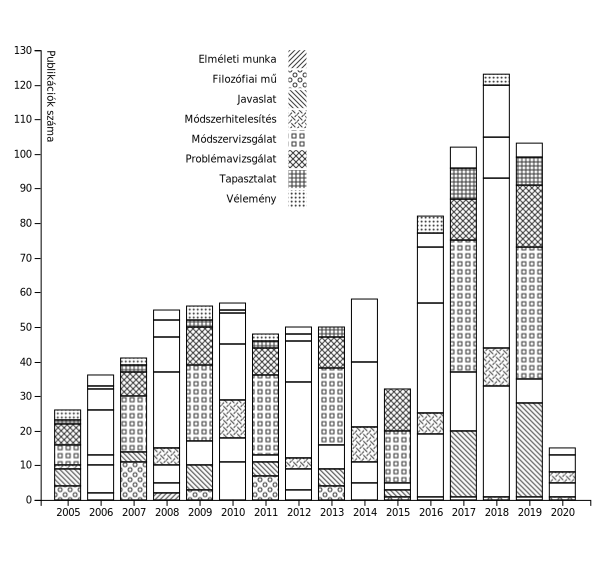
\includegraphics[width=0.5\textwidth,height=\textheight]{ábrák/SMS-Year-Type.svg}\label{fig:SMSYearType}}
\subfloat[Publikáció témája
szerint]{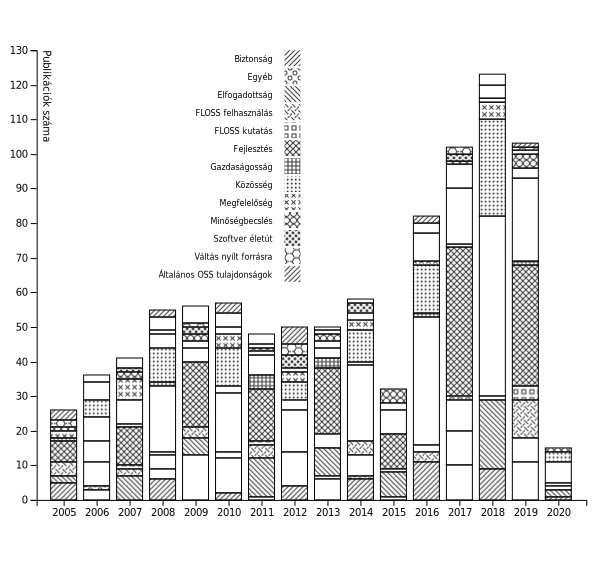
\includegraphics[width=0.5\textwidth,height=\textheight]{ábrák/SMS-Year-Topic.svg}\label{fig:SMSYearTopic}}

\caption{SMS osztályok kategóriái évenkénti bontásban (szerkesztette a
szerző).}

\label{fig:SMSByYear}

\end{figure}

Érdekes kérdés, hogy az egyes részterületeken mely kutatási módszerek az
irányadóak. A \ref{fig:SMSOSPMTH}. ábra bemutatja, hogy mely FLOSS
kategóriában hány publikáció alkalmazott egy bizonyos kutatási módszert.
Mint az korábban kiderült, az uralkodó kutatási módszerek az
esettanulmány a felmérés és az adatelemzés, de az eloszlásuk nem
teljesen azonos a FLOSS minden területén. A tudati dimenzió és
felhasználási kérdéseket elsősorban kérdőíves módszerrel igyekeznek
meghatározni -- mint az várható volt -- ezen a területen az
esettanulmányok és adatelemzések száma alacsonyabb, minden más módszer
elenyésző. A metaadatok területén -- tekintettel a nagy mennyiségű,
könnyen feldolgozható adatra -- az uralkodó módszer az adatelemzés,
ugyanakkor némiképp meglepő módon a kérdőíves módszereket itt is
előszeretettel alkalmazzák. Összességében elmondható, hogy az elemzett
publikációk jelentős része -- közel egynegyede -- tartalmaz valamilyen
fejlesztéssel kapcsolatos adatelemzést.

A kutatás szempontjából legnagyobb fontossággal bíró terület a
biztonság, amelynek módszereit külön vizsgáltam (\ref{fig:SMSSECMTH}.
ábra). Az alkalmazott módszerek eloszlását tekintve itt sem
tapasztalható jelentős eltérés, esettanulmányok, adatelemzések és
felmérések adják a publikációk nagy részét. Érdekes megfigyelni, hogy
bizonyos módszerek, például a modellanalízis szinte teljesen hiányoznak
ezen a területen. Közvetlen tapasztalatszerzésből, terepmunkából
származó eredményeket csak a szoftverminőség-vizsgálat, beszállítói lánc
elemzése és a sérülékenység-elemzés területén találunk, igaz ezeken a
területeken a minták száma túl alacsony ahhoz, hogy az eredményt
reprezentatívnak tekinthessük. Összességében elmondható, hogy a FLOSS
biztonsággal kapcsolatos kutatások döntő része biztonsági
sérülékenységekkel és szoftverbiztonsággal kapcsolatos esettanulmány és
adatelemzés.

Fontos kérdés, hogy az egyes részterületeken milyen típusú eredményekkel
találkozunk. A \ref{fig:SMSOSPCTR}. ábra az eredmények típusait mutatja
be FLOSS részterületek szerinti bontásban. Mint látható a tanulmányok
eredményeképpen első sorban metrikákat, modelleket és módszereket
kapunk, a folyamatleírások, taxonómiák és eszközök ismertetésének száma
elenyésző. Numerikus adatokat döntő részben a közösség, fejlesztés és
metaadatok kategóriában találhatunk, ami érthető, hiszen a nyílt forrás
jellegzetességének számító nyílt fejlesztési modellnek hála ezek a
numerikus adatok könnyen hozzáférhetők. A javasolt módszerek száma
viszonylag egyenletes, szinte minden kategóriában hasonló a forrásadatok
elérhetőségéhez viszonyítva, azaz a kutatók igyekeznek minden
részterületen módszereket javasolni. Mindez arra enged következtetni,
hogy a részterületek fontosságát a kutatók ismerik, de megfelelő
minőségű háttéradatok híján jóval kevesebb megalapozott tudományos
eredményt lehet ezeken a területeken felmutatni. Összességében
elmondható, hogy az eredmények döntő része a fejlesztés, közösség,
módszertan és felhasználás területen előállított metrika, modell és
módszertan.

A \ref{fig:SMSTYPSEC}. ábrán látható milyen típusú kutatások célozzák az
egyes biztonsági területeket. Szembeötlő, hogy a biztonság témáját
feldolgozó publikációk jelentős részét a szoftverminőség vizsgálat
területén már alkalmazott megoldások értékelése adja. Viszonylag
jelentős az ugyanezen területen végzett probléma és validációs
vizsgálatok, megoldási javaslatok száma, illetve a sérülékenységek
területén alkalmazott gyakorlati módszerek vizsgálata. Ugyanakkor
feltűnő, hogy sok a ``fehér folt'', azaz bizonyos biztonsági területeken
egyes módszerek teljesen hiányoznak. Nagyon kevés publikáció foglalkozik
a konfiguráció menedzsment és a tesztelés területével. A kockázatelemzés
területén, más kategóriáktól eltérően, a problémák vizsgálata és a
javasolt megoldások az uralkodók a módszervizsgálat túlsúlya itt nem
figyelhető meg.

\begin{figure}
\centering

\subfloat[FLOSS sajátosság szerint alkalmazott
módszertan]{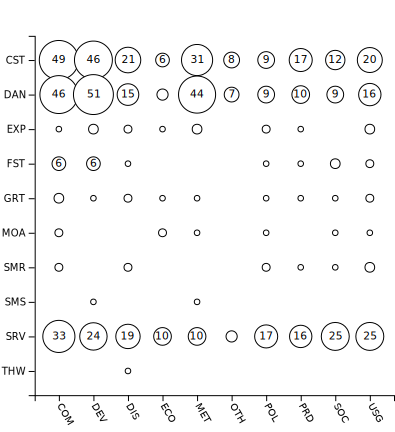
\includegraphics[width=0.5\textwidth,height=\textheight]{ábrák/SMS-OSP-MTH.svg}\label{fig:SMSOSPMTH}}
\subfloat[Biztonsági területenként alkalmazott
módszertan]{\includegraphics[width=0.5\textwidth,height=\textheight]{ábrák/SMS-SEC-MTH.svg}\label{fig:SMSSECMTH}}

\subfloat[FLOSS kategóriánként jellemző
eredményfajták]{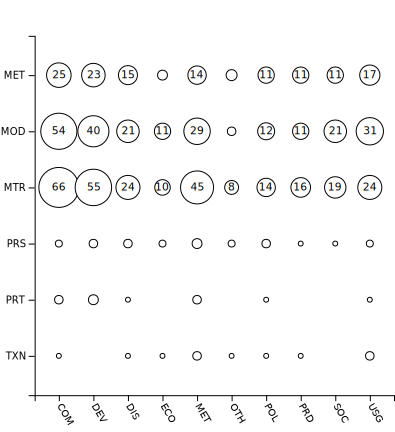
\includegraphics[width=0.5\textwidth,height=\textheight]{ábrák/SMS-OSP-CTR.svg}\label{fig:SMSOSPCTR}}
\subfloat[Publikáció típusok biztonsági
területenként]{\includegraphics[width=0.5\textwidth,height=\textheight]{ábrák/SMS-SEC-Type.svg}\label{fig:SMSTYPSEC}}

\caption{Publikációk száma az osztályok kategóriái szerint
(szerkesztette a szerző).}

\label{fig:SMSCategs}

\end{figure}

\hypertarget{sec:FSK}{%
\chapter{Függelék: FLOSS sajátosság kategóriák}\label{sec:FSK}}

\begin{longtable}[]{@{}ll@{}}
\caption{FLOSS sajátosság kategóriák}\tabularnewline
\toprule
kód & leírás\tabularnewline
\midrule
\endfirsthead
\toprule
kód & leírás\tabularnewline
\midrule
\endhead
FS-M & Fejlesztési metaadatok elérhetősége\tabularnewline
FS-F & Fejlesztési módszertan\tabularnewline
FS-G & Gazdasági és társadalmi hatás\tabularnewline
FS-K & Közösség (szubkultúra)\tabularnewline
FS-SZ & Szabályozás (compliance)\tabularnewline
FS-T & Terjesztés\tabularnewline
FS-J & Terméktulajdonságok\tabularnewline
\bottomrule
\end{longtable}

\begin{longtable}[]{@{}ll@{}}
\caption{FLOSS sajátosság alkategóriák}\tabularnewline
\toprule
kód & leírás\tabularnewline
\midrule
\endfirsthead
\toprule
kód & leírás\tabularnewline
\midrule
\endhead
FS-F-E & Egyedi fejlesztői eszközök\tabularnewline
FS-F-K & Eltérő követelmények\tabularnewline
FS-F-M & Minőségbiztosítási módszertan\tabularnewline
FS-F-P & Programtervezési metodika\tabularnewline
FS-F-T & Tesztelés\tabularnewline
FS-F-V & Kivitelezés és végrehajtás\tabularnewline
FS-G-G & Gazdasági hatás\tabularnewline
FS-G-T & Társadalmi hatás\tabularnewline
FS-H-F & Jellemző felhasználói tábor\tabularnewline
FS-H-I & Fejlesztés, integráció\tabularnewline
FS-H-M & Migráció\tabularnewline
FS-H-M & Választék, egyedi minősítés\tabularnewline
FS-H-P & Jellemző piaci szegmensek\tabularnewline
FS-H-T & Gyártófüggetlenség\tabularnewline
FS-H-T & Testreszabhatóság\tabularnewline
FS-J-Á & Átláthatóság, forráskód elérhetősége\tabularnewline
FS-J-D & Hiányos dokumentáció\tabularnewline
FS-J-H & Használhatóság, hordozhatóság\tabularnewline
FS-J-K & Kompatibilitás, szabványkövetés\tabularnewline
FS-J-M & Kódminőség, alacsony hibaszám\tabularnewline
FS-K-R & Résztvevők a közösségben\tabularnewline
FS-K-Sz & Szervezeti felépítés\tabularnewline
FS-M-A & Architektúra és API dokumentáció\tabularnewline
FS-M-F & Forrás publikus elérhetősége\tabularnewline
FS-M-H & Hibajegyek elérhetősége\tabularnewline
FS-M-K & Fejlesztői kommunikáció elérhetősége\tabularnewline
FS-SZ-B & Belső szabályozás\tabularnewline
FS-SZ-K & Kormányzati szabályozás\tabularnewline
FS-SZ-L & Összetett licencelés\tabularnewline
FS-SZ-M & Jog a módosításra\tabularnewline
FS-SZ-T & Tanúsítványok hiánya\tabularnewline
FS-T-E & Elérhetőség\tabularnewline
FS-T-K & Kiadási gyakoriság\tabularnewline
FS-T-L & Marketing és lobbierő hiánya\tabularnewline
FS-T-M & Terjesztés módja\tabularnewline
FS-T-T & Támogatás, support\tabularnewline
\bottomrule
\end{longtable}

\hypertarget{suxe9ruxfcluxe9kenysuxe9gek-uxe9s-javaslatok-kuxf3dtuxe1bluxe1zatai}{%
\section{Sérülékenységek és javaslatok
kódtáblázatai}\label{suxe9ruxfcluxe9kenysuxe9gek-uxe9s-javaslatok-kuxf3dtuxe1bluxe1zatai}}

\begin{longtable}[]{@{}rcl@{}}
\caption{Azonosított sérülékenységek}\tabularnewline
\toprule
\begin{minipage}[b]{0.04\columnwidth}\raggedleft
kód\strut
\end{minipage} & \begin{minipage}[b]{0.04\columnwidth}\centering
szint\strut
\end{minipage} & \begin{minipage}[b]{0.83\columnwidth}\raggedright
leírás\strut
\end{minipage}\tabularnewline
\midrule
\endfirsthead
\toprule
\begin{minipage}[b]{0.04\columnwidth}\raggedleft
kód\strut
\end{minipage} & \begin{minipage}[b]{0.04\columnwidth}\centering
szint\strut
\end{minipage} & \begin{minipage}[b]{0.83\columnwidth}\raggedright
leírás\strut
\end{minipage}\tabularnewline
\midrule
\endhead
\begin{minipage}[t]{0.04\columnwidth}\raggedleft
SF01\strut
\end{minipage} & \begin{minipage}[t]{0.04\columnwidth}\centering
1\strut
\end{minipage} & \begin{minipage}[t]{0.83\columnwidth}\raggedright
Nincs formális tesztelés, ami megnehezíti a minőség-ellenőrzést.\strut
\end{minipage}\tabularnewline
\begin{minipage}[t]{0.04\columnwidth}\raggedleft
SF02\strut
\end{minipage} & \begin{minipage}[t]{0.04\columnwidth}\centering
1\strut
\end{minipage} & \begin{minipage}[t]{0.83\columnwidth}\raggedright
Nem piac vezéreltek a követelmények, a biztonság nem feltétlen szempont,
amire nincs ráhatásunk.\strut
\end{minipage}\tabularnewline
\begin{minipage}[t]{0.04\columnwidth}\raggedleft
SF03\strut
\end{minipage} & \begin{minipage}[t]{0.04\columnwidth}\centering
1\strut
\end{minipage} & \begin{minipage}[t]{0.83\columnwidth}\raggedright
Nincs formális biztonsági tervezés az informális követelményeket nehéz
minősíteni.\strut
\end{minipage}\tabularnewline
\begin{minipage}[t]{0.04\columnwidth}\raggedleft
SF04\strut
\end{minipage} & \begin{minipage}[t]{0.04\columnwidth}\centering
3\strut
\end{minipage} & \begin{minipage}[t]{0.83\columnwidth}\raggedright
A kódbázisba sérülékenységet vezetnek be, ami az upstream változaton
keresztül eléri a szervezet kódbázisát.\strut
\end{minipage}\tabularnewline
\begin{minipage}[t]{0.04\columnwidth}\raggedleft
SF05\strut
\end{minipage} & \begin{minipage}[t]{0.04\columnwidth}\centering
1\strut
\end{minipage} & \begin{minipage}[t]{0.83\columnwidth}\raggedright
Hagyományos minőségbiztosítási elveknek nem felel meg, emiatt nehéz
összehasonlítani, értékelni.\strut
\end{minipage}\tabularnewline
\begin{minipage}[t]{0.04\columnwidth}\raggedleft
SF06\strut
\end{minipage} & \begin{minipage}[t]{0.04\columnwidth}\centering
1\strut
\end{minipage} & \begin{minipage}[t]{0.83\columnwidth}\raggedright
A beszállító vagy közösség nem monitorozza saját komponens projektjeit.
Az azokban bevezetett sérülékenység a terméken keresztül a szervezethez
is eljut.\strut
\end{minipage}\tabularnewline
\begin{minipage}[t]{0.04\columnwidth}\raggedleft
SF07\strut
\end{minipage} & \begin{minipage}[t]{0.04\columnwidth}\centering
3\strut
\end{minipage} & \begin{minipage}[t]{0.83\columnwidth}\raggedright
A szervezet forkolja az eredeti kódbázist, de nincs erőforrása
karbantartani azt.\strut
\end{minipage}\tabularnewline
\begin{minipage}[t]{0.04\columnwidth}\raggedleft
SF10\strut
\end{minipage} & \begin{minipage}[t]{0.04\columnwidth}\centering
3\strut
\end{minipage} & \begin{minipage}[t]{0.83\columnwidth}\raggedright
A komponensek közötti szoros függőségek miatt a komponens frissítése
számos részkomponens frissítését vonja maga után, ami ütközéshez és
hibákhoz vezethet.\strut
\end{minipage}\tabularnewline
\begin{minipage}[t]{0.04\columnwidth}\raggedleft
SF11\strut
\end{minipage} & \begin{minipage}[t]{0.04\columnwidth}\centering
3\strut
\end{minipage} & \begin{minipage}[t]{0.83\columnwidth}\raggedright
A kompatibilitás érdekében helyileg módosított komponens sérülékenységet
vezet be.\strut
\end{minipage}\tabularnewline
\begin{minipage}[t]{0.04\columnwidth}\raggedleft
SF12\strut
\end{minipage} & \begin{minipage}[t]{0.04\columnwidth}\centering
4\strut
\end{minipage} & \begin{minipage}[t]{0.83\columnwidth}\raggedright
A fejlesztőtábor kicsiny mérete lassítja vagy ellehetetleníti a
hozzájárulásaink időben történő integrálását.\strut
\end{minipage}\tabularnewline
\begin{minipage}[t]{0.04\columnwidth}\raggedleft
SF13\strut
\end{minipage} & \begin{minipage}[t]{0.04\columnwidth}\centering
2\strut
\end{minipage} & \begin{minipage}[t]{0.83\columnwidth}\raggedright
A fejlesztői vagy tesztelés alatti állapot használata növeli a
sérülékenységek esélyét\strut
\end{minipage}\tabularnewline
\begin{minipage}[t]{0.04\columnwidth}\raggedleft
SF14\strut
\end{minipage} & \begin{minipage}[t]{0.04\columnwidth}\centering
3\strut
\end{minipage} & \begin{minipage}[t]{0.83\columnwidth}\raggedright
A szervezet fejlesztőeszközei nem kompatibilisek a projektben
használtakkal, ami lassítja az együttműködést.\strut
\end{minipage}\tabularnewline
\begin{minipage}[t]{0.04\columnwidth}\raggedleft
SG01\strut
\end{minipage} & \begin{minipage}[t]{0.04\columnwidth}\centering
1\strut
\end{minipage} & \begin{minipage}[t]{0.83\columnwidth}\raggedright
Rejtett FLOSS használat miatt rosszul mérik fel a kockázatokat és nem
alkalmazzák a szükséges védelmi eljárásokat.\strut
\end{minipage}\tabularnewline
\begin{minipage}[t]{0.04\columnwidth}\raggedleft
SH01\strut
\end{minipage} & \begin{minipage}[t]{0.04\columnwidth}\centering
1\strut
\end{minipage} & \begin{minipage}[t]{0.83\columnwidth}\raggedright
A szervezet nem megfelelő minősítő rendszert alkalmaz a FLOSS termék
minősítésére.\strut
\end{minipage}\tabularnewline
\begin{minipage}[t]{0.04\columnwidth}\raggedleft
SH02\strut
\end{minipage} & \begin{minipage}[t]{0.04\columnwidth}\centering
1\strut
\end{minipage} & \begin{minipage}[t]{0.83\columnwidth}\raggedright
Megfelelő változat kiválasztása nehéz és időigényes. Emiatt
előfordulhat, hogy nem a megfelelő változat kerül alkalmazásra.\strut
\end{minipage}\tabularnewline
\begin{minipage}[t]{0.04\columnwidth}\raggedleft
SH03\strut
\end{minipage} & \begin{minipage}[t]{0.04\columnwidth}\centering
2\strut
\end{minipage} & \begin{minipage}[t]{0.83\columnwidth}\raggedright
A kontroll nélküli (esetleg rejtett) integráció a hibás komponensek
révén sérülékenységek akaratlan beépítéséhez vezet.\strut
\end{minipage}\tabularnewline
\begin{minipage}[t]{0.04\columnwidth}\raggedleft
SH04\strut
\end{minipage} & \begin{minipage}[t]{0.04\columnwidth}\centering
1\strut
\end{minipage} & \begin{minipage}[t]{0.83\columnwidth}\raggedright
A FLOSS komponensek minősítésére nem alkalmas a COTS esetén megszokott
módszertan.\strut
\end{minipage}\tabularnewline
\begin{minipage}[t]{0.04\columnwidth}\raggedleft
SH05\strut
\end{minipage} & \begin{minipage}[t]{0.04\columnwidth}\centering
2\strut
\end{minipage} & \begin{minipage}[t]{0.83\columnwidth}\raggedright
Az integrátor nem ismeri megfelelő mélységben az integrálandó komponenst
így hibákat vezet be az integráció során.\strut
\end{minipage}\tabularnewline
\begin{minipage}[t]{0.04\columnwidth}\raggedleft
SH06\strut
\end{minipage} & \begin{minipage}[t]{0.04\columnwidth}\centering
3\strut
\end{minipage} & \begin{minipage}[t]{0.83\columnwidth}\raggedright
Az integrált komponensen végzett módosítások összeütközésbe kerülnek az
eredeti kódbázissal, ami a frissítések során hibákhoz vagy
sérülékenységhez vezethet.\strut
\end{minipage}\tabularnewline
\begin{minipage}[t]{0.04\columnwidth}\raggedleft
SH07\strut
\end{minipage} & \begin{minipage}[t]{0.04\columnwidth}\centering
4\strut
\end{minipage} & \begin{minipage}[t]{0.83\columnwidth}\raggedright
A szükséges módosításokat nem sikerül visszavezetni, a közösség
elutasítja így a kódbázis ütközéseit folyamatosan figyelni kell, ami
időigényes és hibalehetőségekkel terhelt.\strut
\end{minipage}\tabularnewline
\begin{minipage}[t]{0.04\columnwidth}\raggedleft
SH08\strut
\end{minipage} & \begin{minipage}[t]{0.04\columnwidth}\centering
1\strut
\end{minipage} & \begin{minipage}[t]{0.83\columnwidth}\raggedright
Az integrált komponens összetett függőségein keresztül hibás (és
ellenőrizetlen) alkomponensek szivároghatnak a fejlesztésbe.\strut
\end{minipage}\tabularnewline
\begin{minipage}[t]{0.04\columnwidth}\raggedleft
SH09\strut
\end{minipage} & \begin{minipage}[t]{0.04\columnwidth}\centering
4\strut
\end{minipage} & \begin{minipage}[t]{0.83\columnwidth}\raggedright
A módosítások visszavezetése során érzékeny információ szivárog ki az
upstream projektbe.\strut
\end{minipage}\tabularnewline
\begin{minipage}[t]{0.04\columnwidth}\raggedleft
SH10\strut
\end{minipage} & \begin{minipage}[t]{0.04\columnwidth}\centering
1\strut
\end{minipage} & \begin{minipage}[t]{0.83\columnwidth}\raggedright
Kompatibilitási problémák miatt a szervezet által alkalmazott
felügyeleti rendszer nem támogatja a FLOSS változatot.\strut
\end{minipage}\tabularnewline
\begin{minipage}[t]{0.04\columnwidth}\raggedleft
SH11\strut
\end{minipage} & \begin{minipage}[t]{0.04\columnwidth}\centering
1\strut
\end{minipage} & \begin{minipage}[t]{0.83\columnwidth}\raggedright
A szükséges adatmigrációt követően a korábbi mentések helyreállítása
nehézzé vagy lehetetlenné válik, veszélyeztetve a rendelkezésre
állást.\strut
\end{minipage}\tabularnewline
\begin{minipage}[t]{0.04\columnwidth}\raggedleft
SJ01\strut
\end{minipage} & \begin{minipage}[t]{0.04\columnwidth}\centering
2\strut
\end{minipage} & \begin{minipage}[t]{0.83\columnwidth}\raggedright
A dokumentáció és a tényleges képességek és szükséges konfiguráció közt
jelentős eltérés lehet, ami biztonsági problémákhoz vezethet.\strut
\end{minipage}\tabularnewline
\begin{minipage}[t]{0.04\columnwidth}\raggedleft
SJ02\strut
\end{minipage} & \begin{minipage}[t]{0.04\columnwidth}\centering
2\strut
\end{minipage} & \begin{minipage}[t]{0.83\columnwidth}\raggedright
Megfelelő alapértelmezett beállítások híján a felhasználó
(türelmetlenségből vagy figyelmetlenségből) hibás beállításokat
alkalmazhat.\strut
\end{minipage}\tabularnewline
\begin{minipage}[t]{0.04\columnwidth}\raggedleft
SJ03\strut
\end{minipage} & \begin{minipage}[t]{0.04\columnwidth}\centering
1\strut
\end{minipage} & \begin{minipage}[t]{0.83\columnwidth}\raggedright
A meglévő zárt rendszerekkel való inkompatibilitás.\strut
\end{minipage}\tabularnewline
\begin{minipage}[t]{0.04\columnwidth}\raggedleft
SK01\strut
\end{minipage} & \begin{minipage}[t]{0.04\columnwidth}\centering
1\strut
\end{minipage} & \begin{minipage}[t]{0.83\columnwidth}\raggedright
A fejlesztők és a hibabejelentők közötti kommunikáció nem
megfelelő.\strut
\end{minipage}\tabularnewline
\begin{minipage}[t]{0.04\columnwidth}\raggedleft
SK02\strut
\end{minipage} & \begin{minipage}[t]{0.04\columnwidth}\centering
1\strut
\end{minipage} & \begin{minipage}[t]{0.83\columnwidth}\raggedright
Az alkotók nem mindig beazonosíthatók. Nehéz megállapítani, hogy több
részmunkát ugyanaz a személy végezte-e el vagy sem.\strut
\end{minipage}\tabularnewline
\begin{minipage}[t]{0.04\columnwidth}\raggedleft
SK03\strut
\end{minipage} & \begin{minipage}[t]{0.04\columnwidth}\centering
1\strut
\end{minipage} & \begin{minipage}[t]{0.83\columnwidth}\raggedright
Az erős cégirányítás miatt a fejlesztők elhagyják a projektet,
veszélyeztetve a támogatást\strut
\end{minipage}\tabularnewline
\begin{minipage}[t]{0.04\columnwidth}\raggedleft
SK04\strut
\end{minipage} & \begin{minipage}[t]{0.04\columnwidth}\centering
4\strut
\end{minipage} & \begin{minipage}[t]{0.83\columnwidth}\raggedright
Rossz vagy az elvárásoknak nem megfelelő kód küldése a bizalom, ezáltal
az OSSD feletti irányítás elvesztését okozza.\strut
\end{minipage}\tabularnewline
\begin{minipage}[t]{0.04\columnwidth}\raggedleft
SK05\strut
\end{minipage} & \begin{minipage}[t]{0.04\columnwidth}\centering
1\strut
\end{minipage} & \begin{minipage}[t]{0.83\columnwidth}\raggedright
Az OSSD vezető szereplője távozik (cég akvizíciója, fejlesztő kilépése),
a támogatás folytonossága veszélybe kerül.\strut
\end{minipage}\tabularnewline
\begin{minipage}[t]{0.04\columnwidth}\raggedleft
SK06\strut
\end{minipage} & \begin{minipage}[t]{0.04\columnwidth}\centering
4\strut
\end{minipage} & \begin{minipage}[t]{0.83\columnwidth}\raggedright
A delegált fejlesztők nyílt kommunikációja érzékeny adatokat tesz
publikussá.\strut
\end{minipage}\tabularnewline
\begin{minipage}[t]{0.04\columnwidth}\raggedleft
SM01\strut
\end{minipage} & \begin{minipage}[t]{0.04\columnwidth}\centering
2\strut
\end{minipage} & \begin{minipage}[t]{0.83\columnwidth}\raggedright
A hibajegy válasz nélkül maradhat.\strut
\end{minipage}\tabularnewline
\begin{minipage}[t]{0.04\columnwidth}\raggedleft
SM02\strut
\end{minipage} & \begin{minipage}[t]{0.04\columnwidth}\centering
2\strut
\end{minipage} & \begin{minipage}[t]{0.83\columnwidth}\raggedright
A hiba javításának ellenőrzése késhet.\strut
\end{minipage}\tabularnewline
\begin{minipage}[t]{0.04\columnwidth}\raggedleft
SM03\strut
\end{minipage} & \begin{minipage}[t]{0.04\columnwidth}\centering
2\strut
\end{minipage} & \begin{minipage}[t]{0.83\columnwidth}\raggedright
A hiba nem reprodukálható ezért figyelmen kívül hagyják\strut
\end{minipage}\tabularnewline
\begin{minipage}[t]{0.04\columnwidth}\raggedleft
SM04\strut
\end{minipage} & \begin{minipage}[t]{0.04\columnwidth}\centering
1\strut
\end{minipage} & \begin{minipage}[t]{0.83\columnwidth}\raggedright
A forrástároló, a publikus hibajegyek és a hozzá tartozó foltok
folyamatos analízisével a támadó sérülékenységeket fedezhet fel és
használhat ki még azok javítása előtt.\strut
\end{minipage}\tabularnewline
\begin{minipage}[t]{0.04\columnwidth}\raggedleft
SM05\strut
\end{minipage} & \begin{minipage}[t]{0.04\columnwidth}\centering
2\strut
\end{minipage} & \begin{minipage}[t]{0.83\columnwidth}\raggedright
A hibajegy hibakeresési csatolmányaként érzékeny információ kerül a
publikus hibakereső rendszerre.\strut
\end{minipage}\tabularnewline
\begin{minipage}[t]{0.04\columnwidth}\raggedleft
SM06\strut
\end{minipage} & \begin{minipage}[t]{0.04\columnwidth}\centering
1\strut
\end{minipage} & \begin{minipage}[t]{0.83\columnwidth}\raggedright
A nyilvános fejlesztői dokumentáció tervezési hiányosságokat tárhat
fel.\strut
\end{minipage}\tabularnewline
\begin{minipage}[t]{0.04\columnwidth}\raggedleft
SM07\strut
\end{minipage} & \begin{minipage}[t]{0.04\columnwidth}\centering
1\strut
\end{minipage} & \begin{minipage}[t]{0.83\columnwidth}\raggedright
A fejlesztői kommunikáció elemzésével a támadó még javítás előtt
tudomást szerezhet a sérülékenységről.\strut
\end{minipage}\tabularnewline
\begin{minipage}[t]{0.04\columnwidth}\raggedleft
SM08\strut
\end{minipage} & \begin{minipage}[t]{0.04\columnwidth}\centering
1\strut
\end{minipage} & \begin{minipage}[t]{0.83\columnwidth}\raggedright
A támadó automatikus vagy manuális kódanalízise sérülékenységet fed
fel.\strut
\end{minipage}\tabularnewline
\begin{minipage}[t]{0.04\columnwidth}\raggedleft
SM09\strut
\end{minipage} & \begin{minipage}[t]{0.04\columnwidth}\centering
1\strut
\end{minipage} & \begin{minipage}[t]{0.83\columnwidth}\raggedright
A támadó fél a forráskódban rejtett sérülékenységet helyez el.\strut
\end{minipage}\tabularnewline
\begin{minipage}[t]{0.04\columnwidth}\raggedleft
SM10\strut
\end{minipage} & \begin{minipage}[t]{0.04\columnwidth}\centering
4\strut
\end{minipage} & \begin{minipage}[t]{0.83\columnwidth}\raggedright
Nem világos hogyan kerül összhangba a forráskódban tárolt személyi
adatok kérdése az adatvédelmi szabályozással (pl. GDPR).\strut
\end{minipage}\tabularnewline
\begin{minipage}[t]{0.04\columnwidth}\raggedleft
SM11\strut
\end{minipage} & \begin{minipage}[t]{0.04\columnwidth}\centering
1\strut
\end{minipage} & \begin{minipage}[t]{0.83\columnwidth}\raggedright
Az architektúra dokumentáció sokszor hiányos, így a tervezési hibákból
adódó sérülékenységek nem nyilvánvalóak.\strut
\end{minipage}\tabularnewline
\begin{minipage}[t]{0.04\columnwidth}\raggedleft
SS01\strut
\end{minipage} & \begin{minipage}[t]{0.04\columnwidth}\centering
2\strut
\end{minipage} & \begin{minipage}[t]{0.83\columnwidth}\raggedright
A megfelelő belső FLOSS szabályozás hiánya, átláthatatlan FLOSS
felhasználáshoz vezet, a problémákat nem lehet megfelelően
kezelni.\strut
\end{minipage}\tabularnewline
\begin{minipage}[t]{0.04\columnwidth}\raggedleft
SS02\strut
\end{minipage} & \begin{minipage}[t]{0.04\columnwidth}\centering
2\strut
\end{minipage} & \begin{minipage}[t]{0.83\columnwidth}\raggedright
FLOSS komponens-felhasználás esetén az összetett és rejtett licencelés a
szervezet tudta nélkül kompromittálhatja a jogszabályi megfelelést, ami
kikényszerített határidős módosításokhoz vezet, veszélyeztetve a
rendszer rendelkezésre állását és integritását.\strut
\end{minipage}\tabularnewline
\begin{minipage}[t]{0.04\columnwidth}\raggedleft
SS03\strut
\end{minipage} & \begin{minipage}[t]{0.04\columnwidth}\centering
2\strut
\end{minipage} & \begin{minipage}[t]{0.83\columnwidth}\raggedright
A termék összetett függőségeiben ellentmondásos licencek találhatók vagy
a licencelés megváltozik ami ellentmondáshoz vezet.\strut
\end{minipage}\tabularnewline
\begin{minipage}[t]{0.04\columnwidth}\raggedleft
SS04\strut
\end{minipage} & \begin{minipage}[t]{0.04\columnwidth}\centering
2\strut
\end{minipage} & \begin{minipage}[t]{0.83\columnwidth}\raggedright
FLOSS projektek ritkán szereznek tanúsítást. Következésképpen nem
alkalmazhatók olyan területeken ahol a tanúsítvány megléte
előkövetelmény.\strut
\end{minipage}\tabularnewline
\begin{minipage}[t]{0.04\columnwidth}\raggedleft
SS05\strut
\end{minipage} & \begin{minipage}[t]{0.04\columnwidth}\centering
1\strut
\end{minipage} & \begin{minipage}[t]{0.83\columnwidth}\raggedright
GPL licencű alkalmazások nem integrálhatják a szabadalomhoz kötött
biztonsági megoldásokat\strut
\end{minipage}\tabularnewline
\begin{minipage}[t]{0.04\columnwidth}\raggedleft
ST01\strut
\end{minipage} & \begin{minipage}[t]{0.04\columnwidth}\centering
1\strut
\end{minipage} & \begin{minipage}[t]{0.83\columnwidth}\raggedright
A gyors kiadási sűrűség és munkaigényes frissítés miatt a biztonsági
javításokat nem vezetik át a downstream termékbe\strut
\end{minipage}\tabularnewline
\begin{minipage}[t]{0.04\columnwidth}\raggedleft
ST02\strut
\end{minipage} & \begin{minipage}[t]{0.04\columnwidth}\centering
2\strut
\end{minipage} & \begin{minipage}[t]{0.83\columnwidth}\raggedright
Nincs szerződésben biztosított időkorlát a javításra, a javítás
késhet.\strut
\end{minipage}\tabularnewline
\begin{minipage}[t]{0.04\columnwidth}\raggedleft
ST03\strut
\end{minipage} & \begin{minipage}[t]{0.04\columnwidth}\centering
2\strut
\end{minipage} & \begin{minipage}[t]{0.83\columnwidth}\raggedright
Az udvariatlanul kért hibajavítást nem javítják megfelelő
sebességgel.\strut
\end{minipage}\tabularnewline
\begin{minipage}[t]{0.04\columnwidth}\raggedleft
ST04\strut
\end{minipage} & \begin{minipage}[t]{0.04\columnwidth}\centering
2\strut
\end{minipage} & \begin{minipage}[t]{0.83\columnwidth}\raggedright
Kiadás csúszása miatt a fejlesztői verziót kezdik el használni.\strut
\end{minipage}\tabularnewline
\begin{minipage}[t]{0.04\columnwidth}\raggedleft
ST05\strut
\end{minipage} & \begin{minipage}[t]{0.04\columnwidth}\centering
2\strut
\end{minipage} & \begin{minipage}[t]{0.83\columnwidth}\raggedright
A szervezet félkész terméket tölt le.\strut
\end{minipage}\tabularnewline
\begin{minipage}[t]{0.04\columnwidth}\raggedleft
ST06\strut
\end{minipage} & \begin{minipage}[t]{0.04\columnwidth}\centering
2\strut
\end{minipage} & \begin{minipage}[t]{0.83\columnwidth}\raggedright
Nincs szakemberképzés, előfordulhat, hogy a szervezet nem talál
megfelelő szakembert, nincs tanúsítás a szaktudásra.\strut
\end{minipage}\tabularnewline
\begin{minipage}[t]{0.04\columnwidth}\raggedleft
ST07\strut
\end{minipage} & \begin{minipage}[t]{0.04\columnwidth}\centering
2\strut
\end{minipage} & \begin{minipage}[t]{0.83\columnwidth}\raggedright
Nincs szervezett képzés, az autodidakta tanulás minősége nem garantál,
ami hibákhoz vezethet.\strut
\end{minipage}\tabularnewline
\begin{minipage}[t]{0.04\columnwidth}\raggedleft
ST08\strut
\end{minipage} & \begin{minipage}[t]{0.04\columnwidth}\centering
2\strut
\end{minipage} & \begin{minipage}[t]{0.83\columnwidth}\raggedright
A letöltött bináris változat nem a kiadott forrásból készült\strut
\end{minipage}\tabularnewline
\begin{minipage}[t]{0.04\columnwidth}\raggedleft
ST09\strut
\end{minipage} & \begin{minipage}[t]{0.04\columnwidth}\centering
2\strut
\end{minipage} & \begin{minipage}[t]{0.83\columnwidth}\raggedright
A letöltött bináris ellenőrzőösszegét vagy aláírását a felhasználó nem
ellenőrzi.\strut
\end{minipage}\tabularnewline
\begin{minipage}[t]{0.04\columnwidth}\raggedleft
ST10\strut
\end{minipage} & \begin{minipage}[t]{0.04\columnwidth}\centering
1\strut
\end{minipage} & \begin{minipage}[t]{0.83\columnwidth}\raggedright
A keresőmotor nem a megfelelő verziót vagy disztribútort hozza
fel.\strut
\end{minipage}\tabularnewline
\begin{minipage}[t]{0.04\columnwidth}\raggedleft
ST11\strut
\end{minipage} & \begin{minipage}[t]{0.04\columnwidth}\centering
2\strut
\end{minipage} & \begin{minipage}[t]{0.83\columnwidth}\raggedright
A felhasznált csomagkezelő rendszer (CPAN, hackage, deb) támadásával a
felhasznált komponens támadható.\strut
\end{minipage}\tabularnewline
\begin{minipage}[t]{0.04\columnwidth}\raggedleft
ST12\strut
\end{minipage} & \begin{minipage}[t]{0.04\columnwidth}\centering
1\strut
\end{minipage} & \begin{minipage}[t]{0.83\columnwidth}\raggedright
Fejlesztői kapcsolati információk hiányában a felfedett sérülékenységek
bejelentése nehézségekbe ütközik, nincs biztonsági kapcsolattartó
személy vagy fórum megjelölve.\strut
\end{minipage}\tabularnewline
\bottomrule
\end{longtable}

\begin{longtable}[]{@{}rcl@{}}
\caption{Azonosított javaslatok}\tabularnewline
\toprule
\begin{minipage}[b]{0.04\columnwidth}\raggedleft
kód\strut
\end{minipage} & \begin{minipage}[b]{0.04\columnwidth}\centering
szint\strut
\end{minipage} & \begin{minipage}[b]{0.83\columnwidth}\raggedright
leírás\strut
\end{minipage}\tabularnewline
\midrule
\endfirsthead
\toprule
\begin{minipage}[b]{0.04\columnwidth}\raggedleft
kód\strut
\end{minipage} & \begin{minipage}[b]{0.04\columnwidth}\centering
szint\strut
\end{minipage} & \begin{minipage}[b]{0.83\columnwidth}\raggedright
leírás\strut
\end{minipage}\tabularnewline
\midrule
\endhead
\begin{minipage}[t]{0.04\columnwidth}\raggedleft
JF01\strut
\end{minipage} & \begin{minipage}[t]{0.04\columnwidth}\centering
4\strut
\end{minipage} & \begin{minipage}[t]{0.83\columnwidth}\raggedright
A szervezet részt vesz a projekt fejlesztésében, így biztosítva a
számára kedvező célok elérését.\strut
\end{minipage}\tabularnewline
\begin{minipage}[t]{0.04\columnwidth}\raggedleft
JF02\strut
\end{minipage} & \begin{minipage}[t]{0.04\columnwidth}\centering
4\strut
\end{minipage} & \begin{minipage}[t]{0.83\columnwidth}\raggedright
A kód-hozzájárulásokat a projektre vonatkozó formai és minőségi
szabályok betartásával, lehetőleg egy ismert közösségi tag segítségével
kell bevezetni.\strut
\end{minipage}\tabularnewline
\begin{minipage}[t]{0.04\columnwidth}\raggedleft
JF03\strut
\end{minipage} & \begin{minipage}[t]{0.04\columnwidth}\centering
1\strut
\end{minipage} & \begin{minipage}[t]{0.83\columnwidth}\raggedright
Közvetlenül, kvantitatív módon ellenőrizhető a minőség szintje.\strut
\end{minipage}\tabularnewline
\begin{minipage}[t]{0.04\columnwidth}\raggedleft
JF04\strut
\end{minipage} & \begin{minipage}[t]{0.04\columnwidth}\centering
3\strut
\end{minipage} & \begin{minipage}[t]{0.83\columnwidth}\raggedright
Lehetőség van saját alternatív (forkolt) változat létrehozására.\strut
\end{minipage}\tabularnewline
\begin{minipage}[t]{0.04\columnwidth}\raggedleft
JF05\strut
\end{minipage} & \begin{minipage}[t]{0.04\columnwidth}\centering
2\strut
\end{minipage} & \begin{minipage}[t]{0.83\columnwidth}\raggedright
Egy adott állapot rögzítésével (snapshot) elkerülhető a folyamatos
változás okozta problémák egy része.\strut
\end{minipage}\tabularnewline
\begin{minipage}[t]{0.04\columnwidth}\raggedleft
JF06\strut
\end{minipage} & \begin{minipage}[t]{0.04\columnwidth}\centering
1\strut
\end{minipage} & \begin{minipage}[t]{0.83\columnwidth}\raggedright
Az átláthatóság lehetővé teszi az önbevallás alapú minősítést a
kódminőség és legjobb fejlesztési gyakorlat terén.\strut
\end{minipage}\tabularnewline
\begin{minipage}[t]{0.04\columnwidth}\raggedleft
JG01\strut
\end{minipage} & \begin{minipage}[t]{0.04\columnwidth}\centering
1\strut
\end{minipage} & \begin{minipage}[t]{0.83\columnwidth}\raggedright
A FLOSS állami vagy nemzetközi szinten kell támogatni, mert fellendülése
a munkaoptimalizáció révén növeli az információbiztonságot.\strut
\end{minipage}\tabularnewline
\begin{minipage}[t]{0.04\columnwidth}\raggedleft
JG02\strut
\end{minipage} & \begin{minipage}[t]{0.04\columnwidth}\centering
2\strut
\end{minipage} & \begin{minipage}[t]{0.83\columnwidth}\raggedright
A nyílt modell kockázatainak és lehetőségeinek oktatása szerepeljen a
megfelelő oktatási intézményekben.\strut
\end{minipage}\tabularnewline
\begin{minipage}[t]{0.04\columnwidth}\raggedleft
JG03\strut
\end{minipage} & \begin{minipage}[t]{0.04\columnwidth}\centering
3\strut
\end{minipage} & \begin{minipage}[t]{0.83\columnwidth}\raggedright
Országos vagy európai egységes forráskód kezelő rendszer kialakítása
szükséges.\strut
\end{minipage}\tabularnewline
\begin{minipage}[t]{0.04\columnwidth}\raggedleft
JH01\strut
\end{minipage} & \begin{minipage}[t]{0.04\columnwidth}\centering
1\strut
\end{minipage} & \begin{minipage}[t]{0.83\columnwidth}\raggedright
Formális tanúsítás híján a felhasznált komponensek kódját megbízhatósági
modellekkel kell vizsgálni (pl. CodeTrust).\strut
\end{minipage}\tabularnewline
\begin{minipage}[t]{0.04\columnwidth}\raggedleft
JH02\strut
\end{minipage} & \begin{minipage}[t]{0.04\columnwidth}\centering
3\strut
\end{minipage} & \begin{minipage}[t]{0.83\columnwidth}\raggedright
A kód szabad módosíthatósága miatt várakozás nélkül javíthatóak a
sérülékenységek, amennyiben a kód módosításához szükséges erőforrás és
szakismeret rendelkezésre áll.\strut
\end{minipage}\tabularnewline
\begin{minipage}[t]{0.04\columnwidth}\raggedleft
JH04\strut
\end{minipage} & \begin{minipage}[t]{0.04\columnwidth}\centering
2\strut
\end{minipage} & \begin{minipage}[t]{0.83\columnwidth}\raggedright
A felhasználandó FLOSS komponenseket erre szakosodott szakértők révén
szerezzük be.\strut
\end{minipage}\tabularnewline
\begin{minipage}[t]{0.04\columnwidth}\raggedleft
JH05\strut
\end{minipage} & \begin{minipage}[t]{0.04\columnwidth}\centering
1\strut
\end{minipage} & \begin{minipage}[t]{0.83\columnwidth}\raggedright
A FLOSS komponens kiválasztásának folyamatát és körülményeit
dokumentálni kell.\strut
\end{minipage}\tabularnewline
\begin{minipage}[t]{0.04\columnwidth}\raggedleft
JH06\strut
\end{minipage} & \begin{minipage}[t]{0.04\columnwidth}\centering
4\strut
\end{minipage} & \begin{minipage}[t]{0.83\columnwidth}\raggedright
A kód változásait lehetőség szerint vissza kell vezetni az eredeti
projektbe.\strut
\end{minipage}\tabularnewline
\begin{minipage}[t]{0.04\columnwidth}\raggedleft
JH07\strut
\end{minipage} & \begin{minipage}[t]{0.04\columnwidth}\centering
3\strut
\end{minipage} & \begin{minipage}[t]{0.83\columnwidth}\raggedright
A fejlesztést végző részlegnek legyen megfelelő verzió-követési
terve.\strut
\end{minipage}\tabularnewline
\begin{minipage}[t]{0.04\columnwidth}\raggedleft
JH08\strut
\end{minipage} & \begin{minipage}[t]{0.04\columnwidth}\centering
3\strut
\end{minipage} & \begin{minipage}[t]{0.83\columnwidth}\raggedright
A beszállító vagy a fejlesztést végző részleg alkalmazzon FLOSS
komponens kezelő keretrendszert.\strut
\end{minipage}\tabularnewline
\begin{minipage}[t]{0.04\columnwidth}\raggedleft
JH10\strut
\end{minipage} & \begin{minipage}[t]{0.04\columnwidth}\centering
4\strut
\end{minipage} & \begin{minipage}[t]{0.83\columnwidth}\raggedright
A forráskódban minden nem publikus információ világosan definiált
legyen. A változások visszavezetésekor automatizált rendszerrel meg kell
akadályozni a minősített információ kiszivárgását.\strut
\end{minipage}\tabularnewline
\begin{minipage}[t]{0.04\columnwidth}\raggedleft
JH11\strut
\end{minipage} & \begin{minipage}[t]{0.04\columnwidth}\centering
2\strut
\end{minipage} & \begin{minipage}[t]{0.83\columnwidth}\raggedright
Képzésekkel kell tudatosítani a komponens integrációval járó veszélyeket
és a biztonságos felhasználáshoz szükséges eljárásokat\strut
\end{minipage}\tabularnewline
\begin{minipage}[t]{0.04\columnwidth}\raggedleft
JJ01\strut
\end{minipage} & \begin{minipage}[t]{0.04\columnwidth}\centering
1\strut
\end{minipage} & \begin{minipage}[t]{0.83\columnwidth}\raggedright
Ki kell használni a nyílt forrás nyilvános adatait a termékminősítés
kalibrációja és validálása során.\strut
\end{minipage}\tabularnewline
\begin{minipage}[t]{0.04\columnwidth}\raggedleft
JJ02\strut
\end{minipage} & \begin{minipage}[t]{0.04\columnwidth}\centering
1\strut
\end{minipage} & \begin{minipage}[t]{0.83\columnwidth}\raggedright
A minősítés belsőleg is elvégezhető, bár rendkívül
erőforrásigényes.\strut
\end{minipage}\tabularnewline
\begin{minipage}[t]{0.04\columnwidth}\raggedleft
JJ03\strut
\end{minipage} & \begin{minipage}[t]{0.04\columnwidth}\centering
1\strut
\end{minipage} & \begin{minipage}[t]{0.83\columnwidth}\raggedright
Szükség esetén harmadik felet kell felkérni a biztonsági hiányosságok
feltárására és a komponens minősítésére.\strut
\end{minipage}\tabularnewline
\begin{minipage}[t]{0.04\columnwidth}\raggedleft
JK01\strut
\end{minipage} & \begin{minipage}[t]{0.04\columnwidth}\centering
4\strut
\end{minipage} & \begin{minipage}[t]{0.83\columnwidth}\raggedright
A közösségbe fejlesztőket kell delegálni akiknek lehetőség szerint
mentort kell keresni.\strut
\end{minipage}\tabularnewline
\begin{minipage}[t]{0.04\columnwidth}\raggedleft
JK02\strut
\end{minipage} & \begin{minipage}[t]{0.04\columnwidth}\centering
2\strut
\end{minipage} & \begin{minipage}[t]{0.83\columnwidth}\raggedright
A belső szerkezet elemezhető, meghatározhatók a kulcsszereplők. Az
adatok alapján kockázatelemzés végezhető.\strut
\end{minipage}\tabularnewline
\begin{minipage}[t]{0.04\columnwidth}\raggedleft
JK03\strut
\end{minipage} & \begin{minipage}[t]{0.04\columnwidth}\centering
2\strut
\end{minipage} & \begin{minipage}[t]{0.83\columnwidth}\raggedright
A digitális aláírásokat használó fejlesztők nyílt kulcsait (rendszerint
GPG) be kell szerezni, biztonságos adatbázisban kell tárolni,
hozzáférhetővé tenni és szükség esetén ellenőrizni.\strut
\end{minipage}\tabularnewline
\begin{minipage}[t]{0.04\columnwidth}\raggedleft
JK04\strut
\end{minipage} & \begin{minipage}[t]{0.04\columnwidth}\centering
2\strut
\end{minipage} & \begin{minipage}[t]{0.83\columnwidth}\raggedright
Folyamatosan monitorozni kell a közösséget.\strut
\end{minipage}\tabularnewline
\begin{minipage}[t]{0.04\columnwidth}\raggedleft
JK05\strut
\end{minipage} & \begin{minipage}[t]{0.04\columnwidth}\centering
2\strut
\end{minipage} & \begin{minipage}[t]{0.83\columnwidth}\raggedright
Megfelelő lobbierőt kell kiépíteni az érdekérvényesítő képesség
érdekében.\strut
\end{minipage}\tabularnewline
\begin{minipage}[t]{0.04\columnwidth}\raggedleft
JK06\strut
\end{minipage} & \begin{minipage}[t]{0.04\columnwidth}\centering
2\strut
\end{minipage} & \begin{minipage}[t]{0.83\columnwidth}\raggedright
Kapcsolatépítéssel és személyes találkozásokkal erősíthető a közösséggel
való együttműködés (pl.találkozók szervezése).\strut
\end{minipage}\tabularnewline
\begin{minipage}[t]{0.04\columnwidth}\raggedleft
JK07\strut
\end{minipage} & \begin{minipage}[t]{0.04\columnwidth}\centering
2\strut
\end{minipage} & \begin{minipage}[t]{0.83\columnwidth}\raggedright
A vezetőkben tudatosítani kell, hogy az OSSD fejlesztőit más módon kell
motiválni.\strut
\end{minipage}\tabularnewline
\begin{minipage}[t]{0.04\columnwidth}\raggedleft
JK08\strut
\end{minipage} & \begin{minipage}[t]{0.04\columnwidth}\centering
4\strut
\end{minipage} & \begin{minipage}[t]{0.83\columnwidth}\raggedright
Felelőst kell kijelölni (Gatekeeper) aki a közösséggel való
kapcsolattartást és az oda áramló információt ellenőrzi.\strut
\end{minipage}\tabularnewline
\begin{minipage}[t]{0.04\columnwidth}\raggedleft
JK09\strut
\end{minipage} & \begin{minipage}[t]{0.04\columnwidth}\centering
4\strut
\end{minipage} & \begin{minipage}[t]{0.83\columnwidth}\raggedright
A közösségbe delegált fejlesztők elkülönített kommunikációja előnytelen,
a közösségi csatornán folyó kommunikáció információtartalmára oda kell
figyelni.\strut
\end{minipage}\tabularnewline
\begin{minipage}[t]{0.04\columnwidth}\raggedleft
JM01\strut
\end{minipage} & \begin{minipage}[t]{0.04\columnwidth}\centering
1\strut
\end{minipage} & \begin{minipage}[t]{0.83\columnwidth}\raggedright
Automatizált módszerekkel elemezhetőek a hibajegyek adatai\strut
\end{minipage}\tabularnewline
\begin{minipage}[t]{0.04\columnwidth}\raggedleft
JM02\strut
\end{minipage} & \begin{minipage}[t]{0.04\columnwidth}\centering
2\strut
\end{minipage} & \begin{minipage}[t]{0.83\columnwidth}\raggedright
Be kell azonosítani azokat a fejlesztőket, akik hatékonyan javítják a
hibákat.\strut
\end{minipage}\tabularnewline
\begin{minipage}[t]{0.04\columnwidth}\raggedleft
JM03\strut
\end{minipage} & \begin{minipage}[t]{0.04\columnwidth}\centering
2\strut
\end{minipage} & \begin{minipage}[t]{0.83\columnwidth}\raggedright
Be kell azonosítani és követni azokat a hibakeresőket, akik valóban
értékes hibajegyeket vesznek fel.\strut
\end{minipage}\tabularnewline
\begin{minipage}[t]{0.04\columnwidth}\raggedleft
JM04\strut
\end{minipage} & \begin{minipage}[t]{0.04\columnwidth}\centering
2\strut
\end{minipage} & \begin{minipage}[t]{0.83\columnwidth}\raggedright
A hibakezelésben és fejlesztői kommunikációban aktív módon részt kell
venni, az információáramlás gyorsítása végett.\strut
\end{minipage}\tabularnewline
\begin{minipage}[t]{0.04\columnwidth}\raggedleft
JM05\strut
\end{minipage} & \begin{minipage}[t]{0.04\columnwidth}\centering
1\strut
\end{minipage} & \begin{minipage}[t]{0.83\columnwidth}\raggedright
Kódminőség vizsgálati módszerekkel elemezni lehet az elérhető
forráskódot, ami szolgáltatásként is igénybe vehető.\strut
\end{minipage}\tabularnewline
\begin{minipage}[t]{0.04\columnwidth}\raggedleft
JM06\strut
\end{minipage} & \begin{minipage}[t]{0.04\columnwidth}\centering
3\strut
\end{minipage} & \begin{minipage}[t]{0.83\columnwidth}\raggedright
A kód alapján eldönthető, hogy a hiba valóban az adott rendszerből
származik-e vagy sem.\strut
\end{minipage}\tabularnewline
\begin{minipage}[t]{0.04\columnwidth}\raggedleft
JM07\strut
\end{minipage} & \begin{minipage}[t]{0.04\columnwidth}\centering
3\strut
\end{minipage} & \begin{minipage}[t]{0.83\columnwidth}\raggedright
A kód alapján bizonyítható, hogy nem történik illegális adatgyűjtés (TCG
kompatibilitás).\strut
\end{minipage}\tabularnewline
\begin{minipage}[t]{0.04\columnwidth}\raggedleft
JM08\strut
\end{minipage} & \begin{minipage}[t]{0.04\columnwidth}\centering
4\strut
\end{minipage} & \begin{minipage}[t]{0.83\columnwidth}\raggedright
Résztvétel esetén megfelelő szintre kell hozni a dokumentációt és
tisztázni kell a feladatköröket.\strut
\end{minipage}\tabularnewline
\begin{minipage}[t]{0.04\columnwidth}\raggedleft
JM09\strut
\end{minipage} & \begin{minipage}[t]{0.04\columnwidth}\centering
1\strut
\end{minipage} & \begin{minipage}[t]{0.83\columnwidth}\raggedright
Elemezni kell a metaadatokat, vagy ilyen elemzést lehetővé tevő minősítő
keretrendszert kell igénybe venni.\strut
\end{minipage}\tabularnewline
\begin{minipage}[t]{0.04\columnwidth}\raggedleft
JM10\strut
\end{minipage} & \begin{minipage}[t]{0.04\columnwidth}\centering
3\strut
\end{minipage} & \begin{minipage}[t]{0.83\columnwidth}\raggedright
A magas biztonsági követelményű feladatokra a szervezet csak formálisan
ellenőrizhető nyílt forráskódot használ.\strut
\end{minipage}\tabularnewline
\begin{minipage}[t]{0.04\columnwidth}\raggedleft
JM11\strut
\end{minipage} & \begin{minipage}[t]{0.04\columnwidth}\centering
1\strut
\end{minipage} & \begin{minipage}[t]{0.83\columnwidth}\raggedright
Forráskód és a hibajegyek elemzésével megítélhető a projekt stabilitása
és fejlődési lehetőségei.\strut
\end{minipage}\tabularnewline
\begin{minipage}[t]{0.04\columnwidth}\raggedleft
JM12\strut
\end{minipage} & \begin{minipage}[t]{0.04\columnwidth}\centering
1\strut
\end{minipage} & \begin{minipage}[t]{0.83\columnwidth}\raggedright
Forráskód átnézésével a kódminőség közvetlenül becsülhető, az alacsony
minőség nem rejthető el.\strut
\end{minipage}\tabularnewline
\begin{minipage}[t]{0.04\columnwidth}\raggedleft
JM13\strut
\end{minipage} & \begin{minipage}[t]{0.04\columnwidth}\centering
2\strut
\end{minipage} & \begin{minipage}[t]{0.83\columnwidth}\raggedright
A hibajegyeket már a kezdetektől jó minőségben, reprodukálást lehetővé
tevő módon kell felvinni.\strut
\end{minipage}\tabularnewline
\begin{minipage}[t]{0.04\columnwidth}\raggedleft
JS01\strut
\end{minipage} & \begin{minipage}[t]{0.04\columnwidth}\centering
2\strut
\end{minipage} & \begin{minipage}[t]{0.83\columnwidth}\raggedright
Dedikál FLOSS szabályzatot kell létrehozni vagy integrálni kell az
egyedi elveket a saját eljárásokba.\strut
\end{minipage}\tabularnewline
\begin{minipage}[t]{0.04\columnwidth}\raggedleft
JS02\strut
\end{minipage} & \begin{minipage}[t]{0.04\columnwidth}\centering
4\strut
\end{minipage} & \begin{minipage}[t]{0.83\columnwidth}\raggedright
Azonosítani és követi kell a felhasznált FLOSS elemeket, azok licenceit
és tisztázni a vonatkozó felelősségeketet és szerepeket.\strut
\end{minipage}\tabularnewline
\begin{minipage}[t]{0.04\columnwidth}\raggedleft
JS03\strut
\end{minipage} & \begin{minipage}[t]{0.04\columnwidth}\centering
3\strut
\end{minipage} & \begin{minipage}[t]{0.83\columnwidth}\raggedright
A nyílt forrású licencek jogi keretet biztosítanak az azonnali helyi
módosításokhoz, így azok szükség esetén külön megegyezés nélkül bármikor
elvégezhetők.\strut
\end{minipage}\tabularnewline
\begin{minipage}[t]{0.04\columnwidth}\raggedleft
JS04\strut
\end{minipage} & \begin{minipage}[t]{0.04\columnwidth}\centering
2\strut
\end{minipage} & \begin{minipage}[t]{0.83\columnwidth}\raggedright
A fejlesztésben licenckezelő célszoftvereket kell használni.\strut
\end{minipage}\tabularnewline
\begin{minipage}[t]{0.04\columnwidth}\raggedleft
JS05\strut
\end{minipage} & \begin{minipage}[t]{0.04\columnwidth}\centering
1\strut
\end{minipage} & \begin{minipage}[t]{0.83\columnwidth}\raggedright
A beszállítóktól meg kell követelni a licenc-tudatosságot, a szállított
szoftver esetén a felhasznált komponensek licenclistáját.\strut
\end{minipage}\tabularnewline
\begin{minipage}[t]{0.04\columnwidth}\raggedleft
JS06\strut
\end{minipage} & \begin{minipage}[t]{0.04\columnwidth}\centering
1\strut
\end{minipage} & \begin{minipage}[t]{0.83\columnwidth}\raggedright
Alternatív tanúsítási megoldások és/vagy központi költségvetésből
finanszírozott hagyományos tanúsítási eljárások szükségesek.\strut
\end{minipage}\tabularnewline
\begin{minipage}[t]{0.04\columnwidth}\raggedleft
JS07\strut
\end{minipage} & \begin{minipage}[t]{0.04\columnwidth}\centering
1\strut
\end{minipage} & \begin{minipage}[t]{0.83\columnwidth}\raggedright
A FLOSS kormányzati szintű szabályozása fontos lenne a FLOSS integráció
jogi kérdéseinek tisztázása érdekében.\strut
\end{minipage}\tabularnewline
\begin{minipage}[t]{0.04\columnwidth}\raggedleft
JT01\strut
\end{minipage} & \begin{minipage}[t]{0.04\columnwidth}\centering
2\strut
\end{minipage} & \begin{minipage}[t]{0.83\columnwidth}\raggedright
Nyomon kell követni a frissítéseket.\strut
\end{minipage}\tabularnewline
\begin{minipage}[t]{0.04\columnwidth}\raggedleft
JT02\strut
\end{minipage} & \begin{minipage}[t]{0.04\columnwidth}\centering
2\strut
\end{minipage} & \begin{minipage}[t]{0.83\columnwidth}\raggedright
Ellenőrzni kell a forráskód archívumának ellenőrző összegét, adott
esetben a forráskódot.\strut
\end{minipage}\tabularnewline
\begin{minipage}[t]{0.04\columnwidth}\raggedleft
JT03\strut
\end{minipage} & \begin{minipage}[t]{0.04\columnwidth}\centering
1\strut
\end{minipage} & \begin{minipage}[t]{0.83\columnwidth}\raggedright
Meg kell határozni milyen forrásból és milyen feltételek mellett
engedélyezett a kódfelhasználás.\strut
\end{minipage}\tabularnewline
\begin{minipage}[t]{0.04\columnwidth}\raggedleft
JT04\strut
\end{minipage} & \begin{minipage}[t]{0.04\columnwidth}\centering
3\strut
\end{minipage} & \begin{minipage}[t]{0.83\columnwidth}\raggedright
Ellenőrizni kell a DVCS változáskészletét tanúsító digitális
aláírásokat.\strut
\end{minipage}\tabularnewline
\begin{minipage}[t]{0.04\columnwidth}\raggedleft
JT05\strut
\end{minipage} & \begin{minipage}[t]{0.04\columnwidth}\centering
3\strut
\end{minipage} & \begin{minipage}[t]{0.83\columnwidth}\raggedright
A FLOSS projektet az eredeti forrásból kell fordítani, a bináris
integritásának biztosítása végett.\strut
\end{minipage}\tabularnewline
\begin{minipage}[t]{0.04\columnwidth}\raggedleft
JT06\strut
\end{minipage} & \begin{minipage}[t]{0.04\columnwidth}\centering
2\strut
\end{minipage} & \begin{minipage}[t]{0.83\columnwidth}\raggedright
Össze kell gyűjteni és lehetőség szerint folyamatosan frissíteni a
felhasznált FLOSS projekt sértetlenségének biztosítására használt
valamennyi kriptográfiai nyílt kulcsot.\strut
\end{minipage}\tabularnewline
\begin{minipage}[t]{0.04\columnwidth}\raggedleft
JT07\strut
\end{minipage} & \begin{minipage}[t]{0.04\columnwidth}\centering
3\strut
\end{minipage} & \begin{minipage}[t]{0.83\columnwidth}\raggedright
Kritikus esetben a hibajavítást önerőből kell és lehet megoldani.\strut
\end{minipage}\tabularnewline
\begin{minipage}[t]{0.04\columnwidth}\raggedleft
JT08\strut
\end{minipage} & \begin{minipage}[t]{0.04\columnwidth}\centering
2\strut
\end{minipage} & \begin{minipage}[t]{0.83\columnwidth}\raggedright
A komponenskezelő rendszerek biztonsági auditálási képességeit ki kell
használni.\strut
\end{minipage}\tabularnewline
\bottomrule
\end{longtable}

\newpage

\hypertarget{a-nyuxedlt-forruxe1s-sajuxe1tossuxe1gai}{%
\section{A Nyílt Forrás
sajátosságai}\label{a-nyuxedlt-forruxe1s-sajuxe1tossuxe1gai}}

\begin{landscape}
![A nyílt forrás sajátosságainak rendszertana (szerkesztette a szerző)](ábrák/FLOSS-jellegzetességek.pdf)
\end{landscape}

\hypertarget{fuxfcggeluxe9k-felhasznuxe1lt-nyuxedlt-forruxe1suxfa-szoftverek}{%
\chapter{Függelék: Felhasznált nyílt forrású
szoftverek}\label{fuxfcggeluxe9k-felhasznuxe1lt-nyuxedlt-forruxe1suxfa-szoftverek}}

\hypertarget{tbl:MyFLOSSTech}{}
\begin{longtable}[]{@{}ll@{}}
\caption{\label{tbl:MyFLOSSTech}Értekezés előállításához felhasznált
nyílt forrású technológiák}\tabularnewline
\toprule
Szoftver & kutatási folyamat\tabularnewline
\midrule
\endfirsthead
\toprule
Szoftver & kutatási folyamat\tabularnewline
\midrule
\endhead
Inkscape & ábrák, pdf manipuláció\tabularnewline
Vue & gondolattérképek, folyamatábrák\tabularnewline
Zotero & publikációkezelés\tabularnewline
SQLite & adatbázisok\tabularnewline
PHP & publikáció kategorizáló keretrendszer\tabularnewline
Python & adatmigráció\tabularnewline
JavaScript & vizualizáció\tabularnewline
\LaTeX & szedés és kiadványszerkesztés\tabularnewline
pandoc & markdown konverzió\tabularnewline
Gentoo Linux & operációs rendszer\tabularnewline
\bottomrule
\end{longtable}

\newpage
\thispagestyle{empty}

\end{document}
